\appendix
\section{Proofs\label{appendix: proof}}

\begin{proof}[Proof of Proposition \ref{prop: norm}]
Under the condition that $v$ is sampled in a subgraph:
\begin{align}
\mathbb{E}\paren{\zeta_v^{\paren{\ell+1}}}=&\mathbb{E}\paren{\sum_{u\in\V}\frac{\Anorm_{v,u}}{\alpha_{u,v}}\Tilde{\bm{x}}_u^{\paren{\ell}}\mathbbm{1}_{u|v}}\nonumber\\
    =& \sum_{u\in\V}\frac{\Anorm_{v,u}}{\alpha_{u,v}}\Tilde{\bm{x}}_u^{\paren{\ell}}\mathbb{E}\paren{\mathbbm{1}_{u|v}}\nonumber\\
    =& \sum_{u\in\V}\frac{\Anorm_{v,u}}{\alpha_{u,v}}\Tilde{\bm{x}}_u^{\paren{\ell}}P\paren{\paren{u,v}\text{ sampled}|v\text{ sampled}}\nonumber\\
    =& \sum_{u\in\V}\frac{\Anorm_{v,u}}{\alpha_{u,v}}\Tilde{\bm{x}}_u^{\paren{\ell}}\frac{P\paren{\paren{u,v}\text{ sampled}}}{P\paren{v\text{ sampled}}}\nonumber\\
    =& \sum_{u\in\V}\frac{\Anorm_{v,u}}{\alpha_{u,v}}\Tilde{\bm{x}}_u^{\paren{\ell}}\frac{p_{u,v}}{p_v}
\end{align}
where the second equality is due to linearity of expectation, and the third equality (conditional edge probability) is due to the initial condition that $v$ is sampled in a subgraph.

It directly follows that, when $\alpha_{u,v}=\frac{p_{u,v}}{p_v}$,

\begin{align}
    \mathbb{E}\paren{\zeta_v^{\paren{\ell+1}}}=\sum_{u\in\V}\Anorm_{v,u}\Tilde{\bm{x}}_u^{\paren{\ell}}\nonumber
\end{align}
\end{proof}

\begin{proof}[Proof of Theorem \ref{thm: var}]
Below, we use $\text{Cov}\paren{\cdot}$ to denote covariance and $\text{Var}\paren{\cdot}$ to denote variance. 
For independent edge sampling as defined in Section \ref{sec: var}, $\text{Cov}\paren{\mathbbm{1}_{e_1}^{\paren{\ell_1}}, \mathbbm{1}_{e_2}^{\paren{\ell_2}}} = 0, \forall e_1 \neq e_2$. And for a full GCN on the subgraph, $\text{Cov}\paren{\mathbbm{1}_{e}^{\paren{\ell_1}}, \mathbbm{1}_{e}^{\paren{\ell_2}}} = p_e - p_e^2$. To start the proof, we first assume that the $\bm{b}_e^{(\ell)}$ is one dimensional (i.e., a scalar) and denote it by $b_e^{(\ell)}$.
Now,
\begin{align}
    \mbox{Var}\paren{\zeta} &= \sum_{e, \ell} \left(\frac{b_e^{(\ell)}}{p_e}\right)^2 \text{Var}\paren{\mathbbm{1}_{e}^{\paren{\ell}}} + 2\sum_{e, \ell_1 < \ell_2} \frac{b_{e}^{\paren{\ell_1}}b_{e}^{\paren{\ell_2}}}{p_e^2}\text{Cov}\paren{\mathbbm{1}_{e}^{\paren{\ell_1}}, \mathbbm{1}_{e}^{\paren{\ell_2}}} \nonumber \\
    &= \sum_{e, \ell} \frac{\paren{b_{e}^{\paren{\ell}}}^2}{p_e} - \sum_{e,\ell} \paren{b_{e}^{\paren{\ell}}}^2 + 2 \sum_{e, \ell_1 < \ell_2} \frac{b_{e}^{\paren{\ell_1}}b_{e}^{\paren{\ell_2}}}{p_e^2}\left(p_e - p_e^2\right) \nonumber \\
    &= \sum_e\frac{\paren{\sum_\ell b_e^{(\ell)}}^2}{p_e} - \sum_e \left(\sum_\ell b_e^{(\ell)}\right)^2
\end{align}
Let a given constant $m = \sum_e p_e$ be the expected number of sampled edges.
By Cauchy-Schwarz inequality: $\sum_e\frac{\paren{\sum_\ell b_e^{\paren{\ell}}}^2}{p_e}m=\sum_e \left(\frac{\sum_\ell b_e^{(\ell)}}{\sqrt{p_e}}\right)^2 \sum_e \paren{\sqrt{p_e}}^2\geq \left(\sum_{e, \ell} b_e^{(\ell)}\right)^2$. 
The equality is achieved when $\size{\frac{\sum_\ell b_e^{(\ell)}}{\sqrt{p_e}}} \propto \sqrt{p_e}$. i.e., variance is minimized when
$p_e \propto \size{\sum_\ell b_e^{(\ell)}}$.

It directly follows that:
\begin{align}
    p_e = \frac{m}{\sum_{e'}\size{\sum_{\ell}b_{e'}^{\paren{\ell}}}}\size{\sum_{\ell}b_e^{\paren{\ell}}} \nonumber
\end{align}
For the multi-dimensional case of $\bm{b}_e^{\paren{\ell}}$, following similar steps as above, it is easy to show that the optimal edge probability to minimize $\sum_i \text{Var}\paren{\zeta_i}$ (where $i$ is the index for $\zeta$'s dimensions) is:
\begin{align}
    p_e = \frac{m}{\sum_{e'}\left\|\sum_{\ell}\bm{b}_{e'}^{\paren{\ell}}\right\|}\left\|\sum_{\ell}\bm{b}_e^{\paren{\ell}}\right\| \nonumber
\end{align}
\end{proof}

\section{Sampling Algorithm}
\label{sec: sampler algo}

\begin{algorithm}
\caption{Graph sampling algorithms by {\graphsaint}}
\label{algo: gsaint sampler}
\begin{algorithmic}[1]
\renewcommand{\algorithmicrequire}{\textbf{Input:}}
\renewcommand{\algorithmicensure}{\textbf{Output:}}
\Require Training graph $\G\paren{\V,\E}$; Sampling parameters: node budget $n$; edge budget $m$; number of roots $r$; random walk length $h$
\Ensure Sampled graph $\G[s]\paren{\V[s],\E[s]}$

\Function{Node}{$\G$,$n$}{\color{blue}\Comment{Node sampler}\color{black}}
\State $P\paren{v}\coloneqq \norm{\Anorm_{:,v}}^2/\sum_{v'\in\V}\norm{\Anorm_{:,v'}}^2$
\State $\V[s]\gets $ $n$ nodes randomly sampled (with replacement) from $\V$ according to $P$
\State $\G[s]\gets $ Node induced subgraph of $\G$ from $\V[s]$
\EndFunction

\Function{Edge}{$\G$,$m$}{\color{blue}\Comment{Edge sampler (approximate version)}\color{black}}
\State $P\paren{\paren{u,v}}\coloneqq \paren{\frac{1}{\text{deg}\paren{u}}+\frac{1}{\text{deg}\paren{v}}}/\sum_{\paren{u',v'}\in\E}\paren{\frac{1}{\text{deg}\paren{u'}}+\frac{1}{\text{deg}\paren{v'}}}$
\State $\E[s]\gets $ $m$ edges randomly sampled (with replacement) from $\E$ according to $P$
\State $\V[s]\gets$ Set of nodes that are end-points of edges in $\E[s]$
\State $\G[s]\gets$ Node induced subgraph of $\G$ from $\V[s]$
\EndFunction

\Function{RW}{$\G$,$r$,$h$}{\color{blue}\Comment{Random walk sampler}\color{black}}
\State $\mathcal{V}_\text{root}\gets$ $r$ root nodes sampled uniformly at random (with replacement) from $\V$
\State $\V[s]\gets \mathcal{V}_\text{root}$
\For{$v\in \mathcal{V}_\text{root}$}
    \State $u\gets v$
    \For{$d=1$ to $h$}
        \State $u\gets $ Node sampled uniformly at random from $u$'s neighbor
        \State $\V[s]\gets \V[s]\cup\set{u}$
    \EndFor
\EndFor
\State $\G[s]\gets$ Node induced subgraph of $\G$ from $\V[s]$
\EndFunction

\Function{MRW}{$\G$,$n$,$r$}{\color{blue}\Comment{Multi-dimensional random walk sampler}\color{black}}
\State $\mathcal{V}_\text{FS}\gets$ $r$ root nodes sampled uniformly at random (with replacement) from $\V$
\State $\V[s]\gets \mathcal{V}_\text{FS}$
\For{$i=r+1$ to $n$}
    %\State $P\paren{v}\coloneqq \text{deg}\paren{v}/\sum_{v'\in\mathcal{V}_\text{FS}}\text{neigh}\paren{v',k}$
    %\State $u\gets$ Node sampled from $\mathcal{V}_\text{FS}$ according to $P$ 
    \State Select $u\in \V_\text{FS}$ with probability $\text{deg}(u)/\sum_{v\in \V_\text{FS}}\text{deg}(v)$
    \State $u'\gets $ Node randomly sampled from $u$'s neighbor 
    \State $\mathcal{V}_\text{FS}\gets \paren{\mathcal{V}_\text{FS}\setminus \set{u}}\cup \set{u'}$
    \State $\V[s] \gets \V[s] \cup \set{u}$
\EndFor
\State $\G[s]\gets$ Node induced subgraph of $\G$ from $\V[s]$
\EndFunction
\end{algorithmic} 
\end{algorithm}

Algorithm \ref{algo: gsaint sampler} lists the four graph samplers we have integrated into {\graphsaint}. The naming of the samplers follows that of Table \ref{tab: exp-sota}. 
Note that the sampling parameters $n$ and $m$ specify a budget rather than the actual number of nodes and edges in the subgraph $\G[s]$. 
Since certain nodes or edges in the training graph $\G$ may be repeatedly sampled under a single invocation of the sampler, we often have $\size{\V[s]}<n$ for node and MRW samplers, $\size{\V[s]}<2m$ for edge sampler, and $\size{\V[s]}<r\cdot h$ for RW sampler. 

Also note that the edge sampler presented in Algorithm \ref{algo: gsaint sampler} is an approximate version of the independent edge sampler defined in Section \ref{sec: sampler}. 
Complexity (excluding the subgraph induction step) of the original version in Section \ref{sec: sampler} is $\mathcal{O}\paren{\size{\E}}$, while  complexity of the approximate one is $\mathcal{O}\paren{m}$. 
When $m\ll \size{\E}$, the approximate version leads to identical accuracy as the original one, for a given $m$. 

\section{Detailed Experimental Setup}

\subsection{Hardware Specification and Environment}
\label{appendix: hw}

We run our experiments on a single machine with Dual Intel Xeon CPUs (E5-2698 v4 @ 2.2Ghz), one NVIDIA Tesla P100 GPU (16GB of HBM2 memory) and 512GB DDR4 memory. The code is written in Python 3.6.8 (where the sampling part is written with Cython 0.29.2). We use Tensorflow 1.12.0 on CUDA 9.2 with CUDNN 7.2.1 to train the model on GPU. Since the subgraphs are sampled independently, we run the sampler in parallel on 40 CPU cores. 

\subsection{Additional Dataset Details}
\label{appendix: data}

\begin{figure}
    \centering
    \input{plots/degree.tex}
    \caption{Degree Distribution}
    \label{fig:deg}
\end{figure}


Here we present the detailed procedures to prepare the Flickr, Yelp and Amazon datasets.

The Flickr dataset originates from NUS-wide\footnote{\url{http://lms.comp.nus.edu.sg/research/NUS-WIDE.htm}}. The SNAP website\footnote{\url{https://snap.stanford.edu/data/web-flickr.html}} collected Flickr data from four different sources including NUS-wide, and generated an un-directed graph. 
One node in the graph represents one image uploaded to Flickr. If two images share some common properties (e.g., same geographic location, same gallery, comments by the same user, etc.), there is an edge between the nodes of these two images. %We remove the nodes of \cite{snap_flickr} that do not appear in the NUS-wide dataset. 
We use as the node features the 500-dimensional bag-of-word representation of the images provided by NUS-wide. For labels, we scan over the 81 tags of each image and manually merged them to 7 classes. Each image belongs to one of the 7 classes. %, formed a single-class label for each node.


The Yelp dataset is prepared from the raw \texttt{json} data of businesses, users and reviews provided in the open challenge website\footnote{\url{https://www.yelp.com/dataset}}. For nodes and edges, we scan the friend list of each user in the raw \texttt{json} file of users. If two users are friends, we create an edge between them. We then filter out all the reviews by each user and separate the reviews into words. Each review word is converted to a 300-dimensional vector using the Word2Vec model pre-trained on GoogleNews\footnote{\url{https://code.google.com/archive/p/word2vec/}}. The word vectors of each node are added and normalized to serve as the node feature (i.e., $\bm{x}_v$). As for the node labels, we scan the raw \texttt{json} file of businesses, and use the categories of the businesses reviewed by a user $v$ as the multi-class label of $v$. %If the number of categories of the businesses that a user reviewed is more than a given threshold, we assign this category as the label to the node of this user, which collectively form a multi-class label for each node.


For the Amazon dataset, a node is a product on the Amazon website and an edge $\paren{u,v}$ is created if products $u$ and $v$ are bought by the same customer. 
Each product contains text reviews (converted to 4-gram) from the buyer. We use SVD to reduce the dimensionality of the 4-gram representation to 200, and use the obtained vectors as the node feature. The labels represent the product categories (e.g., books, movies, shoes).  



Figure \ref{fig:deg} shows the degree distribution of the five graphs. 
A point $\paren{k,p}$ in the plot means the probability of a node having degree at least $k$ is $p$. 

\subsection{Additional Details in Experimental Configuration}
\label{appendix: config}

\begin{table}[!ht]
\caption{URLs and commit number to run baseline codes}
    \centering
    \resizebox{\textwidth}{!}{
    \begin{tabular}{rcc}
        \toprule
        Baseline & URL & Commit\\
        \midrule
        \midrule
        Vanilla GCN & \url{github.com/williamleif/GraphSAGE} & a0fdef\\
        GraphSAGE & \url{github.com/williamleif/GraphSAGE} & a0fdef\\
        FastGCN & \url{github.com/matenure/FastGCN} & b8e6e6\\
        S-GCN & \url{github.com/thu-ml/stochastic_gcn} & da7b78\\
        AS-GCN & \url{github.com/huangwb/AS-GCN} & 5436ec\\
        ClusterGCN & \url{github.com/google-research/google-research/tree/master/cluster_gcn} & 99021e\\
        \bottomrule
    \end{tabular}}
    \label{tab: url}
\end{table}


Table \ref{tab: url} summarizes the URLs to download the baseline codes. 



% Hidden dimension for the four datasets.
% Termination criteria
% Batch size of baselines; sampler parameters of graphsaint
% List a table to show our sampler parameter corresponding to table 2 results.
% Baseline configs (e.g., sgcn cvd pp)
% Number of runs to get average.
% Learning rate, dropout

The optimizer for {\graphsaint} and all baselines is Adam \citep{adam}. 
For all baselines and datasets, we perform grid search on the hyperparameter space defined by:
\begin{itemize}
    \item Hidden dimension: $\set{128,256,512}$
    \item Dropout: $\set{0.0,0.1,0.2,0.3}$
    \item Learning rate: $\set{0.1,0.01,0.001,0.0001}$
\end{itemize}
%For the 4-layer curves on GAT and JK-net (Figure \ref{fig: jk-gat-saint}), we test dropout of $\set{0.0,0.05,0.1,0.15,0.2,0.25,0.3,0.35}$, since deeper models tend to be more sensitive to this parameter. 
The hidden dimensions used for Table \ref{tab: exp-sota}, Figure \ref{fig: 2 layer convergence}, Figure \ref{fig: sensitivity} and Figure \ref{fig: jk-gat-saint} are: 512 for PPI, 256 for Flickr, 128 for Reddit, 512 for Yelp and 512 for Amazon. 

% We sweep the hidden dimensions for all baselines and datasets from 128 to 512. We find out that hidden dimensions of 512 (PPI), 256 (Flickr), 128 (Reddit) and 512 (Yelp) lead to the best accuracy for most baselines. To make fair comparison, {\graphsaint} also uses the same dimensions for these datasets. We also test dropout of 0, 0.1, 0.2 and 0.3 for {\graphsaint} and each baseline separately and report results corresponding to the configuration with better accuracy. All accuracy and training time results are averaged from three runs without fixing random seed.

%Note that we report execution time rather than number of epochs. The reason is that in graph sampling based minibatch training, there lacks a clear definition of ``one epoch'' --- there is no guarantee that certain number of subgraphs will cover all the training nodes exactly once. 

All methods terminate after a fixed number of epochs based on convergence.
We save the model producing the highest validation set F1-micro score, and reload it to evaluate the test set accuracy. 

\begin{table*}
\caption{Training configuration of {\graphsaint} for Table \ref{tab: exp-sota}}
    \centering
    \resizebox{1.0\textwidth}{!}{
    \begin{tabular}{rccccccc}
        \toprule
        \multirow{2}{*}{Sampler} & \multirow{2}{*}{Dataset} & \multicolumn{2}{c}{Training} & \multicolumn{4}{c}{Sampling}\\
        \cmidrule(lr){3-4} \cmidrule(lr){5-8}
         & & Learning rate & Dropout & Node budget & Edge budget & Roots & Walk length\\
        \midrule
        \midrule
        \multirow{4}{*}{Node} & PPI & 0.01 & 0.0 & 6000 & --- & --- & ---\\
         & Flickr & 0.01 & 0.2 & 8000 & --- & --- & ---\\
         & Reddit & 0.01 & 0.1 & 8000 & --- & --- & ---\\
         & Yelp & 0.01 & 0.1 & 5000 & --- & --- & ---\\
         & Amazon & 0.01 & 0.1 & 4500 & --- & --- & ---\\
        \midrule
        \multirow{4}{*}{Edge} & PPI & 0.01 & 0.1 & --- & 4000 & --- & ---\\
         & Flickr & 0.01 & 0.2 & --- & 6000 & --- & ---\\
         & Reddit & 0.01 & 0.1 & --- & 6000 & --- & ---\\
         & Yelp & 0.01 & 0.1 & --- & 2500 & --- & ---\\
         & Amazon & 0.01 & 0.1 & --- & 2000 & --- & ---\\
        \midrule
        \multirow{4}{*}{RW} & PPI & 0.01 & 0.1 & --- & --- & 3000 & 2\\
         & Flickr & 0.01 & 0.2 & --- & --- & 6000 & 2\\
         & Reddit & 0.01 & 0.1 & --- & --- & 2000 & 4\\
         & Yelp & 0.01 & 0.1 & --- & --- & 1250 & 2\\
         & Amazon & 0.01 & 0.1 & --- & --- & 1500 & 2\\
        \midrule
        \multirow{4}{*}{MRW} & PPI & 0.01 & 0.1 & 8000 & --- & 2500 & ---\\
         & Flickr & 0.01 & 0.2 & 12000 & --- & 3000 & ---\\
         & Reddit & 0.01 & 0.1 & 8000 & --- & 1000 & ---\\
         & Yelp & 0.01 & 0.1 & 2500 & --- & 1000 & ---\\
         & Amazon & 0.01 & 0.1 & 4500 & --- & 1500 & ---\\
        \bottomrule
    \end{tabular}}
    \label{tab: config}
\end{table*}


For vanilla GCN and AS-GCN, we set the batch size to their default value 512. For GraphSAGE, we use the mean aggregator with the default batch size 512. For S-GCN, we set the flag \texttt{--cv --cvd} (which stand for ``control variate'' and ``control variate dropout'') with pre-computation of the first layer aggregation. According to the paper \citep{s-gcn}, such pre-computation significantly reduces training time without affecting accuracy. 
For S-GCN, we use the default batch size 1000, and for FastGCN, we use the default value 400.
For ClusterGCN, its batch size is determined by two parameters: the cluster size and the number of clusters per batch. We sweep the cluster size from $500$ to $10000$ with step $500$, and the number of clusters per batch from $\set{1,10,20,40}$ to determine the optimal configuration for each dataset / architecture. 
Considering that for ClusterGCN, the cluster structure may be sensitive to the cluster size, and for FastGCN, the minibatch connectivity may increase with the sample size, we present additional experimental results to reveal the relation between accuracy and batch size in Appendix \ref{appendix: batch size}.
% In addition, we are aware of the following:
% \begin{enumerate*}
% \item Accuracy of FastGCN may improve under larger batch sizes, due to better connectivity among sampled nodes, and
% \item Training time of S-GCN may decrease under larger batch sizes due to higher GPU utilization.
% \end{enumerate*}
% Therefore, we conduct additional experiments on these two baselines with larger batch sizes. See Table \ref{tab: exp-fastgcn-batch} in the next section for details. 

Configuration of {\graphsaint} to reproduce Table \ref{tab: exp-sota} results is shown in Table \ref{tab: config}.
Configuration of {\graphsaint} to reproduce Table \ref{tab: compare clustergcn} results is shown in Table \ref{tab: config cluster compare}.%For PPI, we have an alternative configuration, which uses smaller subgraphs in the initial iterations as ``warm-up phases''. Such configuration empirically speeds up convergence, and the final F1-micro score remains the same as that in Table \ref{tab: exp-sota}.
%In Section \ref{sec: sampler}, analysis suggests that we set the random walk length to be GCN depth when using ``RW'' sampler. In practice, we observe that sometimes increasing the walk length may lead to slightly better accuracy.



\begin{table*}
\caption{Training configuration of {\graphsaint} for Table \ref{tab: compare clustergcn}}
    \centering
    \resizebox{1.0\textwidth}{!}{
    \begin{tabular}{ccccccccc}
        \toprule
        \multirow{2}{*}{Arch.} &\multirow{2}{*}{Sampler} & \multirow{2}{*}{Dataset} & \multicolumn{2}{c}{Training} & \multicolumn{4}{c}{Sampling}\\
        \cmidrule(lr){4-5} \cmidrule(lr){6-9}
         & & & Learning rate & Dropout & Node budget & Edge budget & Roots & Walk length\\
        \midrule
        \midrule
        $2\times 512$ & {MRW} & PPI (large) & 0.01 & 0.1 & 1500 & --- & 300 & ---\\
        $5\times 2048$ & RW & PPI (large) & 0.01 & 0.1 & --- & --- & 3000 & 2\\
        $2\times 128$ & Edge & Reddit & 0.01 & 0.1 & --- & 6000 & --- & ---\\
        $4\times 128$ & Edge & Reddit & 0.01 & 0.2 & --- & 11000 & --- & ---\\
        \bottomrule
    \end{tabular}}
    \label{tab: config cluster compare}
\end{table*}




Below we describe the configuration for Figure \ref{fig: jk-gat-saint}. 

The major difference between a normal GCN and a JK-net \citep{jk-net} is that JK-net has an additional final layer that aggregates all the output hidden features of graph convolutional layers $1$ to $L$. 
Mathematically, the additional aggregation layer outputs the final embedding $\bm{x}_\text{JK}$ as follows:

\begin{equation}
    \bm{x}_\text{JK} = \sigma\paren{\bm{W}_\text{JK}^{\trans}\cdot \bigoplus\limits_{\ell=1}^L\bm{x}_v^{\paren{\ell}}}
\end{equation}

where based on \cite{jk-net}, $\bigoplus$ is the vector aggregation operator: max-pooling, concatenation or LSTM \citep{lstm} based aggregation.

The graph attention of GAT \citep{gat} calculates the edge weights for neighbor aggregation by an additional neural network. With multi-head ($K$) attention, the layer-$\paren{\ell-1}$ features propagate to layer-$\paren{\ell}$ as follows:

\begin{equation}
    \bm{x}_v^{\paren{\ell}}=\Bigg\|_{k=1}^K\sigma\paren{\sum_{u\in\text{neighbor}\paren{v}}\alpha_{u,v}^k \bm{W}^k\bm{x}_v^{\paren{\ell-1}}}
\end{equation}

where $\|$ is the vector concatenation operation, and the coefficient $\alpha$ is calculated with the attention weights $\bm{a}^k$ by:

\begin{equation}
    \alpha_{u,v}^k = \text{LeakyReLU}\paren{\paren{\bm{a}^k}^\trans\left[\bm{W}^k\bm{x}_u\|\bm{W}^k\bm{x}_v\right]}
\end{equation}

Note that the $\alpha$ calculation is slightly different from the original equation in \cite{gat}. Namely, GAT-{\saint} does not normalize $\alpha$ by softmax across all neighbors of $v$. 
We make such modification since under the minibatch setting, node $v$ does not see all its neighbors in the training graph. The removal of softmax is also seen in the attention design of \cite{as-gcn}. 
Note that during the minibatch training, GAT-{\saint} further applies another edge coefficient on top of attention for aggregator normalization. 


Table \ref{tab: jk config} shows the configuration of the GAT-{\saint} and JK-{\saint} curves in Figure \ref{fig: jk-gat-saint}. %For the 2-layer curve, we use the same training and sampling parameters, and network architecture as those for the Table \ref{tab: exp-sota} experiment (Reddit, Edge). For the 4-layer curve, we use the same training parameters (learning rate, dropout)

\begin{table*}
\caption{Training configuration of {\graphsaint} for Figure \ref{fig: jk-gat-saint} (Reddit)}
    \centering
    \resizebox{1.0\textwidth}{!}{
    \begin{tabular}{rcccc}
    \toprule
    & 2-layer GAT-{\saint} & 4-layer GAT-{\saint} & 2-layer JK-{\saint} & 4-layer JK-{\saint} \\
    \midrule
    \midrule
    Hidden dimension & 128 & 128 & 128 & 128\\
    Attention $K$ & 8 & 8 & --- & ---\\
    Aggregation $\bigoplus$ & --- & --- & Concat. & Concat.\\
    \multirow{2}{*}{Sampler} & RW & RW & Edge  & Edge \\
    & (root: 3000; length: 2) & (root: 2000; length: 4) & (budget: 6000) & (budget: 11000)\\
    Learning rate & 0.01 & 0.01 & 0.01 & 0.01\\
    Dropout & 0.2 & 0.2 & 0.1 & 0.2\\
    \bottomrule
    \end{tabular}}
    \label{tab: jk config}
\end{table*}

\section{Additional Experiments}
\label{appendix: add-exp}



\begin{figure}
\centering
\begin{minipage}[b]{.48\textwidth}
  \centering
  \tikzset{mark size=4}
\begin{tikzpicture}
\def \gsaint{red}
\def \fastgcn{blue}
\def \sgcn{black}
\def \asgcn{black!50!green}
\def \ppi{asterisk}
\def \flickr{x}
\def \reddit{+}
\def \yelp{Mercedes star}
\begin{axis}[grid,xmin=1.5,xmax=6.5,ymin=0,ymax=9.5,
    xlabel=GCN depth,
    ylabel=Normalized training time,
    width=\textwidth,
    height=0.78\textwidth,
    scatter/classes={%
    ppi={mark=\ppi,black!70,thick},
    flickr={mark=\flickr,black!70,thick},
    reddit={mark=\reddit,black!70,thick},
    yelp={mark=\yelp,black!70,thick},
    gsaint={mark=square*,\gsaint},
    sgcn={mark=square*,\sgcn},
    fastgcn={mark=square*,\fastgcn},
    asgcn={mark=square*,\asgcn},
    gsaintppi={mark=\ppi,\gsaint},
    gsaintflickr={mark=\flickr,\gsaint},
    gsaintreddit={mark=\reddit,\gsaint},
    gsaintyelp={mark=\yelp,\gsaint},
    fastgcnppi={mark=\ppi,\fastgcn},
    fastgcnflickr={mark=\flickr,\fastgcn},
    fastgcnreddit={mark=\reddit,\fastgcn},
    fastgcnyelp={mark=\yelp,\fastgcn},
    sgcnppi={mark=\ppi,\sgcn},
    sgcnflickr={mark=\flickr,\sgcn},
    sgcnreddit={mark=\reddit,\sgcn},
    sgcnyelp={mark=\yelp,\sgcn},
    asgcnppi={mark=\ppi,\asgcn},
    asgcnflickr={mark=\flickr,\asgcn},
    asgcnreddit={mark=\reddit,\asgcn},
    asgcnyelp={mark=\yelp,\asgcn}
    },
    legend style={font=\small},
    legend cell align=left,
    legend columns=2,
    legend style={at={(0.44,1.27)},anchor=north,/tikz/column 2/.style={column sep=5pt},draw=none},
    y label style={at={(axis description cs:0.12,.5)},anchor=south},]

% \addplot[thick,color=\gsaint,mark=\reddit] 
%     coordinates{(1,1)(2,1.65)(3,2.26)(4,2.88)(5,3.52)};
% \addplot[thick,color=\gsaint,mark=\ppi] 
%     coordinates{(1,1)(2,1.6)(3,2.14)(4,3.44)(5,4.04)};
% \addplot[thick,color=\sgcn,mark=\reddit] 
%     coordinates{(1,1)(2,5.64)(3,12.13)(4,24.13)(5,50.09)};
% \addplot[thick,color=\sgcn,mark=\yelp] 
%     coordinates{(1,1)(2,4.7)(3,9.29)(4,11.89)(5,34.65)};


\addplot[thick,color=\gsaint,mark=\reddit] 
    coordinates{%(1,0.606)
    (2,1)(3,1.37)(4,1.75)(5,2.13)(6,2.74)(7,3.03)};
\addplot[thick,color=\sgcn,mark=\reddit] 
    coordinates{%(1,0.17)
    (2,1)(3,2.15)(4,4.27)(5,8.88)(6,18.46)};

\addplot[thick,color=\gsaint,mark=\yelp] 
    coordinates{%(1,0.63)
    (2,1)(3,1.34)(4,2.15)(5,3.53)(6,4.22)(7,4.90)};
\addplot[thick,color=\sgcn,mark=\yelp] 
    coordinates{%(1,0.21)
    (2,1)(3,1.97)(4,2.53)(5,7.37)};

\legend{{\graphsaint}: Reddit,S-GCN: Reddit, {\graphsaint}: Yelp,S-GCN: Yelp}
\end{axis}
\end{tikzpicture}
  %\vspace{-.3cm}
  \caption{Comparison of training efficiency}
  \label{fig: exp sota depth}
\end{minipage}
\hfill
\begin{minipage}[b]{.48\textwidth}
  \centering
  \definecolor{skyblue}{RGB}{213,0,0}
\definecolor{yellowgreen}{RGB}{255,23,68}
\definecolor{darkyellow}{RGB}{255,82,82}
\definecolor{orange}{RGB}{255,138,128}

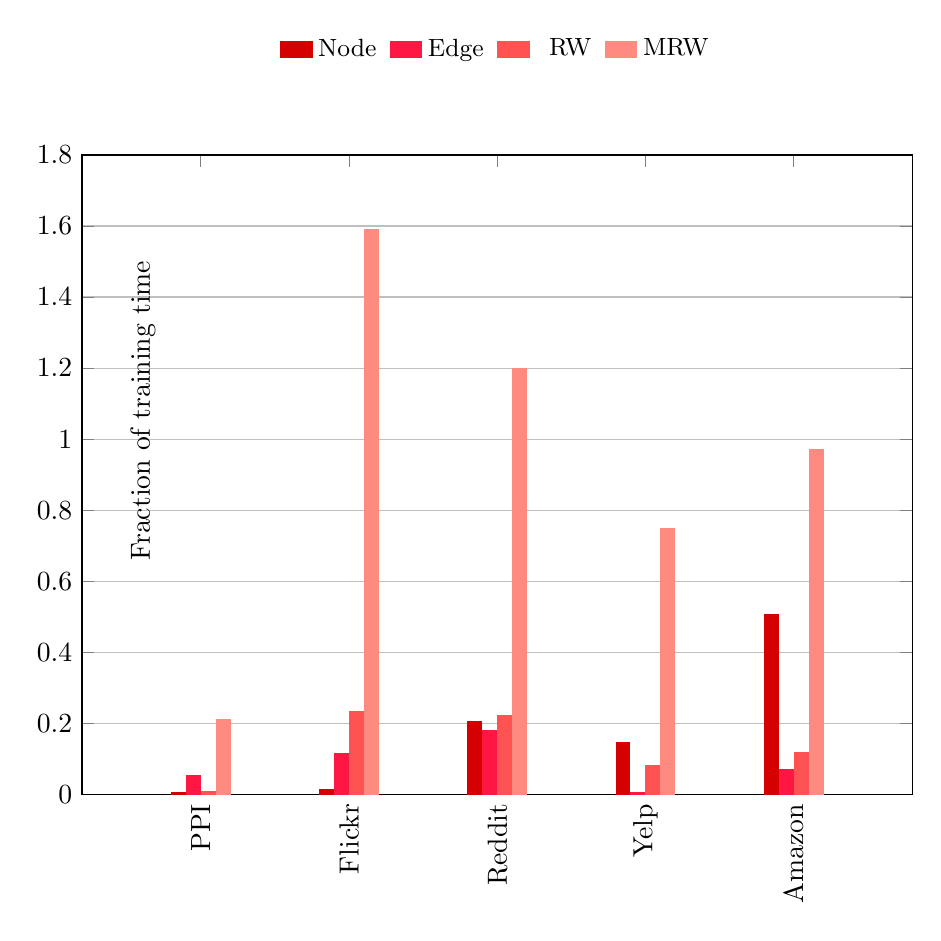
\begin{tikzpicture}
\begin{axis}[
    enlarge x limits=0.2,ymin=0,ymax=1.8,
    ybar=\pgflinewidth,
    tick align=inside,
    xtick=data,
    x tick label style={rotate=90},
    bar width=5pt,
    ymajorgrids = true,
    symbolic x coords={PPI, Flickr, Reddit, Yelp, Amazon},
    ylabel=Fraction of training time,
    width=\textwidth,
    height=0.8\textwidth,
    y label style={at={(axis description cs:0.1,.6)},anchor=south},
    yticklabel style={/pgf/number format/precision=2,/pgf/number format/fixed},
    legend style={font=\small},
    legend cell align=left,
    legend columns=5,
    legend style={at={(0.5,1.2)},anchor=north,/tikz/column 5/.style={column sep=5pt},draw=none,/tikz/every even column/.append style={column sep=0.1cm}}]
\addplot[style={skyblue,fill=skyblue,mark=none}]
            coordinates {(PPI,.006) (Flickr,.012) (Reddit,0.205) (Yelp,.145) (Amazon, 0.506)};
\addplot[style={yellowgreen,fill=yellowgreen,mark=none}]
            coordinates {(PPI,0.053) (Flickr,0.114) (Reddit,0.178) (Yelp,.006)(Amazon,0.07)};  
\addplot[style={darkyellow,fill=darkyellow,mark=none}]
            coordinates {(PPI, .007) (Flickr,.232) (Reddit,.222) (Yelp,.08)(Amazon,0.116)};  
% \addplot[style={orange,fill=orange,mark=none}]
%             coordinates {(PPI, .08436/2) (Flickr,.24003/2) (Reddit,.13430/2) (Yelp,.25785/2)};  
\addplot[style={orange,fill=orange,mark=none}]
            coordinates {(PPI, .21) (Flickr,1.59) (Reddit,1.20) (Yelp,.747)(Amazon,0.970)};  
            
\legend{Node,Edge,RW,MRW}
\pgfplotsset{
    legend image code/.code={
        \draw [#1] (0cm,-0.1cm) rectangle (0.4cm,0.1cm);
    },
}
\end{axis}
\fill [white] (0.1,-0.5) rectangle (0.2,-1.44);%-0.5,-1.34
\end{tikzpicture}
  %\vspace{-.3cm}
  \caption{Fraction of training time on sampling\label{fig: preproc cost}}
\end{minipage}
\end{figure}

\subsection{Training Efficiency on Deep Models}
\label{appendix: depth}
We evaluate the training efficiency for deeper GCNs. 
We only compare with S-GCN, since implementations for other layer sampling based methods have not yet supported arbitrary model depth. 
The batch size and hidden dimension are the same as Table \ref{tab: exp-sota}. 
On the two large graphs (Reddit and Yelp), we increase the number of layers and measure the average time per minibatch execution. In Figure \ref{fig: exp sota depth}, training cost of {\graphsaint} is approximately linear with GCN depth. Training cost of S-GCN grows dramatically when increasing the depth. This reflects the ``neighbor explosion'' phenomenon (even though the expansion factor of S-GCN is just 2). On Yelp, S-GCN gives ``out-of-memory'' error for models beyond 5 layers.


\subsection{Cost of Sampling and Pre-Processing}
\label{appendix: sampler cost}

\paragraph{Cost of graph samplers of {\graphsaint}} Graph sampling introduces little training overhead.
Let $t_s$ be the average time to sample one subgraph on a multi-core machine. Let $t_t$ be the average time to perform the forward and backward propagation on one minibatch on GPU. 
Figure \ref{fig: preproc cost} shows the ratio $t_s/t_t$ for various datasets. The parameters of the samplers are the same as Table \ref{tab: exp-sota}. For Node, Edge and RW samplers, we observe that time to sample one subgraph is in most cases less than 25\% of the training time. 
The MRW sampler is more expensive to execute. 
Regarding the complete pre-processing procedure, we repeatedly run the sampler for $N=50\cdot \size{\V}/\overline{\size{\V[s]}}$ times before training, to estimate the node and edge probability as discussed in Section \ref{sec: bias} (where $\overline{\size{\V[s]}}$ is the average subgraph size). These sampled subgraphs are reused as training minibatches. Thus, if training runs for more than $N$ iterations, the pre-processing is nearly zero-cost. 
Under the setting of Table \ref{tab: exp-sota}, pre-processing on PPI and Yelp and Amazon does not incur any overhead in training time. Pre-processing on Flickr and Reddit (with RW sampler) takes less than 40\% and 15\% of their corresponding total training time. 

\paragraph{Cost of layers sampler of AS-GCN}
AS-GCN uses an additional neural network to estimate the conditional sampling probability for the previous layer. For a node $v$ already sampled in layer $\ell$, features of layer-$\paren{\ell-1}$ corresponding to all $v$'s neighbors need to be fed to the sampling neural network to obtain the node probability. For sake of analysis, assume the sampling network is a single layer MLP, whose weight $\bm{W}_\text{MLP}$ has the same shape as the GCN weights $\bm{W}^{\paren{\ell}}$. 
Then we can show, for a $L$-layer GCN on a degree-$d$ graph, per epoch training complexity of AS-GCN is approximately $\gamma=\paren{d\cdot L}/\sum_{\ell=0}^{L-1}d^\ell$ times that of vanilla GCN. For $L=2$, we have $\gamma\approx 2$. This explains the observation that AS-GCN is slower than vanilla GCN in Figure \ref{fig: 2 layer convergence}. Additional, Table \ref{tab: asgcn breakdown} shows the training time breakdown for AS-GCN. Clearly, its sampler is much more expensive than the graph sampler of {\graphsaint}. 

\begin{table*}[!ht]
\caption{Per epoch training time breakdown for AS-GCN}
    \centering
    %\resizebox{1.0\textwidth}{!}{
    \begin{tabular}{rcc}
        \toprule
        \multirow{2}{*}{Dataset} & \multirow{2}{*}{Sampling time (sec)} & {Forward / Backward}\\
        & & propagation time (sec)\\
        \midrule
        \midrule
        PPI & 1.1 & 0.2 \\
        Flickr & 5.3 & 1.1\\
        Reddit & 20.7 & 3.5 \\
        \bottomrule
    \end{tabular}%}
    \label{tab: asgcn breakdown}
\end{table*}


\paragraph{Cost of clustering of ClusterGCN}
ClusterGCN uses the highly optimized METIS software\footnote{\url{http://glaros.dtc.umn.edu/gkhome/metis/metis/download}} to perform clustering. Table \ref{tab: cluster cost} summarizes the time to obtain the clusters for the five graphs. On the large and dense Amazon graph, the cost of clustering increase dramatically. The pre-processing time of ClusterGCN on Amazon is more than $4\times$ of the total training time. On the other hand, the sampling cost of {\graphsaint} does not increase significantly for large graphs (see Figure \ref{fig: preproc cost}). 

\begin{table*}[!ht]
\caption{Clustering time of ClusterGCN}
    \centering
    %\resizebox{1.0\textwidth}{!}{
    \begin{tabular}{rccccc}
        \toprule
        & PPI & Flickr & Reddit & Yelp & Amazon\\
        \midrule
        \midrule
        Time (sec) & 2.2 & 11.6 & 40.0 & 106.7 & 2254.2\\
        \bottomrule
    \end{tabular}%}
    \label{tab: cluster cost}
\end{table*}


Taking into account the pre-processing time, sampling time and training time altogether, we summarize the total convergence time of {\graphsaint} and ClusterGCN in Table \ref{tab: appendix-tot-time-saint-cluster} (corresponding to Table \ref{tab: exp-sota} configuration). 
On graphs that are large and dense (e.g., Amazon), {\graphsaint} achieves significantly faster convergence. 
Note that both the sampling of {\graphsaint} and clustering of ClusterGCN can be performed offline. 

\begin{table*}[!ht]
\caption{Comparison of total convergence time (pre-processing + sampling + training, unit: second)}
    \centering
    %\resizebox{1.0\textwidth}{!}{
    \begin{tabular}{rccccc}
        \toprule
        & PPI & Flickr & Reddit & Yelp & Amazon\\
        \midrule
        \midrule
        {\graphsaint}-{\small Edge} & 91.0 & 7.0 & 16.6 & 273.9 & 401.0\\
        {\graphsaint}-{\small RW} & 103.6 & 7.5 & 17.2 & 310.1 & 425.6 \\
        ClusterGCN & 163.2 & 12.9 & 55.3 & 256.0 & 2804.8\\
        \bottomrule
    \end{tabular}%}
    \label{tab: appendix-tot-time-saint-cluster}
\end{table*}



\subsection{Effect of Batch Size}
\label{appendix: batch size}
\begin{table*}[!ht]
\caption{Test set F1-micro for the baselines under various batch sizes}
    \centering
    %\resizebox{1.0\textwidth}{!}{
    \begin{tabular}{rcccccc}
        \toprule
        {Method} & {Batch size} & {PPI} & {Flickr} & {Reddit} & {Yelp} & Amazon\\
        \midrule
        \midrule
        \multirow{4}{*}{GraphSAGE} & 256 & 0.600 & 0.474 & 0.934 & 0.563 & 0.428\\
         & 512\footnotemark[1] & 0.637 & 0.501 & 0.953 & 0.634 & 0.758\\
         & 1024 & 0.610 & 0.482 & 0.935 & 0.632 & 0.705\\
         & 2048 & 0.625 & 0.374 & 0.936 & 0.563 & 0.447\\
         \midrule
        \multirow{3}{*}{FastGCN} & 400\footnotemark[1] & 0.513 & 0.504 & 0.924 & 0.265 & 0.174\\
        & 2000 & 0.561 & 0.506  & 0.934 & 0.255 & 0.196\\
        & 4000 & 0.564 & 0.507  & 0.934 & 0.260 & 0.195\\
        \midrule
        % S-GCN-{\small{500}} \cite{s-gcn} & 0.519 & 12 & 0.462 & 6 & 0.224 & 80 & 0.000 & 80\\
        % \multirow{4}{*}{S-GCN} & 1000 & 0.963 & 40 & 0.464 & 8 & 0.964 & 119 & 0.640 & 117\\
        % & 2000 & 0.646 & 12 & 0.485 & 12 & 0.949 & 86 & 0.614 & 69\\
        % & 4000 & 0.804 & 30 & 0.482 & 4 & 0.949 & 86 & 0.594 & 60\\
        % & 8000 & 0.694 & 16 & 0.483 & 13 & 0.950 & 96 & 0.613 & 76\\
        \multirow{5}{*}{S-GCN} & 500 & 0.519 & 0.462 & ---\footnotemark[5] & ---\footnotemark[5] & ---\footnotemark[3]\\
         & 1000\footnotemark[1] & 0.963 & 0.482 & 0.964 & 0.640 & ---\footnotemark[3] \\
         & 2000 & 0.646 & 0.482 & 0.949 & 0.614 & ---\footnotemark[3] \\
         & 4000 & 0.804 & 0.482 & 0.949 & 0.594 & ---\footnotemark[3] \\
         & 8000 & 0.694 & 0.481 & 0.950 & 0.613 & ---\footnotemark[3] \\
        \midrule
        \multirow{4}{*}{AS-GCN} & 256 & 0.682 & 0.504 & 0.950 & ---\footnotemark[3] & ---\footnotemark[3] \\
         & 512\footnotemark[1] & 0.687 & 0.504 & 0.958 & ---\footnotemark[3] & ---\footnotemark[3]\\
         & 1024 & 0.687 & 0.502 & 0.951 & ---\footnotemark[3] & ---\footnotemark[3]\\
         & 2048 & 0.670 & 0.502 & 0.952 & ---\footnotemark[3] & ---\footnotemark[3]\\
        \midrule
        \multirow{8}{*}{ClusterGCN} & 500 & 0.875 & 0.481 & 0.942 & 0.604 & 0.752\\
         & 1000 & 0.831 & 0.478 & 0.947 & 0.602 & 0.756 \\
         & 1500 & 0.865 & 0.480 & 0.954 & 0.602 & 0.752\\
         & 2000 & 0.828 & 0.469 & 0.954 & 0.609 & 0.759\\
         & 2500 & 0.849 & 0.476 & 0.954 & 0.598 & 0.745\\
         & 3000 & 0.840 & 0.473 & 0.954 & 0.607 & 0.754\\
         & 3500 & 0.846 & 0.473 & 0.952 & 0.602 & 0.754\\
         & 4000 & 0.853 & 0.472 & 0.949 & 0.605 & 0.756\\
        \bottomrule
    \end{tabular}%}
    \label{tab: exp-fastgcn-batch}
\end{table*}

\footnotetext[1]{Default batch size}
\footnotetext[5]{The training does not converge.}
\footnotetext[3]{The codes throw runtime error on the large datasets (Yelp or Amazon).}


% \begin{figure}
% \centering
% \resizebox{\textwidth}{!}{%% Creator: Matplotlib, PGF backend
%%
%% To include the figure in your LaTeX document, write
%%   \input{<filename>.pgf}
%%
%% Make sure the required packages are loaded in your preamble
%%   \usepackage{pgf}
%%
%% Figures using additional raster images can only be included by \input if
%% they are in the same directory as the main LaTeX file. For loading figures
%% from other directories you can use the `import` package
%%   \usepackage{import}
%% and then include the figures with
%%   \import{<path to file>}{<filename>.pgf}
%%
%% Matplotlib used the following preamble
%%   \usepackage[utf8x]{inputenc}
%%   \usepackage[T1]{fontenc}
%%   \usepackage{cmbright}
%%   \usepackage{amsmath}
%%
\begingroup%
\makeatletter%
\begin{pgfpicture}%
\pgfpathrectangle{\pgfpointorigin}{\pgfqpoint{10.000000in}{8.000000in}}%
\pgfusepath{use as bounding box, clip}%
\begin{pgfscope}%
\pgfsetbuttcap%
\pgfsetmiterjoin%
\definecolor{currentfill}{rgb}{1.000000,1.000000,1.000000}%
\pgfsetfillcolor{currentfill}%
\pgfsetlinewidth{0.000000pt}%
\definecolor{currentstroke}{rgb}{1.000000,1.000000,1.000000}%
\pgfsetstrokecolor{currentstroke}%
\pgfsetdash{}{0pt}%
\pgfpathmoveto{\pgfqpoint{0.000000in}{0.000000in}}%
\pgfpathlineto{\pgfqpoint{10.000000in}{0.000000in}}%
\pgfpathlineto{\pgfqpoint{10.000000in}{8.000000in}}%
\pgfpathlineto{\pgfqpoint{0.000000in}{8.000000in}}%
\pgfpathclose%
\pgfusepath{fill}%
\end{pgfscope}%
\begin{pgfscope}%
\pgfsetbuttcap%
\pgfsetmiterjoin%
\definecolor{currentfill}{rgb}{1.000000,1.000000,1.000000}%
\pgfsetfillcolor{currentfill}%
\pgfsetlinewidth{0.000000pt}%
\definecolor{currentstroke}{rgb}{0.000000,0.000000,0.000000}%
\pgfsetstrokecolor{currentstroke}%
\pgfsetstrokeopacity{0.000000}%
\pgfsetdash{}{0pt}%
\pgfpathmoveto{\pgfqpoint{1.250000in}{4.240000in}}%
\pgfpathlineto{\pgfqpoint{4.772727in}{4.240000in}}%
\pgfpathlineto{\pgfqpoint{4.772727in}{7.040000in}}%
\pgfpathlineto{\pgfqpoint{1.250000in}{7.040000in}}%
\pgfpathclose%
\pgfusepath{fill}%
\end{pgfscope}%
\begin{pgfscope}%
\pgfpathrectangle{\pgfqpoint{1.250000in}{4.240000in}}{\pgfqpoint{3.522727in}{2.800000in}}%
\pgfusepath{clip}%
\pgfsetbuttcap%
\pgfsetmiterjoin%
\pgfsetlinewidth{1.003750pt}%
\definecolor{currentstroke}{rgb}{0.500000,0.500000,0.500000}%
\pgfsetstrokecolor{currentstroke}%
\pgfsetdash{}{0pt}%
\pgfpathmoveto{\pgfqpoint{4.367614in}{6.872000in}}%
\pgfpathlineto{\pgfqpoint{4.402841in}{6.872000in}}%
\pgfpathlineto{\pgfqpoint{4.402841in}{6.967200in}}%
\pgfpathlineto{\pgfqpoint{4.367614in}{6.967200in}}%
\pgfpathlineto{\pgfqpoint{4.367614in}{6.872000in}}%
\pgfpathclose%
\pgfusepath{stroke}%
\end{pgfscope}%
\begin{pgfscope}%
\pgfpathrectangle{\pgfqpoint{1.250000in}{4.240000in}}{\pgfqpoint{3.522727in}{2.800000in}}%
\pgfusepath{clip}%
\pgfsetrectcap%
\pgfsetroundjoin%
\pgfsetlinewidth{0.803000pt}%
\definecolor{currentstroke}{rgb}{0.690196,0.690196,0.690196}%
\pgfsetstrokecolor{currentstroke}%
\pgfsetdash{}{0pt}%
\pgfpathmoveto{\pgfqpoint{1.250000in}{4.240000in}}%
\pgfpathlineto{\pgfqpoint{1.250000in}{7.040000in}}%
\pgfusepath{stroke}%
\end{pgfscope}%
\begin{pgfscope}%
\definecolor{textcolor}{rgb}{0.000000,0.000000,0.000000}%
\pgfsetstrokecolor{textcolor}%
\pgfsetfillcolor{textcolor}%
\pgftext[x=1.250000in,y=4.191389in,,top]{\color{textcolor}\rmfamily\fontsize{14.000000}{16.800000}\selectfont 0}%
\end{pgfscope}%
\begin{pgfscope}%
\pgfpathrectangle{\pgfqpoint{1.250000in}{4.240000in}}{\pgfqpoint{3.522727in}{2.800000in}}%
\pgfusepath{clip}%
\pgfsetrectcap%
\pgfsetroundjoin%
\pgfsetlinewidth{0.803000pt}%
\definecolor{currentstroke}{rgb}{0.690196,0.690196,0.690196}%
\pgfsetstrokecolor{currentstroke}%
\pgfsetdash{}{0pt}%
\pgfpathmoveto{\pgfqpoint{2.130682in}{4.240000in}}%
\pgfpathlineto{\pgfqpoint{2.130682in}{7.040000in}}%
\pgfusepath{stroke}%
\end{pgfscope}%
\begin{pgfscope}%
\definecolor{textcolor}{rgb}{0.000000,0.000000,0.000000}%
\pgfsetstrokecolor{textcolor}%
\pgfsetfillcolor{textcolor}%
\pgftext[x=2.130682in,y=4.191389in,,top]{\color{textcolor}\rmfamily\fontsize{14.000000}{16.800000}\selectfont 50}%
\end{pgfscope}%
\begin{pgfscope}%
\pgfpathrectangle{\pgfqpoint{1.250000in}{4.240000in}}{\pgfqpoint{3.522727in}{2.800000in}}%
\pgfusepath{clip}%
\pgfsetrectcap%
\pgfsetroundjoin%
\pgfsetlinewidth{0.803000pt}%
\definecolor{currentstroke}{rgb}{0.690196,0.690196,0.690196}%
\pgfsetstrokecolor{currentstroke}%
\pgfsetdash{}{0pt}%
\pgfpathmoveto{\pgfqpoint{3.011364in}{4.240000in}}%
\pgfpathlineto{\pgfqpoint{3.011364in}{7.040000in}}%
\pgfusepath{stroke}%
\end{pgfscope}%
\begin{pgfscope}%
\definecolor{textcolor}{rgb}{0.000000,0.000000,0.000000}%
\pgfsetstrokecolor{textcolor}%
\pgfsetfillcolor{textcolor}%
\pgftext[x=3.011364in,y=4.191389in,,top]{\color{textcolor}\rmfamily\fontsize{14.000000}{16.800000}\selectfont 100}%
\end{pgfscope}%
\begin{pgfscope}%
\pgfpathrectangle{\pgfqpoint{1.250000in}{4.240000in}}{\pgfqpoint{3.522727in}{2.800000in}}%
\pgfusepath{clip}%
\pgfsetrectcap%
\pgfsetroundjoin%
\pgfsetlinewidth{0.803000pt}%
\definecolor{currentstroke}{rgb}{0.690196,0.690196,0.690196}%
\pgfsetstrokecolor{currentstroke}%
\pgfsetdash{}{0pt}%
\pgfpathmoveto{\pgfqpoint{3.892045in}{4.240000in}}%
\pgfpathlineto{\pgfqpoint{3.892045in}{7.040000in}}%
\pgfusepath{stroke}%
\end{pgfscope}%
\begin{pgfscope}%
\definecolor{textcolor}{rgb}{0.000000,0.000000,0.000000}%
\pgfsetstrokecolor{textcolor}%
\pgfsetfillcolor{textcolor}%
\pgftext[x=3.892045in,y=4.191389in,,top]{\color{textcolor}\rmfamily\fontsize{14.000000}{16.800000}\selectfont 150}%
\end{pgfscope}%
\begin{pgfscope}%
\pgfpathrectangle{\pgfqpoint{1.250000in}{4.240000in}}{\pgfqpoint{3.522727in}{2.800000in}}%
\pgfusepath{clip}%
\pgfsetrectcap%
\pgfsetroundjoin%
\pgfsetlinewidth{0.803000pt}%
\definecolor{currentstroke}{rgb}{0.690196,0.690196,0.690196}%
\pgfsetstrokecolor{currentstroke}%
\pgfsetdash{}{0pt}%
\pgfpathmoveto{\pgfqpoint{4.772727in}{4.240000in}}%
\pgfpathlineto{\pgfqpoint{4.772727in}{7.040000in}}%
\pgfusepath{stroke}%
\end{pgfscope}%
\begin{pgfscope}%
\definecolor{textcolor}{rgb}{0.000000,0.000000,0.000000}%
\pgfsetstrokecolor{textcolor}%
\pgfsetfillcolor{textcolor}%
\pgftext[x=4.772727in,y=4.191389in,,top]{\color{textcolor}\rmfamily\fontsize{14.000000}{16.800000}\selectfont 200}%
\end{pgfscope}%
\begin{pgfscope}%
\pgfpathrectangle{\pgfqpoint{1.250000in}{4.240000in}}{\pgfqpoint{3.522727in}{2.800000in}}%
\pgfusepath{clip}%
\pgfsetrectcap%
\pgfsetroundjoin%
\pgfsetlinewidth{0.803000pt}%
\definecolor{currentstroke}{rgb}{0.690196,0.690196,0.690196}%
\pgfsetstrokecolor{currentstroke}%
\pgfsetdash{}{0pt}%
\pgfpathmoveto{\pgfqpoint{1.250000in}{4.240000in}}%
\pgfpathlineto{\pgfqpoint{4.772727in}{4.240000in}}%
\pgfusepath{stroke}%
\end{pgfscope}%
\begin{pgfscope}%
\definecolor{textcolor}{rgb}{0.000000,0.000000,0.000000}%
\pgfsetstrokecolor{textcolor}%
\pgfsetfillcolor{textcolor}%
\pgftext[x=0.958174in,y=4.171134in,left,base]{\color{textcolor}\rmfamily\fontsize{14.000000}{16.800000}\selectfont 0.5}%
\end{pgfscope}%
\begin{pgfscope}%
\pgfpathrectangle{\pgfqpoint{1.250000in}{4.240000in}}{\pgfqpoint{3.522727in}{2.800000in}}%
\pgfusepath{clip}%
\pgfsetrectcap%
\pgfsetroundjoin%
\pgfsetlinewidth{0.803000pt}%
\definecolor{currentstroke}{rgb}{0.690196,0.690196,0.690196}%
\pgfsetstrokecolor{currentstroke}%
\pgfsetdash{}{0pt}%
\pgfpathmoveto{\pgfqpoint{1.250000in}{4.800000in}}%
\pgfpathlineto{\pgfqpoint{4.772727in}{4.800000in}}%
\pgfusepath{stroke}%
\end{pgfscope}%
\begin{pgfscope}%
\definecolor{textcolor}{rgb}{0.000000,0.000000,0.000000}%
\pgfsetstrokecolor{textcolor}%
\pgfsetfillcolor{textcolor}%
\pgftext[x=0.958174in,y=4.731134in,left,base]{\color{textcolor}\rmfamily\fontsize{14.000000}{16.800000}\selectfont 0.6}%
\end{pgfscope}%
\begin{pgfscope}%
\pgfpathrectangle{\pgfqpoint{1.250000in}{4.240000in}}{\pgfqpoint{3.522727in}{2.800000in}}%
\pgfusepath{clip}%
\pgfsetrectcap%
\pgfsetroundjoin%
\pgfsetlinewidth{0.803000pt}%
\definecolor{currentstroke}{rgb}{0.690196,0.690196,0.690196}%
\pgfsetstrokecolor{currentstroke}%
\pgfsetdash{}{0pt}%
\pgfpathmoveto{\pgfqpoint{1.250000in}{5.360000in}}%
\pgfpathlineto{\pgfqpoint{4.772727in}{5.360000in}}%
\pgfusepath{stroke}%
\end{pgfscope}%
\begin{pgfscope}%
\definecolor{textcolor}{rgb}{0.000000,0.000000,0.000000}%
\pgfsetstrokecolor{textcolor}%
\pgfsetfillcolor{textcolor}%
\pgftext[x=0.958174in,y=5.291134in,left,base]{\color{textcolor}\rmfamily\fontsize{14.000000}{16.800000}\selectfont 0.7}%
\end{pgfscope}%
\begin{pgfscope}%
\pgfpathrectangle{\pgfqpoint{1.250000in}{4.240000in}}{\pgfqpoint{3.522727in}{2.800000in}}%
\pgfusepath{clip}%
\pgfsetrectcap%
\pgfsetroundjoin%
\pgfsetlinewidth{0.803000pt}%
\definecolor{currentstroke}{rgb}{0.690196,0.690196,0.690196}%
\pgfsetstrokecolor{currentstroke}%
\pgfsetdash{}{0pt}%
\pgfpathmoveto{\pgfqpoint{1.250000in}{5.920000in}}%
\pgfpathlineto{\pgfqpoint{4.772727in}{5.920000in}}%
\pgfusepath{stroke}%
\end{pgfscope}%
\begin{pgfscope}%
\definecolor{textcolor}{rgb}{0.000000,0.000000,0.000000}%
\pgfsetstrokecolor{textcolor}%
\pgfsetfillcolor{textcolor}%
\pgftext[x=0.958174in,y=5.851134in,left,base]{\color{textcolor}\rmfamily\fontsize{14.000000}{16.800000}\selectfont 0.8}%
\end{pgfscope}%
\begin{pgfscope}%
\pgfpathrectangle{\pgfqpoint{1.250000in}{4.240000in}}{\pgfqpoint{3.522727in}{2.800000in}}%
\pgfusepath{clip}%
\pgfsetrectcap%
\pgfsetroundjoin%
\pgfsetlinewidth{0.803000pt}%
\definecolor{currentstroke}{rgb}{0.690196,0.690196,0.690196}%
\pgfsetstrokecolor{currentstroke}%
\pgfsetdash{}{0pt}%
\pgfpathmoveto{\pgfqpoint{1.250000in}{6.480000in}}%
\pgfpathlineto{\pgfqpoint{4.772727in}{6.480000in}}%
\pgfusepath{stroke}%
\end{pgfscope}%
\begin{pgfscope}%
\definecolor{textcolor}{rgb}{0.000000,0.000000,0.000000}%
\pgfsetstrokecolor{textcolor}%
\pgfsetfillcolor{textcolor}%
\pgftext[x=0.958174in,y=6.411134in,left,base]{\color{textcolor}\rmfamily\fontsize{14.000000}{16.800000}\selectfont 0.9}%
\end{pgfscope}%
\begin{pgfscope}%
\pgfpathrectangle{\pgfqpoint{1.250000in}{4.240000in}}{\pgfqpoint{3.522727in}{2.800000in}}%
\pgfusepath{clip}%
\pgfsetrectcap%
\pgfsetroundjoin%
\pgfsetlinewidth{0.803000pt}%
\definecolor{currentstroke}{rgb}{0.690196,0.690196,0.690196}%
\pgfsetstrokecolor{currentstroke}%
\pgfsetdash{}{0pt}%
\pgfpathmoveto{\pgfqpoint{1.250000in}{7.040000in}}%
\pgfpathlineto{\pgfqpoint{4.772727in}{7.040000in}}%
\pgfusepath{stroke}%
\end{pgfscope}%
\begin{pgfscope}%
\definecolor{textcolor}{rgb}{0.000000,0.000000,0.000000}%
\pgfsetstrokecolor{textcolor}%
\pgfsetfillcolor{textcolor}%
\pgftext[x=0.958174in,y=6.971134in,left,base]{\color{textcolor}\rmfamily\fontsize{14.000000}{16.800000}\selectfont 1.0}%
\end{pgfscope}%
\begin{pgfscope}%
\definecolor{textcolor}{rgb}{0.000000,0.000000,0.000000}%
\pgfsetstrokecolor{textcolor}%
\pgfsetfillcolor{textcolor}%
\pgftext[x=0.902619in,y=5.640000in,,bottom,rotate=90.000000]{\color{textcolor}\rmfamily\fontsize{14.000000}{16.800000}\selectfont Validation \(\displaystyle \text{F1}_{\text{mic}}\)}%
\end{pgfscope}%
\begin{pgfscope}%
\pgfpathrectangle{\pgfqpoint{1.250000in}{4.240000in}}{\pgfqpoint{3.522727in}{2.800000in}}%
\pgfusepath{clip}%
\pgfsetrectcap%
\pgfsetroundjoin%
\pgfsetlinewidth{1.505625pt}%
\definecolor{currentstroke}{rgb}{0.000000,0.000000,1.000000}%
\pgfsetstrokecolor{currentstroke}%
\pgfsetdash{}{0pt}%
\pgfpathmoveto{\pgfqpoint{1.500214in}{4.230000in}}%
\pgfpathlineto{\pgfqpoint{1.502604in}{4.240056in}}%
\pgfpathlineto{\pgfqpoint{1.522740in}{4.232496in}}%
\pgfpathlineto{\pgfqpoint{1.542980in}{4.302216in}}%
\pgfpathlineto{\pgfqpoint{1.549103in}{4.230000in}}%
\pgfpathmoveto{\pgfqpoint{1.582900in}{4.230000in}}%
\pgfpathlineto{\pgfqpoint{1.583526in}{4.235184in}}%
\pgfpathlineto{\pgfqpoint{1.603771in}{4.286760in}}%
\pgfpathlineto{\pgfqpoint{1.624130in}{4.409400in}}%
\pgfpathlineto{\pgfqpoint{1.644624in}{4.505496in}}%
\pgfpathlineto{\pgfqpoint{1.665108in}{4.230000in}}%
\pgfpathmoveto{\pgfqpoint{1.665688in}{4.230000in}}%
\pgfpathlineto{\pgfqpoint{1.685774in}{4.424800in}}%
\pgfpathlineto{\pgfqpoint{1.706008in}{4.301264in}}%
\pgfpathlineto{\pgfqpoint{1.725642in}{4.495360in}}%
\pgfpathlineto{\pgfqpoint{1.746153in}{4.272760in}}%
\pgfpathlineto{\pgfqpoint{1.766548in}{4.538592in}}%
\pgfpathlineto{\pgfqpoint{1.786292in}{4.608088in}}%
\pgfpathlineto{\pgfqpoint{1.805906in}{4.360736in}}%
\pgfpathlineto{\pgfqpoint{1.826032in}{4.605512in}}%
\pgfpathlineto{\pgfqpoint{1.845974in}{4.474360in}}%
\pgfpathlineto{\pgfqpoint{1.866887in}{4.526048in}}%
\pgfpathlineto{\pgfqpoint{1.886868in}{4.649584in}}%
\pgfpathlineto{\pgfqpoint{1.907103in}{4.443952in}}%
\pgfpathlineto{\pgfqpoint{1.927750in}{4.566928in}}%
\pgfpathlineto{\pgfqpoint{1.947686in}{4.544360in}}%
\pgfpathlineto{\pgfqpoint{1.967811in}{4.680272in}}%
\pgfpathlineto{\pgfqpoint{1.987843in}{4.572976in}}%
\pgfpathlineto{\pgfqpoint{2.007590in}{4.592856in}}%
\pgfpathlineto{\pgfqpoint{2.026987in}{4.669576in}}%
\pgfpathlineto{\pgfqpoint{2.047258in}{4.783928in}}%
\pgfpathlineto{\pgfqpoint{2.067692in}{4.650256in}}%
\pgfpathlineto{\pgfqpoint{2.088358in}{4.702224in}}%
\pgfpathlineto{\pgfqpoint{2.108971in}{4.748984in}}%
\pgfpathlineto{\pgfqpoint{2.129604in}{4.780176in}}%
\pgfpathlineto{\pgfqpoint{2.149370in}{4.746968in}}%
\pgfpathlineto{\pgfqpoint{2.169359in}{4.856672in}}%
\pgfpathlineto{\pgfqpoint{2.189483in}{4.775696in}}%
\pgfpathlineto{\pgfqpoint{2.209433in}{4.734032in}}%
\pgfpathlineto{\pgfqpoint{2.229773in}{4.850904in}}%
\pgfpathlineto{\pgfqpoint{2.249593in}{4.776368in}}%
\pgfpathlineto{\pgfqpoint{2.269409in}{4.888256in}}%
\pgfpathlineto{\pgfqpoint{2.289544in}{4.827888in}}%
\pgfpathlineto{\pgfqpoint{2.309620in}{4.943080in}}%
\pgfpathlineto{\pgfqpoint{2.329185in}{4.892400in}}%
\pgfpathlineto{\pgfqpoint{2.349146in}{4.924656in}}%
\pgfpathlineto{\pgfqpoint{2.368896in}{4.929920in}}%
\pgfpathlineto{\pgfqpoint{2.388346in}{4.900296in}}%
\pgfpathlineto{\pgfqpoint{2.407600in}{4.982224in}}%
\pgfpathlineto{\pgfqpoint{2.427138in}{5.006584in}}%
\pgfpathlineto{\pgfqpoint{2.446524in}{4.982112in}}%
\pgfpathlineto{\pgfqpoint{2.466574in}{4.987488in}}%
\pgfpathlineto{\pgfqpoint{2.485937in}{5.123064in}}%
\pgfpathlineto{\pgfqpoint{2.505146in}{4.948176in}}%
\pgfpathlineto{\pgfqpoint{2.524163in}{4.908024in}}%
\pgfpathlineto{\pgfqpoint{2.543377in}{4.909480in}}%
\pgfpathlineto{\pgfqpoint{2.562956in}{5.015432in}}%
\pgfpathlineto{\pgfqpoint{2.582206in}{4.956240in}}%
\pgfpathlineto{\pgfqpoint{2.601813in}{5.032792in}}%
\pgfpathlineto{\pgfqpoint{2.621196in}{5.103296in}}%
\pgfpathlineto{\pgfqpoint{2.641114in}{5.027528in}}%
\pgfpathlineto{\pgfqpoint{2.661167in}{5.118416in}}%
\pgfpathlineto{\pgfqpoint{2.680772in}{5.084200in}}%
\pgfpathlineto{\pgfqpoint{2.700352in}{5.136280in}}%
\pgfpathlineto{\pgfqpoint{2.740163in}{5.084256in}}%
\pgfpathlineto{\pgfqpoint{2.759604in}{5.139416in}}%
\pgfpathlineto{\pgfqpoint{2.778991in}{5.158400in}}%
\pgfpathlineto{\pgfqpoint{2.798325in}{5.078040in}}%
\pgfpathlineto{\pgfqpoint{2.817756in}{5.093664in}}%
\pgfpathlineto{\pgfqpoint{2.836767in}{5.118136in}}%
\pgfpathlineto{\pgfqpoint{2.856000in}{5.187632in}}%
\pgfpathlineto{\pgfqpoint{2.875964in}{5.221064in}}%
\pgfpathlineto{\pgfqpoint{2.895363in}{5.202416in}}%
\pgfpathlineto{\pgfqpoint{2.914945in}{5.179848in}}%
\pgfpathlineto{\pgfqpoint{2.934114in}{5.204992in}}%
\pgfpathlineto{\pgfqpoint{2.953730in}{5.285800in}}%
\pgfpathlineto{\pgfqpoint{2.973152in}{5.205440in}}%
\pgfpathlineto{\pgfqpoint{2.992532in}{5.194352in}}%
\pgfpathlineto{\pgfqpoint{3.012225in}{5.236128in}}%
\pgfpathlineto{\pgfqpoint{3.031928in}{5.228176in}}%
\pgfpathlineto{\pgfqpoint{3.051329in}{5.224928in}}%
\pgfpathlineto{\pgfqpoint{3.070428in}{5.142944in}}%
\pgfpathlineto{\pgfqpoint{3.089776in}{5.310608in}}%
\pgfpathlineto{\pgfqpoint{3.108889in}{5.170888in}}%
\pgfpathlineto{\pgfqpoint{3.128234in}{5.255840in}}%
\pgfpathlineto{\pgfqpoint{3.147355in}{5.173296in}}%
\pgfpathlineto{\pgfqpoint{3.167026in}{5.284848in}}%
\pgfpathlineto{\pgfqpoint{3.187162in}{5.259200in}}%
\pgfpathlineto{\pgfqpoint{3.207016in}{5.289664in}}%
\pgfpathlineto{\pgfqpoint{3.226640in}{5.254776in}}%
\pgfpathlineto{\pgfqpoint{3.245962in}{5.333456in}}%
\pgfpathlineto{\pgfqpoint{3.265695in}{5.219216in}}%
\pgfpathlineto{\pgfqpoint{3.285256in}{5.328752in}}%
\pgfpathlineto{\pgfqpoint{3.305023in}{5.282328in}}%
\pgfpathlineto{\pgfqpoint{3.324928in}{5.265864in}}%
\pgfpathlineto{\pgfqpoint{3.344747in}{5.302488in}}%
\pgfpathlineto{\pgfqpoint{3.364615in}{5.251248in}}%
\pgfpathlineto{\pgfqpoint{3.384129in}{5.246432in}}%
\pgfpathlineto{\pgfqpoint{3.403429in}{5.294032in}}%
\pgfpathlineto{\pgfqpoint{3.422981in}{5.328024in}}%
\pgfpathlineto{\pgfqpoint{3.442310in}{5.275384in}}%
\pgfpathlineto{\pgfqpoint{3.461921in}{5.251696in}}%
\pgfpathlineto{\pgfqpoint{3.481316in}{5.269728in}}%
\pgfpathlineto{\pgfqpoint{3.501008in}{5.353672in}}%
\pgfpathlineto{\pgfqpoint{3.520587in}{5.334352in}}%
\pgfpathlineto{\pgfqpoint{3.539711in}{5.340960in}}%
\pgfpathlineto{\pgfqpoint{3.559361in}{5.299800in}}%
\pgfpathlineto{\pgfqpoint{3.578508in}{5.295040in}}%
\pgfpathlineto{\pgfqpoint{3.617747in}{5.375064in}}%
\pgfpathlineto{\pgfqpoint{3.637212in}{5.374112in}}%
\pgfpathlineto{\pgfqpoint{3.656734in}{5.334352in}}%
\pgfpathlineto{\pgfqpoint{3.675847in}{5.324720in}}%
\pgfpathlineto{\pgfqpoint{3.695160in}{5.371368in}}%
\pgfpathlineto{\pgfqpoint{3.714401in}{5.400208in}}%
\pgfpathlineto{\pgfqpoint{3.733761in}{5.397240in}}%
\pgfpathlineto{\pgfqpoint{3.752914in}{5.413984in}}%
\pgfpathlineto{\pgfqpoint{3.772378in}{5.371984in}}%
\pgfpathlineto{\pgfqpoint{3.791346in}{5.421880in}}%
\pgfpathlineto{\pgfqpoint{3.810800in}{5.429328in}}%
\pgfpathlineto{\pgfqpoint{3.829935in}{5.312344in}}%
\pgfpathlineto{\pgfqpoint{3.848998in}{5.368736in}}%
\pgfpathlineto{\pgfqpoint{3.868699in}{5.401216in}}%
\pgfpathlineto{\pgfqpoint{3.888198in}{5.447136in}}%
\pgfpathlineto{\pgfqpoint{3.907743in}{5.375008in}}%
\pgfpathlineto{\pgfqpoint{3.927120in}{5.366944in}}%
\pgfpathlineto{\pgfqpoint{3.946230in}{5.327968in}}%
\pgfpathlineto{\pgfqpoint{3.965276in}{5.341464in}}%
\pgfpathlineto{\pgfqpoint{3.984629in}{5.424344in}}%
\pgfpathlineto{\pgfqpoint{4.003966in}{5.419192in}}%
\pgfpathlineto{\pgfqpoint{4.023348in}{5.455480in}}%
\pgfpathlineto{\pgfqpoint{4.042279in}{5.435936in}}%
\pgfpathlineto{\pgfqpoint{4.061207in}{5.372376in}}%
\pgfpathlineto{\pgfqpoint{4.080340in}{5.430168in}}%
\pgfpathlineto{\pgfqpoint{4.099446in}{5.441088in}}%
\pgfpathlineto{\pgfqpoint{4.118606in}{5.383408in}}%
\pgfpathlineto{\pgfqpoint{4.137710in}{5.490648in}}%
\pgfpathlineto{\pgfqpoint{4.157426in}{5.444448in}}%
\pgfpathlineto{\pgfqpoint{4.176736in}{5.423280in}}%
\pgfpathlineto{\pgfqpoint{4.195906in}{5.428376in}}%
\pgfpathlineto{\pgfqpoint{4.215383in}{5.417344in}}%
\pgfpathlineto{\pgfqpoint{4.234777in}{5.475808in}}%
\pgfpathlineto{\pgfqpoint{4.254357in}{5.450720in}}%
\pgfpathlineto{\pgfqpoint{4.273671in}{5.423056in}}%
\pgfpathlineto{\pgfqpoint{4.292609in}{5.458560in}}%
\pgfpathlineto{\pgfqpoint{4.311969in}{5.385256in}}%
\pgfpathlineto{\pgfqpoint{4.331671in}{5.479728in}}%
\pgfpathlineto{\pgfqpoint{4.351054in}{5.436664in}}%
\pgfpathlineto{\pgfqpoint{4.370931in}{5.448984in}}%
\pgfpathlineto{\pgfqpoint{4.390302in}{5.436440in}}%
\pgfpathlineto{\pgfqpoint{4.409947in}{5.444168in}}%
\pgfpathlineto{\pgfqpoint{4.429219in}{5.470768in}}%
\pgfpathlineto{\pgfqpoint{4.448421in}{5.453184in}}%
\pgfpathlineto{\pgfqpoint{4.467564in}{5.501064in}}%
\pgfpathlineto{\pgfqpoint{4.487217in}{5.470152in}}%
\pgfpathlineto{\pgfqpoint{4.506565in}{5.486560in}}%
\pgfpathlineto{\pgfqpoint{4.525919in}{5.482696in}}%
\pgfpathlineto{\pgfqpoint{4.545315in}{5.461752in}}%
\pgfpathlineto{\pgfqpoint{4.564293in}{5.497760in}}%
\pgfpathlineto{\pgfqpoint{4.584056in}{5.495576in}}%
\pgfpathlineto{\pgfqpoint{4.603423in}{5.474576in}}%
\pgfpathlineto{\pgfqpoint{4.622533in}{5.463880in}}%
\pgfpathlineto{\pgfqpoint{4.641851in}{5.497984in}}%
\pgfpathlineto{\pgfqpoint{4.660991in}{5.494736in}}%
\pgfpathlineto{\pgfqpoint{4.680135in}{5.478664in}}%
\pgfpathlineto{\pgfqpoint{4.699877in}{5.510360in}}%
\pgfpathlineto{\pgfqpoint{4.718817in}{5.504704in}}%
\pgfpathlineto{\pgfqpoint{4.737709in}{5.502072in}}%
\pgfpathlineto{\pgfqpoint{4.757561in}{5.501120in}}%
\pgfpathlineto{\pgfqpoint{4.776980in}{5.405528in}}%
\pgfpathlineto{\pgfqpoint{4.782727in}{5.435393in}}%
\pgfpathlineto{\pgfqpoint{4.782727in}{5.435393in}}%
\pgfusepath{stroke}%
\end{pgfscope}%
\begin{pgfscope}%
\pgfpathrectangle{\pgfqpoint{1.250000in}{4.240000in}}{\pgfqpoint{3.522727in}{2.800000in}}%
\pgfusepath{clip}%
\pgfsetbuttcap%
\pgfsetroundjoin%
\definecolor{currentfill}{rgb}{0.000000,0.000000,1.000000}%
\pgfsetfillcolor{currentfill}%
\pgfsetlinewidth{1.003750pt}%
\definecolor{currentstroke}{rgb}{0.000000,0.000000,1.000000}%
\pgfsetstrokecolor{currentstroke}%
\pgfsetdash{}{0pt}%
\pgfsys@defobject{currentmarker}{\pgfqpoint{-0.020833in}{-0.020833in}}{\pgfqpoint{0.020833in}{0.020833in}}{%
\pgfpathmoveto{\pgfqpoint{0.000000in}{-0.020833in}}%
\pgfpathcurveto{\pgfqpoint{0.005525in}{-0.020833in}}{\pgfqpoint{0.010825in}{-0.018638in}}{\pgfqpoint{0.014731in}{-0.014731in}}%
\pgfpathcurveto{\pgfqpoint{0.018638in}{-0.010825in}}{\pgfqpoint{0.020833in}{-0.005525in}}{\pgfqpoint{0.020833in}{0.000000in}}%
\pgfpathcurveto{\pgfqpoint{0.020833in}{0.005525in}}{\pgfqpoint{0.018638in}{0.010825in}}{\pgfqpoint{0.014731in}{0.014731in}}%
\pgfpathcurveto{\pgfqpoint{0.010825in}{0.018638in}}{\pgfqpoint{0.005525in}{0.020833in}}{\pgfqpoint{0.000000in}{0.020833in}}%
\pgfpathcurveto{\pgfqpoint{-0.005525in}{0.020833in}}{\pgfqpoint{-0.010825in}{0.018638in}}{\pgfqpoint{-0.014731in}{0.014731in}}%
\pgfpathcurveto{\pgfqpoint{-0.018638in}{0.010825in}}{\pgfqpoint{-0.020833in}{0.005525in}}{\pgfqpoint{-0.020833in}{0.000000in}}%
\pgfpathcurveto{\pgfqpoint{-0.020833in}{-0.005525in}}{\pgfqpoint{-0.018638in}{-0.010825in}}{\pgfqpoint{-0.014731in}{-0.014731in}}%
\pgfpathcurveto{\pgfqpoint{-0.010825in}{-0.018638in}}{\pgfqpoint{-0.005525in}{-0.020833in}}{\pgfqpoint{0.000000in}{-0.020833in}}%
\pgfpathclose%
\pgfusepath{stroke,fill}%
}%
\begin{pgfscope}%
\pgfsys@transformshift{1.280235in}{3.667736in}%
\pgfsys@useobject{currentmarker}{}%
\end{pgfscope}%
\begin{pgfscope}%
\pgfsys@transformshift{1.300547in}{3.487696in}%
\pgfsys@useobject{currentmarker}{}%
\end{pgfscope}%
\begin{pgfscope}%
\pgfsys@transformshift{1.320547in}{3.569176in}%
\pgfsys@useobject{currentmarker}{}%
\end{pgfscope}%
\begin{pgfscope}%
\pgfsys@transformshift{1.340706in}{3.783992in}%
\pgfsys@useobject{currentmarker}{}%
\end{pgfscope}%
\begin{pgfscope}%
\pgfsys@transformshift{1.360823in}{3.992424in}%
\pgfsys@useobject{currentmarker}{}%
\end{pgfscope}%
\begin{pgfscope}%
\pgfsys@transformshift{1.381050in}{3.830472in}%
\pgfsys@useobject{currentmarker}{}%
\end{pgfscope}%
\begin{pgfscope}%
\pgfsys@transformshift{1.401150in}{3.879864in}%
\pgfsys@useobject{currentmarker}{}%
\end{pgfscope}%
\begin{pgfscope}%
\pgfsys@transformshift{1.421345in}{4.161320in}%
\pgfsys@useobject{currentmarker}{}%
\end{pgfscope}%
\begin{pgfscope}%
\pgfsys@transformshift{1.441539in}{3.892184in}%
\pgfsys@useobject{currentmarker}{}%
\end{pgfscope}%
\begin{pgfscope}%
\pgfsys@transformshift{1.461729in}{4.024456in}%
\pgfsys@useobject{currentmarker}{}%
\end{pgfscope}%
\begin{pgfscope}%
\pgfsys@transformshift{1.482218in}{4.154264in}%
\pgfsys@useobject{currentmarker}{}%
\end{pgfscope}%
\begin{pgfscope}%
\pgfsys@transformshift{1.502604in}{4.240056in}%
\pgfsys@useobject{currentmarker}{}%
\end{pgfscope}%
\begin{pgfscope}%
\pgfsys@transformshift{1.522740in}{4.232496in}%
\pgfsys@useobject{currentmarker}{}%
\end{pgfscope}%
\begin{pgfscope}%
\pgfsys@transformshift{1.542980in}{4.302216in}%
\pgfsys@useobject{currentmarker}{}%
\end{pgfscope}%
\begin{pgfscope}%
\pgfsys@transformshift{1.563046in}{4.065560in}%
\pgfsys@useobject{currentmarker}{}%
\end{pgfscope}%
\begin{pgfscope}%
\pgfsys@transformshift{1.583526in}{4.235184in}%
\pgfsys@useobject{currentmarker}{}%
\end{pgfscope}%
\begin{pgfscope}%
\pgfsys@transformshift{1.603771in}{4.286760in}%
\pgfsys@useobject{currentmarker}{}%
\end{pgfscope}%
\begin{pgfscope}%
\pgfsys@transformshift{1.624130in}{4.409400in}%
\pgfsys@useobject{currentmarker}{}%
\end{pgfscope}%
\begin{pgfscope}%
\pgfsys@transformshift{1.644624in}{4.505496in}%
\pgfsys@useobject{currentmarker}{}%
\end{pgfscope}%
\begin{pgfscope}%
\pgfsys@transformshift{1.665351in}{4.226728in}%
\pgfsys@useobject{currentmarker}{}%
\end{pgfscope}%
\begin{pgfscope}%
\pgfsys@transformshift{1.685774in}{4.424800in}%
\pgfsys@useobject{currentmarker}{}%
\end{pgfscope}%
\begin{pgfscope}%
\pgfsys@transformshift{1.706008in}{4.301264in}%
\pgfsys@useobject{currentmarker}{}%
\end{pgfscope}%
\begin{pgfscope}%
\pgfsys@transformshift{1.725642in}{4.495360in}%
\pgfsys@useobject{currentmarker}{}%
\end{pgfscope}%
\begin{pgfscope}%
\pgfsys@transformshift{1.746153in}{4.272760in}%
\pgfsys@useobject{currentmarker}{}%
\end{pgfscope}%
\begin{pgfscope}%
\pgfsys@transformshift{1.766548in}{4.538592in}%
\pgfsys@useobject{currentmarker}{}%
\end{pgfscope}%
\begin{pgfscope}%
\pgfsys@transformshift{1.786292in}{4.608088in}%
\pgfsys@useobject{currentmarker}{}%
\end{pgfscope}%
\begin{pgfscope}%
\pgfsys@transformshift{1.805906in}{4.360736in}%
\pgfsys@useobject{currentmarker}{}%
\end{pgfscope}%
\begin{pgfscope}%
\pgfsys@transformshift{1.826032in}{4.605512in}%
\pgfsys@useobject{currentmarker}{}%
\end{pgfscope}%
\begin{pgfscope}%
\pgfsys@transformshift{1.845974in}{4.474360in}%
\pgfsys@useobject{currentmarker}{}%
\end{pgfscope}%
\begin{pgfscope}%
\pgfsys@transformshift{1.866887in}{4.526048in}%
\pgfsys@useobject{currentmarker}{}%
\end{pgfscope}%
\begin{pgfscope}%
\pgfsys@transformshift{1.886868in}{4.649584in}%
\pgfsys@useobject{currentmarker}{}%
\end{pgfscope}%
\begin{pgfscope}%
\pgfsys@transformshift{1.907103in}{4.443952in}%
\pgfsys@useobject{currentmarker}{}%
\end{pgfscope}%
\begin{pgfscope}%
\pgfsys@transformshift{1.927750in}{4.566928in}%
\pgfsys@useobject{currentmarker}{}%
\end{pgfscope}%
\begin{pgfscope}%
\pgfsys@transformshift{1.947686in}{4.544360in}%
\pgfsys@useobject{currentmarker}{}%
\end{pgfscope}%
\begin{pgfscope}%
\pgfsys@transformshift{1.967811in}{4.680272in}%
\pgfsys@useobject{currentmarker}{}%
\end{pgfscope}%
\begin{pgfscope}%
\pgfsys@transformshift{1.987843in}{4.572976in}%
\pgfsys@useobject{currentmarker}{}%
\end{pgfscope}%
\begin{pgfscope}%
\pgfsys@transformshift{2.007590in}{4.592856in}%
\pgfsys@useobject{currentmarker}{}%
\end{pgfscope}%
\begin{pgfscope}%
\pgfsys@transformshift{2.026987in}{4.669576in}%
\pgfsys@useobject{currentmarker}{}%
\end{pgfscope}%
\begin{pgfscope}%
\pgfsys@transformshift{2.047258in}{4.783928in}%
\pgfsys@useobject{currentmarker}{}%
\end{pgfscope}%
\begin{pgfscope}%
\pgfsys@transformshift{2.067692in}{4.650256in}%
\pgfsys@useobject{currentmarker}{}%
\end{pgfscope}%
\begin{pgfscope}%
\pgfsys@transformshift{2.088358in}{4.702224in}%
\pgfsys@useobject{currentmarker}{}%
\end{pgfscope}%
\begin{pgfscope}%
\pgfsys@transformshift{2.108971in}{4.748984in}%
\pgfsys@useobject{currentmarker}{}%
\end{pgfscope}%
\begin{pgfscope}%
\pgfsys@transformshift{2.129604in}{4.780176in}%
\pgfsys@useobject{currentmarker}{}%
\end{pgfscope}%
\begin{pgfscope}%
\pgfsys@transformshift{2.149370in}{4.746968in}%
\pgfsys@useobject{currentmarker}{}%
\end{pgfscope}%
\begin{pgfscope}%
\pgfsys@transformshift{2.169359in}{4.856672in}%
\pgfsys@useobject{currentmarker}{}%
\end{pgfscope}%
\begin{pgfscope}%
\pgfsys@transformshift{2.189483in}{4.775696in}%
\pgfsys@useobject{currentmarker}{}%
\end{pgfscope}%
\begin{pgfscope}%
\pgfsys@transformshift{2.209433in}{4.734032in}%
\pgfsys@useobject{currentmarker}{}%
\end{pgfscope}%
\begin{pgfscope}%
\pgfsys@transformshift{2.229773in}{4.850904in}%
\pgfsys@useobject{currentmarker}{}%
\end{pgfscope}%
\begin{pgfscope}%
\pgfsys@transformshift{2.249593in}{4.776368in}%
\pgfsys@useobject{currentmarker}{}%
\end{pgfscope}%
\begin{pgfscope}%
\pgfsys@transformshift{2.269409in}{4.888256in}%
\pgfsys@useobject{currentmarker}{}%
\end{pgfscope}%
\begin{pgfscope}%
\pgfsys@transformshift{2.289544in}{4.827888in}%
\pgfsys@useobject{currentmarker}{}%
\end{pgfscope}%
\begin{pgfscope}%
\pgfsys@transformshift{2.309620in}{4.943080in}%
\pgfsys@useobject{currentmarker}{}%
\end{pgfscope}%
\begin{pgfscope}%
\pgfsys@transformshift{2.329185in}{4.892400in}%
\pgfsys@useobject{currentmarker}{}%
\end{pgfscope}%
\begin{pgfscope}%
\pgfsys@transformshift{2.349146in}{4.924656in}%
\pgfsys@useobject{currentmarker}{}%
\end{pgfscope}%
\begin{pgfscope}%
\pgfsys@transformshift{2.368896in}{4.929920in}%
\pgfsys@useobject{currentmarker}{}%
\end{pgfscope}%
\begin{pgfscope}%
\pgfsys@transformshift{2.388346in}{4.900296in}%
\pgfsys@useobject{currentmarker}{}%
\end{pgfscope}%
\begin{pgfscope}%
\pgfsys@transformshift{2.407600in}{4.982224in}%
\pgfsys@useobject{currentmarker}{}%
\end{pgfscope}%
\begin{pgfscope}%
\pgfsys@transformshift{2.427138in}{5.006584in}%
\pgfsys@useobject{currentmarker}{}%
\end{pgfscope}%
\begin{pgfscope}%
\pgfsys@transformshift{2.446524in}{4.982112in}%
\pgfsys@useobject{currentmarker}{}%
\end{pgfscope}%
\begin{pgfscope}%
\pgfsys@transformshift{2.466574in}{4.987488in}%
\pgfsys@useobject{currentmarker}{}%
\end{pgfscope}%
\begin{pgfscope}%
\pgfsys@transformshift{2.485937in}{5.123064in}%
\pgfsys@useobject{currentmarker}{}%
\end{pgfscope}%
\begin{pgfscope}%
\pgfsys@transformshift{2.505146in}{4.948176in}%
\pgfsys@useobject{currentmarker}{}%
\end{pgfscope}%
\begin{pgfscope}%
\pgfsys@transformshift{2.524163in}{4.908024in}%
\pgfsys@useobject{currentmarker}{}%
\end{pgfscope}%
\begin{pgfscope}%
\pgfsys@transformshift{2.543377in}{4.909480in}%
\pgfsys@useobject{currentmarker}{}%
\end{pgfscope}%
\begin{pgfscope}%
\pgfsys@transformshift{2.562956in}{5.015432in}%
\pgfsys@useobject{currentmarker}{}%
\end{pgfscope}%
\begin{pgfscope}%
\pgfsys@transformshift{2.582206in}{4.956240in}%
\pgfsys@useobject{currentmarker}{}%
\end{pgfscope}%
\begin{pgfscope}%
\pgfsys@transformshift{2.601813in}{5.032792in}%
\pgfsys@useobject{currentmarker}{}%
\end{pgfscope}%
\begin{pgfscope}%
\pgfsys@transformshift{2.621196in}{5.103296in}%
\pgfsys@useobject{currentmarker}{}%
\end{pgfscope}%
\begin{pgfscope}%
\pgfsys@transformshift{2.641114in}{5.027528in}%
\pgfsys@useobject{currentmarker}{}%
\end{pgfscope}%
\begin{pgfscope}%
\pgfsys@transformshift{2.661167in}{5.118416in}%
\pgfsys@useobject{currentmarker}{}%
\end{pgfscope}%
\begin{pgfscope}%
\pgfsys@transformshift{2.680772in}{5.084200in}%
\pgfsys@useobject{currentmarker}{}%
\end{pgfscope}%
\begin{pgfscope}%
\pgfsys@transformshift{2.700352in}{5.136280in}%
\pgfsys@useobject{currentmarker}{}%
\end{pgfscope}%
\begin{pgfscope}%
\pgfsys@transformshift{2.720296in}{5.110576in}%
\pgfsys@useobject{currentmarker}{}%
\end{pgfscope}%
\begin{pgfscope}%
\pgfsys@transformshift{2.740163in}{5.084256in}%
\pgfsys@useobject{currentmarker}{}%
\end{pgfscope}%
\begin{pgfscope}%
\pgfsys@transformshift{2.759604in}{5.139416in}%
\pgfsys@useobject{currentmarker}{}%
\end{pgfscope}%
\begin{pgfscope}%
\pgfsys@transformshift{2.778991in}{5.158400in}%
\pgfsys@useobject{currentmarker}{}%
\end{pgfscope}%
\begin{pgfscope}%
\pgfsys@transformshift{2.798325in}{5.078040in}%
\pgfsys@useobject{currentmarker}{}%
\end{pgfscope}%
\begin{pgfscope}%
\pgfsys@transformshift{2.817756in}{5.093664in}%
\pgfsys@useobject{currentmarker}{}%
\end{pgfscope}%
\begin{pgfscope}%
\pgfsys@transformshift{2.836767in}{5.118136in}%
\pgfsys@useobject{currentmarker}{}%
\end{pgfscope}%
\begin{pgfscope}%
\pgfsys@transformshift{2.856000in}{5.187632in}%
\pgfsys@useobject{currentmarker}{}%
\end{pgfscope}%
\begin{pgfscope}%
\pgfsys@transformshift{2.875964in}{5.221064in}%
\pgfsys@useobject{currentmarker}{}%
\end{pgfscope}%
\begin{pgfscope}%
\pgfsys@transformshift{2.895363in}{5.202416in}%
\pgfsys@useobject{currentmarker}{}%
\end{pgfscope}%
\begin{pgfscope}%
\pgfsys@transformshift{2.914945in}{5.179848in}%
\pgfsys@useobject{currentmarker}{}%
\end{pgfscope}%
\begin{pgfscope}%
\pgfsys@transformshift{2.934114in}{5.204992in}%
\pgfsys@useobject{currentmarker}{}%
\end{pgfscope}%
\begin{pgfscope}%
\pgfsys@transformshift{2.953730in}{5.285800in}%
\pgfsys@useobject{currentmarker}{}%
\end{pgfscope}%
\begin{pgfscope}%
\pgfsys@transformshift{2.973152in}{5.205440in}%
\pgfsys@useobject{currentmarker}{}%
\end{pgfscope}%
\begin{pgfscope}%
\pgfsys@transformshift{2.992532in}{5.194352in}%
\pgfsys@useobject{currentmarker}{}%
\end{pgfscope}%
\begin{pgfscope}%
\pgfsys@transformshift{3.012225in}{5.236128in}%
\pgfsys@useobject{currentmarker}{}%
\end{pgfscope}%
\begin{pgfscope}%
\pgfsys@transformshift{3.031928in}{5.228176in}%
\pgfsys@useobject{currentmarker}{}%
\end{pgfscope}%
\begin{pgfscope}%
\pgfsys@transformshift{3.051329in}{5.224928in}%
\pgfsys@useobject{currentmarker}{}%
\end{pgfscope}%
\begin{pgfscope}%
\pgfsys@transformshift{3.070428in}{5.142944in}%
\pgfsys@useobject{currentmarker}{}%
\end{pgfscope}%
\begin{pgfscope}%
\pgfsys@transformshift{3.089776in}{5.310608in}%
\pgfsys@useobject{currentmarker}{}%
\end{pgfscope}%
\begin{pgfscope}%
\pgfsys@transformshift{3.108889in}{5.170888in}%
\pgfsys@useobject{currentmarker}{}%
\end{pgfscope}%
\begin{pgfscope}%
\pgfsys@transformshift{3.128234in}{5.255840in}%
\pgfsys@useobject{currentmarker}{}%
\end{pgfscope}%
\begin{pgfscope}%
\pgfsys@transformshift{3.147355in}{5.173296in}%
\pgfsys@useobject{currentmarker}{}%
\end{pgfscope}%
\begin{pgfscope}%
\pgfsys@transformshift{3.167026in}{5.284848in}%
\pgfsys@useobject{currentmarker}{}%
\end{pgfscope}%
\begin{pgfscope}%
\pgfsys@transformshift{3.187162in}{5.259200in}%
\pgfsys@useobject{currentmarker}{}%
\end{pgfscope}%
\begin{pgfscope}%
\pgfsys@transformshift{3.207016in}{5.289664in}%
\pgfsys@useobject{currentmarker}{}%
\end{pgfscope}%
\begin{pgfscope}%
\pgfsys@transformshift{3.226640in}{5.254776in}%
\pgfsys@useobject{currentmarker}{}%
\end{pgfscope}%
\begin{pgfscope}%
\pgfsys@transformshift{3.245962in}{5.333456in}%
\pgfsys@useobject{currentmarker}{}%
\end{pgfscope}%
\begin{pgfscope}%
\pgfsys@transformshift{3.265695in}{5.219216in}%
\pgfsys@useobject{currentmarker}{}%
\end{pgfscope}%
\begin{pgfscope}%
\pgfsys@transformshift{3.285256in}{5.328752in}%
\pgfsys@useobject{currentmarker}{}%
\end{pgfscope}%
\begin{pgfscope}%
\pgfsys@transformshift{3.305023in}{5.282328in}%
\pgfsys@useobject{currentmarker}{}%
\end{pgfscope}%
\begin{pgfscope}%
\pgfsys@transformshift{3.324928in}{5.265864in}%
\pgfsys@useobject{currentmarker}{}%
\end{pgfscope}%
\begin{pgfscope}%
\pgfsys@transformshift{3.344747in}{5.302488in}%
\pgfsys@useobject{currentmarker}{}%
\end{pgfscope}%
\begin{pgfscope}%
\pgfsys@transformshift{3.364615in}{5.251248in}%
\pgfsys@useobject{currentmarker}{}%
\end{pgfscope}%
\begin{pgfscope}%
\pgfsys@transformshift{3.384129in}{5.246432in}%
\pgfsys@useobject{currentmarker}{}%
\end{pgfscope}%
\begin{pgfscope}%
\pgfsys@transformshift{3.403429in}{5.294032in}%
\pgfsys@useobject{currentmarker}{}%
\end{pgfscope}%
\begin{pgfscope}%
\pgfsys@transformshift{3.422981in}{5.328024in}%
\pgfsys@useobject{currentmarker}{}%
\end{pgfscope}%
\begin{pgfscope}%
\pgfsys@transformshift{3.442310in}{5.275384in}%
\pgfsys@useobject{currentmarker}{}%
\end{pgfscope}%
\begin{pgfscope}%
\pgfsys@transformshift{3.461921in}{5.251696in}%
\pgfsys@useobject{currentmarker}{}%
\end{pgfscope}%
\begin{pgfscope}%
\pgfsys@transformshift{3.481316in}{5.269728in}%
\pgfsys@useobject{currentmarker}{}%
\end{pgfscope}%
\begin{pgfscope}%
\pgfsys@transformshift{3.501008in}{5.353672in}%
\pgfsys@useobject{currentmarker}{}%
\end{pgfscope}%
\begin{pgfscope}%
\pgfsys@transformshift{3.520587in}{5.334352in}%
\pgfsys@useobject{currentmarker}{}%
\end{pgfscope}%
\begin{pgfscope}%
\pgfsys@transformshift{3.539711in}{5.340960in}%
\pgfsys@useobject{currentmarker}{}%
\end{pgfscope}%
\begin{pgfscope}%
\pgfsys@transformshift{3.559361in}{5.299800in}%
\pgfsys@useobject{currentmarker}{}%
\end{pgfscope}%
\begin{pgfscope}%
\pgfsys@transformshift{3.578508in}{5.295040in}%
\pgfsys@useobject{currentmarker}{}%
\end{pgfscope}%
\begin{pgfscope}%
\pgfsys@transformshift{3.598189in}{5.335304in}%
\pgfsys@useobject{currentmarker}{}%
\end{pgfscope}%
\begin{pgfscope}%
\pgfsys@transformshift{3.617747in}{5.375064in}%
\pgfsys@useobject{currentmarker}{}%
\end{pgfscope}%
\begin{pgfscope}%
\pgfsys@transformshift{3.637212in}{5.374112in}%
\pgfsys@useobject{currentmarker}{}%
\end{pgfscope}%
\begin{pgfscope}%
\pgfsys@transformshift{3.656734in}{5.334352in}%
\pgfsys@useobject{currentmarker}{}%
\end{pgfscope}%
\begin{pgfscope}%
\pgfsys@transformshift{3.675847in}{5.324720in}%
\pgfsys@useobject{currentmarker}{}%
\end{pgfscope}%
\begin{pgfscope}%
\pgfsys@transformshift{3.695160in}{5.371368in}%
\pgfsys@useobject{currentmarker}{}%
\end{pgfscope}%
\begin{pgfscope}%
\pgfsys@transformshift{3.714401in}{5.400208in}%
\pgfsys@useobject{currentmarker}{}%
\end{pgfscope}%
\begin{pgfscope}%
\pgfsys@transformshift{3.733761in}{5.397240in}%
\pgfsys@useobject{currentmarker}{}%
\end{pgfscope}%
\begin{pgfscope}%
\pgfsys@transformshift{3.752914in}{5.413984in}%
\pgfsys@useobject{currentmarker}{}%
\end{pgfscope}%
\begin{pgfscope}%
\pgfsys@transformshift{3.772378in}{5.371984in}%
\pgfsys@useobject{currentmarker}{}%
\end{pgfscope}%
\begin{pgfscope}%
\pgfsys@transformshift{3.791346in}{5.421880in}%
\pgfsys@useobject{currentmarker}{}%
\end{pgfscope}%
\begin{pgfscope}%
\pgfsys@transformshift{3.810800in}{5.429328in}%
\pgfsys@useobject{currentmarker}{}%
\end{pgfscope}%
\begin{pgfscope}%
\pgfsys@transformshift{3.829935in}{5.312344in}%
\pgfsys@useobject{currentmarker}{}%
\end{pgfscope}%
\begin{pgfscope}%
\pgfsys@transformshift{3.848998in}{5.368736in}%
\pgfsys@useobject{currentmarker}{}%
\end{pgfscope}%
\begin{pgfscope}%
\pgfsys@transformshift{3.868699in}{5.401216in}%
\pgfsys@useobject{currentmarker}{}%
\end{pgfscope}%
\begin{pgfscope}%
\pgfsys@transformshift{3.888198in}{5.447136in}%
\pgfsys@useobject{currentmarker}{}%
\end{pgfscope}%
\begin{pgfscope}%
\pgfsys@transformshift{3.907743in}{5.375008in}%
\pgfsys@useobject{currentmarker}{}%
\end{pgfscope}%
\begin{pgfscope}%
\pgfsys@transformshift{3.927120in}{5.366944in}%
\pgfsys@useobject{currentmarker}{}%
\end{pgfscope}%
\begin{pgfscope}%
\pgfsys@transformshift{3.946230in}{5.327968in}%
\pgfsys@useobject{currentmarker}{}%
\end{pgfscope}%
\begin{pgfscope}%
\pgfsys@transformshift{3.965276in}{5.341464in}%
\pgfsys@useobject{currentmarker}{}%
\end{pgfscope}%
\begin{pgfscope}%
\pgfsys@transformshift{3.984629in}{5.424344in}%
\pgfsys@useobject{currentmarker}{}%
\end{pgfscope}%
\begin{pgfscope}%
\pgfsys@transformshift{4.003966in}{5.419192in}%
\pgfsys@useobject{currentmarker}{}%
\end{pgfscope}%
\begin{pgfscope}%
\pgfsys@transformshift{4.023348in}{5.455480in}%
\pgfsys@useobject{currentmarker}{}%
\end{pgfscope}%
\begin{pgfscope}%
\pgfsys@transformshift{4.042279in}{5.435936in}%
\pgfsys@useobject{currentmarker}{}%
\end{pgfscope}%
\begin{pgfscope}%
\pgfsys@transformshift{4.061207in}{5.372376in}%
\pgfsys@useobject{currentmarker}{}%
\end{pgfscope}%
\begin{pgfscope}%
\pgfsys@transformshift{4.080340in}{5.430168in}%
\pgfsys@useobject{currentmarker}{}%
\end{pgfscope}%
\begin{pgfscope}%
\pgfsys@transformshift{4.099446in}{5.441088in}%
\pgfsys@useobject{currentmarker}{}%
\end{pgfscope}%
\begin{pgfscope}%
\pgfsys@transformshift{4.118606in}{5.383408in}%
\pgfsys@useobject{currentmarker}{}%
\end{pgfscope}%
\begin{pgfscope}%
\pgfsys@transformshift{4.137710in}{5.490648in}%
\pgfsys@useobject{currentmarker}{}%
\end{pgfscope}%
\begin{pgfscope}%
\pgfsys@transformshift{4.157426in}{5.444448in}%
\pgfsys@useobject{currentmarker}{}%
\end{pgfscope}%
\begin{pgfscope}%
\pgfsys@transformshift{4.176736in}{5.423280in}%
\pgfsys@useobject{currentmarker}{}%
\end{pgfscope}%
\begin{pgfscope}%
\pgfsys@transformshift{4.195906in}{5.428376in}%
\pgfsys@useobject{currentmarker}{}%
\end{pgfscope}%
\begin{pgfscope}%
\pgfsys@transformshift{4.215383in}{5.417344in}%
\pgfsys@useobject{currentmarker}{}%
\end{pgfscope}%
\begin{pgfscope}%
\pgfsys@transformshift{4.234777in}{5.475808in}%
\pgfsys@useobject{currentmarker}{}%
\end{pgfscope}%
\begin{pgfscope}%
\pgfsys@transformshift{4.254357in}{5.450720in}%
\pgfsys@useobject{currentmarker}{}%
\end{pgfscope}%
\begin{pgfscope}%
\pgfsys@transformshift{4.273671in}{5.423056in}%
\pgfsys@useobject{currentmarker}{}%
\end{pgfscope}%
\begin{pgfscope}%
\pgfsys@transformshift{4.292609in}{5.458560in}%
\pgfsys@useobject{currentmarker}{}%
\end{pgfscope}%
\begin{pgfscope}%
\pgfsys@transformshift{4.311969in}{5.385256in}%
\pgfsys@useobject{currentmarker}{}%
\end{pgfscope}%
\begin{pgfscope}%
\pgfsys@transformshift{4.331671in}{5.479728in}%
\pgfsys@useobject{currentmarker}{}%
\end{pgfscope}%
\begin{pgfscope}%
\pgfsys@transformshift{4.351054in}{5.436664in}%
\pgfsys@useobject{currentmarker}{}%
\end{pgfscope}%
\begin{pgfscope}%
\pgfsys@transformshift{4.370931in}{5.448984in}%
\pgfsys@useobject{currentmarker}{}%
\end{pgfscope}%
\begin{pgfscope}%
\pgfsys@transformshift{4.390302in}{5.436440in}%
\pgfsys@useobject{currentmarker}{}%
\end{pgfscope}%
\begin{pgfscope}%
\pgfsys@transformshift{4.409947in}{5.444168in}%
\pgfsys@useobject{currentmarker}{}%
\end{pgfscope}%
\begin{pgfscope}%
\pgfsys@transformshift{4.429219in}{5.470768in}%
\pgfsys@useobject{currentmarker}{}%
\end{pgfscope}%
\begin{pgfscope}%
\pgfsys@transformshift{4.448421in}{5.453184in}%
\pgfsys@useobject{currentmarker}{}%
\end{pgfscope}%
\begin{pgfscope}%
\pgfsys@transformshift{4.467564in}{5.501064in}%
\pgfsys@useobject{currentmarker}{}%
\end{pgfscope}%
\begin{pgfscope}%
\pgfsys@transformshift{4.487217in}{5.470152in}%
\pgfsys@useobject{currentmarker}{}%
\end{pgfscope}%
\begin{pgfscope}%
\pgfsys@transformshift{4.506565in}{5.486560in}%
\pgfsys@useobject{currentmarker}{}%
\end{pgfscope}%
\begin{pgfscope}%
\pgfsys@transformshift{4.525919in}{5.482696in}%
\pgfsys@useobject{currentmarker}{}%
\end{pgfscope}%
\begin{pgfscope}%
\pgfsys@transformshift{4.545315in}{5.461752in}%
\pgfsys@useobject{currentmarker}{}%
\end{pgfscope}%
\begin{pgfscope}%
\pgfsys@transformshift{4.564293in}{5.497760in}%
\pgfsys@useobject{currentmarker}{}%
\end{pgfscope}%
\begin{pgfscope}%
\pgfsys@transformshift{4.584056in}{5.495576in}%
\pgfsys@useobject{currentmarker}{}%
\end{pgfscope}%
\begin{pgfscope}%
\pgfsys@transformshift{4.603423in}{5.474576in}%
\pgfsys@useobject{currentmarker}{}%
\end{pgfscope}%
\begin{pgfscope}%
\pgfsys@transformshift{4.622533in}{5.463880in}%
\pgfsys@useobject{currentmarker}{}%
\end{pgfscope}%
\begin{pgfscope}%
\pgfsys@transformshift{4.641851in}{5.497984in}%
\pgfsys@useobject{currentmarker}{}%
\end{pgfscope}%
\begin{pgfscope}%
\pgfsys@transformshift{4.660991in}{5.494736in}%
\pgfsys@useobject{currentmarker}{}%
\end{pgfscope}%
\begin{pgfscope}%
\pgfsys@transformshift{4.680135in}{5.478664in}%
\pgfsys@useobject{currentmarker}{}%
\end{pgfscope}%
\begin{pgfscope}%
\pgfsys@transformshift{4.699877in}{5.510360in}%
\pgfsys@useobject{currentmarker}{}%
\end{pgfscope}%
\begin{pgfscope}%
\pgfsys@transformshift{4.718817in}{5.504704in}%
\pgfsys@useobject{currentmarker}{}%
\end{pgfscope}%
\begin{pgfscope}%
\pgfsys@transformshift{4.737709in}{5.502072in}%
\pgfsys@useobject{currentmarker}{}%
\end{pgfscope}%
\begin{pgfscope}%
\pgfsys@transformshift{4.757561in}{5.501120in}%
\pgfsys@useobject{currentmarker}{}%
\end{pgfscope}%
\begin{pgfscope}%
\pgfsys@transformshift{4.776980in}{5.405528in}%
\pgfsys@useobject{currentmarker}{}%
\end{pgfscope}%
\begin{pgfscope}%
\pgfsys@transformshift{4.796238in}{5.505600in}%
\pgfsys@useobject{currentmarker}{}%
\end{pgfscope}%
\begin{pgfscope}%
\pgfsys@transformshift{4.815257in}{5.446240in}%
\pgfsys@useobject{currentmarker}{}%
\end{pgfscope}%
\begin{pgfscope}%
\pgfsys@transformshift{4.834488in}{5.510528in}%
\pgfsys@useobject{currentmarker}{}%
\end{pgfscope}%
\begin{pgfscope}%
\pgfsys@transformshift{4.853879in}{5.521784in}%
\pgfsys@useobject{currentmarker}{}%
\end{pgfscope}%
\begin{pgfscope}%
\pgfsys@transformshift{4.872898in}{5.512992in}%
\pgfsys@useobject{currentmarker}{}%
\end{pgfscope}%
\begin{pgfscope}%
\pgfsys@transformshift{4.892001in}{5.535784in}%
\pgfsys@useobject{currentmarker}{}%
\end{pgfscope}%
\begin{pgfscope}%
\pgfsys@transformshift{4.911137in}{5.485664in}%
\pgfsys@useobject{currentmarker}{}%
\end{pgfscope}%
\begin{pgfscope}%
\pgfsys@transformshift{4.930377in}{5.503304in}%
\pgfsys@useobject{currentmarker}{}%
\end{pgfscope}%
\begin{pgfscope}%
\pgfsys@transformshift{4.949801in}{5.431400in}%
\pgfsys@useobject{currentmarker}{}%
\end{pgfscope}%
\begin{pgfscope}%
\pgfsys@transformshift{4.969158in}{5.488744in}%
\pgfsys@useobject{currentmarker}{}%
\end{pgfscope}%
\begin{pgfscope}%
\pgfsys@transformshift{4.988374in}{5.461192in}%
\pgfsys@useobject{currentmarker}{}%
\end{pgfscope}%
\begin{pgfscope}%
\pgfsys@transformshift{5.007658in}{5.424400in}%
\pgfsys@useobject{currentmarker}{}%
\end{pgfscope}%
\begin{pgfscope}%
\pgfsys@transformshift{5.026767in}{5.478160in}%
\pgfsys@useobject{currentmarker}{}%
\end{pgfscope}%
\begin{pgfscope}%
\pgfsys@transformshift{5.045747in}{5.451672in}%
\pgfsys@useobject{currentmarker}{}%
\end{pgfscope}%
\begin{pgfscope}%
\pgfsys@transformshift{5.065147in}{5.475528in}%
\pgfsys@useobject{currentmarker}{}%
\end{pgfscope}%
\begin{pgfscope}%
\pgfsys@transformshift{5.084473in}{5.541776in}%
\pgfsys@useobject{currentmarker}{}%
\end{pgfscope}%
\begin{pgfscope}%
\pgfsys@transformshift{5.103735in}{5.522232in}%
\pgfsys@useobject{currentmarker}{}%
\end{pgfscope}%
\begin{pgfscope}%
\pgfsys@transformshift{5.122655in}{5.545696in}%
\pgfsys@useobject{currentmarker}{}%
\end{pgfscope}%
\begin{pgfscope}%
\pgfsys@transformshift{5.141722in}{5.523464in}%
\pgfsys@useobject{currentmarker}{}%
\end{pgfscope}%
\begin{pgfscope}%
\pgfsys@transformshift{5.160910in}{5.542280in}%
\pgfsys@useobject{currentmarker}{}%
\end{pgfscope}%
\begin{pgfscope}%
\pgfsys@transformshift{5.180095in}{5.499048in}%
\pgfsys@useobject{currentmarker}{}%
\end{pgfscope}%
\begin{pgfscope}%
\pgfsys@transformshift{5.199280in}{5.502408in}%
\pgfsys@useobject{currentmarker}{}%
\end{pgfscope}%
\begin{pgfscope}%
\pgfsys@transformshift{5.218463in}{5.500560in}%
\pgfsys@useobject{currentmarker}{}%
\end{pgfscope}%
\begin{pgfscope}%
\pgfsys@transformshift{5.237978in}{5.530800in}%
\pgfsys@useobject{currentmarker}{}%
\end{pgfscope}%
\begin{pgfscope}%
\pgfsys@transformshift{5.257157in}{5.532032in}%
\pgfsys@useobject{currentmarker}{}%
\end{pgfscope}%
\begin{pgfscope}%
\pgfsys@transformshift{5.276432in}{5.518088in}%
\pgfsys@useobject{currentmarker}{}%
\end{pgfscope}%
\begin{pgfscope}%
\pgfsys@transformshift{5.295568in}{5.539592in}%
\pgfsys@useobject{currentmarker}{}%
\end{pgfscope}%
\begin{pgfscope}%
\pgfsys@transformshift{5.314793in}{5.516520in}%
\pgfsys@useobject{currentmarker}{}%
\end{pgfscope}%
\begin{pgfscope}%
\pgfsys@transformshift{5.334271in}{5.538248in}%
\pgfsys@useobject{currentmarker}{}%
\end{pgfscope}%
\begin{pgfscope}%
\pgfsys@transformshift{5.353655in}{5.494848in}%
\pgfsys@useobject{currentmarker}{}%
\end{pgfscope}%
\begin{pgfscope}%
\pgfsys@transformshift{5.372797in}{5.477880in}%
\pgfsys@useobject{currentmarker}{}%
\end{pgfscope}%
\begin{pgfscope}%
\pgfsys@transformshift{5.391979in}{5.530240in}%
\pgfsys@useobject{currentmarker}{}%
\end{pgfscope}%
\begin{pgfscope}%
\pgfsys@transformshift{5.411106in}{5.474912in}%
\pgfsys@useobject{currentmarker}{}%
\end{pgfscope}%
\begin{pgfscope}%
\pgfsys@transformshift{5.430368in}{5.560200in}%
\pgfsys@useobject{currentmarker}{}%
\end{pgfscope}%
\begin{pgfscope}%
\pgfsys@transformshift{5.449510in}{5.565072in}%
\pgfsys@useobject{currentmarker}{}%
\end{pgfscope}%
\begin{pgfscope}%
\pgfsys@transformshift{5.468911in}{5.516352in}%
\pgfsys@useobject{currentmarker}{}%
\end{pgfscope}%
\begin{pgfscope}%
\pgfsys@transformshift{5.488065in}{5.554096in}%
\pgfsys@useobject{currentmarker}{}%
\end{pgfscope}%
\begin{pgfscope}%
\pgfsys@transformshift{5.507188in}{5.575040in}%
\pgfsys@useobject{currentmarker}{}%
\end{pgfscope}%
\begin{pgfscope}%
\pgfsys@transformshift{5.526247in}{5.580416in}%
\pgfsys@useobject{currentmarker}{}%
\end{pgfscope}%
\begin{pgfscope}%
\pgfsys@transformshift{5.545790in}{5.537128in}%
\pgfsys@useobject{currentmarker}{}%
\end{pgfscope}%
\begin{pgfscope}%
\pgfsys@transformshift{5.564859in}{5.549504in}%
\pgfsys@useobject{currentmarker}{}%
\end{pgfscope}%
\begin{pgfscope}%
\pgfsys@transformshift{5.584031in}{5.587640in}%
\pgfsys@useobject{currentmarker}{}%
\end{pgfscope}%
\begin{pgfscope}%
\pgfsys@transformshift{5.603079in}{5.549280in}%
\pgfsys@useobject{currentmarker}{}%
\end{pgfscope}%
\begin{pgfscope}%
\pgfsys@transformshift{5.622358in}{5.521616in}%
\pgfsys@useobject{currentmarker}{}%
\end{pgfscope}%
\begin{pgfscope}%
\pgfsys@transformshift{5.641680in}{5.564848in}%
\pgfsys@useobject{currentmarker}{}%
\end{pgfscope}%
\begin{pgfscope}%
\pgfsys@transformshift{5.660782in}{5.550344in}%
\pgfsys@useobject{currentmarker}{}%
\end{pgfscope}%
\begin{pgfscope}%
\pgfsys@transformshift{5.679977in}{5.555384in}%
\pgfsys@useobject{currentmarker}{}%
\end{pgfscope}%
\begin{pgfscope}%
\pgfsys@transformshift{5.699020in}{5.527608in}%
\pgfsys@useobject{currentmarker}{}%
\end{pgfscope}%
\begin{pgfscope}%
\pgfsys@transformshift{5.718086in}{5.557232in}%
\pgfsys@useobject{currentmarker}{}%
\end{pgfscope}%
\begin{pgfscope}%
\pgfsys@transformshift{5.737220in}{5.579576in}%
\pgfsys@useobject{currentmarker}{}%
\end{pgfscope}%
\begin{pgfscope}%
\pgfsys@transformshift{5.756848in}{5.581704in}%
\pgfsys@useobject{currentmarker}{}%
\end{pgfscope}%
\begin{pgfscope}%
\pgfsys@transformshift{5.775997in}{5.559360in}%
\pgfsys@useobject{currentmarker}{}%
\end{pgfscope}%
\begin{pgfscope}%
\pgfsys@transformshift{5.795352in}{5.591504in}%
\pgfsys@useobject{currentmarker}{}%
\end{pgfscope}%
\begin{pgfscope}%
\pgfsys@transformshift{5.814875in}{5.529568in}%
\pgfsys@useobject{currentmarker}{}%
\end{pgfscope}%
\begin{pgfscope}%
\pgfsys@transformshift{5.834088in}{5.548272in}%
\pgfsys@useobject{currentmarker}{}%
\end{pgfscope}%
\begin{pgfscope}%
\pgfsys@transformshift{5.853160in}{5.594640in}%
\pgfsys@useobject{currentmarker}{}%
\end{pgfscope}%
\begin{pgfscope}%
\pgfsys@transformshift{5.872078in}{5.563784in}%
\pgfsys@useobject{currentmarker}{}%
\end{pgfscope}%
\begin{pgfscope}%
\pgfsys@transformshift{5.891185in}{5.579408in}%
\pgfsys@useobject{currentmarker}{}%
\end{pgfscope}%
\begin{pgfscope}%
\pgfsys@transformshift{5.910290in}{5.588984in}%
\pgfsys@useobject{currentmarker}{}%
\end{pgfscope}%
\begin{pgfscope}%
\pgfsys@transformshift{5.929342in}{5.561544in}%
\pgfsys@useobject{currentmarker}{}%
\end{pgfscope}%
\begin{pgfscope}%
\pgfsys@transformshift{5.948534in}{5.517976in}%
\pgfsys@useobject{currentmarker}{}%
\end{pgfscope}%
\begin{pgfscope}%
\pgfsys@transformshift{5.968126in}{5.536512in}%
\pgfsys@useobject{currentmarker}{}%
\end{pgfscope}%
\begin{pgfscope}%
\pgfsys@transformshift{5.987427in}{5.556224in}%
\pgfsys@useobject{currentmarker}{}%
\end{pgfscope}%
\begin{pgfscope}%
\pgfsys@transformshift{6.007098in}{5.516184in}%
\pgfsys@useobject{currentmarker}{}%
\end{pgfscope}%
\begin{pgfscope}%
\pgfsys@transformshift{6.026717in}{5.564008in}%
\pgfsys@useobject{currentmarker}{}%
\end{pgfscope}%
\begin{pgfscope}%
\pgfsys@transformshift{6.045908in}{5.596880in}%
\pgfsys@useobject{currentmarker}{}%
\end{pgfscope}%
\begin{pgfscope}%
\pgfsys@transformshift{6.065018in}{5.578736in}%
\pgfsys@useobject{currentmarker}{}%
\end{pgfscope}%
\begin{pgfscope}%
\pgfsys@transformshift{6.084656in}{5.601528in}%
\pgfsys@useobject{currentmarker}{}%
\end{pgfscope}%
\begin{pgfscope}%
\pgfsys@transformshift{6.103681in}{5.622136in}%
\pgfsys@useobject{currentmarker}{}%
\end{pgfscope}%
\begin{pgfscope}%
\pgfsys@transformshift{6.122923in}{5.596152in}%
\pgfsys@useobject{currentmarker}{}%
\end{pgfscope}%
\end{pgfscope}%
\begin{pgfscope}%
\pgfpathrectangle{\pgfqpoint{1.250000in}{4.240000in}}{\pgfqpoint{3.522727in}{2.800000in}}%
\pgfusepath{clip}%
\pgfsetrectcap%
\pgfsetroundjoin%
\pgfsetlinewidth{1.505625pt}%
\definecolor{currentstroke}{rgb}{0.000000,0.000000,0.000000}%
\pgfsetstrokecolor{currentstroke}%
\pgfsetdash{}{0pt}%
\pgfpathmoveto{\pgfqpoint{1.316370in}{4.230000in}}%
\pgfpathlineto{\pgfqpoint{1.318241in}{4.249632in}}%
\pgfpathlineto{\pgfqpoint{1.321948in}{4.235016in}}%
\pgfpathlineto{\pgfqpoint{1.325756in}{4.271528in}}%
\pgfpathlineto{\pgfqpoint{1.329659in}{4.329320in}}%
\pgfpathlineto{\pgfqpoint{1.332829in}{4.230000in}}%
\pgfpathmoveto{\pgfqpoint{1.333354in}{4.230000in}}%
\pgfpathlineto{\pgfqpoint{1.341112in}{4.537360in}}%
\pgfpathlineto{\pgfqpoint{1.345499in}{4.410800in}}%
\pgfpathlineto{\pgfqpoint{1.349204in}{4.587816in}}%
\pgfpathlineto{\pgfqpoint{1.353288in}{4.690128in}}%
\pgfpathlineto{\pgfqpoint{1.357038in}{4.521288in}}%
\pgfpathlineto{\pgfqpoint{1.360637in}{4.673104in}}%
\pgfpathlineto{\pgfqpoint{1.365054in}{4.525208in}}%
\pgfpathlineto{\pgfqpoint{1.368598in}{4.740864in}}%
\pgfpathlineto{\pgfqpoint{1.372573in}{4.732128in}}%
\pgfpathlineto{\pgfqpoint{1.376913in}{4.765280in}}%
\pgfpathlineto{\pgfqpoint{1.380492in}{4.739912in}}%
\pgfpathlineto{\pgfqpoint{1.385246in}{4.802688in}}%
\pgfpathlineto{\pgfqpoint{1.388729in}{4.765672in}}%
\pgfpathlineto{\pgfqpoint{1.392285in}{4.860480in}}%
\pgfpathlineto{\pgfqpoint{1.396600in}{4.808680in}}%
\pgfpathlineto{\pgfqpoint{1.400081in}{4.947280in}}%
\pgfpathlineto{\pgfqpoint{1.403922in}{4.880304in}}%
\pgfpathlineto{\pgfqpoint{1.407922in}{4.876384in}}%
\pgfpathlineto{\pgfqpoint{1.412130in}{4.935856in}}%
\pgfpathlineto{\pgfqpoint{1.415765in}{4.960440in}}%
\pgfpathlineto{\pgfqpoint{1.419281in}{4.962792in}}%
\pgfpathlineto{\pgfqpoint{1.423593in}{5.033688in}}%
\pgfpathlineto{\pgfqpoint{1.427595in}{5.063872in}}%
\pgfpathlineto{\pgfqpoint{1.431248in}{5.076640in}}%
\pgfpathlineto{\pgfqpoint{1.435644in}{5.063872in}}%
\pgfpathlineto{\pgfqpoint{1.439327in}{5.010168in}}%
\pgfpathlineto{\pgfqpoint{1.442926in}{5.070704in}}%
\pgfpathlineto{\pgfqpoint{1.447447in}{5.115784in}}%
\pgfpathlineto{\pgfqpoint{1.451158in}{5.109456in}}%
\pgfpathlineto{\pgfqpoint{1.454727in}{5.239600in}}%
\pgfpathlineto{\pgfqpoint{1.459243in}{5.173912in}}%
\pgfpathlineto{\pgfqpoint{1.462757in}{5.259312in}}%
\pgfpathlineto{\pgfqpoint{1.466498in}{5.184832in}}%
\pgfpathlineto{\pgfqpoint{1.470392in}{5.218208in}}%
\pgfpathlineto{\pgfqpoint{1.473912in}{5.216584in}}%
\pgfpathlineto{\pgfqpoint{1.478535in}{5.226216in}}%
\pgfpathlineto{\pgfqpoint{1.482040in}{5.339840in}}%
\pgfpathlineto{\pgfqpoint{1.486046in}{5.344992in}}%
\pgfpathlineto{\pgfqpoint{1.489873in}{5.332280in}}%
\pgfpathlineto{\pgfqpoint{1.493345in}{5.314752in}}%
\pgfpathlineto{\pgfqpoint{1.496934in}{5.265528in}}%
\pgfpathlineto{\pgfqpoint{1.500464in}{5.380048in}}%
\pgfpathlineto{\pgfqpoint{1.504004in}{5.341072in}}%
\pgfpathlineto{\pgfqpoint{1.507522in}{5.350480in}}%
\pgfpathlineto{\pgfqpoint{1.514601in}{5.420032in}}%
\pgfpathlineto{\pgfqpoint{1.518169in}{5.377864in}}%
\pgfpathlineto{\pgfqpoint{1.521689in}{5.414544in}}%
\pgfpathlineto{\pgfqpoint{1.525195in}{5.426304in}}%
\pgfpathlineto{\pgfqpoint{1.528665in}{5.458784in}}%
\pgfpathlineto{\pgfqpoint{1.532227in}{5.426808in}}%
\pgfpathlineto{\pgfqpoint{1.539216in}{5.538584in}}%
\pgfpathlineto{\pgfqpoint{1.542790in}{5.546536in}}%
\pgfpathlineto{\pgfqpoint{1.546480in}{5.530408in}}%
\pgfpathlineto{\pgfqpoint{1.553478in}{5.538696in}}%
\pgfpathlineto{\pgfqpoint{1.557046in}{5.557120in}}%
\pgfpathlineto{\pgfqpoint{1.560565in}{5.566360in}}%
\pgfpathlineto{\pgfqpoint{1.564104in}{5.553536in}}%
\pgfpathlineto{\pgfqpoint{1.567614in}{5.594416in}}%
\pgfpathlineto{\pgfqpoint{1.571134in}{5.617208in}}%
\pgfpathlineto{\pgfqpoint{1.574679in}{5.684016in}}%
\pgfpathlineto{\pgfqpoint{1.578278in}{5.622304in}}%
\pgfpathlineto{\pgfqpoint{1.581885in}{5.618944in}}%
\pgfpathlineto{\pgfqpoint{1.585418in}{5.685808in}}%
\pgfpathlineto{\pgfqpoint{1.588939in}{5.699360in}}%
\pgfpathlineto{\pgfqpoint{1.592390in}{5.696672in}}%
\pgfpathlineto{\pgfqpoint{1.595893in}{5.692024in}}%
\pgfpathlineto{\pgfqpoint{1.599474in}{5.675728in}}%
\pgfpathlineto{\pgfqpoint{1.602990in}{5.719968in}}%
\pgfpathlineto{\pgfqpoint{1.606463in}{5.708320in}}%
\pgfpathlineto{\pgfqpoint{1.610315in}{5.727640in}}%
\pgfpathlineto{\pgfqpoint{1.614104in}{5.709888in}}%
\pgfpathlineto{\pgfqpoint{1.621089in}{5.773560in}}%
\pgfpathlineto{\pgfqpoint{1.624647in}{5.766616in}}%
\pgfpathlineto{\pgfqpoint{1.628135in}{5.787784in}}%
\pgfpathlineto{\pgfqpoint{1.631670in}{5.766448in}}%
\pgfpathlineto{\pgfqpoint{1.635212in}{5.803856in}}%
\pgfpathlineto{\pgfqpoint{1.638685in}{5.816568in}}%
\pgfpathlineto{\pgfqpoint{1.642227in}{5.835888in}}%
\pgfpathlineto{\pgfqpoint{1.645747in}{5.836952in}}%
\pgfpathlineto{\pgfqpoint{1.649248in}{5.828888in}}%
\pgfpathlineto{\pgfqpoint{1.652766in}{5.826872in}}%
\pgfpathlineto{\pgfqpoint{1.656296in}{5.853752in}}%
\pgfpathlineto{\pgfqpoint{1.659790in}{5.894128in}}%
\pgfpathlineto{\pgfqpoint{1.666795in}{5.906616in}}%
\pgfpathlineto{\pgfqpoint{1.670443in}{5.898440in}}%
\pgfpathlineto{\pgfqpoint{1.677567in}{5.912104in}}%
\pgfpathlineto{\pgfqpoint{1.681192in}{5.918432in}}%
\pgfpathlineto{\pgfqpoint{1.684840in}{5.917984in}}%
\pgfpathlineto{\pgfqpoint{1.688442in}{5.959536in}}%
\pgfpathlineto{\pgfqpoint{1.692086in}{5.977568in}}%
\pgfpathlineto{\pgfqpoint{1.695738in}{5.961384in}}%
\pgfpathlineto{\pgfqpoint{1.699308in}{5.964240in}}%
\pgfpathlineto{\pgfqpoint{1.702966in}{5.981824in}}%
\pgfpathlineto{\pgfqpoint{1.706618in}{6.008144in}}%
\pgfpathlineto{\pgfqpoint{1.710195in}{5.983784in}}%
\pgfpathlineto{\pgfqpoint{1.717528in}{6.035416in}}%
\pgfpathlineto{\pgfqpoint{1.721149in}{6.008872in}}%
\pgfpathlineto{\pgfqpoint{1.724853in}{6.029480in}}%
\pgfpathlineto{\pgfqpoint{1.728404in}{6.032952in}}%
\pgfpathlineto{\pgfqpoint{1.735587in}{6.071592in}}%
\pgfpathlineto{\pgfqpoint{1.739180in}{6.081168in}}%
\pgfpathlineto{\pgfqpoint{1.742625in}{6.103680in}}%
\pgfpathlineto{\pgfqpoint{1.746130in}{6.079992in}}%
\pgfpathlineto{\pgfqpoint{1.749836in}{6.080664in}}%
\pgfpathlineto{\pgfqpoint{1.753436in}{6.127032in}}%
\pgfpathlineto{\pgfqpoint{1.757019in}{6.123112in}}%
\pgfpathlineto{\pgfqpoint{1.760535in}{6.134032in}}%
\pgfpathlineto{\pgfqpoint{1.764049in}{6.140752in}}%
\pgfpathlineto{\pgfqpoint{1.767541in}{6.137168in}}%
\pgfpathlineto{\pgfqpoint{1.771054in}{6.160968in}}%
\pgfpathlineto{\pgfqpoint{1.774550in}{6.158392in}}%
\pgfpathlineto{\pgfqpoint{1.778044in}{6.195800in}}%
\pgfpathlineto{\pgfqpoint{1.781560in}{6.161136in}}%
\pgfpathlineto{\pgfqpoint{1.785055in}{6.190480in}}%
\pgfpathlineto{\pgfqpoint{1.792100in}{6.215848in}}%
\pgfpathlineto{\pgfqpoint{1.795600in}{6.195016in}}%
\pgfpathlineto{\pgfqpoint{1.799068in}{6.225424in}}%
\pgfpathlineto{\pgfqpoint{1.802582in}{6.206944in}}%
\pgfpathlineto{\pgfqpoint{1.809636in}{6.238696in}}%
\pgfpathlineto{\pgfqpoint{1.813163in}{6.229120in}}%
\pgfpathlineto{\pgfqpoint{1.816840in}{6.239480in}}%
\pgfpathlineto{\pgfqpoint{1.820344in}{6.267760in}}%
\pgfpathlineto{\pgfqpoint{1.823868in}{6.256224in}}%
\pgfpathlineto{\pgfqpoint{1.827551in}{6.271904in}}%
\pgfpathlineto{\pgfqpoint{1.831209in}{6.278288in}}%
\pgfpathlineto{\pgfqpoint{1.834850in}{6.266416in}}%
\pgfpathlineto{\pgfqpoint{1.838528in}{6.293128in}}%
\pgfpathlineto{\pgfqpoint{1.842077in}{6.292344in}}%
\pgfpathlineto{\pgfqpoint{1.845610in}{6.313232in}}%
\pgfpathlineto{\pgfqpoint{1.849110in}{6.279296in}}%
\pgfpathlineto{\pgfqpoint{1.852596in}{6.288816in}}%
\pgfpathlineto{\pgfqpoint{1.856159in}{6.288760in}}%
\pgfpathlineto{\pgfqpoint{1.859675in}{6.343752in}}%
\pgfpathlineto{\pgfqpoint{1.863152in}{6.338712in}}%
\pgfpathlineto{\pgfqpoint{1.866845in}{6.350248in}}%
\pgfpathlineto{\pgfqpoint{1.870340in}{6.370464in}}%
\pgfpathlineto{\pgfqpoint{1.873808in}{6.340616in}}%
\pgfpathlineto{\pgfqpoint{1.877350in}{6.379592in}}%
\pgfpathlineto{\pgfqpoint{1.884352in}{6.346664in}}%
\pgfpathlineto{\pgfqpoint{1.887888in}{6.391632in}}%
\pgfpathlineto{\pgfqpoint{1.891453in}{6.392248in}}%
\pgfpathlineto{\pgfqpoint{1.894955in}{6.399752in}}%
\pgfpathlineto{\pgfqpoint{1.898497in}{6.400424in}}%
\pgfpathlineto{\pgfqpoint{1.902025in}{6.396616in}}%
\pgfpathlineto{\pgfqpoint{1.909025in}{6.411736in}}%
\pgfpathlineto{\pgfqpoint{1.912570in}{6.444496in}}%
\pgfpathlineto{\pgfqpoint{1.916035in}{6.430104in}}%
\pgfpathlineto{\pgfqpoint{1.919570in}{6.408768in}}%
\pgfpathlineto{\pgfqpoint{1.923098in}{6.428424in}}%
\pgfpathlineto{\pgfqpoint{1.926580in}{6.434080in}}%
\pgfpathlineto{\pgfqpoint{1.930096in}{6.442536in}}%
\pgfpathlineto{\pgfqpoint{1.933657in}{6.448192in}}%
\pgfpathlineto{\pgfqpoint{1.937177in}{6.458160in}}%
\pgfpathlineto{\pgfqpoint{1.940685in}{6.441864in}}%
\pgfpathlineto{\pgfqpoint{1.944236in}{6.459896in}}%
\pgfpathlineto{\pgfqpoint{1.947778in}{6.458384in}}%
\pgfpathlineto{\pgfqpoint{1.951268in}{6.482968in}}%
\pgfpathlineto{\pgfqpoint{1.954796in}{6.476528in}}%
\pgfpathlineto{\pgfqpoint{1.958278in}{6.476136in}}%
\pgfpathlineto{\pgfqpoint{1.961727in}{6.489688in}}%
\pgfpathlineto{\pgfqpoint{1.965246in}{6.478376in}}%
\pgfpathlineto{\pgfqpoint{1.968918in}{6.489800in}}%
\pgfpathlineto{\pgfqpoint{1.972543in}{6.487336in}}%
\pgfpathlineto{\pgfqpoint{1.976075in}{6.490136in}}%
\pgfpathlineto{\pgfqpoint{1.979698in}{6.507832in}}%
\pgfpathlineto{\pgfqpoint{1.983236in}{6.492824in}}%
\pgfpathlineto{\pgfqpoint{1.986715in}{6.502456in}}%
\pgfpathlineto{\pgfqpoint{1.990250in}{6.506656in}}%
\pgfpathlineto{\pgfqpoint{1.993775in}{6.498704in}}%
\pgfpathlineto{\pgfqpoint{1.997294in}{6.513432in}}%
\pgfpathlineto{\pgfqpoint{2.000806in}{6.512424in}}%
\pgfpathlineto{\pgfqpoint{2.004306in}{6.506936in}}%
\pgfpathlineto{\pgfqpoint{2.007821in}{6.523232in}}%
\pgfpathlineto{\pgfqpoint{2.011360in}{6.527880in}}%
\pgfpathlineto{\pgfqpoint{2.014863in}{6.538464in}}%
\pgfpathlineto{\pgfqpoint{2.018360in}{6.538352in}}%
\pgfpathlineto{\pgfqpoint{2.021884in}{6.546584in}}%
\pgfpathlineto{\pgfqpoint{2.025398in}{6.537624in}}%
\pgfpathlineto{\pgfqpoint{2.028884in}{6.557560in}}%
\pgfpathlineto{\pgfqpoint{2.032422in}{6.560696in}}%
\pgfpathlineto{\pgfqpoint{2.035947in}{6.551512in}}%
\pgfpathlineto{\pgfqpoint{2.039404in}{6.549888in}}%
\pgfpathlineto{\pgfqpoint{2.042939in}{6.544848in}}%
\pgfpathlineto{\pgfqpoint{2.053432in}{6.566072in}}%
\pgfpathlineto{\pgfqpoint{2.057015in}{6.559240in}}%
\pgfpathlineto{\pgfqpoint{2.060470in}{6.573632in}}%
\pgfpathlineto{\pgfqpoint{2.064032in}{6.565400in}}%
\pgfpathlineto{\pgfqpoint{2.067558in}{6.574248in}}%
\pgfpathlineto{\pgfqpoint{2.071012in}{6.570048in}}%
\pgfpathlineto{\pgfqpoint{2.074505in}{6.562936in}}%
\pgfpathlineto{\pgfqpoint{2.078033in}{6.573688in}}%
\pgfpathlineto{\pgfqpoint{2.085082in}{6.579960in}}%
\pgfpathlineto{\pgfqpoint{2.088624in}{6.602472in}}%
\pgfpathlineto{\pgfqpoint{2.095676in}{6.578952in}}%
\pgfpathlineto{\pgfqpoint{2.099203in}{6.598608in}}%
\pgfpathlineto{\pgfqpoint{2.102754in}{6.587520in}}%
\pgfpathlineto{\pgfqpoint{2.106246in}{6.593960in}}%
\pgfpathlineto{\pgfqpoint{2.113538in}{6.620280in}}%
\pgfpathlineto{\pgfqpoint{2.117308in}{6.592224in}}%
\pgfpathlineto{\pgfqpoint{2.121350in}{6.608856in}}%
\pgfpathlineto{\pgfqpoint{2.124809in}{6.603536in}}%
\pgfpathlineto{\pgfqpoint{2.128362in}{6.606336in}}%
\pgfpathlineto{\pgfqpoint{2.132378in}{6.619776in}}%
\pgfpathlineto{\pgfqpoint{2.135945in}{6.627560in}}%
\pgfpathlineto{\pgfqpoint{2.143297in}{6.623192in}}%
\pgfpathlineto{\pgfqpoint{2.150821in}{6.633048in}}%
\pgfpathlineto{\pgfqpoint{2.154281in}{6.649008in}}%
\pgfpathlineto{\pgfqpoint{2.157957in}{6.639208in}}%
\pgfpathlineto{\pgfqpoint{2.161928in}{6.644024in}}%
\pgfpathlineto{\pgfqpoint{2.165423in}{6.646432in}}%
\pgfpathlineto{\pgfqpoint{2.168946in}{6.641560in}}%
\pgfpathlineto{\pgfqpoint{2.172477in}{6.652144in}}%
\pgfpathlineto{\pgfqpoint{2.175963in}{6.645592in}}%
\pgfpathlineto{\pgfqpoint{2.179480in}{6.648896in}}%
\pgfpathlineto{\pgfqpoint{2.183149in}{6.648952in}}%
\pgfpathlineto{\pgfqpoint{2.186605in}{6.661440in}}%
\pgfpathlineto{\pgfqpoint{2.190110in}{6.643464in}}%
\pgfpathlineto{\pgfqpoint{2.193644in}{6.673200in}}%
\pgfpathlineto{\pgfqpoint{2.197207in}{6.653880in}}%
\pgfpathlineto{\pgfqpoint{2.200707in}{6.655336in}}%
\pgfpathlineto{\pgfqpoint{2.204233in}{6.672640in}}%
\pgfpathlineto{\pgfqpoint{2.207990in}{6.656344in}}%
\pgfpathlineto{\pgfqpoint{2.211546in}{6.668216in}}%
\pgfpathlineto{\pgfqpoint{2.215266in}{6.673256in}}%
\pgfpathlineto{\pgfqpoint{2.218887in}{6.662000in}}%
\pgfpathlineto{\pgfqpoint{2.222505in}{6.677120in}}%
\pgfpathlineto{\pgfqpoint{2.226211in}{6.666872in}}%
\pgfpathlineto{\pgfqpoint{2.229739in}{6.674208in}}%
\pgfpathlineto{\pgfqpoint{2.233269in}{6.672136in}}%
\pgfpathlineto{\pgfqpoint{2.240295in}{6.684848in}}%
\pgfpathlineto{\pgfqpoint{2.243770in}{6.675048in}}%
\pgfpathlineto{\pgfqpoint{2.250779in}{6.692128in}}%
\pgfpathlineto{\pgfqpoint{2.254257in}{6.677792in}}%
\pgfpathlineto{\pgfqpoint{2.257801in}{6.675944in}}%
\pgfpathlineto{\pgfqpoint{2.261315in}{6.680760in}}%
\pgfpathlineto{\pgfqpoint{2.264759in}{6.688656in}}%
\pgfpathlineto{\pgfqpoint{2.268308in}{6.688208in}}%
\pgfpathlineto{\pgfqpoint{2.271843in}{6.696552in}}%
\pgfpathlineto{\pgfqpoint{2.275300in}{6.699072in}}%
\pgfpathlineto{\pgfqpoint{2.278816in}{6.694704in}}%
\pgfpathlineto{\pgfqpoint{2.282358in}{6.692968in}}%
\pgfpathlineto{\pgfqpoint{2.285793in}{6.698120in}}%
\pgfpathlineto{\pgfqpoint{2.289331in}{6.710160in}}%
\pgfpathlineto{\pgfqpoint{2.292889in}{6.709488in}}%
\pgfpathlineto{\pgfqpoint{2.296380in}{6.704224in}}%
\pgfpathlineto{\pgfqpoint{2.303487in}{6.712064in}}%
\pgfpathlineto{\pgfqpoint{2.307003in}{6.695544in}}%
\pgfpathlineto{\pgfqpoint{2.310549in}{6.710664in}}%
\pgfpathlineto{\pgfqpoint{2.317584in}{6.700080in}}%
\pgfpathlineto{\pgfqpoint{2.321041in}{6.713464in}}%
\pgfpathlineto{\pgfqpoint{2.324606in}{6.713240in}}%
\pgfpathlineto{\pgfqpoint{2.328122in}{6.700304in}}%
\pgfpathlineto{\pgfqpoint{2.331662in}{6.703496in}}%
\pgfpathlineto{\pgfqpoint{2.338687in}{6.717720in}}%
\pgfpathlineto{\pgfqpoint{2.342186in}{6.721472in}}%
\pgfpathlineto{\pgfqpoint{2.345736in}{6.728248in}}%
\pgfpathlineto{\pgfqpoint{2.349290in}{6.722144in}}%
\pgfpathlineto{\pgfqpoint{2.356423in}{6.717664in}}%
\pgfpathlineto{\pgfqpoint{2.359966in}{6.725280in}}%
\pgfpathlineto{\pgfqpoint{2.363455in}{6.727968in}}%
\pgfpathlineto{\pgfqpoint{2.367016in}{6.719736in}}%
\pgfpathlineto{\pgfqpoint{2.370490in}{6.734072in}}%
\pgfpathlineto{\pgfqpoint{2.373953in}{6.734912in}}%
\pgfpathlineto{\pgfqpoint{2.377489in}{6.732448in}}%
\pgfpathlineto{\pgfqpoint{2.381021in}{6.734632in}}%
\pgfpathlineto{\pgfqpoint{2.384501in}{6.731160in}}%
\pgfpathlineto{\pgfqpoint{2.388035in}{6.725224in}}%
\pgfpathlineto{\pgfqpoint{2.391508in}{6.725952in}}%
\pgfpathlineto{\pgfqpoint{2.395114in}{6.736872in}}%
\pgfpathlineto{\pgfqpoint{2.398596in}{6.737040in}}%
\pgfpathlineto{\pgfqpoint{2.402062in}{6.742360in}}%
\pgfpathlineto{\pgfqpoint{2.405557in}{6.753000in}}%
\pgfpathlineto{\pgfqpoint{2.409035in}{6.742360in}}%
\pgfpathlineto{\pgfqpoint{2.412537in}{6.743816in}}%
\pgfpathlineto{\pgfqpoint{2.416070in}{6.749080in}}%
\pgfpathlineto{\pgfqpoint{2.419685in}{6.732280in}}%
\pgfpathlineto{\pgfqpoint{2.423368in}{6.744824in}}%
\pgfpathlineto{\pgfqpoint{2.426931in}{6.718896in}}%
\pgfpathlineto{\pgfqpoint{2.430485in}{6.746168in}}%
\pgfpathlineto{\pgfqpoint{2.434084in}{6.744544in}}%
\pgfpathlineto{\pgfqpoint{2.437719in}{6.753448in}}%
\pgfpathlineto{\pgfqpoint{2.444837in}{6.752832in}}%
\pgfpathlineto{\pgfqpoint{2.448518in}{6.743760in}}%
\pgfpathlineto{\pgfqpoint{2.452095in}{6.768848in}}%
\pgfpathlineto{\pgfqpoint{2.455597in}{6.744824in}}%
\pgfpathlineto{\pgfqpoint{2.459245in}{6.739672in}}%
\pgfpathlineto{\pgfqpoint{2.462898in}{6.749136in}}%
\pgfpathlineto{\pgfqpoint{2.466410in}{6.744936in}}%
\pgfpathlineto{\pgfqpoint{2.470019in}{6.743256in}}%
\pgfpathlineto{\pgfqpoint{2.473741in}{6.754008in}}%
\pgfpathlineto{\pgfqpoint{2.477297in}{6.733232in}}%
\pgfpathlineto{\pgfqpoint{2.480830in}{6.773272in}}%
\pgfpathlineto{\pgfqpoint{2.484330in}{6.748576in}}%
\pgfpathlineto{\pgfqpoint{2.488038in}{6.750760in}}%
\pgfpathlineto{\pgfqpoint{2.491568in}{6.757872in}}%
\pgfpathlineto{\pgfqpoint{2.495004in}{6.770304in}}%
\pgfpathlineto{\pgfqpoint{2.502347in}{6.754904in}}%
\pgfpathlineto{\pgfqpoint{2.505903in}{6.771648in}}%
\pgfpathlineto{\pgfqpoint{2.509507in}{6.762352in}}%
\pgfpathlineto{\pgfqpoint{2.513079in}{6.778088in}}%
\pgfpathlineto{\pgfqpoint{2.516706in}{6.754456in}}%
\pgfpathlineto{\pgfqpoint{2.520229in}{6.774168in}}%
\pgfpathlineto{\pgfqpoint{2.523767in}{6.774336in}}%
\pgfpathlineto{\pgfqpoint{2.527399in}{6.760224in}}%
\pgfpathlineto{\pgfqpoint{2.530927in}{6.775400in}}%
\pgfpathlineto{\pgfqpoint{2.534497in}{6.770080in}}%
\pgfpathlineto{\pgfqpoint{2.538091in}{6.767224in}}%
\pgfpathlineto{\pgfqpoint{2.541708in}{6.770752in}}%
\pgfpathlineto{\pgfqpoint{2.548835in}{6.768792in}}%
\pgfpathlineto{\pgfqpoint{2.552518in}{6.782232in}}%
\pgfpathlineto{\pgfqpoint{2.556049in}{6.767616in}}%
\pgfpathlineto{\pgfqpoint{2.559593in}{6.775120in}}%
\pgfpathlineto{\pgfqpoint{2.563162in}{6.763080in}}%
\pgfpathlineto{\pgfqpoint{2.566810in}{6.777864in}}%
\pgfpathlineto{\pgfqpoint{2.570322in}{6.777696in}}%
\pgfpathlineto{\pgfqpoint{2.573878in}{6.784360in}}%
\pgfpathlineto{\pgfqpoint{2.577520in}{6.771872in}}%
\pgfpathlineto{\pgfqpoint{2.581077in}{6.774336in}}%
\pgfpathlineto{\pgfqpoint{2.584615in}{6.778256in}}%
\pgfpathlineto{\pgfqpoint{2.588150in}{6.785928in}}%
\pgfpathlineto{\pgfqpoint{2.591787in}{6.776016in}}%
\pgfpathlineto{\pgfqpoint{2.595402in}{6.778368in}}%
\pgfpathlineto{\pgfqpoint{2.599006in}{6.777640in}}%
\pgfpathlineto{\pgfqpoint{2.602534in}{6.785088in}}%
\pgfpathlineto{\pgfqpoint{2.609748in}{6.777080in}}%
\pgfpathlineto{\pgfqpoint{2.613258in}{6.782176in}}%
\pgfpathlineto{\pgfqpoint{2.616889in}{6.766104in}}%
\pgfpathlineto{\pgfqpoint{2.620503in}{6.775232in}}%
\pgfpathlineto{\pgfqpoint{2.624017in}{6.779096in}}%
\pgfpathlineto{\pgfqpoint{2.627555in}{6.776632in}}%
\pgfpathlineto{\pgfqpoint{2.634858in}{6.777248in}}%
\pgfpathlineto{\pgfqpoint{2.638511in}{6.785928in}}%
\pgfpathlineto{\pgfqpoint{2.642177in}{6.782008in}}%
\pgfpathlineto{\pgfqpoint{2.645685in}{6.795112in}}%
\pgfpathlineto{\pgfqpoint{2.649301in}{6.787272in}}%
\pgfpathlineto{\pgfqpoint{2.652894in}{6.784584in}}%
\pgfpathlineto{\pgfqpoint{2.656579in}{6.785480in}}%
\pgfpathlineto{\pgfqpoint{2.660084in}{6.779432in}}%
\pgfpathlineto{\pgfqpoint{2.667227in}{6.781504in}}%
\pgfpathlineto{\pgfqpoint{2.670846in}{6.795112in}}%
\pgfpathlineto{\pgfqpoint{2.674450in}{6.791752in}}%
\pgfpathlineto{\pgfqpoint{2.678029in}{6.801328in}}%
\pgfpathlineto{\pgfqpoint{2.681629in}{6.797800in}}%
\pgfpathlineto{\pgfqpoint{2.685101in}{6.791192in}}%
\pgfpathlineto{\pgfqpoint{2.692342in}{6.798584in}}%
\pgfpathlineto{\pgfqpoint{2.695986in}{6.788168in}}%
\pgfpathlineto{\pgfqpoint{2.699569in}{6.791192in}}%
\pgfpathlineto{\pgfqpoint{2.703243in}{6.783072in}}%
\pgfpathlineto{\pgfqpoint{2.706863in}{6.784472in}}%
\pgfpathlineto{\pgfqpoint{2.710428in}{6.783016in}}%
\pgfpathlineto{\pgfqpoint{2.713963in}{6.799256in}}%
\pgfpathlineto{\pgfqpoint{2.717452in}{6.785536in}}%
\pgfpathlineto{\pgfqpoint{2.720943in}{6.795728in}}%
\pgfpathlineto{\pgfqpoint{2.727999in}{6.797184in}}%
\pgfpathlineto{\pgfqpoint{2.731492in}{6.793768in}}%
\pgfpathlineto{\pgfqpoint{2.735011in}{6.797184in}}%
\pgfpathlineto{\pgfqpoint{2.738578in}{6.804520in}}%
\pgfpathlineto{\pgfqpoint{2.742109in}{6.804912in}}%
\pgfpathlineto{\pgfqpoint{2.745604in}{6.810792in}}%
\pgfpathlineto{\pgfqpoint{2.749132in}{6.808552in}}%
\pgfpathlineto{\pgfqpoint{2.752662in}{6.801104in}}%
\pgfpathlineto{\pgfqpoint{2.756202in}{6.809280in}}%
\pgfpathlineto{\pgfqpoint{2.759705in}{6.804240in}}%
\pgfpathlineto{\pgfqpoint{2.763253in}{6.805584in}}%
\pgfpathlineto{\pgfqpoint{2.766828in}{6.810792in}}%
\pgfpathlineto{\pgfqpoint{2.770295in}{6.807544in}}%
\pgfpathlineto{\pgfqpoint{2.773787in}{6.817624in}}%
\pgfpathlineto{\pgfqpoint{2.777305in}{6.797968in}}%
\pgfpathlineto{\pgfqpoint{2.780822in}{6.799760in}}%
\pgfpathlineto{\pgfqpoint{2.784324in}{6.809392in}}%
\pgfpathlineto{\pgfqpoint{2.787825in}{6.804576in}}%
\pgfpathlineto{\pgfqpoint{2.791338in}{6.803848in}}%
\pgfpathlineto{\pgfqpoint{2.794867in}{6.799144in}}%
\pgfpathlineto{\pgfqpoint{2.798387in}{6.813480in}}%
\pgfpathlineto{\pgfqpoint{2.801997in}{6.796680in}}%
\pgfpathlineto{\pgfqpoint{2.805643in}{6.806312in}}%
\pgfpathlineto{\pgfqpoint{2.809184in}{6.810904in}}%
\pgfpathlineto{\pgfqpoint{2.812682in}{6.808216in}}%
\pgfpathlineto{\pgfqpoint{2.816175in}{6.811296in}}%
\pgfpathlineto{\pgfqpoint{2.823174in}{6.803624in}}%
\pgfpathlineto{\pgfqpoint{2.826718in}{6.793264in}}%
\pgfpathlineto{\pgfqpoint{2.830216in}{6.810456in}}%
\pgfpathlineto{\pgfqpoint{2.833749in}{6.806480in}}%
\pgfpathlineto{\pgfqpoint{2.837300in}{6.823784in}}%
\pgfpathlineto{\pgfqpoint{2.840978in}{6.808104in}}%
\pgfpathlineto{\pgfqpoint{2.844614in}{6.806424in}}%
\pgfpathlineto{\pgfqpoint{2.848210in}{6.813480in}}%
\pgfpathlineto{\pgfqpoint{2.851927in}{6.813368in}}%
\pgfpathlineto{\pgfqpoint{2.855664in}{6.823112in}}%
\pgfpathlineto{\pgfqpoint{2.859557in}{6.812528in}}%
\pgfpathlineto{\pgfqpoint{2.863273in}{6.817400in}}%
\pgfpathlineto{\pgfqpoint{2.866786in}{6.812192in}}%
\pgfpathlineto{\pgfqpoint{2.870319in}{6.822328in}}%
\pgfpathlineto{\pgfqpoint{2.873886in}{6.821712in}}%
\pgfpathlineto{\pgfqpoint{2.877356in}{6.822384in}}%
\pgfpathlineto{\pgfqpoint{2.880838in}{6.820704in}}%
\pgfpathlineto{\pgfqpoint{2.884385in}{6.816448in}}%
\pgfpathlineto{\pgfqpoint{2.887933in}{6.813984in}}%
\pgfpathlineto{\pgfqpoint{2.891450in}{6.823336in}}%
\pgfpathlineto{\pgfqpoint{2.895001in}{6.826192in}}%
\pgfpathlineto{\pgfqpoint{2.898555in}{6.826696in}}%
\pgfpathlineto{\pgfqpoint{2.902048in}{6.821320in}}%
\pgfpathlineto{\pgfqpoint{2.905567in}{6.819080in}}%
\pgfpathlineto{\pgfqpoint{2.909099in}{6.824064in}}%
\pgfpathlineto{\pgfqpoint{2.912599in}{6.814768in}}%
\pgfpathlineto{\pgfqpoint{2.916093in}{6.819864in}}%
\pgfpathlineto{\pgfqpoint{2.923130in}{6.823504in}}%
\pgfpathlineto{\pgfqpoint{2.926598in}{6.819416in}}%
\pgfpathlineto{\pgfqpoint{2.930103in}{6.828208in}}%
\pgfpathlineto{\pgfqpoint{2.933624in}{6.816840in}}%
\pgfpathlineto{\pgfqpoint{2.937191in}{6.829944in}}%
\pgfpathlineto{\pgfqpoint{2.940668in}{6.829832in}}%
\pgfpathlineto{\pgfqpoint{2.944145in}{6.824568in}}%
\pgfpathlineto{\pgfqpoint{2.947645in}{6.831848in}}%
\pgfpathlineto{\pgfqpoint{2.951176in}{6.831792in}}%
\pgfpathlineto{\pgfqpoint{2.954694in}{6.820760in}}%
\pgfpathlineto{\pgfqpoint{2.958237in}{6.829552in}}%
\pgfpathlineto{\pgfqpoint{2.961795in}{6.834592in}}%
\pgfpathlineto{\pgfqpoint{2.965288in}{6.826752in}}%
\pgfpathlineto{\pgfqpoint{2.968846in}{6.825688in}}%
\pgfpathlineto{\pgfqpoint{2.972353in}{6.838232in}}%
\pgfpathlineto{\pgfqpoint{2.975863in}{6.836608in}}%
\pgfpathlineto{\pgfqpoint{2.979358in}{6.818352in}}%
\pgfpathlineto{\pgfqpoint{2.982900in}{6.813032in}}%
\pgfpathlineto{\pgfqpoint{2.986417in}{6.825576in}}%
\pgfpathlineto{\pgfqpoint{2.989891in}{6.818968in}}%
\pgfpathlineto{\pgfqpoint{2.993558in}{6.833360in}}%
\pgfpathlineto{\pgfqpoint{3.000616in}{6.815216in}}%
\pgfpathlineto{\pgfqpoint{3.004133in}{6.826080in}}%
\pgfpathlineto{\pgfqpoint{3.007700in}{6.827312in}}%
\pgfpathlineto{\pgfqpoint{3.014705in}{6.837504in}}%
\pgfpathlineto{\pgfqpoint{3.018236in}{6.820816in}}%
\pgfpathlineto{\pgfqpoint{3.028720in}{6.833864in}}%
\pgfpathlineto{\pgfqpoint{3.032312in}{6.828432in}}%
\pgfpathlineto{\pgfqpoint{3.039406in}{6.836776in}}%
\pgfpathlineto{\pgfqpoint{3.046457in}{6.829496in}}%
\pgfpathlineto{\pgfqpoint{3.049909in}{6.828040in}}%
\pgfpathlineto{\pgfqpoint{3.053443in}{6.828208in}}%
\pgfpathlineto{\pgfqpoint{3.057001in}{6.835712in}}%
\pgfpathlineto{\pgfqpoint{3.060532in}{6.838064in}}%
\pgfpathlineto{\pgfqpoint{3.064039in}{6.845064in}}%
\pgfpathlineto{\pgfqpoint{3.071132in}{6.825688in}}%
\pgfpathlineto{\pgfqpoint{3.074565in}{6.839800in}}%
\pgfpathlineto{\pgfqpoint{3.078119in}{6.839296in}}%
\pgfpathlineto{\pgfqpoint{3.081654in}{6.823784in}}%
\pgfpathlineto{\pgfqpoint{3.085147in}{6.832744in}}%
\pgfpathlineto{\pgfqpoint{3.088591in}{6.836160in}}%
\pgfpathlineto{\pgfqpoint{3.092138in}{6.824624in}}%
\pgfpathlineto{\pgfqpoint{3.095647in}{6.835152in}}%
\pgfpathlineto{\pgfqpoint{3.099164in}{6.815328in}}%
\pgfpathlineto{\pgfqpoint{3.102694in}{6.844000in}}%
\pgfpathlineto{\pgfqpoint{3.106229in}{6.835824in}}%
\pgfpathlineto{\pgfqpoint{3.109776in}{6.842096in}}%
\pgfpathlineto{\pgfqpoint{3.113251in}{6.836496in}}%
\pgfpathlineto{\pgfqpoint{3.116785in}{6.833080in}}%
\pgfpathlineto{\pgfqpoint{3.120304in}{6.839296in}}%
\pgfpathlineto{\pgfqpoint{3.123811in}{6.837000in}}%
\pgfpathlineto{\pgfqpoint{3.127293in}{6.832296in}}%
\pgfpathlineto{\pgfqpoint{3.130828in}{6.838904in}}%
\pgfpathlineto{\pgfqpoint{3.134309in}{6.834200in}}%
\pgfpathlineto{\pgfqpoint{3.137761in}{6.842880in}}%
\pgfpathlineto{\pgfqpoint{3.141277in}{6.838904in}}%
\pgfpathlineto{\pgfqpoint{3.144815in}{6.830952in}}%
\pgfpathlineto{\pgfqpoint{3.148304in}{6.831960in}}%
\pgfpathlineto{\pgfqpoint{3.151813in}{6.844280in}}%
\pgfpathlineto{\pgfqpoint{3.158871in}{6.847640in}}%
\pgfpathlineto{\pgfqpoint{3.162293in}{6.853744in}}%
\pgfpathlineto{\pgfqpoint{3.165812in}{6.837896in}}%
\pgfpathlineto{\pgfqpoint{3.169335in}{6.844560in}}%
\pgfpathlineto{\pgfqpoint{3.172807in}{6.846464in}}%
\pgfpathlineto{\pgfqpoint{3.176324in}{6.844000in}}%
\pgfpathlineto{\pgfqpoint{3.179850in}{6.833976in}}%
\pgfpathlineto{\pgfqpoint{3.183357in}{6.848312in}}%
\pgfpathlineto{\pgfqpoint{3.186878in}{6.841816in}}%
\pgfpathlineto{\pgfqpoint{3.190433in}{6.848648in}}%
\pgfpathlineto{\pgfqpoint{3.194058in}{6.848368in}}%
\pgfpathlineto{\pgfqpoint{3.197589in}{6.849992in}}%
\pgfpathlineto{\pgfqpoint{3.201131in}{6.856656in}}%
\pgfpathlineto{\pgfqpoint{3.204707in}{6.849488in}}%
\pgfpathlineto{\pgfqpoint{3.208192in}{6.833080in}}%
\pgfpathlineto{\pgfqpoint{3.211712in}{6.847976in}}%
\pgfpathlineto{\pgfqpoint{3.215275in}{6.842040in}}%
\pgfpathlineto{\pgfqpoint{3.218725in}{6.850328in}}%
\pgfpathlineto{\pgfqpoint{3.222273in}{6.840920in}}%
\pgfpathlineto{\pgfqpoint{3.225843in}{6.840584in}}%
\pgfpathlineto{\pgfqpoint{3.229324in}{6.850104in}}%
\pgfpathlineto{\pgfqpoint{3.232823in}{6.838344in}}%
\pgfpathlineto{\pgfqpoint{3.236381in}{6.848872in}}%
\pgfpathlineto{\pgfqpoint{3.239913in}{6.844280in}}%
\pgfpathlineto{\pgfqpoint{3.243429in}{6.849152in}}%
\pgfpathlineto{\pgfqpoint{3.246995in}{6.845176in}}%
\pgfpathlineto{\pgfqpoint{3.250507in}{6.852288in}}%
\pgfpathlineto{\pgfqpoint{3.253940in}{6.847976in}}%
\pgfpathlineto{\pgfqpoint{3.257460in}{6.851840in}}%
\pgfpathlineto{\pgfqpoint{3.261023in}{6.845176in}}%
\pgfpathlineto{\pgfqpoint{3.264530in}{6.856040in}}%
\pgfpathlineto{\pgfqpoint{3.268051in}{6.848480in}}%
\pgfpathlineto{\pgfqpoint{3.271603in}{6.850272in}}%
\pgfpathlineto{\pgfqpoint{3.275128in}{6.849712in}}%
\pgfpathlineto{\pgfqpoint{3.278661in}{6.846968in}}%
\pgfpathlineto{\pgfqpoint{3.282201in}{6.845736in}}%
\pgfpathlineto{\pgfqpoint{3.285735in}{6.854416in}}%
\pgfpathlineto{\pgfqpoint{3.292749in}{6.840416in}}%
\pgfpathlineto{\pgfqpoint{3.296278in}{6.848032in}}%
\pgfpathlineto{\pgfqpoint{3.299776in}{6.839912in}}%
\pgfpathlineto{\pgfqpoint{3.303283in}{6.853688in}}%
\pgfpathlineto{\pgfqpoint{3.306815in}{6.840640in}}%
\pgfpathlineto{\pgfqpoint{3.310337in}{6.852456in}}%
\pgfpathlineto{\pgfqpoint{3.313853in}{6.856488in}}%
\pgfpathlineto{\pgfqpoint{3.324317in}{6.851728in}}%
\pgfpathlineto{\pgfqpoint{3.327837in}{6.851616in}}%
\pgfpathlineto{\pgfqpoint{3.331349in}{6.853632in}}%
\pgfpathlineto{\pgfqpoint{3.334884in}{6.851728in}}%
\pgfpathlineto{\pgfqpoint{3.341945in}{6.859232in}}%
\pgfpathlineto{\pgfqpoint{3.345431in}{6.856824in}}%
\pgfpathlineto{\pgfqpoint{3.348950in}{6.849656in}}%
\pgfpathlineto{\pgfqpoint{3.352519in}{6.862984in}}%
\pgfpathlineto{\pgfqpoint{3.356057in}{6.856600in}}%
\pgfpathlineto{\pgfqpoint{3.359518in}{6.864664in}}%
\pgfpathlineto{\pgfqpoint{3.363052in}{6.867240in}}%
\pgfpathlineto{\pgfqpoint{3.370057in}{6.854976in}}%
\pgfpathlineto{\pgfqpoint{3.377074in}{6.863712in}}%
\pgfpathlineto{\pgfqpoint{3.380574in}{6.862424in}}%
\pgfpathlineto{\pgfqpoint{3.384040in}{6.863656in}}%
\pgfpathlineto{\pgfqpoint{3.387564in}{6.868304in}}%
\pgfpathlineto{\pgfqpoint{3.391144in}{6.855144in}}%
\pgfpathlineto{\pgfqpoint{3.394670in}{6.858784in}}%
\pgfpathlineto{\pgfqpoint{3.398180in}{6.869872in}}%
\pgfpathlineto{\pgfqpoint{3.401787in}{6.868472in}}%
\pgfpathlineto{\pgfqpoint{3.405419in}{6.873288in}}%
\pgfpathlineto{\pgfqpoint{3.408979in}{6.872840in}}%
\pgfpathlineto{\pgfqpoint{3.412599in}{6.854752in}}%
\pgfpathlineto{\pgfqpoint{3.416299in}{6.873792in}}%
\pgfpathlineto{\pgfqpoint{3.419873in}{6.870656in}}%
\pgfpathlineto{\pgfqpoint{3.423443in}{6.859960in}}%
\pgfpathlineto{\pgfqpoint{3.430695in}{6.861192in}}%
\pgfpathlineto{\pgfqpoint{3.434262in}{6.870096in}}%
\pgfpathlineto{\pgfqpoint{3.437982in}{6.867128in}}%
\pgfpathlineto{\pgfqpoint{3.441640in}{6.860296in}}%
\pgfpathlineto{\pgfqpoint{3.445196in}{6.866232in}}%
\pgfpathlineto{\pgfqpoint{3.448747in}{6.867576in}}%
\pgfpathlineto{\pgfqpoint{3.452321in}{6.865896in}}%
\pgfpathlineto{\pgfqpoint{3.455956in}{6.861696in}}%
\pgfpathlineto{\pgfqpoint{3.459555in}{6.852344in}}%
\pgfpathlineto{\pgfqpoint{3.463241in}{6.861136in}}%
\pgfpathlineto{\pgfqpoint{3.466880in}{6.864944in}}%
\pgfpathlineto{\pgfqpoint{3.470408in}{6.864552in}}%
\pgfpathlineto{\pgfqpoint{3.474026in}{6.869760in}}%
\pgfpathlineto{\pgfqpoint{3.477746in}{6.867688in}}%
\pgfpathlineto{\pgfqpoint{3.481391in}{6.860856in}}%
\pgfpathlineto{\pgfqpoint{3.484966in}{6.865280in}}%
\pgfpathlineto{\pgfqpoint{3.488584in}{6.867240in}}%
\pgfpathlineto{\pgfqpoint{3.492272in}{6.859736in}}%
\pgfpathlineto{\pgfqpoint{3.495869in}{6.856824in}}%
\pgfpathlineto{\pgfqpoint{3.499568in}{6.851448in}}%
\pgfpathlineto{\pgfqpoint{3.503205in}{6.863712in}}%
\pgfpathlineto{\pgfqpoint{3.506724in}{6.864328in}}%
\pgfpathlineto{\pgfqpoint{3.510414in}{6.868752in}}%
\pgfpathlineto{\pgfqpoint{3.514057in}{6.869200in}}%
\pgfpathlineto{\pgfqpoint{3.517597in}{6.867016in}}%
\pgfpathlineto{\pgfqpoint{3.521240in}{6.866232in}}%
\pgfpathlineto{\pgfqpoint{3.524838in}{6.869032in}}%
\pgfpathlineto{\pgfqpoint{3.528347in}{6.857776in}}%
\pgfpathlineto{\pgfqpoint{3.531869in}{6.865336in}}%
\pgfpathlineto{\pgfqpoint{3.535614in}{6.862984in}}%
\pgfpathlineto{\pgfqpoint{3.539244in}{6.867296in}}%
\pgfpathlineto{\pgfqpoint{3.542797in}{6.868976in}}%
\pgfpathlineto{\pgfqpoint{3.546485in}{6.872728in}}%
\pgfpathlineto{\pgfqpoint{3.550117in}{6.872112in}}%
\pgfpathlineto{\pgfqpoint{3.553608in}{6.868920in}}%
\pgfpathlineto{\pgfqpoint{3.557136in}{6.858280in}}%
\pgfpathlineto{\pgfqpoint{3.560664in}{6.864664in}}%
\pgfpathlineto{\pgfqpoint{3.564134in}{6.860296in}}%
\pgfpathlineto{\pgfqpoint{3.567608in}{6.865952in}}%
\pgfpathlineto{\pgfqpoint{3.571153in}{6.868080in}}%
\pgfpathlineto{\pgfqpoint{3.574833in}{6.867800in}}%
\pgfpathlineto{\pgfqpoint{3.578354in}{6.869928in}}%
\pgfpathlineto{\pgfqpoint{3.581980in}{6.873792in}}%
\pgfpathlineto{\pgfqpoint{3.585633in}{6.867240in}}%
\pgfpathlineto{\pgfqpoint{3.589168in}{6.865056in}}%
\pgfpathlineto{\pgfqpoint{3.596334in}{6.865952in}}%
\pgfpathlineto{\pgfqpoint{3.599916in}{6.861192in}}%
\pgfpathlineto{\pgfqpoint{3.603451in}{6.861136in}}%
\pgfpathlineto{\pgfqpoint{3.607108in}{6.865280in}}%
\pgfpathlineto{\pgfqpoint{3.610706in}{6.872448in}}%
\pgfpathlineto{\pgfqpoint{3.614266in}{6.858896in}}%
\pgfpathlineto{\pgfqpoint{3.617930in}{6.869424in}}%
\pgfpathlineto{\pgfqpoint{3.621577in}{6.856656in}}%
\pgfpathlineto{\pgfqpoint{3.625151in}{6.856152in}}%
\pgfpathlineto{\pgfqpoint{3.628820in}{6.860632in}}%
\pgfpathlineto{\pgfqpoint{3.636003in}{6.875024in}}%
\pgfpathlineto{\pgfqpoint{3.639468in}{6.860632in}}%
\pgfpathlineto{\pgfqpoint{3.642936in}{6.857160in}}%
\pgfpathlineto{\pgfqpoint{3.646425in}{6.856656in}}%
\pgfpathlineto{\pgfqpoint{3.649921in}{6.865224in}}%
\pgfpathlineto{\pgfqpoint{3.653379in}{6.867912in}}%
\pgfpathlineto{\pgfqpoint{3.656896in}{6.874520in}}%
\pgfpathlineto{\pgfqpoint{3.660405in}{6.869872in}}%
\pgfpathlineto{\pgfqpoint{3.663975in}{6.870040in}}%
\pgfpathlineto{\pgfqpoint{3.667598in}{6.868640in}}%
\pgfpathlineto{\pgfqpoint{3.671380in}{6.882360in}}%
\pgfpathlineto{\pgfqpoint{3.678547in}{6.868192in}}%
\pgfpathlineto{\pgfqpoint{3.685839in}{6.867912in}}%
\pgfpathlineto{\pgfqpoint{3.689429in}{6.877376in}}%
\pgfpathlineto{\pgfqpoint{3.693068in}{6.867912in}}%
\pgfpathlineto{\pgfqpoint{3.696705in}{6.869592in}}%
\pgfpathlineto{\pgfqpoint{3.700284in}{6.879504in}}%
\pgfpathlineto{\pgfqpoint{3.703995in}{6.872840in}}%
\pgfpathlineto{\pgfqpoint{3.707492in}{6.871160in}}%
\pgfpathlineto{\pgfqpoint{3.711097in}{6.874184in}}%
\pgfpathlineto{\pgfqpoint{3.714745in}{6.875248in}}%
\pgfpathlineto{\pgfqpoint{3.718410in}{6.865336in}}%
\pgfpathlineto{\pgfqpoint{3.721995in}{6.872672in}}%
\pgfpathlineto{\pgfqpoint{3.725560in}{6.875584in}}%
\pgfpathlineto{\pgfqpoint{3.729232in}{6.875416in}}%
\pgfpathlineto{\pgfqpoint{3.736403in}{6.872224in}}%
\pgfpathlineto{\pgfqpoint{3.743703in}{6.874968in}}%
\pgfpathlineto{\pgfqpoint{3.747244in}{6.874576in}}%
\pgfpathlineto{\pgfqpoint{3.750877in}{6.876144in}}%
\pgfpathlineto{\pgfqpoint{3.754485in}{6.870712in}}%
\pgfpathlineto{\pgfqpoint{3.758081in}{6.867688in}}%
\pgfpathlineto{\pgfqpoint{3.761650in}{6.870208in}}%
\pgfpathlineto{\pgfqpoint{3.765349in}{6.880568in}}%
\pgfpathlineto{\pgfqpoint{3.768820in}{6.875304in}}%
\pgfpathlineto{\pgfqpoint{3.772343in}{6.879840in}}%
\pgfpathlineto{\pgfqpoint{3.775965in}{6.880848in}}%
\pgfpathlineto{\pgfqpoint{3.779461in}{6.875640in}}%
\pgfpathlineto{\pgfqpoint{3.782961in}{6.884152in}}%
\pgfpathlineto{\pgfqpoint{3.786582in}{6.881072in}}%
\pgfpathlineto{\pgfqpoint{3.790235in}{6.886168in}}%
\pgfpathlineto{\pgfqpoint{3.793767in}{6.880960in}}%
\pgfpathlineto{\pgfqpoint{3.800997in}{6.876536in}}%
\pgfpathlineto{\pgfqpoint{3.804643in}{6.889864in}}%
\pgfpathlineto{\pgfqpoint{3.808164in}{6.882528in}}%
\pgfpathlineto{\pgfqpoint{3.811805in}{6.879728in}}%
\pgfpathlineto{\pgfqpoint{3.815435in}{6.873960in}}%
\pgfpathlineto{\pgfqpoint{3.818959in}{6.883032in}}%
\pgfpathlineto{\pgfqpoint{3.822517in}{6.871832in}}%
\pgfpathlineto{\pgfqpoint{3.826096in}{6.878272in}}%
\pgfpathlineto{\pgfqpoint{3.829595in}{6.869928in}}%
\pgfpathlineto{\pgfqpoint{3.833135in}{6.879896in}}%
\pgfpathlineto{\pgfqpoint{3.836855in}{6.875472in}}%
\pgfpathlineto{\pgfqpoint{3.840325in}{6.862592in}}%
\pgfpathlineto{\pgfqpoint{3.843840in}{6.876704in}}%
\pgfpathlineto{\pgfqpoint{3.847361in}{6.872784in}}%
\pgfpathlineto{\pgfqpoint{3.850888in}{6.880176in}}%
\pgfpathlineto{\pgfqpoint{3.854400in}{6.878944in}}%
\pgfpathlineto{\pgfqpoint{3.858241in}{6.874800in}}%
\pgfpathlineto{\pgfqpoint{3.861773in}{6.879392in}}%
\pgfpathlineto{\pgfqpoint{3.865255in}{6.873736in}}%
\pgfpathlineto{\pgfqpoint{3.869111in}{6.876928in}}%
\pgfpathlineto{\pgfqpoint{3.873010in}{6.873064in}}%
\pgfpathlineto{\pgfqpoint{3.876486in}{6.874408in}}%
\pgfpathlineto{\pgfqpoint{3.880186in}{6.877768in}}%
\pgfpathlineto{\pgfqpoint{3.883878in}{6.876928in}}%
\pgfpathlineto{\pgfqpoint{3.887337in}{6.874856in}}%
\pgfpathlineto{\pgfqpoint{3.890823in}{6.877208in}}%
\pgfpathlineto{\pgfqpoint{3.894385in}{6.878048in}}%
\pgfpathlineto{\pgfqpoint{3.897920in}{6.884208in}}%
\pgfpathlineto{\pgfqpoint{3.901388in}{6.871440in}}%
\pgfpathlineto{\pgfqpoint{3.904953in}{6.880792in}}%
\pgfpathlineto{\pgfqpoint{3.908579in}{6.879392in}}%
\pgfpathlineto{\pgfqpoint{3.912100in}{6.876424in}}%
\pgfpathlineto{\pgfqpoint{3.915632in}{6.881968in}}%
\pgfpathlineto{\pgfqpoint{3.922667in}{6.878888in}}%
\pgfpathlineto{\pgfqpoint{3.926197in}{6.878776in}}%
\pgfpathlineto{\pgfqpoint{3.929827in}{6.881464in}}%
\pgfpathlineto{\pgfqpoint{3.933457in}{6.875864in}}%
\pgfpathlineto{\pgfqpoint{3.936950in}{6.884992in}}%
\pgfpathlineto{\pgfqpoint{3.944134in}{6.873568in}}%
\pgfpathlineto{\pgfqpoint{3.947699in}{6.882808in}}%
\pgfpathlineto{\pgfqpoint{3.951264in}{6.882752in}}%
\pgfpathlineto{\pgfqpoint{3.954933in}{6.878832in}}%
\pgfpathlineto{\pgfqpoint{3.958463in}{6.885384in}}%
\pgfpathlineto{\pgfqpoint{3.961996in}{6.887960in}}%
\pgfpathlineto{\pgfqpoint{3.965665in}{6.881744in}}%
\pgfpathlineto{\pgfqpoint{3.969274in}{6.886224in}}%
\pgfpathlineto{\pgfqpoint{3.972952in}{6.877936in}}%
\pgfpathlineto{\pgfqpoint{3.976591in}{6.889976in}}%
\pgfpathlineto{\pgfqpoint{3.980107in}{6.878384in}}%
\pgfpathlineto{\pgfqpoint{3.983702in}{6.888240in}}%
\pgfpathlineto{\pgfqpoint{3.991004in}{6.881688in}}%
\pgfpathlineto{\pgfqpoint{3.994596in}{6.886896in}}%
\pgfpathlineto{\pgfqpoint{3.998187in}{6.877656in}}%
\pgfpathlineto{\pgfqpoint{4.001849in}{6.885328in}}%
\pgfpathlineto{\pgfqpoint{4.008907in}{6.881240in}}%
\pgfpathlineto{\pgfqpoint{4.019595in}{6.881688in}}%
\pgfpathlineto{\pgfqpoint{4.023156in}{6.884152in}}%
\pgfpathlineto{\pgfqpoint{4.026857in}{6.880176in}}%
\pgfpathlineto{\pgfqpoint{4.030425in}{6.884152in}}%
\pgfpathlineto{\pgfqpoint{4.033962in}{6.885272in}}%
\pgfpathlineto{\pgfqpoint{4.041279in}{6.883704in}}%
\pgfpathlineto{\pgfqpoint{4.044907in}{6.880568in}}%
\pgfpathlineto{\pgfqpoint{4.048455in}{6.879728in}}%
\pgfpathlineto{\pgfqpoint{4.052113in}{6.869648in}}%
\pgfpathlineto{\pgfqpoint{4.055690in}{6.876984in}}%
\pgfpathlineto{\pgfqpoint{4.059202in}{6.888240in}}%
\pgfpathlineto{\pgfqpoint{4.062739in}{6.888968in}}%
\pgfpathlineto{\pgfqpoint{4.066398in}{6.878776in}}%
\pgfpathlineto{\pgfqpoint{4.069978in}{6.882752in}}%
\pgfpathlineto{\pgfqpoint{4.073554in}{6.888912in}}%
\pgfpathlineto{\pgfqpoint{4.077225in}{6.888408in}}%
\pgfpathlineto{\pgfqpoint{4.080871in}{6.885608in}}%
\pgfpathlineto{\pgfqpoint{4.084388in}{6.880848in}}%
\pgfpathlineto{\pgfqpoint{4.087927in}{6.889976in}}%
\pgfpathlineto{\pgfqpoint{4.091603in}{6.878328in}}%
\pgfpathlineto{\pgfqpoint{4.095213in}{6.883200in}}%
\pgfpathlineto{\pgfqpoint{4.098791in}{6.877544in}}%
\pgfpathlineto{\pgfqpoint{4.102435in}{6.885160in}}%
\pgfpathlineto{\pgfqpoint{4.105998in}{6.875248in}}%
\pgfpathlineto{\pgfqpoint{4.113267in}{6.888408in}}%
\pgfpathlineto{\pgfqpoint{4.116794in}{6.881296in}}%
\pgfpathlineto{\pgfqpoint{4.124021in}{6.882696in}}%
\pgfpathlineto{\pgfqpoint{4.127739in}{6.879448in}}%
\pgfpathlineto{\pgfqpoint{4.134860in}{6.886336in}}%
\pgfpathlineto{\pgfqpoint{4.141913in}{6.880736in}}%
\pgfpathlineto{\pgfqpoint{4.145439in}{6.884544in}}%
\pgfpathlineto{\pgfqpoint{4.148979in}{6.882080in}}%
\pgfpathlineto{\pgfqpoint{4.152463in}{6.882360in}}%
\pgfpathlineto{\pgfqpoint{4.155973in}{6.884096in}}%
\pgfpathlineto{\pgfqpoint{4.159627in}{6.879112in}}%
\pgfpathlineto{\pgfqpoint{4.163258in}{6.878440in}}%
\pgfpathlineto{\pgfqpoint{4.166831in}{6.882752in}}%
\pgfpathlineto{\pgfqpoint{4.170505in}{6.880400in}}%
\pgfpathlineto{\pgfqpoint{4.174033in}{6.891936in}}%
\pgfpathlineto{\pgfqpoint{4.177677in}{6.888576in}}%
\pgfpathlineto{\pgfqpoint{4.181383in}{6.888520in}}%
\pgfpathlineto{\pgfqpoint{4.184943in}{6.887176in}}%
\pgfpathlineto{\pgfqpoint{4.192187in}{6.891544in}}%
\pgfpathlineto{\pgfqpoint{4.195808in}{6.887232in}}%
\pgfpathlineto{\pgfqpoint{4.199499in}{6.879952in}}%
\pgfpathlineto{\pgfqpoint{4.203192in}{6.887176in}}%
\pgfpathlineto{\pgfqpoint{4.206761in}{6.879280in}}%
\pgfpathlineto{\pgfqpoint{4.210502in}{6.881464in}}%
\pgfpathlineto{\pgfqpoint{4.214095in}{6.884992in}}%
\pgfpathlineto{\pgfqpoint{4.217642in}{6.883704in}}%
\pgfpathlineto{\pgfqpoint{4.224948in}{6.888296in}}%
\pgfpathlineto{\pgfqpoint{4.228577in}{6.894064in}}%
\pgfpathlineto{\pgfqpoint{4.232061in}{6.888408in}}%
\pgfpathlineto{\pgfqpoint{4.235606in}{6.887960in}}%
\pgfpathlineto{\pgfqpoint{4.239289in}{6.891040in}}%
\pgfpathlineto{\pgfqpoint{4.242957in}{6.884488in}}%
\pgfpathlineto{\pgfqpoint{4.246559in}{6.895464in}}%
\pgfpathlineto{\pgfqpoint{4.250199in}{6.889696in}}%
\pgfpathlineto{\pgfqpoint{4.253780in}{6.890032in}}%
\pgfpathlineto{\pgfqpoint{4.257310in}{6.891768in}}%
\pgfpathlineto{\pgfqpoint{4.260861in}{6.884320in}}%
\pgfpathlineto{\pgfqpoint{4.264530in}{6.892048in}}%
\pgfpathlineto{\pgfqpoint{4.268132in}{6.885776in}}%
\pgfpathlineto{\pgfqpoint{4.271757in}{6.893784in}}%
\pgfpathlineto{\pgfqpoint{4.275410in}{6.887792in}}%
\pgfpathlineto{\pgfqpoint{4.279036in}{6.891152in}}%
\pgfpathlineto{\pgfqpoint{4.282608in}{6.878104in}}%
\pgfpathlineto{\pgfqpoint{4.286196in}{6.890424in}}%
\pgfpathlineto{\pgfqpoint{4.289909in}{6.893896in}}%
\pgfpathlineto{\pgfqpoint{4.297069in}{6.879168in}}%
\pgfpathlineto{\pgfqpoint{4.300773in}{6.885440in}}%
\pgfpathlineto{\pgfqpoint{4.304303in}{6.883200in}}%
\pgfpathlineto{\pgfqpoint{4.307856in}{6.888296in}}%
\pgfpathlineto{\pgfqpoint{4.311572in}{6.898376in}}%
\pgfpathlineto{\pgfqpoint{4.315166in}{6.880792in}}%
\pgfpathlineto{\pgfqpoint{4.318720in}{6.890312in}}%
\pgfpathlineto{\pgfqpoint{4.322421in}{6.896192in}}%
\pgfpathlineto{\pgfqpoint{4.326070in}{6.896472in}}%
\pgfpathlineto{\pgfqpoint{4.329727in}{6.891208in}}%
\pgfpathlineto{\pgfqpoint{4.333422in}{6.893168in}}%
\pgfpathlineto{\pgfqpoint{4.336996in}{6.886056in}}%
\pgfpathlineto{\pgfqpoint{4.340487in}{6.888464in}}%
\pgfpathlineto{\pgfqpoint{4.344048in}{6.886112in}}%
\pgfpathlineto{\pgfqpoint{4.347705in}{6.891264in}}%
\pgfpathlineto{\pgfqpoint{4.351307in}{6.883592in}}%
\pgfpathlineto{\pgfqpoint{4.354828in}{6.883984in}}%
\pgfpathlineto{\pgfqpoint{4.365657in}{6.894568in}}%
\pgfpathlineto{\pgfqpoint{4.372845in}{6.883312in}}%
\pgfpathlineto{\pgfqpoint{4.379957in}{6.893224in}}%
\pgfpathlineto{\pgfqpoint{4.383570in}{6.885552in}}%
\pgfpathlineto{\pgfqpoint{4.387241in}{6.890872in}}%
\pgfpathlineto{\pgfqpoint{4.390816in}{6.889024in}}%
\pgfpathlineto{\pgfqpoint{4.394656in}{6.892608in}}%
\pgfpathlineto{\pgfqpoint{4.398334in}{6.883144in}}%
\pgfpathlineto{\pgfqpoint{4.401837in}{6.891152in}}%
\pgfpathlineto{\pgfqpoint{4.405541in}{6.893280in}}%
\pgfpathlineto{\pgfqpoint{4.409205in}{6.892272in}}%
\pgfpathlineto{\pgfqpoint{4.412706in}{6.894792in}}%
\pgfpathlineto{\pgfqpoint{4.416224in}{6.893224in}}%
\pgfpathlineto{\pgfqpoint{4.419850in}{6.885720in}}%
\pgfpathlineto{\pgfqpoint{4.423519in}{6.885944in}}%
\pgfpathlineto{\pgfqpoint{4.427074in}{6.891488in}}%
\pgfpathlineto{\pgfqpoint{4.430706in}{6.882808in}}%
\pgfpathlineto{\pgfqpoint{4.434353in}{6.885048in}}%
\pgfpathlineto{\pgfqpoint{4.441464in}{6.896136in}}%
\pgfpathlineto{\pgfqpoint{4.445059in}{6.898600in}}%
\pgfpathlineto{\pgfqpoint{4.448721in}{6.895688in}}%
\pgfpathlineto{\pgfqpoint{4.452267in}{6.897480in}}%
\pgfpathlineto{\pgfqpoint{4.455812in}{6.896528in}}%
\pgfpathlineto{\pgfqpoint{4.463046in}{6.887456in}}%
\pgfpathlineto{\pgfqpoint{4.466601in}{6.894624in}}%
\pgfpathlineto{\pgfqpoint{4.470268in}{6.899384in}}%
\pgfpathlineto{\pgfqpoint{4.477447in}{6.886504in}}%
\pgfpathlineto{\pgfqpoint{4.480987in}{6.885832in}}%
\pgfpathlineto{\pgfqpoint{4.484642in}{6.892552in}}%
\pgfpathlineto{\pgfqpoint{4.488274in}{6.884544in}}%
\pgfpathlineto{\pgfqpoint{4.491762in}{6.897368in}}%
\pgfpathlineto{\pgfqpoint{4.495274in}{6.885552in}}%
\pgfpathlineto{\pgfqpoint{4.498936in}{6.887232in}}%
\pgfpathlineto{\pgfqpoint{4.502508in}{6.896360in}}%
\pgfpathlineto{\pgfqpoint{4.506029in}{6.891152in}}%
\pgfpathlineto{\pgfqpoint{4.509696in}{6.889024in}}%
\pgfpathlineto{\pgfqpoint{4.516822in}{6.892048in}}%
\pgfpathlineto{\pgfqpoint{4.524058in}{6.889080in}}%
\pgfpathlineto{\pgfqpoint{4.531179in}{6.900000in}}%
\pgfpathlineto{\pgfqpoint{4.534809in}{6.898992in}}%
\pgfpathlineto{\pgfqpoint{4.538432in}{6.895968in}}%
\pgfpathlineto{\pgfqpoint{4.542041in}{6.895856in}}%
\pgfpathlineto{\pgfqpoint{4.545656in}{6.891880in}}%
\pgfpathlineto{\pgfqpoint{4.549279in}{6.893896in}}%
\pgfpathlineto{\pgfqpoint{4.552862in}{6.897872in}}%
\pgfpathlineto{\pgfqpoint{4.556557in}{6.891152in}}%
\pgfpathlineto{\pgfqpoint{4.560171in}{6.890088in}}%
\pgfpathlineto{\pgfqpoint{4.563682in}{6.892216in}}%
\pgfpathlineto{\pgfqpoint{4.567227in}{6.902464in}}%
\pgfpathlineto{\pgfqpoint{4.570847in}{6.894736in}}%
\pgfpathlineto{\pgfqpoint{4.577922in}{6.894904in}}%
\pgfpathlineto{\pgfqpoint{4.581454in}{6.892888in}}%
\pgfpathlineto{\pgfqpoint{4.585096in}{6.899776in}}%
\pgfpathlineto{\pgfqpoint{4.592272in}{6.903304in}}%
\pgfpathlineto{\pgfqpoint{4.595842in}{6.896584in}}%
\pgfpathlineto{\pgfqpoint{4.599397in}{6.901680in}}%
\pgfpathlineto{\pgfqpoint{4.602905in}{6.898936in}}%
\pgfpathlineto{\pgfqpoint{4.606484in}{6.903024in}}%
\pgfpathlineto{\pgfqpoint{4.613644in}{6.900952in}}%
\pgfpathlineto{\pgfqpoint{4.617298in}{6.905488in}}%
\pgfpathlineto{\pgfqpoint{4.620921in}{6.892440in}}%
\pgfpathlineto{\pgfqpoint{4.624494in}{6.897312in}}%
\pgfpathlineto{\pgfqpoint{4.628130in}{6.899832in}}%
\pgfpathlineto{\pgfqpoint{4.631776in}{6.897032in}}%
\pgfpathlineto{\pgfqpoint{4.639005in}{6.902072in}}%
\pgfpathlineto{\pgfqpoint{4.646312in}{6.900112in}}%
\pgfpathlineto{\pgfqpoint{4.649960in}{6.894120in}}%
\pgfpathlineto{\pgfqpoint{4.653633in}{6.894568in}}%
\pgfpathlineto{\pgfqpoint{4.657215in}{6.899048in}}%
\pgfpathlineto{\pgfqpoint{4.660865in}{6.881800in}}%
\pgfpathlineto{\pgfqpoint{4.664432in}{6.891544in}}%
\pgfpathlineto{\pgfqpoint{4.671558in}{6.899384in}}%
\pgfpathlineto{\pgfqpoint{4.678834in}{6.900448in}}%
\pgfpathlineto{\pgfqpoint{4.682449in}{6.898600in}}%
\pgfpathlineto{\pgfqpoint{4.686142in}{6.899888in}}%
\pgfpathlineto{\pgfqpoint{4.689797in}{6.893840in}}%
\pgfpathlineto{\pgfqpoint{4.693353in}{6.902240in}}%
\pgfpathlineto{\pgfqpoint{4.697064in}{6.903472in}}%
\pgfpathlineto{\pgfqpoint{4.700700in}{6.897424in}}%
\pgfpathlineto{\pgfqpoint{4.707851in}{6.897928in}}%
\pgfpathlineto{\pgfqpoint{4.711483in}{6.894960in}}%
\pgfpathlineto{\pgfqpoint{4.715011in}{6.896024in}}%
\pgfpathlineto{\pgfqpoint{4.718486in}{6.899832in}}%
\pgfpathlineto{\pgfqpoint{4.722173in}{6.895744in}}%
\pgfpathlineto{\pgfqpoint{4.725842in}{6.893840in}}%
\pgfpathlineto{\pgfqpoint{4.729414in}{6.900168in}}%
\pgfpathlineto{\pgfqpoint{4.733030in}{6.902464in}}%
\pgfpathlineto{\pgfqpoint{4.736672in}{6.900952in}}%
\pgfpathlineto{\pgfqpoint{4.743778in}{6.901344in}}%
\pgfpathlineto{\pgfqpoint{4.747441in}{6.896080in}}%
\pgfpathlineto{\pgfqpoint{4.751036in}{6.903136in}}%
\pgfpathlineto{\pgfqpoint{4.754605in}{6.898432in}}%
\pgfpathlineto{\pgfqpoint{4.758247in}{6.897536in}}%
\pgfpathlineto{\pgfqpoint{4.761833in}{6.899384in}}%
\pgfpathlineto{\pgfqpoint{4.765377in}{6.897648in}}%
\pgfpathlineto{\pgfqpoint{4.768972in}{6.897480in}}%
\pgfpathlineto{\pgfqpoint{4.772453in}{6.895184in}}%
\pgfpathlineto{\pgfqpoint{4.776097in}{6.907000in}}%
\pgfpathlineto{\pgfqpoint{4.776097in}{6.907000in}}%
\pgfusepath{stroke}%
\end{pgfscope}%
\begin{pgfscope}%
\pgfpathrectangle{\pgfqpoint{1.250000in}{4.240000in}}{\pgfqpoint{3.522727in}{2.800000in}}%
\pgfusepath{clip}%
\pgfsetbuttcap%
\pgfsetroundjoin%
\definecolor{currentfill}{rgb}{0.000000,0.000000,0.000000}%
\pgfsetfillcolor{currentfill}%
\pgfsetlinewidth{1.003750pt}%
\definecolor{currentstroke}{rgb}{0.000000,0.000000,0.000000}%
\pgfsetstrokecolor{currentstroke}%
\pgfsetdash{}{0pt}%
\pgfsys@defobject{currentmarker}{\pgfqpoint{-0.020833in}{-0.020833in}}{\pgfqpoint{0.020833in}{0.020833in}}{%
\pgfpathmoveto{\pgfqpoint{0.000000in}{-0.020833in}}%
\pgfpathcurveto{\pgfqpoint{0.005525in}{-0.020833in}}{\pgfqpoint{0.010825in}{-0.018638in}}{\pgfqpoint{0.014731in}{-0.014731in}}%
\pgfpathcurveto{\pgfqpoint{0.018638in}{-0.010825in}}{\pgfqpoint{0.020833in}{-0.005525in}}{\pgfqpoint{0.020833in}{0.000000in}}%
\pgfpathcurveto{\pgfqpoint{0.020833in}{0.005525in}}{\pgfqpoint{0.018638in}{0.010825in}}{\pgfqpoint{0.014731in}{0.014731in}}%
\pgfpathcurveto{\pgfqpoint{0.010825in}{0.018638in}}{\pgfqpoint{0.005525in}{0.020833in}}{\pgfqpoint{0.000000in}{0.020833in}}%
\pgfpathcurveto{\pgfqpoint{-0.005525in}{0.020833in}}{\pgfqpoint{-0.010825in}{0.018638in}}{\pgfqpoint{-0.014731in}{0.014731in}}%
\pgfpathcurveto{\pgfqpoint{-0.018638in}{0.010825in}}{\pgfqpoint{-0.020833in}{0.005525in}}{\pgfqpoint{-0.020833in}{0.000000in}}%
\pgfpathcurveto{\pgfqpoint{-0.020833in}{-0.005525in}}{\pgfqpoint{-0.018638in}{-0.010825in}}{\pgfqpoint{-0.014731in}{-0.014731in}}%
\pgfpathcurveto{\pgfqpoint{-0.010825in}{-0.018638in}}{\pgfqpoint{-0.005525in}{-0.020833in}}{\pgfqpoint{0.000000in}{-0.020833in}}%
\pgfpathclose%
\pgfusepath{stroke,fill}%
}%
\begin{pgfscope}%
\pgfsys@transformshift{1.263681in}{3.415288in}%
\pgfsys@useobject{currentmarker}{}%
\end{pgfscope}%
\begin{pgfscope}%
\pgfsys@transformshift{1.267256in}{3.505056in}%
\pgfsys@useobject{currentmarker}{}%
\end{pgfscope}%
\begin{pgfscope}%
\pgfsys@transformshift{1.270960in}{3.522696in}%
\pgfsys@useobject{currentmarker}{}%
\end{pgfscope}%
\begin{pgfscope}%
\pgfsys@transformshift{1.274471in}{3.473136in}%
\pgfsys@useobject{currentmarker}{}%
\end{pgfscope}%
\begin{pgfscope}%
\pgfsys@transformshift{1.277977in}{3.524656in}%
\pgfsys@useobject{currentmarker}{}%
\end{pgfscope}%
\begin{pgfscope}%
\pgfsys@transformshift{1.281514in}{3.591576in}%
\pgfsys@useobject{currentmarker}{}%
\end{pgfscope}%
\begin{pgfscope}%
\pgfsys@transformshift{1.284984in}{3.522304in}%
\pgfsys@useobject{currentmarker}{}%
\end{pgfscope}%
\begin{pgfscope}%
\pgfsys@transformshift{1.288526in}{3.451912in}%
\pgfsys@useobject{currentmarker}{}%
\end{pgfscope}%
\begin{pgfscope}%
\pgfsys@transformshift{1.292038in}{3.591576in}%
\pgfsys@useobject{currentmarker}{}%
\end{pgfscope}%
\begin{pgfscope}%
\pgfsys@transformshift{1.295529in}{3.590120in}%
\pgfsys@useobject{currentmarker}{}%
\end{pgfscope}%
\begin{pgfscope}%
\pgfsys@transformshift{1.299193in}{3.591240in}%
\pgfsys@useobject{currentmarker}{}%
\end{pgfscope}%
\begin{pgfscope}%
\pgfsys@transformshift{1.303272in}{3.572312in}%
\pgfsys@useobject{currentmarker}{}%
\end{pgfscope}%
\begin{pgfscope}%
\pgfsys@transformshift{1.306871in}{3.899744in}%
\pgfsys@useobject{currentmarker}{}%
\end{pgfscope}%
\begin{pgfscope}%
\pgfsys@transformshift{1.310704in}{3.987328in}%
\pgfsys@useobject{currentmarker}{}%
\end{pgfscope}%
\begin{pgfscope}%
\pgfsys@transformshift{1.314212in}{4.207352in}%
\pgfsys@useobject{currentmarker}{}%
\end{pgfscope}%
\begin{pgfscope}%
\pgfsys@transformshift{1.318241in}{4.249632in}%
\pgfsys@useobject{currentmarker}{}%
\end{pgfscope}%
\begin{pgfscope}%
\pgfsys@transformshift{1.321948in}{4.235016in}%
\pgfsys@useobject{currentmarker}{}%
\end{pgfscope}%
\begin{pgfscope}%
\pgfsys@transformshift{1.325756in}{4.271528in}%
\pgfsys@useobject{currentmarker}{}%
\end{pgfscope}%
\begin{pgfscope}%
\pgfsys@transformshift{1.329659in}{4.329320in}%
\pgfsys@useobject{currentmarker}{}%
\end{pgfscope}%
\begin{pgfscope}%
\pgfsys@transformshift{1.333105in}{4.221352in}%
\pgfsys@useobject{currentmarker}{}%
\end{pgfscope}%
\begin{pgfscope}%
\pgfsys@transformshift{1.337328in}{4.367904in}%
\pgfsys@useobject{currentmarker}{}%
\end{pgfscope}%
\begin{pgfscope}%
\pgfsys@transformshift{1.341112in}{4.537360in}%
\pgfsys@useobject{currentmarker}{}%
\end{pgfscope}%
\begin{pgfscope}%
\pgfsys@transformshift{1.345499in}{4.410800in}%
\pgfsys@useobject{currentmarker}{}%
\end{pgfscope}%
\begin{pgfscope}%
\pgfsys@transformshift{1.349204in}{4.587816in}%
\pgfsys@useobject{currentmarker}{}%
\end{pgfscope}%
\begin{pgfscope}%
\pgfsys@transformshift{1.353288in}{4.690128in}%
\pgfsys@useobject{currentmarker}{}%
\end{pgfscope}%
\begin{pgfscope}%
\pgfsys@transformshift{1.357038in}{4.521288in}%
\pgfsys@useobject{currentmarker}{}%
\end{pgfscope}%
\begin{pgfscope}%
\pgfsys@transformshift{1.360637in}{4.673104in}%
\pgfsys@useobject{currentmarker}{}%
\end{pgfscope}%
\begin{pgfscope}%
\pgfsys@transformshift{1.365054in}{4.525208in}%
\pgfsys@useobject{currentmarker}{}%
\end{pgfscope}%
\begin{pgfscope}%
\pgfsys@transformshift{1.368598in}{4.740864in}%
\pgfsys@useobject{currentmarker}{}%
\end{pgfscope}%
\begin{pgfscope}%
\pgfsys@transformshift{1.372573in}{4.732128in}%
\pgfsys@useobject{currentmarker}{}%
\end{pgfscope}%
\begin{pgfscope}%
\pgfsys@transformshift{1.376913in}{4.765280in}%
\pgfsys@useobject{currentmarker}{}%
\end{pgfscope}%
\begin{pgfscope}%
\pgfsys@transformshift{1.380492in}{4.739912in}%
\pgfsys@useobject{currentmarker}{}%
\end{pgfscope}%
\begin{pgfscope}%
\pgfsys@transformshift{1.385246in}{4.802688in}%
\pgfsys@useobject{currentmarker}{}%
\end{pgfscope}%
\begin{pgfscope}%
\pgfsys@transformshift{1.388729in}{4.765672in}%
\pgfsys@useobject{currentmarker}{}%
\end{pgfscope}%
\begin{pgfscope}%
\pgfsys@transformshift{1.392285in}{4.860480in}%
\pgfsys@useobject{currentmarker}{}%
\end{pgfscope}%
\begin{pgfscope}%
\pgfsys@transformshift{1.396600in}{4.808680in}%
\pgfsys@useobject{currentmarker}{}%
\end{pgfscope}%
\begin{pgfscope}%
\pgfsys@transformshift{1.400081in}{4.947280in}%
\pgfsys@useobject{currentmarker}{}%
\end{pgfscope}%
\begin{pgfscope}%
\pgfsys@transformshift{1.403922in}{4.880304in}%
\pgfsys@useobject{currentmarker}{}%
\end{pgfscope}%
\begin{pgfscope}%
\pgfsys@transformshift{1.407922in}{4.876384in}%
\pgfsys@useobject{currentmarker}{}%
\end{pgfscope}%
\begin{pgfscope}%
\pgfsys@transformshift{1.412130in}{4.935856in}%
\pgfsys@useobject{currentmarker}{}%
\end{pgfscope}%
\begin{pgfscope}%
\pgfsys@transformshift{1.415765in}{4.960440in}%
\pgfsys@useobject{currentmarker}{}%
\end{pgfscope}%
\begin{pgfscope}%
\pgfsys@transformshift{1.419281in}{4.962792in}%
\pgfsys@useobject{currentmarker}{}%
\end{pgfscope}%
\begin{pgfscope}%
\pgfsys@transformshift{1.423593in}{5.033688in}%
\pgfsys@useobject{currentmarker}{}%
\end{pgfscope}%
\begin{pgfscope}%
\pgfsys@transformshift{1.427595in}{5.063872in}%
\pgfsys@useobject{currentmarker}{}%
\end{pgfscope}%
\begin{pgfscope}%
\pgfsys@transformshift{1.431248in}{5.076640in}%
\pgfsys@useobject{currentmarker}{}%
\end{pgfscope}%
\begin{pgfscope}%
\pgfsys@transformshift{1.435644in}{5.063872in}%
\pgfsys@useobject{currentmarker}{}%
\end{pgfscope}%
\begin{pgfscope}%
\pgfsys@transformshift{1.439327in}{5.010168in}%
\pgfsys@useobject{currentmarker}{}%
\end{pgfscope}%
\begin{pgfscope}%
\pgfsys@transformshift{1.442926in}{5.070704in}%
\pgfsys@useobject{currentmarker}{}%
\end{pgfscope}%
\begin{pgfscope}%
\pgfsys@transformshift{1.447447in}{5.115784in}%
\pgfsys@useobject{currentmarker}{}%
\end{pgfscope}%
\begin{pgfscope}%
\pgfsys@transformshift{1.451158in}{5.109456in}%
\pgfsys@useobject{currentmarker}{}%
\end{pgfscope}%
\begin{pgfscope}%
\pgfsys@transformshift{1.454727in}{5.239600in}%
\pgfsys@useobject{currentmarker}{}%
\end{pgfscope}%
\begin{pgfscope}%
\pgfsys@transformshift{1.459243in}{5.173912in}%
\pgfsys@useobject{currentmarker}{}%
\end{pgfscope}%
\begin{pgfscope}%
\pgfsys@transformshift{1.462757in}{5.259312in}%
\pgfsys@useobject{currentmarker}{}%
\end{pgfscope}%
\begin{pgfscope}%
\pgfsys@transformshift{1.466498in}{5.184832in}%
\pgfsys@useobject{currentmarker}{}%
\end{pgfscope}%
\begin{pgfscope}%
\pgfsys@transformshift{1.470392in}{5.218208in}%
\pgfsys@useobject{currentmarker}{}%
\end{pgfscope}%
\begin{pgfscope}%
\pgfsys@transformshift{1.473912in}{5.216584in}%
\pgfsys@useobject{currentmarker}{}%
\end{pgfscope}%
\begin{pgfscope}%
\pgfsys@transformshift{1.478535in}{5.226216in}%
\pgfsys@useobject{currentmarker}{}%
\end{pgfscope}%
\begin{pgfscope}%
\pgfsys@transformshift{1.482040in}{5.339840in}%
\pgfsys@useobject{currentmarker}{}%
\end{pgfscope}%
\begin{pgfscope}%
\pgfsys@transformshift{1.486046in}{5.344992in}%
\pgfsys@useobject{currentmarker}{}%
\end{pgfscope}%
\begin{pgfscope}%
\pgfsys@transformshift{1.489873in}{5.332280in}%
\pgfsys@useobject{currentmarker}{}%
\end{pgfscope}%
\begin{pgfscope}%
\pgfsys@transformshift{1.493345in}{5.314752in}%
\pgfsys@useobject{currentmarker}{}%
\end{pgfscope}%
\begin{pgfscope}%
\pgfsys@transformshift{1.496934in}{5.265528in}%
\pgfsys@useobject{currentmarker}{}%
\end{pgfscope}%
\begin{pgfscope}%
\pgfsys@transformshift{1.500464in}{5.380048in}%
\pgfsys@useobject{currentmarker}{}%
\end{pgfscope}%
\begin{pgfscope}%
\pgfsys@transformshift{1.504004in}{5.341072in}%
\pgfsys@useobject{currentmarker}{}%
\end{pgfscope}%
\begin{pgfscope}%
\pgfsys@transformshift{1.507522in}{5.350480in}%
\pgfsys@useobject{currentmarker}{}%
\end{pgfscope}%
\begin{pgfscope}%
\pgfsys@transformshift{1.511126in}{5.389848in}%
\pgfsys@useobject{currentmarker}{}%
\end{pgfscope}%
\begin{pgfscope}%
\pgfsys@transformshift{1.514601in}{5.420032in}%
\pgfsys@useobject{currentmarker}{}%
\end{pgfscope}%
\begin{pgfscope}%
\pgfsys@transformshift{1.518169in}{5.377864in}%
\pgfsys@useobject{currentmarker}{}%
\end{pgfscope}%
\begin{pgfscope}%
\pgfsys@transformshift{1.521689in}{5.414544in}%
\pgfsys@useobject{currentmarker}{}%
\end{pgfscope}%
\begin{pgfscope}%
\pgfsys@transformshift{1.525195in}{5.426304in}%
\pgfsys@useobject{currentmarker}{}%
\end{pgfscope}%
\begin{pgfscope}%
\pgfsys@transformshift{1.528665in}{5.458784in}%
\pgfsys@useobject{currentmarker}{}%
\end{pgfscope}%
\begin{pgfscope}%
\pgfsys@transformshift{1.532227in}{5.426808in}%
\pgfsys@useobject{currentmarker}{}%
\end{pgfscope}%
\begin{pgfscope}%
\pgfsys@transformshift{1.535720in}{5.475640in}%
\pgfsys@useobject{currentmarker}{}%
\end{pgfscope}%
\begin{pgfscope}%
\pgfsys@transformshift{1.539216in}{5.538584in}%
\pgfsys@useobject{currentmarker}{}%
\end{pgfscope}%
\begin{pgfscope}%
\pgfsys@transformshift{1.542790in}{5.546536in}%
\pgfsys@useobject{currentmarker}{}%
\end{pgfscope}%
\begin{pgfscope}%
\pgfsys@transformshift{1.546480in}{5.530408in}%
\pgfsys@useobject{currentmarker}{}%
\end{pgfscope}%
\begin{pgfscope}%
\pgfsys@transformshift{1.549957in}{5.534272in}%
\pgfsys@useobject{currentmarker}{}%
\end{pgfscope}%
\begin{pgfscope}%
\pgfsys@transformshift{1.553478in}{5.538696in}%
\pgfsys@useobject{currentmarker}{}%
\end{pgfscope}%
\begin{pgfscope}%
\pgfsys@transformshift{1.557046in}{5.557120in}%
\pgfsys@useobject{currentmarker}{}%
\end{pgfscope}%
\begin{pgfscope}%
\pgfsys@transformshift{1.560565in}{5.566360in}%
\pgfsys@useobject{currentmarker}{}%
\end{pgfscope}%
\begin{pgfscope}%
\pgfsys@transformshift{1.564104in}{5.553536in}%
\pgfsys@useobject{currentmarker}{}%
\end{pgfscope}%
\begin{pgfscope}%
\pgfsys@transformshift{1.567614in}{5.594416in}%
\pgfsys@useobject{currentmarker}{}%
\end{pgfscope}%
\begin{pgfscope}%
\pgfsys@transformshift{1.571134in}{5.617208in}%
\pgfsys@useobject{currentmarker}{}%
\end{pgfscope}%
\begin{pgfscope}%
\pgfsys@transformshift{1.574679in}{5.684016in}%
\pgfsys@useobject{currentmarker}{}%
\end{pgfscope}%
\begin{pgfscope}%
\pgfsys@transformshift{1.578278in}{5.622304in}%
\pgfsys@useobject{currentmarker}{}%
\end{pgfscope}%
\begin{pgfscope}%
\pgfsys@transformshift{1.581885in}{5.618944in}%
\pgfsys@useobject{currentmarker}{}%
\end{pgfscope}%
\begin{pgfscope}%
\pgfsys@transformshift{1.585418in}{5.685808in}%
\pgfsys@useobject{currentmarker}{}%
\end{pgfscope}%
\begin{pgfscope}%
\pgfsys@transformshift{1.588939in}{5.699360in}%
\pgfsys@useobject{currentmarker}{}%
\end{pgfscope}%
\begin{pgfscope}%
\pgfsys@transformshift{1.592390in}{5.696672in}%
\pgfsys@useobject{currentmarker}{}%
\end{pgfscope}%
\begin{pgfscope}%
\pgfsys@transformshift{1.595893in}{5.692024in}%
\pgfsys@useobject{currentmarker}{}%
\end{pgfscope}%
\begin{pgfscope}%
\pgfsys@transformshift{1.599474in}{5.675728in}%
\pgfsys@useobject{currentmarker}{}%
\end{pgfscope}%
\begin{pgfscope}%
\pgfsys@transformshift{1.602990in}{5.719968in}%
\pgfsys@useobject{currentmarker}{}%
\end{pgfscope}%
\begin{pgfscope}%
\pgfsys@transformshift{1.606463in}{5.708320in}%
\pgfsys@useobject{currentmarker}{}%
\end{pgfscope}%
\begin{pgfscope}%
\pgfsys@transformshift{1.610315in}{5.727640in}%
\pgfsys@useobject{currentmarker}{}%
\end{pgfscope}%
\begin{pgfscope}%
\pgfsys@transformshift{1.614104in}{5.709888in}%
\pgfsys@useobject{currentmarker}{}%
\end{pgfscope}%
\begin{pgfscope}%
\pgfsys@transformshift{1.617551in}{5.744048in}%
\pgfsys@useobject{currentmarker}{}%
\end{pgfscope}%
\begin{pgfscope}%
\pgfsys@transformshift{1.621089in}{5.773560in}%
\pgfsys@useobject{currentmarker}{}%
\end{pgfscope}%
\begin{pgfscope}%
\pgfsys@transformshift{1.624647in}{5.766616in}%
\pgfsys@useobject{currentmarker}{}%
\end{pgfscope}%
\begin{pgfscope}%
\pgfsys@transformshift{1.628135in}{5.787784in}%
\pgfsys@useobject{currentmarker}{}%
\end{pgfscope}%
\begin{pgfscope}%
\pgfsys@transformshift{1.631670in}{5.766448in}%
\pgfsys@useobject{currentmarker}{}%
\end{pgfscope}%
\begin{pgfscope}%
\pgfsys@transformshift{1.635212in}{5.803856in}%
\pgfsys@useobject{currentmarker}{}%
\end{pgfscope}%
\begin{pgfscope}%
\pgfsys@transformshift{1.638685in}{5.816568in}%
\pgfsys@useobject{currentmarker}{}%
\end{pgfscope}%
\begin{pgfscope}%
\pgfsys@transformshift{1.642227in}{5.835888in}%
\pgfsys@useobject{currentmarker}{}%
\end{pgfscope}%
\begin{pgfscope}%
\pgfsys@transformshift{1.645747in}{5.836952in}%
\pgfsys@useobject{currentmarker}{}%
\end{pgfscope}%
\begin{pgfscope}%
\pgfsys@transformshift{1.649248in}{5.828888in}%
\pgfsys@useobject{currentmarker}{}%
\end{pgfscope}%
\begin{pgfscope}%
\pgfsys@transformshift{1.652766in}{5.826872in}%
\pgfsys@useobject{currentmarker}{}%
\end{pgfscope}%
\begin{pgfscope}%
\pgfsys@transformshift{1.656296in}{5.853752in}%
\pgfsys@useobject{currentmarker}{}%
\end{pgfscope}%
\begin{pgfscope}%
\pgfsys@transformshift{1.659790in}{5.894128in}%
\pgfsys@useobject{currentmarker}{}%
\end{pgfscope}%
\begin{pgfscope}%
\pgfsys@transformshift{1.663307in}{5.901464in}%
\pgfsys@useobject{currentmarker}{}%
\end{pgfscope}%
\begin{pgfscope}%
\pgfsys@transformshift{1.666795in}{5.906616in}%
\pgfsys@useobject{currentmarker}{}%
\end{pgfscope}%
\begin{pgfscope}%
\pgfsys@transformshift{1.670443in}{5.898440in}%
\pgfsys@useobject{currentmarker}{}%
\end{pgfscope}%
\begin{pgfscope}%
\pgfsys@transformshift{1.674006in}{5.906280in}%
\pgfsys@useobject{currentmarker}{}%
\end{pgfscope}%
\begin{pgfscope}%
\pgfsys@transformshift{1.677567in}{5.912104in}%
\pgfsys@useobject{currentmarker}{}%
\end{pgfscope}%
\begin{pgfscope}%
\pgfsys@transformshift{1.681192in}{5.918432in}%
\pgfsys@useobject{currentmarker}{}%
\end{pgfscope}%
\begin{pgfscope}%
\pgfsys@transformshift{1.684840in}{5.917984in}%
\pgfsys@useobject{currentmarker}{}%
\end{pgfscope}%
\begin{pgfscope}%
\pgfsys@transformshift{1.688442in}{5.959536in}%
\pgfsys@useobject{currentmarker}{}%
\end{pgfscope}%
\begin{pgfscope}%
\pgfsys@transformshift{1.692086in}{5.977568in}%
\pgfsys@useobject{currentmarker}{}%
\end{pgfscope}%
\begin{pgfscope}%
\pgfsys@transformshift{1.695738in}{5.961384in}%
\pgfsys@useobject{currentmarker}{}%
\end{pgfscope}%
\begin{pgfscope}%
\pgfsys@transformshift{1.699308in}{5.964240in}%
\pgfsys@useobject{currentmarker}{}%
\end{pgfscope}%
\begin{pgfscope}%
\pgfsys@transformshift{1.702966in}{5.981824in}%
\pgfsys@useobject{currentmarker}{}%
\end{pgfscope}%
\begin{pgfscope}%
\pgfsys@transformshift{1.706618in}{6.008144in}%
\pgfsys@useobject{currentmarker}{}%
\end{pgfscope}%
\begin{pgfscope}%
\pgfsys@transformshift{1.710195in}{5.983784in}%
\pgfsys@useobject{currentmarker}{}%
\end{pgfscope}%
\begin{pgfscope}%
\pgfsys@transformshift{1.713818in}{6.008480in}%
\pgfsys@useobject{currentmarker}{}%
\end{pgfscope}%
\begin{pgfscope}%
\pgfsys@transformshift{1.717528in}{6.035416in}%
\pgfsys@useobject{currentmarker}{}%
\end{pgfscope}%
\begin{pgfscope}%
\pgfsys@transformshift{1.721149in}{6.008872in}%
\pgfsys@useobject{currentmarker}{}%
\end{pgfscope}%
\begin{pgfscope}%
\pgfsys@transformshift{1.724853in}{6.029480in}%
\pgfsys@useobject{currentmarker}{}%
\end{pgfscope}%
\begin{pgfscope}%
\pgfsys@transformshift{1.728404in}{6.032952in}%
\pgfsys@useobject{currentmarker}{}%
\end{pgfscope}%
\begin{pgfscope}%
\pgfsys@transformshift{1.731884in}{6.050928in}%
\pgfsys@useobject{currentmarker}{}%
\end{pgfscope}%
\begin{pgfscope}%
\pgfsys@transformshift{1.735587in}{6.071592in}%
\pgfsys@useobject{currentmarker}{}%
\end{pgfscope}%
\begin{pgfscope}%
\pgfsys@transformshift{1.739180in}{6.081168in}%
\pgfsys@useobject{currentmarker}{}%
\end{pgfscope}%
\begin{pgfscope}%
\pgfsys@transformshift{1.742625in}{6.103680in}%
\pgfsys@useobject{currentmarker}{}%
\end{pgfscope}%
\begin{pgfscope}%
\pgfsys@transformshift{1.746130in}{6.079992in}%
\pgfsys@useobject{currentmarker}{}%
\end{pgfscope}%
\begin{pgfscope}%
\pgfsys@transformshift{1.749836in}{6.080664in}%
\pgfsys@useobject{currentmarker}{}%
\end{pgfscope}%
\begin{pgfscope}%
\pgfsys@transformshift{1.753436in}{6.127032in}%
\pgfsys@useobject{currentmarker}{}%
\end{pgfscope}%
\begin{pgfscope}%
\pgfsys@transformshift{1.757019in}{6.123112in}%
\pgfsys@useobject{currentmarker}{}%
\end{pgfscope}%
\begin{pgfscope}%
\pgfsys@transformshift{1.760535in}{6.134032in}%
\pgfsys@useobject{currentmarker}{}%
\end{pgfscope}%
\begin{pgfscope}%
\pgfsys@transformshift{1.764049in}{6.140752in}%
\pgfsys@useobject{currentmarker}{}%
\end{pgfscope}%
\begin{pgfscope}%
\pgfsys@transformshift{1.767541in}{6.137168in}%
\pgfsys@useobject{currentmarker}{}%
\end{pgfscope}%
\begin{pgfscope}%
\pgfsys@transformshift{1.771054in}{6.160968in}%
\pgfsys@useobject{currentmarker}{}%
\end{pgfscope}%
\begin{pgfscope}%
\pgfsys@transformshift{1.774550in}{6.158392in}%
\pgfsys@useobject{currentmarker}{}%
\end{pgfscope}%
\begin{pgfscope}%
\pgfsys@transformshift{1.778044in}{6.195800in}%
\pgfsys@useobject{currentmarker}{}%
\end{pgfscope}%
\begin{pgfscope}%
\pgfsys@transformshift{1.781560in}{6.161136in}%
\pgfsys@useobject{currentmarker}{}%
\end{pgfscope}%
\begin{pgfscope}%
\pgfsys@transformshift{1.785055in}{6.190480in}%
\pgfsys@useobject{currentmarker}{}%
\end{pgfscope}%
\begin{pgfscope}%
\pgfsys@transformshift{1.788586in}{6.201456in}%
\pgfsys@useobject{currentmarker}{}%
\end{pgfscope}%
\begin{pgfscope}%
\pgfsys@transformshift{1.792100in}{6.215848in}%
\pgfsys@useobject{currentmarker}{}%
\end{pgfscope}%
\begin{pgfscope}%
\pgfsys@transformshift{1.795600in}{6.195016in}%
\pgfsys@useobject{currentmarker}{}%
\end{pgfscope}%
\begin{pgfscope}%
\pgfsys@transformshift{1.799068in}{6.225424in}%
\pgfsys@useobject{currentmarker}{}%
\end{pgfscope}%
\begin{pgfscope}%
\pgfsys@transformshift{1.802582in}{6.206944in}%
\pgfsys@useobject{currentmarker}{}%
\end{pgfscope}%
\begin{pgfscope}%
\pgfsys@transformshift{1.806115in}{6.224808in}%
\pgfsys@useobject{currentmarker}{}%
\end{pgfscope}%
\begin{pgfscope}%
\pgfsys@transformshift{1.809636in}{6.238696in}%
\pgfsys@useobject{currentmarker}{}%
\end{pgfscope}%
\begin{pgfscope}%
\pgfsys@transformshift{1.813163in}{6.229120in}%
\pgfsys@useobject{currentmarker}{}%
\end{pgfscope}%
\begin{pgfscope}%
\pgfsys@transformshift{1.816840in}{6.239480in}%
\pgfsys@useobject{currentmarker}{}%
\end{pgfscope}%
\begin{pgfscope}%
\pgfsys@transformshift{1.820344in}{6.267760in}%
\pgfsys@useobject{currentmarker}{}%
\end{pgfscope}%
\begin{pgfscope}%
\pgfsys@transformshift{1.823868in}{6.256224in}%
\pgfsys@useobject{currentmarker}{}%
\end{pgfscope}%
\begin{pgfscope}%
\pgfsys@transformshift{1.827551in}{6.271904in}%
\pgfsys@useobject{currentmarker}{}%
\end{pgfscope}%
\begin{pgfscope}%
\pgfsys@transformshift{1.831209in}{6.278288in}%
\pgfsys@useobject{currentmarker}{}%
\end{pgfscope}%
\begin{pgfscope}%
\pgfsys@transformshift{1.834850in}{6.266416in}%
\pgfsys@useobject{currentmarker}{}%
\end{pgfscope}%
\begin{pgfscope}%
\pgfsys@transformshift{1.838528in}{6.293128in}%
\pgfsys@useobject{currentmarker}{}%
\end{pgfscope}%
\begin{pgfscope}%
\pgfsys@transformshift{1.842077in}{6.292344in}%
\pgfsys@useobject{currentmarker}{}%
\end{pgfscope}%
\begin{pgfscope}%
\pgfsys@transformshift{1.845610in}{6.313232in}%
\pgfsys@useobject{currentmarker}{}%
\end{pgfscope}%
\begin{pgfscope}%
\pgfsys@transformshift{1.849110in}{6.279296in}%
\pgfsys@useobject{currentmarker}{}%
\end{pgfscope}%
\begin{pgfscope}%
\pgfsys@transformshift{1.852596in}{6.288816in}%
\pgfsys@useobject{currentmarker}{}%
\end{pgfscope}%
\begin{pgfscope}%
\pgfsys@transformshift{1.856159in}{6.288760in}%
\pgfsys@useobject{currentmarker}{}%
\end{pgfscope}%
\begin{pgfscope}%
\pgfsys@transformshift{1.859675in}{6.343752in}%
\pgfsys@useobject{currentmarker}{}%
\end{pgfscope}%
\begin{pgfscope}%
\pgfsys@transformshift{1.863152in}{6.338712in}%
\pgfsys@useobject{currentmarker}{}%
\end{pgfscope}%
\begin{pgfscope}%
\pgfsys@transformshift{1.866845in}{6.350248in}%
\pgfsys@useobject{currentmarker}{}%
\end{pgfscope}%
\begin{pgfscope}%
\pgfsys@transformshift{1.870340in}{6.370464in}%
\pgfsys@useobject{currentmarker}{}%
\end{pgfscope}%
\begin{pgfscope}%
\pgfsys@transformshift{1.873808in}{6.340616in}%
\pgfsys@useobject{currentmarker}{}%
\end{pgfscope}%
\begin{pgfscope}%
\pgfsys@transformshift{1.877350in}{6.379592in}%
\pgfsys@useobject{currentmarker}{}%
\end{pgfscope}%
\begin{pgfscope}%
\pgfsys@transformshift{1.880857in}{6.363408in}%
\pgfsys@useobject{currentmarker}{}%
\end{pgfscope}%
\begin{pgfscope}%
\pgfsys@transformshift{1.884352in}{6.346664in}%
\pgfsys@useobject{currentmarker}{}%
\end{pgfscope}%
\begin{pgfscope}%
\pgfsys@transformshift{1.887888in}{6.391632in}%
\pgfsys@useobject{currentmarker}{}%
\end{pgfscope}%
\begin{pgfscope}%
\pgfsys@transformshift{1.891453in}{6.392248in}%
\pgfsys@useobject{currentmarker}{}%
\end{pgfscope}%
\begin{pgfscope}%
\pgfsys@transformshift{1.894955in}{6.399752in}%
\pgfsys@useobject{currentmarker}{}%
\end{pgfscope}%
\begin{pgfscope}%
\pgfsys@transformshift{1.898497in}{6.400424in}%
\pgfsys@useobject{currentmarker}{}%
\end{pgfscope}%
\begin{pgfscope}%
\pgfsys@transformshift{1.902025in}{6.396616in}%
\pgfsys@useobject{currentmarker}{}%
\end{pgfscope}%
\begin{pgfscope}%
\pgfsys@transformshift{1.905506in}{6.405184in}%
\pgfsys@useobject{currentmarker}{}%
\end{pgfscope}%
\begin{pgfscope}%
\pgfsys@transformshift{1.909025in}{6.411736in}%
\pgfsys@useobject{currentmarker}{}%
\end{pgfscope}%
\begin{pgfscope}%
\pgfsys@transformshift{1.912570in}{6.444496in}%
\pgfsys@useobject{currentmarker}{}%
\end{pgfscope}%
\begin{pgfscope}%
\pgfsys@transformshift{1.916035in}{6.430104in}%
\pgfsys@useobject{currentmarker}{}%
\end{pgfscope}%
\begin{pgfscope}%
\pgfsys@transformshift{1.919570in}{6.408768in}%
\pgfsys@useobject{currentmarker}{}%
\end{pgfscope}%
\begin{pgfscope}%
\pgfsys@transformshift{1.923098in}{6.428424in}%
\pgfsys@useobject{currentmarker}{}%
\end{pgfscope}%
\begin{pgfscope}%
\pgfsys@transformshift{1.926580in}{6.434080in}%
\pgfsys@useobject{currentmarker}{}%
\end{pgfscope}%
\begin{pgfscope}%
\pgfsys@transformshift{1.930096in}{6.442536in}%
\pgfsys@useobject{currentmarker}{}%
\end{pgfscope}%
\begin{pgfscope}%
\pgfsys@transformshift{1.933657in}{6.448192in}%
\pgfsys@useobject{currentmarker}{}%
\end{pgfscope}%
\begin{pgfscope}%
\pgfsys@transformshift{1.937177in}{6.458160in}%
\pgfsys@useobject{currentmarker}{}%
\end{pgfscope}%
\begin{pgfscope}%
\pgfsys@transformshift{1.940685in}{6.441864in}%
\pgfsys@useobject{currentmarker}{}%
\end{pgfscope}%
\begin{pgfscope}%
\pgfsys@transformshift{1.944236in}{6.459896in}%
\pgfsys@useobject{currentmarker}{}%
\end{pgfscope}%
\begin{pgfscope}%
\pgfsys@transformshift{1.947778in}{6.458384in}%
\pgfsys@useobject{currentmarker}{}%
\end{pgfscope}%
\begin{pgfscope}%
\pgfsys@transformshift{1.951268in}{6.482968in}%
\pgfsys@useobject{currentmarker}{}%
\end{pgfscope}%
\begin{pgfscope}%
\pgfsys@transformshift{1.954796in}{6.476528in}%
\pgfsys@useobject{currentmarker}{}%
\end{pgfscope}%
\begin{pgfscope}%
\pgfsys@transformshift{1.958278in}{6.476136in}%
\pgfsys@useobject{currentmarker}{}%
\end{pgfscope}%
\begin{pgfscope}%
\pgfsys@transformshift{1.961727in}{6.489688in}%
\pgfsys@useobject{currentmarker}{}%
\end{pgfscope}%
\begin{pgfscope}%
\pgfsys@transformshift{1.965246in}{6.478376in}%
\pgfsys@useobject{currentmarker}{}%
\end{pgfscope}%
\begin{pgfscope}%
\pgfsys@transformshift{1.968918in}{6.489800in}%
\pgfsys@useobject{currentmarker}{}%
\end{pgfscope}%
\begin{pgfscope}%
\pgfsys@transformshift{1.972543in}{6.487336in}%
\pgfsys@useobject{currentmarker}{}%
\end{pgfscope}%
\begin{pgfscope}%
\pgfsys@transformshift{1.976075in}{6.490136in}%
\pgfsys@useobject{currentmarker}{}%
\end{pgfscope}%
\begin{pgfscope}%
\pgfsys@transformshift{1.979698in}{6.507832in}%
\pgfsys@useobject{currentmarker}{}%
\end{pgfscope}%
\begin{pgfscope}%
\pgfsys@transformshift{1.983236in}{6.492824in}%
\pgfsys@useobject{currentmarker}{}%
\end{pgfscope}%
\begin{pgfscope}%
\pgfsys@transformshift{1.986715in}{6.502456in}%
\pgfsys@useobject{currentmarker}{}%
\end{pgfscope}%
\begin{pgfscope}%
\pgfsys@transformshift{1.990250in}{6.506656in}%
\pgfsys@useobject{currentmarker}{}%
\end{pgfscope}%
\begin{pgfscope}%
\pgfsys@transformshift{1.993775in}{6.498704in}%
\pgfsys@useobject{currentmarker}{}%
\end{pgfscope}%
\begin{pgfscope}%
\pgfsys@transformshift{1.997294in}{6.513432in}%
\pgfsys@useobject{currentmarker}{}%
\end{pgfscope}%
\begin{pgfscope}%
\pgfsys@transformshift{2.000806in}{6.512424in}%
\pgfsys@useobject{currentmarker}{}%
\end{pgfscope}%
\begin{pgfscope}%
\pgfsys@transformshift{2.004306in}{6.506936in}%
\pgfsys@useobject{currentmarker}{}%
\end{pgfscope}%
\begin{pgfscope}%
\pgfsys@transformshift{2.007821in}{6.523232in}%
\pgfsys@useobject{currentmarker}{}%
\end{pgfscope}%
\begin{pgfscope}%
\pgfsys@transformshift{2.011360in}{6.527880in}%
\pgfsys@useobject{currentmarker}{}%
\end{pgfscope}%
\begin{pgfscope}%
\pgfsys@transformshift{2.014863in}{6.538464in}%
\pgfsys@useobject{currentmarker}{}%
\end{pgfscope}%
\begin{pgfscope}%
\pgfsys@transformshift{2.018360in}{6.538352in}%
\pgfsys@useobject{currentmarker}{}%
\end{pgfscope}%
\begin{pgfscope}%
\pgfsys@transformshift{2.021884in}{6.546584in}%
\pgfsys@useobject{currentmarker}{}%
\end{pgfscope}%
\begin{pgfscope}%
\pgfsys@transformshift{2.025398in}{6.537624in}%
\pgfsys@useobject{currentmarker}{}%
\end{pgfscope}%
\begin{pgfscope}%
\pgfsys@transformshift{2.028884in}{6.557560in}%
\pgfsys@useobject{currentmarker}{}%
\end{pgfscope}%
\begin{pgfscope}%
\pgfsys@transformshift{2.032422in}{6.560696in}%
\pgfsys@useobject{currentmarker}{}%
\end{pgfscope}%
\begin{pgfscope}%
\pgfsys@transformshift{2.035947in}{6.551512in}%
\pgfsys@useobject{currentmarker}{}%
\end{pgfscope}%
\begin{pgfscope}%
\pgfsys@transformshift{2.039404in}{6.549888in}%
\pgfsys@useobject{currentmarker}{}%
\end{pgfscope}%
\begin{pgfscope}%
\pgfsys@transformshift{2.042939in}{6.544848in}%
\pgfsys@useobject{currentmarker}{}%
\end{pgfscope}%
\begin{pgfscope}%
\pgfsys@transformshift{2.046448in}{6.552072in}%
\pgfsys@useobject{currentmarker}{}%
\end{pgfscope}%
\begin{pgfscope}%
\pgfsys@transformshift{2.049923in}{6.560584in}%
\pgfsys@useobject{currentmarker}{}%
\end{pgfscope}%
\begin{pgfscope}%
\pgfsys@transformshift{2.053432in}{6.566072in}%
\pgfsys@useobject{currentmarker}{}%
\end{pgfscope}%
\begin{pgfscope}%
\pgfsys@transformshift{2.057015in}{6.559240in}%
\pgfsys@useobject{currentmarker}{}%
\end{pgfscope}%
\begin{pgfscope}%
\pgfsys@transformshift{2.060470in}{6.573632in}%
\pgfsys@useobject{currentmarker}{}%
\end{pgfscope}%
\begin{pgfscope}%
\pgfsys@transformshift{2.064032in}{6.565400in}%
\pgfsys@useobject{currentmarker}{}%
\end{pgfscope}%
\begin{pgfscope}%
\pgfsys@transformshift{2.067558in}{6.574248in}%
\pgfsys@useobject{currentmarker}{}%
\end{pgfscope}%
\begin{pgfscope}%
\pgfsys@transformshift{2.071012in}{6.570048in}%
\pgfsys@useobject{currentmarker}{}%
\end{pgfscope}%
\begin{pgfscope}%
\pgfsys@transformshift{2.074505in}{6.562936in}%
\pgfsys@useobject{currentmarker}{}%
\end{pgfscope}%
\begin{pgfscope}%
\pgfsys@transformshift{2.078033in}{6.573688in}%
\pgfsys@useobject{currentmarker}{}%
\end{pgfscope}%
\begin{pgfscope}%
\pgfsys@transformshift{2.081559in}{6.576432in}%
\pgfsys@useobject{currentmarker}{}%
\end{pgfscope}%
\begin{pgfscope}%
\pgfsys@transformshift{2.085082in}{6.579960in}%
\pgfsys@useobject{currentmarker}{}%
\end{pgfscope}%
\begin{pgfscope}%
\pgfsys@transformshift{2.088624in}{6.602472in}%
\pgfsys@useobject{currentmarker}{}%
\end{pgfscope}%
\begin{pgfscope}%
\pgfsys@transformshift{2.092171in}{6.590992in}%
\pgfsys@useobject{currentmarker}{}%
\end{pgfscope}%
\begin{pgfscope}%
\pgfsys@transformshift{2.095676in}{6.578952in}%
\pgfsys@useobject{currentmarker}{}%
\end{pgfscope}%
\begin{pgfscope}%
\pgfsys@transformshift{2.099203in}{6.598608in}%
\pgfsys@useobject{currentmarker}{}%
\end{pgfscope}%
\begin{pgfscope}%
\pgfsys@transformshift{2.102754in}{6.587520in}%
\pgfsys@useobject{currentmarker}{}%
\end{pgfscope}%
\begin{pgfscope}%
\pgfsys@transformshift{2.106246in}{6.593960in}%
\pgfsys@useobject{currentmarker}{}%
\end{pgfscope}%
\begin{pgfscope}%
\pgfsys@transformshift{2.109840in}{6.605888in}%
\pgfsys@useobject{currentmarker}{}%
\end{pgfscope}%
\begin{pgfscope}%
\pgfsys@transformshift{2.113538in}{6.620280in}%
\pgfsys@useobject{currentmarker}{}%
\end{pgfscope}%
\begin{pgfscope}%
\pgfsys@transformshift{2.117308in}{6.592224in}%
\pgfsys@useobject{currentmarker}{}%
\end{pgfscope}%
\begin{pgfscope}%
\pgfsys@transformshift{2.121350in}{6.608856in}%
\pgfsys@useobject{currentmarker}{}%
\end{pgfscope}%
\begin{pgfscope}%
\pgfsys@transformshift{2.124809in}{6.603536in}%
\pgfsys@useobject{currentmarker}{}%
\end{pgfscope}%
\begin{pgfscope}%
\pgfsys@transformshift{2.128362in}{6.606336in}%
\pgfsys@useobject{currentmarker}{}%
\end{pgfscope}%
\begin{pgfscope}%
\pgfsys@transformshift{2.132378in}{6.619776in}%
\pgfsys@useobject{currentmarker}{}%
\end{pgfscope}%
\begin{pgfscope}%
\pgfsys@transformshift{2.135945in}{6.627560in}%
\pgfsys@useobject{currentmarker}{}%
\end{pgfscope}%
\begin{pgfscope}%
\pgfsys@transformshift{2.139790in}{6.624592in}%
\pgfsys@useobject{currentmarker}{}%
\end{pgfscope}%
\begin{pgfscope}%
\pgfsys@transformshift{2.143297in}{6.623192in}%
\pgfsys@useobject{currentmarker}{}%
\end{pgfscope}%
\begin{pgfscope}%
\pgfsys@transformshift{2.147138in}{6.629240in}%
\pgfsys@useobject{currentmarker}{}%
\end{pgfscope}%
\begin{pgfscope}%
\pgfsys@transformshift{2.150821in}{6.633048in}%
\pgfsys@useobject{currentmarker}{}%
\end{pgfscope}%
\begin{pgfscope}%
\pgfsys@transformshift{2.154281in}{6.649008in}%
\pgfsys@useobject{currentmarker}{}%
\end{pgfscope}%
\begin{pgfscope}%
\pgfsys@transformshift{2.157957in}{6.639208in}%
\pgfsys@useobject{currentmarker}{}%
\end{pgfscope}%
\begin{pgfscope}%
\pgfsys@transformshift{2.161928in}{6.644024in}%
\pgfsys@useobject{currentmarker}{}%
\end{pgfscope}%
\begin{pgfscope}%
\pgfsys@transformshift{2.165423in}{6.646432in}%
\pgfsys@useobject{currentmarker}{}%
\end{pgfscope}%
\begin{pgfscope}%
\pgfsys@transformshift{2.168946in}{6.641560in}%
\pgfsys@useobject{currentmarker}{}%
\end{pgfscope}%
\begin{pgfscope}%
\pgfsys@transformshift{2.172477in}{6.652144in}%
\pgfsys@useobject{currentmarker}{}%
\end{pgfscope}%
\begin{pgfscope}%
\pgfsys@transformshift{2.175963in}{6.645592in}%
\pgfsys@useobject{currentmarker}{}%
\end{pgfscope}%
\begin{pgfscope}%
\pgfsys@transformshift{2.179480in}{6.648896in}%
\pgfsys@useobject{currentmarker}{}%
\end{pgfscope}%
\begin{pgfscope}%
\pgfsys@transformshift{2.183149in}{6.648952in}%
\pgfsys@useobject{currentmarker}{}%
\end{pgfscope}%
\begin{pgfscope}%
\pgfsys@transformshift{2.186605in}{6.661440in}%
\pgfsys@useobject{currentmarker}{}%
\end{pgfscope}%
\begin{pgfscope}%
\pgfsys@transformshift{2.190110in}{6.643464in}%
\pgfsys@useobject{currentmarker}{}%
\end{pgfscope}%
\begin{pgfscope}%
\pgfsys@transformshift{2.193644in}{6.673200in}%
\pgfsys@useobject{currentmarker}{}%
\end{pgfscope}%
\begin{pgfscope}%
\pgfsys@transformshift{2.197207in}{6.653880in}%
\pgfsys@useobject{currentmarker}{}%
\end{pgfscope}%
\begin{pgfscope}%
\pgfsys@transformshift{2.200707in}{6.655336in}%
\pgfsys@useobject{currentmarker}{}%
\end{pgfscope}%
\begin{pgfscope}%
\pgfsys@transformshift{2.204233in}{6.672640in}%
\pgfsys@useobject{currentmarker}{}%
\end{pgfscope}%
\begin{pgfscope}%
\pgfsys@transformshift{2.207990in}{6.656344in}%
\pgfsys@useobject{currentmarker}{}%
\end{pgfscope}%
\begin{pgfscope}%
\pgfsys@transformshift{2.211546in}{6.668216in}%
\pgfsys@useobject{currentmarker}{}%
\end{pgfscope}%
\begin{pgfscope}%
\pgfsys@transformshift{2.215266in}{6.673256in}%
\pgfsys@useobject{currentmarker}{}%
\end{pgfscope}%
\begin{pgfscope}%
\pgfsys@transformshift{2.218887in}{6.662000in}%
\pgfsys@useobject{currentmarker}{}%
\end{pgfscope}%
\begin{pgfscope}%
\pgfsys@transformshift{2.222505in}{6.677120in}%
\pgfsys@useobject{currentmarker}{}%
\end{pgfscope}%
\begin{pgfscope}%
\pgfsys@transformshift{2.226211in}{6.666872in}%
\pgfsys@useobject{currentmarker}{}%
\end{pgfscope}%
\begin{pgfscope}%
\pgfsys@transformshift{2.229739in}{6.674208in}%
\pgfsys@useobject{currentmarker}{}%
\end{pgfscope}%
\begin{pgfscope}%
\pgfsys@transformshift{2.233269in}{6.672136in}%
\pgfsys@useobject{currentmarker}{}%
\end{pgfscope}%
\begin{pgfscope}%
\pgfsys@transformshift{2.236841in}{6.679920in}%
\pgfsys@useobject{currentmarker}{}%
\end{pgfscope}%
\begin{pgfscope}%
\pgfsys@transformshift{2.240295in}{6.684848in}%
\pgfsys@useobject{currentmarker}{}%
\end{pgfscope}%
\begin{pgfscope}%
\pgfsys@transformshift{2.243770in}{6.675048in}%
\pgfsys@useobject{currentmarker}{}%
\end{pgfscope}%
\begin{pgfscope}%
\pgfsys@transformshift{2.247289in}{6.684400in}%
\pgfsys@useobject{currentmarker}{}%
\end{pgfscope}%
\begin{pgfscope}%
\pgfsys@transformshift{2.250779in}{6.692128in}%
\pgfsys@useobject{currentmarker}{}%
\end{pgfscope}%
\begin{pgfscope}%
\pgfsys@transformshift{2.254257in}{6.677792in}%
\pgfsys@useobject{currentmarker}{}%
\end{pgfscope}%
\begin{pgfscope}%
\pgfsys@transformshift{2.257801in}{6.675944in}%
\pgfsys@useobject{currentmarker}{}%
\end{pgfscope}%
\begin{pgfscope}%
\pgfsys@transformshift{2.261315in}{6.680760in}%
\pgfsys@useobject{currentmarker}{}%
\end{pgfscope}%
\begin{pgfscope}%
\pgfsys@transformshift{2.264759in}{6.688656in}%
\pgfsys@useobject{currentmarker}{}%
\end{pgfscope}%
\begin{pgfscope}%
\pgfsys@transformshift{2.268308in}{6.688208in}%
\pgfsys@useobject{currentmarker}{}%
\end{pgfscope}%
\begin{pgfscope}%
\pgfsys@transformshift{2.271843in}{6.696552in}%
\pgfsys@useobject{currentmarker}{}%
\end{pgfscope}%
\begin{pgfscope}%
\pgfsys@transformshift{2.275300in}{6.699072in}%
\pgfsys@useobject{currentmarker}{}%
\end{pgfscope}%
\begin{pgfscope}%
\pgfsys@transformshift{2.278816in}{6.694704in}%
\pgfsys@useobject{currentmarker}{}%
\end{pgfscope}%
\begin{pgfscope}%
\pgfsys@transformshift{2.282358in}{6.692968in}%
\pgfsys@useobject{currentmarker}{}%
\end{pgfscope}%
\begin{pgfscope}%
\pgfsys@transformshift{2.285793in}{6.698120in}%
\pgfsys@useobject{currentmarker}{}%
\end{pgfscope}%
\begin{pgfscope}%
\pgfsys@transformshift{2.289331in}{6.710160in}%
\pgfsys@useobject{currentmarker}{}%
\end{pgfscope}%
\begin{pgfscope}%
\pgfsys@transformshift{2.292889in}{6.709488in}%
\pgfsys@useobject{currentmarker}{}%
\end{pgfscope}%
\begin{pgfscope}%
\pgfsys@transformshift{2.296380in}{6.704224in}%
\pgfsys@useobject{currentmarker}{}%
\end{pgfscope}%
\begin{pgfscope}%
\pgfsys@transformshift{2.299915in}{6.708032in}%
\pgfsys@useobject{currentmarker}{}%
\end{pgfscope}%
\begin{pgfscope}%
\pgfsys@transformshift{2.303487in}{6.712064in}%
\pgfsys@useobject{currentmarker}{}%
\end{pgfscope}%
\begin{pgfscope}%
\pgfsys@transformshift{2.307003in}{6.695544in}%
\pgfsys@useobject{currentmarker}{}%
\end{pgfscope}%
\begin{pgfscope}%
\pgfsys@transformshift{2.310549in}{6.710664in}%
\pgfsys@useobject{currentmarker}{}%
\end{pgfscope}%
\begin{pgfscope}%
\pgfsys@transformshift{2.314052in}{6.705960in}%
\pgfsys@useobject{currentmarker}{}%
\end{pgfscope}%
\begin{pgfscope}%
\pgfsys@transformshift{2.317584in}{6.700080in}%
\pgfsys@useobject{currentmarker}{}%
\end{pgfscope}%
\begin{pgfscope}%
\pgfsys@transformshift{2.321041in}{6.713464in}%
\pgfsys@useobject{currentmarker}{}%
\end{pgfscope}%
\begin{pgfscope}%
\pgfsys@transformshift{2.324606in}{6.713240in}%
\pgfsys@useobject{currentmarker}{}%
\end{pgfscope}%
\begin{pgfscope}%
\pgfsys@transformshift{2.328122in}{6.700304in}%
\pgfsys@useobject{currentmarker}{}%
\end{pgfscope}%
\begin{pgfscope}%
\pgfsys@transformshift{2.331662in}{6.703496in}%
\pgfsys@useobject{currentmarker}{}%
\end{pgfscope}%
\begin{pgfscope}%
\pgfsys@transformshift{2.335204in}{6.711392in}%
\pgfsys@useobject{currentmarker}{}%
\end{pgfscope}%
\begin{pgfscope}%
\pgfsys@transformshift{2.338687in}{6.717720in}%
\pgfsys@useobject{currentmarker}{}%
\end{pgfscope}%
\begin{pgfscope}%
\pgfsys@transformshift{2.342186in}{6.721472in}%
\pgfsys@useobject{currentmarker}{}%
\end{pgfscope}%
\begin{pgfscope}%
\pgfsys@transformshift{2.345736in}{6.728248in}%
\pgfsys@useobject{currentmarker}{}%
\end{pgfscope}%
\begin{pgfscope}%
\pgfsys@transformshift{2.349290in}{6.722144in}%
\pgfsys@useobject{currentmarker}{}%
\end{pgfscope}%
\begin{pgfscope}%
\pgfsys@transformshift{2.352806in}{6.719456in}%
\pgfsys@useobject{currentmarker}{}%
\end{pgfscope}%
\begin{pgfscope}%
\pgfsys@transformshift{2.356423in}{6.717664in}%
\pgfsys@useobject{currentmarker}{}%
\end{pgfscope}%
\begin{pgfscope}%
\pgfsys@transformshift{2.359966in}{6.725280in}%
\pgfsys@useobject{currentmarker}{}%
\end{pgfscope}%
\begin{pgfscope}%
\pgfsys@transformshift{2.363455in}{6.727968in}%
\pgfsys@useobject{currentmarker}{}%
\end{pgfscope}%
\begin{pgfscope}%
\pgfsys@transformshift{2.367016in}{6.719736in}%
\pgfsys@useobject{currentmarker}{}%
\end{pgfscope}%
\begin{pgfscope}%
\pgfsys@transformshift{2.370490in}{6.734072in}%
\pgfsys@useobject{currentmarker}{}%
\end{pgfscope}%
\begin{pgfscope}%
\pgfsys@transformshift{2.373953in}{6.734912in}%
\pgfsys@useobject{currentmarker}{}%
\end{pgfscope}%
\begin{pgfscope}%
\pgfsys@transformshift{2.377489in}{6.732448in}%
\pgfsys@useobject{currentmarker}{}%
\end{pgfscope}%
\begin{pgfscope}%
\pgfsys@transformshift{2.381021in}{6.734632in}%
\pgfsys@useobject{currentmarker}{}%
\end{pgfscope}%
\begin{pgfscope}%
\pgfsys@transformshift{2.384501in}{6.731160in}%
\pgfsys@useobject{currentmarker}{}%
\end{pgfscope}%
\begin{pgfscope}%
\pgfsys@transformshift{2.388035in}{6.725224in}%
\pgfsys@useobject{currentmarker}{}%
\end{pgfscope}%
\begin{pgfscope}%
\pgfsys@transformshift{2.391508in}{6.725952in}%
\pgfsys@useobject{currentmarker}{}%
\end{pgfscope}%
\begin{pgfscope}%
\pgfsys@transformshift{2.395114in}{6.736872in}%
\pgfsys@useobject{currentmarker}{}%
\end{pgfscope}%
\begin{pgfscope}%
\pgfsys@transformshift{2.398596in}{6.737040in}%
\pgfsys@useobject{currentmarker}{}%
\end{pgfscope}%
\begin{pgfscope}%
\pgfsys@transformshift{2.402062in}{6.742360in}%
\pgfsys@useobject{currentmarker}{}%
\end{pgfscope}%
\begin{pgfscope}%
\pgfsys@transformshift{2.405557in}{6.753000in}%
\pgfsys@useobject{currentmarker}{}%
\end{pgfscope}%
\begin{pgfscope}%
\pgfsys@transformshift{2.409035in}{6.742360in}%
\pgfsys@useobject{currentmarker}{}%
\end{pgfscope}%
\begin{pgfscope}%
\pgfsys@transformshift{2.412537in}{6.743816in}%
\pgfsys@useobject{currentmarker}{}%
\end{pgfscope}%
\begin{pgfscope}%
\pgfsys@transformshift{2.416070in}{6.749080in}%
\pgfsys@useobject{currentmarker}{}%
\end{pgfscope}%
\begin{pgfscope}%
\pgfsys@transformshift{2.419685in}{6.732280in}%
\pgfsys@useobject{currentmarker}{}%
\end{pgfscope}%
\begin{pgfscope}%
\pgfsys@transformshift{2.423368in}{6.744824in}%
\pgfsys@useobject{currentmarker}{}%
\end{pgfscope}%
\begin{pgfscope}%
\pgfsys@transformshift{2.426931in}{6.718896in}%
\pgfsys@useobject{currentmarker}{}%
\end{pgfscope}%
\begin{pgfscope}%
\pgfsys@transformshift{2.430485in}{6.746168in}%
\pgfsys@useobject{currentmarker}{}%
\end{pgfscope}%
\begin{pgfscope}%
\pgfsys@transformshift{2.434084in}{6.744544in}%
\pgfsys@useobject{currentmarker}{}%
\end{pgfscope}%
\begin{pgfscope}%
\pgfsys@transformshift{2.437719in}{6.753448in}%
\pgfsys@useobject{currentmarker}{}%
\end{pgfscope}%
\begin{pgfscope}%
\pgfsys@transformshift{2.441289in}{6.753560in}%
\pgfsys@useobject{currentmarker}{}%
\end{pgfscope}%
\begin{pgfscope}%
\pgfsys@transformshift{2.444837in}{6.752832in}%
\pgfsys@useobject{currentmarker}{}%
\end{pgfscope}%
\begin{pgfscope}%
\pgfsys@transformshift{2.448518in}{6.743760in}%
\pgfsys@useobject{currentmarker}{}%
\end{pgfscope}%
\begin{pgfscope}%
\pgfsys@transformshift{2.452095in}{6.768848in}%
\pgfsys@useobject{currentmarker}{}%
\end{pgfscope}%
\begin{pgfscope}%
\pgfsys@transformshift{2.455597in}{6.744824in}%
\pgfsys@useobject{currentmarker}{}%
\end{pgfscope}%
\begin{pgfscope}%
\pgfsys@transformshift{2.459245in}{6.739672in}%
\pgfsys@useobject{currentmarker}{}%
\end{pgfscope}%
\begin{pgfscope}%
\pgfsys@transformshift{2.462898in}{6.749136in}%
\pgfsys@useobject{currentmarker}{}%
\end{pgfscope}%
\begin{pgfscope}%
\pgfsys@transformshift{2.466410in}{6.744936in}%
\pgfsys@useobject{currentmarker}{}%
\end{pgfscope}%
\begin{pgfscope}%
\pgfsys@transformshift{2.470019in}{6.743256in}%
\pgfsys@useobject{currentmarker}{}%
\end{pgfscope}%
\begin{pgfscope}%
\pgfsys@transformshift{2.473741in}{6.754008in}%
\pgfsys@useobject{currentmarker}{}%
\end{pgfscope}%
\begin{pgfscope}%
\pgfsys@transformshift{2.477297in}{6.733232in}%
\pgfsys@useobject{currentmarker}{}%
\end{pgfscope}%
\begin{pgfscope}%
\pgfsys@transformshift{2.480830in}{6.773272in}%
\pgfsys@useobject{currentmarker}{}%
\end{pgfscope}%
\begin{pgfscope}%
\pgfsys@transformshift{2.484330in}{6.748576in}%
\pgfsys@useobject{currentmarker}{}%
\end{pgfscope}%
\begin{pgfscope}%
\pgfsys@transformshift{2.488038in}{6.750760in}%
\pgfsys@useobject{currentmarker}{}%
\end{pgfscope}%
\begin{pgfscope}%
\pgfsys@transformshift{2.491568in}{6.757872in}%
\pgfsys@useobject{currentmarker}{}%
\end{pgfscope}%
\begin{pgfscope}%
\pgfsys@transformshift{2.495004in}{6.770304in}%
\pgfsys@useobject{currentmarker}{}%
\end{pgfscope}%
\begin{pgfscope}%
\pgfsys@transformshift{2.498655in}{6.762912in}%
\pgfsys@useobject{currentmarker}{}%
\end{pgfscope}%
\begin{pgfscope}%
\pgfsys@transformshift{2.502347in}{6.754904in}%
\pgfsys@useobject{currentmarker}{}%
\end{pgfscope}%
\begin{pgfscope}%
\pgfsys@transformshift{2.505903in}{6.771648in}%
\pgfsys@useobject{currentmarker}{}%
\end{pgfscope}%
\begin{pgfscope}%
\pgfsys@transformshift{2.509507in}{6.762352in}%
\pgfsys@useobject{currentmarker}{}%
\end{pgfscope}%
\begin{pgfscope}%
\pgfsys@transformshift{2.513079in}{6.778088in}%
\pgfsys@useobject{currentmarker}{}%
\end{pgfscope}%
\begin{pgfscope}%
\pgfsys@transformshift{2.516706in}{6.754456in}%
\pgfsys@useobject{currentmarker}{}%
\end{pgfscope}%
\begin{pgfscope}%
\pgfsys@transformshift{2.520229in}{6.774168in}%
\pgfsys@useobject{currentmarker}{}%
\end{pgfscope}%
\begin{pgfscope}%
\pgfsys@transformshift{2.523767in}{6.774336in}%
\pgfsys@useobject{currentmarker}{}%
\end{pgfscope}%
\begin{pgfscope}%
\pgfsys@transformshift{2.527399in}{6.760224in}%
\pgfsys@useobject{currentmarker}{}%
\end{pgfscope}%
\begin{pgfscope}%
\pgfsys@transformshift{2.530927in}{6.775400in}%
\pgfsys@useobject{currentmarker}{}%
\end{pgfscope}%
\begin{pgfscope}%
\pgfsys@transformshift{2.534497in}{6.770080in}%
\pgfsys@useobject{currentmarker}{}%
\end{pgfscope}%
\begin{pgfscope}%
\pgfsys@transformshift{2.538091in}{6.767224in}%
\pgfsys@useobject{currentmarker}{}%
\end{pgfscope}%
\begin{pgfscope}%
\pgfsys@transformshift{2.541708in}{6.770752in}%
\pgfsys@useobject{currentmarker}{}%
\end{pgfscope}%
\begin{pgfscope}%
\pgfsys@transformshift{2.545284in}{6.769744in}%
\pgfsys@useobject{currentmarker}{}%
\end{pgfscope}%
\begin{pgfscope}%
\pgfsys@transformshift{2.548835in}{6.768792in}%
\pgfsys@useobject{currentmarker}{}%
\end{pgfscope}%
\begin{pgfscope}%
\pgfsys@transformshift{2.552518in}{6.782232in}%
\pgfsys@useobject{currentmarker}{}%
\end{pgfscope}%
\begin{pgfscope}%
\pgfsys@transformshift{2.556049in}{6.767616in}%
\pgfsys@useobject{currentmarker}{}%
\end{pgfscope}%
\begin{pgfscope}%
\pgfsys@transformshift{2.559593in}{6.775120in}%
\pgfsys@useobject{currentmarker}{}%
\end{pgfscope}%
\begin{pgfscope}%
\pgfsys@transformshift{2.563162in}{6.763080in}%
\pgfsys@useobject{currentmarker}{}%
\end{pgfscope}%
\begin{pgfscope}%
\pgfsys@transformshift{2.566810in}{6.777864in}%
\pgfsys@useobject{currentmarker}{}%
\end{pgfscope}%
\begin{pgfscope}%
\pgfsys@transformshift{2.570322in}{6.777696in}%
\pgfsys@useobject{currentmarker}{}%
\end{pgfscope}%
\begin{pgfscope}%
\pgfsys@transformshift{2.573878in}{6.784360in}%
\pgfsys@useobject{currentmarker}{}%
\end{pgfscope}%
\begin{pgfscope}%
\pgfsys@transformshift{2.577520in}{6.771872in}%
\pgfsys@useobject{currentmarker}{}%
\end{pgfscope}%
\begin{pgfscope}%
\pgfsys@transformshift{2.581077in}{6.774336in}%
\pgfsys@useobject{currentmarker}{}%
\end{pgfscope}%
\begin{pgfscope}%
\pgfsys@transformshift{2.584615in}{6.778256in}%
\pgfsys@useobject{currentmarker}{}%
\end{pgfscope}%
\begin{pgfscope}%
\pgfsys@transformshift{2.588150in}{6.785928in}%
\pgfsys@useobject{currentmarker}{}%
\end{pgfscope}%
\begin{pgfscope}%
\pgfsys@transformshift{2.591787in}{6.776016in}%
\pgfsys@useobject{currentmarker}{}%
\end{pgfscope}%
\begin{pgfscope}%
\pgfsys@transformshift{2.595402in}{6.778368in}%
\pgfsys@useobject{currentmarker}{}%
\end{pgfscope}%
\begin{pgfscope}%
\pgfsys@transformshift{2.599006in}{6.777640in}%
\pgfsys@useobject{currentmarker}{}%
\end{pgfscope}%
\begin{pgfscope}%
\pgfsys@transformshift{2.602534in}{6.785088in}%
\pgfsys@useobject{currentmarker}{}%
\end{pgfscope}%
\begin{pgfscope}%
\pgfsys@transformshift{2.606167in}{6.780160in}%
\pgfsys@useobject{currentmarker}{}%
\end{pgfscope}%
\begin{pgfscope}%
\pgfsys@transformshift{2.609748in}{6.777080in}%
\pgfsys@useobject{currentmarker}{}%
\end{pgfscope}%
\begin{pgfscope}%
\pgfsys@transformshift{2.613258in}{6.782176in}%
\pgfsys@useobject{currentmarker}{}%
\end{pgfscope}%
\begin{pgfscope}%
\pgfsys@transformshift{2.616889in}{6.766104in}%
\pgfsys@useobject{currentmarker}{}%
\end{pgfscope}%
\begin{pgfscope}%
\pgfsys@transformshift{2.620503in}{6.775232in}%
\pgfsys@useobject{currentmarker}{}%
\end{pgfscope}%
\begin{pgfscope}%
\pgfsys@transformshift{2.624017in}{6.779096in}%
\pgfsys@useobject{currentmarker}{}%
\end{pgfscope}%
\begin{pgfscope}%
\pgfsys@transformshift{2.627555in}{6.776632in}%
\pgfsys@useobject{currentmarker}{}%
\end{pgfscope}%
\begin{pgfscope}%
\pgfsys@transformshift{2.631214in}{6.776856in}%
\pgfsys@useobject{currentmarker}{}%
\end{pgfscope}%
\begin{pgfscope}%
\pgfsys@transformshift{2.634858in}{6.777248in}%
\pgfsys@useobject{currentmarker}{}%
\end{pgfscope}%
\begin{pgfscope}%
\pgfsys@transformshift{2.638511in}{6.785928in}%
\pgfsys@useobject{currentmarker}{}%
\end{pgfscope}%
\begin{pgfscope}%
\pgfsys@transformshift{2.642177in}{6.782008in}%
\pgfsys@useobject{currentmarker}{}%
\end{pgfscope}%
\begin{pgfscope}%
\pgfsys@transformshift{2.645685in}{6.795112in}%
\pgfsys@useobject{currentmarker}{}%
\end{pgfscope}%
\begin{pgfscope}%
\pgfsys@transformshift{2.649301in}{6.787272in}%
\pgfsys@useobject{currentmarker}{}%
\end{pgfscope}%
\begin{pgfscope}%
\pgfsys@transformshift{2.652894in}{6.784584in}%
\pgfsys@useobject{currentmarker}{}%
\end{pgfscope}%
\begin{pgfscope}%
\pgfsys@transformshift{2.656579in}{6.785480in}%
\pgfsys@useobject{currentmarker}{}%
\end{pgfscope}%
\begin{pgfscope}%
\pgfsys@transformshift{2.660084in}{6.779432in}%
\pgfsys@useobject{currentmarker}{}%
\end{pgfscope}%
\begin{pgfscope}%
\pgfsys@transformshift{2.663596in}{6.779936in}%
\pgfsys@useobject{currentmarker}{}%
\end{pgfscope}%
\begin{pgfscope}%
\pgfsys@transformshift{2.667227in}{6.781504in}%
\pgfsys@useobject{currentmarker}{}%
\end{pgfscope}%
\begin{pgfscope}%
\pgfsys@transformshift{2.670846in}{6.795112in}%
\pgfsys@useobject{currentmarker}{}%
\end{pgfscope}%
\begin{pgfscope}%
\pgfsys@transformshift{2.674450in}{6.791752in}%
\pgfsys@useobject{currentmarker}{}%
\end{pgfscope}%
\begin{pgfscope}%
\pgfsys@transformshift{2.678029in}{6.801328in}%
\pgfsys@useobject{currentmarker}{}%
\end{pgfscope}%
\begin{pgfscope}%
\pgfsys@transformshift{2.681629in}{6.797800in}%
\pgfsys@useobject{currentmarker}{}%
\end{pgfscope}%
\begin{pgfscope}%
\pgfsys@transformshift{2.685101in}{6.791192in}%
\pgfsys@useobject{currentmarker}{}%
\end{pgfscope}%
\begin{pgfscope}%
\pgfsys@transformshift{2.688603in}{6.794440in}%
\pgfsys@useobject{currentmarker}{}%
\end{pgfscope}%
\begin{pgfscope}%
\pgfsys@transformshift{2.692342in}{6.798584in}%
\pgfsys@useobject{currentmarker}{}%
\end{pgfscope}%
\begin{pgfscope}%
\pgfsys@transformshift{2.695986in}{6.788168in}%
\pgfsys@useobject{currentmarker}{}%
\end{pgfscope}%
\begin{pgfscope}%
\pgfsys@transformshift{2.699569in}{6.791192in}%
\pgfsys@useobject{currentmarker}{}%
\end{pgfscope}%
\begin{pgfscope}%
\pgfsys@transformshift{2.703243in}{6.783072in}%
\pgfsys@useobject{currentmarker}{}%
\end{pgfscope}%
\begin{pgfscope}%
\pgfsys@transformshift{2.706863in}{6.784472in}%
\pgfsys@useobject{currentmarker}{}%
\end{pgfscope}%
\begin{pgfscope}%
\pgfsys@transformshift{2.710428in}{6.783016in}%
\pgfsys@useobject{currentmarker}{}%
\end{pgfscope}%
\begin{pgfscope}%
\pgfsys@transformshift{2.713963in}{6.799256in}%
\pgfsys@useobject{currentmarker}{}%
\end{pgfscope}%
\begin{pgfscope}%
\pgfsys@transformshift{2.717452in}{6.785536in}%
\pgfsys@useobject{currentmarker}{}%
\end{pgfscope}%
\begin{pgfscope}%
\pgfsys@transformshift{2.720943in}{6.795728in}%
\pgfsys@useobject{currentmarker}{}%
\end{pgfscope}%
\begin{pgfscope}%
\pgfsys@transformshift{2.724469in}{6.796792in}%
\pgfsys@useobject{currentmarker}{}%
\end{pgfscope}%
\begin{pgfscope}%
\pgfsys@transformshift{2.727999in}{6.797184in}%
\pgfsys@useobject{currentmarker}{}%
\end{pgfscope}%
\begin{pgfscope}%
\pgfsys@transformshift{2.731492in}{6.793768in}%
\pgfsys@useobject{currentmarker}{}%
\end{pgfscope}%
\begin{pgfscope}%
\pgfsys@transformshift{2.735011in}{6.797184in}%
\pgfsys@useobject{currentmarker}{}%
\end{pgfscope}%
\begin{pgfscope}%
\pgfsys@transformshift{2.738578in}{6.804520in}%
\pgfsys@useobject{currentmarker}{}%
\end{pgfscope}%
\begin{pgfscope}%
\pgfsys@transformshift{2.742109in}{6.804912in}%
\pgfsys@useobject{currentmarker}{}%
\end{pgfscope}%
\begin{pgfscope}%
\pgfsys@transformshift{2.745604in}{6.810792in}%
\pgfsys@useobject{currentmarker}{}%
\end{pgfscope}%
\begin{pgfscope}%
\pgfsys@transformshift{2.749132in}{6.808552in}%
\pgfsys@useobject{currentmarker}{}%
\end{pgfscope}%
\begin{pgfscope}%
\pgfsys@transformshift{2.752662in}{6.801104in}%
\pgfsys@useobject{currentmarker}{}%
\end{pgfscope}%
\begin{pgfscope}%
\pgfsys@transformshift{2.756202in}{6.809280in}%
\pgfsys@useobject{currentmarker}{}%
\end{pgfscope}%
\begin{pgfscope}%
\pgfsys@transformshift{2.759705in}{6.804240in}%
\pgfsys@useobject{currentmarker}{}%
\end{pgfscope}%
\begin{pgfscope}%
\pgfsys@transformshift{2.763253in}{6.805584in}%
\pgfsys@useobject{currentmarker}{}%
\end{pgfscope}%
\begin{pgfscope}%
\pgfsys@transformshift{2.766828in}{6.810792in}%
\pgfsys@useobject{currentmarker}{}%
\end{pgfscope}%
\begin{pgfscope}%
\pgfsys@transformshift{2.770295in}{6.807544in}%
\pgfsys@useobject{currentmarker}{}%
\end{pgfscope}%
\begin{pgfscope}%
\pgfsys@transformshift{2.773787in}{6.817624in}%
\pgfsys@useobject{currentmarker}{}%
\end{pgfscope}%
\begin{pgfscope}%
\pgfsys@transformshift{2.777305in}{6.797968in}%
\pgfsys@useobject{currentmarker}{}%
\end{pgfscope}%
\begin{pgfscope}%
\pgfsys@transformshift{2.780822in}{6.799760in}%
\pgfsys@useobject{currentmarker}{}%
\end{pgfscope}%
\begin{pgfscope}%
\pgfsys@transformshift{2.784324in}{6.809392in}%
\pgfsys@useobject{currentmarker}{}%
\end{pgfscope}%
\begin{pgfscope}%
\pgfsys@transformshift{2.787825in}{6.804576in}%
\pgfsys@useobject{currentmarker}{}%
\end{pgfscope}%
\begin{pgfscope}%
\pgfsys@transformshift{2.791338in}{6.803848in}%
\pgfsys@useobject{currentmarker}{}%
\end{pgfscope}%
\begin{pgfscope}%
\pgfsys@transformshift{2.794867in}{6.799144in}%
\pgfsys@useobject{currentmarker}{}%
\end{pgfscope}%
\begin{pgfscope}%
\pgfsys@transformshift{2.798387in}{6.813480in}%
\pgfsys@useobject{currentmarker}{}%
\end{pgfscope}%
\begin{pgfscope}%
\pgfsys@transformshift{2.801997in}{6.796680in}%
\pgfsys@useobject{currentmarker}{}%
\end{pgfscope}%
\begin{pgfscope}%
\pgfsys@transformshift{2.805643in}{6.806312in}%
\pgfsys@useobject{currentmarker}{}%
\end{pgfscope}%
\begin{pgfscope}%
\pgfsys@transformshift{2.809184in}{6.810904in}%
\pgfsys@useobject{currentmarker}{}%
\end{pgfscope}%
\begin{pgfscope}%
\pgfsys@transformshift{2.812682in}{6.808216in}%
\pgfsys@useobject{currentmarker}{}%
\end{pgfscope}%
\begin{pgfscope}%
\pgfsys@transformshift{2.816175in}{6.811296in}%
\pgfsys@useobject{currentmarker}{}%
\end{pgfscope}%
\begin{pgfscope}%
\pgfsys@transformshift{2.819659in}{6.806704in}%
\pgfsys@useobject{currentmarker}{}%
\end{pgfscope}%
\begin{pgfscope}%
\pgfsys@transformshift{2.823174in}{6.803624in}%
\pgfsys@useobject{currentmarker}{}%
\end{pgfscope}%
\begin{pgfscope}%
\pgfsys@transformshift{2.826718in}{6.793264in}%
\pgfsys@useobject{currentmarker}{}%
\end{pgfscope}%
\begin{pgfscope}%
\pgfsys@transformshift{2.830216in}{6.810456in}%
\pgfsys@useobject{currentmarker}{}%
\end{pgfscope}%
\begin{pgfscope}%
\pgfsys@transformshift{2.833749in}{6.806480in}%
\pgfsys@useobject{currentmarker}{}%
\end{pgfscope}%
\begin{pgfscope}%
\pgfsys@transformshift{2.837300in}{6.823784in}%
\pgfsys@useobject{currentmarker}{}%
\end{pgfscope}%
\begin{pgfscope}%
\pgfsys@transformshift{2.840978in}{6.808104in}%
\pgfsys@useobject{currentmarker}{}%
\end{pgfscope}%
\begin{pgfscope}%
\pgfsys@transformshift{2.844614in}{6.806424in}%
\pgfsys@useobject{currentmarker}{}%
\end{pgfscope}%
\begin{pgfscope}%
\pgfsys@transformshift{2.848210in}{6.813480in}%
\pgfsys@useobject{currentmarker}{}%
\end{pgfscope}%
\begin{pgfscope}%
\pgfsys@transformshift{2.851927in}{6.813368in}%
\pgfsys@useobject{currentmarker}{}%
\end{pgfscope}%
\begin{pgfscope}%
\pgfsys@transformshift{2.855664in}{6.823112in}%
\pgfsys@useobject{currentmarker}{}%
\end{pgfscope}%
\begin{pgfscope}%
\pgfsys@transformshift{2.859557in}{6.812528in}%
\pgfsys@useobject{currentmarker}{}%
\end{pgfscope}%
\begin{pgfscope}%
\pgfsys@transformshift{2.863273in}{6.817400in}%
\pgfsys@useobject{currentmarker}{}%
\end{pgfscope}%
\begin{pgfscope}%
\pgfsys@transformshift{2.866786in}{6.812192in}%
\pgfsys@useobject{currentmarker}{}%
\end{pgfscope}%
\begin{pgfscope}%
\pgfsys@transformshift{2.870319in}{6.822328in}%
\pgfsys@useobject{currentmarker}{}%
\end{pgfscope}%
\begin{pgfscope}%
\pgfsys@transformshift{2.873886in}{6.821712in}%
\pgfsys@useobject{currentmarker}{}%
\end{pgfscope}%
\begin{pgfscope}%
\pgfsys@transformshift{2.877356in}{6.822384in}%
\pgfsys@useobject{currentmarker}{}%
\end{pgfscope}%
\begin{pgfscope}%
\pgfsys@transformshift{2.880838in}{6.820704in}%
\pgfsys@useobject{currentmarker}{}%
\end{pgfscope}%
\begin{pgfscope}%
\pgfsys@transformshift{2.884385in}{6.816448in}%
\pgfsys@useobject{currentmarker}{}%
\end{pgfscope}%
\begin{pgfscope}%
\pgfsys@transformshift{2.887933in}{6.813984in}%
\pgfsys@useobject{currentmarker}{}%
\end{pgfscope}%
\begin{pgfscope}%
\pgfsys@transformshift{2.891450in}{6.823336in}%
\pgfsys@useobject{currentmarker}{}%
\end{pgfscope}%
\begin{pgfscope}%
\pgfsys@transformshift{2.895001in}{6.826192in}%
\pgfsys@useobject{currentmarker}{}%
\end{pgfscope}%
\begin{pgfscope}%
\pgfsys@transformshift{2.898555in}{6.826696in}%
\pgfsys@useobject{currentmarker}{}%
\end{pgfscope}%
\begin{pgfscope}%
\pgfsys@transformshift{2.902048in}{6.821320in}%
\pgfsys@useobject{currentmarker}{}%
\end{pgfscope}%
\begin{pgfscope}%
\pgfsys@transformshift{2.905567in}{6.819080in}%
\pgfsys@useobject{currentmarker}{}%
\end{pgfscope}%
\begin{pgfscope}%
\pgfsys@transformshift{2.909099in}{6.824064in}%
\pgfsys@useobject{currentmarker}{}%
\end{pgfscope}%
\begin{pgfscope}%
\pgfsys@transformshift{2.912599in}{6.814768in}%
\pgfsys@useobject{currentmarker}{}%
\end{pgfscope}%
\begin{pgfscope}%
\pgfsys@transformshift{2.916093in}{6.819864in}%
\pgfsys@useobject{currentmarker}{}%
\end{pgfscope}%
\begin{pgfscope}%
\pgfsys@transformshift{2.919619in}{6.821880in}%
\pgfsys@useobject{currentmarker}{}%
\end{pgfscope}%
\begin{pgfscope}%
\pgfsys@transformshift{2.923130in}{6.823504in}%
\pgfsys@useobject{currentmarker}{}%
\end{pgfscope}%
\begin{pgfscope}%
\pgfsys@transformshift{2.926598in}{6.819416in}%
\pgfsys@useobject{currentmarker}{}%
\end{pgfscope}%
\begin{pgfscope}%
\pgfsys@transformshift{2.930103in}{6.828208in}%
\pgfsys@useobject{currentmarker}{}%
\end{pgfscope}%
\begin{pgfscope}%
\pgfsys@transformshift{2.933624in}{6.816840in}%
\pgfsys@useobject{currentmarker}{}%
\end{pgfscope}%
\begin{pgfscope}%
\pgfsys@transformshift{2.937191in}{6.829944in}%
\pgfsys@useobject{currentmarker}{}%
\end{pgfscope}%
\begin{pgfscope}%
\pgfsys@transformshift{2.940668in}{6.829832in}%
\pgfsys@useobject{currentmarker}{}%
\end{pgfscope}%
\begin{pgfscope}%
\pgfsys@transformshift{2.944145in}{6.824568in}%
\pgfsys@useobject{currentmarker}{}%
\end{pgfscope}%
\begin{pgfscope}%
\pgfsys@transformshift{2.947645in}{6.831848in}%
\pgfsys@useobject{currentmarker}{}%
\end{pgfscope}%
\begin{pgfscope}%
\pgfsys@transformshift{2.951176in}{6.831792in}%
\pgfsys@useobject{currentmarker}{}%
\end{pgfscope}%
\begin{pgfscope}%
\pgfsys@transformshift{2.954694in}{6.820760in}%
\pgfsys@useobject{currentmarker}{}%
\end{pgfscope}%
\begin{pgfscope}%
\pgfsys@transformshift{2.958237in}{6.829552in}%
\pgfsys@useobject{currentmarker}{}%
\end{pgfscope}%
\begin{pgfscope}%
\pgfsys@transformshift{2.961795in}{6.834592in}%
\pgfsys@useobject{currentmarker}{}%
\end{pgfscope}%
\begin{pgfscope}%
\pgfsys@transformshift{2.965288in}{6.826752in}%
\pgfsys@useobject{currentmarker}{}%
\end{pgfscope}%
\begin{pgfscope}%
\pgfsys@transformshift{2.968846in}{6.825688in}%
\pgfsys@useobject{currentmarker}{}%
\end{pgfscope}%
\begin{pgfscope}%
\pgfsys@transformshift{2.972353in}{6.838232in}%
\pgfsys@useobject{currentmarker}{}%
\end{pgfscope}%
\begin{pgfscope}%
\pgfsys@transformshift{2.975863in}{6.836608in}%
\pgfsys@useobject{currentmarker}{}%
\end{pgfscope}%
\begin{pgfscope}%
\pgfsys@transformshift{2.979358in}{6.818352in}%
\pgfsys@useobject{currentmarker}{}%
\end{pgfscope}%
\begin{pgfscope}%
\pgfsys@transformshift{2.982900in}{6.813032in}%
\pgfsys@useobject{currentmarker}{}%
\end{pgfscope}%
\begin{pgfscope}%
\pgfsys@transformshift{2.986417in}{6.825576in}%
\pgfsys@useobject{currentmarker}{}%
\end{pgfscope}%
\begin{pgfscope}%
\pgfsys@transformshift{2.989891in}{6.818968in}%
\pgfsys@useobject{currentmarker}{}%
\end{pgfscope}%
\begin{pgfscope}%
\pgfsys@transformshift{2.993558in}{6.833360in}%
\pgfsys@useobject{currentmarker}{}%
\end{pgfscope}%
\begin{pgfscope}%
\pgfsys@transformshift{2.997102in}{6.824568in}%
\pgfsys@useobject{currentmarker}{}%
\end{pgfscope}%
\begin{pgfscope}%
\pgfsys@transformshift{3.000616in}{6.815216in}%
\pgfsys@useobject{currentmarker}{}%
\end{pgfscope}%
\begin{pgfscope}%
\pgfsys@transformshift{3.004133in}{6.826080in}%
\pgfsys@useobject{currentmarker}{}%
\end{pgfscope}%
\begin{pgfscope}%
\pgfsys@transformshift{3.007700in}{6.827312in}%
\pgfsys@useobject{currentmarker}{}%
\end{pgfscope}%
\begin{pgfscope}%
\pgfsys@transformshift{3.011202in}{6.831792in}%
\pgfsys@useobject{currentmarker}{}%
\end{pgfscope}%
\begin{pgfscope}%
\pgfsys@transformshift{3.014705in}{6.837504in}%
\pgfsys@useobject{currentmarker}{}%
\end{pgfscope}%
\begin{pgfscope}%
\pgfsys@transformshift{3.018236in}{6.820816in}%
\pgfsys@useobject{currentmarker}{}%
\end{pgfscope}%
\begin{pgfscope}%
\pgfsys@transformshift{3.021743in}{6.824848in}%
\pgfsys@useobject{currentmarker}{}%
\end{pgfscope}%
\begin{pgfscope}%
\pgfsys@transformshift{3.025183in}{6.829272in}%
\pgfsys@useobject{currentmarker}{}%
\end{pgfscope}%
\begin{pgfscope}%
\pgfsys@transformshift{3.028720in}{6.833864in}%
\pgfsys@useobject{currentmarker}{}%
\end{pgfscope}%
\begin{pgfscope}%
\pgfsys@transformshift{3.032312in}{6.828432in}%
\pgfsys@useobject{currentmarker}{}%
\end{pgfscope}%
\begin{pgfscope}%
\pgfsys@transformshift{3.035926in}{6.832464in}%
\pgfsys@useobject{currentmarker}{}%
\end{pgfscope}%
\begin{pgfscope}%
\pgfsys@transformshift{3.039406in}{6.836776in}%
\pgfsys@useobject{currentmarker}{}%
\end{pgfscope}%
\begin{pgfscope}%
\pgfsys@transformshift{3.042945in}{6.832968in}%
\pgfsys@useobject{currentmarker}{}%
\end{pgfscope}%
\begin{pgfscope}%
\pgfsys@transformshift{3.046457in}{6.829496in}%
\pgfsys@useobject{currentmarker}{}%
\end{pgfscope}%
\begin{pgfscope}%
\pgfsys@transformshift{3.049909in}{6.828040in}%
\pgfsys@useobject{currentmarker}{}%
\end{pgfscope}%
\begin{pgfscope}%
\pgfsys@transformshift{3.053443in}{6.828208in}%
\pgfsys@useobject{currentmarker}{}%
\end{pgfscope}%
\begin{pgfscope}%
\pgfsys@transformshift{3.057001in}{6.835712in}%
\pgfsys@useobject{currentmarker}{}%
\end{pgfscope}%
\begin{pgfscope}%
\pgfsys@transformshift{3.060532in}{6.838064in}%
\pgfsys@useobject{currentmarker}{}%
\end{pgfscope}%
\begin{pgfscope}%
\pgfsys@transformshift{3.064039in}{6.845064in}%
\pgfsys@useobject{currentmarker}{}%
\end{pgfscope}%
\begin{pgfscope}%
\pgfsys@transformshift{3.067590in}{6.834256in}%
\pgfsys@useobject{currentmarker}{}%
\end{pgfscope}%
\begin{pgfscope}%
\pgfsys@transformshift{3.071132in}{6.825688in}%
\pgfsys@useobject{currentmarker}{}%
\end{pgfscope}%
\begin{pgfscope}%
\pgfsys@transformshift{3.074565in}{6.839800in}%
\pgfsys@useobject{currentmarker}{}%
\end{pgfscope}%
\begin{pgfscope}%
\pgfsys@transformshift{3.078119in}{6.839296in}%
\pgfsys@useobject{currentmarker}{}%
\end{pgfscope}%
\begin{pgfscope}%
\pgfsys@transformshift{3.081654in}{6.823784in}%
\pgfsys@useobject{currentmarker}{}%
\end{pgfscope}%
\begin{pgfscope}%
\pgfsys@transformshift{3.085147in}{6.832744in}%
\pgfsys@useobject{currentmarker}{}%
\end{pgfscope}%
\begin{pgfscope}%
\pgfsys@transformshift{3.088591in}{6.836160in}%
\pgfsys@useobject{currentmarker}{}%
\end{pgfscope}%
\begin{pgfscope}%
\pgfsys@transformshift{3.092138in}{6.824624in}%
\pgfsys@useobject{currentmarker}{}%
\end{pgfscope}%
\begin{pgfscope}%
\pgfsys@transformshift{3.095647in}{6.835152in}%
\pgfsys@useobject{currentmarker}{}%
\end{pgfscope}%
\begin{pgfscope}%
\pgfsys@transformshift{3.099164in}{6.815328in}%
\pgfsys@useobject{currentmarker}{}%
\end{pgfscope}%
\begin{pgfscope}%
\pgfsys@transformshift{3.102694in}{6.844000in}%
\pgfsys@useobject{currentmarker}{}%
\end{pgfscope}%
\begin{pgfscope}%
\pgfsys@transformshift{3.106229in}{6.835824in}%
\pgfsys@useobject{currentmarker}{}%
\end{pgfscope}%
\begin{pgfscope}%
\pgfsys@transformshift{3.109776in}{6.842096in}%
\pgfsys@useobject{currentmarker}{}%
\end{pgfscope}%
\begin{pgfscope}%
\pgfsys@transformshift{3.113251in}{6.836496in}%
\pgfsys@useobject{currentmarker}{}%
\end{pgfscope}%
\begin{pgfscope}%
\pgfsys@transformshift{3.116785in}{6.833080in}%
\pgfsys@useobject{currentmarker}{}%
\end{pgfscope}%
\begin{pgfscope}%
\pgfsys@transformshift{3.120304in}{6.839296in}%
\pgfsys@useobject{currentmarker}{}%
\end{pgfscope}%
\begin{pgfscope}%
\pgfsys@transformshift{3.123811in}{6.837000in}%
\pgfsys@useobject{currentmarker}{}%
\end{pgfscope}%
\begin{pgfscope}%
\pgfsys@transformshift{3.127293in}{6.832296in}%
\pgfsys@useobject{currentmarker}{}%
\end{pgfscope}%
\begin{pgfscope}%
\pgfsys@transformshift{3.130828in}{6.838904in}%
\pgfsys@useobject{currentmarker}{}%
\end{pgfscope}%
\begin{pgfscope}%
\pgfsys@transformshift{3.134309in}{6.834200in}%
\pgfsys@useobject{currentmarker}{}%
\end{pgfscope}%
\begin{pgfscope}%
\pgfsys@transformshift{3.137761in}{6.842880in}%
\pgfsys@useobject{currentmarker}{}%
\end{pgfscope}%
\begin{pgfscope}%
\pgfsys@transformshift{3.141277in}{6.838904in}%
\pgfsys@useobject{currentmarker}{}%
\end{pgfscope}%
\begin{pgfscope}%
\pgfsys@transformshift{3.144815in}{6.830952in}%
\pgfsys@useobject{currentmarker}{}%
\end{pgfscope}%
\begin{pgfscope}%
\pgfsys@transformshift{3.148304in}{6.831960in}%
\pgfsys@useobject{currentmarker}{}%
\end{pgfscope}%
\begin{pgfscope}%
\pgfsys@transformshift{3.151813in}{6.844280in}%
\pgfsys@useobject{currentmarker}{}%
\end{pgfscope}%
\begin{pgfscope}%
\pgfsys@transformshift{3.155353in}{6.845456in}%
\pgfsys@useobject{currentmarker}{}%
\end{pgfscope}%
\begin{pgfscope}%
\pgfsys@transformshift{3.158871in}{6.847640in}%
\pgfsys@useobject{currentmarker}{}%
\end{pgfscope}%
\begin{pgfscope}%
\pgfsys@transformshift{3.162293in}{6.853744in}%
\pgfsys@useobject{currentmarker}{}%
\end{pgfscope}%
\begin{pgfscope}%
\pgfsys@transformshift{3.165812in}{6.837896in}%
\pgfsys@useobject{currentmarker}{}%
\end{pgfscope}%
\begin{pgfscope}%
\pgfsys@transformshift{3.169335in}{6.844560in}%
\pgfsys@useobject{currentmarker}{}%
\end{pgfscope}%
\begin{pgfscope}%
\pgfsys@transformshift{3.172807in}{6.846464in}%
\pgfsys@useobject{currentmarker}{}%
\end{pgfscope}%
\begin{pgfscope}%
\pgfsys@transformshift{3.176324in}{6.844000in}%
\pgfsys@useobject{currentmarker}{}%
\end{pgfscope}%
\begin{pgfscope}%
\pgfsys@transformshift{3.179850in}{6.833976in}%
\pgfsys@useobject{currentmarker}{}%
\end{pgfscope}%
\begin{pgfscope}%
\pgfsys@transformshift{3.183357in}{6.848312in}%
\pgfsys@useobject{currentmarker}{}%
\end{pgfscope}%
\begin{pgfscope}%
\pgfsys@transformshift{3.186878in}{6.841816in}%
\pgfsys@useobject{currentmarker}{}%
\end{pgfscope}%
\begin{pgfscope}%
\pgfsys@transformshift{3.190433in}{6.848648in}%
\pgfsys@useobject{currentmarker}{}%
\end{pgfscope}%
\begin{pgfscope}%
\pgfsys@transformshift{3.194058in}{6.848368in}%
\pgfsys@useobject{currentmarker}{}%
\end{pgfscope}%
\begin{pgfscope}%
\pgfsys@transformshift{3.197589in}{6.849992in}%
\pgfsys@useobject{currentmarker}{}%
\end{pgfscope}%
\begin{pgfscope}%
\pgfsys@transformshift{3.201131in}{6.856656in}%
\pgfsys@useobject{currentmarker}{}%
\end{pgfscope}%
\begin{pgfscope}%
\pgfsys@transformshift{3.204707in}{6.849488in}%
\pgfsys@useobject{currentmarker}{}%
\end{pgfscope}%
\begin{pgfscope}%
\pgfsys@transformshift{3.208192in}{6.833080in}%
\pgfsys@useobject{currentmarker}{}%
\end{pgfscope}%
\begin{pgfscope}%
\pgfsys@transformshift{3.211712in}{6.847976in}%
\pgfsys@useobject{currentmarker}{}%
\end{pgfscope}%
\begin{pgfscope}%
\pgfsys@transformshift{3.215275in}{6.842040in}%
\pgfsys@useobject{currentmarker}{}%
\end{pgfscope}%
\begin{pgfscope}%
\pgfsys@transformshift{3.218725in}{6.850328in}%
\pgfsys@useobject{currentmarker}{}%
\end{pgfscope}%
\begin{pgfscope}%
\pgfsys@transformshift{3.222273in}{6.840920in}%
\pgfsys@useobject{currentmarker}{}%
\end{pgfscope}%
\begin{pgfscope}%
\pgfsys@transformshift{3.225843in}{6.840584in}%
\pgfsys@useobject{currentmarker}{}%
\end{pgfscope}%
\begin{pgfscope}%
\pgfsys@transformshift{3.229324in}{6.850104in}%
\pgfsys@useobject{currentmarker}{}%
\end{pgfscope}%
\begin{pgfscope}%
\pgfsys@transformshift{3.232823in}{6.838344in}%
\pgfsys@useobject{currentmarker}{}%
\end{pgfscope}%
\begin{pgfscope}%
\pgfsys@transformshift{3.236381in}{6.848872in}%
\pgfsys@useobject{currentmarker}{}%
\end{pgfscope}%
\begin{pgfscope}%
\pgfsys@transformshift{3.239913in}{6.844280in}%
\pgfsys@useobject{currentmarker}{}%
\end{pgfscope}%
\begin{pgfscope}%
\pgfsys@transformshift{3.243429in}{6.849152in}%
\pgfsys@useobject{currentmarker}{}%
\end{pgfscope}%
\begin{pgfscope}%
\pgfsys@transformshift{3.246995in}{6.845176in}%
\pgfsys@useobject{currentmarker}{}%
\end{pgfscope}%
\begin{pgfscope}%
\pgfsys@transformshift{3.250507in}{6.852288in}%
\pgfsys@useobject{currentmarker}{}%
\end{pgfscope}%
\begin{pgfscope}%
\pgfsys@transformshift{3.253940in}{6.847976in}%
\pgfsys@useobject{currentmarker}{}%
\end{pgfscope}%
\begin{pgfscope}%
\pgfsys@transformshift{3.257460in}{6.851840in}%
\pgfsys@useobject{currentmarker}{}%
\end{pgfscope}%
\begin{pgfscope}%
\pgfsys@transformshift{3.261023in}{6.845176in}%
\pgfsys@useobject{currentmarker}{}%
\end{pgfscope}%
\begin{pgfscope}%
\pgfsys@transformshift{3.264530in}{6.856040in}%
\pgfsys@useobject{currentmarker}{}%
\end{pgfscope}%
\begin{pgfscope}%
\pgfsys@transformshift{3.268051in}{6.848480in}%
\pgfsys@useobject{currentmarker}{}%
\end{pgfscope}%
\begin{pgfscope}%
\pgfsys@transformshift{3.271603in}{6.850272in}%
\pgfsys@useobject{currentmarker}{}%
\end{pgfscope}%
\begin{pgfscope}%
\pgfsys@transformshift{3.275128in}{6.849712in}%
\pgfsys@useobject{currentmarker}{}%
\end{pgfscope}%
\begin{pgfscope}%
\pgfsys@transformshift{3.278661in}{6.846968in}%
\pgfsys@useobject{currentmarker}{}%
\end{pgfscope}%
\begin{pgfscope}%
\pgfsys@transformshift{3.282201in}{6.845736in}%
\pgfsys@useobject{currentmarker}{}%
\end{pgfscope}%
\begin{pgfscope}%
\pgfsys@transformshift{3.285735in}{6.854416in}%
\pgfsys@useobject{currentmarker}{}%
\end{pgfscope}%
\begin{pgfscope}%
\pgfsys@transformshift{3.289231in}{6.847584in}%
\pgfsys@useobject{currentmarker}{}%
\end{pgfscope}%
\begin{pgfscope}%
\pgfsys@transformshift{3.292749in}{6.840416in}%
\pgfsys@useobject{currentmarker}{}%
\end{pgfscope}%
\begin{pgfscope}%
\pgfsys@transformshift{3.296278in}{6.848032in}%
\pgfsys@useobject{currentmarker}{}%
\end{pgfscope}%
\begin{pgfscope}%
\pgfsys@transformshift{3.299776in}{6.839912in}%
\pgfsys@useobject{currentmarker}{}%
\end{pgfscope}%
\begin{pgfscope}%
\pgfsys@transformshift{3.303283in}{6.853688in}%
\pgfsys@useobject{currentmarker}{}%
\end{pgfscope}%
\begin{pgfscope}%
\pgfsys@transformshift{3.306815in}{6.840640in}%
\pgfsys@useobject{currentmarker}{}%
\end{pgfscope}%
\begin{pgfscope}%
\pgfsys@transformshift{3.310337in}{6.852456in}%
\pgfsys@useobject{currentmarker}{}%
\end{pgfscope}%
\begin{pgfscope}%
\pgfsys@transformshift{3.313853in}{6.856488in}%
\pgfsys@useobject{currentmarker}{}%
\end{pgfscope}%
\begin{pgfscope}%
\pgfsys@transformshift{3.317385in}{6.854808in}%
\pgfsys@useobject{currentmarker}{}%
\end{pgfscope}%
\begin{pgfscope}%
\pgfsys@transformshift{3.320848in}{6.853128in}%
\pgfsys@useobject{currentmarker}{}%
\end{pgfscope}%
\begin{pgfscope}%
\pgfsys@transformshift{3.324317in}{6.851728in}%
\pgfsys@useobject{currentmarker}{}%
\end{pgfscope}%
\begin{pgfscope}%
\pgfsys@transformshift{3.327837in}{6.851616in}%
\pgfsys@useobject{currentmarker}{}%
\end{pgfscope}%
\begin{pgfscope}%
\pgfsys@transformshift{3.331349in}{6.853632in}%
\pgfsys@useobject{currentmarker}{}%
\end{pgfscope}%
\begin{pgfscope}%
\pgfsys@transformshift{3.334884in}{6.851728in}%
\pgfsys@useobject{currentmarker}{}%
\end{pgfscope}%
\begin{pgfscope}%
\pgfsys@transformshift{3.338433in}{6.855032in}%
\pgfsys@useobject{currentmarker}{}%
\end{pgfscope}%
\begin{pgfscope}%
\pgfsys@transformshift{3.341945in}{6.859232in}%
\pgfsys@useobject{currentmarker}{}%
\end{pgfscope}%
\begin{pgfscope}%
\pgfsys@transformshift{3.345431in}{6.856824in}%
\pgfsys@useobject{currentmarker}{}%
\end{pgfscope}%
\begin{pgfscope}%
\pgfsys@transformshift{3.348950in}{6.849656in}%
\pgfsys@useobject{currentmarker}{}%
\end{pgfscope}%
\begin{pgfscope}%
\pgfsys@transformshift{3.352519in}{6.862984in}%
\pgfsys@useobject{currentmarker}{}%
\end{pgfscope}%
\begin{pgfscope}%
\pgfsys@transformshift{3.356057in}{6.856600in}%
\pgfsys@useobject{currentmarker}{}%
\end{pgfscope}%
\begin{pgfscope}%
\pgfsys@transformshift{3.359518in}{6.864664in}%
\pgfsys@useobject{currentmarker}{}%
\end{pgfscope}%
\begin{pgfscope}%
\pgfsys@transformshift{3.363052in}{6.867240in}%
\pgfsys@useobject{currentmarker}{}%
\end{pgfscope}%
\begin{pgfscope}%
\pgfsys@transformshift{3.366557in}{6.862032in}%
\pgfsys@useobject{currentmarker}{}%
\end{pgfscope}%
\begin{pgfscope}%
\pgfsys@transformshift{3.370057in}{6.854976in}%
\pgfsys@useobject{currentmarker}{}%
\end{pgfscope}%
\begin{pgfscope}%
\pgfsys@transformshift{3.373535in}{6.858560in}%
\pgfsys@useobject{currentmarker}{}%
\end{pgfscope}%
\begin{pgfscope}%
\pgfsys@transformshift{3.377074in}{6.863712in}%
\pgfsys@useobject{currentmarker}{}%
\end{pgfscope}%
\begin{pgfscope}%
\pgfsys@transformshift{3.380574in}{6.862424in}%
\pgfsys@useobject{currentmarker}{}%
\end{pgfscope}%
\begin{pgfscope}%
\pgfsys@transformshift{3.384040in}{6.863656in}%
\pgfsys@useobject{currentmarker}{}%
\end{pgfscope}%
\begin{pgfscope}%
\pgfsys@transformshift{3.387564in}{6.868304in}%
\pgfsys@useobject{currentmarker}{}%
\end{pgfscope}%
\begin{pgfscope}%
\pgfsys@transformshift{3.391144in}{6.855144in}%
\pgfsys@useobject{currentmarker}{}%
\end{pgfscope}%
\begin{pgfscope}%
\pgfsys@transformshift{3.394670in}{6.858784in}%
\pgfsys@useobject{currentmarker}{}%
\end{pgfscope}%
\begin{pgfscope}%
\pgfsys@transformshift{3.398180in}{6.869872in}%
\pgfsys@useobject{currentmarker}{}%
\end{pgfscope}%
\begin{pgfscope}%
\pgfsys@transformshift{3.401787in}{6.868472in}%
\pgfsys@useobject{currentmarker}{}%
\end{pgfscope}%
\begin{pgfscope}%
\pgfsys@transformshift{3.405419in}{6.873288in}%
\pgfsys@useobject{currentmarker}{}%
\end{pgfscope}%
\begin{pgfscope}%
\pgfsys@transformshift{3.408979in}{6.872840in}%
\pgfsys@useobject{currentmarker}{}%
\end{pgfscope}%
\begin{pgfscope}%
\pgfsys@transformshift{3.412599in}{6.854752in}%
\pgfsys@useobject{currentmarker}{}%
\end{pgfscope}%
\begin{pgfscope}%
\pgfsys@transformshift{3.416299in}{6.873792in}%
\pgfsys@useobject{currentmarker}{}%
\end{pgfscope}%
\begin{pgfscope}%
\pgfsys@transformshift{3.419873in}{6.870656in}%
\pgfsys@useobject{currentmarker}{}%
\end{pgfscope}%
\begin{pgfscope}%
\pgfsys@transformshift{3.423443in}{6.859960in}%
\pgfsys@useobject{currentmarker}{}%
\end{pgfscope}%
\begin{pgfscope}%
\pgfsys@transformshift{3.427016in}{6.860800in}%
\pgfsys@useobject{currentmarker}{}%
\end{pgfscope}%
\begin{pgfscope}%
\pgfsys@transformshift{3.430695in}{6.861192in}%
\pgfsys@useobject{currentmarker}{}%
\end{pgfscope}%
\begin{pgfscope}%
\pgfsys@transformshift{3.434262in}{6.870096in}%
\pgfsys@useobject{currentmarker}{}%
\end{pgfscope}%
\begin{pgfscope}%
\pgfsys@transformshift{3.437982in}{6.867128in}%
\pgfsys@useobject{currentmarker}{}%
\end{pgfscope}%
\begin{pgfscope}%
\pgfsys@transformshift{3.441640in}{6.860296in}%
\pgfsys@useobject{currentmarker}{}%
\end{pgfscope}%
\begin{pgfscope}%
\pgfsys@transformshift{3.445196in}{6.866232in}%
\pgfsys@useobject{currentmarker}{}%
\end{pgfscope}%
\begin{pgfscope}%
\pgfsys@transformshift{3.448747in}{6.867576in}%
\pgfsys@useobject{currentmarker}{}%
\end{pgfscope}%
\begin{pgfscope}%
\pgfsys@transformshift{3.452321in}{6.865896in}%
\pgfsys@useobject{currentmarker}{}%
\end{pgfscope}%
\begin{pgfscope}%
\pgfsys@transformshift{3.455956in}{6.861696in}%
\pgfsys@useobject{currentmarker}{}%
\end{pgfscope}%
\begin{pgfscope}%
\pgfsys@transformshift{3.459555in}{6.852344in}%
\pgfsys@useobject{currentmarker}{}%
\end{pgfscope}%
\begin{pgfscope}%
\pgfsys@transformshift{3.463241in}{6.861136in}%
\pgfsys@useobject{currentmarker}{}%
\end{pgfscope}%
\begin{pgfscope}%
\pgfsys@transformshift{3.466880in}{6.864944in}%
\pgfsys@useobject{currentmarker}{}%
\end{pgfscope}%
\begin{pgfscope}%
\pgfsys@transformshift{3.470408in}{6.864552in}%
\pgfsys@useobject{currentmarker}{}%
\end{pgfscope}%
\begin{pgfscope}%
\pgfsys@transformshift{3.474026in}{6.869760in}%
\pgfsys@useobject{currentmarker}{}%
\end{pgfscope}%
\begin{pgfscope}%
\pgfsys@transformshift{3.477746in}{6.867688in}%
\pgfsys@useobject{currentmarker}{}%
\end{pgfscope}%
\begin{pgfscope}%
\pgfsys@transformshift{3.481391in}{6.860856in}%
\pgfsys@useobject{currentmarker}{}%
\end{pgfscope}%
\begin{pgfscope}%
\pgfsys@transformshift{3.484966in}{6.865280in}%
\pgfsys@useobject{currentmarker}{}%
\end{pgfscope}%
\begin{pgfscope}%
\pgfsys@transformshift{3.488584in}{6.867240in}%
\pgfsys@useobject{currentmarker}{}%
\end{pgfscope}%
\begin{pgfscope}%
\pgfsys@transformshift{3.492272in}{6.859736in}%
\pgfsys@useobject{currentmarker}{}%
\end{pgfscope}%
\begin{pgfscope}%
\pgfsys@transformshift{3.495869in}{6.856824in}%
\pgfsys@useobject{currentmarker}{}%
\end{pgfscope}%
\begin{pgfscope}%
\pgfsys@transformshift{3.499568in}{6.851448in}%
\pgfsys@useobject{currentmarker}{}%
\end{pgfscope}%
\begin{pgfscope}%
\pgfsys@transformshift{3.503205in}{6.863712in}%
\pgfsys@useobject{currentmarker}{}%
\end{pgfscope}%
\begin{pgfscope}%
\pgfsys@transformshift{3.506724in}{6.864328in}%
\pgfsys@useobject{currentmarker}{}%
\end{pgfscope}%
\begin{pgfscope}%
\pgfsys@transformshift{3.510414in}{6.868752in}%
\pgfsys@useobject{currentmarker}{}%
\end{pgfscope}%
\begin{pgfscope}%
\pgfsys@transformshift{3.514057in}{6.869200in}%
\pgfsys@useobject{currentmarker}{}%
\end{pgfscope}%
\begin{pgfscope}%
\pgfsys@transformshift{3.517597in}{6.867016in}%
\pgfsys@useobject{currentmarker}{}%
\end{pgfscope}%
\begin{pgfscope}%
\pgfsys@transformshift{3.521240in}{6.866232in}%
\pgfsys@useobject{currentmarker}{}%
\end{pgfscope}%
\begin{pgfscope}%
\pgfsys@transformshift{3.524838in}{6.869032in}%
\pgfsys@useobject{currentmarker}{}%
\end{pgfscope}%
\begin{pgfscope}%
\pgfsys@transformshift{3.528347in}{6.857776in}%
\pgfsys@useobject{currentmarker}{}%
\end{pgfscope}%
\begin{pgfscope}%
\pgfsys@transformshift{3.531869in}{6.865336in}%
\pgfsys@useobject{currentmarker}{}%
\end{pgfscope}%
\begin{pgfscope}%
\pgfsys@transformshift{3.535614in}{6.862984in}%
\pgfsys@useobject{currentmarker}{}%
\end{pgfscope}%
\begin{pgfscope}%
\pgfsys@transformshift{3.539244in}{6.867296in}%
\pgfsys@useobject{currentmarker}{}%
\end{pgfscope}%
\begin{pgfscope}%
\pgfsys@transformshift{3.542797in}{6.868976in}%
\pgfsys@useobject{currentmarker}{}%
\end{pgfscope}%
\begin{pgfscope}%
\pgfsys@transformshift{3.546485in}{6.872728in}%
\pgfsys@useobject{currentmarker}{}%
\end{pgfscope}%
\begin{pgfscope}%
\pgfsys@transformshift{3.550117in}{6.872112in}%
\pgfsys@useobject{currentmarker}{}%
\end{pgfscope}%
\begin{pgfscope}%
\pgfsys@transformshift{3.553608in}{6.868920in}%
\pgfsys@useobject{currentmarker}{}%
\end{pgfscope}%
\begin{pgfscope}%
\pgfsys@transformshift{3.557136in}{6.858280in}%
\pgfsys@useobject{currentmarker}{}%
\end{pgfscope}%
\begin{pgfscope}%
\pgfsys@transformshift{3.560664in}{6.864664in}%
\pgfsys@useobject{currentmarker}{}%
\end{pgfscope}%
\begin{pgfscope}%
\pgfsys@transformshift{3.564134in}{6.860296in}%
\pgfsys@useobject{currentmarker}{}%
\end{pgfscope}%
\begin{pgfscope}%
\pgfsys@transformshift{3.567608in}{6.865952in}%
\pgfsys@useobject{currentmarker}{}%
\end{pgfscope}%
\begin{pgfscope}%
\pgfsys@transformshift{3.571153in}{6.868080in}%
\pgfsys@useobject{currentmarker}{}%
\end{pgfscope}%
\begin{pgfscope}%
\pgfsys@transformshift{3.574833in}{6.867800in}%
\pgfsys@useobject{currentmarker}{}%
\end{pgfscope}%
\begin{pgfscope}%
\pgfsys@transformshift{3.578354in}{6.869928in}%
\pgfsys@useobject{currentmarker}{}%
\end{pgfscope}%
\begin{pgfscope}%
\pgfsys@transformshift{3.581980in}{6.873792in}%
\pgfsys@useobject{currentmarker}{}%
\end{pgfscope}%
\begin{pgfscope}%
\pgfsys@transformshift{3.585633in}{6.867240in}%
\pgfsys@useobject{currentmarker}{}%
\end{pgfscope}%
\begin{pgfscope}%
\pgfsys@transformshift{3.589168in}{6.865056in}%
\pgfsys@useobject{currentmarker}{}%
\end{pgfscope}%
\begin{pgfscope}%
\pgfsys@transformshift{3.592689in}{6.865504in}%
\pgfsys@useobject{currentmarker}{}%
\end{pgfscope}%
\begin{pgfscope}%
\pgfsys@transformshift{3.596334in}{6.865952in}%
\pgfsys@useobject{currentmarker}{}%
\end{pgfscope}%
\begin{pgfscope}%
\pgfsys@transformshift{3.599916in}{6.861192in}%
\pgfsys@useobject{currentmarker}{}%
\end{pgfscope}%
\begin{pgfscope}%
\pgfsys@transformshift{3.603451in}{6.861136in}%
\pgfsys@useobject{currentmarker}{}%
\end{pgfscope}%
\begin{pgfscope}%
\pgfsys@transformshift{3.607108in}{6.865280in}%
\pgfsys@useobject{currentmarker}{}%
\end{pgfscope}%
\begin{pgfscope}%
\pgfsys@transformshift{3.610706in}{6.872448in}%
\pgfsys@useobject{currentmarker}{}%
\end{pgfscope}%
\begin{pgfscope}%
\pgfsys@transformshift{3.614266in}{6.858896in}%
\pgfsys@useobject{currentmarker}{}%
\end{pgfscope}%
\begin{pgfscope}%
\pgfsys@transformshift{3.617930in}{6.869424in}%
\pgfsys@useobject{currentmarker}{}%
\end{pgfscope}%
\begin{pgfscope}%
\pgfsys@transformshift{3.621577in}{6.856656in}%
\pgfsys@useobject{currentmarker}{}%
\end{pgfscope}%
\begin{pgfscope}%
\pgfsys@transformshift{3.625151in}{6.856152in}%
\pgfsys@useobject{currentmarker}{}%
\end{pgfscope}%
\begin{pgfscope}%
\pgfsys@transformshift{3.628820in}{6.860632in}%
\pgfsys@useobject{currentmarker}{}%
\end{pgfscope}%
\begin{pgfscope}%
\pgfsys@transformshift{3.632450in}{6.867744in}%
\pgfsys@useobject{currentmarker}{}%
\end{pgfscope}%
\begin{pgfscope}%
\pgfsys@transformshift{3.636003in}{6.875024in}%
\pgfsys@useobject{currentmarker}{}%
\end{pgfscope}%
\begin{pgfscope}%
\pgfsys@transformshift{3.639468in}{6.860632in}%
\pgfsys@useobject{currentmarker}{}%
\end{pgfscope}%
\begin{pgfscope}%
\pgfsys@transformshift{3.642936in}{6.857160in}%
\pgfsys@useobject{currentmarker}{}%
\end{pgfscope}%
\begin{pgfscope}%
\pgfsys@transformshift{3.646425in}{6.856656in}%
\pgfsys@useobject{currentmarker}{}%
\end{pgfscope}%
\begin{pgfscope}%
\pgfsys@transformshift{3.649921in}{6.865224in}%
\pgfsys@useobject{currentmarker}{}%
\end{pgfscope}%
\begin{pgfscope}%
\pgfsys@transformshift{3.653379in}{6.867912in}%
\pgfsys@useobject{currentmarker}{}%
\end{pgfscope}%
\begin{pgfscope}%
\pgfsys@transformshift{3.656896in}{6.874520in}%
\pgfsys@useobject{currentmarker}{}%
\end{pgfscope}%
\begin{pgfscope}%
\pgfsys@transformshift{3.660405in}{6.869872in}%
\pgfsys@useobject{currentmarker}{}%
\end{pgfscope}%
\begin{pgfscope}%
\pgfsys@transformshift{3.663975in}{6.870040in}%
\pgfsys@useobject{currentmarker}{}%
\end{pgfscope}%
\begin{pgfscope}%
\pgfsys@transformshift{3.667598in}{6.868640in}%
\pgfsys@useobject{currentmarker}{}%
\end{pgfscope}%
\begin{pgfscope}%
\pgfsys@transformshift{3.671380in}{6.882360in}%
\pgfsys@useobject{currentmarker}{}%
\end{pgfscope}%
\begin{pgfscope}%
\pgfsys@transformshift{3.674915in}{6.875080in}%
\pgfsys@useobject{currentmarker}{}%
\end{pgfscope}%
\begin{pgfscope}%
\pgfsys@transformshift{3.678547in}{6.868192in}%
\pgfsys@useobject{currentmarker}{}%
\end{pgfscope}%
\begin{pgfscope}%
\pgfsys@transformshift{3.682281in}{6.867968in}%
\pgfsys@useobject{currentmarker}{}%
\end{pgfscope}%
\begin{pgfscope}%
\pgfsys@transformshift{3.685839in}{6.867912in}%
\pgfsys@useobject{currentmarker}{}%
\end{pgfscope}%
\begin{pgfscope}%
\pgfsys@transformshift{3.689429in}{6.877376in}%
\pgfsys@useobject{currentmarker}{}%
\end{pgfscope}%
\begin{pgfscope}%
\pgfsys@transformshift{3.693068in}{6.867912in}%
\pgfsys@useobject{currentmarker}{}%
\end{pgfscope}%
\begin{pgfscope}%
\pgfsys@transformshift{3.696705in}{6.869592in}%
\pgfsys@useobject{currentmarker}{}%
\end{pgfscope}%
\begin{pgfscope}%
\pgfsys@transformshift{3.700284in}{6.879504in}%
\pgfsys@useobject{currentmarker}{}%
\end{pgfscope}%
\begin{pgfscope}%
\pgfsys@transformshift{3.703995in}{6.872840in}%
\pgfsys@useobject{currentmarker}{}%
\end{pgfscope}%
\begin{pgfscope}%
\pgfsys@transformshift{3.707492in}{6.871160in}%
\pgfsys@useobject{currentmarker}{}%
\end{pgfscope}%
\begin{pgfscope}%
\pgfsys@transformshift{3.711097in}{6.874184in}%
\pgfsys@useobject{currentmarker}{}%
\end{pgfscope}%
\begin{pgfscope}%
\pgfsys@transformshift{3.714745in}{6.875248in}%
\pgfsys@useobject{currentmarker}{}%
\end{pgfscope}%
\begin{pgfscope}%
\pgfsys@transformshift{3.718410in}{6.865336in}%
\pgfsys@useobject{currentmarker}{}%
\end{pgfscope}%
\begin{pgfscope}%
\pgfsys@transformshift{3.721995in}{6.872672in}%
\pgfsys@useobject{currentmarker}{}%
\end{pgfscope}%
\begin{pgfscope}%
\pgfsys@transformshift{3.725560in}{6.875584in}%
\pgfsys@useobject{currentmarker}{}%
\end{pgfscope}%
\begin{pgfscope}%
\pgfsys@transformshift{3.729232in}{6.875416in}%
\pgfsys@useobject{currentmarker}{}%
\end{pgfscope}%
\begin{pgfscope}%
\pgfsys@transformshift{3.732765in}{6.873680in}%
\pgfsys@useobject{currentmarker}{}%
\end{pgfscope}%
\begin{pgfscope}%
\pgfsys@transformshift{3.736403in}{6.872224in}%
\pgfsys@useobject{currentmarker}{}%
\end{pgfscope}%
\begin{pgfscope}%
\pgfsys@transformshift{3.740034in}{6.873736in}%
\pgfsys@useobject{currentmarker}{}%
\end{pgfscope}%
\begin{pgfscope}%
\pgfsys@transformshift{3.743703in}{6.874968in}%
\pgfsys@useobject{currentmarker}{}%
\end{pgfscope}%
\begin{pgfscope}%
\pgfsys@transformshift{3.747244in}{6.874576in}%
\pgfsys@useobject{currentmarker}{}%
\end{pgfscope}%
\begin{pgfscope}%
\pgfsys@transformshift{3.750877in}{6.876144in}%
\pgfsys@useobject{currentmarker}{}%
\end{pgfscope}%
\begin{pgfscope}%
\pgfsys@transformshift{3.754485in}{6.870712in}%
\pgfsys@useobject{currentmarker}{}%
\end{pgfscope}%
\begin{pgfscope}%
\pgfsys@transformshift{3.758081in}{6.867688in}%
\pgfsys@useobject{currentmarker}{}%
\end{pgfscope}%
\begin{pgfscope}%
\pgfsys@transformshift{3.761650in}{6.870208in}%
\pgfsys@useobject{currentmarker}{}%
\end{pgfscope}%
\begin{pgfscope}%
\pgfsys@transformshift{3.765349in}{6.880568in}%
\pgfsys@useobject{currentmarker}{}%
\end{pgfscope}%
\begin{pgfscope}%
\pgfsys@transformshift{3.768820in}{6.875304in}%
\pgfsys@useobject{currentmarker}{}%
\end{pgfscope}%
\begin{pgfscope}%
\pgfsys@transformshift{3.772343in}{6.879840in}%
\pgfsys@useobject{currentmarker}{}%
\end{pgfscope}%
\begin{pgfscope}%
\pgfsys@transformshift{3.775965in}{6.880848in}%
\pgfsys@useobject{currentmarker}{}%
\end{pgfscope}%
\begin{pgfscope}%
\pgfsys@transformshift{3.779461in}{6.875640in}%
\pgfsys@useobject{currentmarker}{}%
\end{pgfscope}%
\begin{pgfscope}%
\pgfsys@transformshift{3.782961in}{6.884152in}%
\pgfsys@useobject{currentmarker}{}%
\end{pgfscope}%
\begin{pgfscope}%
\pgfsys@transformshift{3.786582in}{6.881072in}%
\pgfsys@useobject{currentmarker}{}%
\end{pgfscope}%
\begin{pgfscope}%
\pgfsys@transformshift{3.790235in}{6.886168in}%
\pgfsys@useobject{currentmarker}{}%
\end{pgfscope}%
\begin{pgfscope}%
\pgfsys@transformshift{3.793767in}{6.880960in}%
\pgfsys@useobject{currentmarker}{}%
\end{pgfscope}%
\begin{pgfscope}%
\pgfsys@transformshift{3.797307in}{6.878328in}%
\pgfsys@useobject{currentmarker}{}%
\end{pgfscope}%
\begin{pgfscope}%
\pgfsys@transformshift{3.800997in}{6.876536in}%
\pgfsys@useobject{currentmarker}{}%
\end{pgfscope}%
\begin{pgfscope}%
\pgfsys@transformshift{3.804643in}{6.889864in}%
\pgfsys@useobject{currentmarker}{}%
\end{pgfscope}%
\begin{pgfscope}%
\pgfsys@transformshift{3.808164in}{6.882528in}%
\pgfsys@useobject{currentmarker}{}%
\end{pgfscope}%
\begin{pgfscope}%
\pgfsys@transformshift{3.811805in}{6.879728in}%
\pgfsys@useobject{currentmarker}{}%
\end{pgfscope}%
\begin{pgfscope}%
\pgfsys@transformshift{3.815435in}{6.873960in}%
\pgfsys@useobject{currentmarker}{}%
\end{pgfscope}%
\begin{pgfscope}%
\pgfsys@transformshift{3.818959in}{6.883032in}%
\pgfsys@useobject{currentmarker}{}%
\end{pgfscope}%
\begin{pgfscope}%
\pgfsys@transformshift{3.822517in}{6.871832in}%
\pgfsys@useobject{currentmarker}{}%
\end{pgfscope}%
\begin{pgfscope}%
\pgfsys@transformshift{3.826096in}{6.878272in}%
\pgfsys@useobject{currentmarker}{}%
\end{pgfscope}%
\begin{pgfscope}%
\pgfsys@transformshift{3.829595in}{6.869928in}%
\pgfsys@useobject{currentmarker}{}%
\end{pgfscope}%
\begin{pgfscope}%
\pgfsys@transformshift{3.833135in}{6.879896in}%
\pgfsys@useobject{currentmarker}{}%
\end{pgfscope}%
\begin{pgfscope}%
\pgfsys@transformshift{3.836855in}{6.875472in}%
\pgfsys@useobject{currentmarker}{}%
\end{pgfscope}%
\begin{pgfscope}%
\pgfsys@transformshift{3.840325in}{6.862592in}%
\pgfsys@useobject{currentmarker}{}%
\end{pgfscope}%
\begin{pgfscope}%
\pgfsys@transformshift{3.843840in}{6.876704in}%
\pgfsys@useobject{currentmarker}{}%
\end{pgfscope}%
\begin{pgfscope}%
\pgfsys@transformshift{3.847361in}{6.872784in}%
\pgfsys@useobject{currentmarker}{}%
\end{pgfscope}%
\begin{pgfscope}%
\pgfsys@transformshift{3.850888in}{6.880176in}%
\pgfsys@useobject{currentmarker}{}%
\end{pgfscope}%
\begin{pgfscope}%
\pgfsys@transformshift{3.854400in}{6.878944in}%
\pgfsys@useobject{currentmarker}{}%
\end{pgfscope}%
\begin{pgfscope}%
\pgfsys@transformshift{3.858241in}{6.874800in}%
\pgfsys@useobject{currentmarker}{}%
\end{pgfscope}%
\begin{pgfscope}%
\pgfsys@transformshift{3.861773in}{6.879392in}%
\pgfsys@useobject{currentmarker}{}%
\end{pgfscope}%
\begin{pgfscope}%
\pgfsys@transformshift{3.865255in}{6.873736in}%
\pgfsys@useobject{currentmarker}{}%
\end{pgfscope}%
\begin{pgfscope}%
\pgfsys@transformshift{3.869111in}{6.876928in}%
\pgfsys@useobject{currentmarker}{}%
\end{pgfscope}%
\begin{pgfscope}%
\pgfsys@transformshift{3.873010in}{6.873064in}%
\pgfsys@useobject{currentmarker}{}%
\end{pgfscope}%
\begin{pgfscope}%
\pgfsys@transformshift{3.876486in}{6.874408in}%
\pgfsys@useobject{currentmarker}{}%
\end{pgfscope}%
\begin{pgfscope}%
\pgfsys@transformshift{3.880186in}{6.877768in}%
\pgfsys@useobject{currentmarker}{}%
\end{pgfscope}%
\begin{pgfscope}%
\pgfsys@transformshift{3.883878in}{6.876928in}%
\pgfsys@useobject{currentmarker}{}%
\end{pgfscope}%
\begin{pgfscope}%
\pgfsys@transformshift{3.887337in}{6.874856in}%
\pgfsys@useobject{currentmarker}{}%
\end{pgfscope}%
\begin{pgfscope}%
\pgfsys@transformshift{3.890823in}{6.877208in}%
\pgfsys@useobject{currentmarker}{}%
\end{pgfscope}%
\begin{pgfscope}%
\pgfsys@transformshift{3.894385in}{6.878048in}%
\pgfsys@useobject{currentmarker}{}%
\end{pgfscope}%
\begin{pgfscope}%
\pgfsys@transformshift{3.897920in}{6.884208in}%
\pgfsys@useobject{currentmarker}{}%
\end{pgfscope}%
\begin{pgfscope}%
\pgfsys@transformshift{3.901388in}{6.871440in}%
\pgfsys@useobject{currentmarker}{}%
\end{pgfscope}%
\begin{pgfscope}%
\pgfsys@transformshift{3.904953in}{6.880792in}%
\pgfsys@useobject{currentmarker}{}%
\end{pgfscope}%
\begin{pgfscope}%
\pgfsys@transformshift{3.908579in}{6.879392in}%
\pgfsys@useobject{currentmarker}{}%
\end{pgfscope}%
\begin{pgfscope}%
\pgfsys@transformshift{3.912100in}{6.876424in}%
\pgfsys@useobject{currentmarker}{}%
\end{pgfscope}%
\begin{pgfscope}%
\pgfsys@transformshift{3.915632in}{6.881968in}%
\pgfsys@useobject{currentmarker}{}%
\end{pgfscope}%
\begin{pgfscope}%
\pgfsys@transformshift{3.919158in}{6.879784in}%
\pgfsys@useobject{currentmarker}{}%
\end{pgfscope}%
\begin{pgfscope}%
\pgfsys@transformshift{3.922667in}{6.878888in}%
\pgfsys@useobject{currentmarker}{}%
\end{pgfscope}%
\begin{pgfscope}%
\pgfsys@transformshift{3.926197in}{6.878776in}%
\pgfsys@useobject{currentmarker}{}%
\end{pgfscope}%
\begin{pgfscope}%
\pgfsys@transformshift{3.929827in}{6.881464in}%
\pgfsys@useobject{currentmarker}{}%
\end{pgfscope}%
\begin{pgfscope}%
\pgfsys@transformshift{3.933457in}{6.875864in}%
\pgfsys@useobject{currentmarker}{}%
\end{pgfscope}%
\begin{pgfscope}%
\pgfsys@transformshift{3.936950in}{6.884992in}%
\pgfsys@useobject{currentmarker}{}%
\end{pgfscope}%
\begin{pgfscope}%
\pgfsys@transformshift{3.940532in}{6.879000in}%
\pgfsys@useobject{currentmarker}{}%
\end{pgfscope}%
\begin{pgfscope}%
\pgfsys@transformshift{3.944134in}{6.873568in}%
\pgfsys@useobject{currentmarker}{}%
\end{pgfscope}%
\begin{pgfscope}%
\pgfsys@transformshift{3.947699in}{6.882808in}%
\pgfsys@useobject{currentmarker}{}%
\end{pgfscope}%
\begin{pgfscope}%
\pgfsys@transformshift{3.951264in}{6.882752in}%
\pgfsys@useobject{currentmarker}{}%
\end{pgfscope}%
\begin{pgfscope}%
\pgfsys@transformshift{3.954933in}{6.878832in}%
\pgfsys@useobject{currentmarker}{}%
\end{pgfscope}%
\begin{pgfscope}%
\pgfsys@transformshift{3.958463in}{6.885384in}%
\pgfsys@useobject{currentmarker}{}%
\end{pgfscope}%
\begin{pgfscope}%
\pgfsys@transformshift{3.961996in}{6.887960in}%
\pgfsys@useobject{currentmarker}{}%
\end{pgfscope}%
\begin{pgfscope}%
\pgfsys@transformshift{3.965665in}{6.881744in}%
\pgfsys@useobject{currentmarker}{}%
\end{pgfscope}%
\begin{pgfscope}%
\pgfsys@transformshift{3.969274in}{6.886224in}%
\pgfsys@useobject{currentmarker}{}%
\end{pgfscope}%
\begin{pgfscope}%
\pgfsys@transformshift{3.972952in}{6.877936in}%
\pgfsys@useobject{currentmarker}{}%
\end{pgfscope}%
\begin{pgfscope}%
\pgfsys@transformshift{3.976591in}{6.889976in}%
\pgfsys@useobject{currentmarker}{}%
\end{pgfscope}%
\begin{pgfscope}%
\pgfsys@transformshift{3.980107in}{6.878384in}%
\pgfsys@useobject{currentmarker}{}%
\end{pgfscope}%
\begin{pgfscope}%
\pgfsys@transformshift{3.983702in}{6.888240in}%
\pgfsys@useobject{currentmarker}{}%
\end{pgfscope}%
\begin{pgfscope}%
\pgfsys@transformshift{3.987443in}{6.885384in}%
\pgfsys@useobject{currentmarker}{}%
\end{pgfscope}%
\begin{pgfscope}%
\pgfsys@transformshift{3.991004in}{6.881688in}%
\pgfsys@useobject{currentmarker}{}%
\end{pgfscope}%
\begin{pgfscope}%
\pgfsys@transformshift{3.994596in}{6.886896in}%
\pgfsys@useobject{currentmarker}{}%
\end{pgfscope}%
\begin{pgfscope}%
\pgfsys@transformshift{3.998187in}{6.877656in}%
\pgfsys@useobject{currentmarker}{}%
\end{pgfscope}%
\begin{pgfscope}%
\pgfsys@transformshift{4.001849in}{6.885328in}%
\pgfsys@useobject{currentmarker}{}%
\end{pgfscope}%
\begin{pgfscope}%
\pgfsys@transformshift{4.005386in}{6.883256in}%
\pgfsys@useobject{currentmarker}{}%
\end{pgfscope}%
\begin{pgfscope}%
\pgfsys@transformshift{4.008907in}{6.881240in}%
\pgfsys@useobject{currentmarker}{}%
\end{pgfscope}%
\begin{pgfscope}%
\pgfsys@transformshift{4.012510in}{6.881240in}%
\pgfsys@useobject{currentmarker}{}%
\end{pgfscope}%
\begin{pgfscope}%
\pgfsys@transformshift{4.016081in}{6.882248in}%
\pgfsys@useobject{currentmarker}{}%
\end{pgfscope}%
\begin{pgfscope}%
\pgfsys@transformshift{4.019595in}{6.881688in}%
\pgfsys@useobject{currentmarker}{}%
\end{pgfscope}%
\begin{pgfscope}%
\pgfsys@transformshift{4.023156in}{6.884152in}%
\pgfsys@useobject{currentmarker}{}%
\end{pgfscope}%
\begin{pgfscope}%
\pgfsys@transformshift{4.026857in}{6.880176in}%
\pgfsys@useobject{currentmarker}{}%
\end{pgfscope}%
\begin{pgfscope}%
\pgfsys@transformshift{4.030425in}{6.884152in}%
\pgfsys@useobject{currentmarker}{}%
\end{pgfscope}%
\begin{pgfscope}%
\pgfsys@transformshift{4.033962in}{6.885272in}%
\pgfsys@useobject{currentmarker}{}%
\end{pgfscope}%
\begin{pgfscope}%
\pgfsys@transformshift{4.037564in}{6.884936in}%
\pgfsys@useobject{currentmarker}{}%
\end{pgfscope}%
\begin{pgfscope}%
\pgfsys@transformshift{4.041279in}{6.883704in}%
\pgfsys@useobject{currentmarker}{}%
\end{pgfscope}%
\begin{pgfscope}%
\pgfsys@transformshift{4.044907in}{6.880568in}%
\pgfsys@useobject{currentmarker}{}%
\end{pgfscope}%
\begin{pgfscope}%
\pgfsys@transformshift{4.048455in}{6.879728in}%
\pgfsys@useobject{currentmarker}{}%
\end{pgfscope}%
\begin{pgfscope}%
\pgfsys@transformshift{4.052113in}{6.869648in}%
\pgfsys@useobject{currentmarker}{}%
\end{pgfscope}%
\begin{pgfscope}%
\pgfsys@transformshift{4.055690in}{6.876984in}%
\pgfsys@useobject{currentmarker}{}%
\end{pgfscope}%
\begin{pgfscope}%
\pgfsys@transformshift{4.059202in}{6.888240in}%
\pgfsys@useobject{currentmarker}{}%
\end{pgfscope}%
\begin{pgfscope}%
\pgfsys@transformshift{4.062739in}{6.888968in}%
\pgfsys@useobject{currentmarker}{}%
\end{pgfscope}%
\begin{pgfscope}%
\pgfsys@transformshift{4.066398in}{6.878776in}%
\pgfsys@useobject{currentmarker}{}%
\end{pgfscope}%
\begin{pgfscope}%
\pgfsys@transformshift{4.069978in}{6.882752in}%
\pgfsys@useobject{currentmarker}{}%
\end{pgfscope}%
\begin{pgfscope}%
\pgfsys@transformshift{4.073554in}{6.888912in}%
\pgfsys@useobject{currentmarker}{}%
\end{pgfscope}%
\begin{pgfscope}%
\pgfsys@transformshift{4.077225in}{6.888408in}%
\pgfsys@useobject{currentmarker}{}%
\end{pgfscope}%
\begin{pgfscope}%
\pgfsys@transformshift{4.080871in}{6.885608in}%
\pgfsys@useobject{currentmarker}{}%
\end{pgfscope}%
\begin{pgfscope}%
\pgfsys@transformshift{4.084388in}{6.880848in}%
\pgfsys@useobject{currentmarker}{}%
\end{pgfscope}%
\begin{pgfscope}%
\pgfsys@transformshift{4.087927in}{6.889976in}%
\pgfsys@useobject{currentmarker}{}%
\end{pgfscope}%
\begin{pgfscope}%
\pgfsys@transformshift{4.091603in}{6.878328in}%
\pgfsys@useobject{currentmarker}{}%
\end{pgfscope}%
\begin{pgfscope}%
\pgfsys@transformshift{4.095213in}{6.883200in}%
\pgfsys@useobject{currentmarker}{}%
\end{pgfscope}%
\begin{pgfscope}%
\pgfsys@transformshift{4.098791in}{6.877544in}%
\pgfsys@useobject{currentmarker}{}%
\end{pgfscope}%
\begin{pgfscope}%
\pgfsys@transformshift{4.102435in}{6.885160in}%
\pgfsys@useobject{currentmarker}{}%
\end{pgfscope}%
\begin{pgfscope}%
\pgfsys@transformshift{4.105998in}{6.875248in}%
\pgfsys@useobject{currentmarker}{}%
\end{pgfscope}%
\begin{pgfscope}%
\pgfsys@transformshift{4.109634in}{6.882808in}%
\pgfsys@useobject{currentmarker}{}%
\end{pgfscope}%
\begin{pgfscope}%
\pgfsys@transformshift{4.113267in}{6.888408in}%
\pgfsys@useobject{currentmarker}{}%
\end{pgfscope}%
\begin{pgfscope}%
\pgfsys@transformshift{4.116794in}{6.881296in}%
\pgfsys@useobject{currentmarker}{}%
\end{pgfscope}%
\begin{pgfscope}%
\pgfsys@transformshift{4.120431in}{6.881856in}%
\pgfsys@useobject{currentmarker}{}%
\end{pgfscope}%
\begin{pgfscope}%
\pgfsys@transformshift{4.124021in}{6.882696in}%
\pgfsys@useobject{currentmarker}{}%
\end{pgfscope}%
\begin{pgfscope}%
\pgfsys@transformshift{4.127739in}{6.879448in}%
\pgfsys@useobject{currentmarker}{}%
\end{pgfscope}%
\begin{pgfscope}%
\pgfsys@transformshift{4.131304in}{6.883368in}%
\pgfsys@useobject{currentmarker}{}%
\end{pgfscope}%
\begin{pgfscope}%
\pgfsys@transformshift{4.134860in}{6.886336in}%
\pgfsys@useobject{currentmarker}{}%
\end{pgfscope}%
\begin{pgfscope}%
\pgfsys@transformshift{4.138390in}{6.883648in}%
\pgfsys@useobject{currentmarker}{}%
\end{pgfscope}%
\begin{pgfscope}%
\pgfsys@transformshift{4.141913in}{6.880736in}%
\pgfsys@useobject{currentmarker}{}%
\end{pgfscope}%
\begin{pgfscope}%
\pgfsys@transformshift{4.145439in}{6.884544in}%
\pgfsys@useobject{currentmarker}{}%
\end{pgfscope}%
\begin{pgfscope}%
\pgfsys@transformshift{4.148979in}{6.882080in}%
\pgfsys@useobject{currentmarker}{}%
\end{pgfscope}%
\begin{pgfscope}%
\pgfsys@transformshift{4.152463in}{6.882360in}%
\pgfsys@useobject{currentmarker}{}%
\end{pgfscope}%
\begin{pgfscope}%
\pgfsys@transformshift{4.155973in}{6.884096in}%
\pgfsys@useobject{currentmarker}{}%
\end{pgfscope}%
\begin{pgfscope}%
\pgfsys@transformshift{4.159627in}{6.879112in}%
\pgfsys@useobject{currentmarker}{}%
\end{pgfscope}%
\begin{pgfscope}%
\pgfsys@transformshift{4.163258in}{6.878440in}%
\pgfsys@useobject{currentmarker}{}%
\end{pgfscope}%
\begin{pgfscope}%
\pgfsys@transformshift{4.166831in}{6.882752in}%
\pgfsys@useobject{currentmarker}{}%
\end{pgfscope}%
\begin{pgfscope}%
\pgfsys@transformshift{4.170505in}{6.880400in}%
\pgfsys@useobject{currentmarker}{}%
\end{pgfscope}%
\begin{pgfscope}%
\pgfsys@transformshift{4.174033in}{6.891936in}%
\pgfsys@useobject{currentmarker}{}%
\end{pgfscope}%
\begin{pgfscope}%
\pgfsys@transformshift{4.177677in}{6.888576in}%
\pgfsys@useobject{currentmarker}{}%
\end{pgfscope}%
\begin{pgfscope}%
\pgfsys@transformshift{4.181383in}{6.888520in}%
\pgfsys@useobject{currentmarker}{}%
\end{pgfscope}%
\begin{pgfscope}%
\pgfsys@transformshift{4.184943in}{6.887176in}%
\pgfsys@useobject{currentmarker}{}%
\end{pgfscope}%
\begin{pgfscope}%
\pgfsys@transformshift{4.188501in}{6.889976in}%
\pgfsys@useobject{currentmarker}{}%
\end{pgfscope}%
\begin{pgfscope}%
\pgfsys@transformshift{4.192187in}{6.891544in}%
\pgfsys@useobject{currentmarker}{}%
\end{pgfscope}%
\begin{pgfscope}%
\pgfsys@transformshift{4.195808in}{6.887232in}%
\pgfsys@useobject{currentmarker}{}%
\end{pgfscope}%
\begin{pgfscope}%
\pgfsys@transformshift{4.199499in}{6.879952in}%
\pgfsys@useobject{currentmarker}{}%
\end{pgfscope}%
\begin{pgfscope}%
\pgfsys@transformshift{4.203192in}{6.887176in}%
\pgfsys@useobject{currentmarker}{}%
\end{pgfscope}%
\begin{pgfscope}%
\pgfsys@transformshift{4.206761in}{6.879280in}%
\pgfsys@useobject{currentmarker}{}%
\end{pgfscope}%
\begin{pgfscope}%
\pgfsys@transformshift{4.210502in}{6.881464in}%
\pgfsys@useobject{currentmarker}{}%
\end{pgfscope}%
\begin{pgfscope}%
\pgfsys@transformshift{4.214095in}{6.884992in}%
\pgfsys@useobject{currentmarker}{}%
\end{pgfscope}%
\begin{pgfscope}%
\pgfsys@transformshift{4.217642in}{6.883704in}%
\pgfsys@useobject{currentmarker}{}%
\end{pgfscope}%
\begin{pgfscope}%
\pgfsys@transformshift{4.221258in}{6.886336in}%
\pgfsys@useobject{currentmarker}{}%
\end{pgfscope}%
\begin{pgfscope}%
\pgfsys@transformshift{4.224948in}{6.888296in}%
\pgfsys@useobject{currentmarker}{}%
\end{pgfscope}%
\begin{pgfscope}%
\pgfsys@transformshift{4.228577in}{6.894064in}%
\pgfsys@useobject{currentmarker}{}%
\end{pgfscope}%
\begin{pgfscope}%
\pgfsys@transformshift{4.232061in}{6.888408in}%
\pgfsys@useobject{currentmarker}{}%
\end{pgfscope}%
\begin{pgfscope}%
\pgfsys@transformshift{4.235606in}{6.887960in}%
\pgfsys@useobject{currentmarker}{}%
\end{pgfscope}%
\begin{pgfscope}%
\pgfsys@transformshift{4.239289in}{6.891040in}%
\pgfsys@useobject{currentmarker}{}%
\end{pgfscope}%
\begin{pgfscope}%
\pgfsys@transformshift{4.242957in}{6.884488in}%
\pgfsys@useobject{currentmarker}{}%
\end{pgfscope}%
\begin{pgfscope}%
\pgfsys@transformshift{4.246559in}{6.895464in}%
\pgfsys@useobject{currentmarker}{}%
\end{pgfscope}%
\begin{pgfscope}%
\pgfsys@transformshift{4.250199in}{6.889696in}%
\pgfsys@useobject{currentmarker}{}%
\end{pgfscope}%
\begin{pgfscope}%
\pgfsys@transformshift{4.253780in}{6.890032in}%
\pgfsys@useobject{currentmarker}{}%
\end{pgfscope}%
\begin{pgfscope}%
\pgfsys@transformshift{4.257310in}{6.891768in}%
\pgfsys@useobject{currentmarker}{}%
\end{pgfscope}%
\begin{pgfscope}%
\pgfsys@transformshift{4.260861in}{6.884320in}%
\pgfsys@useobject{currentmarker}{}%
\end{pgfscope}%
\begin{pgfscope}%
\pgfsys@transformshift{4.264530in}{6.892048in}%
\pgfsys@useobject{currentmarker}{}%
\end{pgfscope}%
\begin{pgfscope}%
\pgfsys@transformshift{4.268132in}{6.885776in}%
\pgfsys@useobject{currentmarker}{}%
\end{pgfscope}%
\begin{pgfscope}%
\pgfsys@transformshift{4.271757in}{6.893784in}%
\pgfsys@useobject{currentmarker}{}%
\end{pgfscope}%
\begin{pgfscope}%
\pgfsys@transformshift{4.275410in}{6.887792in}%
\pgfsys@useobject{currentmarker}{}%
\end{pgfscope}%
\begin{pgfscope}%
\pgfsys@transformshift{4.279036in}{6.891152in}%
\pgfsys@useobject{currentmarker}{}%
\end{pgfscope}%
\begin{pgfscope}%
\pgfsys@transformshift{4.282608in}{6.878104in}%
\pgfsys@useobject{currentmarker}{}%
\end{pgfscope}%
\begin{pgfscope}%
\pgfsys@transformshift{4.286196in}{6.890424in}%
\pgfsys@useobject{currentmarker}{}%
\end{pgfscope}%
\begin{pgfscope}%
\pgfsys@transformshift{4.289909in}{6.893896in}%
\pgfsys@useobject{currentmarker}{}%
\end{pgfscope}%
\begin{pgfscope}%
\pgfsys@transformshift{4.293471in}{6.885384in}%
\pgfsys@useobject{currentmarker}{}%
\end{pgfscope}%
\begin{pgfscope}%
\pgfsys@transformshift{4.297069in}{6.879168in}%
\pgfsys@useobject{currentmarker}{}%
\end{pgfscope}%
\begin{pgfscope}%
\pgfsys@transformshift{4.300773in}{6.885440in}%
\pgfsys@useobject{currentmarker}{}%
\end{pgfscope}%
\begin{pgfscope}%
\pgfsys@transformshift{4.304303in}{6.883200in}%
\pgfsys@useobject{currentmarker}{}%
\end{pgfscope}%
\begin{pgfscope}%
\pgfsys@transformshift{4.307856in}{6.888296in}%
\pgfsys@useobject{currentmarker}{}%
\end{pgfscope}%
\begin{pgfscope}%
\pgfsys@transformshift{4.311572in}{6.898376in}%
\pgfsys@useobject{currentmarker}{}%
\end{pgfscope}%
\begin{pgfscope}%
\pgfsys@transformshift{4.315166in}{6.880792in}%
\pgfsys@useobject{currentmarker}{}%
\end{pgfscope}%
\begin{pgfscope}%
\pgfsys@transformshift{4.318720in}{6.890312in}%
\pgfsys@useobject{currentmarker}{}%
\end{pgfscope}%
\begin{pgfscope}%
\pgfsys@transformshift{4.322421in}{6.896192in}%
\pgfsys@useobject{currentmarker}{}%
\end{pgfscope}%
\begin{pgfscope}%
\pgfsys@transformshift{4.326070in}{6.896472in}%
\pgfsys@useobject{currentmarker}{}%
\end{pgfscope}%
\begin{pgfscope}%
\pgfsys@transformshift{4.329727in}{6.891208in}%
\pgfsys@useobject{currentmarker}{}%
\end{pgfscope}%
\begin{pgfscope}%
\pgfsys@transformshift{4.333422in}{6.893168in}%
\pgfsys@useobject{currentmarker}{}%
\end{pgfscope}%
\begin{pgfscope}%
\pgfsys@transformshift{4.336996in}{6.886056in}%
\pgfsys@useobject{currentmarker}{}%
\end{pgfscope}%
\begin{pgfscope}%
\pgfsys@transformshift{4.340487in}{6.888464in}%
\pgfsys@useobject{currentmarker}{}%
\end{pgfscope}%
\begin{pgfscope}%
\pgfsys@transformshift{4.344048in}{6.886112in}%
\pgfsys@useobject{currentmarker}{}%
\end{pgfscope}%
\begin{pgfscope}%
\pgfsys@transformshift{4.347705in}{6.891264in}%
\pgfsys@useobject{currentmarker}{}%
\end{pgfscope}%
\begin{pgfscope}%
\pgfsys@transformshift{4.351307in}{6.883592in}%
\pgfsys@useobject{currentmarker}{}%
\end{pgfscope}%
\begin{pgfscope}%
\pgfsys@transformshift{4.354828in}{6.883984in}%
\pgfsys@useobject{currentmarker}{}%
\end{pgfscope}%
\begin{pgfscope}%
\pgfsys@transformshift{4.358467in}{6.887400in}%
\pgfsys@useobject{currentmarker}{}%
\end{pgfscope}%
\begin{pgfscope}%
\pgfsys@transformshift{4.362148in}{6.890536in}%
\pgfsys@useobject{currentmarker}{}%
\end{pgfscope}%
\begin{pgfscope}%
\pgfsys@transformshift{4.365657in}{6.894568in}%
\pgfsys@useobject{currentmarker}{}%
\end{pgfscope}%
\begin{pgfscope}%
\pgfsys@transformshift{4.369197in}{6.888296in}%
\pgfsys@useobject{currentmarker}{}%
\end{pgfscope}%
\begin{pgfscope}%
\pgfsys@transformshift{4.372845in}{6.883312in}%
\pgfsys@useobject{currentmarker}{}%
\end{pgfscope}%
\begin{pgfscope}%
\pgfsys@transformshift{4.376366in}{6.888744in}%
\pgfsys@useobject{currentmarker}{}%
\end{pgfscope}%
\begin{pgfscope}%
\pgfsys@transformshift{4.379957in}{6.893224in}%
\pgfsys@useobject{currentmarker}{}%
\end{pgfscope}%
\begin{pgfscope}%
\pgfsys@transformshift{4.383570in}{6.885552in}%
\pgfsys@useobject{currentmarker}{}%
\end{pgfscope}%
\begin{pgfscope}%
\pgfsys@transformshift{4.387241in}{6.890872in}%
\pgfsys@useobject{currentmarker}{}%
\end{pgfscope}%
\begin{pgfscope}%
\pgfsys@transformshift{4.390816in}{6.889024in}%
\pgfsys@useobject{currentmarker}{}%
\end{pgfscope}%
\begin{pgfscope}%
\pgfsys@transformshift{4.394656in}{6.892608in}%
\pgfsys@useobject{currentmarker}{}%
\end{pgfscope}%
\begin{pgfscope}%
\pgfsys@transformshift{4.398334in}{6.883144in}%
\pgfsys@useobject{currentmarker}{}%
\end{pgfscope}%
\begin{pgfscope}%
\pgfsys@transformshift{4.401837in}{6.891152in}%
\pgfsys@useobject{currentmarker}{}%
\end{pgfscope}%
\begin{pgfscope}%
\pgfsys@transformshift{4.405541in}{6.893280in}%
\pgfsys@useobject{currentmarker}{}%
\end{pgfscope}%
\begin{pgfscope}%
\pgfsys@transformshift{4.409205in}{6.892272in}%
\pgfsys@useobject{currentmarker}{}%
\end{pgfscope}%
\begin{pgfscope}%
\pgfsys@transformshift{4.412706in}{6.894792in}%
\pgfsys@useobject{currentmarker}{}%
\end{pgfscope}%
\begin{pgfscope}%
\pgfsys@transformshift{4.416224in}{6.893224in}%
\pgfsys@useobject{currentmarker}{}%
\end{pgfscope}%
\begin{pgfscope}%
\pgfsys@transformshift{4.419850in}{6.885720in}%
\pgfsys@useobject{currentmarker}{}%
\end{pgfscope}%
\begin{pgfscope}%
\pgfsys@transformshift{4.423519in}{6.885944in}%
\pgfsys@useobject{currentmarker}{}%
\end{pgfscope}%
\begin{pgfscope}%
\pgfsys@transformshift{4.427074in}{6.891488in}%
\pgfsys@useobject{currentmarker}{}%
\end{pgfscope}%
\begin{pgfscope}%
\pgfsys@transformshift{4.430706in}{6.882808in}%
\pgfsys@useobject{currentmarker}{}%
\end{pgfscope}%
\begin{pgfscope}%
\pgfsys@transformshift{4.434353in}{6.885048in}%
\pgfsys@useobject{currentmarker}{}%
\end{pgfscope}%
\begin{pgfscope}%
\pgfsys@transformshift{4.437885in}{6.890592in}%
\pgfsys@useobject{currentmarker}{}%
\end{pgfscope}%
\begin{pgfscope}%
\pgfsys@transformshift{4.441464in}{6.896136in}%
\pgfsys@useobject{currentmarker}{}%
\end{pgfscope}%
\begin{pgfscope}%
\pgfsys@transformshift{4.445059in}{6.898600in}%
\pgfsys@useobject{currentmarker}{}%
\end{pgfscope}%
\begin{pgfscope}%
\pgfsys@transformshift{4.448721in}{6.895688in}%
\pgfsys@useobject{currentmarker}{}%
\end{pgfscope}%
\begin{pgfscope}%
\pgfsys@transformshift{4.452267in}{6.897480in}%
\pgfsys@useobject{currentmarker}{}%
\end{pgfscope}%
\begin{pgfscope}%
\pgfsys@transformshift{4.455812in}{6.896528in}%
\pgfsys@useobject{currentmarker}{}%
\end{pgfscope}%
\begin{pgfscope}%
\pgfsys@transformshift{4.459478in}{6.892552in}%
\pgfsys@useobject{currentmarker}{}%
\end{pgfscope}%
\begin{pgfscope}%
\pgfsys@transformshift{4.463046in}{6.887456in}%
\pgfsys@useobject{currentmarker}{}%
\end{pgfscope}%
\begin{pgfscope}%
\pgfsys@transformshift{4.466601in}{6.894624in}%
\pgfsys@useobject{currentmarker}{}%
\end{pgfscope}%
\begin{pgfscope}%
\pgfsys@transformshift{4.470268in}{6.899384in}%
\pgfsys@useobject{currentmarker}{}%
\end{pgfscope}%
\begin{pgfscope}%
\pgfsys@transformshift{4.473898in}{6.891768in}%
\pgfsys@useobject{currentmarker}{}%
\end{pgfscope}%
\begin{pgfscope}%
\pgfsys@transformshift{4.477447in}{6.886504in}%
\pgfsys@useobject{currentmarker}{}%
\end{pgfscope}%
\begin{pgfscope}%
\pgfsys@transformshift{4.480987in}{6.885832in}%
\pgfsys@useobject{currentmarker}{}%
\end{pgfscope}%
\begin{pgfscope}%
\pgfsys@transformshift{4.484642in}{6.892552in}%
\pgfsys@useobject{currentmarker}{}%
\end{pgfscope}%
\begin{pgfscope}%
\pgfsys@transformshift{4.488274in}{6.884544in}%
\pgfsys@useobject{currentmarker}{}%
\end{pgfscope}%
\begin{pgfscope}%
\pgfsys@transformshift{4.491762in}{6.897368in}%
\pgfsys@useobject{currentmarker}{}%
\end{pgfscope}%
\begin{pgfscope}%
\pgfsys@transformshift{4.495274in}{6.885552in}%
\pgfsys@useobject{currentmarker}{}%
\end{pgfscope}%
\begin{pgfscope}%
\pgfsys@transformshift{4.498936in}{6.887232in}%
\pgfsys@useobject{currentmarker}{}%
\end{pgfscope}%
\begin{pgfscope}%
\pgfsys@transformshift{4.502508in}{6.896360in}%
\pgfsys@useobject{currentmarker}{}%
\end{pgfscope}%
\begin{pgfscope}%
\pgfsys@transformshift{4.506029in}{6.891152in}%
\pgfsys@useobject{currentmarker}{}%
\end{pgfscope}%
\begin{pgfscope}%
\pgfsys@transformshift{4.509696in}{6.889024in}%
\pgfsys@useobject{currentmarker}{}%
\end{pgfscope}%
\begin{pgfscope}%
\pgfsys@transformshift{4.513257in}{6.890144in}%
\pgfsys@useobject{currentmarker}{}%
\end{pgfscope}%
\begin{pgfscope}%
\pgfsys@transformshift{4.516822in}{6.892048in}%
\pgfsys@useobject{currentmarker}{}%
\end{pgfscope}%
\begin{pgfscope}%
\pgfsys@transformshift{4.520447in}{6.891040in}%
\pgfsys@useobject{currentmarker}{}%
\end{pgfscope}%
\begin{pgfscope}%
\pgfsys@transformshift{4.524058in}{6.889080in}%
\pgfsys@useobject{currentmarker}{}%
\end{pgfscope}%
\begin{pgfscope}%
\pgfsys@transformshift{4.527635in}{6.893784in}%
\pgfsys@useobject{currentmarker}{}%
\end{pgfscope}%
\begin{pgfscope}%
\pgfsys@transformshift{4.531179in}{6.900000in}%
\pgfsys@useobject{currentmarker}{}%
\end{pgfscope}%
\begin{pgfscope}%
\pgfsys@transformshift{4.534809in}{6.898992in}%
\pgfsys@useobject{currentmarker}{}%
\end{pgfscope}%
\begin{pgfscope}%
\pgfsys@transformshift{4.538432in}{6.895968in}%
\pgfsys@useobject{currentmarker}{}%
\end{pgfscope}%
\begin{pgfscope}%
\pgfsys@transformshift{4.542041in}{6.895856in}%
\pgfsys@useobject{currentmarker}{}%
\end{pgfscope}%
\begin{pgfscope}%
\pgfsys@transformshift{4.545656in}{6.891880in}%
\pgfsys@useobject{currentmarker}{}%
\end{pgfscope}%
\begin{pgfscope}%
\pgfsys@transformshift{4.549279in}{6.893896in}%
\pgfsys@useobject{currentmarker}{}%
\end{pgfscope}%
\begin{pgfscope}%
\pgfsys@transformshift{4.552862in}{6.897872in}%
\pgfsys@useobject{currentmarker}{}%
\end{pgfscope}%
\begin{pgfscope}%
\pgfsys@transformshift{4.556557in}{6.891152in}%
\pgfsys@useobject{currentmarker}{}%
\end{pgfscope}%
\begin{pgfscope}%
\pgfsys@transformshift{4.560171in}{6.890088in}%
\pgfsys@useobject{currentmarker}{}%
\end{pgfscope}%
\begin{pgfscope}%
\pgfsys@transformshift{4.563682in}{6.892216in}%
\pgfsys@useobject{currentmarker}{}%
\end{pgfscope}%
\begin{pgfscope}%
\pgfsys@transformshift{4.567227in}{6.902464in}%
\pgfsys@useobject{currentmarker}{}%
\end{pgfscope}%
\begin{pgfscope}%
\pgfsys@transformshift{4.570847in}{6.894736in}%
\pgfsys@useobject{currentmarker}{}%
\end{pgfscope}%
\begin{pgfscope}%
\pgfsys@transformshift{4.574392in}{6.894680in}%
\pgfsys@useobject{currentmarker}{}%
\end{pgfscope}%
\begin{pgfscope}%
\pgfsys@transformshift{4.577922in}{6.894904in}%
\pgfsys@useobject{currentmarker}{}%
\end{pgfscope}%
\begin{pgfscope}%
\pgfsys@transformshift{4.581454in}{6.892888in}%
\pgfsys@useobject{currentmarker}{}%
\end{pgfscope}%
\begin{pgfscope}%
\pgfsys@transformshift{4.585096in}{6.899776in}%
\pgfsys@useobject{currentmarker}{}%
\end{pgfscope}%
\begin{pgfscope}%
\pgfsys@transformshift{4.588691in}{6.901120in}%
\pgfsys@useobject{currentmarker}{}%
\end{pgfscope}%
\begin{pgfscope}%
\pgfsys@transformshift{4.592272in}{6.903304in}%
\pgfsys@useobject{currentmarker}{}%
\end{pgfscope}%
\begin{pgfscope}%
\pgfsys@transformshift{4.595842in}{6.896584in}%
\pgfsys@useobject{currentmarker}{}%
\end{pgfscope}%
\begin{pgfscope}%
\pgfsys@transformshift{4.599397in}{6.901680in}%
\pgfsys@useobject{currentmarker}{}%
\end{pgfscope}%
\begin{pgfscope}%
\pgfsys@transformshift{4.602905in}{6.898936in}%
\pgfsys@useobject{currentmarker}{}%
\end{pgfscope}%
\begin{pgfscope}%
\pgfsys@transformshift{4.606484in}{6.903024in}%
\pgfsys@useobject{currentmarker}{}%
\end{pgfscope}%
\begin{pgfscope}%
\pgfsys@transformshift{4.610041in}{6.901736in}%
\pgfsys@useobject{currentmarker}{}%
\end{pgfscope}%
\begin{pgfscope}%
\pgfsys@transformshift{4.613644in}{6.900952in}%
\pgfsys@useobject{currentmarker}{}%
\end{pgfscope}%
\begin{pgfscope}%
\pgfsys@transformshift{4.617298in}{6.905488in}%
\pgfsys@useobject{currentmarker}{}%
\end{pgfscope}%
\begin{pgfscope}%
\pgfsys@transformshift{4.620921in}{6.892440in}%
\pgfsys@useobject{currentmarker}{}%
\end{pgfscope}%
\begin{pgfscope}%
\pgfsys@transformshift{4.624494in}{6.897312in}%
\pgfsys@useobject{currentmarker}{}%
\end{pgfscope}%
\begin{pgfscope}%
\pgfsys@transformshift{4.628130in}{6.899832in}%
\pgfsys@useobject{currentmarker}{}%
\end{pgfscope}%
\begin{pgfscope}%
\pgfsys@transformshift{4.631776in}{6.897032in}%
\pgfsys@useobject{currentmarker}{}%
\end{pgfscope}%
\begin{pgfscope}%
\pgfsys@transformshift{4.635369in}{6.899384in}%
\pgfsys@useobject{currentmarker}{}%
\end{pgfscope}%
\begin{pgfscope}%
\pgfsys@transformshift{4.639005in}{6.902072in}%
\pgfsys@useobject{currentmarker}{}%
\end{pgfscope}%
\begin{pgfscope}%
\pgfsys@transformshift{4.642679in}{6.901288in}%
\pgfsys@useobject{currentmarker}{}%
\end{pgfscope}%
\begin{pgfscope}%
\pgfsys@transformshift{4.646312in}{6.900112in}%
\pgfsys@useobject{currentmarker}{}%
\end{pgfscope}%
\begin{pgfscope}%
\pgfsys@transformshift{4.649960in}{6.894120in}%
\pgfsys@useobject{currentmarker}{}%
\end{pgfscope}%
\begin{pgfscope}%
\pgfsys@transformshift{4.653633in}{6.894568in}%
\pgfsys@useobject{currentmarker}{}%
\end{pgfscope}%
\begin{pgfscope}%
\pgfsys@transformshift{4.657215in}{6.899048in}%
\pgfsys@useobject{currentmarker}{}%
\end{pgfscope}%
\begin{pgfscope}%
\pgfsys@transformshift{4.660865in}{6.881800in}%
\pgfsys@useobject{currentmarker}{}%
\end{pgfscope}%
\begin{pgfscope}%
\pgfsys@transformshift{4.664432in}{6.891544in}%
\pgfsys@useobject{currentmarker}{}%
\end{pgfscope}%
\begin{pgfscope}%
\pgfsys@transformshift{4.667990in}{6.896248in}%
\pgfsys@useobject{currentmarker}{}%
\end{pgfscope}%
\begin{pgfscope}%
\pgfsys@transformshift{4.671558in}{6.899384in}%
\pgfsys@useobject{currentmarker}{}%
\end{pgfscope}%
\begin{pgfscope}%
\pgfsys@transformshift{4.675255in}{6.900056in}%
\pgfsys@useobject{currentmarker}{}%
\end{pgfscope}%
\begin{pgfscope}%
\pgfsys@transformshift{4.678834in}{6.900448in}%
\pgfsys@useobject{currentmarker}{}%
\end{pgfscope}%
\begin{pgfscope}%
\pgfsys@transformshift{4.682449in}{6.898600in}%
\pgfsys@useobject{currentmarker}{}%
\end{pgfscope}%
\begin{pgfscope}%
\pgfsys@transformshift{4.686142in}{6.899888in}%
\pgfsys@useobject{currentmarker}{}%
\end{pgfscope}%
\begin{pgfscope}%
\pgfsys@transformshift{4.689797in}{6.893840in}%
\pgfsys@useobject{currentmarker}{}%
\end{pgfscope}%
\begin{pgfscope}%
\pgfsys@transformshift{4.693353in}{6.902240in}%
\pgfsys@useobject{currentmarker}{}%
\end{pgfscope}%
\begin{pgfscope}%
\pgfsys@transformshift{4.697064in}{6.903472in}%
\pgfsys@useobject{currentmarker}{}%
\end{pgfscope}%
\begin{pgfscope}%
\pgfsys@transformshift{4.700700in}{6.897424in}%
\pgfsys@useobject{currentmarker}{}%
\end{pgfscope}%
\begin{pgfscope}%
\pgfsys@transformshift{4.704242in}{6.897424in}%
\pgfsys@useobject{currentmarker}{}%
\end{pgfscope}%
\begin{pgfscope}%
\pgfsys@transformshift{4.707851in}{6.897928in}%
\pgfsys@useobject{currentmarker}{}%
\end{pgfscope}%
\begin{pgfscope}%
\pgfsys@transformshift{4.711483in}{6.894960in}%
\pgfsys@useobject{currentmarker}{}%
\end{pgfscope}%
\begin{pgfscope}%
\pgfsys@transformshift{4.715011in}{6.896024in}%
\pgfsys@useobject{currentmarker}{}%
\end{pgfscope}%
\begin{pgfscope}%
\pgfsys@transformshift{4.718486in}{6.899832in}%
\pgfsys@useobject{currentmarker}{}%
\end{pgfscope}%
\begin{pgfscope}%
\pgfsys@transformshift{4.722173in}{6.895744in}%
\pgfsys@useobject{currentmarker}{}%
\end{pgfscope}%
\begin{pgfscope}%
\pgfsys@transformshift{4.725842in}{6.893840in}%
\pgfsys@useobject{currentmarker}{}%
\end{pgfscope}%
\begin{pgfscope}%
\pgfsys@transformshift{4.729414in}{6.900168in}%
\pgfsys@useobject{currentmarker}{}%
\end{pgfscope}%
\begin{pgfscope}%
\pgfsys@transformshift{4.733030in}{6.902464in}%
\pgfsys@useobject{currentmarker}{}%
\end{pgfscope}%
\begin{pgfscope}%
\pgfsys@transformshift{4.736672in}{6.900952in}%
\pgfsys@useobject{currentmarker}{}%
\end{pgfscope}%
\begin{pgfscope}%
\pgfsys@transformshift{4.740204in}{6.901400in}%
\pgfsys@useobject{currentmarker}{}%
\end{pgfscope}%
\begin{pgfscope}%
\pgfsys@transformshift{4.743778in}{6.901344in}%
\pgfsys@useobject{currentmarker}{}%
\end{pgfscope}%
\begin{pgfscope}%
\pgfsys@transformshift{4.747441in}{6.896080in}%
\pgfsys@useobject{currentmarker}{}%
\end{pgfscope}%
\begin{pgfscope}%
\pgfsys@transformshift{4.751036in}{6.903136in}%
\pgfsys@useobject{currentmarker}{}%
\end{pgfscope}%
\begin{pgfscope}%
\pgfsys@transformshift{4.754605in}{6.898432in}%
\pgfsys@useobject{currentmarker}{}%
\end{pgfscope}%
\begin{pgfscope}%
\pgfsys@transformshift{4.758247in}{6.897536in}%
\pgfsys@useobject{currentmarker}{}%
\end{pgfscope}%
\begin{pgfscope}%
\pgfsys@transformshift{4.761833in}{6.899384in}%
\pgfsys@useobject{currentmarker}{}%
\end{pgfscope}%
\begin{pgfscope}%
\pgfsys@transformshift{4.765377in}{6.897648in}%
\pgfsys@useobject{currentmarker}{}%
\end{pgfscope}%
\begin{pgfscope}%
\pgfsys@transformshift{4.768972in}{6.897480in}%
\pgfsys@useobject{currentmarker}{}%
\end{pgfscope}%
\begin{pgfscope}%
\pgfsys@transformshift{4.772453in}{6.895184in}%
\pgfsys@useobject{currentmarker}{}%
\end{pgfscope}%
\begin{pgfscope}%
\pgfsys@transformshift{4.776097in}{6.907000in}%
\pgfsys@useobject{currentmarker}{}%
\end{pgfscope}%
\end{pgfscope}%
\begin{pgfscope}%
\pgfpathrectangle{\pgfqpoint{1.250000in}{4.240000in}}{\pgfqpoint{3.522727in}{2.800000in}}%
\pgfusepath{clip}%
\pgfsetrectcap%
\pgfsetroundjoin%
\pgfsetlinewidth{1.505625pt}%
\definecolor{currentstroke}{rgb}{1.000000,0.000000,0.000000}%
\pgfsetstrokecolor{currentstroke}%
\pgfsetdash{}{0pt}%
\pgfpathmoveto{\pgfqpoint{1.296445in}{4.230000in}}%
\pgfpathlineto{\pgfqpoint{1.297028in}{4.313248in}}%
\pgfpathlineto{\pgfqpoint{1.297506in}{4.230000in}}%
\pgfpathmoveto{\pgfqpoint{1.313690in}{4.230000in}}%
\pgfpathlineto{\pgfqpoint{1.316403in}{4.307144in}}%
\pgfpathlineto{\pgfqpoint{1.320046in}{4.230000in}}%
\pgfpathmoveto{\pgfqpoint{1.330643in}{4.230000in}}%
\pgfpathlineto{\pgfqpoint{1.331023in}{4.241680in}}%
\pgfpathlineto{\pgfqpoint{1.335955in}{4.311344in}}%
\pgfpathlineto{\pgfqpoint{1.340886in}{4.610216in}}%
\pgfpathlineto{\pgfqpoint{1.345818in}{4.460528in}}%
\pgfpathlineto{\pgfqpoint{1.350750in}{4.646336in}}%
\pgfpathlineto{\pgfqpoint{1.355682in}{4.610832in}}%
\pgfpathlineto{\pgfqpoint{1.360614in}{4.743048in}}%
\pgfpathlineto{\pgfqpoint{1.370477in}{4.787232in}}%
\pgfpathlineto{\pgfqpoint{1.375409in}{4.827440in}}%
\pgfpathlineto{\pgfqpoint{1.380165in}{5.002272in}}%
\pgfpathlineto{\pgfqpoint{1.385273in}{4.877056in}}%
\pgfpathlineto{\pgfqpoint{1.390028in}{4.952656in}}%
\pgfpathlineto{\pgfqpoint{1.394960in}{4.779728in}}%
\pgfpathlineto{\pgfqpoint{1.399892in}{4.946216in}}%
\pgfpathlineto{\pgfqpoint{1.404824in}{4.950584in}}%
\pgfpathlineto{\pgfqpoint{1.409756in}{5.005240in}}%
\pgfpathlineto{\pgfqpoint{1.414511in}{4.948232in}}%
\pgfpathlineto{\pgfqpoint{1.419443in}{5.032736in}}%
\pgfpathlineto{\pgfqpoint{1.424375in}{5.058888in}}%
\pgfpathlineto{\pgfqpoint{1.429307in}{5.098368in}}%
\pgfpathlineto{\pgfqpoint{1.434239in}{5.031168in}}%
\pgfpathlineto{\pgfqpoint{1.439170in}{5.129728in}}%
\pgfpathlineto{\pgfqpoint{1.444102in}{5.043488in}}%
\pgfpathlineto{\pgfqpoint{1.453966in}{5.188472in}}%
\pgfpathlineto{\pgfqpoint{1.458722in}{5.129952in}}%
\pgfpathlineto{\pgfqpoint{1.463477in}{5.217648in}}%
\pgfpathlineto{\pgfqpoint{1.468409in}{5.213224in}}%
\pgfpathlineto{\pgfqpoint{1.473165in}{5.214232in}}%
\pgfpathlineto{\pgfqpoint{1.477920in}{5.195976in}}%
\pgfpathlineto{\pgfqpoint{1.482676in}{5.292184in}}%
\pgfpathlineto{\pgfqpoint{1.487608in}{5.300752in}}%
\pgfpathlineto{\pgfqpoint{1.492540in}{5.245424in}}%
\pgfpathlineto{\pgfqpoint{1.497472in}{5.353560in}}%
\pgfpathlineto{\pgfqpoint{1.502580in}{5.325392in}}%
\pgfpathlineto{\pgfqpoint{1.507511in}{5.227224in}}%
\pgfpathlineto{\pgfqpoint{1.512443in}{5.326400in}}%
\pgfpathlineto{\pgfqpoint{1.517199in}{5.333008in}}%
\pgfpathlineto{\pgfqpoint{1.522131in}{5.347344in}}%
\pgfpathlineto{\pgfqpoint{1.526006in}{5.378032in}}%
\pgfpathlineto{\pgfqpoint{1.529705in}{5.494680in}}%
\pgfpathlineto{\pgfqpoint{1.533403in}{5.529904in}}%
\pgfpathlineto{\pgfqpoint{1.540801in}{5.576776in}}%
\pgfpathlineto{\pgfqpoint{1.544500in}{5.619112in}}%
\pgfpathlineto{\pgfqpoint{1.548199in}{5.616088in}}%
\pgfpathlineto{\pgfqpoint{1.551898in}{5.624656in}}%
\pgfpathlineto{\pgfqpoint{1.555597in}{5.682336in}}%
\pgfpathlineto{\pgfqpoint{1.559295in}{5.664584in}}%
\pgfpathlineto{\pgfqpoint{1.562994in}{5.665312in}}%
\pgfpathlineto{\pgfqpoint{1.566693in}{5.657024in}}%
\pgfpathlineto{\pgfqpoint{1.570392in}{5.657360in}}%
\pgfpathlineto{\pgfqpoint{1.574091in}{5.687488in}}%
\pgfpathlineto{\pgfqpoint{1.577790in}{5.684128in}}%
\pgfpathlineto{\pgfqpoint{1.581489in}{5.703504in}}%
\pgfpathlineto{\pgfqpoint{1.585188in}{5.745896in}}%
\pgfpathlineto{\pgfqpoint{1.588886in}{5.812480in}}%
\pgfpathlineto{\pgfqpoint{1.592585in}{5.843952in}}%
\pgfpathlineto{\pgfqpoint{1.596284in}{5.836448in}}%
\pgfpathlineto{\pgfqpoint{1.599983in}{5.835888in}}%
\pgfpathlineto{\pgfqpoint{1.603682in}{5.810296in}}%
\pgfpathlineto{\pgfqpoint{1.607381in}{5.878112in}}%
\pgfpathlineto{\pgfqpoint{1.610903in}{5.876656in}}%
\pgfpathlineto{\pgfqpoint{1.614602in}{5.820712in}}%
\pgfpathlineto{\pgfqpoint{1.618301in}{5.898216in}}%
\pgfpathlineto{\pgfqpoint{1.622000in}{5.942288in}}%
\pgfpathlineto{\pgfqpoint{1.625523in}{5.909192in}}%
\pgfpathlineto{\pgfqpoint{1.629574in}{5.944080in}}%
\pgfpathlineto{\pgfqpoint{1.633273in}{5.954888in}}%
\pgfpathlineto{\pgfqpoint{1.637852in}{5.958472in}}%
\pgfpathlineto{\pgfqpoint{1.641903in}{5.913224in}}%
\pgfpathlineto{\pgfqpoint{1.645955in}{5.841656in}}%
\pgfpathlineto{\pgfqpoint{1.649301in}{5.750712in}}%
\pgfpathlineto{\pgfqpoint{1.653352in}{5.713584in}}%
\pgfpathlineto{\pgfqpoint{1.661455in}{5.780504in}}%
\pgfpathlineto{\pgfqpoint{1.665506in}{5.792768in}}%
\pgfpathlineto{\pgfqpoint{1.668852in}{5.790584in}}%
\pgfpathlineto{\pgfqpoint{1.672199in}{5.779440in}}%
\pgfpathlineto{\pgfqpoint{1.675722in}{5.772888in}}%
\pgfpathlineto{\pgfqpoint{1.679068in}{5.773896in}}%
\pgfpathlineto{\pgfqpoint{1.682239in}{5.765664in}}%
\pgfpathlineto{\pgfqpoint{1.685761in}{5.780112in}}%
\pgfpathlineto{\pgfqpoint{1.689284in}{5.818584in}}%
\pgfpathlineto{\pgfqpoint{1.692631in}{5.800944in}}%
\pgfpathlineto{\pgfqpoint{1.696153in}{5.752504in}}%
\pgfpathlineto{\pgfqpoint{1.700205in}{5.745896in}}%
\pgfpathlineto{\pgfqpoint{1.703727in}{5.757936in}}%
\pgfpathlineto{\pgfqpoint{1.711125in}{5.711232in}}%
\pgfpathlineto{\pgfqpoint{1.714648in}{5.728760in}}%
\pgfpathlineto{\pgfqpoint{1.722045in}{5.692248in}}%
\pgfpathlineto{\pgfqpoint{1.726273in}{5.727136in}}%
\pgfpathlineto{\pgfqpoint{1.730324in}{5.772048in}}%
\pgfpathlineto{\pgfqpoint{1.734375in}{5.787392in}}%
\pgfpathlineto{\pgfqpoint{1.738426in}{5.822280in}}%
\pgfpathlineto{\pgfqpoint{1.742477in}{5.801056in}}%
\pgfpathlineto{\pgfqpoint{1.746528in}{5.815168in}}%
\pgfpathlineto{\pgfqpoint{1.749875in}{5.861312in}}%
\pgfpathlineto{\pgfqpoint{1.753926in}{5.864448in}}%
\pgfpathlineto{\pgfqpoint{1.761324in}{5.893232in}}%
\pgfpathlineto{\pgfqpoint{1.765375in}{5.896032in}}%
\pgfpathlineto{\pgfqpoint{1.769426in}{5.901856in}}%
\pgfpathlineto{\pgfqpoint{1.773477in}{5.887016in}}%
\pgfpathlineto{\pgfqpoint{1.777528in}{5.877944in}}%
\pgfpathlineto{\pgfqpoint{1.780875in}{5.908408in}}%
\pgfpathlineto{\pgfqpoint{1.784926in}{5.956960in}}%
\pgfpathlineto{\pgfqpoint{1.788977in}{5.955504in}}%
\pgfpathlineto{\pgfqpoint{1.793028in}{5.924312in}}%
\pgfpathlineto{\pgfqpoint{1.797256in}{5.905384in}}%
\pgfpathlineto{\pgfqpoint{1.801307in}{5.892616in}}%
\pgfpathlineto{\pgfqpoint{1.805358in}{5.932768in}}%
\pgfpathlineto{\pgfqpoint{1.808705in}{5.946712in}}%
\pgfpathlineto{\pgfqpoint{1.812227in}{5.932376in}}%
\pgfpathlineto{\pgfqpoint{1.815750in}{5.975664in}}%
\pgfpathlineto{\pgfqpoint{1.819801in}{5.985968in}}%
\pgfpathlineto{\pgfqpoint{1.823148in}{5.962784in}}%
\pgfpathlineto{\pgfqpoint{1.827199in}{5.949344in}}%
\pgfpathlineto{\pgfqpoint{1.834244in}{5.996160in}}%
\pgfpathlineto{\pgfqpoint{1.838295in}{6.057032in}}%
\pgfpathlineto{\pgfqpoint{1.841994in}{6.094720in}}%
\pgfpathlineto{\pgfqpoint{1.846045in}{6.058208in}}%
\pgfpathlineto{\pgfqpoint{1.850097in}{6.056976in}}%
\pgfpathlineto{\pgfqpoint{1.854148in}{6.091976in}}%
\pgfpathlineto{\pgfqpoint{1.858199in}{6.016040in}}%
\pgfpathlineto{\pgfqpoint{1.862074in}{6.001312in}}%
\pgfpathlineto{\pgfqpoint{1.866125in}{6.038720in}}%
\pgfpathlineto{\pgfqpoint{1.870176in}{6.045384in}}%
\pgfpathlineto{\pgfqpoint{1.874227in}{6.080664in}}%
\pgfpathlineto{\pgfqpoint{1.878278in}{6.091304in}}%
\pgfpathlineto{\pgfqpoint{1.882330in}{6.074728in}}%
\pgfpathlineto{\pgfqpoint{1.885676in}{6.119976in}}%
\pgfpathlineto{\pgfqpoint{1.889727in}{6.147976in}}%
\pgfpathlineto{\pgfqpoint{1.892898in}{6.115328in}}%
\pgfpathlineto{\pgfqpoint{1.896949in}{6.129384in}}%
\pgfpathlineto{\pgfqpoint{1.901000in}{6.133752in}}%
\pgfpathlineto{\pgfqpoint{1.905051in}{6.098080in}}%
\pgfpathlineto{\pgfqpoint{1.923898in}{6.225368in}}%
\pgfpathlineto{\pgfqpoint{1.927244in}{6.228168in}}%
\pgfpathlineto{\pgfqpoint{1.930591in}{6.226600in}}%
\pgfpathlineto{\pgfqpoint{1.934114in}{6.218592in}}%
\pgfpathlineto{\pgfqpoint{1.937636in}{6.220440in}}%
\pgfpathlineto{\pgfqpoint{1.941335in}{6.233880in}}%
\pgfpathlineto{\pgfqpoint{1.944682in}{6.232928in}}%
\pgfpathlineto{\pgfqpoint{1.948733in}{6.234664in}}%
\pgfpathlineto{\pgfqpoint{1.955602in}{6.271568in}}%
\pgfpathlineto{\pgfqpoint{1.959301in}{6.291392in}}%
\pgfpathlineto{\pgfqpoint{1.967051in}{6.311496in}}%
\pgfpathlineto{\pgfqpoint{1.971102in}{6.336360in}}%
\pgfpathlineto{\pgfqpoint{1.979205in}{6.312784in}}%
\pgfpathlineto{\pgfqpoint{1.982903in}{6.337536in}}%
\pgfpathlineto{\pgfqpoint{1.986955in}{6.334736in}}%
\pgfpathlineto{\pgfqpoint{1.990125in}{6.324544in}}%
\pgfpathlineto{\pgfqpoint{1.993472in}{6.340616in}}%
\pgfpathlineto{\pgfqpoint{1.997699in}{6.328856in}}%
\pgfpathlineto{\pgfqpoint{2.001398in}{6.285792in}}%
\pgfpathlineto{\pgfqpoint{2.005449in}{6.274256in}}%
\pgfpathlineto{\pgfqpoint{2.009500in}{6.267200in}}%
\pgfpathlineto{\pgfqpoint{2.013727in}{6.215792in}}%
\pgfpathlineto{\pgfqpoint{2.019540in}{6.242784in}}%
\pgfpathlineto{\pgfqpoint{2.024824in}{6.317264in}}%
\pgfpathlineto{\pgfqpoint{2.030108in}{6.325552in}}%
\pgfpathlineto{\pgfqpoint{2.035392in}{6.300352in}}%
\pgfpathlineto{\pgfqpoint{2.040852in}{6.295592in}}%
\pgfpathlineto{\pgfqpoint{2.051420in}{6.351144in}}%
\pgfpathlineto{\pgfqpoint{2.061460in}{6.374888in}}%
\pgfpathlineto{\pgfqpoint{2.066744in}{6.394768in}}%
\pgfpathlineto{\pgfqpoint{2.076256in}{6.405352in}}%
\pgfpathlineto{\pgfqpoint{2.081540in}{6.417392in}}%
\pgfpathlineto{\pgfqpoint{2.086295in}{6.413920in}}%
\pgfpathlineto{\pgfqpoint{2.091932in}{6.428256in}}%
\pgfpathlineto{\pgfqpoint{2.096687in}{6.455696in}}%
\pgfpathlineto{\pgfqpoint{2.102324in}{6.461632in}}%
\pgfpathlineto{\pgfqpoint{2.107080in}{6.459616in}}%
\pgfpathlineto{\pgfqpoint{2.112540in}{6.474512in}}%
\pgfpathlineto{\pgfqpoint{2.117824in}{6.476248in}}%
\pgfpathlineto{\pgfqpoint{2.123460in}{6.457040in}}%
\pgfpathlineto{\pgfqpoint{2.133852in}{6.477928in}}%
\pgfpathlineto{\pgfqpoint{2.139489in}{6.484088in}}%
\pgfpathlineto{\pgfqpoint{2.144244in}{6.508952in}}%
\pgfpathlineto{\pgfqpoint{2.149881in}{6.522840in}}%
\pgfpathlineto{\pgfqpoint{2.154636in}{6.518640in}}%
\pgfpathlineto{\pgfqpoint{2.160097in}{6.529728in}}%
\pgfpathlineto{\pgfqpoint{2.170312in}{6.500832in}}%
\pgfpathlineto{\pgfqpoint{2.175597in}{6.523400in}}%
\pgfpathlineto{\pgfqpoint{2.181057in}{6.522280in}}%
\pgfpathlineto{\pgfqpoint{2.186693in}{6.523736in}}%
\pgfpathlineto{\pgfqpoint{2.192330in}{6.562936in}}%
\pgfpathlineto{\pgfqpoint{2.197085in}{6.587800in}}%
\pgfpathlineto{\pgfqpoint{2.201841in}{6.572512in}}%
\pgfpathlineto{\pgfqpoint{2.211528in}{6.559072in}}%
\pgfpathlineto{\pgfqpoint{2.216284in}{6.545464in}}%
\pgfpathlineto{\pgfqpoint{2.221392in}{6.544232in}}%
\pgfpathlineto{\pgfqpoint{2.227028in}{6.561144in}}%
\pgfpathlineto{\pgfqpoint{2.232665in}{6.570832in}}%
\pgfpathlineto{\pgfqpoint{2.238301in}{6.564616in}}%
\pgfpathlineto{\pgfqpoint{2.243937in}{6.556160in}}%
\pgfpathlineto{\pgfqpoint{2.248693in}{6.533480in}}%
\pgfpathlineto{\pgfqpoint{2.254153in}{6.526256in}}%
\pgfpathlineto{\pgfqpoint{2.265074in}{6.538632in}}%
\pgfpathlineto{\pgfqpoint{2.276170in}{6.596424in}}%
\pgfpathlineto{\pgfqpoint{2.280926in}{6.595976in}}%
\pgfpathlineto{\pgfqpoint{2.286386in}{6.585056in}}%
\pgfpathlineto{\pgfqpoint{2.291142in}{6.598608in}}%
\pgfpathlineto{\pgfqpoint{2.296778in}{6.605552in}}%
\pgfpathlineto{\pgfqpoint{2.302415in}{6.599336in}}%
\pgfpathlineto{\pgfqpoint{2.307170in}{6.605104in}}%
\pgfpathlineto{\pgfqpoint{2.312631in}{6.598384in}}%
\pgfpathlineto{\pgfqpoint{2.318267in}{6.588472in}}%
\pgfpathlineto{\pgfqpoint{2.329364in}{6.610536in}}%
\pgfpathlineto{\pgfqpoint{2.335000in}{6.600680in}}%
\pgfpathlineto{\pgfqpoint{2.339756in}{6.604936in}}%
\pgfpathlineto{\pgfqpoint{2.344511in}{6.632656in}}%
\pgfpathlineto{\pgfqpoint{2.349972in}{6.631256in}}%
\pgfpathlineto{\pgfqpoint{2.355080in}{6.621792in}}%
\pgfpathlineto{\pgfqpoint{2.360364in}{6.651640in}}%
\pgfpathlineto{\pgfqpoint{2.366000in}{6.659760in}}%
\pgfpathlineto{\pgfqpoint{2.371636in}{6.637864in}}%
\pgfpathlineto{\pgfqpoint{2.382205in}{6.661104in}}%
\pgfpathlineto{\pgfqpoint{2.387489in}{6.659984in}}%
\pgfpathlineto{\pgfqpoint{2.392773in}{6.664128in}}%
\pgfpathlineto{\pgfqpoint{2.398409in}{6.678632in}}%
\pgfpathlineto{\pgfqpoint{2.414085in}{6.706744in}}%
\pgfpathlineto{\pgfqpoint{2.419545in}{6.717384in}}%
\pgfpathlineto{\pgfqpoint{2.424301in}{6.722648in}}%
\pgfpathlineto{\pgfqpoint{2.435222in}{6.710384in}}%
\pgfpathlineto{\pgfqpoint{2.440858in}{6.701144in}}%
\pgfpathlineto{\pgfqpoint{2.446494in}{6.705680in}}%
\pgfpathlineto{\pgfqpoint{2.452131in}{6.727352in}}%
\pgfpathlineto{\pgfqpoint{2.456886in}{6.726456in}}%
\pgfpathlineto{\pgfqpoint{2.461642in}{6.714248in}}%
\pgfpathlineto{\pgfqpoint{2.467278in}{6.724272in}}%
\pgfpathlineto{\pgfqpoint{2.472210in}{6.745328in}}%
\pgfpathlineto{\pgfqpoint{2.482778in}{6.739728in}}%
\pgfpathlineto{\pgfqpoint{2.488062in}{6.760112in}}%
\pgfpathlineto{\pgfqpoint{2.493699in}{6.758152in}}%
\pgfpathlineto{\pgfqpoint{2.499159in}{6.733792in}}%
\pgfpathlineto{\pgfqpoint{2.503915in}{6.744208in}}%
\pgfpathlineto{\pgfqpoint{2.508670in}{6.741352in}}%
\pgfpathlineto{\pgfqpoint{2.513426in}{6.747456in}}%
\pgfpathlineto{\pgfqpoint{2.518886in}{6.769744in}}%
\pgfpathlineto{\pgfqpoint{2.523642in}{6.765936in}}%
\pgfpathlineto{\pgfqpoint{2.529278in}{6.753616in}}%
\pgfpathlineto{\pgfqpoint{2.534034in}{6.756808in}}%
\pgfpathlineto{\pgfqpoint{2.538790in}{6.742640in}}%
\pgfpathlineto{\pgfqpoint{2.544602in}{6.738832in}}%
\pgfpathlineto{\pgfqpoint{2.550239in}{6.757592in}}%
\pgfpathlineto{\pgfqpoint{2.555699in}{6.771592in}}%
\pgfpathlineto{\pgfqpoint{2.560983in}{6.768848in}}%
\pgfpathlineto{\pgfqpoint{2.565739in}{6.771760in}}%
\pgfpathlineto{\pgfqpoint{2.570494in}{6.779040in}}%
\pgfpathlineto{\pgfqpoint{2.580534in}{6.785424in}}%
\pgfpathlineto{\pgfqpoint{2.585290in}{6.798808in}}%
\pgfpathlineto{\pgfqpoint{2.590574in}{6.797352in}}%
\pgfpathlineto{\pgfqpoint{2.595858in}{6.791080in}}%
\pgfpathlineto{\pgfqpoint{2.601142in}{6.796960in}}%
\pgfpathlineto{\pgfqpoint{2.605898in}{6.796400in}}%
\pgfpathlineto{\pgfqpoint{2.611182in}{6.789064in}}%
\pgfpathlineto{\pgfqpoint{2.626682in}{6.779544in}}%
\pgfpathlineto{\pgfqpoint{2.631437in}{6.780664in}}%
\pgfpathlineto{\pgfqpoint{2.637074in}{6.792424in}}%
\pgfpathlineto{\pgfqpoint{2.641830in}{6.806480in}}%
\pgfpathlineto{\pgfqpoint{2.646585in}{6.810568in}}%
\pgfpathlineto{\pgfqpoint{2.651341in}{6.812192in}}%
\pgfpathlineto{\pgfqpoint{2.656097in}{6.816448in}}%
\pgfpathlineto{\pgfqpoint{2.660852in}{6.826192in}}%
\pgfpathlineto{\pgfqpoint{2.671949in}{6.831064in}}%
\pgfpathlineto{\pgfqpoint{2.677409in}{6.840584in}}%
\pgfpathlineto{\pgfqpoint{2.683398in}{6.843552in}}%
\pgfpathlineto{\pgfqpoint{2.688153in}{6.837672in}}%
\pgfpathlineto{\pgfqpoint{2.692909in}{6.834368in}}%
\pgfpathlineto{\pgfqpoint{2.698545in}{6.826192in}}%
\pgfpathlineto{\pgfqpoint{2.703301in}{6.808776in}}%
\pgfpathlineto{\pgfqpoint{2.708233in}{6.811072in}}%
\pgfpathlineto{\pgfqpoint{2.712989in}{6.829720in}}%
\pgfpathlineto{\pgfqpoint{2.718273in}{6.833472in}}%
\pgfpathlineto{\pgfqpoint{2.723909in}{6.829944in}}%
\pgfpathlineto{\pgfqpoint{2.733420in}{6.836552in}}%
\pgfpathlineto{\pgfqpoint{2.738352in}{6.836552in}}%
\pgfpathlineto{\pgfqpoint{2.743108in}{6.854808in}}%
\pgfpathlineto{\pgfqpoint{2.749625in}{6.862200in}}%
\pgfpathlineto{\pgfqpoint{2.754381in}{6.859680in}}%
\pgfpathlineto{\pgfqpoint{2.760017in}{6.854640in}}%
\pgfpathlineto{\pgfqpoint{2.765301in}{6.853576in}}%
\pgfpathlineto{\pgfqpoint{2.770233in}{6.846520in}}%
\pgfpathlineto{\pgfqpoint{2.775869in}{6.828992in}}%
\pgfpathlineto{\pgfqpoint{2.781506in}{6.830224in}}%
\pgfpathlineto{\pgfqpoint{2.792250in}{6.856096in}}%
\pgfpathlineto{\pgfqpoint{2.801761in}{6.872056in}}%
\pgfpathlineto{\pgfqpoint{2.807398in}{6.875024in}}%
\pgfpathlineto{\pgfqpoint{2.812682in}{6.870656in}}%
\pgfpathlineto{\pgfqpoint{2.817437in}{6.863040in}}%
\pgfpathlineto{\pgfqpoint{2.822193in}{6.859904in}}%
\pgfpathlineto{\pgfqpoint{2.826949in}{6.865224in}}%
\pgfpathlineto{\pgfqpoint{2.832585in}{6.873512in}}%
\pgfpathlineto{\pgfqpoint{2.837341in}{6.873792in}}%
\pgfpathlineto{\pgfqpoint{2.842801in}{6.869424in}}%
\pgfpathlineto{\pgfqpoint{2.848085in}{6.861472in}}%
\pgfpathlineto{\pgfqpoint{2.853722in}{6.859120in}}%
\pgfpathlineto{\pgfqpoint{2.858477in}{6.863152in}}%
\pgfpathlineto{\pgfqpoint{2.863233in}{6.863600in}}%
\pgfpathlineto{\pgfqpoint{2.868869in}{6.859792in}}%
\pgfpathlineto{\pgfqpoint{2.880142in}{6.855984in}}%
\pgfpathlineto{\pgfqpoint{2.885778in}{6.863096in}}%
\pgfpathlineto{\pgfqpoint{2.891415in}{6.872336in}}%
\pgfpathlineto{\pgfqpoint{2.897051in}{6.873680in}}%
\pgfpathlineto{\pgfqpoint{2.902687in}{6.864328in}}%
\pgfpathlineto{\pgfqpoint{2.907972in}{6.863040in}}%
\pgfpathlineto{\pgfqpoint{2.913256in}{6.877040in}}%
\pgfpathlineto{\pgfqpoint{2.918011in}{6.883984in}}%
\pgfpathlineto{\pgfqpoint{2.922767in}{6.887344in}}%
\pgfpathlineto{\pgfqpoint{2.928403in}{6.884544in}}%
\pgfpathlineto{\pgfqpoint{2.934040in}{6.879224in}}%
\pgfpathlineto{\pgfqpoint{2.938795in}{6.880848in}}%
\pgfpathlineto{\pgfqpoint{2.949540in}{6.899552in}}%
\pgfpathlineto{\pgfqpoint{2.955000in}{6.900672in}}%
\pgfpathlineto{\pgfqpoint{2.960989in}{6.895576in}}%
\pgfpathlineto{\pgfqpoint{2.971733in}{6.894456in}}%
\pgfpathlineto{\pgfqpoint{2.987585in}{6.884824in}}%
\pgfpathlineto{\pgfqpoint{3.003614in}{6.886504in}}%
\pgfpathlineto{\pgfqpoint{3.009602in}{6.892664in}}%
\pgfpathlineto{\pgfqpoint{3.014886in}{6.893504in}}%
\pgfpathlineto{\pgfqpoint{3.025631in}{6.892776in}}%
\pgfpathlineto{\pgfqpoint{3.030915in}{6.894624in}}%
\pgfpathlineto{\pgfqpoint{3.041307in}{6.895688in}}%
\pgfpathlineto{\pgfqpoint{3.046767in}{6.890872in}}%
\pgfpathlineto{\pgfqpoint{3.052051in}{6.888576in}}%
\pgfpathlineto{\pgfqpoint{3.057335in}{6.893504in}}%
\pgfpathlineto{\pgfqpoint{3.062619in}{6.902800in}}%
\pgfpathlineto{\pgfqpoint{3.068080in}{6.906160in}}%
\pgfpathlineto{\pgfqpoint{3.079176in}{6.908288in}}%
\pgfpathlineto{\pgfqpoint{3.084460in}{6.901456in}}%
\pgfpathlineto{\pgfqpoint{3.100665in}{6.891488in}}%
\pgfpathlineto{\pgfqpoint{3.111585in}{6.898992in}}%
\pgfpathlineto{\pgfqpoint{3.116869in}{6.896696in}}%
\pgfpathlineto{\pgfqpoint{3.122330in}{6.899496in}}%
\pgfpathlineto{\pgfqpoint{3.133250in}{6.909128in}}%
\pgfpathlineto{\pgfqpoint{3.138710in}{6.909576in}}%
\pgfpathlineto{\pgfqpoint{3.144170in}{6.904760in}}%
\pgfpathlineto{\pgfqpoint{3.149455in}{6.904760in}}%
\pgfpathlineto{\pgfqpoint{3.159494in}{6.909296in}}%
\pgfpathlineto{\pgfqpoint{3.164602in}{6.909408in}}%
\pgfpathlineto{\pgfqpoint{3.179574in}{6.903080in}}%
\pgfpathlineto{\pgfqpoint{3.190142in}{6.899832in}}%
\pgfpathlineto{\pgfqpoint{3.194898in}{6.900448in}}%
\pgfpathlineto{\pgfqpoint{3.199830in}{6.904368in}}%
\pgfpathlineto{\pgfqpoint{3.210222in}{6.907336in}}%
\pgfpathlineto{\pgfqpoint{3.215506in}{6.905600in}}%
\pgfpathlineto{\pgfqpoint{3.220261in}{6.907448in}}%
\pgfpathlineto{\pgfqpoint{3.225545in}{6.913328in}}%
\pgfpathlineto{\pgfqpoint{3.242102in}{6.910752in}}%
\pgfpathlineto{\pgfqpoint{3.247034in}{6.913552in}}%
\pgfpathlineto{\pgfqpoint{3.262886in}{6.908568in}}%
\pgfpathlineto{\pgfqpoint{3.268170in}{6.899888in}}%
\pgfpathlineto{\pgfqpoint{3.273455in}{6.895744in}}%
\pgfpathlineto{\pgfqpoint{3.283847in}{6.909744in}}%
\pgfpathlineto{\pgfqpoint{3.289483in}{6.911928in}}%
\pgfpathlineto{\pgfqpoint{3.294767in}{6.917472in}}%
\pgfpathlineto{\pgfqpoint{3.299523in}{6.925704in}}%
\pgfpathlineto{\pgfqpoint{3.304807in}{6.921952in}}%
\pgfpathlineto{\pgfqpoint{3.309739in}{6.922960in}}%
\pgfpathlineto{\pgfqpoint{3.315375in}{6.926096in}}%
\pgfpathlineto{\pgfqpoint{3.321011in}{6.924864in}}%
\pgfpathlineto{\pgfqpoint{3.326295in}{6.920608in}}%
\pgfpathlineto{\pgfqpoint{3.331932in}{6.922232in}}%
\pgfpathlineto{\pgfqpoint{3.338097in}{6.921616in}}%
\pgfpathlineto{\pgfqpoint{3.343381in}{6.919880in}}%
\pgfpathlineto{\pgfqpoint{3.354301in}{6.925424in}}%
\pgfpathlineto{\pgfqpoint{3.364869in}{6.921392in}}%
\pgfpathlineto{\pgfqpoint{3.370153in}{6.924528in}}%
\pgfpathlineto{\pgfqpoint{3.375437in}{6.924640in}}%
\pgfpathlineto{\pgfqpoint{3.380722in}{6.925872in}}%
\pgfpathlineto{\pgfqpoint{3.386006in}{6.925256in}}%
\pgfpathlineto{\pgfqpoint{3.396574in}{6.921784in}}%
\pgfpathlineto{\pgfqpoint{3.406966in}{6.917976in}}%
\pgfpathlineto{\pgfqpoint{3.412602in}{6.913496in}}%
\pgfpathlineto{\pgfqpoint{3.417886in}{6.916184in}}%
\pgfpathlineto{\pgfqpoint{3.428278in}{6.923688in}}%
\pgfpathlineto{\pgfqpoint{3.433915in}{6.926040in}}%
\pgfpathlineto{\pgfqpoint{3.438670in}{6.925200in}}%
\pgfpathlineto{\pgfqpoint{3.443955in}{6.921168in}}%
\pgfpathlineto{\pgfqpoint{3.449239in}{6.920496in}}%
\pgfpathlineto{\pgfqpoint{3.459807in}{6.931360in}}%
\pgfpathlineto{\pgfqpoint{3.465619in}{6.934104in}}%
\pgfpathlineto{\pgfqpoint{3.475307in}{6.935112in}}%
\pgfpathlineto{\pgfqpoint{3.480062in}{6.932536in}}%
\pgfpathlineto{\pgfqpoint{3.484994in}{6.927440in}}%
\pgfpathlineto{\pgfqpoint{3.489926in}{6.928560in}}%
\pgfpathlineto{\pgfqpoint{3.495034in}{6.928392in}}%
\pgfpathlineto{\pgfqpoint{3.504722in}{6.921280in}}%
\pgfpathlineto{\pgfqpoint{3.514761in}{6.915736in}}%
\pgfpathlineto{\pgfqpoint{3.519869in}{6.915624in}}%
\pgfpathlineto{\pgfqpoint{3.525682in}{6.909968in}}%
\pgfpathlineto{\pgfqpoint{3.530437in}{6.915008in}}%
\pgfpathlineto{\pgfqpoint{3.535193in}{6.918256in}}%
\pgfpathlineto{\pgfqpoint{3.540830in}{6.920440in}}%
\pgfpathlineto{\pgfqpoint{3.546114in}{6.917808in}}%
\pgfpathlineto{\pgfqpoint{3.551574in}{6.922176in}}%
\pgfpathlineto{\pgfqpoint{3.561614in}{6.925200in}}%
\pgfpathlineto{\pgfqpoint{3.566722in}{6.925200in}}%
\pgfpathlineto{\pgfqpoint{3.572006in}{6.929232in}}%
\pgfpathlineto{\pgfqpoint{3.582574in}{6.925872in}}%
\pgfpathlineto{\pgfqpoint{3.587858in}{6.920216in}}%
\pgfpathlineto{\pgfqpoint{3.593670in}{6.919376in}}%
\pgfpathlineto{\pgfqpoint{3.598955in}{6.924080in}}%
\pgfpathlineto{\pgfqpoint{3.604239in}{6.924304in}}%
\pgfpathlineto{\pgfqpoint{3.609523in}{6.925928in}}%
\pgfpathlineto{\pgfqpoint{3.614278in}{6.925928in}}%
\pgfpathlineto{\pgfqpoint{3.619034in}{6.919656in}}%
\pgfpathlineto{\pgfqpoint{3.625023in}{6.917024in}}%
\pgfpathlineto{\pgfqpoint{3.634710in}{6.921336in}}%
\pgfpathlineto{\pgfqpoint{3.645807in}{6.918872in}}%
\pgfpathlineto{\pgfqpoint{3.651091in}{6.922232in}}%
\pgfpathlineto{\pgfqpoint{3.661659in}{6.924192in}}%
\pgfpathlineto{\pgfqpoint{3.666943in}{6.926768in}}%
\pgfpathlineto{\pgfqpoint{3.688256in}{6.932424in}}%
\pgfpathlineto{\pgfqpoint{3.693540in}{6.935168in}}%
\pgfpathlineto{\pgfqpoint{3.704108in}{6.934832in}}%
\pgfpathlineto{\pgfqpoint{3.708864in}{6.933544in}}%
\pgfpathlineto{\pgfqpoint{3.714676in}{6.935000in}}%
\pgfpathlineto{\pgfqpoint{3.725244in}{6.939536in}}%
\pgfpathlineto{\pgfqpoint{3.731057in}{6.938976in}}%
\pgfpathlineto{\pgfqpoint{3.736869in}{6.935056in}}%
\pgfpathlineto{\pgfqpoint{3.747790in}{6.935448in}}%
\pgfpathlineto{\pgfqpoint{3.759062in}{6.925032in}}%
\pgfpathlineto{\pgfqpoint{3.764347in}{6.924136in}}%
\pgfpathlineto{\pgfqpoint{3.769631in}{6.926880in}}%
\pgfpathlineto{\pgfqpoint{3.774915in}{6.926096in}}%
\pgfpathlineto{\pgfqpoint{3.780199in}{6.924136in}}%
\pgfpathlineto{\pgfqpoint{3.785659in}{6.929288in}}%
\pgfpathlineto{\pgfqpoint{3.790943in}{6.931248in}}%
\pgfpathlineto{\pgfqpoint{3.796227in}{6.930072in}}%
\pgfpathlineto{\pgfqpoint{3.801511in}{6.924808in}}%
\pgfpathlineto{\pgfqpoint{3.822472in}{6.927664in}}%
\pgfpathlineto{\pgfqpoint{3.833392in}{6.917024in}}%
\pgfpathlineto{\pgfqpoint{3.838500in}{6.916520in}}%
\pgfpathlineto{\pgfqpoint{3.854705in}{6.922568in}}%
\pgfpathlineto{\pgfqpoint{3.860517in}{6.923072in}}%
\pgfpathlineto{\pgfqpoint{3.866153in}{6.925480in}}%
\pgfpathlineto{\pgfqpoint{3.870909in}{6.929456in}}%
\pgfpathlineto{\pgfqpoint{3.876193in}{6.927272in}}%
\pgfpathlineto{\pgfqpoint{3.880949in}{6.926992in}}%
\pgfpathlineto{\pgfqpoint{3.891165in}{6.920104in}}%
\pgfpathlineto{\pgfqpoint{3.896449in}{6.922176in}}%
\pgfpathlineto{\pgfqpoint{3.901733in}{6.930352in}}%
\pgfpathlineto{\pgfqpoint{3.907017in}{6.930688in}}%
\pgfpathlineto{\pgfqpoint{3.912301in}{6.926264in}}%
\pgfpathlineto{\pgfqpoint{3.917761in}{6.924304in}}%
\pgfpathlineto{\pgfqpoint{3.928330in}{6.929792in}}%
\pgfpathlineto{\pgfqpoint{3.933614in}{6.931304in}}%
\pgfpathlineto{\pgfqpoint{3.938898in}{6.927776in}}%
\pgfpathlineto{\pgfqpoint{3.954750in}{6.929288in}}%
\pgfpathlineto{\pgfqpoint{3.960034in}{6.930072in}}%
\pgfpathlineto{\pgfqpoint{3.965142in}{6.927328in}}%
\pgfpathlineto{\pgfqpoint{3.975358in}{6.936456in}}%
\pgfpathlineto{\pgfqpoint{3.980642in}{6.938248in}}%
\pgfpathlineto{\pgfqpoint{3.996494in}{6.929064in}}%
\pgfpathlineto{\pgfqpoint{4.012170in}{6.923856in}}%
\pgfpathlineto{\pgfqpoint{4.017631in}{6.927944in}}%
\pgfpathlineto{\pgfqpoint{4.022386in}{6.929064in}}%
\pgfpathlineto{\pgfqpoint{4.027142in}{6.932088in}}%
\pgfpathlineto{\pgfqpoint{4.037358in}{6.932872in}}%
\pgfpathlineto{\pgfqpoint{4.042114in}{6.930072in}}%
\pgfpathlineto{\pgfqpoint{4.047574in}{6.923968in}}%
\pgfpathlineto{\pgfqpoint{4.057790in}{6.906440in}}%
\pgfpathlineto{\pgfqpoint{4.062722in}{6.905040in}}%
\pgfpathlineto{\pgfqpoint{4.068358in}{6.911200in}}%
\pgfpathlineto{\pgfqpoint{4.073642in}{6.911816in}}%
\pgfpathlineto{\pgfqpoint{4.078926in}{6.907840in}}%
\pgfpathlineto{\pgfqpoint{4.084210in}{6.905992in}}%
\pgfpathlineto{\pgfqpoint{4.088966in}{6.919096in}}%
\pgfpathlineto{\pgfqpoint{4.094250in}{6.926768in}}%
\pgfpathlineto{\pgfqpoint{4.099534in}{6.930016in}}%
\pgfpathlineto{\pgfqpoint{4.109045in}{6.929960in}}%
\pgfpathlineto{\pgfqpoint{4.113977in}{6.929680in}}%
\pgfpathlineto{\pgfqpoint{4.125250in}{6.926152in}}%
\pgfpathlineto{\pgfqpoint{4.130534in}{6.929568in}}%
\pgfpathlineto{\pgfqpoint{4.135818in}{6.931528in}}%
\pgfpathlineto{\pgfqpoint{4.141102in}{6.931808in}}%
\pgfpathlineto{\pgfqpoint{4.146563in}{6.929456in}}%
\pgfpathlineto{\pgfqpoint{4.151494in}{6.931528in}}%
\pgfpathlineto{\pgfqpoint{4.156426in}{6.931752in}}%
\pgfpathlineto{\pgfqpoint{4.166114in}{6.929176in}}%
\pgfpathlineto{\pgfqpoint{4.176330in}{6.928952in}}%
\pgfpathlineto{\pgfqpoint{4.181614in}{6.932704in}}%
\pgfpathlineto{\pgfqpoint{4.186898in}{6.933040in}}%
\pgfpathlineto{\pgfqpoint{4.191830in}{6.932032in}}%
\pgfpathlineto{\pgfqpoint{4.197466in}{6.932816in}}%
\pgfpathlineto{\pgfqpoint{4.206977in}{6.939816in}}%
\pgfpathlineto{\pgfqpoint{4.223534in}{6.940096in}}%
\pgfpathlineto{\pgfqpoint{4.239386in}{6.941384in}}%
\pgfpathlineto{\pgfqpoint{4.249955in}{6.938472in}}%
\pgfpathlineto{\pgfqpoint{4.255239in}{6.934664in}}%
\pgfpathlineto{\pgfqpoint{4.260699in}{6.933432in}}%
\pgfpathlineto{\pgfqpoint{4.265983in}{6.934888in}}%
\pgfpathlineto{\pgfqpoint{4.271267in}{6.937576in}}%
\pgfpathlineto{\pgfqpoint{4.276551in}{6.941720in}}%
\pgfpathlineto{\pgfqpoint{4.287648in}{6.942056in}}%
\pgfpathlineto{\pgfqpoint{4.292932in}{6.945584in}}%
\pgfpathlineto{\pgfqpoint{4.298216in}{6.946648in}}%
\pgfpathlineto{\pgfqpoint{4.314420in}{6.940712in}}%
\pgfpathlineto{\pgfqpoint{4.319705in}{6.940152in}}%
\pgfpathlineto{\pgfqpoint{4.330449in}{6.943512in}}%
\pgfpathlineto{\pgfqpoint{4.341017in}{6.943456in}}%
\pgfpathlineto{\pgfqpoint{4.350881in}{6.942952in}}%
\pgfpathlineto{\pgfqpoint{4.355813in}{6.942000in}}%
\pgfpathlineto{\pgfqpoint{4.361097in}{6.943792in}}%
\pgfpathlineto{\pgfqpoint{4.366557in}{6.944016in}}%
\pgfpathlineto{\pgfqpoint{4.371841in}{6.941608in}}%
\pgfpathlineto{\pgfqpoint{4.382409in}{6.933712in}}%
\pgfpathlineto{\pgfqpoint{4.387869in}{6.935504in}}%
\pgfpathlineto{\pgfqpoint{4.393330in}{6.940824in}}%
\pgfpathlineto{\pgfqpoint{4.398614in}{6.940880in}}%
\pgfpathlineto{\pgfqpoint{4.403898in}{6.938528in}}%
\pgfpathlineto{\pgfqpoint{4.414466in}{6.938304in}}%
\pgfpathlineto{\pgfqpoint{4.435955in}{6.947264in}}%
\pgfpathlineto{\pgfqpoint{4.446875in}{6.942448in}}%
\pgfpathlineto{\pgfqpoint{4.452335in}{6.942392in}}%
\pgfpathlineto{\pgfqpoint{4.458324in}{6.943960in}}%
\pgfpathlineto{\pgfqpoint{4.463608in}{6.943904in}}%
\pgfpathlineto{\pgfqpoint{4.468892in}{6.941944in}}%
\pgfpathlineto{\pgfqpoint{4.479813in}{6.946424in}}%
\pgfpathlineto{\pgfqpoint{4.490381in}{6.947096in}}%
\pgfpathlineto{\pgfqpoint{4.495665in}{6.943120in}}%
\pgfpathlineto{\pgfqpoint{4.500949in}{6.940768in}}%
\pgfpathlineto{\pgfqpoint{4.505881in}{6.940936in}}%
\pgfpathlineto{\pgfqpoint{4.516449in}{6.943344in}}%
\pgfpathlineto{\pgfqpoint{4.521557in}{6.944184in}}%
\pgfpathlineto{\pgfqpoint{4.526313in}{6.943512in}}%
\pgfpathlineto{\pgfqpoint{4.536705in}{6.935560in}}%
\pgfpathlineto{\pgfqpoint{4.541460in}{6.929960in}}%
\pgfpathlineto{\pgfqpoint{4.546744in}{6.934216in}}%
\pgfpathlineto{\pgfqpoint{4.552205in}{6.941160in}}%
\pgfpathlineto{\pgfqpoint{4.557841in}{6.942672in}}%
\pgfpathlineto{\pgfqpoint{4.568761in}{6.939536in}}%
\pgfpathlineto{\pgfqpoint{4.579330in}{6.940320in}}%
\pgfpathlineto{\pgfqpoint{4.584614in}{6.942336in}}%
\pgfpathlineto{\pgfqpoint{4.600818in}{6.944464in}}%
\pgfpathlineto{\pgfqpoint{4.611739in}{6.947208in}}%
\pgfpathlineto{\pgfqpoint{4.617023in}{6.945808in}}%
\pgfpathlineto{\pgfqpoint{4.627063in}{6.940488in}}%
\pgfpathlineto{\pgfqpoint{4.648551in}{6.940096in}}%
\pgfpathlineto{\pgfqpoint{4.654011in}{6.935728in}}%
\pgfpathlineto{\pgfqpoint{4.659295in}{6.928504in}}%
\pgfpathlineto{\pgfqpoint{4.664580in}{6.927104in}}%
\pgfpathlineto{\pgfqpoint{4.670040in}{6.928672in}}%
\pgfpathlineto{\pgfqpoint{4.675324in}{6.932872in}}%
\pgfpathlineto{\pgfqpoint{4.680256in}{6.929736in}}%
\pgfpathlineto{\pgfqpoint{4.696460in}{6.927944in}}%
\pgfpathlineto{\pgfqpoint{4.701392in}{6.926992in}}%
\pgfpathlineto{\pgfqpoint{4.707205in}{6.927944in}}%
\pgfpathlineto{\pgfqpoint{4.717068in}{6.934328in}}%
\pgfpathlineto{\pgfqpoint{4.722705in}{6.933880in}}%
\pgfpathlineto{\pgfqpoint{4.728869in}{6.930240in}}%
\pgfpathlineto{\pgfqpoint{4.744545in}{6.937128in}}%
\pgfpathlineto{\pgfqpoint{4.749477in}{6.936288in}}%
\pgfpathlineto{\pgfqpoint{4.754761in}{6.937968in}}%
\pgfpathlineto{\pgfqpoint{4.760222in}{6.937576in}}%
\pgfpathlineto{\pgfqpoint{4.765506in}{6.942280in}}%
\pgfpathlineto{\pgfqpoint{4.770261in}{6.943960in}}%
\pgfpathlineto{\pgfqpoint{4.775898in}{6.944464in}}%
\pgfpathlineto{\pgfqpoint{4.782727in}{6.942030in}}%
\pgfpathlineto{\pgfqpoint{4.782727in}{6.942030in}}%
\pgfusepath{stroke}%
\end{pgfscope}%
\begin{pgfscope}%
\pgfpathrectangle{\pgfqpoint{1.250000in}{4.240000in}}{\pgfqpoint{3.522727in}{2.800000in}}%
\pgfusepath{clip}%
\pgfsetbuttcap%
\pgfsetroundjoin%
\definecolor{currentfill}{rgb}{1.000000,0.000000,0.000000}%
\pgfsetfillcolor{currentfill}%
\pgfsetlinewidth{1.003750pt}%
\definecolor{currentstroke}{rgb}{1.000000,0.000000,0.000000}%
\pgfsetstrokecolor{currentstroke}%
\pgfsetdash{}{0pt}%
\pgfsys@defobject{currentmarker}{\pgfqpoint{-0.020833in}{-0.020833in}}{\pgfqpoint{0.020833in}{0.020833in}}{%
\pgfpathmoveto{\pgfqpoint{0.000000in}{-0.020833in}}%
\pgfpathcurveto{\pgfqpoint{0.005525in}{-0.020833in}}{\pgfqpoint{0.010825in}{-0.018638in}}{\pgfqpoint{0.014731in}{-0.014731in}}%
\pgfpathcurveto{\pgfqpoint{0.018638in}{-0.010825in}}{\pgfqpoint{0.020833in}{-0.005525in}}{\pgfqpoint{0.020833in}{0.000000in}}%
\pgfpathcurveto{\pgfqpoint{0.020833in}{0.005525in}}{\pgfqpoint{0.018638in}{0.010825in}}{\pgfqpoint{0.014731in}{0.014731in}}%
\pgfpathcurveto{\pgfqpoint{0.010825in}{0.018638in}}{\pgfqpoint{0.005525in}{0.020833in}}{\pgfqpoint{0.000000in}{0.020833in}}%
\pgfpathcurveto{\pgfqpoint{-0.005525in}{0.020833in}}{\pgfqpoint{-0.010825in}{0.018638in}}{\pgfqpoint{-0.014731in}{0.014731in}}%
\pgfpathcurveto{\pgfqpoint{-0.018638in}{0.010825in}}{\pgfqpoint{-0.020833in}{0.005525in}}{\pgfqpoint{-0.020833in}{0.000000in}}%
\pgfpathcurveto{\pgfqpoint{-0.020833in}{-0.005525in}}{\pgfqpoint{-0.018638in}{-0.010825in}}{\pgfqpoint{-0.014731in}{-0.014731in}}%
\pgfpathcurveto{\pgfqpoint{-0.010825in}{-0.018638in}}{\pgfqpoint{-0.005525in}{-0.020833in}}{\pgfqpoint{0.000000in}{-0.020833in}}%
\pgfpathclose%
\pgfusepath{stroke,fill}%
}%
\begin{pgfscope}%
\pgfsys@transformshift{1.282233in}{4.061696in}%
\pgfsys@useobject{currentmarker}{}%
\end{pgfscope}%
\begin{pgfscope}%
\pgfsys@transformshift{1.287165in}{3.642032in}%
\pgfsys@useobject{currentmarker}{}%
\end{pgfscope}%
\begin{pgfscope}%
\pgfsys@transformshift{1.292097in}{3.609104in}%
\pgfsys@useobject{currentmarker}{}%
\end{pgfscope}%
\begin{pgfscope}%
\pgfsys@transformshift{1.297028in}{4.313248in}%
\pgfsys@useobject{currentmarker}{}%
\end{pgfscope}%
\begin{pgfscope}%
\pgfsys@transformshift{1.301960in}{3.454152in}%
\pgfsys@useobject{currentmarker}{}%
\end{pgfscope}%
\begin{pgfscope}%
\pgfsys@transformshift{1.306716in}{3.743280in}%
\pgfsys@useobject{currentmarker}{}%
\end{pgfscope}%
\begin{pgfscope}%
\pgfsys@transformshift{1.311648in}{4.171960in}%
\pgfsys@useobject{currentmarker}{}%
\end{pgfscope}%
\begin{pgfscope}%
\pgfsys@transformshift{1.316403in}{4.307144in}%
\pgfsys@useobject{currentmarker}{}%
\end{pgfscope}%
\begin{pgfscope}%
\pgfsys@transformshift{1.321335in}{4.202704in}%
\pgfsys@useobject{currentmarker}{}%
\end{pgfscope}%
\begin{pgfscope}%
\pgfsys@transformshift{1.326267in}{4.095408in}%
\pgfsys@useobject{currentmarker}{}%
\end{pgfscope}%
\begin{pgfscope}%
\pgfsys@transformshift{1.331023in}{4.241680in}%
\pgfsys@useobject{currentmarker}{}%
\end{pgfscope}%
\begin{pgfscope}%
\pgfsys@transformshift{1.335955in}{4.311344in}%
\pgfsys@useobject{currentmarker}{}%
\end{pgfscope}%
\begin{pgfscope}%
\pgfsys@transformshift{1.340886in}{4.610216in}%
\pgfsys@useobject{currentmarker}{}%
\end{pgfscope}%
\begin{pgfscope}%
\pgfsys@transformshift{1.345818in}{4.460528in}%
\pgfsys@useobject{currentmarker}{}%
\end{pgfscope}%
\begin{pgfscope}%
\pgfsys@transformshift{1.350750in}{4.646336in}%
\pgfsys@useobject{currentmarker}{}%
\end{pgfscope}%
\begin{pgfscope}%
\pgfsys@transformshift{1.355682in}{4.610832in}%
\pgfsys@useobject{currentmarker}{}%
\end{pgfscope}%
\begin{pgfscope}%
\pgfsys@transformshift{1.360614in}{4.743048in}%
\pgfsys@useobject{currentmarker}{}%
\end{pgfscope}%
\begin{pgfscope}%
\pgfsys@transformshift{1.365545in}{4.762928in}%
\pgfsys@useobject{currentmarker}{}%
\end{pgfscope}%
\begin{pgfscope}%
\pgfsys@transformshift{1.370477in}{4.787232in}%
\pgfsys@useobject{currentmarker}{}%
\end{pgfscope}%
\begin{pgfscope}%
\pgfsys@transformshift{1.375409in}{4.827440in}%
\pgfsys@useobject{currentmarker}{}%
\end{pgfscope}%
\begin{pgfscope}%
\pgfsys@transformshift{1.380165in}{5.002272in}%
\pgfsys@useobject{currentmarker}{}%
\end{pgfscope}%
\begin{pgfscope}%
\pgfsys@transformshift{1.385273in}{4.877056in}%
\pgfsys@useobject{currentmarker}{}%
\end{pgfscope}%
\begin{pgfscope}%
\pgfsys@transformshift{1.390028in}{4.952656in}%
\pgfsys@useobject{currentmarker}{}%
\end{pgfscope}%
\begin{pgfscope}%
\pgfsys@transformshift{1.394960in}{4.779728in}%
\pgfsys@useobject{currentmarker}{}%
\end{pgfscope}%
\begin{pgfscope}%
\pgfsys@transformshift{1.399892in}{4.946216in}%
\pgfsys@useobject{currentmarker}{}%
\end{pgfscope}%
\begin{pgfscope}%
\pgfsys@transformshift{1.404824in}{4.950584in}%
\pgfsys@useobject{currentmarker}{}%
\end{pgfscope}%
\begin{pgfscope}%
\pgfsys@transformshift{1.409756in}{5.005240in}%
\pgfsys@useobject{currentmarker}{}%
\end{pgfscope}%
\begin{pgfscope}%
\pgfsys@transformshift{1.414511in}{4.948232in}%
\pgfsys@useobject{currentmarker}{}%
\end{pgfscope}%
\begin{pgfscope}%
\pgfsys@transformshift{1.419443in}{5.032736in}%
\pgfsys@useobject{currentmarker}{}%
\end{pgfscope}%
\begin{pgfscope}%
\pgfsys@transformshift{1.424375in}{5.058888in}%
\pgfsys@useobject{currentmarker}{}%
\end{pgfscope}%
\begin{pgfscope}%
\pgfsys@transformshift{1.429307in}{5.098368in}%
\pgfsys@useobject{currentmarker}{}%
\end{pgfscope}%
\begin{pgfscope}%
\pgfsys@transformshift{1.434239in}{5.031168in}%
\pgfsys@useobject{currentmarker}{}%
\end{pgfscope}%
\begin{pgfscope}%
\pgfsys@transformshift{1.439170in}{5.129728in}%
\pgfsys@useobject{currentmarker}{}%
\end{pgfscope}%
\begin{pgfscope}%
\pgfsys@transformshift{1.444102in}{5.043488in}%
\pgfsys@useobject{currentmarker}{}%
\end{pgfscope}%
\begin{pgfscope}%
\pgfsys@transformshift{1.449034in}{5.124856in}%
\pgfsys@useobject{currentmarker}{}%
\end{pgfscope}%
\begin{pgfscope}%
\pgfsys@transformshift{1.453966in}{5.188472in}%
\pgfsys@useobject{currentmarker}{}%
\end{pgfscope}%
\begin{pgfscope}%
\pgfsys@transformshift{1.458722in}{5.129952in}%
\pgfsys@useobject{currentmarker}{}%
\end{pgfscope}%
\begin{pgfscope}%
\pgfsys@transformshift{1.463477in}{5.217648in}%
\pgfsys@useobject{currentmarker}{}%
\end{pgfscope}%
\begin{pgfscope}%
\pgfsys@transformshift{1.468409in}{5.213224in}%
\pgfsys@useobject{currentmarker}{}%
\end{pgfscope}%
\begin{pgfscope}%
\pgfsys@transformshift{1.473165in}{5.214232in}%
\pgfsys@useobject{currentmarker}{}%
\end{pgfscope}%
\begin{pgfscope}%
\pgfsys@transformshift{1.477920in}{5.195976in}%
\pgfsys@useobject{currentmarker}{}%
\end{pgfscope}%
\begin{pgfscope}%
\pgfsys@transformshift{1.482676in}{5.292184in}%
\pgfsys@useobject{currentmarker}{}%
\end{pgfscope}%
\begin{pgfscope}%
\pgfsys@transformshift{1.487608in}{5.300752in}%
\pgfsys@useobject{currentmarker}{}%
\end{pgfscope}%
\begin{pgfscope}%
\pgfsys@transformshift{1.492540in}{5.245424in}%
\pgfsys@useobject{currentmarker}{}%
\end{pgfscope}%
\begin{pgfscope}%
\pgfsys@transformshift{1.497472in}{5.353560in}%
\pgfsys@useobject{currentmarker}{}%
\end{pgfscope}%
\begin{pgfscope}%
\pgfsys@transformshift{1.502580in}{5.325392in}%
\pgfsys@useobject{currentmarker}{}%
\end{pgfscope}%
\begin{pgfscope}%
\pgfsys@transformshift{1.507511in}{5.227224in}%
\pgfsys@useobject{currentmarker}{}%
\end{pgfscope}%
\begin{pgfscope}%
\pgfsys@transformshift{1.512443in}{5.326400in}%
\pgfsys@useobject{currentmarker}{}%
\end{pgfscope}%
\begin{pgfscope}%
\pgfsys@transformshift{1.517199in}{5.333008in}%
\pgfsys@useobject{currentmarker}{}%
\end{pgfscope}%
\begin{pgfscope}%
\pgfsys@transformshift{1.522131in}{5.347344in}%
\pgfsys@useobject{currentmarker}{}%
\end{pgfscope}%
\begin{pgfscope}%
\pgfsys@transformshift{1.526006in}{5.378032in}%
\pgfsys@useobject{currentmarker}{}%
\end{pgfscope}%
\begin{pgfscope}%
\pgfsys@transformshift{1.529705in}{5.494680in}%
\pgfsys@useobject{currentmarker}{}%
\end{pgfscope}%
\begin{pgfscope}%
\pgfsys@transformshift{1.533403in}{5.529904in}%
\pgfsys@useobject{currentmarker}{}%
\end{pgfscope}%
\begin{pgfscope}%
\pgfsys@transformshift{1.537102in}{5.551296in}%
\pgfsys@useobject{currentmarker}{}%
\end{pgfscope}%
\begin{pgfscope}%
\pgfsys@transformshift{1.540801in}{5.576776in}%
\pgfsys@useobject{currentmarker}{}%
\end{pgfscope}%
\begin{pgfscope}%
\pgfsys@transformshift{1.544500in}{5.619112in}%
\pgfsys@useobject{currentmarker}{}%
\end{pgfscope}%
\begin{pgfscope}%
\pgfsys@transformshift{1.548199in}{5.616088in}%
\pgfsys@useobject{currentmarker}{}%
\end{pgfscope}%
\begin{pgfscope}%
\pgfsys@transformshift{1.551898in}{5.624656in}%
\pgfsys@useobject{currentmarker}{}%
\end{pgfscope}%
\begin{pgfscope}%
\pgfsys@transformshift{1.555597in}{5.682336in}%
\pgfsys@useobject{currentmarker}{}%
\end{pgfscope}%
\begin{pgfscope}%
\pgfsys@transformshift{1.559295in}{5.664584in}%
\pgfsys@useobject{currentmarker}{}%
\end{pgfscope}%
\begin{pgfscope}%
\pgfsys@transformshift{1.562994in}{5.665312in}%
\pgfsys@useobject{currentmarker}{}%
\end{pgfscope}%
\begin{pgfscope}%
\pgfsys@transformshift{1.566693in}{5.657024in}%
\pgfsys@useobject{currentmarker}{}%
\end{pgfscope}%
\begin{pgfscope}%
\pgfsys@transformshift{1.570392in}{5.657360in}%
\pgfsys@useobject{currentmarker}{}%
\end{pgfscope}%
\begin{pgfscope}%
\pgfsys@transformshift{1.574091in}{5.687488in}%
\pgfsys@useobject{currentmarker}{}%
\end{pgfscope}%
\begin{pgfscope}%
\pgfsys@transformshift{1.577790in}{5.684128in}%
\pgfsys@useobject{currentmarker}{}%
\end{pgfscope}%
\begin{pgfscope}%
\pgfsys@transformshift{1.581489in}{5.703504in}%
\pgfsys@useobject{currentmarker}{}%
\end{pgfscope}%
\begin{pgfscope}%
\pgfsys@transformshift{1.585188in}{5.745896in}%
\pgfsys@useobject{currentmarker}{}%
\end{pgfscope}%
\begin{pgfscope}%
\pgfsys@transformshift{1.588886in}{5.812480in}%
\pgfsys@useobject{currentmarker}{}%
\end{pgfscope}%
\begin{pgfscope}%
\pgfsys@transformshift{1.592585in}{5.843952in}%
\pgfsys@useobject{currentmarker}{}%
\end{pgfscope}%
\begin{pgfscope}%
\pgfsys@transformshift{1.596284in}{5.836448in}%
\pgfsys@useobject{currentmarker}{}%
\end{pgfscope}%
\begin{pgfscope}%
\pgfsys@transformshift{1.599983in}{5.835888in}%
\pgfsys@useobject{currentmarker}{}%
\end{pgfscope}%
\begin{pgfscope}%
\pgfsys@transformshift{1.603682in}{5.810296in}%
\pgfsys@useobject{currentmarker}{}%
\end{pgfscope}%
\begin{pgfscope}%
\pgfsys@transformshift{1.607381in}{5.878112in}%
\pgfsys@useobject{currentmarker}{}%
\end{pgfscope}%
\begin{pgfscope}%
\pgfsys@transformshift{1.610903in}{5.876656in}%
\pgfsys@useobject{currentmarker}{}%
\end{pgfscope}%
\begin{pgfscope}%
\pgfsys@transformshift{1.614602in}{5.820712in}%
\pgfsys@useobject{currentmarker}{}%
\end{pgfscope}%
\begin{pgfscope}%
\pgfsys@transformshift{1.618301in}{5.898216in}%
\pgfsys@useobject{currentmarker}{}%
\end{pgfscope}%
\begin{pgfscope}%
\pgfsys@transformshift{1.622000in}{5.942288in}%
\pgfsys@useobject{currentmarker}{}%
\end{pgfscope}%
\begin{pgfscope}%
\pgfsys@transformshift{1.625523in}{5.909192in}%
\pgfsys@useobject{currentmarker}{}%
\end{pgfscope}%
\begin{pgfscope}%
\pgfsys@transformshift{1.629574in}{5.944080in}%
\pgfsys@useobject{currentmarker}{}%
\end{pgfscope}%
\begin{pgfscope}%
\pgfsys@transformshift{1.633273in}{5.954888in}%
\pgfsys@useobject{currentmarker}{}%
\end{pgfscope}%
\begin{pgfscope}%
\pgfsys@transformshift{1.637852in}{5.958472in}%
\pgfsys@useobject{currentmarker}{}%
\end{pgfscope}%
\begin{pgfscope}%
\pgfsys@transformshift{1.641903in}{5.913224in}%
\pgfsys@useobject{currentmarker}{}%
\end{pgfscope}%
\begin{pgfscope}%
\pgfsys@transformshift{1.645955in}{5.841656in}%
\pgfsys@useobject{currentmarker}{}%
\end{pgfscope}%
\begin{pgfscope}%
\pgfsys@transformshift{1.649301in}{5.750712in}%
\pgfsys@useobject{currentmarker}{}%
\end{pgfscope}%
\begin{pgfscope}%
\pgfsys@transformshift{1.653352in}{5.713584in}%
\pgfsys@useobject{currentmarker}{}%
\end{pgfscope}%
\begin{pgfscope}%
\pgfsys@transformshift{1.657403in}{5.750320in}%
\pgfsys@useobject{currentmarker}{}%
\end{pgfscope}%
\begin{pgfscope}%
\pgfsys@transformshift{1.661455in}{5.780504in}%
\pgfsys@useobject{currentmarker}{}%
\end{pgfscope}%
\begin{pgfscope}%
\pgfsys@transformshift{1.665506in}{5.792768in}%
\pgfsys@useobject{currentmarker}{}%
\end{pgfscope}%
\begin{pgfscope}%
\pgfsys@transformshift{1.668852in}{5.790584in}%
\pgfsys@useobject{currentmarker}{}%
\end{pgfscope}%
\begin{pgfscope}%
\pgfsys@transformshift{1.672199in}{5.779440in}%
\pgfsys@useobject{currentmarker}{}%
\end{pgfscope}%
\begin{pgfscope}%
\pgfsys@transformshift{1.675722in}{5.772888in}%
\pgfsys@useobject{currentmarker}{}%
\end{pgfscope}%
\begin{pgfscope}%
\pgfsys@transformshift{1.679068in}{5.773896in}%
\pgfsys@useobject{currentmarker}{}%
\end{pgfscope}%
\begin{pgfscope}%
\pgfsys@transformshift{1.682239in}{5.765664in}%
\pgfsys@useobject{currentmarker}{}%
\end{pgfscope}%
\begin{pgfscope}%
\pgfsys@transformshift{1.685761in}{5.780112in}%
\pgfsys@useobject{currentmarker}{}%
\end{pgfscope}%
\begin{pgfscope}%
\pgfsys@transformshift{1.689284in}{5.818584in}%
\pgfsys@useobject{currentmarker}{}%
\end{pgfscope}%
\begin{pgfscope}%
\pgfsys@transformshift{1.692631in}{5.800944in}%
\pgfsys@useobject{currentmarker}{}%
\end{pgfscope}%
\begin{pgfscope}%
\pgfsys@transformshift{1.696153in}{5.752504in}%
\pgfsys@useobject{currentmarker}{}%
\end{pgfscope}%
\begin{pgfscope}%
\pgfsys@transformshift{1.700205in}{5.745896in}%
\pgfsys@useobject{currentmarker}{}%
\end{pgfscope}%
\begin{pgfscope}%
\pgfsys@transformshift{1.703727in}{5.757936in}%
\pgfsys@useobject{currentmarker}{}%
\end{pgfscope}%
\begin{pgfscope}%
\pgfsys@transformshift{1.707074in}{5.737552in}%
\pgfsys@useobject{currentmarker}{}%
\end{pgfscope}%
\begin{pgfscope}%
\pgfsys@transformshift{1.711125in}{5.711232in}%
\pgfsys@useobject{currentmarker}{}%
\end{pgfscope}%
\begin{pgfscope}%
\pgfsys@transformshift{1.714648in}{5.728760in}%
\pgfsys@useobject{currentmarker}{}%
\end{pgfscope}%
\begin{pgfscope}%
\pgfsys@transformshift{1.717994in}{5.711176in}%
\pgfsys@useobject{currentmarker}{}%
\end{pgfscope}%
\begin{pgfscope}%
\pgfsys@transformshift{1.722045in}{5.692248in}%
\pgfsys@useobject{currentmarker}{}%
\end{pgfscope}%
\begin{pgfscope}%
\pgfsys@transformshift{1.726273in}{5.727136in}%
\pgfsys@useobject{currentmarker}{}%
\end{pgfscope}%
\begin{pgfscope}%
\pgfsys@transformshift{1.730324in}{5.772048in}%
\pgfsys@useobject{currentmarker}{}%
\end{pgfscope}%
\begin{pgfscope}%
\pgfsys@transformshift{1.734375in}{5.787392in}%
\pgfsys@useobject{currentmarker}{}%
\end{pgfscope}%
\begin{pgfscope}%
\pgfsys@transformshift{1.738426in}{5.822280in}%
\pgfsys@useobject{currentmarker}{}%
\end{pgfscope}%
\begin{pgfscope}%
\pgfsys@transformshift{1.742477in}{5.801056in}%
\pgfsys@useobject{currentmarker}{}%
\end{pgfscope}%
\begin{pgfscope}%
\pgfsys@transformshift{1.746528in}{5.815168in}%
\pgfsys@useobject{currentmarker}{}%
\end{pgfscope}%
\begin{pgfscope}%
\pgfsys@transformshift{1.749875in}{5.861312in}%
\pgfsys@useobject{currentmarker}{}%
\end{pgfscope}%
\begin{pgfscope}%
\pgfsys@transformshift{1.753926in}{5.864448in}%
\pgfsys@useobject{currentmarker}{}%
\end{pgfscope}%
\begin{pgfscope}%
\pgfsys@transformshift{1.757977in}{5.880016in}%
\pgfsys@useobject{currentmarker}{}%
\end{pgfscope}%
\begin{pgfscope}%
\pgfsys@transformshift{1.761324in}{5.893232in}%
\pgfsys@useobject{currentmarker}{}%
\end{pgfscope}%
\begin{pgfscope}%
\pgfsys@transformshift{1.765375in}{5.896032in}%
\pgfsys@useobject{currentmarker}{}%
\end{pgfscope}%
\begin{pgfscope}%
\pgfsys@transformshift{1.769426in}{5.901856in}%
\pgfsys@useobject{currentmarker}{}%
\end{pgfscope}%
\begin{pgfscope}%
\pgfsys@transformshift{1.773477in}{5.887016in}%
\pgfsys@useobject{currentmarker}{}%
\end{pgfscope}%
\begin{pgfscope}%
\pgfsys@transformshift{1.777528in}{5.877944in}%
\pgfsys@useobject{currentmarker}{}%
\end{pgfscope}%
\begin{pgfscope}%
\pgfsys@transformshift{1.780875in}{5.908408in}%
\pgfsys@useobject{currentmarker}{}%
\end{pgfscope}%
\begin{pgfscope}%
\pgfsys@transformshift{1.784926in}{5.956960in}%
\pgfsys@useobject{currentmarker}{}%
\end{pgfscope}%
\begin{pgfscope}%
\pgfsys@transformshift{1.788977in}{5.955504in}%
\pgfsys@useobject{currentmarker}{}%
\end{pgfscope}%
\begin{pgfscope}%
\pgfsys@transformshift{1.793028in}{5.924312in}%
\pgfsys@useobject{currentmarker}{}%
\end{pgfscope}%
\begin{pgfscope}%
\pgfsys@transformshift{1.797256in}{5.905384in}%
\pgfsys@useobject{currentmarker}{}%
\end{pgfscope}%
\begin{pgfscope}%
\pgfsys@transformshift{1.801307in}{5.892616in}%
\pgfsys@useobject{currentmarker}{}%
\end{pgfscope}%
\begin{pgfscope}%
\pgfsys@transformshift{1.805358in}{5.932768in}%
\pgfsys@useobject{currentmarker}{}%
\end{pgfscope}%
\begin{pgfscope}%
\pgfsys@transformshift{1.808705in}{5.946712in}%
\pgfsys@useobject{currentmarker}{}%
\end{pgfscope}%
\begin{pgfscope}%
\pgfsys@transformshift{1.812227in}{5.932376in}%
\pgfsys@useobject{currentmarker}{}%
\end{pgfscope}%
\begin{pgfscope}%
\pgfsys@transformshift{1.815750in}{5.975664in}%
\pgfsys@useobject{currentmarker}{}%
\end{pgfscope}%
\begin{pgfscope}%
\pgfsys@transformshift{1.819801in}{5.985968in}%
\pgfsys@useobject{currentmarker}{}%
\end{pgfscope}%
\begin{pgfscope}%
\pgfsys@transformshift{1.823148in}{5.962784in}%
\pgfsys@useobject{currentmarker}{}%
\end{pgfscope}%
\begin{pgfscope}%
\pgfsys@transformshift{1.827199in}{5.949344in}%
\pgfsys@useobject{currentmarker}{}%
\end{pgfscope}%
\begin{pgfscope}%
\pgfsys@transformshift{1.830545in}{5.974208in}%
\pgfsys@useobject{currentmarker}{}%
\end{pgfscope}%
\begin{pgfscope}%
\pgfsys@transformshift{1.834244in}{5.996160in}%
\pgfsys@useobject{currentmarker}{}%
\end{pgfscope}%
\begin{pgfscope}%
\pgfsys@transformshift{1.838295in}{6.057032in}%
\pgfsys@useobject{currentmarker}{}%
\end{pgfscope}%
\begin{pgfscope}%
\pgfsys@transformshift{1.841994in}{6.094720in}%
\pgfsys@useobject{currentmarker}{}%
\end{pgfscope}%
\begin{pgfscope}%
\pgfsys@transformshift{1.846045in}{6.058208in}%
\pgfsys@useobject{currentmarker}{}%
\end{pgfscope}%
\begin{pgfscope}%
\pgfsys@transformshift{1.850097in}{6.056976in}%
\pgfsys@useobject{currentmarker}{}%
\end{pgfscope}%
\begin{pgfscope}%
\pgfsys@transformshift{1.854148in}{6.091976in}%
\pgfsys@useobject{currentmarker}{}%
\end{pgfscope}%
\begin{pgfscope}%
\pgfsys@transformshift{1.858199in}{6.016040in}%
\pgfsys@useobject{currentmarker}{}%
\end{pgfscope}%
\begin{pgfscope}%
\pgfsys@transformshift{1.862074in}{6.001312in}%
\pgfsys@useobject{currentmarker}{}%
\end{pgfscope}%
\begin{pgfscope}%
\pgfsys@transformshift{1.866125in}{6.038720in}%
\pgfsys@useobject{currentmarker}{}%
\end{pgfscope}%
\begin{pgfscope}%
\pgfsys@transformshift{1.870176in}{6.045384in}%
\pgfsys@useobject{currentmarker}{}%
\end{pgfscope}%
\begin{pgfscope}%
\pgfsys@transformshift{1.874227in}{6.080664in}%
\pgfsys@useobject{currentmarker}{}%
\end{pgfscope}%
\begin{pgfscope}%
\pgfsys@transformshift{1.878278in}{6.091304in}%
\pgfsys@useobject{currentmarker}{}%
\end{pgfscope}%
\begin{pgfscope}%
\pgfsys@transformshift{1.882330in}{6.074728in}%
\pgfsys@useobject{currentmarker}{}%
\end{pgfscope}%
\begin{pgfscope}%
\pgfsys@transformshift{1.885676in}{6.119976in}%
\pgfsys@useobject{currentmarker}{}%
\end{pgfscope}%
\begin{pgfscope}%
\pgfsys@transformshift{1.889727in}{6.147976in}%
\pgfsys@useobject{currentmarker}{}%
\end{pgfscope}%
\begin{pgfscope}%
\pgfsys@transformshift{1.892898in}{6.115328in}%
\pgfsys@useobject{currentmarker}{}%
\end{pgfscope}%
\begin{pgfscope}%
\pgfsys@transformshift{1.896949in}{6.129384in}%
\pgfsys@useobject{currentmarker}{}%
\end{pgfscope}%
\begin{pgfscope}%
\pgfsys@transformshift{1.901000in}{6.133752in}%
\pgfsys@useobject{currentmarker}{}%
\end{pgfscope}%
\begin{pgfscope}%
\pgfsys@transformshift{1.905051in}{6.098080in}%
\pgfsys@useobject{currentmarker}{}%
\end{pgfscope}%
\begin{pgfscope}%
\pgfsys@transformshift{1.908398in}{6.121880in}%
\pgfsys@useobject{currentmarker}{}%
\end{pgfscope}%
\begin{pgfscope}%
\pgfsys@transformshift{1.912449in}{6.149824in}%
\pgfsys@useobject{currentmarker}{}%
\end{pgfscope}%
\begin{pgfscope}%
\pgfsys@transformshift{1.916500in}{6.172560in}%
\pgfsys@useobject{currentmarker}{}%
\end{pgfscope}%
\begin{pgfscope}%
\pgfsys@transformshift{1.919847in}{6.198992in}%
\pgfsys@useobject{currentmarker}{}%
\end{pgfscope}%
\begin{pgfscope}%
\pgfsys@transformshift{1.923898in}{6.225368in}%
\pgfsys@useobject{currentmarker}{}%
\end{pgfscope}%
\begin{pgfscope}%
\pgfsys@transformshift{1.927244in}{6.228168in}%
\pgfsys@useobject{currentmarker}{}%
\end{pgfscope}%
\begin{pgfscope}%
\pgfsys@transformshift{1.930591in}{6.226600in}%
\pgfsys@useobject{currentmarker}{}%
\end{pgfscope}%
\begin{pgfscope}%
\pgfsys@transformshift{1.934114in}{6.218592in}%
\pgfsys@useobject{currentmarker}{}%
\end{pgfscope}%
\begin{pgfscope}%
\pgfsys@transformshift{1.937636in}{6.220440in}%
\pgfsys@useobject{currentmarker}{}%
\end{pgfscope}%
\begin{pgfscope}%
\pgfsys@transformshift{1.941335in}{6.233880in}%
\pgfsys@useobject{currentmarker}{}%
\end{pgfscope}%
\begin{pgfscope}%
\pgfsys@transformshift{1.944682in}{6.232928in}%
\pgfsys@useobject{currentmarker}{}%
\end{pgfscope}%
\begin{pgfscope}%
\pgfsys@transformshift{1.948733in}{6.234664in}%
\pgfsys@useobject{currentmarker}{}%
\end{pgfscope}%
\begin{pgfscope}%
\pgfsys@transformshift{1.952256in}{6.251352in}%
\pgfsys@useobject{currentmarker}{}%
\end{pgfscope}%
\begin{pgfscope}%
\pgfsys@transformshift{1.955602in}{6.271568in}%
\pgfsys@useobject{currentmarker}{}%
\end{pgfscope}%
\begin{pgfscope}%
\pgfsys@transformshift{1.959301in}{6.291392in}%
\pgfsys@useobject{currentmarker}{}%
\end{pgfscope}%
\begin{pgfscope}%
\pgfsys@transformshift{1.963000in}{6.301360in}%
\pgfsys@useobject{currentmarker}{}%
\end{pgfscope}%
\begin{pgfscope}%
\pgfsys@transformshift{1.967051in}{6.311496in}%
\pgfsys@useobject{currentmarker}{}%
\end{pgfscope}%
\begin{pgfscope}%
\pgfsys@transformshift{1.971102in}{6.336360in}%
\pgfsys@useobject{currentmarker}{}%
\end{pgfscope}%
\begin{pgfscope}%
\pgfsys@transformshift{1.975153in}{6.325888in}%
\pgfsys@useobject{currentmarker}{}%
\end{pgfscope}%
\begin{pgfscope}%
\pgfsys@transformshift{1.979205in}{6.312784in}%
\pgfsys@useobject{currentmarker}{}%
\end{pgfscope}%
\begin{pgfscope}%
\pgfsys@transformshift{1.982903in}{6.337536in}%
\pgfsys@useobject{currentmarker}{}%
\end{pgfscope}%
\begin{pgfscope}%
\pgfsys@transformshift{1.986955in}{6.334736in}%
\pgfsys@useobject{currentmarker}{}%
\end{pgfscope}%
\begin{pgfscope}%
\pgfsys@transformshift{1.990125in}{6.324544in}%
\pgfsys@useobject{currentmarker}{}%
\end{pgfscope}%
\begin{pgfscope}%
\pgfsys@transformshift{1.993472in}{6.340616in}%
\pgfsys@useobject{currentmarker}{}%
\end{pgfscope}%
\begin{pgfscope}%
\pgfsys@transformshift{1.997699in}{6.328856in}%
\pgfsys@useobject{currentmarker}{}%
\end{pgfscope}%
\begin{pgfscope}%
\pgfsys@transformshift{2.001398in}{6.285792in}%
\pgfsys@useobject{currentmarker}{}%
\end{pgfscope}%
\begin{pgfscope}%
\pgfsys@transformshift{2.005449in}{6.274256in}%
\pgfsys@useobject{currentmarker}{}%
\end{pgfscope}%
\begin{pgfscope}%
\pgfsys@transformshift{2.009500in}{6.267200in}%
\pgfsys@useobject{currentmarker}{}%
\end{pgfscope}%
\begin{pgfscope}%
\pgfsys@transformshift{2.013727in}{6.215792in}%
\pgfsys@useobject{currentmarker}{}%
\end{pgfscope}%
\begin{pgfscope}%
\pgfsys@transformshift{2.019540in}{6.242784in}%
\pgfsys@useobject{currentmarker}{}%
\end{pgfscope}%
\begin{pgfscope}%
\pgfsys@transformshift{2.024824in}{6.317264in}%
\pgfsys@useobject{currentmarker}{}%
\end{pgfscope}%
\begin{pgfscope}%
\pgfsys@transformshift{2.030108in}{6.325552in}%
\pgfsys@useobject{currentmarker}{}%
\end{pgfscope}%
\begin{pgfscope}%
\pgfsys@transformshift{2.035392in}{6.300352in}%
\pgfsys@useobject{currentmarker}{}%
\end{pgfscope}%
\begin{pgfscope}%
\pgfsys@transformshift{2.040852in}{6.295592in}%
\pgfsys@useobject{currentmarker}{}%
\end{pgfscope}%
\begin{pgfscope}%
\pgfsys@transformshift{2.046136in}{6.325720in}%
\pgfsys@useobject{currentmarker}{}%
\end{pgfscope}%
\begin{pgfscope}%
\pgfsys@transformshift{2.051420in}{6.351144in}%
\pgfsys@useobject{currentmarker}{}%
\end{pgfscope}%
\begin{pgfscope}%
\pgfsys@transformshift{2.056176in}{6.361840in}%
\pgfsys@useobject{currentmarker}{}%
\end{pgfscope}%
\begin{pgfscope}%
\pgfsys@transformshift{2.061460in}{6.374888in}%
\pgfsys@useobject{currentmarker}{}%
\end{pgfscope}%
\begin{pgfscope}%
\pgfsys@transformshift{2.066744in}{6.394768in}%
\pgfsys@useobject{currentmarker}{}%
\end{pgfscope}%
\begin{pgfscope}%
\pgfsys@transformshift{2.071500in}{6.400872in}%
\pgfsys@useobject{currentmarker}{}%
\end{pgfscope}%
\begin{pgfscope}%
\pgfsys@transformshift{2.076256in}{6.405352in}%
\pgfsys@useobject{currentmarker}{}%
\end{pgfscope}%
\begin{pgfscope}%
\pgfsys@transformshift{2.081540in}{6.417392in}%
\pgfsys@useobject{currentmarker}{}%
\end{pgfscope}%
\begin{pgfscope}%
\pgfsys@transformshift{2.086295in}{6.413920in}%
\pgfsys@useobject{currentmarker}{}%
\end{pgfscope}%
\begin{pgfscope}%
\pgfsys@transformshift{2.091932in}{6.428256in}%
\pgfsys@useobject{currentmarker}{}%
\end{pgfscope}%
\begin{pgfscope}%
\pgfsys@transformshift{2.096687in}{6.455696in}%
\pgfsys@useobject{currentmarker}{}%
\end{pgfscope}%
\begin{pgfscope}%
\pgfsys@transformshift{2.102324in}{6.461632in}%
\pgfsys@useobject{currentmarker}{}%
\end{pgfscope}%
\begin{pgfscope}%
\pgfsys@transformshift{2.107080in}{6.459616in}%
\pgfsys@useobject{currentmarker}{}%
\end{pgfscope}%
\begin{pgfscope}%
\pgfsys@transformshift{2.112540in}{6.474512in}%
\pgfsys@useobject{currentmarker}{}%
\end{pgfscope}%
\begin{pgfscope}%
\pgfsys@transformshift{2.117824in}{6.476248in}%
\pgfsys@useobject{currentmarker}{}%
\end{pgfscope}%
\begin{pgfscope}%
\pgfsys@transformshift{2.123460in}{6.457040in}%
\pgfsys@useobject{currentmarker}{}%
\end{pgfscope}%
\begin{pgfscope}%
\pgfsys@transformshift{2.128216in}{6.466504in}%
\pgfsys@useobject{currentmarker}{}%
\end{pgfscope}%
\begin{pgfscope}%
\pgfsys@transformshift{2.133852in}{6.477928in}%
\pgfsys@useobject{currentmarker}{}%
\end{pgfscope}%
\begin{pgfscope}%
\pgfsys@transformshift{2.139489in}{6.484088in}%
\pgfsys@useobject{currentmarker}{}%
\end{pgfscope}%
\begin{pgfscope}%
\pgfsys@transformshift{2.144244in}{6.508952in}%
\pgfsys@useobject{currentmarker}{}%
\end{pgfscope}%
\begin{pgfscope}%
\pgfsys@transformshift{2.149881in}{6.522840in}%
\pgfsys@useobject{currentmarker}{}%
\end{pgfscope}%
\begin{pgfscope}%
\pgfsys@transformshift{2.154636in}{6.518640in}%
\pgfsys@useobject{currentmarker}{}%
\end{pgfscope}%
\begin{pgfscope}%
\pgfsys@transformshift{2.160097in}{6.529728in}%
\pgfsys@useobject{currentmarker}{}%
\end{pgfscope}%
\begin{pgfscope}%
\pgfsys@transformshift{2.164852in}{6.516120in}%
\pgfsys@useobject{currentmarker}{}%
\end{pgfscope}%
\begin{pgfscope}%
\pgfsys@transformshift{2.170312in}{6.500832in}%
\pgfsys@useobject{currentmarker}{}%
\end{pgfscope}%
\begin{pgfscope}%
\pgfsys@transformshift{2.175597in}{6.523400in}%
\pgfsys@useobject{currentmarker}{}%
\end{pgfscope}%
\begin{pgfscope}%
\pgfsys@transformshift{2.181057in}{6.522280in}%
\pgfsys@useobject{currentmarker}{}%
\end{pgfscope}%
\begin{pgfscope}%
\pgfsys@transformshift{2.186693in}{6.523736in}%
\pgfsys@useobject{currentmarker}{}%
\end{pgfscope}%
\begin{pgfscope}%
\pgfsys@transformshift{2.192330in}{6.562936in}%
\pgfsys@useobject{currentmarker}{}%
\end{pgfscope}%
\begin{pgfscope}%
\pgfsys@transformshift{2.197085in}{6.587800in}%
\pgfsys@useobject{currentmarker}{}%
\end{pgfscope}%
\begin{pgfscope}%
\pgfsys@transformshift{2.201841in}{6.572512in}%
\pgfsys@useobject{currentmarker}{}%
\end{pgfscope}%
\begin{pgfscope}%
\pgfsys@transformshift{2.206773in}{6.564784in}%
\pgfsys@useobject{currentmarker}{}%
\end{pgfscope}%
\begin{pgfscope}%
\pgfsys@transformshift{2.211528in}{6.559072in}%
\pgfsys@useobject{currentmarker}{}%
\end{pgfscope}%
\begin{pgfscope}%
\pgfsys@transformshift{2.216284in}{6.545464in}%
\pgfsys@useobject{currentmarker}{}%
\end{pgfscope}%
\begin{pgfscope}%
\pgfsys@transformshift{2.221392in}{6.544232in}%
\pgfsys@useobject{currentmarker}{}%
\end{pgfscope}%
\begin{pgfscope}%
\pgfsys@transformshift{2.227028in}{6.561144in}%
\pgfsys@useobject{currentmarker}{}%
\end{pgfscope}%
\begin{pgfscope}%
\pgfsys@transformshift{2.232665in}{6.570832in}%
\pgfsys@useobject{currentmarker}{}%
\end{pgfscope}%
\begin{pgfscope}%
\pgfsys@transformshift{2.238301in}{6.564616in}%
\pgfsys@useobject{currentmarker}{}%
\end{pgfscope}%
\begin{pgfscope}%
\pgfsys@transformshift{2.243937in}{6.556160in}%
\pgfsys@useobject{currentmarker}{}%
\end{pgfscope}%
\begin{pgfscope}%
\pgfsys@transformshift{2.248693in}{6.533480in}%
\pgfsys@useobject{currentmarker}{}%
\end{pgfscope}%
\begin{pgfscope}%
\pgfsys@transformshift{2.254153in}{6.526256in}%
\pgfsys@useobject{currentmarker}{}%
\end{pgfscope}%
\begin{pgfscope}%
\pgfsys@transformshift{2.259614in}{6.533088in}%
\pgfsys@useobject{currentmarker}{}%
\end{pgfscope}%
\begin{pgfscope}%
\pgfsys@transformshift{2.265074in}{6.538632in}%
\pgfsys@useobject{currentmarker}{}%
\end{pgfscope}%
\begin{pgfscope}%
\pgfsys@transformshift{2.270710in}{6.565344in}%
\pgfsys@useobject{currentmarker}{}%
\end{pgfscope}%
\begin{pgfscope}%
\pgfsys@transformshift{2.276170in}{6.596424in}%
\pgfsys@useobject{currentmarker}{}%
\end{pgfscope}%
\begin{pgfscope}%
\pgfsys@transformshift{2.280926in}{6.595976in}%
\pgfsys@useobject{currentmarker}{}%
\end{pgfscope}%
\begin{pgfscope}%
\pgfsys@transformshift{2.286386in}{6.585056in}%
\pgfsys@useobject{currentmarker}{}%
\end{pgfscope}%
\begin{pgfscope}%
\pgfsys@transformshift{2.291142in}{6.598608in}%
\pgfsys@useobject{currentmarker}{}%
\end{pgfscope}%
\begin{pgfscope}%
\pgfsys@transformshift{2.296778in}{6.605552in}%
\pgfsys@useobject{currentmarker}{}%
\end{pgfscope}%
\begin{pgfscope}%
\pgfsys@transformshift{2.302415in}{6.599336in}%
\pgfsys@useobject{currentmarker}{}%
\end{pgfscope}%
\begin{pgfscope}%
\pgfsys@transformshift{2.307170in}{6.605104in}%
\pgfsys@useobject{currentmarker}{}%
\end{pgfscope}%
\begin{pgfscope}%
\pgfsys@transformshift{2.312631in}{6.598384in}%
\pgfsys@useobject{currentmarker}{}%
\end{pgfscope}%
\begin{pgfscope}%
\pgfsys@transformshift{2.318267in}{6.588472in}%
\pgfsys@useobject{currentmarker}{}%
\end{pgfscope}%
\begin{pgfscope}%
\pgfsys@transformshift{2.323903in}{6.600008in}%
\pgfsys@useobject{currentmarker}{}%
\end{pgfscope}%
\begin{pgfscope}%
\pgfsys@transformshift{2.329364in}{6.610536in}%
\pgfsys@useobject{currentmarker}{}%
\end{pgfscope}%
\begin{pgfscope}%
\pgfsys@transformshift{2.335000in}{6.600680in}%
\pgfsys@useobject{currentmarker}{}%
\end{pgfscope}%
\begin{pgfscope}%
\pgfsys@transformshift{2.339756in}{6.604936in}%
\pgfsys@useobject{currentmarker}{}%
\end{pgfscope}%
\begin{pgfscope}%
\pgfsys@transformshift{2.344511in}{6.632656in}%
\pgfsys@useobject{currentmarker}{}%
\end{pgfscope}%
\begin{pgfscope}%
\pgfsys@transformshift{2.349972in}{6.631256in}%
\pgfsys@useobject{currentmarker}{}%
\end{pgfscope}%
\begin{pgfscope}%
\pgfsys@transformshift{2.355080in}{6.621792in}%
\pgfsys@useobject{currentmarker}{}%
\end{pgfscope}%
\begin{pgfscope}%
\pgfsys@transformshift{2.360364in}{6.651640in}%
\pgfsys@useobject{currentmarker}{}%
\end{pgfscope}%
\begin{pgfscope}%
\pgfsys@transformshift{2.366000in}{6.659760in}%
\pgfsys@useobject{currentmarker}{}%
\end{pgfscope}%
\begin{pgfscope}%
\pgfsys@transformshift{2.371636in}{6.637864in}%
\pgfsys@useobject{currentmarker}{}%
\end{pgfscope}%
\begin{pgfscope}%
\pgfsys@transformshift{2.376920in}{6.649848in}%
\pgfsys@useobject{currentmarker}{}%
\end{pgfscope}%
\begin{pgfscope}%
\pgfsys@transformshift{2.382205in}{6.661104in}%
\pgfsys@useobject{currentmarker}{}%
\end{pgfscope}%
\begin{pgfscope}%
\pgfsys@transformshift{2.387489in}{6.659984in}%
\pgfsys@useobject{currentmarker}{}%
\end{pgfscope}%
\begin{pgfscope}%
\pgfsys@transformshift{2.392773in}{6.664128in}%
\pgfsys@useobject{currentmarker}{}%
\end{pgfscope}%
\begin{pgfscope}%
\pgfsys@transformshift{2.398409in}{6.678632in}%
\pgfsys@useobject{currentmarker}{}%
\end{pgfscope}%
\begin{pgfscope}%
\pgfsys@transformshift{2.403165in}{6.686528in}%
\pgfsys@useobject{currentmarker}{}%
\end{pgfscope}%
\begin{pgfscope}%
\pgfsys@transformshift{2.408449in}{6.697336in}%
\pgfsys@useobject{currentmarker}{}%
\end{pgfscope}%
\begin{pgfscope}%
\pgfsys@transformshift{2.414085in}{6.706744in}%
\pgfsys@useobject{currentmarker}{}%
\end{pgfscope}%
\begin{pgfscope}%
\pgfsys@transformshift{2.419545in}{6.717384in}%
\pgfsys@useobject{currentmarker}{}%
\end{pgfscope}%
\begin{pgfscope}%
\pgfsys@transformshift{2.424301in}{6.722648in}%
\pgfsys@useobject{currentmarker}{}%
\end{pgfscope}%
\begin{pgfscope}%
\pgfsys@transformshift{2.429585in}{6.717048in}%
\pgfsys@useobject{currentmarker}{}%
\end{pgfscope}%
\begin{pgfscope}%
\pgfsys@transformshift{2.435222in}{6.710384in}%
\pgfsys@useobject{currentmarker}{}%
\end{pgfscope}%
\begin{pgfscope}%
\pgfsys@transformshift{2.440858in}{6.701144in}%
\pgfsys@useobject{currentmarker}{}%
\end{pgfscope}%
\begin{pgfscope}%
\pgfsys@transformshift{2.446494in}{6.705680in}%
\pgfsys@useobject{currentmarker}{}%
\end{pgfscope}%
\begin{pgfscope}%
\pgfsys@transformshift{2.452131in}{6.727352in}%
\pgfsys@useobject{currentmarker}{}%
\end{pgfscope}%
\begin{pgfscope}%
\pgfsys@transformshift{2.456886in}{6.726456in}%
\pgfsys@useobject{currentmarker}{}%
\end{pgfscope}%
\begin{pgfscope}%
\pgfsys@transformshift{2.461642in}{6.714248in}%
\pgfsys@useobject{currentmarker}{}%
\end{pgfscope}%
\begin{pgfscope}%
\pgfsys@transformshift{2.467278in}{6.724272in}%
\pgfsys@useobject{currentmarker}{}%
\end{pgfscope}%
\begin{pgfscope}%
\pgfsys@transformshift{2.472210in}{6.745328in}%
\pgfsys@useobject{currentmarker}{}%
\end{pgfscope}%
\begin{pgfscope}%
\pgfsys@transformshift{2.477847in}{6.742640in}%
\pgfsys@useobject{currentmarker}{}%
\end{pgfscope}%
\begin{pgfscope}%
\pgfsys@transformshift{2.482778in}{6.739728in}%
\pgfsys@useobject{currentmarker}{}%
\end{pgfscope}%
\begin{pgfscope}%
\pgfsys@transformshift{2.488062in}{6.760112in}%
\pgfsys@useobject{currentmarker}{}%
\end{pgfscope}%
\begin{pgfscope}%
\pgfsys@transformshift{2.493699in}{6.758152in}%
\pgfsys@useobject{currentmarker}{}%
\end{pgfscope}%
\begin{pgfscope}%
\pgfsys@transformshift{2.499159in}{6.733792in}%
\pgfsys@useobject{currentmarker}{}%
\end{pgfscope}%
\begin{pgfscope}%
\pgfsys@transformshift{2.503915in}{6.744208in}%
\pgfsys@useobject{currentmarker}{}%
\end{pgfscope}%
\begin{pgfscope}%
\pgfsys@transformshift{2.508670in}{6.741352in}%
\pgfsys@useobject{currentmarker}{}%
\end{pgfscope}%
\begin{pgfscope}%
\pgfsys@transformshift{2.513426in}{6.747456in}%
\pgfsys@useobject{currentmarker}{}%
\end{pgfscope}%
\begin{pgfscope}%
\pgfsys@transformshift{2.518886in}{6.769744in}%
\pgfsys@useobject{currentmarker}{}%
\end{pgfscope}%
\begin{pgfscope}%
\pgfsys@transformshift{2.523642in}{6.765936in}%
\pgfsys@useobject{currentmarker}{}%
\end{pgfscope}%
\begin{pgfscope}%
\pgfsys@transformshift{2.529278in}{6.753616in}%
\pgfsys@useobject{currentmarker}{}%
\end{pgfscope}%
\begin{pgfscope}%
\pgfsys@transformshift{2.534034in}{6.756808in}%
\pgfsys@useobject{currentmarker}{}%
\end{pgfscope}%
\begin{pgfscope}%
\pgfsys@transformshift{2.538790in}{6.742640in}%
\pgfsys@useobject{currentmarker}{}%
\end{pgfscope}%
\begin{pgfscope}%
\pgfsys@transformshift{2.544602in}{6.738832in}%
\pgfsys@useobject{currentmarker}{}%
\end{pgfscope}%
\begin{pgfscope}%
\pgfsys@transformshift{2.550239in}{6.757592in}%
\pgfsys@useobject{currentmarker}{}%
\end{pgfscope}%
\begin{pgfscope}%
\pgfsys@transformshift{2.555699in}{6.771592in}%
\pgfsys@useobject{currentmarker}{}%
\end{pgfscope}%
\begin{pgfscope}%
\pgfsys@transformshift{2.560983in}{6.768848in}%
\pgfsys@useobject{currentmarker}{}%
\end{pgfscope}%
\begin{pgfscope}%
\pgfsys@transformshift{2.565739in}{6.771760in}%
\pgfsys@useobject{currentmarker}{}%
\end{pgfscope}%
\begin{pgfscope}%
\pgfsys@transformshift{2.570494in}{6.779040in}%
\pgfsys@useobject{currentmarker}{}%
\end{pgfscope}%
\begin{pgfscope}%
\pgfsys@transformshift{2.575778in}{6.782680in}%
\pgfsys@useobject{currentmarker}{}%
\end{pgfscope}%
\begin{pgfscope}%
\pgfsys@transformshift{2.580534in}{6.785424in}%
\pgfsys@useobject{currentmarker}{}%
\end{pgfscope}%
\begin{pgfscope}%
\pgfsys@transformshift{2.585290in}{6.798808in}%
\pgfsys@useobject{currentmarker}{}%
\end{pgfscope}%
\begin{pgfscope}%
\pgfsys@transformshift{2.590574in}{6.797352in}%
\pgfsys@useobject{currentmarker}{}%
\end{pgfscope}%
\begin{pgfscope}%
\pgfsys@transformshift{2.595858in}{6.791080in}%
\pgfsys@useobject{currentmarker}{}%
\end{pgfscope}%
\begin{pgfscope}%
\pgfsys@transformshift{2.601142in}{6.796960in}%
\pgfsys@useobject{currentmarker}{}%
\end{pgfscope}%
\begin{pgfscope}%
\pgfsys@transformshift{2.605898in}{6.796400in}%
\pgfsys@useobject{currentmarker}{}%
\end{pgfscope}%
\begin{pgfscope}%
\pgfsys@transformshift{2.611182in}{6.789064in}%
\pgfsys@useobject{currentmarker}{}%
\end{pgfscope}%
\begin{pgfscope}%
\pgfsys@transformshift{2.616466in}{6.785368in}%
\pgfsys@useobject{currentmarker}{}%
\end{pgfscope}%
\begin{pgfscope}%
\pgfsys@transformshift{2.621926in}{6.782400in}%
\pgfsys@useobject{currentmarker}{}%
\end{pgfscope}%
\begin{pgfscope}%
\pgfsys@transformshift{2.626682in}{6.779544in}%
\pgfsys@useobject{currentmarker}{}%
\end{pgfscope}%
\begin{pgfscope}%
\pgfsys@transformshift{2.631437in}{6.780664in}%
\pgfsys@useobject{currentmarker}{}%
\end{pgfscope}%
\begin{pgfscope}%
\pgfsys@transformshift{2.637074in}{6.792424in}%
\pgfsys@useobject{currentmarker}{}%
\end{pgfscope}%
\begin{pgfscope}%
\pgfsys@transformshift{2.641830in}{6.806480in}%
\pgfsys@useobject{currentmarker}{}%
\end{pgfscope}%
\begin{pgfscope}%
\pgfsys@transformshift{2.646585in}{6.810568in}%
\pgfsys@useobject{currentmarker}{}%
\end{pgfscope}%
\begin{pgfscope}%
\pgfsys@transformshift{2.651341in}{6.812192in}%
\pgfsys@useobject{currentmarker}{}%
\end{pgfscope}%
\begin{pgfscope}%
\pgfsys@transformshift{2.656097in}{6.816448in}%
\pgfsys@useobject{currentmarker}{}%
\end{pgfscope}%
\begin{pgfscope}%
\pgfsys@transformshift{2.660852in}{6.826192in}%
\pgfsys@useobject{currentmarker}{}%
\end{pgfscope}%
\begin{pgfscope}%
\pgfsys@transformshift{2.666312in}{6.828824in}%
\pgfsys@useobject{currentmarker}{}%
\end{pgfscope}%
\begin{pgfscope}%
\pgfsys@transformshift{2.671949in}{6.831064in}%
\pgfsys@useobject{currentmarker}{}%
\end{pgfscope}%
\begin{pgfscope}%
\pgfsys@transformshift{2.677409in}{6.840584in}%
\pgfsys@useobject{currentmarker}{}%
\end{pgfscope}%
\begin{pgfscope}%
\pgfsys@transformshift{2.683398in}{6.843552in}%
\pgfsys@useobject{currentmarker}{}%
\end{pgfscope}%
\begin{pgfscope}%
\pgfsys@transformshift{2.688153in}{6.837672in}%
\pgfsys@useobject{currentmarker}{}%
\end{pgfscope}%
\begin{pgfscope}%
\pgfsys@transformshift{2.692909in}{6.834368in}%
\pgfsys@useobject{currentmarker}{}%
\end{pgfscope}%
\begin{pgfscope}%
\pgfsys@transformshift{2.698545in}{6.826192in}%
\pgfsys@useobject{currentmarker}{}%
\end{pgfscope}%
\begin{pgfscope}%
\pgfsys@transformshift{2.703301in}{6.808776in}%
\pgfsys@useobject{currentmarker}{}%
\end{pgfscope}%
\begin{pgfscope}%
\pgfsys@transformshift{2.708233in}{6.811072in}%
\pgfsys@useobject{currentmarker}{}%
\end{pgfscope}%
\begin{pgfscope}%
\pgfsys@transformshift{2.712989in}{6.829720in}%
\pgfsys@useobject{currentmarker}{}%
\end{pgfscope}%
\begin{pgfscope}%
\pgfsys@transformshift{2.718273in}{6.833472in}%
\pgfsys@useobject{currentmarker}{}%
\end{pgfscope}%
\begin{pgfscope}%
\pgfsys@transformshift{2.723909in}{6.829944in}%
\pgfsys@useobject{currentmarker}{}%
\end{pgfscope}%
\begin{pgfscope}%
\pgfsys@transformshift{2.728665in}{6.833192in}%
\pgfsys@useobject{currentmarker}{}%
\end{pgfscope}%
\begin{pgfscope}%
\pgfsys@transformshift{2.733420in}{6.836552in}%
\pgfsys@useobject{currentmarker}{}%
\end{pgfscope}%
\begin{pgfscope}%
\pgfsys@transformshift{2.738352in}{6.836552in}%
\pgfsys@useobject{currentmarker}{}%
\end{pgfscope}%
\begin{pgfscope}%
\pgfsys@transformshift{2.743108in}{6.854808in}%
\pgfsys@useobject{currentmarker}{}%
\end{pgfscope}%
\begin{pgfscope}%
\pgfsys@transformshift{2.749625in}{6.862200in}%
\pgfsys@useobject{currentmarker}{}%
\end{pgfscope}%
\begin{pgfscope}%
\pgfsys@transformshift{2.754381in}{6.859680in}%
\pgfsys@useobject{currentmarker}{}%
\end{pgfscope}%
\begin{pgfscope}%
\pgfsys@transformshift{2.760017in}{6.854640in}%
\pgfsys@useobject{currentmarker}{}%
\end{pgfscope}%
\begin{pgfscope}%
\pgfsys@transformshift{2.765301in}{6.853576in}%
\pgfsys@useobject{currentmarker}{}%
\end{pgfscope}%
\begin{pgfscope}%
\pgfsys@transformshift{2.770233in}{6.846520in}%
\pgfsys@useobject{currentmarker}{}%
\end{pgfscope}%
\begin{pgfscope}%
\pgfsys@transformshift{2.775869in}{6.828992in}%
\pgfsys@useobject{currentmarker}{}%
\end{pgfscope}%
\begin{pgfscope}%
\pgfsys@transformshift{2.781506in}{6.830224in}%
\pgfsys@useobject{currentmarker}{}%
\end{pgfscope}%
\begin{pgfscope}%
\pgfsys@transformshift{2.786790in}{6.843440in}%
\pgfsys@useobject{currentmarker}{}%
\end{pgfscope}%
\begin{pgfscope}%
\pgfsys@transformshift{2.792250in}{6.856096in}%
\pgfsys@useobject{currentmarker}{}%
\end{pgfscope}%
\begin{pgfscope}%
\pgfsys@transformshift{2.797006in}{6.863544in}%
\pgfsys@useobject{currentmarker}{}%
\end{pgfscope}%
\begin{pgfscope}%
\pgfsys@transformshift{2.801761in}{6.872056in}%
\pgfsys@useobject{currentmarker}{}%
\end{pgfscope}%
\begin{pgfscope}%
\pgfsys@transformshift{2.807398in}{6.875024in}%
\pgfsys@useobject{currentmarker}{}%
\end{pgfscope}%
\begin{pgfscope}%
\pgfsys@transformshift{2.812682in}{6.870656in}%
\pgfsys@useobject{currentmarker}{}%
\end{pgfscope}%
\begin{pgfscope}%
\pgfsys@transformshift{2.817437in}{6.863040in}%
\pgfsys@useobject{currentmarker}{}%
\end{pgfscope}%
\begin{pgfscope}%
\pgfsys@transformshift{2.822193in}{6.859904in}%
\pgfsys@useobject{currentmarker}{}%
\end{pgfscope}%
\begin{pgfscope}%
\pgfsys@transformshift{2.826949in}{6.865224in}%
\pgfsys@useobject{currentmarker}{}%
\end{pgfscope}%
\begin{pgfscope}%
\pgfsys@transformshift{2.832585in}{6.873512in}%
\pgfsys@useobject{currentmarker}{}%
\end{pgfscope}%
\begin{pgfscope}%
\pgfsys@transformshift{2.837341in}{6.873792in}%
\pgfsys@useobject{currentmarker}{}%
\end{pgfscope}%
\begin{pgfscope}%
\pgfsys@transformshift{2.842801in}{6.869424in}%
\pgfsys@useobject{currentmarker}{}%
\end{pgfscope}%
\begin{pgfscope}%
\pgfsys@transformshift{2.848085in}{6.861472in}%
\pgfsys@useobject{currentmarker}{}%
\end{pgfscope}%
\begin{pgfscope}%
\pgfsys@transformshift{2.853722in}{6.859120in}%
\pgfsys@useobject{currentmarker}{}%
\end{pgfscope}%
\begin{pgfscope}%
\pgfsys@transformshift{2.858477in}{6.863152in}%
\pgfsys@useobject{currentmarker}{}%
\end{pgfscope}%
\begin{pgfscope}%
\pgfsys@transformshift{2.863233in}{6.863600in}%
\pgfsys@useobject{currentmarker}{}%
\end{pgfscope}%
\begin{pgfscope}%
\pgfsys@transformshift{2.868869in}{6.859792in}%
\pgfsys@useobject{currentmarker}{}%
\end{pgfscope}%
\begin{pgfscope}%
\pgfsys@transformshift{2.874506in}{6.858336in}%
\pgfsys@useobject{currentmarker}{}%
\end{pgfscope}%
\begin{pgfscope}%
\pgfsys@transformshift{2.880142in}{6.855984in}%
\pgfsys@useobject{currentmarker}{}%
\end{pgfscope}%
\begin{pgfscope}%
\pgfsys@transformshift{2.885778in}{6.863096in}%
\pgfsys@useobject{currentmarker}{}%
\end{pgfscope}%
\begin{pgfscope}%
\pgfsys@transformshift{2.891415in}{6.872336in}%
\pgfsys@useobject{currentmarker}{}%
\end{pgfscope}%
\begin{pgfscope}%
\pgfsys@transformshift{2.897051in}{6.873680in}%
\pgfsys@useobject{currentmarker}{}%
\end{pgfscope}%
\begin{pgfscope}%
\pgfsys@transformshift{2.902687in}{6.864328in}%
\pgfsys@useobject{currentmarker}{}%
\end{pgfscope}%
\begin{pgfscope}%
\pgfsys@transformshift{2.907972in}{6.863040in}%
\pgfsys@useobject{currentmarker}{}%
\end{pgfscope}%
\begin{pgfscope}%
\pgfsys@transformshift{2.913256in}{6.877040in}%
\pgfsys@useobject{currentmarker}{}%
\end{pgfscope}%
\begin{pgfscope}%
\pgfsys@transformshift{2.918011in}{6.883984in}%
\pgfsys@useobject{currentmarker}{}%
\end{pgfscope}%
\begin{pgfscope}%
\pgfsys@transformshift{2.922767in}{6.887344in}%
\pgfsys@useobject{currentmarker}{}%
\end{pgfscope}%
\begin{pgfscope}%
\pgfsys@transformshift{2.928403in}{6.884544in}%
\pgfsys@useobject{currentmarker}{}%
\end{pgfscope}%
\begin{pgfscope}%
\pgfsys@transformshift{2.934040in}{6.879224in}%
\pgfsys@useobject{currentmarker}{}%
\end{pgfscope}%
\begin{pgfscope}%
\pgfsys@transformshift{2.938795in}{6.880848in}%
\pgfsys@useobject{currentmarker}{}%
\end{pgfscope}%
\begin{pgfscope}%
\pgfsys@transformshift{2.944080in}{6.890872in}%
\pgfsys@useobject{currentmarker}{}%
\end{pgfscope}%
\begin{pgfscope}%
\pgfsys@transformshift{2.949540in}{6.899552in}%
\pgfsys@useobject{currentmarker}{}%
\end{pgfscope}%
\begin{pgfscope}%
\pgfsys@transformshift{2.955000in}{6.900672in}%
\pgfsys@useobject{currentmarker}{}%
\end{pgfscope}%
\begin{pgfscope}%
\pgfsys@transformshift{2.960989in}{6.895576in}%
\pgfsys@useobject{currentmarker}{}%
\end{pgfscope}%
\begin{pgfscope}%
\pgfsys@transformshift{2.966449in}{6.894792in}%
\pgfsys@useobject{currentmarker}{}%
\end{pgfscope}%
\begin{pgfscope}%
\pgfsys@transformshift{2.971733in}{6.894456in}%
\pgfsys@useobject{currentmarker}{}%
\end{pgfscope}%
\begin{pgfscope}%
\pgfsys@transformshift{2.977017in}{6.891488in}%
\pgfsys@useobject{currentmarker}{}%
\end{pgfscope}%
\begin{pgfscope}%
\pgfsys@transformshift{2.982301in}{6.887904in}%
\pgfsys@useobject{currentmarker}{}%
\end{pgfscope}%
\begin{pgfscope}%
\pgfsys@transformshift{2.987585in}{6.884824in}%
\pgfsys@useobject{currentmarker}{}%
\end{pgfscope}%
\begin{pgfscope}%
\pgfsys@transformshift{2.992869in}{6.885384in}%
\pgfsys@useobject{currentmarker}{}%
\end{pgfscope}%
\begin{pgfscope}%
\pgfsys@transformshift{2.998330in}{6.886560in}%
\pgfsys@useobject{currentmarker}{}%
\end{pgfscope}%
\begin{pgfscope}%
\pgfsys@transformshift{3.003614in}{6.886504in}%
\pgfsys@useobject{currentmarker}{}%
\end{pgfscope}%
\begin{pgfscope}%
\pgfsys@transformshift{3.009602in}{6.892664in}%
\pgfsys@useobject{currentmarker}{}%
\end{pgfscope}%
\begin{pgfscope}%
\pgfsys@transformshift{3.014886in}{6.893504in}%
\pgfsys@useobject{currentmarker}{}%
\end{pgfscope}%
\begin{pgfscope}%
\pgfsys@transformshift{3.020347in}{6.892888in}%
\pgfsys@useobject{currentmarker}{}%
\end{pgfscope}%
\begin{pgfscope}%
\pgfsys@transformshift{3.025631in}{6.892776in}%
\pgfsys@useobject{currentmarker}{}%
\end{pgfscope}%
\begin{pgfscope}%
\pgfsys@transformshift{3.030915in}{6.894624in}%
\pgfsys@useobject{currentmarker}{}%
\end{pgfscope}%
\begin{pgfscope}%
\pgfsys@transformshift{3.036375in}{6.894792in}%
\pgfsys@useobject{currentmarker}{}%
\end{pgfscope}%
\begin{pgfscope}%
\pgfsys@transformshift{3.041307in}{6.895688in}%
\pgfsys@useobject{currentmarker}{}%
\end{pgfscope}%
\begin{pgfscope}%
\pgfsys@transformshift{3.046767in}{6.890872in}%
\pgfsys@useobject{currentmarker}{}%
\end{pgfscope}%
\begin{pgfscope}%
\pgfsys@transformshift{3.052051in}{6.888576in}%
\pgfsys@useobject{currentmarker}{}%
\end{pgfscope}%
\begin{pgfscope}%
\pgfsys@transformshift{3.057335in}{6.893504in}%
\pgfsys@useobject{currentmarker}{}%
\end{pgfscope}%
\begin{pgfscope}%
\pgfsys@transformshift{3.062619in}{6.902800in}%
\pgfsys@useobject{currentmarker}{}%
\end{pgfscope}%
\begin{pgfscope}%
\pgfsys@transformshift{3.068080in}{6.906160in}%
\pgfsys@useobject{currentmarker}{}%
\end{pgfscope}%
\begin{pgfscope}%
\pgfsys@transformshift{3.073540in}{6.907672in}%
\pgfsys@useobject{currentmarker}{}%
\end{pgfscope}%
\begin{pgfscope}%
\pgfsys@transformshift{3.079176in}{6.908288in}%
\pgfsys@useobject{currentmarker}{}%
\end{pgfscope}%
\begin{pgfscope}%
\pgfsys@transformshift{3.084460in}{6.901456in}%
\pgfsys@useobject{currentmarker}{}%
\end{pgfscope}%
\begin{pgfscope}%
\pgfsys@transformshift{3.089744in}{6.898208in}%
\pgfsys@useobject{currentmarker}{}%
\end{pgfscope}%
\begin{pgfscope}%
\pgfsys@transformshift{3.095205in}{6.894624in}%
\pgfsys@useobject{currentmarker}{}%
\end{pgfscope}%
\begin{pgfscope}%
\pgfsys@transformshift{3.100665in}{6.891488in}%
\pgfsys@useobject{currentmarker}{}%
\end{pgfscope}%
\begin{pgfscope}%
\pgfsys@transformshift{3.106125in}{6.895856in}%
\pgfsys@useobject{currentmarker}{}%
\end{pgfscope}%
\begin{pgfscope}%
\pgfsys@transformshift{3.111585in}{6.898992in}%
\pgfsys@useobject{currentmarker}{}%
\end{pgfscope}%
\begin{pgfscope}%
\pgfsys@transformshift{3.116869in}{6.896696in}%
\pgfsys@useobject{currentmarker}{}%
\end{pgfscope}%
\begin{pgfscope}%
\pgfsys@transformshift{3.122330in}{6.899496in}%
\pgfsys@useobject{currentmarker}{}%
\end{pgfscope}%
\begin{pgfscope}%
\pgfsys@transformshift{3.127790in}{6.903752in}%
\pgfsys@useobject{currentmarker}{}%
\end{pgfscope}%
\begin{pgfscope}%
\pgfsys@transformshift{3.133250in}{6.909128in}%
\pgfsys@useobject{currentmarker}{}%
\end{pgfscope}%
\begin{pgfscope}%
\pgfsys@transformshift{3.138710in}{6.909576in}%
\pgfsys@useobject{currentmarker}{}%
\end{pgfscope}%
\begin{pgfscope}%
\pgfsys@transformshift{3.144170in}{6.904760in}%
\pgfsys@useobject{currentmarker}{}%
\end{pgfscope}%
\begin{pgfscope}%
\pgfsys@transformshift{3.149455in}{6.904760in}%
\pgfsys@useobject{currentmarker}{}%
\end{pgfscope}%
\begin{pgfscope}%
\pgfsys@transformshift{3.154739in}{6.907280in}%
\pgfsys@useobject{currentmarker}{}%
\end{pgfscope}%
\begin{pgfscope}%
\pgfsys@transformshift{3.159494in}{6.909296in}%
\pgfsys@useobject{currentmarker}{}%
\end{pgfscope}%
\begin{pgfscope}%
\pgfsys@transformshift{3.164602in}{6.909408in}%
\pgfsys@useobject{currentmarker}{}%
\end{pgfscope}%
\begin{pgfscope}%
\pgfsys@transformshift{3.169886in}{6.906832in}%
\pgfsys@useobject{currentmarker}{}%
\end{pgfscope}%
\begin{pgfscope}%
\pgfsys@transformshift{3.174642in}{6.905096in}%
\pgfsys@useobject{currentmarker}{}%
\end{pgfscope}%
\begin{pgfscope}%
\pgfsys@transformshift{3.179574in}{6.903080in}%
\pgfsys@useobject{currentmarker}{}%
\end{pgfscope}%
\begin{pgfscope}%
\pgfsys@transformshift{3.184858in}{6.901456in}%
\pgfsys@useobject{currentmarker}{}%
\end{pgfscope}%
\begin{pgfscope}%
\pgfsys@transformshift{3.190142in}{6.899832in}%
\pgfsys@useobject{currentmarker}{}%
\end{pgfscope}%
\begin{pgfscope}%
\pgfsys@transformshift{3.194898in}{6.900448in}%
\pgfsys@useobject{currentmarker}{}%
\end{pgfscope}%
\begin{pgfscope}%
\pgfsys@transformshift{3.199830in}{6.904368in}%
\pgfsys@useobject{currentmarker}{}%
\end{pgfscope}%
\begin{pgfscope}%
\pgfsys@transformshift{3.205290in}{6.906440in}%
\pgfsys@useobject{currentmarker}{}%
\end{pgfscope}%
\begin{pgfscope}%
\pgfsys@transformshift{3.210222in}{6.907336in}%
\pgfsys@useobject{currentmarker}{}%
\end{pgfscope}%
\begin{pgfscope}%
\pgfsys@transformshift{3.215506in}{6.905600in}%
\pgfsys@useobject{currentmarker}{}%
\end{pgfscope}%
\begin{pgfscope}%
\pgfsys@transformshift{3.220261in}{6.907448in}%
\pgfsys@useobject{currentmarker}{}%
\end{pgfscope}%
\begin{pgfscope}%
\pgfsys@transformshift{3.225545in}{6.913328in}%
\pgfsys@useobject{currentmarker}{}%
\end{pgfscope}%
\begin{pgfscope}%
\pgfsys@transformshift{3.231006in}{6.912432in}%
\pgfsys@useobject{currentmarker}{}%
\end{pgfscope}%
\begin{pgfscope}%
\pgfsys@transformshift{3.236818in}{6.910640in}%
\pgfsys@useobject{currentmarker}{}%
\end{pgfscope}%
\begin{pgfscope}%
\pgfsys@transformshift{3.242102in}{6.910752in}%
\pgfsys@useobject{currentmarker}{}%
\end{pgfscope}%
\begin{pgfscope}%
\pgfsys@transformshift{3.247034in}{6.913552in}%
\pgfsys@useobject{currentmarker}{}%
\end{pgfscope}%
\begin{pgfscope}%
\pgfsys@transformshift{3.252494in}{6.911984in}%
\pgfsys@useobject{currentmarker}{}%
\end{pgfscope}%
\begin{pgfscope}%
\pgfsys@transformshift{3.257778in}{6.911592in}%
\pgfsys@useobject{currentmarker}{}%
\end{pgfscope}%
\begin{pgfscope}%
\pgfsys@transformshift{3.262886in}{6.908568in}%
\pgfsys@useobject{currentmarker}{}%
\end{pgfscope}%
\begin{pgfscope}%
\pgfsys@transformshift{3.268170in}{6.899888in}%
\pgfsys@useobject{currentmarker}{}%
\end{pgfscope}%
\begin{pgfscope}%
\pgfsys@transformshift{3.273455in}{6.895744in}%
\pgfsys@useobject{currentmarker}{}%
\end{pgfscope}%
\begin{pgfscope}%
\pgfsys@transformshift{3.278915in}{6.902856in}%
\pgfsys@useobject{currentmarker}{}%
\end{pgfscope}%
\begin{pgfscope}%
\pgfsys@transformshift{3.283847in}{6.909744in}%
\pgfsys@useobject{currentmarker}{}%
\end{pgfscope}%
\begin{pgfscope}%
\pgfsys@transformshift{3.289483in}{6.911928in}%
\pgfsys@useobject{currentmarker}{}%
\end{pgfscope}%
\begin{pgfscope}%
\pgfsys@transformshift{3.294767in}{6.917472in}%
\pgfsys@useobject{currentmarker}{}%
\end{pgfscope}%
\begin{pgfscope}%
\pgfsys@transformshift{3.299523in}{6.925704in}%
\pgfsys@useobject{currentmarker}{}%
\end{pgfscope}%
\begin{pgfscope}%
\pgfsys@transformshift{3.304807in}{6.921952in}%
\pgfsys@useobject{currentmarker}{}%
\end{pgfscope}%
\begin{pgfscope}%
\pgfsys@transformshift{3.309739in}{6.922960in}%
\pgfsys@useobject{currentmarker}{}%
\end{pgfscope}%
\begin{pgfscope}%
\pgfsys@transformshift{3.315375in}{6.926096in}%
\pgfsys@useobject{currentmarker}{}%
\end{pgfscope}%
\begin{pgfscope}%
\pgfsys@transformshift{3.321011in}{6.924864in}%
\pgfsys@useobject{currentmarker}{}%
\end{pgfscope}%
\begin{pgfscope}%
\pgfsys@transformshift{3.326295in}{6.920608in}%
\pgfsys@useobject{currentmarker}{}%
\end{pgfscope}%
\begin{pgfscope}%
\pgfsys@transformshift{3.331932in}{6.922232in}%
\pgfsys@useobject{currentmarker}{}%
\end{pgfscope}%
\begin{pgfscope}%
\pgfsys@transformshift{3.338097in}{6.921616in}%
\pgfsys@useobject{currentmarker}{}%
\end{pgfscope}%
\begin{pgfscope}%
\pgfsys@transformshift{3.343381in}{6.919880in}%
\pgfsys@useobject{currentmarker}{}%
\end{pgfscope}%
\begin{pgfscope}%
\pgfsys@transformshift{3.349017in}{6.922904in}%
\pgfsys@useobject{currentmarker}{}%
\end{pgfscope}%
\begin{pgfscope}%
\pgfsys@transformshift{3.354301in}{6.925424in}%
\pgfsys@useobject{currentmarker}{}%
\end{pgfscope}%
\begin{pgfscope}%
\pgfsys@transformshift{3.359585in}{6.923632in}%
\pgfsys@useobject{currentmarker}{}%
\end{pgfscope}%
\begin{pgfscope}%
\pgfsys@transformshift{3.364869in}{6.921392in}%
\pgfsys@useobject{currentmarker}{}%
\end{pgfscope}%
\begin{pgfscope}%
\pgfsys@transformshift{3.370153in}{6.924528in}%
\pgfsys@useobject{currentmarker}{}%
\end{pgfscope}%
\begin{pgfscope}%
\pgfsys@transformshift{3.375437in}{6.924640in}%
\pgfsys@useobject{currentmarker}{}%
\end{pgfscope}%
\begin{pgfscope}%
\pgfsys@transformshift{3.380722in}{6.925872in}%
\pgfsys@useobject{currentmarker}{}%
\end{pgfscope}%
\begin{pgfscope}%
\pgfsys@transformshift{3.386006in}{6.925256in}%
\pgfsys@useobject{currentmarker}{}%
\end{pgfscope}%
\begin{pgfscope}%
\pgfsys@transformshift{3.391642in}{6.922792in}%
\pgfsys@useobject{currentmarker}{}%
\end{pgfscope}%
\begin{pgfscope}%
\pgfsys@transformshift{3.396574in}{6.921784in}%
\pgfsys@useobject{currentmarker}{}%
\end{pgfscope}%
\begin{pgfscope}%
\pgfsys@transformshift{3.401330in}{6.919992in}%
\pgfsys@useobject{currentmarker}{}%
\end{pgfscope}%
\begin{pgfscope}%
\pgfsys@transformshift{3.406966in}{6.917976in}%
\pgfsys@useobject{currentmarker}{}%
\end{pgfscope}%
\begin{pgfscope}%
\pgfsys@transformshift{3.412602in}{6.913496in}%
\pgfsys@useobject{currentmarker}{}%
\end{pgfscope}%
\begin{pgfscope}%
\pgfsys@transformshift{3.417886in}{6.916184in}%
\pgfsys@useobject{currentmarker}{}%
\end{pgfscope}%
\begin{pgfscope}%
\pgfsys@transformshift{3.423523in}{6.920608in}%
\pgfsys@useobject{currentmarker}{}%
\end{pgfscope}%
\begin{pgfscope}%
\pgfsys@transformshift{3.428278in}{6.923688in}%
\pgfsys@useobject{currentmarker}{}%
\end{pgfscope}%
\begin{pgfscope}%
\pgfsys@transformshift{3.433915in}{6.926040in}%
\pgfsys@useobject{currentmarker}{}%
\end{pgfscope}%
\begin{pgfscope}%
\pgfsys@transformshift{3.438670in}{6.925200in}%
\pgfsys@useobject{currentmarker}{}%
\end{pgfscope}%
\begin{pgfscope}%
\pgfsys@transformshift{3.443955in}{6.921168in}%
\pgfsys@useobject{currentmarker}{}%
\end{pgfscope}%
\begin{pgfscope}%
\pgfsys@transformshift{3.449239in}{6.920496in}%
\pgfsys@useobject{currentmarker}{}%
\end{pgfscope}%
\begin{pgfscope}%
\pgfsys@transformshift{3.454523in}{6.925760in}%
\pgfsys@useobject{currentmarker}{}%
\end{pgfscope}%
\begin{pgfscope}%
\pgfsys@transformshift{3.459807in}{6.931360in}%
\pgfsys@useobject{currentmarker}{}%
\end{pgfscope}%
\begin{pgfscope}%
\pgfsys@transformshift{3.465619in}{6.934104in}%
\pgfsys@useobject{currentmarker}{}%
\end{pgfscope}%
\begin{pgfscope}%
\pgfsys@transformshift{3.470551in}{6.935112in}%
\pgfsys@useobject{currentmarker}{}%
\end{pgfscope}%
\begin{pgfscope}%
\pgfsys@transformshift{3.475307in}{6.935112in}%
\pgfsys@useobject{currentmarker}{}%
\end{pgfscope}%
\begin{pgfscope}%
\pgfsys@transformshift{3.480062in}{6.932536in}%
\pgfsys@useobject{currentmarker}{}%
\end{pgfscope}%
\begin{pgfscope}%
\pgfsys@transformshift{3.484994in}{6.927440in}%
\pgfsys@useobject{currentmarker}{}%
\end{pgfscope}%
\begin{pgfscope}%
\pgfsys@transformshift{3.489926in}{6.928560in}%
\pgfsys@useobject{currentmarker}{}%
\end{pgfscope}%
\begin{pgfscope}%
\pgfsys@transformshift{3.495034in}{6.928392in}%
\pgfsys@useobject{currentmarker}{}%
\end{pgfscope}%
\begin{pgfscope}%
\pgfsys@transformshift{3.499790in}{6.925536in}%
\pgfsys@useobject{currentmarker}{}%
\end{pgfscope}%
\begin{pgfscope}%
\pgfsys@transformshift{3.504722in}{6.921280in}%
\pgfsys@useobject{currentmarker}{}%
\end{pgfscope}%
\begin{pgfscope}%
\pgfsys@transformshift{3.509830in}{6.918144in}%
\pgfsys@useobject{currentmarker}{}%
\end{pgfscope}%
\begin{pgfscope}%
\pgfsys@transformshift{3.514761in}{6.915736in}%
\pgfsys@useobject{currentmarker}{}%
\end{pgfscope}%
\begin{pgfscope}%
\pgfsys@transformshift{3.519869in}{6.915624in}%
\pgfsys@useobject{currentmarker}{}%
\end{pgfscope}%
\begin{pgfscope}%
\pgfsys@transformshift{3.525682in}{6.909968in}%
\pgfsys@useobject{currentmarker}{}%
\end{pgfscope}%
\begin{pgfscope}%
\pgfsys@transformshift{3.530437in}{6.915008in}%
\pgfsys@useobject{currentmarker}{}%
\end{pgfscope}%
\begin{pgfscope}%
\pgfsys@transformshift{3.535193in}{6.918256in}%
\pgfsys@useobject{currentmarker}{}%
\end{pgfscope}%
\begin{pgfscope}%
\pgfsys@transformshift{3.540830in}{6.920440in}%
\pgfsys@useobject{currentmarker}{}%
\end{pgfscope}%
\begin{pgfscope}%
\pgfsys@transformshift{3.546114in}{6.917808in}%
\pgfsys@useobject{currentmarker}{}%
\end{pgfscope}%
\begin{pgfscope}%
\pgfsys@transformshift{3.551574in}{6.922176in}%
\pgfsys@useobject{currentmarker}{}%
\end{pgfscope}%
\begin{pgfscope}%
\pgfsys@transformshift{3.556682in}{6.924136in}%
\pgfsys@useobject{currentmarker}{}%
\end{pgfscope}%
\begin{pgfscope}%
\pgfsys@transformshift{3.561614in}{6.925200in}%
\pgfsys@useobject{currentmarker}{}%
\end{pgfscope}%
\begin{pgfscope}%
\pgfsys@transformshift{3.566722in}{6.925200in}%
\pgfsys@useobject{currentmarker}{}%
\end{pgfscope}%
\begin{pgfscope}%
\pgfsys@transformshift{3.572006in}{6.929232in}%
\pgfsys@useobject{currentmarker}{}%
\end{pgfscope}%
\begin{pgfscope}%
\pgfsys@transformshift{3.577290in}{6.928112in}%
\pgfsys@useobject{currentmarker}{}%
\end{pgfscope}%
\begin{pgfscope}%
\pgfsys@transformshift{3.582574in}{6.925872in}%
\pgfsys@useobject{currentmarker}{}%
\end{pgfscope}%
\begin{pgfscope}%
\pgfsys@transformshift{3.587858in}{6.920216in}%
\pgfsys@useobject{currentmarker}{}%
\end{pgfscope}%
\begin{pgfscope}%
\pgfsys@transformshift{3.593670in}{6.919376in}%
\pgfsys@useobject{currentmarker}{}%
\end{pgfscope}%
\begin{pgfscope}%
\pgfsys@transformshift{3.598955in}{6.924080in}%
\pgfsys@useobject{currentmarker}{}%
\end{pgfscope}%
\begin{pgfscope}%
\pgfsys@transformshift{3.604239in}{6.924304in}%
\pgfsys@useobject{currentmarker}{}%
\end{pgfscope}%
\begin{pgfscope}%
\pgfsys@transformshift{3.609523in}{6.925928in}%
\pgfsys@useobject{currentmarker}{}%
\end{pgfscope}%
\begin{pgfscope}%
\pgfsys@transformshift{3.614278in}{6.925928in}%
\pgfsys@useobject{currentmarker}{}%
\end{pgfscope}%
\begin{pgfscope}%
\pgfsys@transformshift{3.619034in}{6.919656in}%
\pgfsys@useobject{currentmarker}{}%
\end{pgfscope}%
\begin{pgfscope}%
\pgfsys@transformshift{3.625023in}{6.917024in}%
\pgfsys@useobject{currentmarker}{}%
\end{pgfscope}%
\begin{pgfscope}%
\pgfsys@transformshift{3.629955in}{6.919544in}%
\pgfsys@useobject{currentmarker}{}%
\end{pgfscope}%
\begin{pgfscope}%
\pgfsys@transformshift{3.634710in}{6.921336in}%
\pgfsys@useobject{currentmarker}{}%
\end{pgfscope}%
\begin{pgfscope}%
\pgfsys@transformshift{3.639994in}{6.920216in}%
\pgfsys@useobject{currentmarker}{}%
\end{pgfscope}%
\begin{pgfscope}%
\pgfsys@transformshift{3.645807in}{6.918872in}%
\pgfsys@useobject{currentmarker}{}%
\end{pgfscope}%
\begin{pgfscope}%
\pgfsys@transformshift{3.651091in}{6.922232in}%
\pgfsys@useobject{currentmarker}{}%
\end{pgfscope}%
\begin{pgfscope}%
\pgfsys@transformshift{3.656375in}{6.923184in}%
\pgfsys@useobject{currentmarker}{}%
\end{pgfscope}%
\begin{pgfscope}%
\pgfsys@transformshift{3.661659in}{6.924192in}%
\pgfsys@useobject{currentmarker}{}%
\end{pgfscope}%
\begin{pgfscope}%
\pgfsys@transformshift{3.666943in}{6.926768in}%
\pgfsys@useobject{currentmarker}{}%
\end{pgfscope}%
\begin{pgfscope}%
\pgfsys@transformshift{3.672227in}{6.927944in}%
\pgfsys@useobject{currentmarker}{}%
\end{pgfscope}%
\begin{pgfscope}%
\pgfsys@transformshift{3.677511in}{6.928784in}%
\pgfsys@useobject{currentmarker}{}%
\end{pgfscope}%
\begin{pgfscope}%
\pgfsys@transformshift{3.682795in}{6.930240in}%
\pgfsys@useobject{currentmarker}{}%
\end{pgfscope}%
\begin{pgfscope}%
\pgfsys@transformshift{3.688256in}{6.932424in}%
\pgfsys@useobject{currentmarker}{}%
\end{pgfscope}%
\begin{pgfscope}%
\pgfsys@transformshift{3.693540in}{6.935168in}%
\pgfsys@useobject{currentmarker}{}%
\end{pgfscope}%
\begin{pgfscope}%
\pgfsys@transformshift{3.698824in}{6.935392in}%
\pgfsys@useobject{currentmarker}{}%
\end{pgfscope}%
\begin{pgfscope}%
\pgfsys@transformshift{3.704108in}{6.934832in}%
\pgfsys@useobject{currentmarker}{}%
\end{pgfscope}%
\begin{pgfscope}%
\pgfsys@transformshift{3.708864in}{6.933544in}%
\pgfsys@useobject{currentmarker}{}%
\end{pgfscope}%
\begin{pgfscope}%
\pgfsys@transformshift{3.714676in}{6.935000in}%
\pgfsys@useobject{currentmarker}{}%
\end{pgfscope}%
\begin{pgfscope}%
\pgfsys@transformshift{3.719960in}{6.937800in}%
\pgfsys@useobject{currentmarker}{}%
\end{pgfscope}%
\begin{pgfscope}%
\pgfsys@transformshift{3.725244in}{6.939536in}%
\pgfsys@useobject{currentmarker}{}%
\end{pgfscope}%
\begin{pgfscope}%
\pgfsys@transformshift{3.731057in}{6.938976in}%
\pgfsys@useobject{currentmarker}{}%
\end{pgfscope}%
\begin{pgfscope}%
\pgfsys@transformshift{3.736869in}{6.935056in}%
\pgfsys@useobject{currentmarker}{}%
\end{pgfscope}%
\begin{pgfscope}%
\pgfsys@transformshift{3.742330in}{6.934832in}%
\pgfsys@useobject{currentmarker}{}%
\end{pgfscope}%
\begin{pgfscope}%
\pgfsys@transformshift{3.747790in}{6.935448in}%
\pgfsys@useobject{currentmarker}{}%
\end{pgfscope}%
\begin{pgfscope}%
\pgfsys@transformshift{3.753602in}{6.930688in}%
\pgfsys@useobject{currentmarker}{}%
\end{pgfscope}%
\begin{pgfscope}%
\pgfsys@transformshift{3.759062in}{6.925032in}%
\pgfsys@useobject{currentmarker}{}%
\end{pgfscope}%
\begin{pgfscope}%
\pgfsys@transformshift{3.764347in}{6.924136in}%
\pgfsys@useobject{currentmarker}{}%
\end{pgfscope}%
\begin{pgfscope}%
\pgfsys@transformshift{3.769631in}{6.926880in}%
\pgfsys@useobject{currentmarker}{}%
\end{pgfscope}%
\begin{pgfscope}%
\pgfsys@transformshift{3.774915in}{6.926096in}%
\pgfsys@useobject{currentmarker}{}%
\end{pgfscope}%
\begin{pgfscope}%
\pgfsys@transformshift{3.780199in}{6.924136in}%
\pgfsys@useobject{currentmarker}{}%
\end{pgfscope}%
\begin{pgfscope}%
\pgfsys@transformshift{3.785659in}{6.929288in}%
\pgfsys@useobject{currentmarker}{}%
\end{pgfscope}%
\begin{pgfscope}%
\pgfsys@transformshift{3.790943in}{6.931248in}%
\pgfsys@useobject{currentmarker}{}%
\end{pgfscope}%
\begin{pgfscope}%
\pgfsys@transformshift{3.796227in}{6.930072in}%
\pgfsys@useobject{currentmarker}{}%
\end{pgfscope}%
\begin{pgfscope}%
\pgfsys@transformshift{3.801511in}{6.924808in}%
\pgfsys@useobject{currentmarker}{}%
\end{pgfscope}%
\begin{pgfscope}%
\pgfsys@transformshift{3.806795in}{6.925536in}%
\pgfsys@useobject{currentmarker}{}%
\end{pgfscope}%
\begin{pgfscope}%
\pgfsys@transformshift{3.812080in}{6.925256in}%
\pgfsys@useobject{currentmarker}{}%
\end{pgfscope}%
\begin{pgfscope}%
\pgfsys@transformshift{3.817187in}{6.926600in}%
\pgfsys@useobject{currentmarker}{}%
\end{pgfscope}%
\begin{pgfscope}%
\pgfsys@transformshift{3.822472in}{6.927664in}%
\pgfsys@useobject{currentmarker}{}%
\end{pgfscope}%
\begin{pgfscope}%
\pgfsys@transformshift{3.828108in}{6.922400in}%
\pgfsys@useobject{currentmarker}{}%
\end{pgfscope}%
\begin{pgfscope}%
\pgfsys@transformshift{3.833392in}{6.917024in}%
\pgfsys@useobject{currentmarker}{}%
\end{pgfscope}%
\begin{pgfscope}%
\pgfsys@transformshift{3.838500in}{6.916520in}%
\pgfsys@useobject{currentmarker}{}%
\end{pgfscope}%
\begin{pgfscope}%
\pgfsys@transformshift{3.843784in}{6.918480in}%
\pgfsys@useobject{currentmarker}{}%
\end{pgfscope}%
\begin{pgfscope}%
\pgfsys@transformshift{3.849244in}{6.921056in}%
\pgfsys@useobject{currentmarker}{}%
\end{pgfscope}%
\begin{pgfscope}%
\pgfsys@transformshift{3.854705in}{6.922568in}%
\pgfsys@useobject{currentmarker}{}%
\end{pgfscope}%
\begin{pgfscope}%
\pgfsys@transformshift{3.860517in}{6.923072in}%
\pgfsys@useobject{currentmarker}{}%
\end{pgfscope}%
\begin{pgfscope}%
\pgfsys@transformshift{3.866153in}{6.925480in}%
\pgfsys@useobject{currentmarker}{}%
\end{pgfscope}%
\begin{pgfscope}%
\pgfsys@transformshift{3.870909in}{6.929456in}%
\pgfsys@useobject{currentmarker}{}%
\end{pgfscope}%
\begin{pgfscope}%
\pgfsys@transformshift{3.876193in}{6.927272in}%
\pgfsys@useobject{currentmarker}{}%
\end{pgfscope}%
\begin{pgfscope}%
\pgfsys@transformshift{3.880949in}{6.926992in}%
\pgfsys@useobject{currentmarker}{}%
\end{pgfscope}%
\begin{pgfscope}%
\pgfsys@transformshift{3.885705in}{6.924024in}%
\pgfsys@useobject{currentmarker}{}%
\end{pgfscope}%
\begin{pgfscope}%
\pgfsys@transformshift{3.891165in}{6.920104in}%
\pgfsys@useobject{currentmarker}{}%
\end{pgfscope}%
\begin{pgfscope}%
\pgfsys@transformshift{3.896449in}{6.922176in}%
\pgfsys@useobject{currentmarker}{}%
\end{pgfscope}%
\begin{pgfscope}%
\pgfsys@transformshift{3.901733in}{6.930352in}%
\pgfsys@useobject{currentmarker}{}%
\end{pgfscope}%
\begin{pgfscope}%
\pgfsys@transformshift{3.907017in}{6.930688in}%
\pgfsys@useobject{currentmarker}{}%
\end{pgfscope}%
\begin{pgfscope}%
\pgfsys@transformshift{3.912301in}{6.926264in}%
\pgfsys@useobject{currentmarker}{}%
\end{pgfscope}%
\begin{pgfscope}%
\pgfsys@transformshift{3.917761in}{6.924304in}%
\pgfsys@useobject{currentmarker}{}%
\end{pgfscope}%
\begin{pgfscope}%
\pgfsys@transformshift{3.923045in}{6.927216in}%
\pgfsys@useobject{currentmarker}{}%
\end{pgfscope}%
\begin{pgfscope}%
\pgfsys@transformshift{3.928330in}{6.929792in}%
\pgfsys@useobject{currentmarker}{}%
\end{pgfscope}%
\begin{pgfscope}%
\pgfsys@transformshift{3.933614in}{6.931304in}%
\pgfsys@useobject{currentmarker}{}%
\end{pgfscope}%
\begin{pgfscope}%
\pgfsys@transformshift{3.938898in}{6.927776in}%
\pgfsys@useobject{currentmarker}{}%
\end{pgfscope}%
\begin{pgfscope}%
\pgfsys@transformshift{3.944182in}{6.928000in}%
\pgfsys@useobject{currentmarker}{}%
\end{pgfscope}%
\begin{pgfscope}%
\pgfsys@transformshift{3.949466in}{6.928000in}%
\pgfsys@useobject{currentmarker}{}%
\end{pgfscope}%
\begin{pgfscope}%
\pgfsys@transformshift{3.954750in}{6.929288in}%
\pgfsys@useobject{currentmarker}{}%
\end{pgfscope}%
\begin{pgfscope}%
\pgfsys@transformshift{3.960034in}{6.930072in}%
\pgfsys@useobject{currentmarker}{}%
\end{pgfscope}%
\begin{pgfscope}%
\pgfsys@transformshift{3.965142in}{6.927328in}%
\pgfsys@useobject{currentmarker}{}%
\end{pgfscope}%
\begin{pgfscope}%
\pgfsys@transformshift{3.970074in}{6.931416in}%
\pgfsys@useobject{currentmarker}{}%
\end{pgfscope}%
\begin{pgfscope}%
\pgfsys@transformshift{3.975358in}{6.936456in}%
\pgfsys@useobject{currentmarker}{}%
\end{pgfscope}%
\begin{pgfscope}%
\pgfsys@transformshift{3.980642in}{6.938248in}%
\pgfsys@useobject{currentmarker}{}%
\end{pgfscope}%
\begin{pgfscope}%
\pgfsys@transformshift{3.985926in}{6.934888in}%
\pgfsys@useobject{currentmarker}{}%
\end{pgfscope}%
\begin{pgfscope}%
\pgfsys@transformshift{3.991210in}{6.931416in}%
\pgfsys@useobject{currentmarker}{}%
\end{pgfscope}%
\begin{pgfscope}%
\pgfsys@transformshift{3.996494in}{6.929064in}%
\pgfsys@useobject{currentmarker}{}%
\end{pgfscope}%
\begin{pgfscope}%
\pgfsys@transformshift{4.002131in}{6.926768in}%
\pgfsys@useobject{currentmarker}{}%
\end{pgfscope}%
\begin{pgfscope}%
\pgfsys@transformshift{4.007591in}{6.925032in}%
\pgfsys@useobject{currentmarker}{}%
\end{pgfscope}%
\begin{pgfscope}%
\pgfsys@transformshift{4.012170in}{6.923856in}%
\pgfsys@useobject{currentmarker}{}%
\end{pgfscope}%
\begin{pgfscope}%
\pgfsys@transformshift{4.017631in}{6.927944in}%
\pgfsys@useobject{currentmarker}{}%
\end{pgfscope}%
\begin{pgfscope}%
\pgfsys@transformshift{4.022386in}{6.929064in}%
\pgfsys@useobject{currentmarker}{}%
\end{pgfscope}%
\begin{pgfscope}%
\pgfsys@transformshift{4.027142in}{6.932088in}%
\pgfsys@useobject{currentmarker}{}%
\end{pgfscope}%
\begin{pgfscope}%
\pgfsys@transformshift{4.032426in}{6.932592in}%
\pgfsys@useobject{currentmarker}{}%
\end{pgfscope}%
\begin{pgfscope}%
\pgfsys@transformshift{4.037358in}{6.932872in}%
\pgfsys@useobject{currentmarker}{}%
\end{pgfscope}%
\begin{pgfscope}%
\pgfsys@transformshift{4.042114in}{6.930072in}%
\pgfsys@useobject{currentmarker}{}%
\end{pgfscope}%
\begin{pgfscope}%
\pgfsys@transformshift{4.047574in}{6.923968in}%
\pgfsys@useobject{currentmarker}{}%
\end{pgfscope}%
\begin{pgfscope}%
\pgfsys@transformshift{4.052858in}{6.914952in}%
\pgfsys@useobject{currentmarker}{}%
\end{pgfscope}%
\begin{pgfscope}%
\pgfsys@transformshift{4.057790in}{6.906440in}%
\pgfsys@useobject{currentmarker}{}%
\end{pgfscope}%
\begin{pgfscope}%
\pgfsys@transformshift{4.062722in}{6.905040in}%
\pgfsys@useobject{currentmarker}{}%
\end{pgfscope}%
\begin{pgfscope}%
\pgfsys@transformshift{4.068358in}{6.911200in}%
\pgfsys@useobject{currentmarker}{}%
\end{pgfscope}%
\begin{pgfscope}%
\pgfsys@transformshift{4.073642in}{6.911816in}%
\pgfsys@useobject{currentmarker}{}%
\end{pgfscope}%
\begin{pgfscope}%
\pgfsys@transformshift{4.078926in}{6.907840in}%
\pgfsys@useobject{currentmarker}{}%
\end{pgfscope}%
\begin{pgfscope}%
\pgfsys@transformshift{4.084210in}{6.905992in}%
\pgfsys@useobject{currentmarker}{}%
\end{pgfscope}%
\begin{pgfscope}%
\pgfsys@transformshift{4.088966in}{6.919096in}%
\pgfsys@useobject{currentmarker}{}%
\end{pgfscope}%
\begin{pgfscope}%
\pgfsys@transformshift{4.094250in}{6.926768in}%
\pgfsys@useobject{currentmarker}{}%
\end{pgfscope}%
\begin{pgfscope}%
\pgfsys@transformshift{4.099534in}{6.930016in}%
\pgfsys@useobject{currentmarker}{}%
\end{pgfscope}%
\begin{pgfscope}%
\pgfsys@transformshift{4.104290in}{6.930464in}%
\pgfsys@useobject{currentmarker}{}%
\end{pgfscope}%
\begin{pgfscope}%
\pgfsys@transformshift{4.109045in}{6.929960in}%
\pgfsys@useobject{currentmarker}{}%
\end{pgfscope}%
\begin{pgfscope}%
\pgfsys@transformshift{4.113977in}{6.929680in}%
\pgfsys@useobject{currentmarker}{}%
\end{pgfscope}%
\begin{pgfscope}%
\pgfsys@transformshift{4.119966in}{6.927832in}%
\pgfsys@useobject{currentmarker}{}%
\end{pgfscope}%
\begin{pgfscope}%
\pgfsys@transformshift{4.125250in}{6.926152in}%
\pgfsys@useobject{currentmarker}{}%
\end{pgfscope}%
\begin{pgfscope}%
\pgfsys@transformshift{4.130534in}{6.929568in}%
\pgfsys@useobject{currentmarker}{}%
\end{pgfscope}%
\begin{pgfscope}%
\pgfsys@transformshift{4.135818in}{6.931528in}%
\pgfsys@useobject{currentmarker}{}%
\end{pgfscope}%
\begin{pgfscope}%
\pgfsys@transformshift{4.141102in}{6.931808in}%
\pgfsys@useobject{currentmarker}{}%
\end{pgfscope}%
\begin{pgfscope}%
\pgfsys@transformshift{4.146563in}{6.929456in}%
\pgfsys@useobject{currentmarker}{}%
\end{pgfscope}%
\begin{pgfscope}%
\pgfsys@transformshift{4.151494in}{6.931528in}%
\pgfsys@useobject{currentmarker}{}%
\end{pgfscope}%
\begin{pgfscope}%
\pgfsys@transformshift{4.156426in}{6.931752in}%
\pgfsys@useobject{currentmarker}{}%
\end{pgfscope}%
\begin{pgfscope}%
\pgfsys@transformshift{4.161358in}{6.930240in}%
\pgfsys@useobject{currentmarker}{}%
\end{pgfscope}%
\begin{pgfscope}%
\pgfsys@transformshift{4.166114in}{6.929176in}%
\pgfsys@useobject{currentmarker}{}%
\end{pgfscope}%
\begin{pgfscope}%
\pgfsys@transformshift{4.171045in}{6.928672in}%
\pgfsys@useobject{currentmarker}{}%
\end{pgfscope}%
\begin{pgfscope}%
\pgfsys@transformshift{4.176330in}{6.928952in}%
\pgfsys@useobject{currentmarker}{}%
\end{pgfscope}%
\begin{pgfscope}%
\pgfsys@transformshift{4.181614in}{6.932704in}%
\pgfsys@useobject{currentmarker}{}%
\end{pgfscope}%
\begin{pgfscope}%
\pgfsys@transformshift{4.186898in}{6.933040in}%
\pgfsys@useobject{currentmarker}{}%
\end{pgfscope}%
\begin{pgfscope}%
\pgfsys@transformshift{4.191830in}{6.932032in}%
\pgfsys@useobject{currentmarker}{}%
\end{pgfscope}%
\begin{pgfscope}%
\pgfsys@transformshift{4.197466in}{6.932816in}%
\pgfsys@useobject{currentmarker}{}%
\end{pgfscope}%
\begin{pgfscope}%
\pgfsys@transformshift{4.202222in}{6.936792in}%
\pgfsys@useobject{currentmarker}{}%
\end{pgfscope}%
\begin{pgfscope}%
\pgfsys@transformshift{4.206977in}{6.939816in}%
\pgfsys@useobject{currentmarker}{}%
\end{pgfscope}%
\begin{pgfscope}%
\pgfsys@transformshift{4.212614in}{6.939648in}%
\pgfsys@useobject{currentmarker}{}%
\end{pgfscope}%
\begin{pgfscope}%
\pgfsys@transformshift{4.218250in}{6.939816in}%
\pgfsys@useobject{currentmarker}{}%
\end{pgfscope}%
\begin{pgfscope}%
\pgfsys@transformshift{4.223534in}{6.940096in}%
\pgfsys@useobject{currentmarker}{}%
\end{pgfscope}%
\begin{pgfscope}%
\pgfsys@transformshift{4.228818in}{6.940432in}%
\pgfsys@useobject{currentmarker}{}%
\end{pgfscope}%
\begin{pgfscope}%
\pgfsys@transformshift{4.234102in}{6.941776in}%
\pgfsys@useobject{currentmarker}{}%
\end{pgfscope}%
\begin{pgfscope}%
\pgfsys@transformshift{4.239386in}{6.941384in}%
\pgfsys@useobject{currentmarker}{}%
\end{pgfscope}%
\begin{pgfscope}%
\pgfsys@transformshift{4.244670in}{6.939984in}%
\pgfsys@useobject{currentmarker}{}%
\end{pgfscope}%
\begin{pgfscope}%
\pgfsys@transformshift{4.249955in}{6.938472in}%
\pgfsys@useobject{currentmarker}{}%
\end{pgfscope}%
\begin{pgfscope}%
\pgfsys@transformshift{4.255239in}{6.934664in}%
\pgfsys@useobject{currentmarker}{}%
\end{pgfscope}%
\begin{pgfscope}%
\pgfsys@transformshift{4.260699in}{6.933432in}%
\pgfsys@useobject{currentmarker}{}%
\end{pgfscope}%
\begin{pgfscope}%
\pgfsys@transformshift{4.265983in}{6.934888in}%
\pgfsys@useobject{currentmarker}{}%
\end{pgfscope}%
\begin{pgfscope}%
\pgfsys@transformshift{4.271267in}{6.937576in}%
\pgfsys@useobject{currentmarker}{}%
\end{pgfscope}%
\begin{pgfscope}%
\pgfsys@transformshift{4.276551in}{6.941720in}%
\pgfsys@useobject{currentmarker}{}%
\end{pgfscope}%
\begin{pgfscope}%
\pgfsys@transformshift{4.282188in}{6.942448in}%
\pgfsys@useobject{currentmarker}{}%
\end{pgfscope}%
\begin{pgfscope}%
\pgfsys@transformshift{4.287648in}{6.942056in}%
\pgfsys@useobject{currentmarker}{}%
\end{pgfscope}%
\begin{pgfscope}%
\pgfsys@transformshift{4.292932in}{6.945584in}%
\pgfsys@useobject{currentmarker}{}%
\end{pgfscope}%
\begin{pgfscope}%
\pgfsys@transformshift{4.298216in}{6.946648in}%
\pgfsys@useobject{currentmarker}{}%
\end{pgfscope}%
\begin{pgfscope}%
\pgfsys@transformshift{4.303676in}{6.944296in}%
\pgfsys@useobject{currentmarker}{}%
\end{pgfscope}%
\begin{pgfscope}%
\pgfsys@transformshift{4.308784in}{6.941496in}%
\pgfsys@useobject{currentmarker}{}%
\end{pgfscope}%
\begin{pgfscope}%
\pgfsys@transformshift{4.314420in}{6.940712in}%
\pgfsys@useobject{currentmarker}{}%
\end{pgfscope}%
\begin{pgfscope}%
\pgfsys@transformshift{4.319705in}{6.940152in}%
\pgfsys@useobject{currentmarker}{}%
\end{pgfscope}%
\begin{pgfscope}%
\pgfsys@transformshift{4.324989in}{6.942000in}%
\pgfsys@useobject{currentmarker}{}%
\end{pgfscope}%
\begin{pgfscope}%
\pgfsys@transformshift{4.330449in}{6.943512in}%
\pgfsys@useobject{currentmarker}{}%
\end{pgfscope}%
\begin{pgfscope}%
\pgfsys@transformshift{4.335733in}{6.944016in}%
\pgfsys@useobject{currentmarker}{}%
\end{pgfscope}%
\begin{pgfscope}%
\pgfsys@transformshift{4.341017in}{6.943456in}%
\pgfsys@useobject{currentmarker}{}%
\end{pgfscope}%
\begin{pgfscope}%
\pgfsys@transformshift{4.346125in}{6.943400in}%
\pgfsys@useobject{currentmarker}{}%
\end{pgfscope}%
\begin{pgfscope}%
\pgfsys@transformshift{4.350881in}{6.942952in}%
\pgfsys@useobject{currentmarker}{}%
\end{pgfscope}%
\begin{pgfscope}%
\pgfsys@transformshift{4.355813in}{6.942000in}%
\pgfsys@useobject{currentmarker}{}%
\end{pgfscope}%
\begin{pgfscope}%
\pgfsys@transformshift{4.361097in}{6.943792in}%
\pgfsys@useobject{currentmarker}{}%
\end{pgfscope}%
\begin{pgfscope}%
\pgfsys@transformshift{4.366557in}{6.944016in}%
\pgfsys@useobject{currentmarker}{}%
\end{pgfscope}%
\begin{pgfscope}%
\pgfsys@transformshift{4.371841in}{6.941608in}%
\pgfsys@useobject{currentmarker}{}%
\end{pgfscope}%
\begin{pgfscope}%
\pgfsys@transformshift{4.377125in}{6.937520in}%
\pgfsys@useobject{currentmarker}{}%
\end{pgfscope}%
\begin{pgfscope}%
\pgfsys@transformshift{4.382409in}{6.933712in}%
\pgfsys@useobject{currentmarker}{}%
\end{pgfscope}%
\begin{pgfscope}%
\pgfsys@transformshift{4.387869in}{6.935504in}%
\pgfsys@useobject{currentmarker}{}%
\end{pgfscope}%
\begin{pgfscope}%
\pgfsys@transformshift{4.393330in}{6.940824in}%
\pgfsys@useobject{currentmarker}{}%
\end{pgfscope}%
\begin{pgfscope}%
\pgfsys@transformshift{4.398614in}{6.940880in}%
\pgfsys@useobject{currentmarker}{}%
\end{pgfscope}%
\begin{pgfscope}%
\pgfsys@transformshift{4.403898in}{6.938528in}%
\pgfsys@useobject{currentmarker}{}%
\end{pgfscope}%
\begin{pgfscope}%
\pgfsys@transformshift{4.409182in}{6.938472in}%
\pgfsys@useobject{currentmarker}{}%
\end{pgfscope}%
\begin{pgfscope}%
\pgfsys@transformshift{4.414466in}{6.938304in}%
\pgfsys@useobject{currentmarker}{}%
\end{pgfscope}%
\begin{pgfscope}%
\pgfsys@transformshift{4.419750in}{6.940320in}%
\pgfsys@useobject{currentmarker}{}%
\end{pgfscope}%
\begin{pgfscope}%
\pgfsys@transformshift{4.425034in}{6.942280in}%
\pgfsys@useobject{currentmarker}{}%
\end{pgfscope}%
\begin{pgfscope}%
\pgfsys@transformshift{4.430318in}{6.944968in}%
\pgfsys@useobject{currentmarker}{}%
\end{pgfscope}%
\begin{pgfscope}%
\pgfsys@transformshift{4.435955in}{6.947264in}%
\pgfsys@useobject{currentmarker}{}%
\end{pgfscope}%
\begin{pgfscope}%
\pgfsys@transformshift{4.441239in}{6.944688in}%
\pgfsys@useobject{currentmarker}{}%
\end{pgfscope}%
\begin{pgfscope}%
\pgfsys@transformshift{4.446875in}{6.942448in}%
\pgfsys@useobject{currentmarker}{}%
\end{pgfscope}%
\begin{pgfscope}%
\pgfsys@transformshift{4.452335in}{6.942392in}%
\pgfsys@useobject{currentmarker}{}%
\end{pgfscope}%
\begin{pgfscope}%
\pgfsys@transformshift{4.458324in}{6.943960in}%
\pgfsys@useobject{currentmarker}{}%
\end{pgfscope}%
\begin{pgfscope}%
\pgfsys@transformshift{4.463608in}{6.943904in}%
\pgfsys@useobject{currentmarker}{}%
\end{pgfscope}%
\begin{pgfscope}%
\pgfsys@transformshift{4.468892in}{6.941944in}%
\pgfsys@useobject{currentmarker}{}%
\end{pgfscope}%
\begin{pgfscope}%
\pgfsys@transformshift{4.474528in}{6.944800in}%
\pgfsys@useobject{currentmarker}{}%
\end{pgfscope}%
\begin{pgfscope}%
\pgfsys@transformshift{4.479813in}{6.946424in}%
\pgfsys@useobject{currentmarker}{}%
\end{pgfscope}%
\begin{pgfscope}%
\pgfsys@transformshift{4.485097in}{6.946424in}%
\pgfsys@useobject{currentmarker}{}%
\end{pgfscope}%
\begin{pgfscope}%
\pgfsys@transformshift{4.490381in}{6.947096in}%
\pgfsys@useobject{currentmarker}{}%
\end{pgfscope}%
\begin{pgfscope}%
\pgfsys@transformshift{4.495665in}{6.943120in}%
\pgfsys@useobject{currentmarker}{}%
\end{pgfscope}%
\begin{pgfscope}%
\pgfsys@transformshift{4.500949in}{6.940768in}%
\pgfsys@useobject{currentmarker}{}%
\end{pgfscope}%
\begin{pgfscope}%
\pgfsys@transformshift{4.505881in}{6.940936in}%
\pgfsys@useobject{currentmarker}{}%
\end{pgfscope}%
\begin{pgfscope}%
\pgfsys@transformshift{4.511165in}{6.942448in}%
\pgfsys@useobject{currentmarker}{}%
\end{pgfscope}%
\begin{pgfscope}%
\pgfsys@transformshift{4.516449in}{6.943344in}%
\pgfsys@useobject{currentmarker}{}%
\end{pgfscope}%
\begin{pgfscope}%
\pgfsys@transformshift{4.521557in}{6.944184in}%
\pgfsys@useobject{currentmarker}{}%
\end{pgfscope}%
\begin{pgfscope}%
\pgfsys@transformshift{4.526313in}{6.943512in}%
\pgfsys@useobject{currentmarker}{}%
\end{pgfscope}%
\begin{pgfscope}%
\pgfsys@transformshift{4.531244in}{6.940264in}%
\pgfsys@useobject{currentmarker}{}%
\end{pgfscope}%
\begin{pgfscope}%
\pgfsys@transformshift{4.536705in}{6.935560in}%
\pgfsys@useobject{currentmarker}{}%
\end{pgfscope}%
\begin{pgfscope}%
\pgfsys@transformshift{4.541460in}{6.929960in}%
\pgfsys@useobject{currentmarker}{}%
\end{pgfscope}%
\begin{pgfscope}%
\pgfsys@transformshift{4.546744in}{6.934216in}%
\pgfsys@useobject{currentmarker}{}%
\end{pgfscope}%
\begin{pgfscope}%
\pgfsys@transformshift{4.552205in}{6.941160in}%
\pgfsys@useobject{currentmarker}{}%
\end{pgfscope}%
\begin{pgfscope}%
\pgfsys@transformshift{4.557841in}{6.942672in}%
\pgfsys@useobject{currentmarker}{}%
\end{pgfscope}%
\begin{pgfscope}%
\pgfsys@transformshift{4.563301in}{6.940656in}%
\pgfsys@useobject{currentmarker}{}%
\end{pgfscope}%
\begin{pgfscope}%
\pgfsys@transformshift{4.568761in}{6.939536in}%
\pgfsys@useobject{currentmarker}{}%
\end{pgfscope}%
\begin{pgfscope}%
\pgfsys@transformshift{4.574045in}{6.939480in}%
\pgfsys@useobject{currentmarker}{}%
\end{pgfscope}%
\begin{pgfscope}%
\pgfsys@transformshift{4.579330in}{6.940320in}%
\pgfsys@useobject{currentmarker}{}%
\end{pgfscope}%
\begin{pgfscope}%
\pgfsys@transformshift{4.584614in}{6.942336in}%
\pgfsys@useobject{currentmarker}{}%
\end{pgfscope}%
\begin{pgfscope}%
\pgfsys@transformshift{4.590074in}{6.942784in}%
\pgfsys@useobject{currentmarker}{}%
\end{pgfscope}%
\begin{pgfscope}%
\pgfsys@transformshift{4.595534in}{6.942784in}%
\pgfsys@useobject{currentmarker}{}%
\end{pgfscope}%
\begin{pgfscope}%
\pgfsys@transformshift{4.600818in}{6.944464in}%
\pgfsys@useobject{currentmarker}{}%
\end{pgfscope}%
\begin{pgfscope}%
\pgfsys@transformshift{4.606102in}{6.945472in}%
\pgfsys@useobject{currentmarker}{}%
\end{pgfscope}%
\begin{pgfscope}%
\pgfsys@transformshift{4.611739in}{6.947208in}%
\pgfsys@useobject{currentmarker}{}%
\end{pgfscope}%
\begin{pgfscope}%
\pgfsys@transformshift{4.617023in}{6.945808in}%
\pgfsys@useobject{currentmarker}{}%
\end{pgfscope}%
\begin{pgfscope}%
\pgfsys@transformshift{4.622307in}{6.942504in}%
\pgfsys@useobject{currentmarker}{}%
\end{pgfscope}%
\begin{pgfscope}%
\pgfsys@transformshift{4.627063in}{6.940488in}%
\pgfsys@useobject{currentmarker}{}%
\end{pgfscope}%
\begin{pgfscope}%
\pgfsys@transformshift{4.632347in}{6.940320in}%
\pgfsys@useobject{currentmarker}{}%
\end{pgfscope}%
\begin{pgfscope}%
\pgfsys@transformshift{4.637631in}{6.940768in}%
\pgfsys@useobject{currentmarker}{}%
\end{pgfscope}%
\begin{pgfscope}%
\pgfsys@transformshift{4.642915in}{6.939592in}%
\pgfsys@useobject{currentmarker}{}%
\end{pgfscope}%
\begin{pgfscope}%
\pgfsys@transformshift{4.648551in}{6.940096in}%
\pgfsys@useobject{currentmarker}{}%
\end{pgfscope}%
\begin{pgfscope}%
\pgfsys@transformshift{4.654011in}{6.935728in}%
\pgfsys@useobject{currentmarker}{}%
\end{pgfscope}%
\begin{pgfscope}%
\pgfsys@transformshift{4.659295in}{6.928504in}%
\pgfsys@useobject{currentmarker}{}%
\end{pgfscope}%
\begin{pgfscope}%
\pgfsys@transformshift{4.664580in}{6.927104in}%
\pgfsys@useobject{currentmarker}{}%
\end{pgfscope}%
\begin{pgfscope}%
\pgfsys@transformshift{4.670040in}{6.928672in}%
\pgfsys@useobject{currentmarker}{}%
\end{pgfscope}%
\begin{pgfscope}%
\pgfsys@transformshift{4.675324in}{6.932872in}%
\pgfsys@useobject{currentmarker}{}%
\end{pgfscope}%
\begin{pgfscope}%
\pgfsys@transformshift{4.680256in}{6.929736in}%
\pgfsys@useobject{currentmarker}{}%
\end{pgfscope}%
\begin{pgfscope}%
\pgfsys@transformshift{4.685716in}{6.929400in}%
\pgfsys@useobject{currentmarker}{}%
\end{pgfscope}%
\begin{pgfscope}%
\pgfsys@transformshift{4.691000in}{6.929120in}%
\pgfsys@useobject{currentmarker}{}%
\end{pgfscope}%
\begin{pgfscope}%
\pgfsys@transformshift{4.696460in}{6.927944in}%
\pgfsys@useobject{currentmarker}{}%
\end{pgfscope}%
\begin{pgfscope}%
\pgfsys@transformshift{4.701392in}{6.926992in}%
\pgfsys@useobject{currentmarker}{}%
\end{pgfscope}%
\begin{pgfscope}%
\pgfsys@transformshift{4.707205in}{6.927944in}%
\pgfsys@useobject{currentmarker}{}%
\end{pgfscope}%
\begin{pgfscope}%
\pgfsys@transformshift{4.712136in}{6.930688in}%
\pgfsys@useobject{currentmarker}{}%
\end{pgfscope}%
\begin{pgfscope}%
\pgfsys@transformshift{4.717068in}{6.934328in}%
\pgfsys@useobject{currentmarker}{}%
\end{pgfscope}%
\begin{pgfscope}%
\pgfsys@transformshift{4.722705in}{6.933880in}%
\pgfsys@useobject{currentmarker}{}%
\end{pgfscope}%
\begin{pgfscope}%
\pgfsys@transformshift{4.728869in}{6.930240in}%
\pgfsys@useobject{currentmarker}{}%
\end{pgfscope}%
\begin{pgfscope}%
\pgfsys@transformshift{4.734153in}{6.932872in}%
\pgfsys@useobject{currentmarker}{}%
\end{pgfscope}%
\begin{pgfscope}%
\pgfsys@transformshift{4.739614in}{6.935392in}%
\pgfsys@useobject{currentmarker}{}%
\end{pgfscope}%
\begin{pgfscope}%
\pgfsys@transformshift{4.744545in}{6.937128in}%
\pgfsys@useobject{currentmarker}{}%
\end{pgfscope}%
\begin{pgfscope}%
\pgfsys@transformshift{4.749477in}{6.936288in}%
\pgfsys@useobject{currentmarker}{}%
\end{pgfscope}%
\begin{pgfscope}%
\pgfsys@transformshift{4.754761in}{6.937968in}%
\pgfsys@useobject{currentmarker}{}%
\end{pgfscope}%
\begin{pgfscope}%
\pgfsys@transformshift{4.760222in}{6.937576in}%
\pgfsys@useobject{currentmarker}{}%
\end{pgfscope}%
\begin{pgfscope}%
\pgfsys@transformshift{4.765506in}{6.942280in}%
\pgfsys@useobject{currentmarker}{}%
\end{pgfscope}%
\begin{pgfscope}%
\pgfsys@transformshift{4.770261in}{6.943960in}%
\pgfsys@useobject{currentmarker}{}%
\end{pgfscope}%
\begin{pgfscope}%
\pgfsys@transformshift{4.775898in}{6.944464in}%
\pgfsys@useobject{currentmarker}{}%
\end{pgfscope}%
\begin{pgfscope}%
\pgfsys@transformshift{4.780653in}{6.942504in}%
\pgfsys@useobject{currentmarker}{}%
\end{pgfscope}%
\begin{pgfscope}%
\pgfsys@transformshift{4.786290in}{6.941216in}%
\pgfsys@useobject{currentmarker}{}%
\end{pgfscope}%
\begin{pgfscope}%
\pgfsys@transformshift{4.791574in}{6.940544in}%
\pgfsys@useobject{currentmarker}{}%
\end{pgfscope}%
\begin{pgfscope}%
\pgfsys@transformshift{4.796330in}{6.941440in}%
\pgfsys@useobject{currentmarker}{}%
\end{pgfscope}%
\begin{pgfscope}%
\pgfsys@transformshift{4.801085in}{6.942728in}%
\pgfsys@useobject{currentmarker}{}%
\end{pgfscope}%
\begin{pgfscope}%
\pgfsys@transformshift{4.806545in}{6.942896in}%
\pgfsys@useobject{currentmarker}{}%
\end{pgfscope}%
\begin{pgfscope}%
\pgfsys@transformshift{4.812006in}{6.941888in}%
\pgfsys@useobject{currentmarker}{}%
\end{pgfscope}%
\begin{pgfscope}%
\pgfsys@transformshift{4.817290in}{6.941272in}%
\pgfsys@useobject{currentmarker}{}%
\end{pgfscope}%
\begin{pgfscope}%
\pgfsys@transformshift{4.822574in}{6.943232in}%
\pgfsys@useobject{currentmarker}{}%
\end{pgfscope}%
\begin{pgfscope}%
\pgfsys@transformshift{4.827858in}{6.944968in}%
\pgfsys@useobject{currentmarker}{}%
\end{pgfscope}%
\begin{pgfscope}%
\pgfsys@transformshift{4.833142in}{6.944632in}%
\pgfsys@useobject{currentmarker}{}%
\end{pgfscope}%
\begin{pgfscope}%
\pgfsys@transformshift{4.838602in}{6.943232in}%
\pgfsys@useobject{currentmarker}{}%
\end{pgfscope}%
\begin{pgfscope}%
\pgfsys@transformshift{4.843886in}{6.938640in}%
\pgfsys@useobject{currentmarker}{}%
\end{pgfscope}%
\begin{pgfscope}%
\pgfsys@transformshift{4.849347in}{6.935392in}%
\pgfsys@useobject{currentmarker}{}%
\end{pgfscope}%
\begin{pgfscope}%
\pgfsys@transformshift{4.854807in}{6.936624in}%
\pgfsys@useobject{currentmarker}{}%
\end{pgfscope}%
\begin{pgfscope}%
\pgfsys@transformshift{4.860091in}{6.938920in}%
\pgfsys@useobject{currentmarker}{}%
\end{pgfscope}%
\begin{pgfscope}%
\pgfsys@transformshift{4.865199in}{6.941832in}%
\pgfsys@useobject{currentmarker}{}%
\end{pgfscope}%
\begin{pgfscope}%
\pgfsys@transformshift{4.870483in}{6.944912in}%
\pgfsys@useobject{currentmarker}{}%
\end{pgfscope}%
\begin{pgfscope}%
\pgfsys@transformshift{4.875767in}{6.944520in}%
\pgfsys@useobject{currentmarker}{}%
\end{pgfscope}%
\begin{pgfscope}%
\pgfsys@transformshift{4.881227in}{6.943848in}%
\pgfsys@useobject{currentmarker}{}%
\end{pgfscope}%
\begin{pgfscope}%
\pgfsys@transformshift{4.886864in}{6.943960in}%
\pgfsys@useobject{currentmarker}{}%
\end{pgfscope}%
\begin{pgfscope}%
\pgfsys@transformshift{4.892324in}{6.944408in}%
\pgfsys@useobject{currentmarker}{}%
\end{pgfscope}%
\begin{pgfscope}%
\pgfsys@transformshift{4.897080in}{6.944296in}%
\pgfsys@useobject{currentmarker}{}%
\end{pgfscope}%
\begin{pgfscope}%
\pgfsys@transformshift{4.902716in}{6.940768in}%
\pgfsys@useobject{currentmarker}{}%
\end{pgfscope}%
\begin{pgfscope}%
\pgfsys@transformshift{4.908000in}{6.943064in}%
\pgfsys@useobject{currentmarker}{}%
\end{pgfscope}%
\begin{pgfscope}%
\pgfsys@transformshift{4.913460in}{6.941664in}%
\pgfsys@useobject{currentmarker}{}%
\end{pgfscope}%
\begin{pgfscope}%
\pgfsys@transformshift{4.918216in}{6.938472in}%
\pgfsys@useobject{currentmarker}{}%
\end{pgfscope}%
\begin{pgfscope}%
\pgfsys@transformshift{4.923852in}{6.938136in}%
\pgfsys@useobject{currentmarker}{}%
\end{pgfscope}%
\begin{pgfscope}%
\pgfsys@transformshift{4.929136in}{6.939256in}%
\pgfsys@useobject{currentmarker}{}%
\end{pgfscope}%
\begin{pgfscope}%
\pgfsys@transformshift{4.934420in}{6.936568in}%
\pgfsys@useobject{currentmarker}{}%
\end{pgfscope}%
\begin{pgfscope}%
\pgfsys@transformshift{4.939176in}{6.936176in}%
\pgfsys@useobject{currentmarker}{}%
\end{pgfscope}%
\begin{pgfscope}%
\pgfsys@transformshift{4.944284in}{6.938472in}%
\pgfsys@useobject{currentmarker}{}%
\end{pgfscope}%
\begin{pgfscope}%
\pgfsys@transformshift{4.949216in}{6.942392in}%
\pgfsys@useobject{currentmarker}{}%
\end{pgfscope}%
\begin{pgfscope}%
\pgfsys@transformshift{4.954500in}{6.944856in}%
\pgfsys@useobject{currentmarker}{}%
\end{pgfscope}%
\begin{pgfscope}%
\pgfsys@transformshift{4.960136in}{6.946200in}%
\pgfsys@useobject{currentmarker}{}%
\end{pgfscope}%
\begin{pgfscope}%
\pgfsys@transformshift{4.965420in}{6.947152in}%
\pgfsys@useobject{currentmarker}{}%
\end{pgfscope}%
\begin{pgfscope}%
\pgfsys@transformshift{4.971057in}{6.941440in}%
\pgfsys@useobject{currentmarker}{}%
\end{pgfscope}%
\begin{pgfscope}%
\pgfsys@transformshift{4.976341in}{6.936960in}%
\pgfsys@useobject{currentmarker}{}%
\end{pgfscope}%
\begin{pgfscope}%
\pgfsys@transformshift{4.981625in}{6.939984in}%
\pgfsys@useobject{currentmarker}{}%
\end{pgfscope}%
\begin{pgfscope}%
\pgfsys@transformshift{4.986733in}{6.942448in}%
\pgfsys@useobject{currentmarker}{}%
\end{pgfscope}%
\begin{pgfscope}%
\pgfsys@transformshift{4.992017in}{6.941216in}%
\pgfsys@useobject{currentmarker}{}%
\end{pgfscope}%
\begin{pgfscope}%
\pgfsys@transformshift{4.997653in}{6.939872in}%
\pgfsys@useobject{currentmarker}{}%
\end{pgfscope}%
\begin{pgfscope}%
\pgfsys@transformshift{5.003114in}{6.938024in}%
\pgfsys@useobject{currentmarker}{}%
\end{pgfscope}%
\begin{pgfscope}%
\pgfsys@transformshift{5.008750in}{6.935672in}%
\pgfsys@useobject{currentmarker}{}%
\end{pgfscope}%
\begin{pgfscope}%
\pgfsys@transformshift{5.014034in}{6.932480in}%
\pgfsys@useobject{currentmarker}{}%
\end{pgfscope}%
\begin{pgfscope}%
\pgfsys@transformshift{5.019318in}{6.932200in}%
\pgfsys@useobject{currentmarker}{}%
\end{pgfscope}%
\begin{pgfscope}%
\pgfsys@transformshift{5.024602in}{6.932088in}%
\pgfsys@useobject{currentmarker}{}%
\end{pgfscope}%
\begin{pgfscope}%
\pgfsys@transformshift{5.029886in}{6.932816in}%
\pgfsys@useobject{currentmarker}{}%
\end{pgfscope}%
\begin{pgfscope}%
\pgfsys@transformshift{5.035170in}{6.933768in}%
\pgfsys@useobject{currentmarker}{}%
\end{pgfscope}%
\begin{pgfscope}%
\pgfsys@transformshift{5.040455in}{6.934832in}%
\pgfsys@useobject{currentmarker}{}%
\end{pgfscope}%
\begin{pgfscope}%
\pgfsys@transformshift{5.045739in}{6.937016in}%
\pgfsys@useobject{currentmarker}{}%
\end{pgfscope}%
\begin{pgfscope}%
\pgfsys@transformshift{5.051023in}{6.941216in}%
\pgfsys@useobject{currentmarker}{}%
\end{pgfscope}%
\begin{pgfscope}%
\pgfsys@transformshift{5.055778in}{6.945136in}%
\pgfsys@useobject{currentmarker}{}%
\end{pgfscope}%
\begin{pgfscope}%
\pgfsys@transformshift{5.060886in}{6.945864in}%
\pgfsys@useobject{currentmarker}{}%
\end{pgfscope}%
\begin{pgfscope}%
\pgfsys@transformshift{5.066170in}{6.946256in}%
\pgfsys@useobject{currentmarker}{}%
\end{pgfscope}%
\begin{pgfscope}%
\pgfsys@transformshift{5.071455in}{6.945136in}%
\pgfsys@useobject{currentmarker}{}%
\end{pgfscope}%
\begin{pgfscope}%
\pgfsys@transformshift{5.076739in}{6.946200in}%
\pgfsys@useobject{currentmarker}{}%
\end{pgfscope}%
\begin{pgfscope}%
\pgfsys@transformshift{5.081670in}{6.945416in}%
\pgfsys@useobject{currentmarker}{}%
\end{pgfscope}%
\begin{pgfscope}%
\pgfsys@transformshift{5.086955in}{6.943344in}%
\pgfsys@useobject{currentmarker}{}%
\end{pgfscope}%
\begin{pgfscope}%
\pgfsys@transformshift{5.092415in}{6.942392in}%
\pgfsys@useobject{currentmarker}{}%
\end{pgfscope}%
\begin{pgfscope}%
\pgfsys@transformshift{5.097699in}{6.941720in}%
\pgfsys@useobject{currentmarker}{}%
\end{pgfscope}%
\begin{pgfscope}%
\pgfsys@transformshift{5.102455in}{6.941664in}%
\pgfsys@useobject{currentmarker}{}%
\end{pgfscope}%
\begin{pgfscope}%
\pgfsys@transformshift{5.107210in}{6.942112in}%
\pgfsys@useobject{currentmarker}{}%
\end{pgfscope}%
\begin{pgfscope}%
\pgfsys@transformshift{5.112670in}{6.940936in}%
\pgfsys@useobject{currentmarker}{}%
\end{pgfscope}%
\begin{pgfscope}%
\pgfsys@transformshift{5.117955in}{6.942840in}%
\pgfsys@useobject{currentmarker}{}%
\end{pgfscope}%
\begin{pgfscope}%
\pgfsys@transformshift{5.123239in}{6.941216in}%
\pgfsys@useobject{currentmarker}{}%
\end{pgfscope}%
\begin{pgfscope}%
\pgfsys@transformshift{5.128523in}{6.938304in}%
\pgfsys@useobject{currentmarker}{}%
\end{pgfscope}%
\begin{pgfscope}%
\pgfsys@transformshift{5.133807in}{6.935224in}%
\pgfsys@useobject{currentmarker}{}%
\end{pgfscope}%
\begin{pgfscope}%
\pgfsys@transformshift{5.139091in}{6.939816in}%
\pgfsys@useobject{currentmarker}{}%
\end{pgfscope}%
\begin{pgfscope}%
\pgfsys@transformshift{5.144375in}{6.945024in}%
\pgfsys@useobject{currentmarker}{}%
\end{pgfscope}%
\begin{pgfscope}%
\pgfsys@transformshift{5.149835in}{6.949168in}%
\pgfsys@useobject{currentmarker}{}%
\end{pgfscope}%
\begin{pgfscope}%
\pgfsys@transformshift{5.155119in}{6.952080in}%
\pgfsys@useobject{currentmarker}{}%
\end{pgfscope}%
\begin{pgfscope}%
\pgfsys@transformshift{5.160580in}{6.952640in}%
\pgfsys@useobject{currentmarker}{}%
\end{pgfscope}%
\begin{pgfscope}%
\pgfsys@transformshift{5.165511in}{6.949280in}%
\pgfsys@useobject{currentmarker}{}%
\end{pgfscope}%
\begin{pgfscope}%
\pgfsys@transformshift{5.170619in}{6.947376in}%
\pgfsys@useobject{currentmarker}{}%
\end{pgfscope}%
\begin{pgfscope}%
\pgfsys@transformshift{5.175727in}{6.945640in}%
\pgfsys@useobject{currentmarker}{}%
\end{pgfscope}%
\begin{pgfscope}%
\pgfsys@transformshift{5.180483in}{6.940880in}%
\pgfsys@useobject{currentmarker}{}%
\end{pgfscope}%
\begin{pgfscope}%
\pgfsys@transformshift{5.185767in}{6.937352in}%
\pgfsys@useobject{currentmarker}{}%
\end{pgfscope}%
\begin{pgfscope}%
\pgfsys@transformshift{5.191051in}{6.939256in}%
\pgfsys@useobject{currentmarker}{}%
\end{pgfscope}%
\begin{pgfscope}%
\pgfsys@transformshift{5.196511in}{6.942672in}%
\pgfsys@useobject{currentmarker}{}%
\end{pgfscope}%
\begin{pgfscope}%
\pgfsys@transformshift{5.201267in}{6.947712in}%
\pgfsys@useobject{currentmarker}{}%
\end{pgfscope}%
\begin{pgfscope}%
\pgfsys@transformshift{5.206023in}{6.947824in}%
\pgfsys@useobject{currentmarker}{}%
\end{pgfscope}%
\begin{pgfscope}%
\pgfsys@transformshift{5.211307in}{6.946536in}%
\pgfsys@useobject{currentmarker}{}%
\end{pgfscope}%
\begin{pgfscope}%
\pgfsys@transformshift{5.216591in}{6.945024in}%
\pgfsys@useobject{currentmarker}{}%
\end{pgfscope}%
\begin{pgfscope}%
\pgfsys@transformshift{5.221347in}{6.942560in}%
\pgfsys@useobject{currentmarker}{}%
\end{pgfscope}%
\begin{pgfscope}%
\pgfsys@transformshift{5.226102in}{6.944744in}%
\pgfsys@useobject{currentmarker}{}%
\end{pgfscope}%
\begin{pgfscope}%
\pgfsys@transformshift{5.231563in}{6.947096in}%
\pgfsys@useobject{currentmarker}{}%
\end{pgfscope}%
\begin{pgfscope}%
\pgfsys@transformshift{5.236847in}{6.945752in}%
\pgfsys@useobject{currentmarker}{}%
\end{pgfscope}%
\begin{pgfscope}%
\pgfsys@transformshift{5.241602in}{6.944352in}%
\pgfsys@useobject{currentmarker}{}%
\end{pgfscope}%
\begin{pgfscope}%
\pgfsys@transformshift{5.247063in}{6.942784in}%
\pgfsys@useobject{currentmarker}{}%
\end{pgfscope}%
\begin{pgfscope}%
\pgfsys@transformshift{5.252523in}{6.944240in}%
\pgfsys@useobject{currentmarker}{}%
\end{pgfscope}%
\begin{pgfscope}%
\pgfsys@transformshift{5.257807in}{6.944184in}%
\pgfsys@useobject{currentmarker}{}%
\end{pgfscope}%
\begin{pgfscope}%
\pgfsys@transformshift{5.263267in}{6.944464in}%
\pgfsys@useobject{currentmarker}{}%
\end{pgfscope}%
\begin{pgfscope}%
\pgfsys@transformshift{5.268551in}{6.944072in}%
\pgfsys@useobject{currentmarker}{}%
\end{pgfscope}%
\begin{pgfscope}%
\pgfsys@transformshift{5.273835in}{6.944632in}%
\pgfsys@useobject{currentmarker}{}%
\end{pgfscope}%
\begin{pgfscope}%
\pgfsys@transformshift{5.279295in}{6.946312in}%
\pgfsys@useobject{currentmarker}{}%
\end{pgfscope}%
\begin{pgfscope}%
\pgfsys@transformshift{5.284756in}{6.947320in}%
\pgfsys@useobject{currentmarker}{}%
\end{pgfscope}%
\begin{pgfscope}%
\pgfsys@transformshift{5.290216in}{6.946872in}%
\pgfsys@useobject{currentmarker}{}%
\end{pgfscope}%
\begin{pgfscope}%
\pgfsys@transformshift{5.295676in}{6.947656in}%
\pgfsys@useobject{currentmarker}{}%
\end{pgfscope}%
\begin{pgfscope}%
\pgfsys@transformshift{5.300960in}{6.947936in}%
\pgfsys@useobject{currentmarker}{}%
\end{pgfscope}%
\begin{pgfscope}%
\pgfsys@transformshift{5.306244in}{6.947040in}%
\pgfsys@useobject{currentmarker}{}%
\end{pgfscope}%
\begin{pgfscope}%
\pgfsys@transformshift{5.311528in}{6.946704in}%
\pgfsys@useobject{currentmarker}{}%
\end{pgfscope}%
\begin{pgfscope}%
\pgfsys@transformshift{5.316989in}{6.947600in}%
\pgfsys@useobject{currentmarker}{}%
\end{pgfscope}%
\begin{pgfscope}%
\pgfsys@transformshift{5.322273in}{6.948832in}%
\pgfsys@useobject{currentmarker}{}%
\end{pgfscope}%
\begin{pgfscope}%
\pgfsys@transformshift{5.327557in}{6.948944in}%
\pgfsys@useobject{currentmarker}{}%
\end{pgfscope}%
\begin{pgfscope}%
\pgfsys@transformshift{5.333017in}{6.948496in}%
\pgfsys@useobject{currentmarker}{}%
\end{pgfscope}%
\begin{pgfscope}%
\pgfsys@transformshift{5.338477in}{6.947096in}%
\pgfsys@useobject{currentmarker}{}%
\end{pgfscope}%
\begin{pgfscope}%
\pgfsys@transformshift{5.343761in}{6.946144in}%
\pgfsys@useobject{currentmarker}{}%
\end{pgfscope}%
\begin{pgfscope}%
\pgfsys@transformshift{5.349045in}{6.945752in}%
\pgfsys@useobject{currentmarker}{}%
\end{pgfscope}%
\begin{pgfscope}%
\pgfsys@transformshift{5.354330in}{6.943232in}%
\pgfsys@useobject{currentmarker}{}%
\end{pgfscope}%
\begin{pgfscope}%
\pgfsys@transformshift{5.359614in}{6.943792in}%
\pgfsys@useobject{currentmarker}{}%
\end{pgfscope}%
\begin{pgfscope}%
\pgfsys@transformshift{5.364898in}{6.944912in}%
\pgfsys@useobject{currentmarker}{}%
\end{pgfscope}%
\begin{pgfscope}%
\pgfsys@transformshift{5.370182in}{6.946592in}%
\pgfsys@useobject{currentmarker}{}%
\end{pgfscope}%
\begin{pgfscope}%
\pgfsys@transformshift{5.375466in}{6.947656in}%
\pgfsys@useobject{currentmarker}{}%
\end{pgfscope}%
\begin{pgfscope}%
\pgfsys@transformshift{5.381102in}{6.946648in}%
\pgfsys@useobject{currentmarker}{}%
\end{pgfscope}%
\begin{pgfscope}%
\pgfsys@transformshift{5.386386in}{6.947264in}%
\pgfsys@useobject{currentmarker}{}%
\end{pgfscope}%
\begin{pgfscope}%
\pgfsys@transformshift{5.391670in}{6.950400in}%
\pgfsys@useobject{currentmarker}{}%
\end{pgfscope}%
\begin{pgfscope}%
\pgfsys@transformshift{5.397131in}{6.953088in}%
\pgfsys@useobject{currentmarker}{}%
\end{pgfscope}%
\begin{pgfscope}%
\pgfsys@transformshift{5.402591in}{6.953760in}%
\pgfsys@useobject{currentmarker}{}%
\end{pgfscope}%
\begin{pgfscope}%
\pgfsys@transformshift{5.407875in}{6.954096in}%
\pgfsys@useobject{currentmarker}{}%
\end{pgfscope}%
\begin{pgfscope}%
\pgfsys@transformshift{5.413159in}{6.952640in}%
\pgfsys@useobject{currentmarker}{}%
\end{pgfscope}%
\begin{pgfscope}%
\pgfsys@transformshift{5.418443in}{6.952864in}%
\pgfsys@useobject{currentmarker}{}%
\end{pgfscope}%
\begin{pgfscope}%
\pgfsys@transformshift{5.423903in}{6.952864in}%
\pgfsys@useobject{currentmarker}{}%
\end{pgfscope}%
\begin{pgfscope}%
\pgfsys@transformshift{5.429188in}{6.951856in}%
\pgfsys@useobject{currentmarker}{}%
\end{pgfscope}%
\begin{pgfscope}%
\pgfsys@transformshift{5.434472in}{6.949560in}%
\pgfsys@useobject{currentmarker}{}%
\end{pgfscope}%
\begin{pgfscope}%
\pgfsys@transformshift{5.439756in}{6.945920in}%
\pgfsys@useobject{currentmarker}{}%
\end{pgfscope}%
\begin{pgfscope}%
\pgfsys@transformshift{5.445040in}{6.945024in}%
\pgfsys@useobject{currentmarker}{}%
\end{pgfscope}%
\begin{pgfscope}%
\pgfsys@transformshift{5.449795in}{6.944184in}%
\pgfsys@useobject{currentmarker}{}%
\end{pgfscope}%
\begin{pgfscope}%
\pgfsys@transformshift{5.455080in}{6.943064in}%
\pgfsys@useobject{currentmarker}{}%
\end{pgfscope}%
\begin{pgfscope}%
\pgfsys@transformshift{5.459835in}{6.940096in}%
\pgfsys@useobject{currentmarker}{}%
\end{pgfscope}%
\begin{pgfscope}%
\pgfsys@transformshift{5.465295in}{6.936736in}%
\pgfsys@useobject{currentmarker}{}%
\end{pgfscope}%
\begin{pgfscope}%
\pgfsys@transformshift{5.470580in}{6.940152in}%
\pgfsys@useobject{currentmarker}{}%
\end{pgfscope}%
\begin{pgfscope}%
\pgfsys@transformshift{5.475864in}{6.940152in}%
\pgfsys@useobject{currentmarker}{}%
\end{pgfscope}%
\begin{pgfscope}%
\pgfsys@transformshift{5.481148in}{6.940992in}%
\pgfsys@useobject{currentmarker}{}%
\end{pgfscope}%
\begin{pgfscope}%
\pgfsys@transformshift{5.485903in}{6.937408in}%
\pgfsys@useobject{currentmarker}{}%
\end{pgfscope}%
\begin{pgfscope}%
\pgfsys@transformshift{5.491540in}{6.935448in}%
\pgfsys@useobject{currentmarker}{}%
\end{pgfscope}%
\begin{pgfscope}%
\pgfsys@transformshift{5.496824in}{6.937800in}%
\pgfsys@useobject{currentmarker}{}%
\end{pgfscope}%
\begin{pgfscope}%
\pgfsys@transformshift{5.502284in}{6.941776in}%
\pgfsys@useobject{currentmarker}{}%
\end{pgfscope}%
\begin{pgfscope}%
\pgfsys@transformshift{5.507568in}{6.945584in}%
\pgfsys@useobject{currentmarker}{}%
\end{pgfscope}%
\begin{pgfscope}%
\pgfsys@transformshift{5.512852in}{6.945976in}%
\pgfsys@useobject{currentmarker}{}%
\end{pgfscope}%
\begin{pgfscope}%
\pgfsys@transformshift{5.518136in}{6.945360in}%
\pgfsys@useobject{currentmarker}{}%
\end{pgfscope}%
\begin{pgfscope}%
\pgfsys@transformshift{5.523420in}{6.945192in}%
\pgfsys@useobject{currentmarker}{}%
\end{pgfscope}%
\begin{pgfscope}%
\pgfsys@transformshift{5.528705in}{6.942728in}%
\pgfsys@useobject{currentmarker}{}%
\end{pgfscope}%
\begin{pgfscope}%
\pgfsys@transformshift{5.533460in}{6.937464in}%
\pgfsys@useobject{currentmarker}{}%
\end{pgfscope}%
\begin{pgfscope}%
\pgfsys@transformshift{5.538392in}{6.931024in}%
\pgfsys@useobject{currentmarker}{}%
\end{pgfscope}%
\begin{pgfscope}%
\pgfsys@transformshift{5.543148in}{6.927384in}%
\pgfsys@useobject{currentmarker}{}%
\end{pgfscope}%
\begin{pgfscope}%
\pgfsys@transformshift{5.547903in}{6.922848in}%
\pgfsys@useobject{currentmarker}{}%
\end{pgfscope}%
\begin{pgfscope}%
\pgfsys@transformshift{5.552835in}{6.917304in}%
\pgfsys@useobject{currentmarker}{}%
\end{pgfscope}%
\begin{pgfscope}%
\pgfsys@transformshift{5.557767in}{6.915736in}%
\pgfsys@useobject{currentmarker}{}%
\end{pgfscope}%
\begin{pgfscope}%
\pgfsys@transformshift{5.563227in}{6.915120in}%
\pgfsys@useobject{currentmarker}{}%
\end{pgfscope}%
\begin{pgfscope}%
\pgfsys@transformshift{5.568864in}{6.919096in}%
\pgfsys@useobject{currentmarker}{}%
\end{pgfscope}%
\begin{pgfscope}%
\pgfsys@transformshift{5.574148in}{6.926488in}%
\pgfsys@useobject{currentmarker}{}%
\end{pgfscope}%
\begin{pgfscope}%
\pgfsys@transformshift{5.579432in}{6.928336in}%
\pgfsys@useobject{currentmarker}{}%
\end{pgfscope}%
\begin{pgfscope}%
\pgfsys@transformshift{5.584716in}{6.930072in}%
\pgfsys@useobject{currentmarker}{}%
\end{pgfscope}%
\begin{pgfscope}%
\pgfsys@transformshift{5.589824in}{6.932032in}%
\pgfsys@useobject{currentmarker}{}%
\end{pgfscope}%
\begin{pgfscope}%
\pgfsys@transformshift{5.594756in}{6.937072in}%
\pgfsys@useobject{currentmarker}{}%
\end{pgfscope}%
\begin{pgfscope}%
\pgfsys@transformshift{5.599511in}{6.936288in}%
\pgfsys@useobject{currentmarker}{}%
\end{pgfscope}%
\begin{pgfscope}%
\pgfsys@transformshift{5.604795in}{6.935000in}%
\pgfsys@useobject{currentmarker}{}%
\end{pgfscope}%
\begin{pgfscope}%
\pgfsys@transformshift{5.609903in}{6.935056in}%
\pgfsys@useobject{currentmarker}{}%
\end{pgfscope}%
\begin{pgfscope}%
\pgfsys@transformshift{5.615188in}{6.936680in}%
\pgfsys@useobject{currentmarker}{}%
\end{pgfscope}%
\begin{pgfscope}%
\pgfsys@transformshift{5.620648in}{6.940152in}%
\pgfsys@useobject{currentmarker}{}%
\end{pgfscope}%
\begin{pgfscope}%
\pgfsys@transformshift{5.625932in}{6.944520in}%
\pgfsys@useobject{currentmarker}{}%
\end{pgfscope}%
\begin{pgfscope}%
\pgfsys@transformshift{5.630864in}{6.945304in}%
\pgfsys@useobject{currentmarker}{}%
\end{pgfscope}%
\begin{pgfscope}%
\pgfsys@transformshift{5.635972in}{6.945024in}%
\pgfsys@useobject{currentmarker}{}%
\end{pgfscope}%
\begin{pgfscope}%
\pgfsys@transformshift{5.641432in}{6.945360in}%
\pgfsys@useobject{currentmarker}{}%
\end{pgfscope}%
\begin{pgfscope}%
\pgfsys@transformshift{5.646716in}{6.945640in}%
\pgfsys@useobject{currentmarker}{}%
\end{pgfscope}%
\begin{pgfscope}%
\pgfsys@transformshift{5.652000in}{6.945976in}%
\pgfsys@useobject{currentmarker}{}%
\end{pgfscope}%
\begin{pgfscope}%
\pgfsys@transformshift{5.657284in}{6.945920in}%
\pgfsys@useobject{currentmarker}{}%
\end{pgfscope}%
\begin{pgfscope}%
\pgfsys@transformshift{5.662568in}{6.944408in}%
\pgfsys@useobject{currentmarker}{}%
\end{pgfscope}%
\begin{pgfscope}%
\pgfsys@transformshift{5.667852in}{6.943232in}%
\pgfsys@useobject{currentmarker}{}%
\end{pgfscope}%
\begin{pgfscope}%
\pgfsys@transformshift{5.673136in}{6.942056in}%
\pgfsys@useobject{currentmarker}{}%
\end{pgfscope}%
\begin{pgfscope}%
\pgfsys@transformshift{5.678420in}{6.945416in}%
\pgfsys@useobject{currentmarker}{}%
\end{pgfscope}%
\begin{pgfscope}%
\pgfsys@transformshift{5.684057in}{6.947880in}%
\pgfsys@useobject{currentmarker}{}%
\end{pgfscope}%
\begin{pgfscope}%
\pgfsys@transformshift{5.689341in}{6.950120in}%
\pgfsys@useobject{currentmarker}{}%
\end{pgfscope}%
\begin{pgfscope}%
\pgfsys@transformshift{5.694449in}{6.949168in}%
\pgfsys@useobject{currentmarker}{}%
\end{pgfscope}%
\begin{pgfscope}%
\pgfsys@transformshift{5.700085in}{6.948440in}%
\pgfsys@useobject{currentmarker}{}%
\end{pgfscope}%
\begin{pgfscope}%
\pgfsys@transformshift{5.704841in}{6.945248in}%
\pgfsys@useobject{currentmarker}{}%
\end{pgfscope}%
\begin{pgfscope}%
\pgfsys@transformshift{5.709773in}{6.944128in}%
\pgfsys@useobject{currentmarker}{}%
\end{pgfscope}%
\begin{pgfscope}%
\pgfsys@transformshift{5.714705in}{6.946984in}%
\pgfsys@useobject{currentmarker}{}%
\end{pgfscope}%
\begin{pgfscope}%
\pgfsys@transformshift{5.719989in}{6.946704in}%
\pgfsys@useobject{currentmarker}{}%
\end{pgfscope}%
\begin{pgfscope}%
\pgfsys@transformshift{5.725273in}{6.947264in}%
\pgfsys@useobject{currentmarker}{}%
\end{pgfscope}%
\begin{pgfscope}%
\pgfsys@transformshift{5.730557in}{6.947600in}%
\pgfsys@useobject{currentmarker}{}%
\end{pgfscope}%
\begin{pgfscope}%
\pgfsys@transformshift{5.735841in}{6.947208in}%
\pgfsys@useobject{currentmarker}{}%
\end{pgfscope}%
\begin{pgfscope}%
\pgfsys@transformshift{5.741125in}{6.943680in}%
\pgfsys@useobject{currentmarker}{}%
\end{pgfscope}%
\begin{pgfscope}%
\pgfsys@transformshift{5.746761in}{6.940600in}%
\pgfsys@useobject{currentmarker}{}%
\end{pgfscope}%
\begin{pgfscope}%
\pgfsys@transformshift{5.752222in}{6.936176in}%
\pgfsys@useobject{currentmarker}{}%
\end{pgfscope}%
\begin{pgfscope}%
\pgfsys@transformshift{5.757506in}{6.935000in}%
\pgfsys@useobject{currentmarker}{}%
\end{pgfscope}%
\begin{pgfscope}%
\pgfsys@transformshift{5.762790in}{6.937240in}%
\pgfsys@useobject{currentmarker}{}%
\end{pgfscope}%
\begin{pgfscope}%
\pgfsys@transformshift{5.768250in}{6.937744in}%
\pgfsys@useobject{currentmarker}{}%
\end{pgfscope}%
\begin{pgfscope}%
\pgfsys@transformshift{5.773710in}{6.935896in}%
\pgfsys@useobject{currentmarker}{}%
\end{pgfscope}%
\begin{pgfscope}%
\pgfsys@transformshift{5.779170in}{6.936512in}%
\pgfsys@useobject{currentmarker}{}%
\end{pgfscope}%
\begin{pgfscope}%
\pgfsys@transformshift{5.784455in}{6.937072in}%
\pgfsys@useobject{currentmarker}{}%
\end{pgfscope}%
\begin{pgfscope}%
\pgfsys@transformshift{5.789739in}{6.936680in}%
\pgfsys@useobject{currentmarker}{}%
\end{pgfscope}%
\begin{pgfscope}%
\pgfsys@transformshift{5.795023in}{6.939088in}%
\pgfsys@useobject{currentmarker}{}%
\end{pgfscope}%
\begin{pgfscope}%
\pgfsys@transformshift{5.800307in}{6.940096in}%
\pgfsys@useobject{currentmarker}{}%
\end{pgfscope}%
\begin{pgfscope}%
\pgfsys@transformshift{5.805591in}{6.941720in}%
\pgfsys@useobject{currentmarker}{}%
\end{pgfscope}%
\begin{pgfscope}%
\pgfsys@transformshift{5.810875in}{6.942392in}%
\pgfsys@useobject{currentmarker}{}%
\end{pgfscope}%
\begin{pgfscope}%
\pgfsys@transformshift{5.816159in}{6.938304in}%
\pgfsys@useobject{currentmarker}{}%
\end{pgfscope}%
\begin{pgfscope}%
\pgfsys@transformshift{5.821619in}{6.933824in}%
\pgfsys@useobject{currentmarker}{}%
\end{pgfscope}%
\begin{pgfscope}%
\pgfsys@transformshift{5.826375in}{6.930184in}%
\pgfsys@useobject{currentmarker}{}%
\end{pgfscope}%
\begin{pgfscope}%
\pgfsys@transformshift{5.831659in}{6.926376in}%
\pgfsys@useobject{currentmarker}{}%
\end{pgfscope}%
\begin{pgfscope}%
\pgfsys@transformshift{5.837295in}{6.926320in}%
\pgfsys@useobject{currentmarker}{}%
\end{pgfscope}%
\begin{pgfscope}%
\pgfsys@transformshift{5.842756in}{6.926432in}%
\pgfsys@useobject{currentmarker}{}%
\end{pgfscope}%
\begin{pgfscope}%
\pgfsys@transformshift{5.848216in}{6.928616in}%
\pgfsys@useobject{currentmarker}{}%
\end{pgfscope}%
\begin{pgfscope}%
\pgfsys@transformshift{5.853500in}{6.933432in}%
\pgfsys@useobject{currentmarker}{}%
\end{pgfscope}%
\begin{pgfscope}%
\pgfsys@transformshift{5.858784in}{6.940992in}%
\pgfsys@useobject{currentmarker}{}%
\end{pgfscope}%
\begin{pgfscope}%
\pgfsys@transformshift{5.863540in}{6.947712in}%
\pgfsys@useobject{currentmarker}{}%
\end{pgfscope}%
\begin{pgfscope}%
\pgfsys@transformshift{5.869176in}{6.948832in}%
\pgfsys@useobject{currentmarker}{}%
\end{pgfscope}%
\begin{pgfscope}%
\pgfsys@transformshift{5.874460in}{6.948552in}%
\pgfsys@useobject{currentmarker}{}%
\end{pgfscope}%
\begin{pgfscope}%
\pgfsys@transformshift{5.879392in}{6.945472in}%
\pgfsys@useobject{currentmarker}{}%
\end{pgfscope}%
\begin{pgfscope}%
\pgfsys@transformshift{5.884676in}{6.944352in}%
\pgfsys@useobject{currentmarker}{}%
\end{pgfscope}%
\begin{pgfscope}%
\pgfsys@transformshift{5.889960in}{6.942896in}%
\pgfsys@useobject{currentmarker}{}%
\end{pgfscope}%
\begin{pgfscope}%
\pgfsys@transformshift{5.895597in}{6.943008in}%
\pgfsys@useobject{currentmarker}{}%
\end{pgfscope}%
\begin{pgfscope}%
\pgfsys@transformshift{5.901057in}{6.944856in}%
\pgfsys@useobject{currentmarker}{}%
\end{pgfscope}%
\begin{pgfscope}%
\pgfsys@transformshift{5.906341in}{6.948552in}%
\pgfsys@useobject{currentmarker}{}%
\end{pgfscope}%
\begin{pgfscope}%
\pgfsys@transformshift{5.911977in}{6.950288in}%
\pgfsys@useobject{currentmarker}{}%
\end{pgfscope}%
\begin{pgfscope}%
\pgfsys@transformshift{5.917438in}{6.950400in}%
\pgfsys@useobject{currentmarker}{}%
\end{pgfscope}%
\begin{pgfscope}%
\pgfsys@transformshift{5.922898in}{6.949448in}%
\pgfsys@useobject{currentmarker}{}%
\end{pgfscope}%
\begin{pgfscope}%
\pgfsys@transformshift{5.928182in}{6.947096in}%
\pgfsys@useobject{currentmarker}{}%
\end{pgfscope}%
\begin{pgfscope}%
\pgfsys@transformshift{5.933994in}{6.946816in}%
\pgfsys@useobject{currentmarker}{}%
\end{pgfscope}%
\begin{pgfscope}%
\pgfsys@transformshift{5.939278in}{6.947880in}%
\pgfsys@useobject{currentmarker}{}%
\end{pgfscope}%
\begin{pgfscope}%
\pgfsys@transformshift{5.944915in}{6.948832in}%
\pgfsys@useobject{currentmarker}{}%
\end{pgfscope}%
\begin{pgfscope}%
\pgfsys@transformshift{5.950199in}{6.946144in}%
\pgfsys@useobject{currentmarker}{}%
\end{pgfscope}%
\begin{pgfscope}%
\pgfsys@transformshift{5.955483in}{6.945136in}%
\pgfsys@useobject{currentmarker}{}%
\end{pgfscope}%
\begin{pgfscope}%
\pgfsys@transformshift{5.960767in}{6.944352in}%
\pgfsys@useobject{currentmarker}{}%
\end{pgfscope}%
\begin{pgfscope}%
\pgfsys@transformshift{5.966051in}{6.944576in}%
\pgfsys@useobject{currentmarker}{}%
\end{pgfscope}%
\begin{pgfscope}%
\pgfsys@transformshift{5.971511in}{6.947320in}%
\pgfsys@useobject{currentmarker}{}%
\end{pgfscope}%
\begin{pgfscope}%
\pgfsys@transformshift{5.976795in}{6.949672in}%
\pgfsys@useobject{currentmarker}{}%
\end{pgfscope}%
\begin{pgfscope}%
\pgfsys@transformshift{5.982080in}{6.952472in}%
\pgfsys@useobject{currentmarker}{}%
\end{pgfscope}%
\begin{pgfscope}%
\pgfsys@transformshift{5.987364in}{6.952808in}%
\pgfsys@useobject{currentmarker}{}%
\end{pgfscope}%
\begin{pgfscope}%
\pgfsys@transformshift{5.992824in}{6.953368in}%
\pgfsys@useobject{currentmarker}{}%
\end{pgfscope}%
\begin{pgfscope}%
\pgfsys@transformshift{5.998108in}{6.953536in}%
\pgfsys@useobject{currentmarker}{}%
\end{pgfscope}%
\begin{pgfscope}%
\pgfsys@transformshift{6.003392in}{6.952304in}%
\pgfsys@useobject{currentmarker}{}%
\end{pgfscope}%
\begin{pgfscope}%
\pgfsys@transformshift{6.008676in}{6.950960in}%
\pgfsys@useobject{currentmarker}{}%
\end{pgfscope}%
\begin{pgfscope}%
\pgfsys@transformshift{6.013960in}{6.951744in}%
\pgfsys@useobject{currentmarker}{}%
\end{pgfscope}%
\begin{pgfscope}%
\pgfsys@transformshift{6.019244in}{6.953368in}%
\pgfsys@useobject{currentmarker}{}%
\end{pgfscope}%
\begin{pgfscope}%
\pgfsys@transformshift{6.024705in}{6.955608in}%
\pgfsys@useobject{currentmarker}{}%
\end{pgfscope}%
\begin{pgfscope}%
\pgfsys@transformshift{6.029636in}{6.954824in}%
\pgfsys@useobject{currentmarker}{}%
\end{pgfscope}%
\begin{pgfscope}%
\pgfsys@transformshift{6.034744in}{6.953480in}%
\pgfsys@useobject{currentmarker}{}%
\end{pgfscope}%
\begin{pgfscope}%
\pgfsys@transformshift{6.040028in}{6.952024in}%
\pgfsys@useobject{currentmarker}{}%
\end{pgfscope}%
\begin{pgfscope}%
\pgfsys@transformshift{6.045313in}{6.952304in}%
\pgfsys@useobject{currentmarker}{}%
\end{pgfscope}%
\begin{pgfscope}%
\pgfsys@transformshift{6.050597in}{6.951352in}%
\pgfsys@useobject{currentmarker}{}%
\end{pgfscope}%
\begin{pgfscope}%
\pgfsys@transformshift{6.055881in}{6.952080in}%
\pgfsys@useobject{currentmarker}{}%
\end{pgfscope}%
\begin{pgfscope}%
\pgfsys@transformshift{6.060813in}{6.952864in}%
\pgfsys@useobject{currentmarker}{}%
\end{pgfscope}%
\begin{pgfscope}%
\pgfsys@transformshift{6.066273in}{6.953704in}%
\pgfsys@useobject{currentmarker}{}%
\end{pgfscope}%
\begin{pgfscope}%
\pgfsys@transformshift{6.071557in}{6.952696in}%
\pgfsys@useobject{currentmarker}{}%
\end{pgfscope}%
\begin{pgfscope}%
\pgfsys@transformshift{6.076841in}{6.950848in}%
\pgfsys@useobject{currentmarker}{}%
\end{pgfscope}%
\begin{pgfscope}%
\pgfsys@transformshift{6.082125in}{6.949168in}%
\pgfsys@useobject{currentmarker}{}%
\end{pgfscope}%
\begin{pgfscope}%
\pgfsys@transformshift{6.087057in}{6.949280in}%
\pgfsys@useobject{currentmarker}{}%
\end{pgfscope}%
\begin{pgfscope}%
\pgfsys@transformshift{6.092341in}{6.950680in}%
\pgfsys@useobject{currentmarker}{}%
\end{pgfscope}%
\begin{pgfscope}%
\pgfsys@transformshift{6.097625in}{6.951184in}%
\pgfsys@useobject{currentmarker}{}%
\end{pgfscope}%
\begin{pgfscope}%
\pgfsys@transformshift{6.102909in}{6.951352in}%
\pgfsys@useobject{currentmarker}{}%
\end{pgfscope}%
\begin{pgfscope}%
\pgfsys@transformshift{6.108193in}{6.950008in}%
\pgfsys@useobject{currentmarker}{}%
\end{pgfscope}%
\begin{pgfscope}%
\pgfsys@transformshift{6.113477in}{6.948328in}%
\pgfsys@useobject{currentmarker}{}%
\end{pgfscope}%
\begin{pgfscope}%
\pgfsys@transformshift{6.118938in}{6.946312in}%
\pgfsys@useobject{currentmarker}{}%
\end{pgfscope}%
\begin{pgfscope}%
\pgfsys@transformshift{6.123693in}{6.947096in}%
\pgfsys@useobject{currentmarker}{}%
\end{pgfscope}%
\begin{pgfscope}%
\pgfsys@transformshift{6.128977in}{6.949672in}%
\pgfsys@useobject{currentmarker}{}%
\end{pgfscope}%
\begin{pgfscope}%
\pgfsys@transformshift{6.134261in}{6.952024in}%
\pgfsys@useobject{currentmarker}{}%
\end{pgfscope}%
\begin{pgfscope}%
\pgfsys@transformshift{6.139545in}{6.954600in}%
\pgfsys@useobject{currentmarker}{}%
\end{pgfscope}%
\begin{pgfscope}%
\pgfsys@transformshift{6.144830in}{6.954264in}%
\pgfsys@useobject{currentmarker}{}%
\end{pgfscope}%
\begin{pgfscope}%
\pgfsys@transformshift{6.149585in}{6.952024in}%
\pgfsys@useobject{currentmarker}{}%
\end{pgfscope}%
\begin{pgfscope}%
\pgfsys@transformshift{6.154693in}{6.950176in}%
\pgfsys@useobject{currentmarker}{}%
\end{pgfscope}%
\begin{pgfscope}%
\pgfsys@transformshift{6.159977in}{6.950008in}%
\pgfsys@useobject{currentmarker}{}%
\end{pgfscope}%
\begin{pgfscope}%
\pgfsys@transformshift{6.165085in}{6.951632in}%
\pgfsys@useobject{currentmarker}{}%
\end{pgfscope}%
\begin{pgfscope}%
\pgfsys@transformshift{6.170369in}{6.953032in}%
\pgfsys@useobject{currentmarker}{}%
\end{pgfscope}%
\begin{pgfscope}%
\pgfsys@transformshift{6.175301in}{6.953984in}%
\pgfsys@useobject{currentmarker}{}%
\end{pgfscope}%
\begin{pgfscope}%
\pgfsys@transformshift{6.180233in}{6.953816in}%
\pgfsys@useobject{currentmarker}{}%
\end{pgfscope}%
\begin{pgfscope}%
\pgfsys@transformshift{6.184989in}{6.953312in}%
\pgfsys@useobject{currentmarker}{}%
\end{pgfscope}%
\begin{pgfscope}%
\pgfsys@transformshift{6.189920in}{6.951688in}%
\pgfsys@useobject{currentmarker}{}%
\end{pgfscope}%
\begin{pgfscope}%
\pgfsys@transformshift{6.194852in}{6.948104in}%
\pgfsys@useobject{currentmarker}{}%
\end{pgfscope}%
\begin{pgfscope}%
\pgfsys@transformshift{6.199784in}{6.945024in}%
\pgfsys@useobject{currentmarker}{}%
\end{pgfscope}%
\begin{pgfscope}%
\pgfsys@transformshift{6.205068in}{6.944296in}%
\pgfsys@useobject{currentmarker}{}%
\end{pgfscope}%
\begin{pgfscope}%
\pgfsys@transformshift{6.210705in}{6.942336in}%
\pgfsys@useobject{currentmarker}{}%
\end{pgfscope}%
\begin{pgfscope}%
\pgfsys@transformshift{6.215989in}{6.940768in}%
\pgfsys@useobject{currentmarker}{}%
\end{pgfscope}%
\begin{pgfscope}%
\pgfsys@transformshift{6.220920in}{6.940488in}%
\pgfsys@useobject{currentmarker}{}%
\end{pgfscope}%
\begin{pgfscope}%
\pgfsys@transformshift{6.226028in}{6.941888in}%
\pgfsys@useobject{currentmarker}{}%
\end{pgfscope}%
\begin{pgfscope}%
\pgfsys@transformshift{6.230960in}{6.942392in}%
\pgfsys@useobject{currentmarker}{}%
\end{pgfscope}%
\begin{pgfscope}%
\pgfsys@transformshift{6.235892in}{6.943120in}%
\pgfsys@useobject{currentmarker}{}%
\end{pgfscope}%
\begin{pgfscope}%
\pgfsys@transformshift{6.240824in}{6.943792in}%
\pgfsys@useobject{currentmarker}{}%
\end{pgfscope}%
\begin{pgfscope}%
\pgfsys@transformshift{6.245756in}{6.943848in}%
\pgfsys@useobject{currentmarker}{}%
\end{pgfscope}%
\begin{pgfscope}%
\pgfsys@transformshift{6.250511in}{6.943008in}%
\pgfsys@useobject{currentmarker}{}%
\end{pgfscope}%
\begin{pgfscope}%
\pgfsys@transformshift{6.255267in}{6.941328in}%
\pgfsys@useobject{currentmarker}{}%
\end{pgfscope}%
\begin{pgfscope}%
\pgfsys@transformshift{6.260551in}{6.943680in}%
\pgfsys@useobject{currentmarker}{}%
\end{pgfscope}%
\begin{pgfscope}%
\pgfsys@transformshift{6.266011in}{6.944184in}%
\pgfsys@useobject{currentmarker}{}%
\end{pgfscope}%
\begin{pgfscope}%
\pgfsys@transformshift{6.271295in}{6.943904in}%
\pgfsys@useobject{currentmarker}{}%
\end{pgfscope}%
\begin{pgfscope}%
\pgfsys@transformshift{6.277108in}{6.939312in}%
\pgfsys@useobject{currentmarker}{}%
\end{pgfscope}%
\begin{pgfscope}%
\pgfsys@transformshift{6.282392in}{6.938696in}%
\pgfsys@useobject{currentmarker}{}%
\end{pgfscope}%
\begin{pgfscope}%
\pgfsys@transformshift{6.287852in}{6.936904in}%
\pgfsys@useobject{currentmarker}{}%
\end{pgfscope}%
\begin{pgfscope}%
\pgfsys@transformshift{6.293313in}{6.933936in}%
\pgfsys@useobject{currentmarker}{}%
\end{pgfscope}%
\begin{pgfscope}%
\pgfsys@transformshift{6.298597in}{6.930240in}%
\pgfsys@useobject{currentmarker}{}%
\end{pgfscope}%
\begin{pgfscope}%
\pgfsys@transformshift{6.303881in}{6.928392in}%
\pgfsys@useobject{currentmarker}{}%
\end{pgfscope}%
\begin{pgfscope}%
\pgfsys@transformshift{6.309341in}{6.928504in}%
\pgfsys@useobject{currentmarker}{}%
\end{pgfscope}%
\begin{pgfscope}%
\pgfsys@transformshift{6.314625in}{6.929736in}%
\pgfsys@useobject{currentmarker}{}%
\end{pgfscope}%
\begin{pgfscope}%
\pgfsys@transformshift{6.319909in}{6.929680in}%
\pgfsys@useobject{currentmarker}{}%
\end{pgfscope}%
\begin{pgfscope}%
\pgfsys@transformshift{6.325193in}{6.927888in}%
\pgfsys@useobject{currentmarker}{}%
\end{pgfscope}%
\end{pgfscope}%
\begin{pgfscope}%
\pgfsetrectcap%
\pgfsetmiterjoin%
\pgfsetlinewidth{0.803000pt}%
\definecolor{currentstroke}{rgb}{0.000000,0.000000,0.000000}%
\pgfsetstrokecolor{currentstroke}%
\pgfsetdash{}{0pt}%
\pgfpathmoveto{\pgfqpoint{1.250000in}{4.240000in}}%
\pgfpathlineto{\pgfqpoint{1.250000in}{7.040000in}}%
\pgfusepath{stroke}%
\end{pgfscope}%
\begin{pgfscope}%
\pgfsetrectcap%
\pgfsetmiterjoin%
\pgfsetlinewidth{0.803000pt}%
\definecolor{currentstroke}{rgb}{0.000000,0.000000,0.000000}%
\pgfsetstrokecolor{currentstroke}%
\pgfsetdash{}{0pt}%
\pgfpathmoveto{\pgfqpoint{4.772727in}{4.240000in}}%
\pgfpathlineto{\pgfqpoint{4.772727in}{7.040000in}}%
\pgfusepath{stroke}%
\end{pgfscope}%
\begin{pgfscope}%
\pgfsetrectcap%
\pgfsetmiterjoin%
\pgfsetlinewidth{0.803000pt}%
\definecolor{currentstroke}{rgb}{0.000000,0.000000,0.000000}%
\pgfsetstrokecolor{currentstroke}%
\pgfsetdash{}{0pt}%
\pgfpathmoveto{\pgfqpoint{1.250000in}{4.240000in}}%
\pgfpathlineto{\pgfqpoint{4.772727in}{4.240000in}}%
\pgfusepath{stroke}%
\end{pgfscope}%
\begin{pgfscope}%
\pgfsetrectcap%
\pgfsetmiterjoin%
\pgfsetlinewidth{0.803000pt}%
\definecolor{currentstroke}{rgb}{0.000000,0.000000,0.000000}%
\pgfsetstrokecolor{currentstroke}%
\pgfsetdash{}{0pt}%
\pgfpathmoveto{\pgfqpoint{1.250000in}{7.040000in}}%
\pgfpathlineto{\pgfqpoint{4.772727in}{7.040000in}}%
\pgfusepath{stroke}%
\end{pgfscope}%
\begin{pgfscope}%
\definecolor{textcolor}{rgb}{0.000000,0.000000,0.000000}%
\pgfsetstrokecolor{textcolor}%
\pgfsetfillcolor{textcolor}%
\pgftext[x=3.011364in,y=7.123333in,,base]{\color{textcolor}\rmfamily\fontsize{16.800000}{20.160000}\selectfont PPI}%
\end{pgfscope}%
\begin{pgfscope}%
\pgfsetrectcap%
\pgfsetroundjoin%
\pgfsetlinewidth{1.505625pt}%
\definecolor{currentstroke}{rgb}{0.000000,0.000000,1.000000}%
\pgfsetstrokecolor{currentstroke}%
\pgfsetdash{}{0pt}%
\pgfpathmoveto{\pgfqpoint{2.529844in}{0.215323in}}%
\pgfpathlineto{\pgfqpoint{2.918733in}{0.215323in}}%
\pgfusepath{stroke}%
\end{pgfscope}%
\begin{pgfscope}%
\pgfsetbuttcap%
\pgfsetroundjoin%
\definecolor{currentfill}{rgb}{0.000000,0.000000,1.000000}%
\pgfsetfillcolor{currentfill}%
\pgfsetlinewidth{1.003750pt}%
\definecolor{currentstroke}{rgb}{0.000000,0.000000,1.000000}%
\pgfsetstrokecolor{currentstroke}%
\pgfsetdash{}{0pt}%
\pgfsys@defobject{currentmarker}{\pgfqpoint{-0.020833in}{-0.020833in}}{\pgfqpoint{0.020833in}{0.020833in}}{%
\pgfpathmoveto{\pgfqpoint{0.000000in}{-0.020833in}}%
\pgfpathcurveto{\pgfqpoint{0.005525in}{-0.020833in}}{\pgfqpoint{0.010825in}{-0.018638in}}{\pgfqpoint{0.014731in}{-0.014731in}}%
\pgfpathcurveto{\pgfqpoint{0.018638in}{-0.010825in}}{\pgfqpoint{0.020833in}{-0.005525in}}{\pgfqpoint{0.020833in}{0.000000in}}%
\pgfpathcurveto{\pgfqpoint{0.020833in}{0.005525in}}{\pgfqpoint{0.018638in}{0.010825in}}{\pgfqpoint{0.014731in}{0.014731in}}%
\pgfpathcurveto{\pgfqpoint{0.010825in}{0.018638in}}{\pgfqpoint{0.005525in}{0.020833in}}{\pgfqpoint{0.000000in}{0.020833in}}%
\pgfpathcurveto{\pgfqpoint{-0.005525in}{0.020833in}}{\pgfqpoint{-0.010825in}{0.018638in}}{\pgfqpoint{-0.014731in}{0.014731in}}%
\pgfpathcurveto{\pgfqpoint{-0.018638in}{0.010825in}}{\pgfqpoint{-0.020833in}{0.005525in}}{\pgfqpoint{-0.020833in}{0.000000in}}%
\pgfpathcurveto{\pgfqpoint{-0.020833in}{-0.005525in}}{\pgfqpoint{-0.018638in}{-0.010825in}}{\pgfqpoint{-0.014731in}{-0.014731in}}%
\pgfpathcurveto{\pgfqpoint{-0.010825in}{-0.018638in}}{\pgfqpoint{-0.005525in}{-0.020833in}}{\pgfqpoint{0.000000in}{-0.020833in}}%
\pgfpathclose%
\pgfusepath{stroke,fill}%
}%
\begin{pgfscope}%
\pgfsys@transformshift{2.724289in}{0.215323in}%
\pgfsys@useobject{currentmarker}{}%
\end{pgfscope}%
\end{pgfscope}%
\begin{pgfscope}%
\definecolor{textcolor}{rgb}{0.000000,0.000000,0.000000}%
\pgfsetstrokecolor{textcolor}%
\pgfsetfillcolor{textcolor}%
\pgftext[x=3.074289in,y=0.147268in,left,base]{\color{textcolor}\rmfamily\fontsize{14.000000}{16.800000}\selectfont GraphSAGE}%
\end{pgfscope}%
\begin{pgfscope}%
\pgfsetrectcap%
\pgfsetroundjoin%
\pgfsetlinewidth{1.505625pt}%
\definecolor{currentstroke}{rgb}{0.000000,0.000000,0.000000}%
\pgfsetstrokecolor{currentstroke}%
\pgfsetdash{}{0pt}%
\pgfpathmoveto{\pgfqpoint{4.515651in}{0.215323in}}%
\pgfpathlineto{\pgfqpoint{4.904540in}{0.215323in}}%
\pgfusepath{stroke}%
\end{pgfscope}%
\begin{pgfscope}%
\pgfsetbuttcap%
\pgfsetroundjoin%
\definecolor{currentfill}{rgb}{0.000000,0.000000,0.000000}%
\pgfsetfillcolor{currentfill}%
\pgfsetlinewidth{1.003750pt}%
\definecolor{currentstroke}{rgb}{0.000000,0.000000,0.000000}%
\pgfsetstrokecolor{currentstroke}%
\pgfsetdash{}{0pt}%
\pgfsys@defobject{currentmarker}{\pgfqpoint{-0.020833in}{-0.020833in}}{\pgfqpoint{0.020833in}{0.020833in}}{%
\pgfpathmoveto{\pgfqpoint{0.000000in}{-0.020833in}}%
\pgfpathcurveto{\pgfqpoint{0.005525in}{-0.020833in}}{\pgfqpoint{0.010825in}{-0.018638in}}{\pgfqpoint{0.014731in}{-0.014731in}}%
\pgfpathcurveto{\pgfqpoint{0.018638in}{-0.010825in}}{\pgfqpoint{0.020833in}{-0.005525in}}{\pgfqpoint{0.020833in}{0.000000in}}%
\pgfpathcurveto{\pgfqpoint{0.020833in}{0.005525in}}{\pgfqpoint{0.018638in}{0.010825in}}{\pgfqpoint{0.014731in}{0.014731in}}%
\pgfpathcurveto{\pgfqpoint{0.010825in}{0.018638in}}{\pgfqpoint{0.005525in}{0.020833in}}{\pgfqpoint{0.000000in}{0.020833in}}%
\pgfpathcurveto{\pgfqpoint{-0.005525in}{0.020833in}}{\pgfqpoint{-0.010825in}{0.018638in}}{\pgfqpoint{-0.014731in}{0.014731in}}%
\pgfpathcurveto{\pgfqpoint{-0.018638in}{0.010825in}}{\pgfqpoint{-0.020833in}{0.005525in}}{\pgfqpoint{-0.020833in}{0.000000in}}%
\pgfpathcurveto{\pgfqpoint{-0.020833in}{-0.005525in}}{\pgfqpoint{-0.018638in}{-0.010825in}}{\pgfqpoint{-0.014731in}{-0.014731in}}%
\pgfpathcurveto{\pgfqpoint{-0.010825in}{-0.018638in}}{\pgfqpoint{-0.005525in}{-0.020833in}}{\pgfqpoint{0.000000in}{-0.020833in}}%
\pgfpathclose%
\pgfusepath{stroke,fill}%
}%
\begin{pgfscope}%
\pgfsys@transformshift{4.710095in}{0.215323in}%
\pgfsys@useobject{currentmarker}{}%
\end{pgfscope}%
\end{pgfscope}%
\begin{pgfscope}%
\definecolor{textcolor}{rgb}{0.000000,0.000000,0.000000}%
\pgfsetstrokecolor{textcolor}%
\pgfsetfillcolor{textcolor}%
\pgftext[x=5.060095in,y=0.147268in,left,base]{\color{textcolor}\rmfamily\fontsize{14.000000}{16.800000}\selectfont S-GCN}%
\end{pgfscope}%
\begin{pgfscope}%
\pgfsetrectcap%
\pgfsetroundjoin%
\pgfsetlinewidth{1.505625pt}%
\definecolor{currentstroke}{rgb}{1.000000,0.000000,0.000000}%
\pgfsetstrokecolor{currentstroke}%
\pgfsetdash{}{0pt}%
\pgfpathmoveto{\pgfqpoint{6.047949in}{0.215323in}}%
\pgfpathlineto{\pgfqpoint{6.436838in}{0.215323in}}%
\pgfusepath{stroke}%
\end{pgfscope}%
\begin{pgfscope}%
\pgfsetbuttcap%
\pgfsetroundjoin%
\definecolor{currentfill}{rgb}{1.000000,0.000000,0.000000}%
\pgfsetfillcolor{currentfill}%
\pgfsetlinewidth{1.003750pt}%
\definecolor{currentstroke}{rgb}{1.000000,0.000000,0.000000}%
\pgfsetstrokecolor{currentstroke}%
\pgfsetdash{}{0pt}%
\pgfsys@defobject{currentmarker}{\pgfqpoint{-0.020833in}{-0.020833in}}{\pgfqpoint{0.020833in}{0.020833in}}{%
\pgfpathmoveto{\pgfqpoint{0.000000in}{-0.020833in}}%
\pgfpathcurveto{\pgfqpoint{0.005525in}{-0.020833in}}{\pgfqpoint{0.010825in}{-0.018638in}}{\pgfqpoint{0.014731in}{-0.014731in}}%
\pgfpathcurveto{\pgfqpoint{0.018638in}{-0.010825in}}{\pgfqpoint{0.020833in}{-0.005525in}}{\pgfqpoint{0.020833in}{0.000000in}}%
\pgfpathcurveto{\pgfqpoint{0.020833in}{0.005525in}}{\pgfqpoint{0.018638in}{0.010825in}}{\pgfqpoint{0.014731in}{0.014731in}}%
\pgfpathcurveto{\pgfqpoint{0.010825in}{0.018638in}}{\pgfqpoint{0.005525in}{0.020833in}}{\pgfqpoint{0.000000in}{0.020833in}}%
\pgfpathcurveto{\pgfqpoint{-0.005525in}{0.020833in}}{\pgfqpoint{-0.010825in}{0.018638in}}{\pgfqpoint{-0.014731in}{0.014731in}}%
\pgfpathcurveto{\pgfqpoint{-0.018638in}{0.010825in}}{\pgfqpoint{-0.020833in}{0.005525in}}{\pgfqpoint{-0.020833in}{0.000000in}}%
\pgfpathcurveto{\pgfqpoint{-0.020833in}{-0.005525in}}{\pgfqpoint{-0.018638in}{-0.010825in}}{\pgfqpoint{-0.014731in}{-0.014731in}}%
\pgfpathcurveto{\pgfqpoint{-0.010825in}{-0.018638in}}{\pgfqpoint{-0.005525in}{-0.020833in}}{\pgfqpoint{0.000000in}{-0.020833in}}%
\pgfpathclose%
\pgfusepath{stroke,fill}%
}%
\begin{pgfscope}%
\pgfsys@transformshift{6.242394in}{0.215323in}%
\pgfsys@useobject{currentmarker}{}%
\end{pgfscope}%
\end{pgfscope}%
\begin{pgfscope}%
\definecolor{textcolor}{rgb}{0.000000,0.000000,0.000000}%
\pgfsetstrokecolor{textcolor}%
\pgfsetfillcolor{textcolor}%
\pgftext[x=6.592394in,y=0.147268in,left,base]{\color{textcolor}\rmfamily\fontsize{14.000000}{16.800000}\selectfont GraphSAINT}%
\end{pgfscope}%
\begin{pgfscope}%
\pgfsetbuttcap%
\pgfsetmiterjoin%
\definecolor{currentfill}{rgb}{1.000000,1.000000,1.000000}%
\pgfsetfillcolor{currentfill}%
\pgfsetlinewidth{0.000000pt}%
\definecolor{currentstroke}{rgb}{0.000000,0.000000,0.000000}%
\pgfsetstrokecolor{currentstroke}%
\pgfsetstrokeopacity{0.000000}%
\pgfsetdash{}{0pt}%
\pgfpathmoveto{\pgfqpoint{5.477273in}{4.240000in}}%
\pgfpathlineto{\pgfqpoint{9.000000in}{4.240000in}}%
\pgfpathlineto{\pgfqpoint{9.000000in}{7.040000in}}%
\pgfpathlineto{\pgfqpoint{5.477273in}{7.040000in}}%
\pgfpathclose%
\pgfusepath{fill}%
\end{pgfscope}%
\begin{pgfscope}%
\pgfpathrectangle{\pgfqpoint{5.477273in}{4.240000in}}{\pgfqpoint{3.522727in}{2.800000in}}%
\pgfusepath{clip}%
\pgfsetrectcap%
\pgfsetroundjoin%
\pgfsetlinewidth{0.803000pt}%
\definecolor{currentstroke}{rgb}{0.690196,0.690196,0.690196}%
\pgfsetstrokecolor{currentstroke}%
\pgfsetdash{}{0pt}%
\pgfpathmoveto{\pgfqpoint{5.477273in}{4.240000in}}%
\pgfpathlineto{\pgfqpoint{5.477273in}{7.040000in}}%
\pgfusepath{stroke}%
\end{pgfscope}%
\begin{pgfscope}%
\definecolor{textcolor}{rgb}{0.000000,0.000000,0.000000}%
\pgfsetstrokecolor{textcolor}%
\pgfsetfillcolor{textcolor}%
\pgftext[x=5.477273in,y=4.191389in,,top]{\color{textcolor}\rmfamily\fontsize{14.000000}{16.800000}\selectfont 0}%
\end{pgfscope}%
\begin{pgfscope}%
\pgfpathrectangle{\pgfqpoint{5.477273in}{4.240000in}}{\pgfqpoint{3.522727in}{2.800000in}}%
\pgfusepath{clip}%
\pgfsetrectcap%
\pgfsetroundjoin%
\pgfsetlinewidth{0.803000pt}%
\definecolor{currentstroke}{rgb}{0.690196,0.690196,0.690196}%
\pgfsetstrokecolor{currentstroke}%
\pgfsetdash{}{0pt}%
\pgfpathmoveto{\pgfqpoint{6.064394in}{4.240000in}}%
\pgfpathlineto{\pgfqpoint{6.064394in}{7.040000in}}%
\pgfusepath{stroke}%
\end{pgfscope}%
\begin{pgfscope}%
\definecolor{textcolor}{rgb}{0.000000,0.000000,0.000000}%
\pgfsetstrokecolor{textcolor}%
\pgfsetfillcolor{textcolor}%
\pgftext[x=6.064394in,y=4.191389in,,top]{\color{textcolor}\rmfamily\fontsize{14.000000}{16.800000}\selectfont 10}%
\end{pgfscope}%
\begin{pgfscope}%
\pgfpathrectangle{\pgfqpoint{5.477273in}{4.240000in}}{\pgfqpoint{3.522727in}{2.800000in}}%
\pgfusepath{clip}%
\pgfsetrectcap%
\pgfsetroundjoin%
\pgfsetlinewidth{0.803000pt}%
\definecolor{currentstroke}{rgb}{0.690196,0.690196,0.690196}%
\pgfsetstrokecolor{currentstroke}%
\pgfsetdash{}{0pt}%
\pgfpathmoveto{\pgfqpoint{6.651515in}{4.240000in}}%
\pgfpathlineto{\pgfqpoint{6.651515in}{7.040000in}}%
\pgfusepath{stroke}%
\end{pgfscope}%
\begin{pgfscope}%
\definecolor{textcolor}{rgb}{0.000000,0.000000,0.000000}%
\pgfsetstrokecolor{textcolor}%
\pgfsetfillcolor{textcolor}%
\pgftext[x=6.651515in,y=4.191389in,,top]{\color{textcolor}\rmfamily\fontsize{14.000000}{16.800000}\selectfont 20}%
\end{pgfscope}%
\begin{pgfscope}%
\pgfpathrectangle{\pgfqpoint{5.477273in}{4.240000in}}{\pgfqpoint{3.522727in}{2.800000in}}%
\pgfusepath{clip}%
\pgfsetrectcap%
\pgfsetroundjoin%
\pgfsetlinewidth{0.803000pt}%
\definecolor{currentstroke}{rgb}{0.690196,0.690196,0.690196}%
\pgfsetstrokecolor{currentstroke}%
\pgfsetdash{}{0pt}%
\pgfpathmoveto{\pgfqpoint{7.238636in}{4.240000in}}%
\pgfpathlineto{\pgfqpoint{7.238636in}{7.040000in}}%
\pgfusepath{stroke}%
\end{pgfscope}%
\begin{pgfscope}%
\definecolor{textcolor}{rgb}{0.000000,0.000000,0.000000}%
\pgfsetstrokecolor{textcolor}%
\pgfsetfillcolor{textcolor}%
\pgftext[x=7.238636in,y=4.191389in,,top]{\color{textcolor}\rmfamily\fontsize{14.000000}{16.800000}\selectfont 30}%
\end{pgfscope}%
\begin{pgfscope}%
\pgfpathrectangle{\pgfqpoint{5.477273in}{4.240000in}}{\pgfqpoint{3.522727in}{2.800000in}}%
\pgfusepath{clip}%
\pgfsetrectcap%
\pgfsetroundjoin%
\pgfsetlinewidth{0.803000pt}%
\definecolor{currentstroke}{rgb}{0.690196,0.690196,0.690196}%
\pgfsetstrokecolor{currentstroke}%
\pgfsetdash{}{0pt}%
\pgfpathmoveto{\pgfqpoint{7.825758in}{4.240000in}}%
\pgfpathlineto{\pgfqpoint{7.825758in}{7.040000in}}%
\pgfusepath{stroke}%
\end{pgfscope}%
\begin{pgfscope}%
\definecolor{textcolor}{rgb}{0.000000,0.000000,0.000000}%
\pgfsetstrokecolor{textcolor}%
\pgfsetfillcolor{textcolor}%
\pgftext[x=7.825758in,y=4.191389in,,top]{\color{textcolor}\rmfamily\fontsize{14.000000}{16.800000}\selectfont 40}%
\end{pgfscope}%
\begin{pgfscope}%
\pgfpathrectangle{\pgfqpoint{5.477273in}{4.240000in}}{\pgfqpoint{3.522727in}{2.800000in}}%
\pgfusepath{clip}%
\pgfsetrectcap%
\pgfsetroundjoin%
\pgfsetlinewidth{0.803000pt}%
\definecolor{currentstroke}{rgb}{0.690196,0.690196,0.690196}%
\pgfsetstrokecolor{currentstroke}%
\pgfsetdash{}{0pt}%
\pgfpathmoveto{\pgfqpoint{8.412879in}{4.240000in}}%
\pgfpathlineto{\pgfqpoint{8.412879in}{7.040000in}}%
\pgfusepath{stroke}%
\end{pgfscope}%
\begin{pgfscope}%
\definecolor{textcolor}{rgb}{0.000000,0.000000,0.000000}%
\pgfsetstrokecolor{textcolor}%
\pgfsetfillcolor{textcolor}%
\pgftext[x=8.412879in,y=4.191389in,,top]{\color{textcolor}\rmfamily\fontsize{14.000000}{16.800000}\selectfont 50}%
\end{pgfscope}%
\begin{pgfscope}%
\pgfpathrectangle{\pgfqpoint{5.477273in}{4.240000in}}{\pgfqpoint{3.522727in}{2.800000in}}%
\pgfusepath{clip}%
\pgfsetrectcap%
\pgfsetroundjoin%
\pgfsetlinewidth{0.803000pt}%
\definecolor{currentstroke}{rgb}{0.690196,0.690196,0.690196}%
\pgfsetstrokecolor{currentstroke}%
\pgfsetdash{}{0pt}%
\pgfpathmoveto{\pgfqpoint{9.000000in}{4.240000in}}%
\pgfpathlineto{\pgfqpoint{9.000000in}{7.040000in}}%
\pgfusepath{stroke}%
\end{pgfscope}%
\begin{pgfscope}%
\definecolor{textcolor}{rgb}{0.000000,0.000000,0.000000}%
\pgfsetstrokecolor{textcolor}%
\pgfsetfillcolor{textcolor}%
\pgftext[x=9.000000in,y=4.191389in,,top]{\color{textcolor}\rmfamily\fontsize{14.000000}{16.800000}\selectfont 60}%
\end{pgfscope}%
\begin{pgfscope}%
\pgfpathrectangle{\pgfqpoint{5.477273in}{4.240000in}}{\pgfqpoint{3.522727in}{2.800000in}}%
\pgfusepath{clip}%
\pgfsetrectcap%
\pgfsetroundjoin%
\pgfsetlinewidth{0.803000pt}%
\definecolor{currentstroke}{rgb}{0.690196,0.690196,0.690196}%
\pgfsetstrokecolor{currentstroke}%
\pgfsetdash{}{0pt}%
\pgfpathmoveto{\pgfqpoint{5.477273in}{4.240000in}}%
\pgfpathlineto{\pgfqpoint{9.000000in}{4.240000in}}%
\pgfusepath{stroke}%
\end{pgfscope}%
\begin{pgfscope}%
\definecolor{textcolor}{rgb}{0.000000,0.000000,0.000000}%
\pgfsetstrokecolor{textcolor}%
\pgfsetfillcolor{textcolor}%
\pgftext[x=5.090259in,y=4.171134in,left,base]{\color{textcolor}\rmfamily\fontsize{14.000000}{16.800000}\selectfont 0.46}%
\end{pgfscope}%
\begin{pgfscope}%
\pgfpathrectangle{\pgfqpoint{5.477273in}{4.240000in}}{\pgfqpoint{3.522727in}{2.800000in}}%
\pgfusepath{clip}%
\pgfsetrectcap%
\pgfsetroundjoin%
\pgfsetlinewidth{0.803000pt}%
\definecolor{currentstroke}{rgb}{0.690196,0.690196,0.690196}%
\pgfsetstrokecolor{currentstroke}%
\pgfsetdash{}{0pt}%
\pgfpathmoveto{\pgfqpoint{5.477273in}{4.800000in}}%
\pgfpathlineto{\pgfqpoint{9.000000in}{4.800000in}}%
\pgfusepath{stroke}%
\end{pgfscope}%
\begin{pgfscope}%
\definecolor{textcolor}{rgb}{0.000000,0.000000,0.000000}%
\pgfsetstrokecolor{textcolor}%
\pgfsetfillcolor{textcolor}%
\pgftext[x=5.090259in,y=4.731134in,left,base]{\color{textcolor}\rmfamily\fontsize{14.000000}{16.800000}\selectfont 0.47}%
\end{pgfscope}%
\begin{pgfscope}%
\pgfpathrectangle{\pgfqpoint{5.477273in}{4.240000in}}{\pgfqpoint{3.522727in}{2.800000in}}%
\pgfusepath{clip}%
\pgfsetrectcap%
\pgfsetroundjoin%
\pgfsetlinewidth{0.803000pt}%
\definecolor{currentstroke}{rgb}{0.690196,0.690196,0.690196}%
\pgfsetstrokecolor{currentstroke}%
\pgfsetdash{}{0pt}%
\pgfpathmoveto{\pgfqpoint{5.477273in}{5.360000in}}%
\pgfpathlineto{\pgfqpoint{9.000000in}{5.360000in}}%
\pgfusepath{stroke}%
\end{pgfscope}%
\begin{pgfscope}%
\definecolor{textcolor}{rgb}{0.000000,0.000000,0.000000}%
\pgfsetstrokecolor{textcolor}%
\pgfsetfillcolor{textcolor}%
\pgftext[x=5.090259in,y=5.291134in,left,base]{\color{textcolor}\rmfamily\fontsize{14.000000}{16.800000}\selectfont 0.48}%
\end{pgfscope}%
\begin{pgfscope}%
\pgfpathrectangle{\pgfqpoint{5.477273in}{4.240000in}}{\pgfqpoint{3.522727in}{2.800000in}}%
\pgfusepath{clip}%
\pgfsetrectcap%
\pgfsetroundjoin%
\pgfsetlinewidth{0.803000pt}%
\definecolor{currentstroke}{rgb}{0.690196,0.690196,0.690196}%
\pgfsetstrokecolor{currentstroke}%
\pgfsetdash{}{0pt}%
\pgfpathmoveto{\pgfqpoint{5.477273in}{5.920000in}}%
\pgfpathlineto{\pgfqpoint{9.000000in}{5.920000in}}%
\pgfusepath{stroke}%
\end{pgfscope}%
\begin{pgfscope}%
\definecolor{textcolor}{rgb}{0.000000,0.000000,0.000000}%
\pgfsetstrokecolor{textcolor}%
\pgfsetfillcolor{textcolor}%
\pgftext[x=5.090259in,y=5.851134in,left,base]{\color{textcolor}\rmfamily\fontsize{14.000000}{16.800000}\selectfont 0.49}%
\end{pgfscope}%
\begin{pgfscope}%
\pgfpathrectangle{\pgfqpoint{5.477273in}{4.240000in}}{\pgfqpoint{3.522727in}{2.800000in}}%
\pgfusepath{clip}%
\pgfsetrectcap%
\pgfsetroundjoin%
\pgfsetlinewidth{0.803000pt}%
\definecolor{currentstroke}{rgb}{0.690196,0.690196,0.690196}%
\pgfsetstrokecolor{currentstroke}%
\pgfsetdash{}{0pt}%
\pgfpathmoveto{\pgfqpoint{5.477273in}{6.480000in}}%
\pgfpathlineto{\pgfqpoint{9.000000in}{6.480000in}}%
\pgfusepath{stroke}%
\end{pgfscope}%
\begin{pgfscope}%
\definecolor{textcolor}{rgb}{0.000000,0.000000,0.000000}%
\pgfsetstrokecolor{textcolor}%
\pgfsetfillcolor{textcolor}%
\pgftext[x=5.090259in,y=6.411134in,left,base]{\color{textcolor}\rmfamily\fontsize{14.000000}{16.800000}\selectfont 0.50}%
\end{pgfscope}%
\begin{pgfscope}%
\pgfpathrectangle{\pgfqpoint{5.477273in}{4.240000in}}{\pgfqpoint{3.522727in}{2.800000in}}%
\pgfusepath{clip}%
\pgfsetrectcap%
\pgfsetroundjoin%
\pgfsetlinewidth{0.803000pt}%
\definecolor{currentstroke}{rgb}{0.690196,0.690196,0.690196}%
\pgfsetstrokecolor{currentstroke}%
\pgfsetdash{}{0pt}%
\pgfpathmoveto{\pgfqpoint{5.477273in}{7.040000in}}%
\pgfpathlineto{\pgfqpoint{9.000000in}{7.040000in}}%
\pgfusepath{stroke}%
\end{pgfscope}%
\begin{pgfscope}%
\definecolor{textcolor}{rgb}{0.000000,0.000000,0.000000}%
\pgfsetstrokecolor{textcolor}%
\pgfsetfillcolor{textcolor}%
\pgftext[x=5.090259in,y=6.971134in,left,base]{\color{textcolor}\rmfamily\fontsize{14.000000}{16.800000}\selectfont 0.51}%
\end{pgfscope}%
\begin{pgfscope}%
\pgfpathrectangle{\pgfqpoint{5.477273in}{4.240000in}}{\pgfqpoint{3.522727in}{2.800000in}}%
\pgfusepath{clip}%
\pgfsetrectcap%
\pgfsetroundjoin%
\pgfsetlinewidth{1.505625pt}%
\definecolor{currentstroke}{rgb}{0.000000,0.000000,1.000000}%
\pgfsetstrokecolor{currentstroke}%
\pgfsetdash{}{0pt}%
\pgfpathmoveto{\pgfqpoint{6.845134in}{4.230000in}}%
\pgfpathlineto{\pgfqpoint{7.229114in}{6.119920in}}%
\pgfpathlineto{\pgfqpoint{8.019096in}{6.416720in}}%
\pgfpathlineto{\pgfqpoint{8.805111in}{6.428480in}}%
\pgfpathlineto{\pgfqpoint{9.010000in}{6.290264in}}%
\pgfusepath{stroke}%
\end{pgfscope}%
\begin{pgfscope}%
\pgfpathrectangle{\pgfqpoint{5.477273in}{4.240000in}}{\pgfqpoint{3.522727in}{2.800000in}}%
\pgfusepath{clip}%
\pgfsetbuttcap%
\pgfsetroundjoin%
\definecolor{currentfill}{rgb}{0.000000,0.000000,1.000000}%
\pgfsetfillcolor{currentfill}%
\pgfsetlinewidth{1.003750pt}%
\definecolor{currentstroke}{rgb}{0.000000,0.000000,1.000000}%
\pgfsetstrokecolor{currentstroke}%
\pgfsetdash{}{0pt}%
\pgfsys@defobject{currentmarker}{\pgfqpoint{-0.020833in}{-0.020833in}}{\pgfqpoint{0.020833in}{0.020833in}}{%
\pgfpathmoveto{\pgfqpoint{0.000000in}{-0.020833in}}%
\pgfpathcurveto{\pgfqpoint{0.005525in}{-0.020833in}}{\pgfqpoint{0.010825in}{-0.018638in}}{\pgfqpoint{0.014731in}{-0.014731in}}%
\pgfpathcurveto{\pgfqpoint{0.018638in}{-0.010825in}}{\pgfqpoint{0.020833in}{-0.005525in}}{\pgfqpoint{0.020833in}{0.000000in}}%
\pgfpathcurveto{\pgfqpoint{0.020833in}{0.005525in}}{\pgfqpoint{0.018638in}{0.010825in}}{\pgfqpoint{0.014731in}{0.014731in}}%
\pgfpathcurveto{\pgfqpoint{0.010825in}{0.018638in}}{\pgfqpoint{0.005525in}{0.020833in}}{\pgfqpoint{0.000000in}{0.020833in}}%
\pgfpathcurveto{\pgfqpoint{-0.005525in}{0.020833in}}{\pgfqpoint{-0.010825in}{0.018638in}}{\pgfqpoint{-0.014731in}{0.014731in}}%
\pgfpathcurveto{\pgfqpoint{-0.018638in}{0.010825in}}{\pgfqpoint{-0.020833in}{0.005525in}}{\pgfqpoint{-0.020833in}{0.000000in}}%
\pgfpathcurveto{\pgfqpoint{-0.020833in}{-0.005525in}}{\pgfqpoint{-0.018638in}{-0.010825in}}{\pgfqpoint{-0.014731in}{-0.014731in}}%
\pgfpathcurveto{\pgfqpoint{-0.010825in}{-0.018638in}}{\pgfqpoint{-0.005525in}{-0.020833in}}{\pgfqpoint{0.000000in}{-0.020833in}}%
\pgfpathclose%
\pgfusepath{stroke,fill}%
}%
\begin{pgfscope}%
\pgfsys@transformshift{6.431084in}{2.192080in}%
\pgfsys@useobject{currentmarker}{}%
\end{pgfscope}%
\begin{pgfscope}%
\pgfsys@transformshift{7.229114in}{6.119920in}%
\pgfsys@useobject{currentmarker}{}%
\end{pgfscope}%
\begin{pgfscope}%
\pgfsys@transformshift{8.019096in}{6.416720in}%
\pgfsys@useobject{currentmarker}{}%
\end{pgfscope}%
\begin{pgfscope}%
\pgfsys@transformshift{8.805111in}{6.428480in}%
\pgfsys@useobject{currentmarker}{}%
\end{pgfscope}%
\begin{pgfscope}%
\pgfsys@transformshift{9.565512in}{5.915520in}%
\pgfsys@useobject{currentmarker}{}%
\end{pgfscope}%
\begin{pgfscope}%
\pgfsys@transformshift{10.327354in}{6.043760in}%
\pgfsys@useobject{currentmarker}{}%
\end{pgfscope}%
\begin{pgfscope}%
\pgfsys@transformshift{11.088798in}{5.243893in}%
\pgfsys@useobject{currentmarker}{}%
\end{pgfscope}%
\begin{pgfscope}%
\pgfsys@transformshift{11.843029in}{4.821467in}%
\pgfsys@useobject{currentmarker}{}%
\end{pgfscope}%
\begin{pgfscope}%
\pgfsys@transformshift{12.598492in}{3.715653in}%
\pgfsys@useobject{currentmarker}{}%
\end{pgfscope}%
\begin{pgfscope}%
\pgfsys@transformshift{13.360733in}{3.133253in}%
\pgfsys@useobject{currentmarker}{}%
\end{pgfscope}%
\begin{pgfscope}%
\pgfsys@transformshift{14.114546in}{2.263200in}%
\pgfsys@useobject{currentmarker}{}%
\end{pgfscope}%
\begin{pgfscope}%
\pgfsys@transformshift{14.874820in}{1.127147in}%
\pgfsys@useobject{currentmarker}{}%
\end{pgfscope}%
\begin{pgfscope}%
\pgfsys@transformshift{15.630243in}{1.798027in}%
\pgfsys@useobject{currentmarker}{}%
\end{pgfscope}%
\begin{pgfscope}%
\pgfsys@transformshift{16.381174in}{0.630987in}%
\pgfsys@useobject{currentmarker}{}%
\end{pgfscope}%
\begin{pgfscope}%
\pgfsys@transformshift{17.142783in}{1.165600in}%
\pgfsys@useobject{currentmarker}{}%
\end{pgfscope}%
\begin{pgfscope}%
\pgfsys@transformshift{17.895260in}{0.635840in}%
\pgfsys@useobject{currentmarker}{}%
\end{pgfscope}%
\begin{pgfscope}%
\pgfsys@transformshift{18.650846in}{0.305440in}%
\pgfsys@useobject{currentmarker}{}%
\end{pgfscope}%
\begin{pgfscope}%
\pgfsys@transformshift{19.409879in}{0.319067in}%
\pgfsys@useobject{currentmarker}{}%
\end{pgfscope}%
\begin{pgfscope}%
\pgfsys@transformshift{20.158218in}{0.195120in}%
\pgfsys@useobject{currentmarker}{}%
\end{pgfscope}%
\end{pgfscope}%
\begin{pgfscope}%
\pgfpathrectangle{\pgfqpoint{5.477273in}{4.240000in}}{\pgfqpoint{3.522727in}{2.800000in}}%
\pgfusepath{clip}%
\pgfsetrectcap%
\pgfsetroundjoin%
\pgfsetlinewidth{1.505625pt}%
\definecolor{currentstroke}{rgb}{0.000000,0.000000,0.000000}%
\pgfsetstrokecolor{currentstroke}%
\pgfsetdash{}{0pt}%
\pgfpathmoveto{\pgfqpoint{6.419775in}{4.230000in}}%
\pgfpathlineto{\pgfqpoint{6.476087in}{5.481147in}}%
\pgfpathlineto{\pgfqpoint{6.556582in}{5.945387in}}%
\pgfpathlineto{\pgfqpoint{6.636567in}{5.836560in}}%
\pgfpathlineto{\pgfqpoint{6.715707in}{6.506693in}}%
\pgfpathlineto{\pgfqpoint{6.795464in}{6.419707in}}%
\pgfpathlineto{\pgfqpoint{6.875079in}{5.091947in}}%
\pgfpathlineto{\pgfqpoint{6.955644in}{6.446587in}}%
\pgfpathlineto{\pgfqpoint{7.036481in}{5.314640in}}%
\pgfusepath{stroke}%
\end{pgfscope}%
\begin{pgfscope}%
\pgfpathrectangle{\pgfqpoint{5.477273in}{4.240000in}}{\pgfqpoint{3.522727in}{2.800000in}}%
\pgfusepath{clip}%
\pgfsetbuttcap%
\pgfsetroundjoin%
\definecolor{currentfill}{rgb}{0.000000,0.000000,0.000000}%
\pgfsetfillcolor{currentfill}%
\pgfsetlinewidth{1.003750pt}%
\definecolor{currentstroke}{rgb}{0.000000,0.000000,0.000000}%
\pgfsetstrokecolor{currentstroke}%
\pgfsetdash{}{0pt}%
\pgfsys@defobject{currentmarker}{\pgfqpoint{-0.020833in}{-0.020833in}}{\pgfqpoint{0.020833in}{0.020833in}}{%
\pgfpathmoveto{\pgfqpoint{0.000000in}{-0.020833in}}%
\pgfpathcurveto{\pgfqpoint{0.005525in}{-0.020833in}}{\pgfqpoint{0.010825in}{-0.018638in}}{\pgfqpoint{0.014731in}{-0.014731in}}%
\pgfpathcurveto{\pgfqpoint{0.018638in}{-0.010825in}}{\pgfqpoint{0.020833in}{-0.005525in}}{\pgfqpoint{0.020833in}{0.000000in}}%
\pgfpathcurveto{\pgfqpoint{0.020833in}{0.005525in}}{\pgfqpoint{0.018638in}{0.010825in}}{\pgfqpoint{0.014731in}{0.014731in}}%
\pgfpathcurveto{\pgfqpoint{0.010825in}{0.018638in}}{\pgfqpoint{0.005525in}{0.020833in}}{\pgfqpoint{0.000000in}{0.020833in}}%
\pgfpathcurveto{\pgfqpoint{-0.005525in}{0.020833in}}{\pgfqpoint{-0.010825in}{0.018638in}}{\pgfqpoint{-0.014731in}{0.014731in}}%
\pgfpathcurveto{\pgfqpoint{-0.018638in}{0.010825in}}{\pgfqpoint{-0.020833in}{0.005525in}}{\pgfqpoint{-0.020833in}{0.000000in}}%
\pgfpathcurveto{\pgfqpoint{-0.020833in}{-0.005525in}}{\pgfqpoint{-0.018638in}{-0.010825in}}{\pgfqpoint{-0.014731in}{-0.014731in}}%
\pgfpathcurveto{\pgfqpoint{-0.010825in}{-0.018638in}}{\pgfqpoint{-0.005525in}{-0.020833in}}{\pgfqpoint{0.000000in}{-0.020833in}}%
\pgfpathclose%
\pgfusepath{stroke,fill}%
}%
\begin{pgfscope}%
\pgfsys@transformshift{5.605788in}{-0.258107in}%
\pgfsys@useobject{currentmarker}{}%
\end{pgfscope}%
\begin{pgfscope}%
\pgfsys@transformshift{5.681787in}{2.215600in}%
\pgfsys@useobject{currentmarker}{}%
\end{pgfscope}%
\begin{pgfscope}%
\pgfsys@transformshift{5.759748in}{-2.998933in}%
\pgfsys@useobject{currentmarker}{}%
\end{pgfscope}%
\begin{pgfscope}%
\pgfsys@transformshift{5.837407in}{2.215600in}%
\pgfsys@useobject{currentmarker}{}%
\end{pgfscope}%
\begin{pgfscope}%
\pgfsys@transformshift{5.914903in}{2.215600in}%
\pgfsys@useobject{currentmarker}{}%
\end{pgfscope}%
\begin{pgfscope}%
\pgfsys@transformshift{5.993397in}{2.215600in}%
\pgfsys@useobject{currentmarker}{}%
\end{pgfscope}%
\begin{pgfscope}%
\pgfsys@transformshift{6.075391in}{2.215600in}%
\pgfsys@useobject{currentmarker}{}%
\end{pgfscope}%
\begin{pgfscope}%
\pgfsys@transformshift{6.154840in}{2.215600in}%
\pgfsys@useobject{currentmarker}{}%
\end{pgfscope}%
\begin{pgfscope}%
\pgfsys@transformshift{6.235489in}{2.215600in}%
\pgfsys@useobject{currentmarker}{}%
\end{pgfscope}%
\begin{pgfscope}%
\pgfsys@transformshift{6.315956in}{2.215600in}%
\pgfsys@useobject{currentmarker}{}%
\end{pgfscope}%
\begin{pgfscope}%
\pgfsys@transformshift{6.396407in}{3.710800in}%
\pgfsys@useobject{currentmarker}{}%
\end{pgfscope}%
\begin{pgfscope}%
\pgfsys@transformshift{6.476087in}{5.481147in}%
\pgfsys@useobject{currentmarker}{}%
\end{pgfscope}%
\begin{pgfscope}%
\pgfsys@transformshift{6.556582in}{5.945387in}%
\pgfsys@useobject{currentmarker}{}%
\end{pgfscope}%
\begin{pgfscope}%
\pgfsys@transformshift{6.636567in}{5.836560in}%
\pgfsys@useobject{currentmarker}{}%
\end{pgfscope}%
\begin{pgfscope}%
\pgfsys@transformshift{6.715707in}{6.506693in}%
\pgfsys@useobject{currentmarker}{}%
\end{pgfscope}%
\begin{pgfscope}%
\pgfsys@transformshift{6.795464in}{6.419707in}%
\pgfsys@useobject{currentmarker}{}%
\end{pgfscope}%
\begin{pgfscope}%
\pgfsys@transformshift{6.875079in}{5.091947in}%
\pgfsys@useobject{currentmarker}{}%
\end{pgfscope}%
\begin{pgfscope}%
\pgfsys@transformshift{6.955644in}{6.446587in}%
\pgfsys@useobject{currentmarker}{}%
\end{pgfscope}%
\begin{pgfscope}%
\pgfsys@transformshift{7.036481in}{5.314640in}%
\pgfsys@useobject{currentmarker}{}%
\end{pgfscope}%
\end{pgfscope}%
\begin{pgfscope}%
\pgfpathrectangle{\pgfqpoint{5.477273in}{4.240000in}}{\pgfqpoint{3.522727in}{2.800000in}}%
\pgfusepath{clip}%
\pgfsetrectcap%
\pgfsetroundjoin%
\pgfsetlinewidth{1.505625pt}%
\definecolor{currentstroke}{rgb}{1.000000,0.000000,0.000000}%
\pgfsetstrokecolor{currentstroke}%
\pgfsetdash{}{0pt}%
\pgfpathmoveto{\pgfqpoint{5.684680in}{4.230000in}}%
\pgfpathlineto{\pgfqpoint{5.709381in}{4.342480in}}%
\pgfpathlineto{\pgfqpoint{5.729539in}{5.602293in}}%
\pgfpathlineto{\pgfqpoint{5.749501in}{5.027733in}}%
\pgfpathlineto{\pgfqpoint{5.769463in}{4.919653in}}%
\pgfpathlineto{\pgfqpoint{5.789426in}{5.688533in}}%
\pgfpathlineto{\pgfqpoint{5.809388in}{5.784667in}}%
\pgfpathlineto{\pgfqpoint{5.829154in}{5.495333in}}%
\pgfpathlineto{\pgfqpoint{5.849312in}{5.867547in}}%
\pgfpathlineto{\pgfqpoint{5.869470in}{5.644107in}}%
\pgfpathlineto{\pgfqpoint{5.889823in}{5.977307in}}%
\pgfpathlineto{\pgfqpoint{5.909981in}{5.987200in}}%
\pgfpathlineto{\pgfqpoint{5.930139in}{6.202240in}}%
\pgfpathlineto{\pgfqpoint{5.950492in}{6.196267in}}%
\pgfpathlineto{\pgfqpoint{5.970650in}{6.231547in}}%
\pgfpathlineto{\pgfqpoint{5.990612in}{6.350453in}}%
\pgfpathlineto{\pgfqpoint{6.010770in}{6.579493in}}%
\pgfpathlineto{\pgfqpoint{6.030341in}{6.628027in}}%
\pgfpathlineto{\pgfqpoint{6.049716in}{6.550187in}}%
\pgfpathlineto{\pgfqpoint{6.070069in}{6.609733in}}%
\pgfpathlineto{\pgfqpoint{6.090032in}{6.669093in}}%
\pgfpathlineto{\pgfqpoint{6.109798in}{6.802933in}}%
\pgfpathlineto{\pgfqpoint{6.129173in}{6.756827in}}%
\pgfpathlineto{\pgfqpoint{6.148548in}{6.747680in}}%
\pgfpathlineto{\pgfqpoint{6.168119in}{6.674133in}}%
\pgfpathlineto{\pgfqpoint{6.187885in}{6.691493in}}%
\pgfpathlineto{\pgfqpoint{6.207652in}{6.762800in}}%
\pgfpathlineto{\pgfqpoint{6.227614in}{6.709227in}}%
\pgfusepath{stroke}%
\end{pgfscope}%
\begin{pgfscope}%
\pgfpathrectangle{\pgfqpoint{5.477273in}{4.240000in}}{\pgfqpoint{3.522727in}{2.800000in}}%
\pgfusepath{clip}%
\pgfsetbuttcap%
\pgfsetroundjoin%
\definecolor{currentfill}{rgb}{1.000000,0.000000,0.000000}%
\pgfsetfillcolor{currentfill}%
\pgfsetlinewidth{1.003750pt}%
\definecolor{currentstroke}{rgb}{1.000000,0.000000,0.000000}%
\pgfsetstrokecolor{currentstroke}%
\pgfsetdash{}{0pt}%
\pgfsys@defobject{currentmarker}{\pgfqpoint{-0.020833in}{-0.020833in}}{\pgfqpoint{0.020833in}{0.020833in}}{%
\pgfpathmoveto{\pgfqpoint{0.000000in}{-0.020833in}}%
\pgfpathcurveto{\pgfqpoint{0.005525in}{-0.020833in}}{\pgfqpoint{0.010825in}{-0.018638in}}{\pgfqpoint{0.014731in}{-0.014731in}}%
\pgfpathcurveto{\pgfqpoint{0.018638in}{-0.010825in}}{\pgfqpoint{0.020833in}{-0.005525in}}{\pgfqpoint{0.020833in}{0.000000in}}%
\pgfpathcurveto{\pgfqpoint{0.020833in}{0.005525in}}{\pgfqpoint{0.018638in}{0.010825in}}{\pgfqpoint{0.014731in}{0.014731in}}%
\pgfpathcurveto{\pgfqpoint{0.010825in}{0.018638in}}{\pgfqpoint{0.005525in}{0.020833in}}{\pgfqpoint{0.000000in}{0.020833in}}%
\pgfpathcurveto{\pgfqpoint{-0.005525in}{0.020833in}}{\pgfqpoint{-0.010825in}{0.018638in}}{\pgfqpoint{-0.014731in}{0.014731in}}%
\pgfpathcurveto{\pgfqpoint{-0.018638in}{0.010825in}}{\pgfqpoint{-0.020833in}{0.005525in}}{\pgfqpoint{-0.020833in}{0.000000in}}%
\pgfpathcurveto{\pgfqpoint{-0.020833in}{-0.005525in}}{\pgfqpoint{-0.018638in}{-0.010825in}}{\pgfqpoint{-0.014731in}{-0.014731in}}%
\pgfpathcurveto{\pgfqpoint{-0.010825in}{-0.018638in}}{\pgfqpoint{-0.005525in}{-0.020833in}}{\pgfqpoint{0.000000in}{-0.020833in}}%
\pgfpathclose%
\pgfusepath{stroke,fill}%
}%
\begin{pgfscope}%
\pgfsys@transformshift{5.625619in}{2.809573in}%
\pgfsys@useobject{currentmarker}{}%
\end{pgfscope}%
\begin{pgfscope}%
\pgfsys@transformshift{5.666913in}{4.149093in}%
\pgfsys@useobject{currentmarker}{}%
\end{pgfscope}%
\begin{pgfscope}%
\pgfsys@transformshift{5.709381in}{4.342480in}%
\pgfsys@useobject{currentmarker}{}%
\end{pgfscope}%
\begin{pgfscope}%
\pgfsys@transformshift{5.729539in}{5.602293in}%
\pgfsys@useobject{currentmarker}{}%
\end{pgfscope}%
\begin{pgfscope}%
\pgfsys@transformshift{5.749501in}{5.027733in}%
\pgfsys@useobject{currentmarker}{}%
\end{pgfscope}%
\begin{pgfscope}%
\pgfsys@transformshift{5.769463in}{4.919653in}%
\pgfsys@useobject{currentmarker}{}%
\end{pgfscope}%
\begin{pgfscope}%
\pgfsys@transformshift{5.789426in}{5.688533in}%
\pgfsys@useobject{currentmarker}{}%
\end{pgfscope}%
\begin{pgfscope}%
\pgfsys@transformshift{5.809388in}{5.784667in}%
\pgfsys@useobject{currentmarker}{}%
\end{pgfscope}%
\begin{pgfscope}%
\pgfsys@transformshift{5.829154in}{5.495333in}%
\pgfsys@useobject{currentmarker}{}%
\end{pgfscope}%
\begin{pgfscope}%
\pgfsys@transformshift{5.849312in}{5.867547in}%
\pgfsys@useobject{currentmarker}{}%
\end{pgfscope}%
\begin{pgfscope}%
\pgfsys@transformshift{5.869470in}{5.644107in}%
\pgfsys@useobject{currentmarker}{}%
\end{pgfscope}%
\begin{pgfscope}%
\pgfsys@transformshift{5.889823in}{5.977307in}%
\pgfsys@useobject{currentmarker}{}%
\end{pgfscope}%
\begin{pgfscope}%
\pgfsys@transformshift{5.909981in}{5.987200in}%
\pgfsys@useobject{currentmarker}{}%
\end{pgfscope}%
\begin{pgfscope}%
\pgfsys@transformshift{5.930139in}{6.202240in}%
\pgfsys@useobject{currentmarker}{}%
\end{pgfscope}%
\begin{pgfscope}%
\pgfsys@transformshift{5.950492in}{6.196267in}%
\pgfsys@useobject{currentmarker}{}%
\end{pgfscope}%
\begin{pgfscope}%
\pgfsys@transformshift{5.970650in}{6.231547in}%
\pgfsys@useobject{currentmarker}{}%
\end{pgfscope}%
\begin{pgfscope}%
\pgfsys@transformshift{5.990612in}{6.350453in}%
\pgfsys@useobject{currentmarker}{}%
\end{pgfscope}%
\begin{pgfscope}%
\pgfsys@transformshift{6.010770in}{6.579493in}%
\pgfsys@useobject{currentmarker}{}%
\end{pgfscope}%
\begin{pgfscope}%
\pgfsys@transformshift{6.030341in}{6.628027in}%
\pgfsys@useobject{currentmarker}{}%
\end{pgfscope}%
\begin{pgfscope}%
\pgfsys@transformshift{6.049716in}{6.550187in}%
\pgfsys@useobject{currentmarker}{}%
\end{pgfscope}%
\begin{pgfscope}%
\pgfsys@transformshift{6.070069in}{6.609733in}%
\pgfsys@useobject{currentmarker}{}%
\end{pgfscope}%
\begin{pgfscope}%
\pgfsys@transformshift{6.090032in}{6.669093in}%
\pgfsys@useobject{currentmarker}{}%
\end{pgfscope}%
\begin{pgfscope}%
\pgfsys@transformshift{6.109798in}{6.802933in}%
\pgfsys@useobject{currentmarker}{}%
\end{pgfscope}%
\begin{pgfscope}%
\pgfsys@transformshift{6.129173in}{6.756827in}%
\pgfsys@useobject{currentmarker}{}%
\end{pgfscope}%
\begin{pgfscope}%
\pgfsys@transformshift{6.148548in}{6.747680in}%
\pgfsys@useobject{currentmarker}{}%
\end{pgfscope}%
\begin{pgfscope}%
\pgfsys@transformshift{6.168119in}{6.674133in}%
\pgfsys@useobject{currentmarker}{}%
\end{pgfscope}%
\begin{pgfscope}%
\pgfsys@transformshift{6.187885in}{6.691493in}%
\pgfsys@useobject{currentmarker}{}%
\end{pgfscope}%
\begin{pgfscope}%
\pgfsys@transformshift{6.207652in}{6.762800in}%
\pgfsys@useobject{currentmarker}{}%
\end{pgfscope}%
\begin{pgfscope}%
\pgfsys@transformshift{6.227614in}{6.709227in}%
\pgfsys@useobject{currentmarker}{}%
\end{pgfscope}%
\end{pgfscope}%
\begin{pgfscope}%
\pgfsetrectcap%
\pgfsetmiterjoin%
\pgfsetlinewidth{0.803000pt}%
\definecolor{currentstroke}{rgb}{0.000000,0.000000,0.000000}%
\pgfsetstrokecolor{currentstroke}%
\pgfsetdash{}{0pt}%
\pgfpathmoveto{\pgfqpoint{5.477273in}{4.240000in}}%
\pgfpathlineto{\pgfqpoint{5.477273in}{7.040000in}}%
\pgfusepath{stroke}%
\end{pgfscope}%
\begin{pgfscope}%
\pgfsetrectcap%
\pgfsetmiterjoin%
\pgfsetlinewidth{0.803000pt}%
\definecolor{currentstroke}{rgb}{0.000000,0.000000,0.000000}%
\pgfsetstrokecolor{currentstroke}%
\pgfsetdash{}{0pt}%
\pgfpathmoveto{\pgfqpoint{9.000000in}{4.240000in}}%
\pgfpathlineto{\pgfqpoint{9.000000in}{7.040000in}}%
\pgfusepath{stroke}%
\end{pgfscope}%
\begin{pgfscope}%
\pgfsetrectcap%
\pgfsetmiterjoin%
\pgfsetlinewidth{0.803000pt}%
\definecolor{currentstroke}{rgb}{0.000000,0.000000,0.000000}%
\pgfsetstrokecolor{currentstroke}%
\pgfsetdash{}{0pt}%
\pgfpathmoveto{\pgfqpoint{5.477273in}{4.240000in}}%
\pgfpathlineto{\pgfqpoint{9.000000in}{4.240000in}}%
\pgfusepath{stroke}%
\end{pgfscope}%
\begin{pgfscope}%
\pgfsetrectcap%
\pgfsetmiterjoin%
\pgfsetlinewidth{0.803000pt}%
\definecolor{currentstroke}{rgb}{0.000000,0.000000,0.000000}%
\pgfsetstrokecolor{currentstroke}%
\pgfsetdash{}{0pt}%
\pgfpathmoveto{\pgfqpoint{5.477273in}{7.040000in}}%
\pgfpathlineto{\pgfqpoint{9.000000in}{7.040000in}}%
\pgfusepath{stroke}%
\end{pgfscope}%
\begin{pgfscope}%
\definecolor{textcolor}{rgb}{0.000000,0.000000,0.000000}%
\pgfsetstrokecolor{textcolor}%
\pgfsetfillcolor{textcolor}%
\pgftext[x=7.238636in,y=7.123333in,,base]{\color{textcolor}\rmfamily\fontsize{16.800000}{20.160000}\selectfont Flickr}%
\end{pgfscope}%
\begin{pgfscope}%
\pgfsetbuttcap%
\pgfsetmiterjoin%
\definecolor{currentfill}{rgb}{1.000000,1.000000,1.000000}%
\pgfsetfillcolor{currentfill}%
\pgfsetlinewidth{0.000000pt}%
\definecolor{currentstroke}{rgb}{0.000000,0.000000,0.000000}%
\pgfsetstrokecolor{currentstroke}%
\pgfsetstrokeopacity{0.000000}%
\pgfsetdash{}{0pt}%
\pgfpathmoveto{\pgfqpoint{1.250000in}{0.880000in}}%
\pgfpathlineto{\pgfqpoint{4.772727in}{0.880000in}}%
\pgfpathlineto{\pgfqpoint{4.772727in}{3.680000in}}%
\pgfpathlineto{\pgfqpoint{1.250000in}{3.680000in}}%
\pgfpathclose%
\pgfusepath{fill}%
\end{pgfscope}%
\begin{pgfscope}%
\pgfpathrectangle{\pgfqpoint{1.250000in}{0.880000in}}{\pgfqpoint{3.522727in}{2.800000in}}%
\pgfusepath{clip}%
\pgfsetrectcap%
\pgfsetroundjoin%
\pgfsetlinewidth{0.803000pt}%
\definecolor{currentstroke}{rgb}{0.690196,0.690196,0.690196}%
\pgfsetstrokecolor{currentstroke}%
\pgfsetdash{}{0pt}%
\pgfpathmoveto{\pgfqpoint{1.250000in}{0.880000in}}%
\pgfpathlineto{\pgfqpoint{1.250000in}{3.680000in}}%
\pgfusepath{stroke}%
\end{pgfscope}%
\begin{pgfscope}%
\definecolor{textcolor}{rgb}{0.000000,0.000000,0.000000}%
\pgfsetstrokecolor{textcolor}%
\pgfsetfillcolor{textcolor}%
\pgftext[x=1.250000in,y=0.831389in,,top]{\color{textcolor}\rmfamily\fontsize{14.000000}{16.800000}\selectfont 0}%
\end{pgfscope}%
\begin{pgfscope}%
\pgfpathrectangle{\pgfqpoint{1.250000in}{0.880000in}}{\pgfqpoint{3.522727in}{2.800000in}}%
\pgfusepath{clip}%
\pgfsetrectcap%
\pgfsetroundjoin%
\pgfsetlinewidth{0.803000pt}%
\definecolor{currentstroke}{rgb}{0.690196,0.690196,0.690196}%
\pgfsetstrokecolor{currentstroke}%
\pgfsetdash{}{0pt}%
\pgfpathmoveto{\pgfqpoint{2.130682in}{0.880000in}}%
\pgfpathlineto{\pgfqpoint{2.130682in}{3.680000in}}%
\pgfusepath{stroke}%
\end{pgfscope}%
\begin{pgfscope}%
\definecolor{textcolor}{rgb}{0.000000,0.000000,0.000000}%
\pgfsetstrokecolor{textcolor}%
\pgfsetfillcolor{textcolor}%
\pgftext[x=2.130682in,y=0.831389in,,top]{\color{textcolor}\rmfamily\fontsize{14.000000}{16.800000}\selectfont 100}%
\end{pgfscope}%
\begin{pgfscope}%
\pgfpathrectangle{\pgfqpoint{1.250000in}{0.880000in}}{\pgfqpoint{3.522727in}{2.800000in}}%
\pgfusepath{clip}%
\pgfsetrectcap%
\pgfsetroundjoin%
\pgfsetlinewidth{0.803000pt}%
\definecolor{currentstroke}{rgb}{0.690196,0.690196,0.690196}%
\pgfsetstrokecolor{currentstroke}%
\pgfsetdash{}{0pt}%
\pgfpathmoveto{\pgfqpoint{3.011364in}{0.880000in}}%
\pgfpathlineto{\pgfqpoint{3.011364in}{3.680000in}}%
\pgfusepath{stroke}%
\end{pgfscope}%
\begin{pgfscope}%
\definecolor{textcolor}{rgb}{0.000000,0.000000,0.000000}%
\pgfsetstrokecolor{textcolor}%
\pgfsetfillcolor{textcolor}%
\pgftext[x=3.011364in,y=0.831389in,,top]{\color{textcolor}\rmfamily\fontsize{14.000000}{16.800000}\selectfont 200}%
\end{pgfscope}%
\begin{pgfscope}%
\pgfpathrectangle{\pgfqpoint{1.250000in}{0.880000in}}{\pgfqpoint{3.522727in}{2.800000in}}%
\pgfusepath{clip}%
\pgfsetrectcap%
\pgfsetroundjoin%
\pgfsetlinewidth{0.803000pt}%
\definecolor{currentstroke}{rgb}{0.690196,0.690196,0.690196}%
\pgfsetstrokecolor{currentstroke}%
\pgfsetdash{}{0pt}%
\pgfpathmoveto{\pgfqpoint{3.892045in}{0.880000in}}%
\pgfpathlineto{\pgfqpoint{3.892045in}{3.680000in}}%
\pgfusepath{stroke}%
\end{pgfscope}%
\begin{pgfscope}%
\definecolor{textcolor}{rgb}{0.000000,0.000000,0.000000}%
\pgfsetstrokecolor{textcolor}%
\pgfsetfillcolor{textcolor}%
\pgftext[x=3.892045in,y=0.831389in,,top]{\color{textcolor}\rmfamily\fontsize{14.000000}{16.800000}\selectfont 300}%
\end{pgfscope}%
\begin{pgfscope}%
\pgfpathrectangle{\pgfqpoint{1.250000in}{0.880000in}}{\pgfqpoint{3.522727in}{2.800000in}}%
\pgfusepath{clip}%
\pgfsetrectcap%
\pgfsetroundjoin%
\pgfsetlinewidth{0.803000pt}%
\definecolor{currentstroke}{rgb}{0.690196,0.690196,0.690196}%
\pgfsetstrokecolor{currentstroke}%
\pgfsetdash{}{0pt}%
\pgfpathmoveto{\pgfqpoint{4.772727in}{0.880000in}}%
\pgfpathlineto{\pgfqpoint{4.772727in}{3.680000in}}%
\pgfusepath{stroke}%
\end{pgfscope}%
\begin{pgfscope}%
\definecolor{textcolor}{rgb}{0.000000,0.000000,0.000000}%
\pgfsetstrokecolor{textcolor}%
\pgfsetfillcolor{textcolor}%
\pgftext[x=4.772727in,y=0.831389in,,top]{\color{textcolor}\rmfamily\fontsize{14.000000}{16.800000}\selectfont 400}%
\end{pgfscope}%
\begin{pgfscope}%
\definecolor{textcolor}{rgb}{0.000000,0.000000,0.000000}%
\pgfsetstrokecolor{textcolor}%
\pgfsetfillcolor{textcolor}%
\pgftext[x=3.011364in,y=0.599211in,,top]{\color{textcolor}\rmfamily\fontsize{14.000000}{16.800000}\selectfont Time (\(\displaystyle s\))}%
\end{pgfscope}%
\begin{pgfscope}%
\pgfpathrectangle{\pgfqpoint{1.250000in}{0.880000in}}{\pgfqpoint{3.522727in}{2.800000in}}%
\pgfusepath{clip}%
\pgfsetrectcap%
\pgfsetroundjoin%
\pgfsetlinewidth{0.803000pt}%
\definecolor{currentstroke}{rgb}{0.690196,0.690196,0.690196}%
\pgfsetstrokecolor{currentstroke}%
\pgfsetdash{}{0pt}%
\pgfpathmoveto{\pgfqpoint{1.250000in}{0.880000in}}%
\pgfpathlineto{\pgfqpoint{4.772727in}{0.880000in}}%
\pgfusepath{stroke}%
\end{pgfscope}%
\begin{pgfscope}%
\definecolor{textcolor}{rgb}{0.000000,0.000000,0.000000}%
\pgfsetstrokecolor{textcolor}%
\pgfsetfillcolor{textcolor}%
\pgftext[x=0.862987in,y=0.811134in,left,base]{\color{textcolor}\rmfamily\fontsize{14.000000}{16.800000}\selectfont 0.90}%
\end{pgfscope}%
\begin{pgfscope}%
\pgfpathrectangle{\pgfqpoint{1.250000in}{0.880000in}}{\pgfqpoint{3.522727in}{2.800000in}}%
\pgfusepath{clip}%
\pgfsetrectcap%
\pgfsetroundjoin%
\pgfsetlinewidth{0.803000pt}%
\definecolor{currentstroke}{rgb}{0.690196,0.690196,0.690196}%
\pgfsetstrokecolor{currentstroke}%
\pgfsetdash{}{0pt}%
\pgfpathmoveto{\pgfqpoint{1.250000in}{1.580000in}}%
\pgfpathlineto{\pgfqpoint{4.772727in}{1.580000in}}%
\pgfusepath{stroke}%
\end{pgfscope}%
\begin{pgfscope}%
\definecolor{textcolor}{rgb}{0.000000,0.000000,0.000000}%
\pgfsetstrokecolor{textcolor}%
\pgfsetfillcolor{textcolor}%
\pgftext[x=0.862987in,y=1.511134in,left,base]{\color{textcolor}\rmfamily\fontsize{14.000000}{16.800000}\selectfont 0.92}%
\end{pgfscope}%
\begin{pgfscope}%
\pgfpathrectangle{\pgfqpoint{1.250000in}{0.880000in}}{\pgfqpoint{3.522727in}{2.800000in}}%
\pgfusepath{clip}%
\pgfsetrectcap%
\pgfsetroundjoin%
\pgfsetlinewidth{0.803000pt}%
\definecolor{currentstroke}{rgb}{0.690196,0.690196,0.690196}%
\pgfsetstrokecolor{currentstroke}%
\pgfsetdash{}{0pt}%
\pgfpathmoveto{\pgfqpoint{1.250000in}{2.280000in}}%
\pgfpathlineto{\pgfqpoint{4.772727in}{2.280000in}}%
\pgfusepath{stroke}%
\end{pgfscope}%
\begin{pgfscope}%
\definecolor{textcolor}{rgb}{0.000000,0.000000,0.000000}%
\pgfsetstrokecolor{textcolor}%
\pgfsetfillcolor{textcolor}%
\pgftext[x=0.862987in,y=2.211134in,left,base]{\color{textcolor}\rmfamily\fontsize{14.000000}{16.800000}\selectfont 0.94}%
\end{pgfscope}%
\begin{pgfscope}%
\pgfpathrectangle{\pgfqpoint{1.250000in}{0.880000in}}{\pgfqpoint{3.522727in}{2.800000in}}%
\pgfusepath{clip}%
\pgfsetrectcap%
\pgfsetroundjoin%
\pgfsetlinewidth{0.803000pt}%
\definecolor{currentstroke}{rgb}{0.690196,0.690196,0.690196}%
\pgfsetstrokecolor{currentstroke}%
\pgfsetdash{}{0pt}%
\pgfpathmoveto{\pgfqpoint{1.250000in}{2.980000in}}%
\pgfpathlineto{\pgfqpoint{4.772727in}{2.980000in}}%
\pgfusepath{stroke}%
\end{pgfscope}%
\begin{pgfscope}%
\definecolor{textcolor}{rgb}{0.000000,0.000000,0.000000}%
\pgfsetstrokecolor{textcolor}%
\pgfsetfillcolor{textcolor}%
\pgftext[x=0.862987in,y=2.911134in,left,base]{\color{textcolor}\rmfamily\fontsize{14.000000}{16.800000}\selectfont 0.96}%
\end{pgfscope}%
\begin{pgfscope}%
\pgfpathrectangle{\pgfqpoint{1.250000in}{0.880000in}}{\pgfqpoint{3.522727in}{2.800000in}}%
\pgfusepath{clip}%
\pgfsetrectcap%
\pgfsetroundjoin%
\pgfsetlinewidth{0.803000pt}%
\definecolor{currentstroke}{rgb}{0.690196,0.690196,0.690196}%
\pgfsetstrokecolor{currentstroke}%
\pgfsetdash{}{0pt}%
\pgfpathmoveto{\pgfqpoint{1.250000in}{3.680000in}}%
\pgfpathlineto{\pgfqpoint{4.772727in}{3.680000in}}%
\pgfusepath{stroke}%
\end{pgfscope}%
\begin{pgfscope}%
\definecolor{textcolor}{rgb}{0.000000,0.000000,0.000000}%
\pgfsetstrokecolor{textcolor}%
\pgfsetfillcolor{textcolor}%
\pgftext[x=0.862987in,y=3.611134in,left,base]{\color{textcolor}\rmfamily\fontsize{14.000000}{16.800000}\selectfont 0.98}%
\end{pgfscope}%
\begin{pgfscope}%
\definecolor{textcolor}{rgb}{0.000000,0.000000,0.000000}%
\pgfsetstrokecolor{textcolor}%
\pgfsetfillcolor{textcolor}%
\pgftext[x=0.807431in,y=2.280000in,,bottom,rotate=90.000000]{\color{textcolor}\rmfamily\fontsize{14.000000}{16.800000}\selectfont Validation \(\displaystyle \text{F1}_{\text{mic}}\)}%
\end{pgfscope}%
\begin{pgfscope}%
\pgfpathrectangle{\pgfqpoint{1.250000in}{0.880000in}}{\pgfqpoint{3.522727in}{2.800000in}}%
\pgfusepath{clip}%
\pgfsetrectcap%
\pgfsetroundjoin%
\pgfsetlinewidth{1.505625pt}%
\definecolor{currentstroke}{rgb}{0.000000,0.000000,1.000000}%
\pgfsetstrokecolor{currentstroke}%
\pgfsetdash{}{0pt}%
\pgfpathmoveto{\pgfqpoint{2.027152in}{0.870000in}}%
\pgfpathlineto{\pgfqpoint{2.051506in}{2.555567in}}%
\pgfpathlineto{\pgfqpoint{2.440326in}{2.725550in}}%
\pgfpathlineto{\pgfqpoint{2.832854in}{2.748300in}}%
\pgfpathlineto{\pgfqpoint{3.212435in}{2.801267in}}%
\pgfpathlineto{\pgfqpoint{3.591419in}{2.780733in}}%
\pgfpathlineto{\pgfqpoint{3.970827in}{2.775367in}}%
\pgfpathlineto{\pgfqpoint{4.349218in}{2.749233in}}%
\pgfpathlineto{\pgfqpoint{4.733591in}{2.678883in}}%
\pgfusepath{stroke}%
\end{pgfscope}%
\begin{pgfscope}%
\pgfpathrectangle{\pgfqpoint{1.250000in}{0.880000in}}{\pgfqpoint{3.522727in}{2.800000in}}%
\pgfusepath{clip}%
\pgfsetbuttcap%
\pgfsetroundjoin%
\definecolor{currentfill}{rgb}{0.000000,0.000000,1.000000}%
\pgfsetfillcolor{currentfill}%
\pgfsetlinewidth{1.003750pt}%
\definecolor{currentstroke}{rgb}{0.000000,0.000000,1.000000}%
\pgfsetstrokecolor{currentstroke}%
\pgfsetdash{}{0pt}%
\pgfsys@defobject{currentmarker}{\pgfqpoint{-0.020833in}{-0.020833in}}{\pgfqpoint{0.020833in}{0.020833in}}{%
\pgfpathmoveto{\pgfqpoint{0.000000in}{-0.020833in}}%
\pgfpathcurveto{\pgfqpoint{0.005525in}{-0.020833in}}{\pgfqpoint{0.010825in}{-0.018638in}}{\pgfqpoint{0.014731in}{-0.014731in}}%
\pgfpathcurveto{\pgfqpoint{0.018638in}{-0.010825in}}{\pgfqpoint{0.020833in}{-0.005525in}}{\pgfqpoint{0.020833in}{0.000000in}}%
\pgfpathcurveto{\pgfqpoint{0.020833in}{0.005525in}}{\pgfqpoint{0.018638in}{0.010825in}}{\pgfqpoint{0.014731in}{0.014731in}}%
\pgfpathcurveto{\pgfqpoint{0.010825in}{0.018638in}}{\pgfqpoint{0.005525in}{0.020833in}}{\pgfqpoint{0.000000in}{0.020833in}}%
\pgfpathcurveto{\pgfqpoint{-0.005525in}{0.020833in}}{\pgfqpoint{-0.010825in}{0.018638in}}{\pgfqpoint{-0.014731in}{0.014731in}}%
\pgfpathcurveto{\pgfqpoint{-0.018638in}{0.010825in}}{\pgfqpoint{-0.020833in}{0.005525in}}{\pgfqpoint{-0.020833in}{0.000000in}}%
\pgfpathcurveto{\pgfqpoint{-0.020833in}{-0.005525in}}{\pgfqpoint{-0.018638in}{-0.010825in}}{\pgfqpoint{-0.014731in}{-0.014731in}}%
\pgfpathcurveto{\pgfqpoint{-0.010825in}{-0.018638in}}{\pgfqpoint{-0.005525in}{-0.020833in}}{\pgfqpoint{0.000000in}{-0.020833in}}%
\pgfpathclose%
\pgfusepath{stroke,fill}%
}%
\begin{pgfscope}%
\pgfsys@transformshift{1.656599in}{-24.776867in}%
\pgfsys@useobject{currentmarker}{}%
\end{pgfscope}%
\begin{pgfscope}%
\pgfsys@transformshift{2.051506in}{2.555567in}%
\pgfsys@useobject{currentmarker}{}%
\end{pgfscope}%
\begin{pgfscope}%
\pgfsys@transformshift{2.440326in}{2.725550in}%
\pgfsys@useobject{currentmarker}{}%
\end{pgfscope}%
\begin{pgfscope}%
\pgfsys@transformshift{2.832854in}{2.748300in}%
\pgfsys@useobject{currentmarker}{}%
\end{pgfscope}%
\begin{pgfscope}%
\pgfsys@transformshift{3.212435in}{2.801267in}%
\pgfsys@useobject{currentmarker}{}%
\end{pgfscope}%
\begin{pgfscope}%
\pgfsys@transformshift{3.591419in}{2.780733in}%
\pgfsys@useobject{currentmarker}{}%
\end{pgfscope}%
\begin{pgfscope}%
\pgfsys@transformshift{3.970827in}{2.775367in}%
\pgfsys@useobject{currentmarker}{}%
\end{pgfscope}%
\begin{pgfscope}%
\pgfsys@transformshift{4.349218in}{2.749233in}%
\pgfsys@useobject{currentmarker}{}%
\end{pgfscope}%
\begin{pgfscope}%
\pgfsys@transformshift{4.733591in}{2.678883in}%
\pgfsys@useobject{currentmarker}{}%
\end{pgfscope}%
\end{pgfscope}%
\begin{pgfscope}%
\pgfpathrectangle{\pgfqpoint{1.250000in}{0.880000in}}{\pgfqpoint{3.522727in}{2.800000in}}%
\pgfusepath{clip}%
\pgfsetrectcap%
\pgfsetroundjoin%
\pgfsetlinewidth{1.505625pt}%
\definecolor{currentstroke}{rgb}{0.000000,0.000000,0.000000}%
\pgfsetstrokecolor{currentstroke}%
\pgfsetdash{}{0pt}%
\pgfpathmoveto{\pgfqpoint{1.468788in}{0.870000in}}%
\pgfpathlineto{\pgfqpoint{1.468848in}{0.870433in}}%
\pgfpathlineto{\pgfqpoint{1.540406in}{1.292300in}}%
\pgfpathlineto{\pgfqpoint{1.611355in}{1.377583in}}%
\pgfpathlineto{\pgfqpoint{1.681378in}{1.643817in}}%
\pgfpathlineto{\pgfqpoint{1.752202in}{1.614767in}}%
\pgfpathlineto{\pgfqpoint{1.822054in}{1.354017in}}%
\pgfpathlineto{\pgfqpoint{1.892736in}{1.722100in}}%
\pgfpathlineto{\pgfqpoint{1.962921in}{1.793500in}}%
\pgfpathlineto{\pgfqpoint{2.032959in}{1.856033in}}%
\pgfpathlineto{\pgfqpoint{2.102691in}{1.716267in}}%
\pgfpathlineto{\pgfqpoint{2.173425in}{1.931517in}}%
\pgfpathlineto{\pgfqpoint{2.243978in}{1.856967in}}%
\pgfpathlineto{\pgfqpoint{2.313767in}{1.890917in}}%
\pgfpathlineto{\pgfqpoint{2.383895in}{2.156917in}}%
\pgfpathlineto{\pgfqpoint{2.452910in}{2.105700in}}%
\pgfpathlineto{\pgfqpoint{2.522923in}{2.086333in}}%
\pgfpathlineto{\pgfqpoint{2.593456in}{2.166717in}}%
\pgfpathlineto{\pgfqpoint{2.663576in}{2.350350in}}%
\pgfpathlineto{\pgfqpoint{2.732970in}{2.385350in}}%
\pgfpathlineto{\pgfqpoint{2.803797in}{2.432950in}}%
\pgfpathlineto{\pgfqpoint{2.873665in}{2.590100in}}%
\pgfpathlineto{\pgfqpoint{2.944247in}{2.430033in}}%
\pgfpathlineto{\pgfqpoint{3.015031in}{2.559067in}}%
\pgfpathlineto{\pgfqpoint{3.085565in}{2.669317in}}%
\pgfpathlineto{\pgfqpoint{3.155335in}{2.626967in}}%
\pgfpathlineto{\pgfqpoint{3.225498in}{2.640267in}}%
\pgfpathlineto{\pgfqpoint{3.296263in}{2.733367in}}%
\pgfpathlineto{\pgfqpoint{3.366448in}{2.772683in}}%
\pgfpathlineto{\pgfqpoint{3.436324in}{2.749117in}}%
\pgfpathlineto{\pgfqpoint{3.505854in}{2.779567in}}%
\pgfpathlineto{\pgfqpoint{3.576803in}{2.827750in}}%
\pgfpathlineto{\pgfqpoint{3.646962in}{2.839183in}}%
\pgfpathlineto{\pgfqpoint{3.717281in}{2.861700in}}%
\pgfpathlineto{\pgfqpoint{3.787740in}{2.858317in}}%
\pgfpathlineto{\pgfqpoint{3.858138in}{2.885383in}}%
\pgfpathlineto{\pgfqpoint{3.928308in}{2.963667in}}%
\pgfpathlineto{\pgfqpoint{3.999228in}{2.943017in}}%
\pgfpathlineto{\pgfqpoint{4.068808in}{2.993650in}}%
\pgfpathlineto{\pgfqpoint{4.139538in}{2.935083in}}%
\pgfpathlineto{\pgfqpoint{4.209666in}{2.963783in}}%
\pgfpathlineto{\pgfqpoint{4.279447in}{3.016867in}}%
\pgfpathlineto{\pgfqpoint{4.349620in}{3.023283in}}%
\pgfpathlineto{\pgfqpoint{4.419427in}{2.988400in}}%
\pgfpathlineto{\pgfqpoint{4.489838in}{2.989217in}}%
\pgfpathlineto{\pgfqpoint{4.559632in}{2.972533in}}%
\pgfpathlineto{\pgfqpoint{4.629949in}{3.006133in}}%
\pgfpathlineto{\pgfqpoint{4.700046in}{2.993067in}}%
\pgfpathlineto{\pgfqpoint{4.770880in}{2.991200in}}%
\pgfpathlineto{\pgfqpoint{4.782727in}{2.989876in}}%
\pgfusepath{stroke}%
\end{pgfscope}%
\begin{pgfscope}%
\pgfpathrectangle{\pgfqpoint{1.250000in}{0.880000in}}{\pgfqpoint{3.522727in}{2.800000in}}%
\pgfusepath{clip}%
\pgfsetbuttcap%
\pgfsetroundjoin%
\definecolor{currentfill}{rgb}{0.000000,0.000000,0.000000}%
\pgfsetfillcolor{currentfill}%
\pgfsetlinewidth{1.003750pt}%
\definecolor{currentstroke}{rgb}{0.000000,0.000000,0.000000}%
\pgfsetstrokecolor{currentstroke}%
\pgfsetdash{}{0pt}%
\pgfsys@defobject{currentmarker}{\pgfqpoint{-0.020833in}{-0.020833in}}{\pgfqpoint{0.020833in}{0.020833in}}{%
\pgfpathmoveto{\pgfqpoint{0.000000in}{-0.020833in}}%
\pgfpathcurveto{\pgfqpoint{0.005525in}{-0.020833in}}{\pgfqpoint{0.010825in}{-0.018638in}}{\pgfqpoint{0.014731in}{-0.014731in}}%
\pgfpathcurveto{\pgfqpoint{0.018638in}{-0.010825in}}{\pgfqpoint{0.020833in}{-0.005525in}}{\pgfqpoint{0.020833in}{0.000000in}}%
\pgfpathcurveto{\pgfqpoint{0.020833in}{0.005525in}}{\pgfqpoint{0.018638in}{0.010825in}}{\pgfqpoint{0.014731in}{0.014731in}}%
\pgfpathcurveto{\pgfqpoint{0.010825in}{0.018638in}}{\pgfqpoint{0.005525in}{0.020833in}}{\pgfqpoint{0.000000in}{0.020833in}}%
\pgfpathcurveto{\pgfqpoint{-0.005525in}{0.020833in}}{\pgfqpoint{-0.010825in}{0.018638in}}{\pgfqpoint{-0.014731in}{0.014731in}}%
\pgfpathcurveto{\pgfqpoint{-0.018638in}{0.010825in}}{\pgfqpoint{-0.020833in}{0.005525in}}{\pgfqpoint{-0.020833in}{0.000000in}}%
\pgfpathcurveto{\pgfqpoint{-0.020833in}{-0.005525in}}{\pgfqpoint{-0.018638in}{-0.010825in}}{\pgfqpoint{-0.014731in}{-0.014731in}}%
\pgfpathcurveto{\pgfqpoint{-0.010825in}{-0.018638in}}{\pgfqpoint{-0.005525in}{-0.020833in}}{\pgfqpoint{0.000000in}{-0.020833in}}%
\pgfpathclose%
\pgfusepath{stroke,fill}%
}%
\begin{pgfscope}%
\pgfsys@transformshift{1.328818in}{-4.418067in}%
\pgfsys@useobject{currentmarker}{}%
\end{pgfscope}%
\begin{pgfscope}%
\pgfsys@transformshift{1.397476in}{0.352200in}%
\pgfsys@useobject{currentmarker}{}%
\end{pgfscope}%
\begin{pgfscope}%
\pgfsys@transformshift{1.468848in}{0.870433in}%
\pgfsys@useobject{currentmarker}{}%
\end{pgfscope}%
\begin{pgfscope}%
\pgfsys@transformshift{1.540406in}{1.292300in}%
\pgfsys@useobject{currentmarker}{}%
\end{pgfscope}%
\begin{pgfscope}%
\pgfsys@transformshift{1.611355in}{1.377583in}%
\pgfsys@useobject{currentmarker}{}%
\end{pgfscope}%
\begin{pgfscope}%
\pgfsys@transformshift{1.681378in}{1.643817in}%
\pgfsys@useobject{currentmarker}{}%
\end{pgfscope}%
\begin{pgfscope}%
\pgfsys@transformshift{1.752202in}{1.614767in}%
\pgfsys@useobject{currentmarker}{}%
\end{pgfscope}%
\begin{pgfscope}%
\pgfsys@transformshift{1.822054in}{1.354017in}%
\pgfsys@useobject{currentmarker}{}%
\end{pgfscope}%
\begin{pgfscope}%
\pgfsys@transformshift{1.892736in}{1.722100in}%
\pgfsys@useobject{currentmarker}{}%
\end{pgfscope}%
\begin{pgfscope}%
\pgfsys@transformshift{1.962921in}{1.793500in}%
\pgfsys@useobject{currentmarker}{}%
\end{pgfscope}%
\begin{pgfscope}%
\pgfsys@transformshift{2.032959in}{1.856033in}%
\pgfsys@useobject{currentmarker}{}%
\end{pgfscope}%
\begin{pgfscope}%
\pgfsys@transformshift{2.102691in}{1.716267in}%
\pgfsys@useobject{currentmarker}{}%
\end{pgfscope}%
\begin{pgfscope}%
\pgfsys@transformshift{2.173425in}{1.931517in}%
\pgfsys@useobject{currentmarker}{}%
\end{pgfscope}%
\begin{pgfscope}%
\pgfsys@transformshift{2.243978in}{1.856967in}%
\pgfsys@useobject{currentmarker}{}%
\end{pgfscope}%
\begin{pgfscope}%
\pgfsys@transformshift{2.313767in}{1.890917in}%
\pgfsys@useobject{currentmarker}{}%
\end{pgfscope}%
\begin{pgfscope}%
\pgfsys@transformshift{2.383895in}{2.156917in}%
\pgfsys@useobject{currentmarker}{}%
\end{pgfscope}%
\begin{pgfscope}%
\pgfsys@transformshift{2.452910in}{2.105700in}%
\pgfsys@useobject{currentmarker}{}%
\end{pgfscope}%
\begin{pgfscope}%
\pgfsys@transformshift{2.522923in}{2.086333in}%
\pgfsys@useobject{currentmarker}{}%
\end{pgfscope}%
\begin{pgfscope}%
\pgfsys@transformshift{2.593456in}{2.166717in}%
\pgfsys@useobject{currentmarker}{}%
\end{pgfscope}%
\begin{pgfscope}%
\pgfsys@transformshift{2.663576in}{2.350350in}%
\pgfsys@useobject{currentmarker}{}%
\end{pgfscope}%
\begin{pgfscope}%
\pgfsys@transformshift{2.732970in}{2.385350in}%
\pgfsys@useobject{currentmarker}{}%
\end{pgfscope}%
\begin{pgfscope}%
\pgfsys@transformshift{2.803797in}{2.432950in}%
\pgfsys@useobject{currentmarker}{}%
\end{pgfscope}%
\begin{pgfscope}%
\pgfsys@transformshift{2.873665in}{2.590100in}%
\pgfsys@useobject{currentmarker}{}%
\end{pgfscope}%
\begin{pgfscope}%
\pgfsys@transformshift{2.944247in}{2.430033in}%
\pgfsys@useobject{currentmarker}{}%
\end{pgfscope}%
\begin{pgfscope}%
\pgfsys@transformshift{3.015031in}{2.559067in}%
\pgfsys@useobject{currentmarker}{}%
\end{pgfscope}%
\begin{pgfscope}%
\pgfsys@transformshift{3.085565in}{2.669317in}%
\pgfsys@useobject{currentmarker}{}%
\end{pgfscope}%
\begin{pgfscope}%
\pgfsys@transformshift{3.155335in}{2.626967in}%
\pgfsys@useobject{currentmarker}{}%
\end{pgfscope}%
\begin{pgfscope}%
\pgfsys@transformshift{3.225498in}{2.640267in}%
\pgfsys@useobject{currentmarker}{}%
\end{pgfscope}%
\begin{pgfscope}%
\pgfsys@transformshift{3.296263in}{2.733367in}%
\pgfsys@useobject{currentmarker}{}%
\end{pgfscope}%
\begin{pgfscope}%
\pgfsys@transformshift{3.366448in}{2.772683in}%
\pgfsys@useobject{currentmarker}{}%
\end{pgfscope}%
\begin{pgfscope}%
\pgfsys@transformshift{3.436324in}{2.749117in}%
\pgfsys@useobject{currentmarker}{}%
\end{pgfscope}%
\begin{pgfscope}%
\pgfsys@transformshift{3.505854in}{2.779567in}%
\pgfsys@useobject{currentmarker}{}%
\end{pgfscope}%
\begin{pgfscope}%
\pgfsys@transformshift{3.576803in}{2.827750in}%
\pgfsys@useobject{currentmarker}{}%
\end{pgfscope}%
\begin{pgfscope}%
\pgfsys@transformshift{3.646962in}{2.839183in}%
\pgfsys@useobject{currentmarker}{}%
\end{pgfscope}%
\begin{pgfscope}%
\pgfsys@transformshift{3.717281in}{2.861700in}%
\pgfsys@useobject{currentmarker}{}%
\end{pgfscope}%
\begin{pgfscope}%
\pgfsys@transformshift{3.787740in}{2.858317in}%
\pgfsys@useobject{currentmarker}{}%
\end{pgfscope}%
\begin{pgfscope}%
\pgfsys@transformshift{3.858138in}{2.885383in}%
\pgfsys@useobject{currentmarker}{}%
\end{pgfscope}%
\begin{pgfscope}%
\pgfsys@transformshift{3.928308in}{2.963667in}%
\pgfsys@useobject{currentmarker}{}%
\end{pgfscope}%
\begin{pgfscope}%
\pgfsys@transformshift{3.999228in}{2.943017in}%
\pgfsys@useobject{currentmarker}{}%
\end{pgfscope}%
\begin{pgfscope}%
\pgfsys@transformshift{4.068808in}{2.993650in}%
\pgfsys@useobject{currentmarker}{}%
\end{pgfscope}%
\begin{pgfscope}%
\pgfsys@transformshift{4.139538in}{2.935083in}%
\pgfsys@useobject{currentmarker}{}%
\end{pgfscope}%
\begin{pgfscope}%
\pgfsys@transformshift{4.209666in}{2.963783in}%
\pgfsys@useobject{currentmarker}{}%
\end{pgfscope}%
\begin{pgfscope}%
\pgfsys@transformshift{4.279447in}{3.016867in}%
\pgfsys@useobject{currentmarker}{}%
\end{pgfscope}%
\begin{pgfscope}%
\pgfsys@transformshift{4.349620in}{3.023283in}%
\pgfsys@useobject{currentmarker}{}%
\end{pgfscope}%
\begin{pgfscope}%
\pgfsys@transformshift{4.419427in}{2.988400in}%
\pgfsys@useobject{currentmarker}{}%
\end{pgfscope}%
\begin{pgfscope}%
\pgfsys@transformshift{4.489838in}{2.989217in}%
\pgfsys@useobject{currentmarker}{}%
\end{pgfscope}%
\begin{pgfscope}%
\pgfsys@transformshift{4.559632in}{2.972533in}%
\pgfsys@useobject{currentmarker}{}%
\end{pgfscope}%
\begin{pgfscope}%
\pgfsys@transformshift{4.629949in}{3.006133in}%
\pgfsys@useobject{currentmarker}{}%
\end{pgfscope}%
\begin{pgfscope}%
\pgfsys@transformshift{4.700046in}{2.993067in}%
\pgfsys@useobject{currentmarker}{}%
\end{pgfscope}%
\begin{pgfscope}%
\pgfsys@transformshift{4.770880in}{2.991200in}%
\pgfsys@useobject{currentmarker}{}%
\end{pgfscope}%
\begin{pgfscope}%
\pgfsys@transformshift{4.840833in}{2.983383in}%
\pgfsys@useobject{currentmarker}{}%
\end{pgfscope}%
\begin{pgfscope}%
\pgfsys@transformshift{4.911086in}{2.977083in}%
\pgfsys@useobject{currentmarker}{}%
\end{pgfscope}%
\begin{pgfscope}%
\pgfsys@transformshift{4.981901in}{3.023750in}%
\pgfsys@useobject{currentmarker}{}%
\end{pgfscope}%
\begin{pgfscope}%
\pgfsys@transformshift{5.052109in}{3.000650in}%
\pgfsys@useobject{currentmarker}{}%
\end{pgfscope}%
\begin{pgfscope}%
\pgfsys@transformshift{5.122434in}{3.021767in}%
\pgfsys@useobject{currentmarker}{}%
\end{pgfscope}%
\begin{pgfscope}%
\pgfsys@transformshift{5.192209in}{3.040900in}%
\pgfsys@useobject{currentmarker}{}%
\end{pgfscope}%
\begin{pgfscope}%
\pgfsys@transformshift{5.262044in}{3.038567in}%
\pgfsys@useobject{currentmarker}{}%
\end{pgfscope}%
\end{pgfscope}%
\begin{pgfscope}%
\pgfpathrectangle{\pgfqpoint{1.250000in}{0.880000in}}{\pgfqpoint{3.522727in}{2.800000in}}%
\pgfusepath{clip}%
\pgfsetrectcap%
\pgfsetroundjoin%
\pgfsetlinewidth{1.505625pt}%
\definecolor{currentstroke}{rgb}{1.000000,0.000000,0.000000}%
\pgfsetstrokecolor{currentstroke}%
\pgfsetdash{}{0pt}%
\pgfpathmoveto{\pgfqpoint{1.314409in}{0.870000in}}%
\pgfpathlineto{\pgfqpoint{1.316403in}{1.024083in}}%
\pgfpathlineto{\pgfqpoint{1.325181in}{1.712300in}}%
\pgfpathlineto{\pgfqpoint{1.333958in}{2.027300in}}%
\pgfpathlineto{\pgfqpoint{1.342912in}{2.383367in}}%
\pgfpathlineto{\pgfqpoint{1.351631in}{2.545300in}}%
\pgfpathlineto{\pgfqpoint{1.360467in}{2.542383in}}%
\pgfpathlineto{\pgfqpoint{1.369332in}{2.754950in}}%
\pgfpathlineto{\pgfqpoint{1.378257in}{2.807683in}}%
\pgfpathlineto{\pgfqpoint{1.387328in}{2.859833in}}%
\pgfpathlineto{\pgfqpoint{1.396017in}{2.857733in}}%
\pgfpathlineto{\pgfqpoint{1.404971in}{2.824833in}}%
\pgfpathlineto{\pgfqpoint{1.413924in}{2.853883in}}%
\pgfpathlineto{\pgfqpoint{1.422760in}{2.910000in}}%
\pgfpathlineto{\pgfqpoint{1.431655in}{2.900667in}}%
\pgfpathlineto{\pgfqpoint{1.440668in}{2.966700in}}%
\pgfpathlineto{\pgfqpoint{1.449328in}{2.955850in}}%
\pgfpathlineto{\pgfqpoint{1.458076in}{2.957833in}}%
\pgfpathlineto{\pgfqpoint{1.466824in}{2.967167in}}%
\pgfpathlineto{\pgfqpoint{1.475777in}{3.022233in}}%
\pgfpathlineto{\pgfqpoint{1.484672in}{2.931233in}}%
\pgfpathlineto{\pgfqpoint{1.493538in}{2.976033in}}%
\pgfpathlineto{\pgfqpoint{1.502374in}{3.055250in}}%
\pgfpathlineto{\pgfqpoint{1.511122in}{3.008583in}}%
\pgfpathlineto{\pgfqpoint{1.519929in}{3.038567in}}%
\pgfpathlineto{\pgfqpoint{1.528589in}{3.030050in}}%
\pgfpathlineto{\pgfqpoint{1.537102in}{3.030283in}}%
\pgfpathlineto{\pgfqpoint{1.545938in}{3.059217in}}%
\pgfpathlineto{\pgfqpoint{1.554598in}{3.039033in}}%
\pgfpathlineto{\pgfqpoint{1.563317in}{3.026200in}}%
\pgfpathlineto{\pgfqpoint{1.571889in}{3.079867in}}%
\pgfpathlineto{\pgfqpoint{1.580813in}{3.029700in}}%
\pgfpathlineto{\pgfqpoint{1.589767in}{3.096083in}}%
\pgfpathlineto{\pgfqpoint{1.598603in}{3.107983in}}%
\pgfpathlineto{\pgfqpoint{1.607527in}{3.073567in}}%
\pgfpathlineto{\pgfqpoint{1.616422in}{3.084300in}}%
\pgfpathlineto{\pgfqpoint{1.625259in}{3.112417in}}%
\pgfpathlineto{\pgfqpoint{1.634124in}{3.142400in}}%
\pgfpathlineto{\pgfqpoint{1.642784in}{3.117317in}}%
\pgfpathlineto{\pgfqpoint{1.651503in}{3.068083in}}%
\pgfpathlineto{\pgfqpoint{1.660251in}{3.118250in}}%
\pgfpathlineto{\pgfqpoint{1.669058in}{3.103550in}}%
\pgfpathlineto{\pgfqpoint{1.678011in}{3.076950in}}%
\pgfusepath{stroke}%
\end{pgfscope}%
\begin{pgfscope}%
\pgfpathrectangle{\pgfqpoint{1.250000in}{0.880000in}}{\pgfqpoint{3.522727in}{2.800000in}}%
\pgfusepath{clip}%
\pgfsetbuttcap%
\pgfsetroundjoin%
\definecolor{currentfill}{rgb}{1.000000,0.000000,0.000000}%
\pgfsetfillcolor{currentfill}%
\pgfsetlinewidth{1.003750pt}%
\definecolor{currentstroke}{rgb}{1.000000,0.000000,0.000000}%
\pgfsetstrokecolor{currentstroke}%
\pgfsetdash{}{0pt}%
\pgfsys@defobject{currentmarker}{\pgfqpoint{-0.020833in}{-0.020833in}}{\pgfqpoint{0.020833in}{0.020833in}}{%
\pgfpathmoveto{\pgfqpoint{0.000000in}{-0.020833in}}%
\pgfpathcurveto{\pgfqpoint{0.005525in}{-0.020833in}}{\pgfqpoint{0.010825in}{-0.018638in}}{\pgfqpoint{0.014731in}{-0.014731in}}%
\pgfpathcurveto{\pgfqpoint{0.018638in}{-0.010825in}}{\pgfqpoint{0.020833in}{-0.005525in}}{\pgfqpoint{0.020833in}{0.000000in}}%
\pgfpathcurveto{\pgfqpoint{0.020833in}{0.005525in}}{\pgfqpoint{0.018638in}{0.010825in}}{\pgfqpoint{0.014731in}{0.014731in}}%
\pgfpathcurveto{\pgfqpoint{0.010825in}{0.018638in}}{\pgfqpoint{0.005525in}{0.020833in}}{\pgfqpoint{0.000000in}{0.020833in}}%
\pgfpathcurveto{\pgfqpoint{-0.005525in}{0.020833in}}{\pgfqpoint{-0.010825in}{0.018638in}}{\pgfqpoint{-0.014731in}{0.014731in}}%
\pgfpathcurveto{\pgfqpoint{-0.018638in}{0.010825in}}{\pgfqpoint{-0.020833in}{0.005525in}}{\pgfqpoint{-0.020833in}{0.000000in}}%
\pgfpathcurveto{\pgfqpoint{-0.020833in}{-0.005525in}}{\pgfqpoint{-0.018638in}{-0.010825in}}{\pgfqpoint{-0.014731in}{-0.014731in}}%
\pgfpathcurveto{\pgfqpoint{-0.010825in}{-0.018638in}}{\pgfqpoint{-0.005525in}{-0.020833in}}{\pgfqpoint{0.000000in}{-0.020833in}}%
\pgfpathclose%
\pgfusepath{stroke,fill}%
}%
\begin{pgfscope}%
\pgfsys@transformshift{1.272281in}{-14.256567in}%
\pgfsys@useobject{currentmarker}{}%
\end{pgfscope}%
\begin{pgfscope}%
\pgfsys@transformshift{1.281147in}{-8.783733in}%
\pgfsys@useobject{currentmarker}{}%
\end{pgfscope}%
\begin{pgfscope}%
\pgfsys@transformshift{1.290012in}{-4.458433in}%
\pgfsys@useobject{currentmarker}{}%
\end{pgfscope}%
\begin{pgfscope}%
\pgfsys@transformshift{1.298731in}{-0.690917in}%
\pgfsys@useobject{currentmarker}{}%
\end{pgfscope}%
\begin{pgfscope}%
\pgfsys@transformshift{1.307655in}{0.348233in}%
\pgfsys@useobject{currentmarker}{}%
\end{pgfscope}%
\begin{pgfscope}%
\pgfsys@transformshift{1.316403in}{1.024083in}%
\pgfsys@useobject{currentmarker}{}%
\end{pgfscope}%
\begin{pgfscope}%
\pgfsys@transformshift{1.325181in}{1.712300in}%
\pgfsys@useobject{currentmarker}{}%
\end{pgfscope}%
\begin{pgfscope}%
\pgfsys@transformshift{1.333958in}{2.027300in}%
\pgfsys@useobject{currentmarker}{}%
\end{pgfscope}%
\begin{pgfscope}%
\pgfsys@transformshift{1.342912in}{2.383367in}%
\pgfsys@useobject{currentmarker}{}%
\end{pgfscope}%
\begin{pgfscope}%
\pgfsys@transformshift{1.351631in}{2.545300in}%
\pgfsys@useobject{currentmarker}{}%
\end{pgfscope}%
\begin{pgfscope}%
\pgfsys@transformshift{1.360467in}{2.542383in}%
\pgfsys@useobject{currentmarker}{}%
\end{pgfscope}%
\begin{pgfscope}%
\pgfsys@transformshift{1.369332in}{2.754950in}%
\pgfsys@useobject{currentmarker}{}%
\end{pgfscope}%
\begin{pgfscope}%
\pgfsys@transformshift{1.378257in}{2.807683in}%
\pgfsys@useobject{currentmarker}{}%
\end{pgfscope}%
\begin{pgfscope}%
\pgfsys@transformshift{1.387328in}{2.859833in}%
\pgfsys@useobject{currentmarker}{}%
\end{pgfscope}%
\begin{pgfscope}%
\pgfsys@transformshift{1.396017in}{2.857733in}%
\pgfsys@useobject{currentmarker}{}%
\end{pgfscope}%
\begin{pgfscope}%
\pgfsys@transformshift{1.404971in}{2.824833in}%
\pgfsys@useobject{currentmarker}{}%
\end{pgfscope}%
\begin{pgfscope}%
\pgfsys@transformshift{1.413924in}{2.853883in}%
\pgfsys@useobject{currentmarker}{}%
\end{pgfscope}%
\begin{pgfscope}%
\pgfsys@transformshift{1.422760in}{2.910000in}%
\pgfsys@useobject{currentmarker}{}%
\end{pgfscope}%
\begin{pgfscope}%
\pgfsys@transformshift{1.431655in}{2.900667in}%
\pgfsys@useobject{currentmarker}{}%
\end{pgfscope}%
\begin{pgfscope}%
\pgfsys@transformshift{1.440668in}{2.966700in}%
\pgfsys@useobject{currentmarker}{}%
\end{pgfscope}%
\begin{pgfscope}%
\pgfsys@transformshift{1.449328in}{2.955850in}%
\pgfsys@useobject{currentmarker}{}%
\end{pgfscope}%
\begin{pgfscope}%
\pgfsys@transformshift{1.458076in}{2.957833in}%
\pgfsys@useobject{currentmarker}{}%
\end{pgfscope}%
\begin{pgfscope}%
\pgfsys@transformshift{1.466824in}{2.967167in}%
\pgfsys@useobject{currentmarker}{}%
\end{pgfscope}%
\begin{pgfscope}%
\pgfsys@transformshift{1.475777in}{3.022233in}%
\pgfsys@useobject{currentmarker}{}%
\end{pgfscope}%
\begin{pgfscope}%
\pgfsys@transformshift{1.484672in}{2.931233in}%
\pgfsys@useobject{currentmarker}{}%
\end{pgfscope}%
\begin{pgfscope}%
\pgfsys@transformshift{1.493538in}{2.976033in}%
\pgfsys@useobject{currentmarker}{}%
\end{pgfscope}%
\begin{pgfscope}%
\pgfsys@transformshift{1.502374in}{3.055250in}%
\pgfsys@useobject{currentmarker}{}%
\end{pgfscope}%
\begin{pgfscope}%
\pgfsys@transformshift{1.511122in}{3.008583in}%
\pgfsys@useobject{currentmarker}{}%
\end{pgfscope}%
\begin{pgfscope}%
\pgfsys@transformshift{1.519929in}{3.038567in}%
\pgfsys@useobject{currentmarker}{}%
\end{pgfscope}%
\begin{pgfscope}%
\pgfsys@transformshift{1.528589in}{3.030050in}%
\pgfsys@useobject{currentmarker}{}%
\end{pgfscope}%
\begin{pgfscope}%
\pgfsys@transformshift{1.537102in}{3.030283in}%
\pgfsys@useobject{currentmarker}{}%
\end{pgfscope}%
\begin{pgfscope}%
\pgfsys@transformshift{1.545938in}{3.059217in}%
\pgfsys@useobject{currentmarker}{}%
\end{pgfscope}%
\begin{pgfscope}%
\pgfsys@transformshift{1.554598in}{3.039033in}%
\pgfsys@useobject{currentmarker}{}%
\end{pgfscope}%
\begin{pgfscope}%
\pgfsys@transformshift{1.563317in}{3.026200in}%
\pgfsys@useobject{currentmarker}{}%
\end{pgfscope}%
\begin{pgfscope}%
\pgfsys@transformshift{1.571889in}{3.079867in}%
\pgfsys@useobject{currentmarker}{}%
\end{pgfscope}%
\begin{pgfscope}%
\pgfsys@transformshift{1.580813in}{3.029700in}%
\pgfsys@useobject{currentmarker}{}%
\end{pgfscope}%
\begin{pgfscope}%
\pgfsys@transformshift{1.589767in}{3.096083in}%
\pgfsys@useobject{currentmarker}{}%
\end{pgfscope}%
\begin{pgfscope}%
\pgfsys@transformshift{1.598603in}{3.107983in}%
\pgfsys@useobject{currentmarker}{}%
\end{pgfscope}%
\begin{pgfscope}%
\pgfsys@transformshift{1.607527in}{3.073567in}%
\pgfsys@useobject{currentmarker}{}%
\end{pgfscope}%
\begin{pgfscope}%
\pgfsys@transformshift{1.616422in}{3.084300in}%
\pgfsys@useobject{currentmarker}{}%
\end{pgfscope}%
\begin{pgfscope}%
\pgfsys@transformshift{1.625259in}{3.112417in}%
\pgfsys@useobject{currentmarker}{}%
\end{pgfscope}%
\begin{pgfscope}%
\pgfsys@transformshift{1.634124in}{3.142400in}%
\pgfsys@useobject{currentmarker}{}%
\end{pgfscope}%
\begin{pgfscope}%
\pgfsys@transformshift{1.642784in}{3.117317in}%
\pgfsys@useobject{currentmarker}{}%
\end{pgfscope}%
\begin{pgfscope}%
\pgfsys@transformshift{1.651503in}{3.068083in}%
\pgfsys@useobject{currentmarker}{}%
\end{pgfscope}%
\begin{pgfscope}%
\pgfsys@transformshift{1.660251in}{3.118250in}%
\pgfsys@useobject{currentmarker}{}%
\end{pgfscope}%
\begin{pgfscope}%
\pgfsys@transformshift{1.669058in}{3.103550in}%
\pgfsys@useobject{currentmarker}{}%
\end{pgfscope}%
\begin{pgfscope}%
\pgfsys@transformshift{1.678011in}{3.076950in}%
\pgfsys@useobject{currentmarker}{}%
\end{pgfscope}%
\end{pgfscope}%
\begin{pgfscope}%
\pgfsetrectcap%
\pgfsetmiterjoin%
\pgfsetlinewidth{0.803000pt}%
\definecolor{currentstroke}{rgb}{0.000000,0.000000,0.000000}%
\pgfsetstrokecolor{currentstroke}%
\pgfsetdash{}{0pt}%
\pgfpathmoveto{\pgfqpoint{1.250000in}{0.880000in}}%
\pgfpathlineto{\pgfqpoint{1.250000in}{3.680000in}}%
\pgfusepath{stroke}%
\end{pgfscope}%
\begin{pgfscope}%
\pgfsetrectcap%
\pgfsetmiterjoin%
\pgfsetlinewidth{0.803000pt}%
\definecolor{currentstroke}{rgb}{0.000000,0.000000,0.000000}%
\pgfsetstrokecolor{currentstroke}%
\pgfsetdash{}{0pt}%
\pgfpathmoveto{\pgfqpoint{4.772727in}{0.880000in}}%
\pgfpathlineto{\pgfqpoint{4.772727in}{3.680000in}}%
\pgfusepath{stroke}%
\end{pgfscope}%
\begin{pgfscope}%
\pgfsetrectcap%
\pgfsetmiterjoin%
\pgfsetlinewidth{0.803000pt}%
\definecolor{currentstroke}{rgb}{0.000000,0.000000,0.000000}%
\pgfsetstrokecolor{currentstroke}%
\pgfsetdash{}{0pt}%
\pgfpathmoveto{\pgfqpoint{1.250000in}{0.880000in}}%
\pgfpathlineto{\pgfqpoint{4.772727in}{0.880000in}}%
\pgfusepath{stroke}%
\end{pgfscope}%
\begin{pgfscope}%
\pgfsetrectcap%
\pgfsetmiterjoin%
\pgfsetlinewidth{0.803000pt}%
\definecolor{currentstroke}{rgb}{0.000000,0.000000,0.000000}%
\pgfsetstrokecolor{currentstroke}%
\pgfsetdash{}{0pt}%
\pgfpathmoveto{\pgfqpoint{1.250000in}{3.680000in}}%
\pgfpathlineto{\pgfqpoint{4.772727in}{3.680000in}}%
\pgfusepath{stroke}%
\end{pgfscope}%
\begin{pgfscope}%
\definecolor{textcolor}{rgb}{0.000000,0.000000,0.000000}%
\pgfsetstrokecolor{textcolor}%
\pgfsetfillcolor{textcolor}%
\pgftext[x=3.011364in,y=3.763333in,,base]{\color{textcolor}\rmfamily\fontsize{16.800000}{20.160000}\selectfont Reddit}%
\end{pgfscope}%
\begin{pgfscope}%
\pgfsetbuttcap%
\pgfsetmiterjoin%
\definecolor{currentfill}{rgb}{1.000000,1.000000,1.000000}%
\pgfsetfillcolor{currentfill}%
\pgfsetlinewidth{0.000000pt}%
\definecolor{currentstroke}{rgb}{0.000000,0.000000,0.000000}%
\pgfsetstrokecolor{currentstroke}%
\pgfsetstrokeopacity{0.000000}%
\pgfsetdash{}{0pt}%
\pgfpathmoveto{\pgfqpoint{5.477273in}{0.880000in}}%
\pgfpathlineto{\pgfqpoint{9.000000in}{0.880000in}}%
\pgfpathlineto{\pgfqpoint{9.000000in}{3.680000in}}%
\pgfpathlineto{\pgfqpoint{5.477273in}{3.680000in}}%
\pgfpathclose%
\pgfusepath{fill}%
\end{pgfscope}%
\begin{pgfscope}%
\pgfpathrectangle{\pgfqpoint{5.477273in}{0.880000in}}{\pgfqpoint{3.522727in}{2.800000in}}%
\pgfusepath{clip}%
\pgfsetrectcap%
\pgfsetroundjoin%
\pgfsetlinewidth{0.803000pt}%
\definecolor{currentstroke}{rgb}{0.690196,0.690196,0.690196}%
\pgfsetstrokecolor{currentstroke}%
\pgfsetdash{}{0pt}%
\pgfpathmoveto{\pgfqpoint{5.477273in}{0.880000in}}%
\pgfpathlineto{\pgfqpoint{5.477273in}{3.680000in}}%
\pgfusepath{stroke}%
\end{pgfscope}%
\begin{pgfscope}%
\definecolor{textcolor}{rgb}{0.000000,0.000000,0.000000}%
\pgfsetstrokecolor{textcolor}%
\pgfsetfillcolor{textcolor}%
\pgftext[x=5.477273in,y=0.831389in,,top]{\color{textcolor}\rmfamily\fontsize{14.000000}{16.800000}\selectfont 0}%
\end{pgfscope}%
\begin{pgfscope}%
\pgfpathrectangle{\pgfqpoint{5.477273in}{0.880000in}}{\pgfqpoint{3.522727in}{2.800000in}}%
\pgfusepath{clip}%
\pgfsetrectcap%
\pgfsetroundjoin%
\pgfsetlinewidth{0.803000pt}%
\definecolor{currentstroke}{rgb}{0.690196,0.690196,0.690196}%
\pgfsetstrokecolor{currentstroke}%
\pgfsetdash{}{0pt}%
\pgfpathmoveto{\pgfqpoint{6.181818in}{0.880000in}}%
\pgfpathlineto{\pgfqpoint{6.181818in}{3.680000in}}%
\pgfusepath{stroke}%
\end{pgfscope}%
\begin{pgfscope}%
\definecolor{textcolor}{rgb}{0.000000,0.000000,0.000000}%
\pgfsetstrokecolor{textcolor}%
\pgfsetfillcolor{textcolor}%
\pgftext[x=6.181818in,y=0.831389in,,top]{\color{textcolor}\rmfamily\fontsize{14.000000}{16.800000}\selectfont 100}%
\end{pgfscope}%
\begin{pgfscope}%
\pgfpathrectangle{\pgfqpoint{5.477273in}{0.880000in}}{\pgfqpoint{3.522727in}{2.800000in}}%
\pgfusepath{clip}%
\pgfsetrectcap%
\pgfsetroundjoin%
\pgfsetlinewidth{0.803000pt}%
\definecolor{currentstroke}{rgb}{0.690196,0.690196,0.690196}%
\pgfsetstrokecolor{currentstroke}%
\pgfsetdash{}{0pt}%
\pgfpathmoveto{\pgfqpoint{6.886364in}{0.880000in}}%
\pgfpathlineto{\pgfqpoint{6.886364in}{3.680000in}}%
\pgfusepath{stroke}%
\end{pgfscope}%
\begin{pgfscope}%
\definecolor{textcolor}{rgb}{0.000000,0.000000,0.000000}%
\pgfsetstrokecolor{textcolor}%
\pgfsetfillcolor{textcolor}%
\pgftext[x=6.886364in,y=0.831389in,,top]{\color{textcolor}\rmfamily\fontsize{14.000000}{16.800000}\selectfont 200}%
\end{pgfscope}%
\begin{pgfscope}%
\pgfpathrectangle{\pgfqpoint{5.477273in}{0.880000in}}{\pgfqpoint{3.522727in}{2.800000in}}%
\pgfusepath{clip}%
\pgfsetrectcap%
\pgfsetroundjoin%
\pgfsetlinewidth{0.803000pt}%
\definecolor{currentstroke}{rgb}{0.690196,0.690196,0.690196}%
\pgfsetstrokecolor{currentstroke}%
\pgfsetdash{}{0pt}%
\pgfpathmoveto{\pgfqpoint{7.590909in}{0.880000in}}%
\pgfpathlineto{\pgfqpoint{7.590909in}{3.680000in}}%
\pgfusepath{stroke}%
\end{pgfscope}%
\begin{pgfscope}%
\definecolor{textcolor}{rgb}{0.000000,0.000000,0.000000}%
\pgfsetstrokecolor{textcolor}%
\pgfsetfillcolor{textcolor}%
\pgftext[x=7.590909in,y=0.831389in,,top]{\color{textcolor}\rmfamily\fontsize{14.000000}{16.800000}\selectfont 300}%
\end{pgfscope}%
\begin{pgfscope}%
\pgfpathrectangle{\pgfqpoint{5.477273in}{0.880000in}}{\pgfqpoint{3.522727in}{2.800000in}}%
\pgfusepath{clip}%
\pgfsetrectcap%
\pgfsetroundjoin%
\pgfsetlinewidth{0.803000pt}%
\definecolor{currentstroke}{rgb}{0.690196,0.690196,0.690196}%
\pgfsetstrokecolor{currentstroke}%
\pgfsetdash{}{0pt}%
\pgfpathmoveto{\pgfqpoint{8.295455in}{0.880000in}}%
\pgfpathlineto{\pgfqpoint{8.295455in}{3.680000in}}%
\pgfusepath{stroke}%
\end{pgfscope}%
\begin{pgfscope}%
\definecolor{textcolor}{rgb}{0.000000,0.000000,0.000000}%
\pgfsetstrokecolor{textcolor}%
\pgfsetfillcolor{textcolor}%
\pgftext[x=8.295455in,y=0.831389in,,top]{\color{textcolor}\rmfamily\fontsize{14.000000}{16.800000}\selectfont 400}%
\end{pgfscope}%
\begin{pgfscope}%
\pgfpathrectangle{\pgfqpoint{5.477273in}{0.880000in}}{\pgfqpoint{3.522727in}{2.800000in}}%
\pgfusepath{clip}%
\pgfsetrectcap%
\pgfsetroundjoin%
\pgfsetlinewidth{0.803000pt}%
\definecolor{currentstroke}{rgb}{0.690196,0.690196,0.690196}%
\pgfsetstrokecolor{currentstroke}%
\pgfsetdash{}{0pt}%
\pgfpathmoveto{\pgfqpoint{9.000000in}{0.880000in}}%
\pgfpathlineto{\pgfqpoint{9.000000in}{3.680000in}}%
\pgfusepath{stroke}%
\end{pgfscope}%
\begin{pgfscope}%
\definecolor{textcolor}{rgb}{0.000000,0.000000,0.000000}%
\pgfsetstrokecolor{textcolor}%
\pgfsetfillcolor{textcolor}%
\pgftext[x=9.000000in,y=0.831389in,,top]{\color{textcolor}\rmfamily\fontsize{14.000000}{16.800000}\selectfont 500}%
\end{pgfscope}%
\begin{pgfscope}%
\definecolor{textcolor}{rgb}{0.000000,0.000000,0.000000}%
\pgfsetstrokecolor{textcolor}%
\pgfsetfillcolor{textcolor}%
\pgftext[x=7.238636in,y=0.599211in,,top]{\color{textcolor}\rmfamily\fontsize{14.000000}{16.800000}\selectfont Time (\(\displaystyle s\))}%
\end{pgfscope}%
\begin{pgfscope}%
\pgfpathrectangle{\pgfqpoint{5.477273in}{0.880000in}}{\pgfqpoint{3.522727in}{2.800000in}}%
\pgfusepath{clip}%
\pgfsetrectcap%
\pgfsetroundjoin%
\pgfsetlinewidth{0.803000pt}%
\definecolor{currentstroke}{rgb}{0.690196,0.690196,0.690196}%
\pgfsetstrokecolor{currentstroke}%
\pgfsetdash{}{0pt}%
\pgfpathmoveto{\pgfqpoint{5.477273in}{0.880000in}}%
\pgfpathlineto{\pgfqpoint{9.000000in}{0.880000in}}%
\pgfusepath{stroke}%
\end{pgfscope}%
\begin{pgfscope}%
\definecolor{textcolor}{rgb}{0.000000,0.000000,0.000000}%
\pgfsetstrokecolor{textcolor}%
\pgfsetfillcolor{textcolor}%
\pgftext[x=5.090259in,y=0.811134in,left,base]{\color{textcolor}\rmfamily\fontsize{14.000000}{16.800000}\selectfont 0.50}%
\end{pgfscope}%
\begin{pgfscope}%
\pgfpathrectangle{\pgfqpoint{5.477273in}{0.880000in}}{\pgfqpoint{3.522727in}{2.800000in}}%
\pgfusepath{clip}%
\pgfsetrectcap%
\pgfsetroundjoin%
\pgfsetlinewidth{0.803000pt}%
\definecolor{currentstroke}{rgb}{0.690196,0.690196,0.690196}%
\pgfsetstrokecolor{currentstroke}%
\pgfsetdash{}{0pt}%
\pgfpathmoveto{\pgfqpoint{5.477273in}{1.657778in}}%
\pgfpathlineto{\pgfqpoint{9.000000in}{1.657778in}}%
\pgfusepath{stroke}%
\end{pgfscope}%
\begin{pgfscope}%
\definecolor{textcolor}{rgb}{0.000000,0.000000,0.000000}%
\pgfsetstrokecolor{textcolor}%
\pgfsetfillcolor{textcolor}%
\pgftext[x=5.090259in,y=1.588912in,left,base]{\color{textcolor}\rmfamily\fontsize{14.000000}{16.800000}\selectfont 0.55}%
\end{pgfscope}%
\begin{pgfscope}%
\pgfpathrectangle{\pgfqpoint{5.477273in}{0.880000in}}{\pgfqpoint{3.522727in}{2.800000in}}%
\pgfusepath{clip}%
\pgfsetrectcap%
\pgfsetroundjoin%
\pgfsetlinewidth{0.803000pt}%
\definecolor{currentstroke}{rgb}{0.690196,0.690196,0.690196}%
\pgfsetstrokecolor{currentstroke}%
\pgfsetdash{}{0pt}%
\pgfpathmoveto{\pgfqpoint{5.477273in}{2.435556in}}%
\pgfpathlineto{\pgfqpoint{9.000000in}{2.435556in}}%
\pgfusepath{stroke}%
\end{pgfscope}%
\begin{pgfscope}%
\definecolor{textcolor}{rgb}{0.000000,0.000000,0.000000}%
\pgfsetstrokecolor{textcolor}%
\pgfsetfillcolor{textcolor}%
\pgftext[x=5.090259in,y=2.366689in,left,base]{\color{textcolor}\rmfamily\fontsize{14.000000}{16.800000}\selectfont 0.60}%
\end{pgfscope}%
\begin{pgfscope}%
\pgfpathrectangle{\pgfqpoint{5.477273in}{0.880000in}}{\pgfqpoint{3.522727in}{2.800000in}}%
\pgfusepath{clip}%
\pgfsetrectcap%
\pgfsetroundjoin%
\pgfsetlinewidth{0.803000pt}%
\definecolor{currentstroke}{rgb}{0.690196,0.690196,0.690196}%
\pgfsetstrokecolor{currentstroke}%
\pgfsetdash{}{0pt}%
\pgfpathmoveto{\pgfqpoint{5.477273in}{3.213333in}}%
\pgfpathlineto{\pgfqpoint{9.000000in}{3.213333in}}%
\pgfusepath{stroke}%
\end{pgfscope}%
\begin{pgfscope}%
\definecolor{textcolor}{rgb}{0.000000,0.000000,0.000000}%
\pgfsetstrokecolor{textcolor}%
\pgfsetfillcolor{textcolor}%
\pgftext[x=5.090259in,y=3.144467in,left,base]{\color{textcolor}\rmfamily\fontsize{14.000000}{16.800000}\selectfont 0.65}%
\end{pgfscope}%
\begin{pgfscope}%
\pgfpathrectangle{\pgfqpoint{5.477273in}{0.880000in}}{\pgfqpoint{3.522727in}{2.800000in}}%
\pgfusepath{clip}%
\pgfsetrectcap%
\pgfsetroundjoin%
\pgfsetlinewidth{1.505625pt}%
\definecolor{currentstroke}{rgb}{0.000000,0.000000,1.000000}%
\pgfsetstrokecolor{currentstroke}%
\pgfsetdash{}{0pt}%
\pgfpathmoveto{\pgfqpoint{6.961577in}{0.870000in}}%
\pgfpathlineto{\pgfqpoint{7.060003in}{1.670067in}}%
\pgfpathlineto{\pgfqpoint{7.830172in}{2.387385in}}%
\pgfpathlineto{\pgfqpoint{8.600983in}{2.475585in}}%
\pgfpathlineto{\pgfqpoint{9.010000in}{2.566201in}}%
\pgfusepath{stroke}%
\end{pgfscope}%
\begin{pgfscope}%
\pgfpathrectangle{\pgfqpoint{5.477273in}{0.880000in}}{\pgfqpoint{3.522727in}{2.800000in}}%
\pgfusepath{clip}%
\pgfsetbuttcap%
\pgfsetroundjoin%
\definecolor{currentfill}{rgb}{0.000000,0.000000,1.000000}%
\pgfsetfillcolor{currentfill}%
\pgfsetlinewidth{1.003750pt}%
\definecolor{currentstroke}{rgb}{0.000000,0.000000,1.000000}%
\pgfsetstrokecolor{currentstroke}%
\pgfsetdash{}{0pt}%
\pgfsys@defobject{currentmarker}{\pgfqpoint{-0.020833in}{-0.020833in}}{\pgfqpoint{0.020833in}{0.020833in}}{%
\pgfpathmoveto{\pgfqpoint{0.000000in}{-0.020833in}}%
\pgfpathcurveto{\pgfqpoint{0.005525in}{-0.020833in}}{\pgfqpoint{0.010825in}{-0.018638in}}{\pgfqpoint{0.014731in}{-0.014731in}}%
\pgfpathcurveto{\pgfqpoint{0.018638in}{-0.010825in}}{\pgfqpoint{0.020833in}{-0.005525in}}{\pgfqpoint{0.020833in}{0.000000in}}%
\pgfpathcurveto{\pgfqpoint{0.020833in}{0.005525in}}{\pgfqpoint{0.018638in}{0.010825in}}{\pgfqpoint{0.014731in}{0.014731in}}%
\pgfpathcurveto{\pgfqpoint{0.010825in}{0.018638in}}{\pgfqpoint{0.005525in}{0.020833in}}{\pgfqpoint{0.000000in}{0.020833in}}%
\pgfpathcurveto{\pgfqpoint{-0.005525in}{0.020833in}}{\pgfqpoint{-0.010825in}{0.018638in}}{\pgfqpoint{-0.014731in}{0.014731in}}%
\pgfpathcurveto{\pgfqpoint{-0.018638in}{0.010825in}}{\pgfqpoint{-0.020833in}{0.005525in}}{\pgfqpoint{-0.020833in}{0.000000in}}%
\pgfpathcurveto{\pgfqpoint{-0.020833in}{-0.005525in}}{\pgfqpoint{-0.018638in}{-0.010825in}}{\pgfqpoint{-0.014731in}{-0.014731in}}%
\pgfpathcurveto{\pgfqpoint{-0.010825in}{-0.018638in}}{\pgfqpoint{-0.005525in}{-0.020833in}}{\pgfqpoint{0.000000in}{-0.020833in}}%
\pgfpathclose%
\pgfusepath{stroke,fill}%
}%
\begin{pgfscope}%
\pgfsys@transformshift{6.290206in}{-4.587311in}%
\pgfsys@useobject{currentmarker}{}%
\end{pgfscope}%
\begin{pgfscope}%
\pgfsys@transformshift{7.060003in}{1.670067in}%
\pgfsys@useobject{currentmarker}{}%
\end{pgfscope}%
\begin{pgfscope}%
\pgfsys@transformshift{7.830172in}{2.387385in}%
\pgfsys@useobject{currentmarker}{}%
\end{pgfscope}%
\begin{pgfscope}%
\pgfsys@transformshift{8.600983in}{2.475585in}%
\pgfsys@useobject{currentmarker}{}%
\end{pgfscope}%
\begin{pgfscope}%
\pgfsys@transformshift{9.370297in}{2.646022in}%
\pgfsys@useobject{currentmarker}{}%
\end{pgfscope}%
\begin{pgfscope}%
\pgfsys@transformshift{10.139091in}{2.948941in}%
\pgfsys@useobject{currentmarker}{}%
\end{pgfscope}%
\begin{pgfscope}%
\pgfsys@transformshift{10.910804in}{2.648822in}%
\pgfsys@useobject{currentmarker}{}%
\end{pgfscope}%
\begin{pgfscope}%
\pgfsys@transformshift{11.683713in}{2.839222in}%
\pgfsys@useobject{currentmarker}{}%
\end{pgfscope}%
\begin{pgfscope}%
\pgfsys@transformshift{12.458125in}{2.939452in}%
\pgfsys@useobject{currentmarker}{}%
\end{pgfscope}%
\end{pgfscope}%
\begin{pgfscope}%
\pgfpathrectangle{\pgfqpoint{5.477273in}{0.880000in}}{\pgfqpoint{3.522727in}{2.800000in}}%
\pgfusepath{clip}%
\pgfsetrectcap%
\pgfsetroundjoin%
\pgfsetlinewidth{1.505625pt}%
\definecolor{currentstroke}{rgb}{0.000000,0.000000,0.000000}%
\pgfsetstrokecolor{currentstroke}%
\pgfsetdash{}{0pt}%
\pgfpathmoveto{\pgfqpoint{5.578282in}{0.870000in}}%
\pgfpathlineto{\pgfqpoint{5.587687in}{1.364400in}}%
\pgfpathlineto{\pgfqpoint{5.689721in}{1.989059in}}%
\pgfpathlineto{\pgfqpoint{5.793347in}{2.268074in}}%
\pgfpathlineto{\pgfqpoint{5.894706in}{2.082859in}}%
\pgfpathlineto{\pgfqpoint{5.999748in}{2.470296in}}%
\pgfpathlineto{\pgfqpoint{6.103475in}{2.758074in}}%
\pgfpathlineto{\pgfqpoint{6.206415in}{2.440326in}}%
\pgfpathlineto{\pgfqpoint{6.308646in}{2.687037in}}%
\pgfpathlineto{\pgfqpoint{6.410547in}{2.854674in}}%
\pgfpathlineto{\pgfqpoint{6.512350in}{2.716022in}}%
\pgfpathlineto{\pgfqpoint{6.614043in}{2.708867in}}%
\pgfpathlineto{\pgfqpoint{6.718014in}{2.739615in}}%
\pgfpathlineto{\pgfqpoint{6.820423in}{2.749207in}}%
\pgfpathlineto{\pgfqpoint{6.922693in}{2.915548in}}%
\pgfpathlineto{\pgfqpoint{7.026670in}{2.934370in}}%
\pgfpathlineto{\pgfqpoint{7.129747in}{2.833363in}}%
\pgfpathlineto{\pgfqpoint{7.231703in}{2.628652in}}%
\pgfpathlineto{\pgfqpoint{7.335983in}{2.808837in}}%
\pgfpathlineto{\pgfqpoint{7.439580in}{3.081889in}}%
\pgfpathlineto{\pgfqpoint{7.558542in}{2.827556in}}%
\pgfpathlineto{\pgfqpoint{7.677319in}{2.778089in}}%
\pgfpathlineto{\pgfqpoint{7.796123in}{2.655667in}}%
\pgfpathlineto{\pgfqpoint{7.916057in}{2.686622in}}%
\pgfusepath{stroke}%
\end{pgfscope}%
\begin{pgfscope}%
\pgfpathrectangle{\pgfqpoint{5.477273in}{0.880000in}}{\pgfqpoint{3.522727in}{2.800000in}}%
\pgfusepath{clip}%
\pgfsetbuttcap%
\pgfsetroundjoin%
\definecolor{currentfill}{rgb}{0.000000,0.000000,0.000000}%
\pgfsetfillcolor{currentfill}%
\pgfsetlinewidth{1.003750pt}%
\definecolor{currentstroke}{rgb}{0.000000,0.000000,0.000000}%
\pgfsetstrokecolor{currentstroke}%
\pgfsetdash{}{0pt}%
\pgfsys@defobject{currentmarker}{\pgfqpoint{-0.020833in}{-0.020833in}}{\pgfqpoint{0.020833in}{0.020833in}}{%
\pgfpathmoveto{\pgfqpoint{0.000000in}{-0.020833in}}%
\pgfpathcurveto{\pgfqpoint{0.005525in}{-0.020833in}}{\pgfqpoint{0.010825in}{-0.018638in}}{\pgfqpoint{0.014731in}{-0.014731in}}%
\pgfpathcurveto{\pgfqpoint{0.018638in}{-0.010825in}}{\pgfqpoint{0.020833in}{-0.005525in}}{\pgfqpoint{0.020833in}{0.000000in}}%
\pgfpathcurveto{\pgfqpoint{0.020833in}{0.005525in}}{\pgfqpoint{0.018638in}{0.010825in}}{\pgfqpoint{0.014731in}{0.014731in}}%
\pgfpathcurveto{\pgfqpoint{0.010825in}{0.018638in}}{\pgfqpoint{0.005525in}{0.020833in}}{\pgfqpoint{0.000000in}{0.020833in}}%
\pgfpathcurveto{\pgfqpoint{-0.005525in}{0.020833in}}{\pgfqpoint{-0.010825in}{0.018638in}}{\pgfqpoint{-0.014731in}{0.014731in}}%
\pgfpathcurveto{\pgfqpoint{-0.018638in}{0.010825in}}{\pgfqpoint{-0.020833in}{0.005525in}}{\pgfqpoint{-0.020833in}{0.000000in}}%
\pgfpathcurveto{\pgfqpoint{-0.020833in}{-0.005525in}}{\pgfqpoint{-0.018638in}{-0.010825in}}{\pgfqpoint{-0.014731in}{-0.014731in}}%
\pgfpathcurveto{\pgfqpoint{-0.010825in}{-0.018638in}}{\pgfqpoint{-0.005525in}{-0.020833in}}{\pgfqpoint{0.000000in}{-0.020833in}}%
\pgfpathclose%
\pgfusepath{stroke,fill}%
}%
\begin{pgfscope}%
\pgfsys@transformshift{5.477273in}{-4.440000in}%
\pgfsys@useobject{currentmarker}{}%
\end{pgfscope}%
\begin{pgfscope}%
\pgfsys@transformshift{5.587687in}{1.364400in}%
\pgfsys@useobject{currentmarker}{}%
\end{pgfscope}%
\begin{pgfscope}%
\pgfsys@transformshift{5.689721in}{1.989059in}%
\pgfsys@useobject{currentmarker}{}%
\end{pgfscope}%
\begin{pgfscope}%
\pgfsys@transformshift{5.793347in}{2.268074in}%
\pgfsys@useobject{currentmarker}{}%
\end{pgfscope}%
\begin{pgfscope}%
\pgfsys@transformshift{5.894706in}{2.082859in}%
\pgfsys@useobject{currentmarker}{}%
\end{pgfscope}%
\begin{pgfscope}%
\pgfsys@transformshift{5.999748in}{2.470296in}%
\pgfsys@useobject{currentmarker}{}%
\end{pgfscope}%
\begin{pgfscope}%
\pgfsys@transformshift{6.103475in}{2.758074in}%
\pgfsys@useobject{currentmarker}{}%
\end{pgfscope}%
\begin{pgfscope}%
\pgfsys@transformshift{6.206415in}{2.440326in}%
\pgfsys@useobject{currentmarker}{}%
\end{pgfscope}%
\begin{pgfscope}%
\pgfsys@transformshift{6.308646in}{2.687037in}%
\pgfsys@useobject{currentmarker}{}%
\end{pgfscope}%
\begin{pgfscope}%
\pgfsys@transformshift{6.410547in}{2.854674in}%
\pgfsys@useobject{currentmarker}{}%
\end{pgfscope}%
\begin{pgfscope}%
\pgfsys@transformshift{6.512350in}{2.716022in}%
\pgfsys@useobject{currentmarker}{}%
\end{pgfscope}%
\begin{pgfscope}%
\pgfsys@transformshift{6.614043in}{2.708867in}%
\pgfsys@useobject{currentmarker}{}%
\end{pgfscope}%
\begin{pgfscope}%
\pgfsys@transformshift{6.718014in}{2.739615in}%
\pgfsys@useobject{currentmarker}{}%
\end{pgfscope}%
\begin{pgfscope}%
\pgfsys@transformshift{6.820423in}{2.749207in}%
\pgfsys@useobject{currentmarker}{}%
\end{pgfscope}%
\begin{pgfscope}%
\pgfsys@transformshift{6.922693in}{2.915548in}%
\pgfsys@useobject{currentmarker}{}%
\end{pgfscope}%
\begin{pgfscope}%
\pgfsys@transformshift{7.026670in}{2.934370in}%
\pgfsys@useobject{currentmarker}{}%
\end{pgfscope}%
\begin{pgfscope}%
\pgfsys@transformshift{7.129747in}{2.833363in}%
\pgfsys@useobject{currentmarker}{}%
\end{pgfscope}%
\begin{pgfscope}%
\pgfsys@transformshift{7.231703in}{2.628652in}%
\pgfsys@useobject{currentmarker}{}%
\end{pgfscope}%
\begin{pgfscope}%
\pgfsys@transformshift{7.335983in}{2.808837in}%
\pgfsys@useobject{currentmarker}{}%
\end{pgfscope}%
\begin{pgfscope}%
\pgfsys@transformshift{7.439580in}{3.081889in}%
\pgfsys@useobject{currentmarker}{}%
\end{pgfscope}%
\begin{pgfscope}%
\pgfsys@transformshift{7.558542in}{2.827556in}%
\pgfsys@useobject{currentmarker}{}%
\end{pgfscope}%
\begin{pgfscope}%
\pgfsys@transformshift{7.677319in}{2.778089in}%
\pgfsys@useobject{currentmarker}{}%
\end{pgfscope}%
\begin{pgfscope}%
\pgfsys@transformshift{7.796123in}{2.655667in}%
\pgfsys@useobject{currentmarker}{}%
\end{pgfscope}%
\begin{pgfscope}%
\pgfsys@transformshift{7.916057in}{2.686622in}%
\pgfsys@useobject{currentmarker}{}%
\end{pgfscope}%
\end{pgfscope}%
\begin{pgfscope}%
\pgfpathrectangle{\pgfqpoint{5.477273in}{0.880000in}}{\pgfqpoint{3.522727in}{2.800000in}}%
\pgfusepath{clip}%
\pgfsetrectcap%
\pgfsetroundjoin%
\pgfsetlinewidth{1.505625pt}%
\definecolor{currentstroke}{rgb}{1.000000,0.000000,0.000000}%
\pgfsetstrokecolor{currentstroke}%
\pgfsetdash{}{0pt}%
\pgfpathmoveto{\pgfqpoint{5.545649in}{0.870000in}}%
\pgfpathlineto{\pgfqpoint{5.581757in}{1.869593in}}%
\pgfpathlineto{\pgfqpoint{5.620225in}{2.334911in}}%
\pgfpathlineto{\pgfqpoint{5.657730in}{2.582556in}}%
\pgfpathlineto{\pgfqpoint{5.696598in}{2.606874in}}%
\pgfpathlineto{\pgfqpoint{5.734267in}{2.724630in}}%
\pgfpathlineto{\pgfqpoint{5.770176in}{2.798674in}}%
\pgfpathlineto{\pgfqpoint{5.811955in}{2.841193in}}%
\pgfpathlineto{\pgfqpoint{5.854064in}{2.890244in}}%
\pgfpathlineto{\pgfqpoint{5.894998in}{2.905541in}}%
\pgfpathlineto{\pgfqpoint{5.932597in}{2.909326in}}%
\pgfpathlineto{\pgfqpoint{5.969797in}{2.928148in}}%
\pgfpathlineto{\pgfqpoint{6.008077in}{2.970822in}}%
\pgfpathlineto{\pgfqpoint{6.045324in}{2.994207in}}%
\pgfpathlineto{\pgfqpoint{6.082994in}{2.973000in}}%
\pgfpathlineto{\pgfqpoint{6.119959in}{3.002763in}}%
\pgfpathlineto{\pgfqpoint{6.156314in}{3.028793in}}%
\pgfpathlineto{\pgfqpoint{6.196449in}{3.033096in}}%
\pgfpathlineto{\pgfqpoint{6.238346in}{3.014741in}}%
\pgfpathlineto{\pgfqpoint{6.281018in}{3.013133in}}%
\pgfpathlineto{\pgfqpoint{6.318477in}{3.049741in}}%
\pgfpathlineto{\pgfqpoint{6.356193in}{3.008415in}}%
\pgfpathlineto{\pgfqpoint{6.393205in}{3.035793in}}%
\pgfpathlineto{\pgfqpoint{6.431392in}{3.056430in}}%
\pgfpathlineto{\pgfqpoint{6.469132in}{3.053422in}}%
\pgfpathlineto{\pgfqpoint{6.509667in}{3.100089in}}%
\pgfpathlineto{\pgfqpoint{6.549544in}{3.049170in}}%
\pgfpathlineto{\pgfqpoint{6.587848in}{3.047407in}}%
\pgfpathlineto{\pgfqpoint{6.624484in}{3.055081in}}%
\pgfpathlineto{\pgfqpoint{6.660768in}{3.074319in}}%
\pgfusepath{stroke}%
\end{pgfscope}%
\begin{pgfscope}%
\pgfpathrectangle{\pgfqpoint{5.477273in}{0.880000in}}{\pgfqpoint{3.522727in}{2.800000in}}%
\pgfusepath{clip}%
\pgfsetbuttcap%
\pgfsetroundjoin%
\definecolor{currentfill}{rgb}{1.000000,0.000000,0.000000}%
\pgfsetfillcolor{currentfill}%
\pgfsetlinewidth{1.003750pt}%
\definecolor{currentstroke}{rgb}{1.000000,0.000000,0.000000}%
\pgfsetstrokecolor{currentstroke}%
\pgfsetdash{}{0pt}%
\pgfsys@defobject{currentmarker}{\pgfqpoint{-0.020833in}{-0.020833in}}{\pgfqpoint{0.020833in}{0.020833in}}{%
\pgfpathmoveto{\pgfqpoint{0.000000in}{-0.020833in}}%
\pgfpathcurveto{\pgfqpoint{0.005525in}{-0.020833in}}{\pgfqpoint{0.010825in}{-0.018638in}}{\pgfqpoint{0.014731in}{-0.014731in}}%
\pgfpathcurveto{\pgfqpoint{0.018638in}{-0.010825in}}{\pgfqpoint{0.020833in}{-0.005525in}}{\pgfqpoint{0.020833in}{0.000000in}}%
\pgfpathcurveto{\pgfqpoint{0.020833in}{0.005525in}}{\pgfqpoint{0.018638in}{0.010825in}}{\pgfqpoint{0.014731in}{0.014731in}}%
\pgfpathcurveto{\pgfqpoint{0.010825in}{0.018638in}}{\pgfqpoint{0.005525in}{0.020833in}}{\pgfqpoint{0.000000in}{0.020833in}}%
\pgfpathcurveto{\pgfqpoint{-0.005525in}{0.020833in}}{\pgfqpoint{-0.010825in}{0.018638in}}{\pgfqpoint{-0.014731in}{0.014731in}}%
\pgfpathcurveto{\pgfqpoint{-0.018638in}{0.010825in}}{\pgfqpoint{-0.020833in}{0.005525in}}{\pgfqpoint{-0.020833in}{0.000000in}}%
\pgfpathcurveto{\pgfqpoint{-0.020833in}{-0.005525in}}{\pgfqpoint{-0.018638in}{-0.010825in}}{\pgfqpoint{-0.014731in}{-0.014731in}}%
\pgfpathcurveto{\pgfqpoint{-0.010825in}{-0.018638in}}{\pgfqpoint{-0.005525in}{-0.020833in}}{\pgfqpoint{0.000000in}{-0.020833in}}%
\pgfpathclose%
\pgfusepath{stroke,fill}%
}%
\begin{pgfscope}%
\pgfsys@transformshift{5.477273in}{-4.455556in}%
\pgfsys@useobject{currentmarker}{}%
\end{pgfscope}%
\begin{pgfscope}%
\pgfsys@transformshift{5.544557in}{0.839763in}%
\pgfsys@useobject{currentmarker}{}%
\end{pgfscope}%
\begin{pgfscope}%
\pgfsys@transformshift{5.581757in}{1.869593in}%
\pgfsys@useobject{currentmarker}{}%
\end{pgfscope}%
\begin{pgfscope}%
\pgfsys@transformshift{5.620225in}{2.334911in}%
\pgfsys@useobject{currentmarker}{}%
\end{pgfscope}%
\begin{pgfscope}%
\pgfsys@transformshift{5.657730in}{2.582556in}%
\pgfsys@useobject{currentmarker}{}%
\end{pgfscope}%
\begin{pgfscope}%
\pgfsys@transformshift{5.696598in}{2.606874in}%
\pgfsys@useobject{currentmarker}{}%
\end{pgfscope}%
\begin{pgfscope}%
\pgfsys@transformshift{5.734267in}{2.724630in}%
\pgfsys@useobject{currentmarker}{}%
\end{pgfscope}%
\begin{pgfscope}%
\pgfsys@transformshift{5.770176in}{2.798674in}%
\pgfsys@useobject{currentmarker}{}%
\end{pgfscope}%
\begin{pgfscope}%
\pgfsys@transformshift{5.811955in}{2.841193in}%
\pgfsys@useobject{currentmarker}{}%
\end{pgfscope}%
\begin{pgfscope}%
\pgfsys@transformshift{5.854064in}{2.890244in}%
\pgfsys@useobject{currentmarker}{}%
\end{pgfscope}%
\begin{pgfscope}%
\pgfsys@transformshift{5.894998in}{2.905541in}%
\pgfsys@useobject{currentmarker}{}%
\end{pgfscope}%
\begin{pgfscope}%
\pgfsys@transformshift{5.932597in}{2.909326in}%
\pgfsys@useobject{currentmarker}{}%
\end{pgfscope}%
\begin{pgfscope}%
\pgfsys@transformshift{5.969797in}{2.928148in}%
\pgfsys@useobject{currentmarker}{}%
\end{pgfscope}%
\begin{pgfscope}%
\pgfsys@transformshift{6.008077in}{2.970822in}%
\pgfsys@useobject{currentmarker}{}%
\end{pgfscope}%
\begin{pgfscope}%
\pgfsys@transformshift{6.045324in}{2.994207in}%
\pgfsys@useobject{currentmarker}{}%
\end{pgfscope}%
\begin{pgfscope}%
\pgfsys@transformshift{6.082994in}{2.973000in}%
\pgfsys@useobject{currentmarker}{}%
\end{pgfscope}%
\begin{pgfscope}%
\pgfsys@transformshift{6.119959in}{3.002763in}%
\pgfsys@useobject{currentmarker}{}%
\end{pgfscope}%
\begin{pgfscope}%
\pgfsys@transformshift{6.156314in}{3.028793in}%
\pgfsys@useobject{currentmarker}{}%
\end{pgfscope}%
\begin{pgfscope}%
\pgfsys@transformshift{6.196449in}{3.033096in}%
\pgfsys@useobject{currentmarker}{}%
\end{pgfscope}%
\begin{pgfscope}%
\pgfsys@transformshift{6.238346in}{3.014741in}%
\pgfsys@useobject{currentmarker}{}%
\end{pgfscope}%
\begin{pgfscope}%
\pgfsys@transformshift{6.281018in}{3.013133in}%
\pgfsys@useobject{currentmarker}{}%
\end{pgfscope}%
\begin{pgfscope}%
\pgfsys@transformshift{6.318477in}{3.049741in}%
\pgfsys@useobject{currentmarker}{}%
\end{pgfscope}%
\begin{pgfscope}%
\pgfsys@transformshift{6.356193in}{3.008415in}%
\pgfsys@useobject{currentmarker}{}%
\end{pgfscope}%
\begin{pgfscope}%
\pgfsys@transformshift{6.393205in}{3.035793in}%
\pgfsys@useobject{currentmarker}{}%
\end{pgfscope}%
\begin{pgfscope}%
\pgfsys@transformshift{6.431392in}{3.056430in}%
\pgfsys@useobject{currentmarker}{}%
\end{pgfscope}%
\begin{pgfscope}%
\pgfsys@transformshift{6.469132in}{3.053422in}%
\pgfsys@useobject{currentmarker}{}%
\end{pgfscope}%
\begin{pgfscope}%
\pgfsys@transformshift{6.509667in}{3.100089in}%
\pgfsys@useobject{currentmarker}{}%
\end{pgfscope}%
\begin{pgfscope}%
\pgfsys@transformshift{6.549544in}{3.049170in}%
\pgfsys@useobject{currentmarker}{}%
\end{pgfscope}%
\begin{pgfscope}%
\pgfsys@transformshift{6.587848in}{3.047407in}%
\pgfsys@useobject{currentmarker}{}%
\end{pgfscope}%
\begin{pgfscope}%
\pgfsys@transformshift{6.624484in}{3.055081in}%
\pgfsys@useobject{currentmarker}{}%
\end{pgfscope}%
\begin{pgfscope}%
\pgfsys@transformshift{6.660768in}{3.074319in}%
\pgfsys@useobject{currentmarker}{}%
\end{pgfscope}%
\end{pgfscope}%
\begin{pgfscope}%
\pgfsetrectcap%
\pgfsetmiterjoin%
\pgfsetlinewidth{0.803000pt}%
\definecolor{currentstroke}{rgb}{0.000000,0.000000,0.000000}%
\pgfsetstrokecolor{currentstroke}%
\pgfsetdash{}{0pt}%
\pgfpathmoveto{\pgfqpoint{5.477273in}{0.880000in}}%
\pgfpathlineto{\pgfqpoint{5.477273in}{3.680000in}}%
\pgfusepath{stroke}%
\end{pgfscope}%
\begin{pgfscope}%
\pgfsetrectcap%
\pgfsetmiterjoin%
\pgfsetlinewidth{0.803000pt}%
\definecolor{currentstroke}{rgb}{0.000000,0.000000,0.000000}%
\pgfsetstrokecolor{currentstroke}%
\pgfsetdash{}{0pt}%
\pgfpathmoveto{\pgfqpoint{9.000000in}{0.880000in}}%
\pgfpathlineto{\pgfqpoint{9.000000in}{3.680000in}}%
\pgfusepath{stroke}%
\end{pgfscope}%
\begin{pgfscope}%
\pgfsetrectcap%
\pgfsetmiterjoin%
\pgfsetlinewidth{0.803000pt}%
\definecolor{currentstroke}{rgb}{0.000000,0.000000,0.000000}%
\pgfsetstrokecolor{currentstroke}%
\pgfsetdash{}{0pt}%
\pgfpathmoveto{\pgfqpoint{5.477273in}{0.880000in}}%
\pgfpathlineto{\pgfqpoint{9.000000in}{0.880000in}}%
\pgfusepath{stroke}%
\end{pgfscope}%
\begin{pgfscope}%
\pgfsetrectcap%
\pgfsetmiterjoin%
\pgfsetlinewidth{0.803000pt}%
\definecolor{currentstroke}{rgb}{0.000000,0.000000,0.000000}%
\pgfsetstrokecolor{currentstroke}%
\pgfsetdash{}{0pt}%
\pgfpathmoveto{\pgfqpoint{5.477273in}{3.680000in}}%
\pgfpathlineto{\pgfqpoint{9.000000in}{3.680000in}}%
\pgfusepath{stroke}%
\end{pgfscope}%
\begin{pgfscope}%
\definecolor{textcolor}{rgb}{0.000000,0.000000,0.000000}%
\pgfsetstrokecolor{textcolor}%
\pgfsetfillcolor{textcolor}%
\pgftext[x=7.238636in,y=3.763333in,,base]{\color{textcolor}\rmfamily\fontsize{16.800000}{20.160000}\selectfont Yelp}%
\end{pgfscope}%
\begin{pgfscope}%
\pgfsetbuttcap%
\pgfsetmiterjoin%
\definecolor{currentfill}{rgb}{1.000000,1.000000,1.000000}%
\pgfsetfillcolor{currentfill}%
\pgfsetlinewidth{0.000000pt}%
\definecolor{currentstroke}{rgb}{0.000000,0.000000,0.000000}%
\pgfsetstrokecolor{currentstroke}%
\pgfsetstrokeopacity{0.000000}%
\pgfsetdash{}{0pt}%
\pgfpathmoveto{\pgfqpoint{2.835227in}{5.780000in}}%
\pgfpathlineto{\pgfqpoint{4.596591in}{5.780000in}}%
\pgfpathlineto{\pgfqpoint{4.596591in}{6.620000in}}%
\pgfpathlineto{\pgfqpoint{2.835227in}{6.620000in}}%
\pgfpathclose%
\pgfusepath{fill}%
\end{pgfscope}%
\begin{pgfscope}%
\pgfsetbuttcap%
\pgfsetmiterjoin%
\pgfsetlinewidth{1.003750pt}%
\definecolor{currentstroke}{rgb}{0.500000,0.500000,0.500000}%
\pgfsetstrokecolor{currentstroke}%
\pgfsetdash{}{0pt}%
\pgfpathmoveto{\pgfqpoint{2.835227in}{6.620000in}}%
\pgfpathlineto{\pgfqpoint{4.367614in}{6.967200in}}%
\pgfusepath{stroke}%
\end{pgfscope}%
\begin{pgfscope}%
\pgfsetbuttcap%
\pgfsetmiterjoin%
\pgfsetlinewidth{1.003750pt}%
\definecolor{currentstroke}{rgb}{0.500000,0.500000,0.500000}%
\pgfsetstrokecolor{currentstroke}%
\pgfsetdash{}{0pt}%
\pgfpathmoveto{\pgfqpoint{4.596591in}{6.620000in}}%
\pgfpathlineto{\pgfqpoint{4.402841in}{6.967200in}}%
\pgfusepath{stroke}%
\end{pgfscope}%
\begin{pgfscope}%
\pgfsetbuttcap%
\pgfsetroundjoin%
\definecolor{currentfill}{rgb}{0.000000,0.000000,0.000000}%
\pgfsetfillcolor{currentfill}%
\pgfsetlinewidth{0.803000pt}%
\definecolor{currentstroke}{rgb}{0.000000,0.000000,0.000000}%
\pgfsetstrokecolor{currentstroke}%
\pgfsetdash{}{0pt}%
\pgfsys@defobject{currentmarker}{\pgfqpoint{0.000000in}{-0.048611in}}{\pgfqpoint{0.000000in}{0.000000in}}{%
\pgfpathmoveto{\pgfqpoint{0.000000in}{0.000000in}}%
\pgfpathlineto{\pgfqpoint{0.000000in}{-0.048611in}}%
\pgfusepath{stroke,fill}%
}%
\begin{pgfscope}%
\pgfsys@transformshift{2.835227in}{5.780000in}%
\pgfsys@useobject{currentmarker}{}%
\end{pgfscope}%
\end{pgfscope}%
\begin{pgfscope}%
\definecolor{textcolor}{rgb}{0.000000,0.000000,0.000000}%
\pgfsetstrokecolor{textcolor}%
\pgfsetfillcolor{textcolor}%
\pgftext[x=2.835227in,y=5.682778in,,top]{\color{textcolor}\rmfamily\fontsize{14.000000}{16.800000}\selectfont 177}%
\end{pgfscope}%
\begin{pgfscope}%
\pgfsetbuttcap%
\pgfsetroundjoin%
\definecolor{currentfill}{rgb}{0.000000,0.000000,0.000000}%
\pgfsetfillcolor{currentfill}%
\pgfsetlinewidth{0.803000pt}%
\definecolor{currentstroke}{rgb}{0.000000,0.000000,0.000000}%
\pgfsetstrokecolor{currentstroke}%
\pgfsetdash{}{0pt}%
\pgfsys@defobject{currentmarker}{\pgfqpoint{0.000000in}{-0.048611in}}{\pgfqpoint{0.000000in}{0.000000in}}{%
\pgfpathmoveto{\pgfqpoint{0.000000in}{0.000000in}}%
\pgfpathlineto{\pgfqpoint{0.000000in}{-0.048611in}}%
\pgfusepath{stroke,fill}%
}%
\begin{pgfscope}%
\pgfsys@transformshift{3.715909in}{5.780000in}%
\pgfsys@useobject{currentmarker}{}%
\end{pgfscope}%
\end{pgfscope}%
\begin{pgfscope}%
\definecolor{textcolor}{rgb}{0.000000,0.000000,0.000000}%
\pgfsetstrokecolor{textcolor}%
\pgfsetfillcolor{textcolor}%
\pgftext[x=3.715909in,y=5.682778in,,top]{\color{textcolor}\rmfamily\fontsize{14.000000}{16.800000}\selectfont 178}%
\end{pgfscope}%
\begin{pgfscope}%
\pgfsetbuttcap%
\pgfsetroundjoin%
\definecolor{currentfill}{rgb}{0.000000,0.000000,0.000000}%
\pgfsetfillcolor{currentfill}%
\pgfsetlinewidth{0.803000pt}%
\definecolor{currentstroke}{rgb}{0.000000,0.000000,0.000000}%
\pgfsetstrokecolor{currentstroke}%
\pgfsetdash{}{0pt}%
\pgfsys@defobject{currentmarker}{\pgfqpoint{0.000000in}{-0.048611in}}{\pgfqpoint{0.000000in}{0.000000in}}{%
\pgfpathmoveto{\pgfqpoint{0.000000in}{0.000000in}}%
\pgfpathlineto{\pgfqpoint{0.000000in}{-0.048611in}}%
\pgfusepath{stroke,fill}%
}%
\begin{pgfscope}%
\pgfsys@transformshift{4.596591in}{5.780000in}%
\pgfsys@useobject{currentmarker}{}%
\end{pgfscope}%
\end{pgfscope}%
\begin{pgfscope}%
\definecolor{textcolor}{rgb}{0.000000,0.000000,0.000000}%
\pgfsetstrokecolor{textcolor}%
\pgfsetfillcolor{textcolor}%
\pgftext[x=4.596591in,y=5.682778in,,top]{\color{textcolor}\rmfamily\fontsize{14.000000}{16.800000}\selectfont 179}%
\end{pgfscope}%
\begin{pgfscope}%
\pgfsetbuttcap%
\pgfsetroundjoin%
\definecolor{currentfill}{rgb}{0.000000,0.000000,0.000000}%
\pgfsetfillcolor{currentfill}%
\pgfsetlinewidth{0.803000pt}%
\definecolor{currentstroke}{rgb}{0.000000,0.000000,0.000000}%
\pgfsetstrokecolor{currentstroke}%
\pgfsetdash{}{0pt}%
\pgfsys@defobject{currentmarker}{\pgfqpoint{-0.048611in}{0.000000in}}{\pgfqpoint{0.000000in}{0.000000in}}{%
\pgfpathmoveto{\pgfqpoint{0.000000in}{0.000000in}}%
\pgfpathlineto{\pgfqpoint{-0.048611in}{0.000000in}}%
\pgfusepath{stroke,fill}%
}%
\begin{pgfscope}%
\pgfsys@transformshift{2.835227in}{5.780000in}%
\pgfsys@useobject{currentmarker}{}%
\end{pgfscope}%
\end{pgfscope}%
\begin{pgfscope}%
\definecolor{textcolor}{rgb}{0.000000,0.000000,0.000000}%
\pgfsetstrokecolor{textcolor}%
\pgfsetfillcolor{textcolor}%
\pgftext[x=2.399603in,y=5.711134in,left,base]{\color{textcolor}\rmfamily\fontsize{14.000000}{16.800000}\selectfont 0.97}%
\end{pgfscope}%
\begin{pgfscope}%
\pgfsetbuttcap%
\pgfsetroundjoin%
\definecolor{currentfill}{rgb}{0.000000,0.000000,0.000000}%
\pgfsetfillcolor{currentfill}%
\pgfsetlinewidth{0.803000pt}%
\definecolor{currentstroke}{rgb}{0.000000,0.000000,0.000000}%
\pgfsetstrokecolor{currentstroke}%
\pgfsetdash{}{0pt}%
\pgfsys@defobject{currentmarker}{\pgfqpoint{-0.048611in}{0.000000in}}{\pgfqpoint{0.000000in}{0.000000in}}{%
\pgfpathmoveto{\pgfqpoint{0.000000in}{0.000000in}}%
\pgfpathlineto{\pgfqpoint{-0.048611in}{0.000000in}}%
\pgfusepath{stroke,fill}%
}%
\begin{pgfscope}%
\pgfsys@transformshift{2.835227in}{6.274118in}%
\pgfsys@useobject{currentmarker}{}%
\end{pgfscope}%
\end{pgfscope}%
\begin{pgfscope}%
\definecolor{textcolor}{rgb}{0.000000,0.000000,0.000000}%
\pgfsetstrokecolor{textcolor}%
\pgfsetfillcolor{textcolor}%
\pgftext[x=2.399603in,y=6.205252in,left,base]{\color{textcolor}\rmfamily\fontsize{14.000000}{16.800000}\selectfont 0.98}%
\end{pgfscope}%
\begin{pgfscope}%
\pgfpathrectangle{\pgfqpoint{2.835227in}{5.780000in}}{\pgfqpoint{1.761364in}{0.840000in}}%
\pgfusepath{clip}%
\pgfsetrectcap%
\pgfsetroundjoin%
\pgfsetlinewidth{1.505625pt}%
\definecolor{currentstroke}{rgb}{0.000000,0.000000,0.000000}%
\pgfsetstrokecolor{currentstroke}%
\pgfsetdash{}{0pt}%
\pgfpathmoveto{\pgfqpoint{2.825227in}{5.951667in}}%
\pgfpathlineto{\pgfqpoint{2.914401in}{5.923788in}}%
\pgfpathlineto{\pgfqpoint{3.096790in}{5.879812in}}%
\pgfpathlineto{\pgfqpoint{3.272838in}{5.927741in}}%
\pgfpathlineto{\pgfqpoint{3.452409in}{5.967271in}}%
\pgfpathlineto{\pgfqpoint{3.633037in}{5.899576in}}%
\pgfpathlineto{\pgfqpoint{3.816571in}{5.946518in}}%
\pgfpathlineto{\pgfqpoint{3.995349in}{5.930212in}}%
\pgfpathlineto{\pgfqpoint{4.187338in}{5.961835in}}%
\pgfpathlineto{\pgfqpoint{4.371224in}{5.878329in}}%
\pgfpathlineto{\pgfqpoint{4.546392in}{5.948988in}}%
\pgfpathlineto{\pgfqpoint{4.606591in}{5.955091in}}%
\pgfusepath{stroke}%
\end{pgfscope}%
\begin{pgfscope}%
\pgfpathrectangle{\pgfqpoint{2.835227in}{5.780000in}}{\pgfqpoint{1.761364in}{0.840000in}}%
\pgfusepath{clip}%
\pgfsetbuttcap%
\pgfsetroundjoin%
\definecolor{currentfill}{rgb}{0.000000,0.000000,0.000000}%
\pgfsetfillcolor{currentfill}%
\pgfsetlinewidth{1.003750pt}%
\definecolor{currentstroke}{rgb}{0.000000,0.000000,0.000000}%
\pgfsetstrokecolor{currentstroke}%
\pgfsetdash{}{0pt}%
\pgfsys@defobject{currentmarker}{\pgfqpoint{-0.020833in}{-0.020833in}}{\pgfqpoint{0.020833in}{0.020833in}}{%
\pgfpathmoveto{\pgfqpoint{0.000000in}{-0.020833in}}%
\pgfpathcurveto{\pgfqpoint{0.005525in}{-0.020833in}}{\pgfqpoint{0.010825in}{-0.018638in}}{\pgfqpoint{0.014731in}{-0.014731in}}%
\pgfpathcurveto{\pgfqpoint{0.018638in}{-0.010825in}}{\pgfqpoint{0.020833in}{-0.005525in}}{\pgfqpoint{0.020833in}{0.000000in}}%
\pgfpathcurveto{\pgfqpoint{0.020833in}{0.005525in}}{\pgfqpoint{0.018638in}{0.010825in}}{\pgfqpoint{0.014731in}{0.014731in}}%
\pgfpathcurveto{\pgfqpoint{0.010825in}{0.018638in}}{\pgfqpoint{0.005525in}{0.020833in}}{\pgfqpoint{0.000000in}{0.020833in}}%
\pgfpathcurveto{\pgfqpoint{-0.005525in}{0.020833in}}{\pgfqpoint{-0.010825in}{0.018638in}}{\pgfqpoint{-0.014731in}{0.014731in}}%
\pgfpathcurveto{\pgfqpoint{-0.018638in}{0.010825in}}{\pgfqpoint{-0.020833in}{0.005525in}}{\pgfqpoint{-0.020833in}{0.000000in}}%
\pgfpathcurveto{\pgfqpoint{-0.020833in}{-0.005525in}}{\pgfqpoint{-0.018638in}{-0.010825in}}{\pgfqpoint{-0.014731in}{-0.014731in}}%
\pgfpathcurveto{\pgfqpoint{-0.010825in}{-0.018638in}}{\pgfqpoint{-0.005525in}{-0.020833in}}{\pgfqpoint{0.000000in}{-0.020833in}}%
\pgfpathclose%
\pgfusepath{stroke,fill}%
}%
\begin{pgfscope}%
\pgfsys@transformshift{2.737384in}{5.979129in}%
\pgfsys@useobject{currentmarker}{}%
\end{pgfscope}%
\begin{pgfscope}%
\pgfsys@transformshift{2.914401in}{5.923788in}%
\pgfsys@useobject{currentmarker}{}%
\end{pgfscope}%
\begin{pgfscope}%
\pgfsys@transformshift{3.096790in}{5.879812in}%
\pgfsys@useobject{currentmarker}{}%
\end{pgfscope}%
\begin{pgfscope}%
\pgfsys@transformshift{3.272838in}{5.927741in}%
\pgfsys@useobject{currentmarker}{}%
\end{pgfscope}%
\begin{pgfscope}%
\pgfsys@transformshift{3.452409in}{5.967271in}%
\pgfsys@useobject{currentmarker}{}%
\end{pgfscope}%
\begin{pgfscope}%
\pgfsys@transformshift{3.633037in}{5.899576in}%
\pgfsys@useobject{currentmarker}{}%
\end{pgfscope}%
\begin{pgfscope}%
\pgfsys@transformshift{3.816571in}{5.946518in}%
\pgfsys@useobject{currentmarker}{}%
\end{pgfscope}%
\begin{pgfscope}%
\pgfsys@transformshift{3.995349in}{5.930212in}%
\pgfsys@useobject{currentmarker}{}%
\end{pgfscope}%
\begin{pgfscope}%
\pgfsys@transformshift{4.187338in}{5.961835in}%
\pgfsys@useobject{currentmarker}{}%
\end{pgfscope}%
\begin{pgfscope}%
\pgfsys@transformshift{4.371224in}{5.878329in}%
\pgfsys@useobject{currentmarker}{}%
\end{pgfscope}%
\begin{pgfscope}%
\pgfsys@transformshift{4.546392in}{5.948988in}%
\pgfsys@useobject{currentmarker}{}%
\end{pgfscope}%
\begin{pgfscope}%
\pgfsys@transformshift{4.731599in}{5.967765in}%
\pgfsys@useobject{currentmarker}{}%
\end{pgfscope}%
\end{pgfscope}%
\begin{pgfscope}%
\pgfpathrectangle{\pgfqpoint{2.835227in}{5.780000in}}{\pgfqpoint{1.761364in}{0.840000in}}%
\pgfusepath{clip}%
\pgfsetrectcap%
\pgfsetroundjoin%
\pgfsetlinewidth{1.505625pt}%
\definecolor{currentstroke}{rgb}{1.000000,0.000000,0.000000}%
\pgfsetstrokecolor{currentstroke}%
\pgfsetdash{}{0pt}%
\pgfpathmoveto{\pgfqpoint{2.825227in}{6.411990in}}%
\pgfpathlineto{\pgfqpoint{3.046591in}{6.394188in}}%
\pgfpathlineto{\pgfqpoint{3.310795in}{6.358118in}}%
\pgfpathlineto{\pgfqpoint{3.575000in}{6.324518in}}%
\pgfpathlineto{\pgfqpoint{3.848011in}{6.340329in}}%
\pgfpathlineto{\pgfqpoint{4.121023in}{6.387271in}}%
\pgfpathlineto{\pgfqpoint{4.385227in}{6.387765in}}%
\pgfpathlineto{\pgfqpoint{4.606591in}{6.370377in}}%
\pgfpathlineto{\pgfqpoint{4.606591in}{6.370377in}}%
\pgfusepath{stroke}%
\end{pgfscope}%
\begin{pgfscope}%
\pgfpathrectangle{\pgfqpoint{2.835227in}{5.780000in}}{\pgfqpoint{1.761364in}{0.840000in}}%
\pgfusepath{clip}%
\pgfsetbuttcap%
\pgfsetroundjoin%
\definecolor{currentfill}{rgb}{1.000000,0.000000,0.000000}%
\pgfsetfillcolor{currentfill}%
\pgfsetlinewidth{1.003750pt}%
\definecolor{currentstroke}{rgb}{1.000000,0.000000,0.000000}%
\pgfsetstrokecolor{currentstroke}%
\pgfsetdash{}{0pt}%
\pgfsys@defobject{currentmarker}{\pgfqpoint{-0.020833in}{-0.020833in}}{\pgfqpoint{0.020833in}{0.020833in}}{%
\pgfpathmoveto{\pgfqpoint{0.000000in}{-0.020833in}}%
\pgfpathcurveto{\pgfqpoint{0.005525in}{-0.020833in}}{\pgfqpoint{0.010825in}{-0.018638in}}{\pgfqpoint{0.014731in}{-0.014731in}}%
\pgfpathcurveto{\pgfqpoint{0.018638in}{-0.010825in}}{\pgfqpoint{0.020833in}{-0.005525in}}{\pgfqpoint{0.020833in}{0.000000in}}%
\pgfpathcurveto{\pgfqpoint{0.020833in}{0.005525in}}{\pgfqpoint{0.018638in}{0.010825in}}{\pgfqpoint{0.014731in}{0.014731in}}%
\pgfpathcurveto{\pgfqpoint{0.010825in}{0.018638in}}{\pgfqpoint{0.005525in}{0.020833in}}{\pgfqpoint{0.000000in}{0.020833in}}%
\pgfpathcurveto{\pgfqpoint{-0.005525in}{0.020833in}}{\pgfqpoint{-0.010825in}{0.018638in}}{\pgfqpoint{-0.014731in}{0.014731in}}%
\pgfpathcurveto{\pgfqpoint{-0.018638in}{0.010825in}}{\pgfqpoint{-0.020833in}{0.005525in}}{\pgfqpoint{-0.020833in}{0.000000in}}%
\pgfpathcurveto{\pgfqpoint{-0.020833in}{-0.005525in}}{\pgfqpoint{-0.018638in}{-0.010825in}}{\pgfqpoint{-0.014731in}{-0.014731in}}%
\pgfpathcurveto{\pgfqpoint{-0.010825in}{-0.018638in}}{\pgfqpoint{-0.005525in}{-0.020833in}}{\pgfqpoint{0.000000in}{-0.020833in}}%
\pgfpathclose%
\pgfusepath{stroke,fill}%
}%
\begin{pgfscope}%
\pgfsys@transformshift{-151.433807in}{-19.016800in}%
\pgfsys@useobject{currentmarker}{}%
\end{pgfscope}%
\begin{pgfscope}%
\pgfsys@transformshift{-151.187216in}{-22.719718in}%
\pgfsys@useobject{currentmarker}{}%
\end{pgfscope}%
\begin{pgfscope}%
\pgfsys@transformshift{-150.940625in}{-23.010259in}%
\pgfsys@useobject{currentmarker}{}%
\end{pgfscope}%
\begin{pgfscope}%
\pgfsys@transformshift{-150.694034in}{-16.797224in}%
\pgfsys@useobject{currentmarker}{}%
\end{pgfscope}%
\begin{pgfscope}%
\pgfsys@transformshift{-150.447443in}{-24.377482in}%
\pgfsys@useobject{currentmarker}{}%
\end{pgfscope}%
\begin{pgfscope}%
\pgfsys@transformshift{-150.209659in}{-21.826353in}%
\pgfsys@useobject{currentmarker}{}%
\end{pgfscope}%
\begin{pgfscope}%
\pgfsys@transformshift{-149.963068in}{-18.043882in}%
\pgfsys@useobject{currentmarker}{}%
\end{pgfscope}%
\begin{pgfscope}%
\pgfsys@transformshift{-149.725284in}{-16.851082in}%
\pgfsys@useobject{currentmarker}{}%
\end{pgfscope}%
\begin{pgfscope}%
\pgfsys@transformshift{-149.478693in}{-17.772612in}%
\pgfsys@useobject{currentmarker}{}%
\end{pgfscope}%
\begin{pgfscope}%
\pgfsys@transformshift{-149.232102in}{-18.719341in}%
\pgfsys@useobject{currentmarker}{}%
\end{pgfscope}%
\begin{pgfscope}%
\pgfsys@transformshift{-148.994318in}{-17.428706in}%
\pgfsys@useobject{currentmarker}{}%
\end{pgfscope}%
\begin{pgfscope}%
\pgfsys@transformshift{-148.747727in}{-16.814024in}%
\pgfsys@useobject{currentmarker}{}%
\end{pgfscope}%
\begin{pgfscope}%
\pgfsys@transformshift{-148.501136in}{-14.176918in}%
\pgfsys@useobject{currentmarker}{}%
\end{pgfscope}%
\begin{pgfscope}%
\pgfsys@transformshift{-148.254545in}{-15.497694in}%
\pgfsys@useobject{currentmarker}{}%
\end{pgfscope}%
\begin{pgfscope}%
\pgfsys@transformshift{-148.007955in}{-13.858212in}%
\pgfsys@useobject{currentmarker}{}%
\end{pgfscope}%
\begin{pgfscope}%
\pgfsys@transformshift{-147.761364in}{-14.171482in}%
\pgfsys@useobject{currentmarker}{}%
\end{pgfscope}%
\begin{pgfscope}%
\pgfsys@transformshift{-147.514773in}{-13.004871in}%
\pgfsys@useobject{currentmarker}{}%
\end{pgfscope}%
\begin{pgfscope}%
\pgfsys@transformshift{-147.268182in}{-12.829459in}%
\pgfsys@useobject{currentmarker}{}%
\end{pgfscope}%
\begin{pgfscope}%
\pgfsys@transformshift{-147.021591in}{-12.615012in}%
\pgfsys@useobject{currentmarker}{}%
\end{pgfscope}%
\begin{pgfscope}%
\pgfsys@transformshift{-146.775000in}{-12.260235in}%
\pgfsys@useobject{currentmarker}{}%
\end{pgfscope}%
\begin{pgfscope}%
\pgfsys@transformshift{-146.537216in}{-10.717600in}%
\pgfsys@useobject{currentmarker}{}%
\end{pgfscope}%
\begin{pgfscope}%
\pgfsys@transformshift{-146.281818in}{-11.822447in}%
\pgfsys@useobject{currentmarker}{}%
\end{pgfscope}%
\begin{pgfscope}%
\pgfsys@transformshift{-146.044034in}{-11.155388in}%
\pgfsys@useobject{currentmarker}{}%
\end{pgfscope}%
\begin{pgfscope}%
\pgfsys@transformshift{-145.797443in}{-12.681224in}%
\pgfsys@useobject{currentmarker}{}%
\end{pgfscope}%
\begin{pgfscope}%
\pgfsys@transformshift{-145.550852in}{-11.212212in}%
\pgfsys@useobject{currentmarker}{}%
\end{pgfscope}%
\begin{pgfscope}%
\pgfsys@transformshift{-145.304261in}{-11.173671in}%
\pgfsys@useobject{currentmarker}{}%
\end{pgfscope}%
\begin{pgfscope}%
\pgfsys@transformshift{-145.057670in}{-10.691412in}%
\pgfsys@useobject{currentmarker}{}%
\end{pgfscope}%
\begin{pgfscope}%
\pgfsys@transformshift{-144.819886in}{-11.194424in}%
\pgfsys@useobject{currentmarker}{}%
\end{pgfscope}%
\begin{pgfscope}%
\pgfsys@transformshift{-144.573295in}{-10.448800in}%
\pgfsys@useobject{currentmarker}{}%
\end{pgfscope}%
\begin{pgfscope}%
\pgfsys@transformshift{-144.326705in}{-10.218047in}%
\pgfsys@useobject{currentmarker}{}%
\end{pgfscope}%
\begin{pgfscope}%
\pgfsys@transformshift{-144.080114in}{-9.869694in}%
\pgfsys@useobject{currentmarker}{}%
\end{pgfscope}%
\begin{pgfscope}%
\pgfsys@transformshift{-143.833523in}{-10.462635in}%
\pgfsys@useobject{currentmarker}{}%
\end{pgfscope}%
\begin{pgfscope}%
\pgfsys@transformshift{-143.586932in}{-9.592988in}%
\pgfsys@useobject{currentmarker}{}%
\end{pgfscope}%
\begin{pgfscope}%
\pgfsys@transformshift{-143.340341in}{-10.353929in}%
\pgfsys@useobject{currentmarker}{}%
\end{pgfscope}%
\begin{pgfscope}%
\pgfsys@transformshift{-143.093750in}{-9.635976in}%
\pgfsys@useobject{currentmarker}{}%
\end{pgfscope}%
\begin{pgfscope}%
\pgfsys@transformshift{-142.847159in}{-9.074659in}%
\pgfsys@useobject{currentmarker}{}%
\end{pgfscope}%
\begin{pgfscope}%
\pgfsys@transformshift{-142.609375in}{-9.591012in}%
\pgfsys@useobject{currentmarker}{}%
\end{pgfscope}%
\begin{pgfscope}%
\pgfsys@transformshift{-142.371591in}{-8.817224in}%
\pgfsys@useobject{currentmarker}{}%
\end{pgfscope}%
\begin{pgfscope}%
\pgfsys@transformshift{-142.125000in}{-8.856259in}%
\pgfsys@useobject{currentmarker}{}%
\end{pgfscope}%
\begin{pgfscope}%
\pgfsys@transformshift{-141.887216in}{-8.847365in}%
\pgfsys@useobject{currentmarker}{}%
\end{pgfscope}%
\begin{pgfscope}%
\pgfsys@transformshift{-141.649432in}{-9.008447in}%
\pgfsys@useobject{currentmarker}{}%
\end{pgfscope}%
\begin{pgfscope}%
\pgfsys@transformshift{-141.411648in}{-8.159553in}%
\pgfsys@useobject{currentmarker}{}%
\end{pgfscope}%
\begin{pgfscope}%
\pgfsys@transformshift{-141.165057in}{-8.083953in}%
\pgfsys@useobject{currentmarker}{}%
\end{pgfscope}%
\begin{pgfscope}%
\pgfsys@transformshift{-140.918466in}{-8.572141in}%
\pgfsys@useobject{currentmarker}{}%
\end{pgfscope}%
\begin{pgfscope}%
\pgfsys@transformshift{-140.671875in}{-7.618000in}%
\pgfsys@useobject{currentmarker}{}%
\end{pgfscope}%
\begin{pgfscope}%
\pgfsys@transformshift{-140.416477in}{-7.866541in}%
\pgfsys@useobject{currentmarker}{}%
\end{pgfscope}%
\begin{pgfscope}%
\pgfsys@transformshift{-140.169886in}{-8.732729in}%
\pgfsys@useobject{currentmarker}{}%
\end{pgfscope}%
\begin{pgfscope}%
\pgfsys@transformshift{-139.923295in}{-7.857647in}%
\pgfsys@useobject{currentmarker}{}%
\end{pgfscope}%
\begin{pgfscope}%
\pgfsys@transformshift{-139.685511in}{-7.799341in}%
\pgfsys@useobject{currentmarker}{}%
\end{pgfscope}%
\begin{pgfscope}%
\pgfsys@transformshift{-139.438920in}{-7.672847in}%
\pgfsys@useobject{currentmarker}{}%
\end{pgfscope}%
\begin{pgfscope}%
\pgfsys@transformshift{-139.245170in}{-7.402071in}%
\pgfsys@useobject{currentmarker}{}%
\end{pgfscope}%
\begin{pgfscope}%
\pgfsys@transformshift{-139.060227in}{-6.372824in}%
\pgfsys@useobject{currentmarker}{}%
\end{pgfscope}%
\begin{pgfscope}%
\pgfsys@transformshift{-138.875284in}{-6.062024in}%
\pgfsys@useobject{currentmarker}{}%
\end{pgfscope}%
\begin{pgfscope}%
\pgfsys@transformshift{-138.690341in}{-5.873271in}%
\pgfsys@useobject{currentmarker}{}%
\end{pgfscope}%
\begin{pgfscope}%
\pgfsys@transformshift{-138.505398in}{-5.648447in}%
\pgfsys@useobject{currentmarker}{}%
\end{pgfscope}%
\begin{pgfscope}%
\pgfsys@transformshift{-138.320455in}{-5.274894in}%
\pgfsys@useobject{currentmarker}{}%
\end{pgfscope}%
\begin{pgfscope}%
\pgfsys@transformshift{-138.135511in}{-5.301576in}%
\pgfsys@useobject{currentmarker}{}%
\end{pgfscope}%
\begin{pgfscope}%
\pgfsys@transformshift{-137.950568in}{-5.225976in}%
\pgfsys@useobject{currentmarker}{}%
\end{pgfscope}%
\begin{pgfscope}%
\pgfsys@transformshift{-137.765625in}{-4.717035in}%
\pgfsys@useobject{currentmarker}{}%
\end{pgfscope}%
\begin{pgfscope}%
\pgfsys@transformshift{-137.580682in}{-4.873671in}%
\pgfsys@useobject{currentmarker}{}%
\end{pgfscope}%
\begin{pgfscope}%
\pgfsys@transformshift{-137.395739in}{-4.867247in}%
\pgfsys@useobject{currentmarker}{}%
\end{pgfscope}%
\begin{pgfscope}%
\pgfsys@transformshift{-137.210795in}{-4.940376in}%
\pgfsys@useobject{currentmarker}{}%
\end{pgfscope}%
\begin{pgfscope}%
\pgfsys@transformshift{-137.025852in}{-4.937412in}%
\pgfsys@useobject{currentmarker}{}%
\end{pgfscope}%
\begin{pgfscope}%
\pgfsys@transformshift{-136.840909in}{-4.671576in}%
\pgfsys@useobject{currentmarker}{}%
\end{pgfscope}%
\begin{pgfscope}%
\pgfsys@transformshift{-136.655966in}{-4.701224in}%
\pgfsys@useobject{currentmarker}{}%
\end{pgfscope}%
\begin{pgfscope}%
\pgfsys@transformshift{-136.471023in}{-4.530259in}%
\pgfsys@useobject{currentmarker}{}%
\end{pgfscope}%
\begin{pgfscope}%
\pgfsys@transformshift{-136.286080in}{-4.156212in}%
\pgfsys@useobject{currentmarker}{}%
\end{pgfscope}%
\begin{pgfscope}%
\pgfsys@transformshift{-136.101136in}{-3.568706in}%
\pgfsys@useobject{currentmarker}{}%
\end{pgfscope}%
\begin{pgfscope}%
\pgfsys@transformshift{-135.916193in}{-3.291012in}%
\pgfsys@useobject{currentmarker}{}%
\end{pgfscope}%
\begin{pgfscope}%
\pgfsys@transformshift{-135.731250in}{-3.357224in}%
\pgfsys@useobject{currentmarker}{}%
\end{pgfscope}%
\begin{pgfscope}%
\pgfsys@transformshift{-135.546307in}{-3.362165in}%
\pgfsys@useobject{currentmarker}{}%
\end{pgfscope}%
\begin{pgfscope}%
\pgfsys@transformshift{-135.361364in}{-3.587976in}%
\pgfsys@useobject{currentmarker}{}%
\end{pgfscope}%
\begin{pgfscope}%
\pgfsys@transformshift{-135.176420in}{-2.989600in}%
\pgfsys@useobject{currentmarker}{}%
\end{pgfscope}%
\begin{pgfscope}%
\pgfsys@transformshift{-135.000284in}{-3.002447in}%
\pgfsys@useobject{currentmarker}{}%
\end{pgfscope}%
\begin{pgfscope}%
\pgfsys@transformshift{-134.815341in}{-3.496071in}%
\pgfsys@useobject{currentmarker}{}%
\end{pgfscope}%
\begin{pgfscope}%
\pgfsys@transformshift{-134.630398in}{-2.812212in}%
\pgfsys@useobject{currentmarker}{}%
\end{pgfscope}%
\begin{pgfscope}%
\pgfsys@transformshift{-134.445455in}{-2.423341in}%
\pgfsys@useobject{currentmarker}{}%
\end{pgfscope}%
\begin{pgfscope}%
\pgfsys@transformshift{-134.269318in}{-2.715365in}%
\pgfsys@useobject{currentmarker}{}%
\end{pgfscope}%
\begin{pgfscope}%
\pgfsys@transformshift{-134.066761in}{-2.407529in}%
\pgfsys@useobject{currentmarker}{}%
\end{pgfscope}%
\begin{pgfscope}%
\pgfsys@transformshift{-133.881818in}{-2.312165in}%
\pgfsys@useobject{currentmarker}{}%
\end{pgfscope}%
\begin{pgfscope}%
\pgfsys@transformshift{-133.652841in}{-2.280541in}%
\pgfsys@useobject{currentmarker}{}%
\end{pgfscope}%
\begin{pgfscope}%
\pgfsys@transformshift{-133.450284in}{-2.679788in}%
\pgfsys@useobject{currentmarker}{}%
\end{pgfscope}%
\begin{pgfscope}%
\pgfsys@transformshift{-133.247727in}{-3.311271in}%
\pgfsys@useobject{currentmarker}{}%
\end{pgfscope}%
\begin{pgfscope}%
\pgfsys@transformshift{-133.080398in}{-4.113718in}%
\pgfsys@useobject{currentmarker}{}%
\end{pgfscope}%
\begin{pgfscope}%
\pgfsys@transformshift{-132.877841in}{-4.441318in}%
\pgfsys@useobject{currentmarker}{}%
\end{pgfscope}%
\begin{pgfscope}%
\pgfsys@transformshift{-132.675284in}{-4.117176in}%
\pgfsys@useobject{currentmarker}{}%
\end{pgfscope}%
\begin{pgfscope}%
\pgfsys@transformshift{-132.472727in}{-3.850847in}%
\pgfsys@useobject{currentmarker}{}%
\end{pgfscope}%
\begin{pgfscope}%
\pgfsys@transformshift{-132.270170in}{-3.742635in}%
\pgfsys@useobject{currentmarker}{}%
\end{pgfscope}%
\begin{pgfscope}%
\pgfsys@transformshift{-132.102841in}{-3.761906in}%
\pgfsys@useobject{currentmarker}{}%
\end{pgfscope}%
\begin{pgfscope}%
\pgfsys@transformshift{-131.935511in}{-3.860235in}%
\pgfsys@useobject{currentmarker}{}%
\end{pgfscope}%
\begin{pgfscope}%
\pgfsys@transformshift{-131.759375in}{-3.918047in}%
\pgfsys@useobject{currentmarker}{}%
\end{pgfscope}%
\begin{pgfscope}%
\pgfsys@transformshift{-131.592045in}{-3.909153in}%
\pgfsys@useobject{currentmarker}{}%
\end{pgfscope}%
\begin{pgfscope}%
\pgfsys@transformshift{-131.433523in}{-3.981788in}%
\pgfsys@useobject{currentmarker}{}%
\end{pgfscope}%
\begin{pgfscope}%
\pgfsys@transformshift{-131.257386in}{-3.854306in}%
\pgfsys@useobject{currentmarker}{}%
\end{pgfscope}%
\begin{pgfscope}%
\pgfsys@transformshift{-131.081250in}{-3.514847in}%
\pgfsys@useobject{currentmarker}{}%
\end{pgfscope}%
\begin{pgfscope}%
\pgfsys@transformshift{-130.913920in}{-3.670494in}%
\pgfsys@useobject{currentmarker}{}%
\end{pgfscope}%
\begin{pgfscope}%
\pgfsys@transformshift{-130.737784in}{-4.097906in}%
\pgfsys@useobject{currentmarker}{}%
\end{pgfscope}%
\begin{pgfscope}%
\pgfsys@transformshift{-130.535227in}{-4.156212in}%
\pgfsys@useobject{currentmarker}{}%
\end{pgfscope}%
\begin{pgfscope}%
\pgfsys@transformshift{-130.359091in}{-4.049976in}%
\pgfsys@useobject{currentmarker}{}%
\end{pgfscope}%
\begin{pgfscope}%
\pgfsys@transformshift{-130.191761in}{-4.229835in}%
\pgfsys@useobject{currentmarker}{}%
\end{pgfscope}%
\begin{pgfscope}%
\pgfsys@transformshift{-129.989205in}{-4.462071in}%
\pgfsys@useobject{currentmarker}{}%
\end{pgfscope}%
\begin{pgfscope}%
\pgfsys@transformshift{-129.813068in}{-4.307412in}%
\pgfsys@useobject{currentmarker}{}%
\end{pgfscope}%
\begin{pgfscope}%
\pgfsys@transformshift{-129.645739in}{-4.462565in}%
\pgfsys@useobject{currentmarker}{}%
\end{pgfscope}%
\begin{pgfscope}%
\pgfsys@transformshift{-129.443182in}{-4.629576in}%
\pgfsys@useobject{currentmarker}{}%
\end{pgfscope}%
\begin{pgfscope}%
\pgfsys@transformshift{-129.231818in}{-4.321741in}%
\pgfsys@useobject{currentmarker}{}%
\end{pgfscope}%
\begin{pgfscope}%
\pgfsys@transformshift{-129.029261in}{-3.925459in}%
\pgfsys@useobject{currentmarker}{}%
\end{pgfscope}%
\begin{pgfscope}%
\pgfsys@transformshift{-128.826705in}{-3.790071in}%
\pgfsys@useobject{currentmarker}{}%
\end{pgfscope}%
\begin{pgfscope}%
\pgfsys@transformshift{-128.624148in}{-3.482235in}%
\pgfsys@useobject{currentmarker}{}%
\end{pgfscope}%
\begin{pgfscope}%
\pgfsys@transformshift{-128.421591in}{-3.669506in}%
\pgfsys@useobject{currentmarker}{}%
\end{pgfscope}%
\begin{pgfscope}%
\pgfsys@transformshift{-128.219034in}{-3.544988in}%
\pgfsys@useobject{currentmarker}{}%
\end{pgfscope}%
\begin{pgfscope}%
\pgfsys@transformshift{-128.051705in}{-3.137835in}%
\pgfsys@useobject{currentmarker}{}%
\end{pgfscope}%
\begin{pgfscope}%
\pgfsys@transformshift{-127.849148in}{-3.110165in}%
\pgfsys@useobject{currentmarker}{}%
\end{pgfscope}%
\begin{pgfscope}%
\pgfsys@transformshift{-127.646591in}{-2.972800in}%
\pgfsys@useobject{currentmarker}{}%
\end{pgfscope}%
\begin{pgfscope}%
\pgfsys@transformshift{-127.479261in}{-2.856188in}%
\pgfsys@useobject{currentmarker}{}%
\end{pgfscope}%
\begin{pgfscope}%
\pgfsys@transformshift{-127.276705in}{-2.831482in}%
\pgfsys@useobject{currentmarker}{}%
\end{pgfscope}%
\begin{pgfscope}%
\pgfsys@transformshift{-127.074148in}{-2.780094in}%
\pgfsys@useobject{currentmarker}{}%
\end{pgfscope}%
\begin{pgfscope}%
\pgfsys@transformshift{-126.871591in}{-2.911035in}%
\pgfsys@useobject{currentmarker}{}%
\end{pgfscope}%
\begin{pgfscope}%
\pgfsys@transformshift{-126.669034in}{-2.991082in}%
\pgfsys@useobject{currentmarker}{}%
\end{pgfscope}%
\begin{pgfscope}%
\pgfsys@transformshift{-126.501705in}{-2.722282in}%
\pgfsys@useobject{currentmarker}{}%
\end{pgfscope}%
\begin{pgfscope}%
\pgfsys@transformshift{-126.299148in}{-2.293882in}%
\pgfsys@useobject{currentmarker}{}%
\end{pgfscope}%
\begin{pgfscope}%
\pgfsys@transformshift{-126.096591in}{-2.306729in}%
\pgfsys@useobject{currentmarker}{}%
\end{pgfscope}%
\begin{pgfscope}%
\pgfsys@transformshift{-125.894034in}{-2.581953in}%
\pgfsys@useobject{currentmarker}{}%
\end{pgfscope}%
\begin{pgfscope}%
\pgfsys@transformshift{-125.682670in}{-2.748965in}%
\pgfsys@useobject{currentmarker}{}%
\end{pgfscope}%
\begin{pgfscope}%
\pgfsys@transformshift{-125.480114in}{-2.861624in}%
\pgfsys@useobject{currentmarker}{}%
\end{pgfscope}%
\begin{pgfscope}%
\pgfsys@transformshift{-125.277557in}{-2.507341in}%
\pgfsys@useobject{currentmarker}{}%
\end{pgfscope}%
\begin{pgfscope}%
\pgfsys@transformshift{-125.110227in}{-2.384306in}%
\pgfsys@useobject{currentmarker}{}%
\end{pgfscope}%
\begin{pgfscope}%
\pgfsys@transformshift{-124.934091in}{-2.510800in}%
\pgfsys@useobject{currentmarker}{}%
\end{pgfscope}%
\begin{pgfscope}%
\pgfsys@transformshift{-124.757955in}{-2.128847in}%
\pgfsys@useobject{currentmarker}{}%
\end{pgfscope}%
\begin{pgfscope}%
\pgfsys@transformshift{-124.555398in}{-2.037929in}%
\pgfsys@useobject{currentmarker}{}%
\end{pgfscope}%
\begin{pgfscope}%
\pgfsys@transformshift{-124.388068in}{-2.242494in}%
\pgfsys@useobject{currentmarker}{}%
\end{pgfscope}%
\begin{pgfscope}%
\pgfsys@transformshift{-124.185511in}{-2.361082in}%
\pgfsys@useobject{currentmarker}{}%
\end{pgfscope}%
\begin{pgfscope}%
\pgfsys@transformshift{-124.018182in}{-2.141694in}%
\pgfsys@useobject{currentmarker}{}%
\end{pgfscope}%
\begin{pgfscope}%
\pgfsys@transformshift{-123.833239in}{-1.948000in}%
\pgfsys@useobject{currentmarker}{}%
\end{pgfscope}%
\begin{pgfscope}%
\pgfsys@transformshift{-123.630682in}{-1.410894in}%
\pgfsys@useobject{currentmarker}{}%
\end{pgfscope}%
\begin{pgfscope}%
\pgfsys@transformshift{-123.445739in}{-1.078353in}%
\pgfsys@useobject{currentmarker}{}%
\end{pgfscope}%
\begin{pgfscope}%
\pgfsys@transformshift{-123.243182in}{-1.400518in}%
\pgfsys@useobject{currentmarker}{}%
\end{pgfscope}%
\begin{pgfscope}%
\pgfsys@transformshift{-123.040625in}{-1.411388in}%
\pgfsys@useobject{currentmarker}{}%
\end{pgfscope}%
\begin{pgfscope}%
\pgfsys@transformshift{-122.838068in}{-1.102565in}%
\pgfsys@useobject{currentmarker}{}%
\end{pgfscope}%
\begin{pgfscope}%
\pgfsys@transformshift{-122.635511in}{-1.772588in}%
\pgfsys@useobject{currentmarker}{}%
\end{pgfscope}%
\begin{pgfscope}%
\pgfsys@transformshift{-122.441761in}{-1.902541in}%
\pgfsys@useobject{currentmarker}{}%
\end{pgfscope}%
\begin{pgfscope}%
\pgfsys@transformshift{-122.239205in}{-1.572471in}%
\pgfsys@useobject{currentmarker}{}%
\end{pgfscope}%
\begin{pgfscope}%
\pgfsys@transformshift{-122.036648in}{-1.513671in}%
\pgfsys@useobject{currentmarker}{}%
\end{pgfscope}%
\begin{pgfscope}%
\pgfsys@transformshift{-121.834091in}{-1.202376in}%
\pgfsys@useobject{currentmarker}{}%
\end{pgfscope}%
\begin{pgfscope}%
\pgfsys@transformshift{-121.631534in}{-1.108494in}%
\pgfsys@useobject{currentmarker}{}%
\end{pgfscope}%
\begin{pgfscope}%
\pgfsys@transformshift{-121.428977in}{-1.254753in}%
\pgfsys@useobject{currentmarker}{}%
\end{pgfscope}%
\begin{pgfscope}%
\pgfsys@transformshift{-121.261648in}{-0.855506in}%
\pgfsys@useobject{currentmarker}{}%
\end{pgfscope}%
\begin{pgfscope}%
\pgfsys@transformshift{-121.059091in}{-0.608447in}%
\pgfsys@useobject{currentmarker}{}%
\end{pgfscope}%
\begin{pgfscope}%
\pgfsys@transformshift{-120.900568in}{-0.896518in}%
\pgfsys@useobject{currentmarker}{}%
\end{pgfscope}%
\begin{pgfscope}%
\pgfsys@transformshift{-120.698011in}{-0.772494in}%
\pgfsys@useobject{currentmarker}{}%
\end{pgfscope}%
\begin{pgfscope}%
\pgfsys@transformshift{-120.495455in}{-0.733953in}%
\pgfsys@useobject{currentmarker}{}%
\end{pgfscope}%
\begin{pgfscope}%
\pgfsys@transformshift{-120.292898in}{-1.048706in}%
\pgfsys@useobject{currentmarker}{}%
\end{pgfscope}%
\begin{pgfscope}%
\pgfsys@transformshift{-120.125568in}{-0.838706in}%
\pgfsys@useobject{currentmarker}{}%
\end{pgfscope}%
\begin{pgfscope}%
\pgfsys@transformshift{-119.923011in}{-0.592141in}%
\pgfsys@useobject{currentmarker}{}%
\end{pgfscope}%
\begin{pgfscope}%
\pgfsys@transformshift{-119.720455in}{-0.391529in}%
\pgfsys@useobject{currentmarker}{}%
\end{pgfscope}%
\begin{pgfscope}%
\pgfsys@transformshift{-119.553125in}{-0.158306in}%
\pgfsys@useobject{currentmarker}{}%
\end{pgfscope}%
\begin{pgfscope}%
\pgfsys@transformshift{-119.350568in}{0.074424in}%
\pgfsys@useobject{currentmarker}{}%
\end{pgfscope}%
\begin{pgfscope}%
\pgfsys@transformshift{-119.183239in}{0.099129in}%
\pgfsys@useobject{currentmarker}{}%
\end{pgfscope}%
\begin{pgfscope}%
\pgfsys@transformshift{-119.015909in}{0.085294in}%
\pgfsys@useobject{currentmarker}{}%
\end{pgfscope}%
\begin{pgfscope}%
\pgfsys@transformshift{-118.839773in}{0.014635in}%
\pgfsys@useobject{currentmarker}{}%
\end{pgfscope}%
\begin{pgfscope}%
\pgfsys@transformshift{-118.663636in}{0.030941in}%
\pgfsys@useobject{currentmarker}{}%
\end{pgfscope}%
\begin{pgfscope}%
\pgfsys@transformshift{-118.478693in}{0.149529in}%
\pgfsys@useobject{currentmarker}{}%
\end{pgfscope}%
\begin{pgfscope}%
\pgfsys@transformshift{-118.311364in}{0.141129in}%
\pgfsys@useobject{currentmarker}{}%
\end{pgfscope}%
\begin{pgfscope}%
\pgfsys@transformshift{-118.108807in}{0.156447in}%
\pgfsys@useobject{currentmarker}{}%
\end{pgfscope}%
\begin{pgfscope}%
\pgfsys@transformshift{-117.932670in}{0.303694in}%
\pgfsys@useobject{currentmarker}{}%
\end{pgfscope}%
\begin{pgfscope}%
\pgfsys@transformshift{-117.765341in}{0.482071in}%
\pgfsys@useobject{currentmarker}{}%
\end{pgfscope}%
\begin{pgfscope}%
\pgfsys@transformshift{-117.580398in}{0.656988in}%
\pgfsys@useobject{currentmarker}{}%
\end{pgfscope}%
\begin{pgfscope}%
\pgfsys@transformshift{-117.395455in}{0.744941in}%
\pgfsys@useobject{currentmarker}{}%
\end{pgfscope}%
\begin{pgfscope}%
\pgfsys@transformshift{-117.192898in}{0.834376in}%
\pgfsys@useobject{currentmarker}{}%
\end{pgfscope}%
\begin{pgfscope}%
\pgfsys@transformshift{-116.990341in}{1.053765in}%
\pgfsys@useobject{currentmarker}{}%
\end{pgfscope}%
\begin{pgfscope}%
\pgfsys@transformshift{-116.787784in}{0.961365in}%
\pgfsys@useobject{currentmarker}{}%
\end{pgfscope}%
\begin{pgfscope}%
\pgfsys@transformshift{-116.585227in}{0.845741in}%
\pgfsys@useobject{currentmarker}{}%
\end{pgfscope}%
\begin{pgfscope}%
\pgfsys@transformshift{-116.400284in}{1.064141in}%
\pgfsys@useobject{currentmarker}{}%
\end{pgfscope}%
\begin{pgfscope}%
\pgfsys@transformshift{-116.197727in}{1.039435in}%
\pgfsys@useobject{currentmarker}{}%
\end{pgfscope}%
\begin{pgfscope}%
\pgfsys@transformshift{-116.039205in}{0.949506in}%
\pgfsys@useobject{currentmarker}{}%
\end{pgfscope}%
\begin{pgfscope}%
\pgfsys@transformshift{-115.871875in}{1.091318in}%
\pgfsys@useobject{currentmarker}{}%
\end{pgfscope}%
\begin{pgfscope}%
\pgfsys@transformshift{-115.660511in}{0.987553in}%
\pgfsys@useobject{currentmarker}{}%
\end{pgfscope}%
\begin{pgfscope}%
\pgfsys@transformshift{-115.475568in}{0.607576in}%
\pgfsys@useobject{currentmarker}{}%
\end{pgfscope}%
\begin{pgfscope}%
\pgfsys@transformshift{-115.273011in}{0.505788in}%
\pgfsys@useobject{currentmarker}{}%
\end{pgfscope}%
\begin{pgfscope}%
\pgfsys@transformshift{-115.070455in}{0.443529in}%
\pgfsys@useobject{currentmarker}{}%
\end{pgfscope}%
\begin{pgfscope}%
\pgfsys@transformshift{-114.859091in}{-0.010071in}%
\pgfsys@useobject{currentmarker}{}%
\end{pgfscope}%
\begin{pgfscope}%
\pgfsys@transformshift{-114.568466in}{0.228094in}%
\pgfsys@useobject{currentmarker}{}%
\end{pgfscope}%
\begin{pgfscope}%
\pgfsys@transformshift{-114.304261in}{0.885271in}%
\pgfsys@useobject{currentmarker}{}%
\end{pgfscope}%
\begin{pgfscope}%
\pgfsys@transformshift{-114.040057in}{0.958400in}%
\pgfsys@useobject{currentmarker}{}%
\end{pgfscope}%
\begin{pgfscope}%
\pgfsys@transformshift{-113.775852in}{0.736047in}%
\pgfsys@useobject{currentmarker}{}%
\end{pgfscope}%
\begin{pgfscope}%
\pgfsys@transformshift{-113.502841in}{0.694047in}%
\pgfsys@useobject{currentmarker}{}%
\end{pgfscope}%
\begin{pgfscope}%
\pgfsys@transformshift{-113.238636in}{0.959882in}%
\pgfsys@useobject{currentmarker}{}%
\end{pgfscope}%
\begin{pgfscope}%
\pgfsys@transformshift{-112.974432in}{1.184212in}%
\pgfsys@useobject{currentmarker}{}%
\end{pgfscope}%
\begin{pgfscope}%
\pgfsys@transformshift{-112.736648in}{1.278588in}%
\pgfsys@useobject{currentmarker}{}%
\end{pgfscope}%
\begin{pgfscope}%
\pgfsys@transformshift{-112.472443in}{1.393718in}%
\pgfsys@useobject{currentmarker}{}%
\end{pgfscope}%
\begin{pgfscope}%
\pgfsys@transformshift{-112.208239in}{1.569129in}%
\pgfsys@useobject{currentmarker}{}%
\end{pgfscope}%
\begin{pgfscope}%
\pgfsys@transformshift{-111.970455in}{1.622988in}%
\pgfsys@useobject{currentmarker}{}%
\end{pgfscope}%
\begin{pgfscope}%
\pgfsys@transformshift{-111.732670in}{1.662518in}%
\pgfsys@useobject{currentmarker}{}%
\end{pgfscope}%
\begin{pgfscope}%
\pgfsys@transformshift{-111.468466in}{1.768753in}%
\pgfsys@useobject{currentmarker}{}%
\end{pgfscope}%
\begin{pgfscope}%
\pgfsys@transformshift{-111.230682in}{1.738118in}%
\pgfsys@useobject{currentmarker}{}%
\end{pgfscope}%
\begin{pgfscope}%
\pgfsys@transformshift{-110.948864in}{1.864612in}%
\pgfsys@useobject{currentmarker}{}%
\end{pgfscope}%
\begin{pgfscope}%
\pgfsys@transformshift{-110.711080in}{2.106729in}%
\pgfsys@useobject{currentmarker}{}%
\end{pgfscope}%
\begin{pgfscope}%
\pgfsys@transformshift{-110.429261in}{2.159106in}%
\pgfsys@useobject{currentmarker}{}%
\end{pgfscope}%
\begin{pgfscope}%
\pgfsys@transformshift{-110.191477in}{2.141318in}%
\pgfsys@useobject{currentmarker}{}%
\end{pgfscope}%
\begin{pgfscope}%
\pgfsys@transformshift{-109.918466in}{2.272753in}%
\pgfsys@useobject{currentmarker}{}%
\end{pgfscope}%
\begin{pgfscope}%
\pgfsys@transformshift{-109.654261in}{2.288071in}%
\pgfsys@useobject{currentmarker}{}%
\end{pgfscope}%
\begin{pgfscope}%
\pgfsys@transformshift{-109.372443in}{2.118588in}%
\pgfsys@useobject{currentmarker}{}%
\end{pgfscope}%
\begin{pgfscope}%
\pgfsys@transformshift{-109.134659in}{2.202094in}%
\pgfsys@useobject{currentmarker}{}%
\end{pgfscope}%
\begin{pgfscope}%
\pgfsys@transformshift{-108.852841in}{2.302894in}%
\pgfsys@useobject{currentmarker}{}%
\end{pgfscope}%
\begin{pgfscope}%
\pgfsys@transformshift{-108.571023in}{2.357247in}%
\pgfsys@useobject{currentmarker}{}%
\end{pgfscope}%
\begin{pgfscope}%
\pgfsys@transformshift{-108.333239in}{2.576635in}%
\pgfsys@useobject{currentmarker}{}%
\end{pgfscope}%
\begin{pgfscope}%
\pgfsys@transformshift{-108.051420in}{2.699176in}%
\pgfsys@useobject{currentmarker}{}%
\end{pgfscope}%
\begin{pgfscope}%
\pgfsys@transformshift{-107.813636in}{2.662118in}%
\pgfsys@useobject{currentmarker}{}%
\end{pgfscope}%
\begin{pgfscope}%
\pgfsys@transformshift{-107.540625in}{2.759953in}%
\pgfsys@useobject{currentmarker}{}%
\end{pgfscope}%
\begin{pgfscope}%
\pgfsys@transformshift{-107.302841in}{2.639882in}%
\pgfsys@useobject{currentmarker}{}%
\end{pgfscope}%
\begin{pgfscope}%
\pgfsys@transformshift{-107.029830in}{2.504988in}%
\pgfsys@useobject{currentmarker}{}%
\end{pgfscope}%
\begin{pgfscope}%
\pgfsys@transformshift{-106.765625in}{2.704118in}%
\pgfsys@useobject{currentmarker}{}%
\end{pgfscope}%
\begin{pgfscope}%
\pgfsys@transformshift{-106.492614in}{2.694235in}%
\pgfsys@useobject{currentmarker}{}%
\end{pgfscope}%
\begin{pgfscope}%
\pgfsys@transformshift{-106.210795in}{2.707082in}%
\pgfsys@useobject{currentmarker}{}%
\end{pgfscope}%
\begin{pgfscope}%
\pgfsys@transformshift{-105.928977in}{3.052965in}%
\pgfsys@useobject{currentmarker}{}%
\end{pgfscope}%
\begin{pgfscope}%
\pgfsys@transformshift{-105.691193in}{3.272353in}%
\pgfsys@useobject{currentmarker}{}%
\end{pgfscope}%
\begin{pgfscope}%
\pgfsys@transformshift{-105.453409in}{3.137459in}%
\pgfsys@useobject{currentmarker}{}%
\end{pgfscope}%
\begin{pgfscope}%
\pgfsys@transformshift{-105.206818in}{3.069271in}%
\pgfsys@useobject{currentmarker}{}%
\end{pgfscope}%
\begin{pgfscope}%
\pgfsys@transformshift{-104.969034in}{3.018871in}%
\pgfsys@useobject{currentmarker}{}%
\end{pgfscope}%
\begin{pgfscope}%
\pgfsys@transformshift{-104.731250in}{2.898800in}%
\pgfsys@useobject{currentmarker}{}%
\end{pgfscope}%
\begin{pgfscope}%
\pgfsys@transformshift{-104.475852in}{2.887929in}%
\pgfsys@useobject{currentmarker}{}%
\end{pgfscope}%
\begin{pgfscope}%
\pgfsys@transformshift{-104.194034in}{3.037153in}%
\pgfsys@useobject{currentmarker}{}%
\end{pgfscope}%
\begin{pgfscope}%
\pgfsys@transformshift{-103.912216in}{3.122635in}%
\pgfsys@useobject{currentmarker}{}%
\end{pgfscope}%
\begin{pgfscope}%
\pgfsys@transformshift{-103.630398in}{3.067788in}%
\pgfsys@useobject{currentmarker}{}%
\end{pgfscope}%
\begin{pgfscope}%
\pgfsys@transformshift{-103.348580in}{2.993176in}%
\pgfsys@useobject{currentmarker}{}%
\end{pgfscope}%
\begin{pgfscope}%
\pgfsys@transformshift{-103.110795in}{2.793059in}%
\pgfsys@useobject{currentmarker}{}%
\end{pgfscope}%
\begin{pgfscope}%
\pgfsys@transformshift{-102.837784in}{2.729318in}%
\pgfsys@useobject{currentmarker}{}%
\end{pgfscope}%
\begin{pgfscope}%
\pgfsys@transformshift{-102.564773in}{2.789600in}%
\pgfsys@useobject{currentmarker}{}%
\end{pgfscope}%
\begin{pgfscope}%
\pgfsys@transformshift{-102.291761in}{2.838518in}%
\pgfsys@useobject{currentmarker}{}%
\end{pgfscope}%
\begin{pgfscope}%
\pgfsys@transformshift{-102.009943in}{3.074212in}%
\pgfsys@useobject{currentmarker}{}%
\end{pgfscope}%
\begin{pgfscope}%
\pgfsys@transformshift{-101.736932in}{3.348447in}%
\pgfsys@useobject{currentmarker}{}%
\end{pgfscope}%
\begin{pgfscope}%
\pgfsys@transformshift{-101.499148in}{3.344494in}%
\pgfsys@useobject{currentmarker}{}%
\end{pgfscope}%
\begin{pgfscope}%
\pgfsys@transformshift{-101.226136in}{3.248141in}%
\pgfsys@useobject{currentmarker}{}%
\end{pgfscope}%
\begin{pgfscope}%
\pgfsys@transformshift{-100.988352in}{3.367718in}%
\pgfsys@useobject{currentmarker}{}%
\end{pgfscope}%
\begin{pgfscope}%
\pgfsys@transformshift{-100.706534in}{3.428988in}%
\pgfsys@useobject{currentmarker}{}%
\end{pgfscope}%
\begin{pgfscope}%
\pgfsys@transformshift{-100.424716in}{3.374141in}%
\pgfsys@useobject{currentmarker}{}%
\end{pgfscope}%
\begin{pgfscope}%
\pgfsys@transformshift{-100.186932in}{3.425035in}%
\pgfsys@useobject{currentmarker}{}%
\end{pgfscope}%
\begin{pgfscope}%
\pgfsys@transformshift{-99.913920in}{3.365741in}%
\pgfsys@useobject{currentmarker}{}%
\end{pgfscope}%
\begin{pgfscope}%
\pgfsys@transformshift{-99.632102in}{3.278282in}%
\pgfsys@useobject{currentmarker}{}%
\end{pgfscope}%
\begin{pgfscope}%
\pgfsys@transformshift{-99.350284in}{3.380071in}%
\pgfsys@useobject{currentmarker}{}%
\end{pgfscope}%
\begin{pgfscope}%
\pgfsys@transformshift{-99.077273in}{3.472965in}%
\pgfsys@useobject{currentmarker}{}%
\end{pgfscope}%
\begin{pgfscope}%
\pgfsys@transformshift{-98.795455in}{3.386000in}%
\pgfsys@useobject{currentmarker}{}%
\end{pgfscope}%
\begin{pgfscope}%
\pgfsys@transformshift{-98.557670in}{3.423553in}%
\pgfsys@useobject{currentmarker}{}%
\end{pgfscope}%
\begin{pgfscope}%
\pgfsys@transformshift{-98.319886in}{3.668141in}%
\pgfsys@useobject{currentmarker}{}%
\end{pgfscope}%
\begin{pgfscope}%
\pgfsys@transformshift{-98.046875in}{3.655788in}%
\pgfsys@useobject{currentmarker}{}%
\end{pgfscope}%
\begin{pgfscope}%
\pgfsys@transformshift{-97.791477in}{3.572282in}%
\pgfsys@useobject{currentmarker}{}%
\end{pgfscope}%
\begin{pgfscope}%
\pgfsys@transformshift{-97.527273in}{3.835647in}%
\pgfsys@useobject{currentmarker}{}%
\end{pgfscope}%
\begin{pgfscope}%
\pgfsys@transformshift{-97.245455in}{3.907294in}%
\pgfsys@useobject{currentmarker}{}%
\end{pgfscope}%
\begin{pgfscope}%
\pgfsys@transformshift{-96.963636in}{3.714094in}%
\pgfsys@useobject{currentmarker}{}%
\end{pgfscope}%
\begin{pgfscope}%
\pgfsys@transformshift{-96.699432in}{3.819835in}%
\pgfsys@useobject{currentmarker}{}%
\end{pgfscope}%
\begin{pgfscope}%
\pgfsys@transformshift{-96.435227in}{3.919153in}%
\pgfsys@useobject{currentmarker}{}%
\end{pgfscope}%
\begin{pgfscope}%
\pgfsys@transformshift{-96.171023in}{3.909271in}%
\pgfsys@useobject{currentmarker}{}%
\end{pgfscope}%
\begin{pgfscope}%
\pgfsys@transformshift{-95.906818in}{3.945835in}%
\pgfsys@useobject{currentmarker}{}%
\end{pgfscope}%
\begin{pgfscope}%
\pgfsys@transformshift{-95.625000in}{4.073812in}%
\pgfsys@useobject{currentmarker}{}%
\end{pgfscope}%
\begin{pgfscope}%
\pgfsys@transformshift{-95.387216in}{4.143482in}%
\pgfsys@useobject{currentmarker}{}%
\end{pgfscope}%
\begin{pgfscope}%
\pgfsys@transformshift{-95.123011in}{4.238847in}%
\pgfsys@useobject{currentmarker}{}%
\end{pgfscope}%
\begin{pgfscope}%
\pgfsys@transformshift{-94.841193in}{4.321859in}%
\pgfsys@useobject{currentmarker}{}%
\end{pgfscope}%
\begin{pgfscope}%
\pgfsys@transformshift{-94.568182in}{4.415741in}%
\pgfsys@useobject{currentmarker}{}%
\end{pgfscope}%
\begin{pgfscope}%
\pgfsys@transformshift{-94.330398in}{4.462188in}%
\pgfsys@useobject{currentmarker}{}%
\end{pgfscope}%
\begin{pgfscope}%
\pgfsys@transformshift{-94.066193in}{4.412776in}%
\pgfsys@useobject{currentmarker}{}%
\end{pgfscope}%
\begin{pgfscope}%
\pgfsys@transformshift{-93.784375in}{4.353976in}%
\pgfsys@useobject{currentmarker}{}%
\end{pgfscope}%
\begin{pgfscope}%
\pgfsys@transformshift{-93.502557in}{4.272447in}%
\pgfsys@useobject{currentmarker}{}%
\end{pgfscope}%
\begin{pgfscope}%
\pgfsys@transformshift{-93.220739in}{4.312471in}%
\pgfsys@useobject{currentmarker}{}%
\end{pgfscope}%
\begin{pgfscope}%
\pgfsys@transformshift{-92.938920in}{4.503694in}%
\pgfsys@useobject{currentmarker}{}%
\end{pgfscope}%
\begin{pgfscope}%
\pgfsys@transformshift{-92.701136in}{4.495788in}%
\pgfsys@useobject{currentmarker}{}%
\end{pgfscope}%
\begin{pgfscope}%
\pgfsys@transformshift{-92.463352in}{4.388071in}%
\pgfsys@useobject{currentmarker}{}%
\end{pgfscope}%
\begin{pgfscope}%
\pgfsys@transformshift{-92.181534in}{4.476518in}%
\pgfsys@useobject{currentmarker}{}%
\end{pgfscope}%
\begin{pgfscope}%
\pgfsys@transformshift{-91.934943in}{4.662306in}%
\pgfsys@useobject{currentmarker}{}%
\end{pgfscope}%
\begin{pgfscope}%
\pgfsys@transformshift{-91.653125in}{4.638588in}%
\pgfsys@useobject{currentmarker}{}%
\end{pgfscope}%
\begin{pgfscope}%
\pgfsys@transformshift{-91.406534in}{4.612894in}%
\pgfsys@useobject{currentmarker}{}%
\end{pgfscope}%
\begin{pgfscope}%
\pgfsys@transformshift{-91.142330in}{4.792753in}%
\pgfsys@useobject{currentmarker}{}%
\end{pgfscope}%
\begin{pgfscope}%
\pgfsys@transformshift{-90.860511in}{4.775459in}%
\pgfsys@useobject{currentmarker}{}%
\end{pgfscope}%
\begin{pgfscope}%
\pgfsys@transformshift{-90.587500in}{4.560518in}%
\pgfsys@useobject{currentmarker}{}%
\end{pgfscope}%
\begin{pgfscope}%
\pgfsys@transformshift{-90.349716in}{4.652424in}%
\pgfsys@useobject{currentmarker}{}%
\end{pgfscope}%
\begin{pgfscope}%
\pgfsys@transformshift{-90.111932in}{4.627224in}%
\pgfsys@useobject{currentmarker}{}%
\end{pgfscope}%
\begin{pgfscope}%
\pgfsys@transformshift{-89.874148in}{4.681082in}%
\pgfsys@useobject{currentmarker}{}%
\end{pgfscope}%
\begin{pgfscope}%
\pgfsys@transformshift{-89.601136in}{4.877741in}%
\pgfsys@useobject{currentmarker}{}%
\end{pgfscope}%
\begin{pgfscope}%
\pgfsys@transformshift{-89.363352in}{4.844141in}%
\pgfsys@useobject{currentmarker}{}%
\end{pgfscope}%
\begin{pgfscope}%
\pgfsys@transformshift{-89.081534in}{4.735435in}%
\pgfsys@useobject{currentmarker}{}%
\end{pgfscope}%
\begin{pgfscope}%
\pgfsys@transformshift{-88.843750in}{4.763600in}%
\pgfsys@useobject{currentmarker}{}%
\end{pgfscope}%
\begin{pgfscope}%
\pgfsys@transformshift{-88.605966in}{4.638588in}%
\pgfsys@useobject{currentmarker}{}%
\end{pgfscope}%
\begin{pgfscope}%
\pgfsys@transformshift{-88.315341in}{4.604988in}%
\pgfsys@useobject{currentmarker}{}%
\end{pgfscope}%
\begin{pgfscope}%
\pgfsys@transformshift{-88.033523in}{4.770518in}%
\pgfsys@useobject{currentmarker}{}%
\end{pgfscope}%
\begin{pgfscope}%
\pgfsys@transformshift{-87.760511in}{4.894047in}%
\pgfsys@useobject{currentmarker}{}%
\end{pgfscope}%
\begin{pgfscope}%
\pgfsys@transformshift{-87.496307in}{4.869835in}%
\pgfsys@useobject{currentmarker}{}%
\end{pgfscope}%
\begin{pgfscope}%
\pgfsys@transformshift{-87.258523in}{4.895529in}%
\pgfsys@useobject{currentmarker}{}%
\end{pgfscope}%
\begin{pgfscope}%
\pgfsys@transformshift{-87.020739in}{4.959765in}%
\pgfsys@useobject{currentmarker}{}%
\end{pgfscope}%
\begin{pgfscope}%
\pgfsys@transformshift{-86.756534in}{4.991882in}%
\pgfsys@useobject{currentmarker}{}%
\end{pgfscope}%
\begin{pgfscope}%
\pgfsys@transformshift{-86.518750in}{5.016094in}%
\pgfsys@useobject{currentmarker}{}%
\end{pgfscope}%
\begin{pgfscope}%
\pgfsys@transformshift{-86.280966in}{5.134188in}%
\pgfsys@useobject{currentmarker}{}%
\end{pgfscope}%
\begin{pgfscope}%
\pgfsys@transformshift{-86.016761in}{5.121341in}%
\pgfsys@useobject{currentmarker}{}%
\end{pgfscope}%
\begin{pgfscope}%
\pgfsys@transformshift{-85.752557in}{5.066000in}%
\pgfsys@useobject{currentmarker}{}%
\end{pgfscope}%
\begin{pgfscope}%
\pgfsys@transformshift{-85.488352in}{5.117882in}%
\pgfsys@useobject{currentmarker}{}%
\end{pgfscope}%
\begin{pgfscope}%
\pgfsys@transformshift{-85.250568in}{5.112941in}%
\pgfsys@useobject{currentmarker}{}%
\end{pgfscope}%
\begin{pgfscope}%
\pgfsys@transformshift{-84.986364in}{5.048212in}%
\pgfsys@useobject{currentmarker}{}%
\end{pgfscope}%
\begin{pgfscope}%
\pgfsys@transformshift{-84.722159in}{5.015600in}%
\pgfsys@useobject{currentmarker}{}%
\end{pgfscope}%
\begin{pgfscope}%
\pgfsys@transformshift{-84.449148in}{4.989412in}%
\pgfsys@useobject{currentmarker}{}%
\end{pgfscope}%
\begin{pgfscope}%
\pgfsys@transformshift{-84.211364in}{4.964212in}%
\pgfsys@useobject{currentmarker}{}%
\end{pgfscope}%
\begin{pgfscope}%
\pgfsys@transformshift{-83.973580in}{4.974094in}%
\pgfsys@useobject{currentmarker}{}%
\end{pgfscope}%
\begin{pgfscope}%
\pgfsys@transformshift{-83.691761in}{5.077859in}%
\pgfsys@useobject{currentmarker}{}%
\end{pgfscope}%
\begin{pgfscope}%
\pgfsys@transformshift{-83.453977in}{5.201882in}%
\pgfsys@useobject{currentmarker}{}%
\end{pgfscope}%
\begin{pgfscope}%
\pgfsys@transformshift{-83.216193in}{5.237953in}%
\pgfsys@useobject{currentmarker}{}%
\end{pgfscope}%
\begin{pgfscope}%
\pgfsys@transformshift{-82.978409in}{5.252282in}%
\pgfsys@useobject{currentmarker}{}%
\end{pgfscope}%
\begin{pgfscope}%
\pgfsys@transformshift{-82.740625in}{5.289835in}%
\pgfsys@useobject{currentmarker}{}%
\end{pgfscope}%
\begin{pgfscope}%
\pgfsys@transformshift{-82.502841in}{5.375812in}%
\pgfsys@useobject{currentmarker}{}%
\end{pgfscope}%
\begin{pgfscope}%
\pgfsys@transformshift{-82.229830in}{5.399035in}%
\pgfsys@useobject{currentmarker}{}%
\end{pgfscope}%
\begin{pgfscope}%
\pgfsys@transformshift{-81.948011in}{5.418800in}%
\pgfsys@useobject{currentmarker}{}%
\end{pgfscope}%
\begin{pgfscope}%
\pgfsys@transformshift{-81.675000in}{5.502800in}%
\pgfsys@useobject{currentmarker}{}%
\end{pgfscope}%
\begin{pgfscope}%
\pgfsys@transformshift{-81.375568in}{5.528988in}%
\pgfsys@useobject{currentmarker}{}%
\end{pgfscope}%
\begin{pgfscope}%
\pgfsys@transformshift{-81.137784in}{5.477106in}%
\pgfsys@useobject{currentmarker}{}%
\end{pgfscope}%
\begin{pgfscope}%
\pgfsys@transformshift{-80.900000in}{5.447953in}%
\pgfsys@useobject{currentmarker}{}%
\end{pgfscope}%
\begin{pgfscope}%
\pgfsys@transformshift{-80.618182in}{5.375812in}%
\pgfsys@useobject{currentmarker}{}%
\end{pgfscope}%
\begin{pgfscope}%
\pgfsys@transformshift{-80.380398in}{5.222141in}%
\pgfsys@useobject{currentmarker}{}%
\end{pgfscope}%
\begin{pgfscope}%
\pgfsys@transformshift{-80.133807in}{5.242400in}%
\pgfsys@useobject{currentmarker}{}%
\end{pgfscope}%
\begin{pgfscope}%
\pgfsys@transformshift{-79.896023in}{5.406941in}%
\pgfsys@useobject{currentmarker}{}%
\end{pgfscope}%
\begin{pgfscope}%
\pgfsys@transformshift{-79.631818in}{5.440047in}%
\pgfsys@useobject{currentmarker}{}%
\end{pgfscope}%
\begin{pgfscope}%
\pgfsys@transformshift{-79.350000in}{5.408918in}%
\pgfsys@useobject{currentmarker}{}%
\end{pgfscope}%
\begin{pgfscope}%
\pgfsys@transformshift{-79.112216in}{5.437576in}%
\pgfsys@useobject{currentmarker}{}%
\end{pgfscope}%
\begin{pgfscope}%
\pgfsys@transformshift{-78.874432in}{5.467224in}%
\pgfsys@useobject{currentmarker}{}%
\end{pgfscope}%
\begin{pgfscope}%
\pgfsys@transformshift{-78.627841in}{5.467224in}%
\pgfsys@useobject{currentmarker}{}%
\end{pgfscope}%
\begin{pgfscope}%
\pgfsys@transformshift{-78.390057in}{5.628306in}%
\pgfsys@useobject{currentmarker}{}%
\end{pgfscope}%
\begin{pgfscope}%
\pgfsys@transformshift{-78.064205in}{5.693529in}%
\pgfsys@useobject{currentmarker}{}%
\end{pgfscope}%
\begin{pgfscope}%
\pgfsys@transformshift{-77.826420in}{5.671294in}%
\pgfsys@useobject{currentmarker}{}%
\end{pgfscope}%
\begin{pgfscope}%
\pgfsys@transformshift{-77.544602in}{5.626824in}%
\pgfsys@useobject{currentmarker}{}%
\end{pgfscope}%
\begin{pgfscope}%
\pgfsys@transformshift{-77.280398in}{5.617435in}%
\pgfsys@useobject{currentmarker}{}%
\end{pgfscope}%
\begin{pgfscope}%
\pgfsys@transformshift{-77.033807in}{5.555176in}%
\pgfsys@useobject{currentmarker}{}%
\end{pgfscope}%
\begin{pgfscope}%
\pgfsys@transformshift{-76.751989in}{5.400518in}%
\pgfsys@useobject{currentmarker}{}%
\end{pgfscope}%
\begin{pgfscope}%
\pgfsys@transformshift{-76.470170in}{5.411388in}%
\pgfsys@useobject{currentmarker}{}%
\end{pgfscope}%
\begin{pgfscope}%
\pgfsys@transformshift{-76.205966in}{5.528000in}%
\pgfsys@useobject{currentmarker}{}%
\end{pgfscope}%
\begin{pgfscope}%
\pgfsys@transformshift{-75.932955in}{5.639671in}%
\pgfsys@useobject{currentmarker}{}%
\end{pgfscope}%
\begin{pgfscope}%
\pgfsys@transformshift{-75.695170in}{5.705388in}%
\pgfsys@useobject{currentmarker}{}%
\end{pgfscope}%
\begin{pgfscope}%
\pgfsys@transformshift{-75.457386in}{5.780494in}%
\pgfsys@useobject{currentmarker}{}%
\end{pgfscope}%
\begin{pgfscope}%
\pgfsys@transformshift{-75.175568in}{5.806682in}%
\pgfsys@useobject{currentmarker}{}%
\end{pgfscope}%
\begin{pgfscope}%
\pgfsys@transformshift{-74.911364in}{5.768141in}%
\pgfsys@useobject{currentmarker}{}%
\end{pgfscope}%
\begin{pgfscope}%
\pgfsys@transformshift{-74.673580in}{5.700941in}%
\pgfsys@useobject{currentmarker}{}%
\end{pgfscope}%
\begin{pgfscope}%
\pgfsys@transformshift{-74.435795in}{5.673271in}%
\pgfsys@useobject{currentmarker}{}%
\end{pgfscope}%
\begin{pgfscope}%
\pgfsys@transformshift{-74.198011in}{5.720212in}%
\pgfsys@useobject{currentmarker}{}%
\end{pgfscope}%
\begin{pgfscope}%
\pgfsys@transformshift{-73.916193in}{5.793341in}%
\pgfsys@useobject{currentmarker}{}%
\end{pgfscope}%
\begin{pgfscope}%
\pgfsys@transformshift{-73.678409in}{5.795812in}%
\pgfsys@useobject{currentmarker}{}%
\end{pgfscope}%
\begin{pgfscope}%
\pgfsys@transformshift{-73.405398in}{5.757271in}%
\pgfsys@useobject{currentmarker}{}%
\end{pgfscope}%
\begin{pgfscope}%
\pgfsys@transformshift{-73.141193in}{5.687106in}%
\pgfsys@useobject{currentmarker}{}%
\end{pgfscope}%
\begin{pgfscope}%
\pgfsys@transformshift{-72.859375in}{5.666353in}%
\pgfsys@useobject{currentmarker}{}%
\end{pgfscope}%
\begin{pgfscope}%
\pgfsys@transformshift{-72.621591in}{5.701929in}%
\pgfsys@useobject{currentmarker}{}%
\end{pgfscope}%
\begin{pgfscope}%
\pgfsys@transformshift{-72.383807in}{5.705882in}%
\pgfsys@useobject{currentmarker}{}%
\end{pgfscope}%
\begin{pgfscope}%
\pgfsys@transformshift{-72.101989in}{5.672282in}%
\pgfsys@useobject{currentmarker}{}%
\end{pgfscope}%
\begin{pgfscope}%
\pgfsys@transformshift{-71.820170in}{5.659435in}%
\pgfsys@useobject{currentmarker}{}%
\end{pgfscope}%
\begin{pgfscope}%
\pgfsys@transformshift{-71.538352in}{5.638682in}%
\pgfsys@useobject{currentmarker}{}%
\end{pgfscope}%
\begin{pgfscope}%
\pgfsys@transformshift{-71.256534in}{5.701435in}%
\pgfsys@useobject{currentmarker}{}%
\end{pgfscope}%
\begin{pgfscope}%
\pgfsys@transformshift{-70.974716in}{5.782965in}%
\pgfsys@useobject{currentmarker}{}%
\end{pgfscope}%
\begin{pgfscope}%
\pgfsys@transformshift{-70.692898in}{5.794824in}%
\pgfsys@useobject{currentmarker}{}%
\end{pgfscope}%
\begin{pgfscope}%
\pgfsys@transformshift{-70.411080in}{5.712306in}%
\pgfsys@useobject{currentmarker}{}%
\end{pgfscope}%
\begin{pgfscope}%
\pgfsys@transformshift{-70.146875in}{5.700941in}%
\pgfsys@useobject{currentmarker}{}%
\end{pgfscope}%
\begin{pgfscope}%
\pgfsys@transformshift{-69.882670in}{5.824471in}%
\pgfsys@useobject{currentmarker}{}%
\end{pgfscope}%
\begin{pgfscope}%
\pgfsys@transformshift{-69.644886in}{5.885741in}%
\pgfsys@useobject{currentmarker}{}%
\end{pgfscope}%
\begin{pgfscope}%
\pgfsys@transformshift{-69.407102in}{5.915388in}%
\pgfsys@useobject{currentmarker}{}%
\end{pgfscope}%
\begin{pgfscope}%
\pgfsys@transformshift{-69.125284in}{5.890682in}%
\pgfsys@useobject{currentmarker}{}%
\end{pgfscope}%
\begin{pgfscope}%
\pgfsys@transformshift{-68.843466in}{5.843741in}%
\pgfsys@useobject{currentmarker}{}%
\end{pgfscope}%
\begin{pgfscope}%
\pgfsys@transformshift{-68.605682in}{5.858071in}%
\pgfsys@useobject{currentmarker}{}%
\end{pgfscope}%
\begin{pgfscope}%
\pgfsys@transformshift{-68.341477in}{5.946518in}%
\pgfsys@useobject{currentmarker}{}%
\end{pgfscope}%
\begin{pgfscope}%
\pgfsys@transformshift{-68.068466in}{6.023106in}%
\pgfsys@useobject{currentmarker}{}%
\end{pgfscope}%
\begin{pgfscope}%
\pgfsys@transformshift{-67.795455in}{6.032988in}%
\pgfsys@useobject{currentmarker}{}%
\end{pgfscope}%
\begin{pgfscope}%
\pgfsys@transformshift{-67.496023in}{5.988024in}%
\pgfsys@useobject{currentmarker}{}%
\end{pgfscope}%
\begin{pgfscope}%
\pgfsys@transformshift{-67.223011in}{5.981106in}%
\pgfsys@useobject{currentmarker}{}%
\end{pgfscope}%
\begin{pgfscope}%
\pgfsys@transformshift{-66.958807in}{5.978141in}%
\pgfsys@useobject{currentmarker}{}%
\end{pgfscope}%
\begin{pgfscope}%
\pgfsys@transformshift{-66.694602in}{5.951953in}%
\pgfsys@useobject{currentmarker}{}%
\end{pgfscope}%
\begin{pgfscope}%
\pgfsys@transformshift{-66.430398in}{5.920329in}%
\pgfsys@useobject{currentmarker}{}%
\end{pgfscope}%
\begin{pgfscope}%
\pgfsys@transformshift{-66.166193in}{5.893153in}%
\pgfsys@useobject{currentmarker}{}%
\end{pgfscope}%
\begin{pgfscope}%
\pgfsys@transformshift{-65.901989in}{5.898094in}%
\pgfsys@useobject{currentmarker}{}%
\end{pgfscope}%
\begin{pgfscope}%
\pgfsys@transformshift{-65.628977in}{5.908471in}%
\pgfsys@useobject{currentmarker}{}%
\end{pgfscope}%
\begin{pgfscope}%
\pgfsys@transformshift{-65.364773in}{5.907976in}%
\pgfsys@useobject{currentmarker}{}%
\end{pgfscope}%
\begin{pgfscope}%
\pgfsys@transformshift{-65.065341in}{5.962329in}%
\pgfsys@useobject{currentmarker}{}%
\end{pgfscope}%
\begin{pgfscope}%
\pgfsys@transformshift{-64.801136in}{5.969741in}%
\pgfsys@useobject{currentmarker}{}%
\end{pgfscope}%
\begin{pgfscope}%
\pgfsys@transformshift{-64.528125in}{5.964306in}%
\pgfsys@useobject{currentmarker}{}%
\end{pgfscope}%
\begin{pgfscope}%
\pgfsys@transformshift{-64.263920in}{5.963318in}%
\pgfsys@useobject{currentmarker}{}%
\end{pgfscope}%
\begin{pgfscope}%
\pgfsys@transformshift{-63.999716in}{5.979624in}%
\pgfsys@useobject{currentmarker}{}%
\end{pgfscope}%
\begin{pgfscope}%
\pgfsys@transformshift{-63.726705in}{5.981106in}%
\pgfsys@useobject{currentmarker}{}%
\end{pgfscope}%
\begin{pgfscope}%
\pgfsys@transformshift{-63.480114in}{5.989012in}%
\pgfsys@useobject{currentmarker}{}%
\end{pgfscope}%
\begin{pgfscope}%
\pgfsys@transformshift{-63.207102in}{5.946518in}%
\pgfsys@useobject{currentmarker}{}%
\end{pgfscope}%
\begin{pgfscope}%
\pgfsys@transformshift{-62.942898in}{5.926259in}%
\pgfsys@useobject{currentmarker}{}%
\end{pgfscope}%
\begin{pgfscope}%
\pgfsys@transformshift{-62.678693in}{5.969741in}%
\pgfsys@useobject{currentmarker}{}%
\end{pgfscope}%
\begin{pgfscope}%
\pgfsys@transformshift{-62.414489in}{6.051765in}%
\pgfsys@useobject{currentmarker}{}%
\end{pgfscope}%
\begin{pgfscope}%
\pgfsys@transformshift{-62.141477in}{6.081412in}%
\pgfsys@useobject{currentmarker}{}%
\end{pgfscope}%
\begin{pgfscope}%
\pgfsys@transformshift{-61.868466in}{6.094753in}%
\pgfsys@useobject{currentmarker}{}%
\end{pgfscope}%
\begin{pgfscope}%
\pgfsys@transformshift{-61.586648in}{6.100188in}%
\pgfsys@useobject{currentmarker}{}%
\end{pgfscope}%
\begin{pgfscope}%
\pgfsys@transformshift{-61.322443in}{6.039906in}%
\pgfsys@useobject{currentmarker}{}%
\end{pgfscope}%
\begin{pgfscope}%
\pgfsys@transformshift{-61.058239in}{6.011247in}%
\pgfsys@useobject{currentmarker}{}%
\end{pgfscope}%
\begin{pgfscope}%
\pgfsys@transformshift{-60.785227in}{5.979624in}%
\pgfsys@useobject{currentmarker}{}%
\end{pgfscope}%
\begin{pgfscope}%
\pgfsys@transformshift{-60.512216in}{5.951953in}%
\pgfsys@useobject{currentmarker}{}%
\end{pgfscope}%
\begin{pgfscope}%
\pgfsys@transformshift{-60.239205in}{5.990494in}%
\pgfsys@useobject{currentmarker}{}%
\end{pgfscope}%
\begin{pgfscope}%
\pgfsys@transformshift{-59.966193in}{6.018165in}%
\pgfsys@useobject{currentmarker}{}%
\end{pgfscope}%
\begin{pgfscope}%
\pgfsys@transformshift{-59.701989in}{5.997906in}%
\pgfsys@useobject{currentmarker}{}%
\end{pgfscope}%
\begin{pgfscope}%
\pgfsys@transformshift{-59.428977in}{6.022612in}%
\pgfsys@useobject{currentmarker}{}%
\end{pgfscope}%
\begin{pgfscope}%
\pgfsys@transformshift{-59.155966in}{6.060165in}%
\pgfsys@useobject{currentmarker}{}%
\end{pgfscope}%
\begin{pgfscope}%
\pgfsys@transformshift{-58.882955in}{6.107600in}%
\pgfsys@useobject{currentmarker}{}%
\end{pgfscope}%
\begin{pgfscope}%
\pgfsys@transformshift{-58.609943in}{6.111553in}%
\pgfsys@useobject{currentmarker}{}%
\end{pgfscope}%
\begin{pgfscope}%
\pgfsys@transformshift{-58.336932in}{6.069059in}%
\pgfsys@useobject{currentmarker}{}%
\end{pgfscope}%
\begin{pgfscope}%
\pgfsys@transformshift{-58.072727in}{6.069059in}%
\pgfsys@useobject{currentmarker}{}%
\end{pgfscope}%
\begin{pgfscope}%
\pgfsys@transformshift{-57.808523in}{6.091294in}%
\pgfsys@useobject{currentmarker}{}%
\end{pgfscope}%
\begin{pgfscope}%
\pgfsys@transformshift{-57.570739in}{6.109082in}%
\pgfsys@useobject{currentmarker}{}%
\end{pgfscope}%
\begin{pgfscope}%
\pgfsys@transformshift{-57.315341in}{6.110071in}%
\pgfsys@useobject{currentmarker}{}%
\end{pgfscope}%
\begin{pgfscope}%
\pgfsys@transformshift{-57.051136in}{6.087341in}%
\pgfsys@useobject{currentmarker}{}%
\end{pgfscope}%
\begin{pgfscope}%
\pgfsys@transformshift{-56.813352in}{6.072024in}%
\pgfsys@useobject{currentmarker}{}%
\end{pgfscope}%
\begin{pgfscope}%
\pgfsys@transformshift{-56.566761in}{6.054235in}%
\pgfsys@useobject{currentmarker}{}%
\end{pgfscope}%
\begin{pgfscope}%
\pgfsys@transformshift{-56.302557in}{6.039906in}%
\pgfsys@useobject{currentmarker}{}%
\end{pgfscope}%
\begin{pgfscope}%
\pgfsys@transformshift{-56.038352in}{6.025576in}%
\pgfsys@useobject{currentmarker}{}%
\end{pgfscope}%
\begin{pgfscope}%
\pgfsys@transformshift{-55.800568in}{6.031012in}%
\pgfsys@useobject{currentmarker}{}%
\end{pgfscope}%
\begin{pgfscope}%
\pgfsys@transformshift{-55.553977in}{6.065600in}%
\pgfsys@useobject{currentmarker}{}%
\end{pgfscope}%
\begin{pgfscope}%
\pgfsys@transformshift{-55.280966in}{6.083882in}%
\pgfsys@useobject{currentmarker}{}%
\end{pgfscope}%
\begin{pgfscope}%
\pgfsys@transformshift{-55.034375in}{6.091788in}%
\pgfsys@useobject{currentmarker}{}%
\end{pgfscope}%
\begin{pgfscope}%
\pgfsys@transformshift{-54.770170in}{6.076471in}%
\pgfsys@useobject{currentmarker}{}%
\end{pgfscope}%
\begin{pgfscope}%
\pgfsys@transformshift{-54.532386in}{6.092776in}%
\pgfsys@useobject{currentmarker}{}%
\end{pgfscope}%
\begin{pgfscope}%
\pgfsys@transformshift{-54.268182in}{6.144659in}%
\pgfsys@useobject{currentmarker}{}%
\end{pgfscope}%
\begin{pgfscope}%
\pgfsys@transformshift{-53.995170in}{6.136753in}%
\pgfsys@useobject{currentmarker}{}%
\end{pgfscope}%
\begin{pgfscope}%
\pgfsys@transformshift{-53.704545in}{6.120941in}%
\pgfsys@useobject{currentmarker}{}%
\end{pgfscope}%
\begin{pgfscope}%
\pgfsys@transformshift{-53.440341in}{6.121929in}%
\pgfsys@useobject{currentmarker}{}%
\end{pgfscope}%
\begin{pgfscope}%
\pgfsys@transformshift{-53.193750in}{6.146635in}%
\pgfsys@useobject{currentmarker}{}%
\end{pgfscope}%
\begin{pgfscope}%
\pgfsys@transformshift{-52.920739in}{6.132800in}%
\pgfsys@useobject{currentmarker}{}%
\end{pgfscope}%
\begin{pgfscope}%
\pgfsys@transformshift{-52.656534in}{6.129341in}%
\pgfsys@useobject{currentmarker}{}%
\end{pgfscope}%
\begin{pgfscope}%
\pgfsys@transformshift{-52.401136in}{6.102659in}%
\pgfsys@useobject{currentmarker}{}%
\end{pgfscope}%
\begin{pgfscope}%
\pgfsys@transformshift{-52.136932in}{6.026071in}%
\pgfsys@useobject{currentmarker}{}%
\end{pgfscope}%
\begin{pgfscope}%
\pgfsys@transformshift{-51.872727in}{5.989506in}%
\pgfsys@useobject{currentmarker}{}%
\end{pgfscope}%
\begin{pgfscope}%
\pgfsys@transformshift{-51.599716in}{6.052259in}%
\pgfsys@useobject{currentmarker}{}%
\end{pgfscope}%
\begin{pgfscope}%
\pgfsys@transformshift{-51.353125in}{6.113035in}%
\pgfsys@useobject{currentmarker}{}%
\end{pgfscope}%
\begin{pgfscope}%
\pgfsys@transformshift{-51.071307in}{6.132306in}%
\pgfsys@useobject{currentmarker}{}%
\end{pgfscope}%
\begin{pgfscope}%
\pgfsys@transformshift{-50.807102in}{6.181224in}%
\pgfsys@useobject{currentmarker}{}%
\end{pgfscope}%
\begin{pgfscope}%
\pgfsys@transformshift{-50.569318in}{6.253859in}%
\pgfsys@useobject{currentmarker}{}%
\end{pgfscope}%
\begin{pgfscope}%
\pgfsys@transformshift{-50.305114in}{6.220753in}%
\pgfsys@useobject{currentmarker}{}%
\end{pgfscope}%
\begin{pgfscope}%
\pgfsys@transformshift{-50.058523in}{6.229647in}%
\pgfsys@useobject{currentmarker}{}%
\end{pgfscope}%
\begin{pgfscope}%
\pgfsys@transformshift{-49.776705in}{6.257318in}%
\pgfsys@useobject{currentmarker}{}%
\end{pgfscope}%
\begin{pgfscope}%
\pgfsys@transformshift{-49.494886in}{6.246447in}%
\pgfsys@useobject{currentmarker}{}%
\end{pgfscope}%
\begin{pgfscope}%
\pgfsys@transformshift{-49.230682in}{6.208894in}%
\pgfsys@useobject{currentmarker}{}%
\end{pgfscope}%
\begin{pgfscope}%
\pgfsys@transformshift{-48.948864in}{6.223224in}%
\pgfsys@useobject{currentmarker}{}%
\end{pgfscope}%
\begin{pgfscope}%
\pgfsys@transformshift{-48.640625in}{6.217788in}%
\pgfsys@useobject{currentmarker}{}%
\end{pgfscope}%
\begin{pgfscope}%
\pgfsys@transformshift{-48.376420in}{6.202471in}%
\pgfsys@useobject{currentmarker}{}%
\end{pgfscope}%
\begin{pgfscope}%
\pgfsys@transformshift{-48.094602in}{6.229153in}%
\pgfsys@useobject{currentmarker}{}%
\end{pgfscope}%
\begin{pgfscope}%
\pgfsys@transformshift{-47.830398in}{6.251388in}%
\pgfsys@useobject{currentmarker}{}%
\end{pgfscope}%
\begin{pgfscope}%
\pgfsys@transformshift{-47.566193in}{6.235576in}%
\pgfsys@useobject{currentmarker}{}%
\end{pgfscope}%
\begin{pgfscope}%
\pgfsys@transformshift{-47.301989in}{6.215812in}%
\pgfsys@useobject{currentmarker}{}%
\end{pgfscope}%
\begin{pgfscope}%
\pgfsys@transformshift{-47.037784in}{6.243482in}%
\pgfsys@useobject{currentmarker}{}%
\end{pgfscope}%
\begin{pgfscope}%
\pgfsys@transformshift{-46.773580in}{6.244471in}%
\pgfsys@useobject{currentmarker}{}%
\end{pgfscope}%
\begin{pgfscope}%
\pgfsys@transformshift{-46.509375in}{6.255341in}%
\pgfsys@useobject{currentmarker}{}%
\end{pgfscope}%
\begin{pgfscope}%
\pgfsys@transformshift{-46.245170in}{6.249906in}%
\pgfsys@useobject{currentmarker}{}%
\end{pgfscope}%
\begin{pgfscope}%
\pgfsys@transformshift{-45.963352in}{6.228165in}%
\pgfsys@useobject{currentmarker}{}%
\end{pgfscope}%
\begin{pgfscope}%
\pgfsys@transformshift{-45.716761in}{6.219271in}%
\pgfsys@useobject{currentmarker}{}%
\end{pgfscope}%
\begin{pgfscope}%
\pgfsys@transformshift{-45.478977in}{6.203459in}%
\pgfsys@useobject{currentmarker}{}%
\end{pgfscope}%
\begin{pgfscope}%
\pgfsys@transformshift{-45.197159in}{6.185671in}%
\pgfsys@useobject{currentmarker}{}%
\end{pgfscope}%
\begin{pgfscope}%
\pgfsys@transformshift{-44.915341in}{6.146141in}%
\pgfsys@useobject{currentmarker}{}%
\end{pgfscope}%
\begin{pgfscope}%
\pgfsys@transformshift{-44.651136in}{6.169859in}%
\pgfsys@useobject{currentmarker}{}%
\end{pgfscope}%
\begin{pgfscope}%
\pgfsys@transformshift{-44.369318in}{6.208894in}%
\pgfsys@useobject{currentmarker}{}%
\end{pgfscope}%
\begin{pgfscope}%
\pgfsys@transformshift{-44.131534in}{6.236071in}%
\pgfsys@useobject{currentmarker}{}%
\end{pgfscope}%
\begin{pgfscope}%
\pgfsys@transformshift{-43.849716in}{6.256824in}%
\pgfsys@useobject{currentmarker}{}%
\end{pgfscope}%
\begin{pgfscope}%
\pgfsys@transformshift{-43.611932in}{6.249412in}%
\pgfsys@useobject{currentmarker}{}%
\end{pgfscope}%
\begin{pgfscope}%
\pgfsys@transformshift{-43.347727in}{6.213835in}%
\pgfsys@useobject{currentmarker}{}%
\end{pgfscope}%
\begin{pgfscope}%
\pgfsys@transformshift{-43.083523in}{6.207906in}%
\pgfsys@useobject{currentmarker}{}%
\end{pgfscope}%
\begin{pgfscope}%
\pgfsys@transformshift{-42.819318in}{6.254353in}%
\pgfsys@useobject{currentmarker}{}%
\end{pgfscope}%
\begin{pgfscope}%
\pgfsys@transformshift{-42.555114in}{6.303765in}%
\pgfsys@useobject{currentmarker}{}%
\end{pgfscope}%
\begin{pgfscope}%
\pgfsys@transformshift{-42.264489in}{6.327976in}%
\pgfsys@useobject{currentmarker}{}%
\end{pgfscope}%
\begin{pgfscope}%
\pgfsys@transformshift{-42.017898in}{6.336871in}%
\pgfsys@useobject{currentmarker}{}%
\end{pgfscope}%
\begin{pgfscope}%
\pgfsys@transformshift{-41.780114in}{6.336871in}%
\pgfsys@useobject{currentmarker}{}%
\end{pgfscope}%
\begin{pgfscope}%
\pgfsys@transformshift{-41.542330in}{6.314141in}%
\pgfsys@useobject{currentmarker}{}%
\end{pgfscope}%
\begin{pgfscope}%
\pgfsys@transformshift{-41.295739in}{6.269176in}%
\pgfsys@useobject{currentmarker}{}%
\end{pgfscope}%
\begin{pgfscope}%
\pgfsys@transformshift{-41.049148in}{6.279059in}%
\pgfsys@useobject{currentmarker}{}%
\end{pgfscope}%
\begin{pgfscope}%
\pgfsys@transformshift{-40.793750in}{6.277576in}%
\pgfsys@useobject{currentmarker}{}%
\end{pgfscope}%
\begin{pgfscope}%
\pgfsys@transformshift{-40.555966in}{6.252376in}%
\pgfsys@useobject{currentmarker}{}%
\end{pgfscope}%
\begin{pgfscope}%
\pgfsys@transformshift{-40.309375in}{6.214824in}%
\pgfsys@useobject{currentmarker}{}%
\end{pgfscope}%
\begin{pgfscope}%
\pgfsys@transformshift{-40.053977in}{6.187153in}%
\pgfsys@useobject{currentmarker}{}%
\end{pgfscope}%
\begin{pgfscope}%
\pgfsys@transformshift{-39.807386in}{6.165906in}%
\pgfsys@useobject{currentmarker}{}%
\end{pgfscope}%
\begin{pgfscope}%
\pgfsys@transformshift{-39.551989in}{6.164918in}%
\pgfsys@useobject{currentmarker}{}%
\end{pgfscope}%
\begin{pgfscope}%
\pgfsys@transformshift{-39.261364in}{6.115012in}%
\pgfsys@useobject{currentmarker}{}%
\end{pgfscope}%
\begin{pgfscope}%
\pgfsys@transformshift{-39.023580in}{6.159482in}%
\pgfsys@useobject{currentmarker}{}%
\end{pgfscope}%
\begin{pgfscope}%
\pgfsys@transformshift{-38.785795in}{6.188141in}%
\pgfsys@useobject{currentmarker}{}%
\end{pgfscope}%
\begin{pgfscope}%
\pgfsys@transformshift{-38.503977in}{6.207412in}%
\pgfsys@useobject{currentmarker}{}%
\end{pgfscope}%
\begin{pgfscope}%
\pgfsys@transformshift{-38.239773in}{6.184188in}%
\pgfsys@useobject{currentmarker}{}%
\end{pgfscope}%
\begin{pgfscope}%
\pgfsys@transformshift{-37.966761in}{6.222729in}%
\pgfsys@useobject{currentmarker}{}%
\end{pgfscope}%
\begin{pgfscope}%
\pgfsys@transformshift{-37.711364in}{6.240024in}%
\pgfsys@useobject{currentmarker}{}%
\end{pgfscope}%
\begin{pgfscope}%
\pgfsys@transformshift{-37.464773in}{6.249412in}%
\pgfsys@useobject{currentmarker}{}%
\end{pgfscope}%
\begin{pgfscope}%
\pgfsys@transformshift{-37.209375in}{6.249412in}%
\pgfsys@useobject{currentmarker}{}%
\end{pgfscope}%
\begin{pgfscope}%
\pgfsys@transformshift{-36.945170in}{6.284988in}%
\pgfsys@useobject{currentmarker}{}%
\end{pgfscope}%
\begin{pgfscope}%
\pgfsys@transformshift{-36.680966in}{6.275106in}%
\pgfsys@useobject{currentmarker}{}%
\end{pgfscope}%
\begin{pgfscope}%
\pgfsys@transformshift{-36.416761in}{6.255341in}%
\pgfsys@useobject{currentmarker}{}%
\end{pgfscope}%
\begin{pgfscope}%
\pgfsys@transformshift{-36.152557in}{6.205435in}%
\pgfsys@useobject{currentmarker}{}%
\end{pgfscope}%
\begin{pgfscope}%
\pgfsys@transformshift{-35.861932in}{6.198024in}%
\pgfsys@useobject{currentmarker}{}%
\end{pgfscope}%
\begin{pgfscope}%
\pgfsys@transformshift{-35.597727in}{6.239529in}%
\pgfsys@useobject{currentmarker}{}%
\end{pgfscope}%
\begin{pgfscope}%
\pgfsys@transformshift{-35.333523in}{6.241506in}%
\pgfsys@useobject{currentmarker}{}%
\end{pgfscope}%
\begin{pgfscope}%
\pgfsys@transformshift{-35.069318in}{6.255835in}%
\pgfsys@useobject{currentmarker}{}%
\end{pgfscope}%
\begin{pgfscope}%
\pgfsys@transformshift{-34.831534in}{6.255835in}%
\pgfsys@useobject{currentmarker}{}%
\end{pgfscope}%
\begin{pgfscope}%
\pgfsys@transformshift{-34.593750in}{6.200494in}%
\pgfsys@useobject{currentmarker}{}%
\end{pgfscope}%
\begin{pgfscope}%
\pgfsys@transformshift{-34.294318in}{6.177271in}%
\pgfsys@useobject{currentmarker}{}%
\end{pgfscope}%
\begin{pgfscope}%
\pgfsys@transformshift{-34.047727in}{6.199506in}%
\pgfsys@useobject{currentmarker}{}%
\end{pgfscope}%
\begin{pgfscope}%
\pgfsys@transformshift{-33.809943in}{6.215318in}%
\pgfsys@useobject{currentmarker}{}%
\end{pgfscope}%
\begin{pgfscope}%
\pgfsys@transformshift{-33.545739in}{6.205435in}%
\pgfsys@useobject{currentmarker}{}%
\end{pgfscope}%
\begin{pgfscope}%
\pgfsys@transformshift{-33.255114in}{6.193576in}%
\pgfsys@useobject{currentmarker}{}%
\end{pgfscope}%
\begin{pgfscope}%
\pgfsys@transformshift{-32.990909in}{6.223224in}%
\pgfsys@useobject{currentmarker}{}%
\end{pgfscope}%
\begin{pgfscope}%
\pgfsys@transformshift{-32.726705in}{6.231624in}%
\pgfsys@useobject{currentmarker}{}%
\end{pgfscope}%
\begin{pgfscope}%
\pgfsys@transformshift{-32.462500in}{6.240518in}%
\pgfsys@useobject{currentmarker}{}%
\end{pgfscope}%
\begin{pgfscope}%
\pgfsys@transformshift{-32.198295in}{6.263247in}%
\pgfsys@useobject{currentmarker}{}%
\end{pgfscope}%
\begin{pgfscope}%
\pgfsys@transformshift{-31.934091in}{6.273624in}%
\pgfsys@useobject{currentmarker}{}%
\end{pgfscope}%
\begin{pgfscope}%
\pgfsys@transformshift{-31.669886in}{6.281035in}%
\pgfsys@useobject{currentmarker}{}%
\end{pgfscope}%
\begin{pgfscope}%
\pgfsys@transformshift{-31.405682in}{6.293882in}%
\pgfsys@useobject{currentmarker}{}%
\end{pgfscope}%
\begin{pgfscope}%
\pgfsys@transformshift{-31.132670in}{6.313153in}%
\pgfsys@useobject{currentmarker}{}%
\end{pgfscope}%
\begin{pgfscope}%
\pgfsys@transformshift{-30.868466in}{6.337365in}%
\pgfsys@useobject{currentmarker}{}%
\end{pgfscope}%
\begin{pgfscope}%
\pgfsys@transformshift{-30.604261in}{6.339341in}%
\pgfsys@useobject{currentmarker}{}%
\end{pgfscope}%
\begin{pgfscope}%
\pgfsys@transformshift{-30.340057in}{6.334400in}%
\pgfsys@useobject{currentmarker}{}%
\end{pgfscope}%
\begin{pgfscope}%
\pgfsys@transformshift{-30.102273in}{6.323035in}%
\pgfsys@useobject{currentmarker}{}%
\end{pgfscope}%
\begin{pgfscope}%
\pgfsys@transformshift{-29.811648in}{6.335882in}%
\pgfsys@useobject{currentmarker}{}%
\end{pgfscope}%
\begin{pgfscope}%
\pgfsys@transformshift{-29.547443in}{6.360588in}%
\pgfsys@useobject{currentmarker}{}%
\end{pgfscope}%
\begin{pgfscope}%
\pgfsys@transformshift{-29.283239in}{6.375906in}%
\pgfsys@useobject{currentmarker}{}%
\end{pgfscope}%
\begin{pgfscope}%
\pgfsys@transformshift{-28.992614in}{6.370965in}%
\pgfsys@useobject{currentmarker}{}%
\end{pgfscope}%
\begin{pgfscope}%
\pgfsys@transformshift{-28.701989in}{6.336376in}%
\pgfsys@useobject{currentmarker}{}%
\end{pgfscope}%
\begin{pgfscope}%
\pgfsys@transformshift{-28.428977in}{6.334400in}%
\pgfsys@useobject{currentmarker}{}%
\end{pgfscope}%
\begin{pgfscope}%
\pgfsys@transformshift{-28.155966in}{6.339835in}%
\pgfsys@useobject{currentmarker}{}%
\end{pgfscope}%
\begin{pgfscope}%
\pgfsys@transformshift{-27.865341in}{6.297835in}%
\pgfsys@useobject{currentmarker}{}%
\end{pgfscope}%
\begin{pgfscope}%
\pgfsys@transformshift{-27.592330in}{6.247929in}%
\pgfsys@useobject{currentmarker}{}%
\end{pgfscope}%
\begin{pgfscope}%
\pgfsys@transformshift{-27.328125in}{6.240024in}%
\pgfsys@useobject{currentmarker}{}%
\end{pgfscope}%
\begin{pgfscope}%
\pgfsys@transformshift{-27.063920in}{6.264235in}%
\pgfsys@useobject{currentmarker}{}%
\end{pgfscope}%
\begin{pgfscope}%
\pgfsys@transformshift{-26.799716in}{6.257318in}%
\pgfsys@useobject{currentmarker}{}%
\end{pgfscope}%
\begin{pgfscope}%
\pgfsys@transformshift{-26.535511in}{6.240024in}%
\pgfsys@useobject{currentmarker}{}%
\end{pgfscope}%
\begin{pgfscope}%
\pgfsys@transformshift{-26.262500in}{6.285482in}%
\pgfsys@useobject{currentmarker}{}%
\end{pgfscope}%
\begin{pgfscope}%
\pgfsys@transformshift{-25.998295in}{6.302776in}%
\pgfsys@useobject{currentmarker}{}%
\end{pgfscope}%
\begin{pgfscope}%
\pgfsys@transformshift{-25.734091in}{6.292400in}%
\pgfsys@useobject{currentmarker}{}%
\end{pgfscope}%
\begin{pgfscope}%
\pgfsys@transformshift{-25.469886in}{6.245953in}%
\pgfsys@useobject{currentmarker}{}%
\end{pgfscope}%
\begin{pgfscope}%
\pgfsys@transformshift{-25.205682in}{6.252376in}%
\pgfsys@useobject{currentmarker}{}%
\end{pgfscope}%
\begin{pgfscope}%
\pgfsys@transformshift{-24.941477in}{6.249906in}%
\pgfsys@useobject{currentmarker}{}%
\end{pgfscope}%
\begin{pgfscope}%
\pgfsys@transformshift{-24.686080in}{6.261765in}%
\pgfsys@useobject{currentmarker}{}%
\end{pgfscope}%
\begin{pgfscope}%
\pgfsys@transformshift{-24.421875in}{6.271153in}%
\pgfsys@useobject{currentmarker}{}%
\end{pgfscope}%
\begin{pgfscope}%
\pgfsys@transformshift{-24.140057in}{6.224706in}%
\pgfsys@useobject{currentmarker}{}%
\end{pgfscope}%
\begin{pgfscope}%
\pgfsys@transformshift{-23.875852in}{6.177271in}%
\pgfsys@useobject{currentmarker}{}%
\end{pgfscope}%
\begin{pgfscope}%
\pgfsys@transformshift{-23.620455in}{6.172824in}%
\pgfsys@useobject{currentmarker}{}%
\end{pgfscope}%
\begin{pgfscope}%
\pgfsys@transformshift{-23.356250in}{6.190118in}%
\pgfsys@useobject{currentmarker}{}%
\end{pgfscope}%
\begin{pgfscope}%
\pgfsys@transformshift{-23.083239in}{6.212847in}%
\pgfsys@useobject{currentmarker}{}%
\end{pgfscope}%
\begin{pgfscope}%
\pgfsys@transformshift{-22.810227in}{6.226188in}%
\pgfsys@useobject{currentmarker}{}%
\end{pgfscope}%
\begin{pgfscope}%
\pgfsys@transformshift{-22.519602in}{6.230635in}%
\pgfsys@useobject{currentmarker}{}%
\end{pgfscope}%
\begin{pgfscope}%
\pgfsys@transformshift{-22.237784in}{6.251882in}%
\pgfsys@useobject{currentmarker}{}%
\end{pgfscope}%
\begin{pgfscope}%
\pgfsys@transformshift{-22.000000in}{6.286965in}%
\pgfsys@useobject{currentmarker}{}%
\end{pgfscope}%
\begin{pgfscope}%
\pgfsys@transformshift{-21.735795in}{6.267694in}%
\pgfsys@useobject{currentmarker}{}%
\end{pgfscope}%
\begin{pgfscope}%
\pgfsys@transformshift{-21.498011in}{6.265224in}%
\pgfsys@useobject{currentmarker}{}%
\end{pgfscope}%
\begin{pgfscope}%
\pgfsys@transformshift{-21.260227in}{6.239035in}%
\pgfsys@useobject{currentmarker}{}%
\end{pgfscope}%
\begin{pgfscope}%
\pgfsys@transformshift{-20.987216in}{6.204447in}%
\pgfsys@useobject{currentmarker}{}%
\end{pgfscope}%
\begin{pgfscope}%
\pgfsys@transformshift{-20.723011in}{6.222729in}%
\pgfsys@useobject{currentmarker}{}%
\end{pgfscope}%
\begin{pgfscope}%
\pgfsys@transformshift{-20.458807in}{6.294871in}%
\pgfsys@useobject{currentmarker}{}%
\end{pgfscope}%
\begin{pgfscope}%
\pgfsys@transformshift{-20.194602in}{6.297835in}%
\pgfsys@useobject{currentmarker}{}%
\end{pgfscope}%
\begin{pgfscope}%
\pgfsys@transformshift{-19.930398in}{6.258800in}%
\pgfsys@useobject{currentmarker}{}%
\end{pgfscope}%
\begin{pgfscope}%
\pgfsys@transformshift{-19.657386in}{6.241506in}%
\pgfsys@useobject{currentmarker}{}%
\end{pgfscope}%
\begin{pgfscope}%
\pgfsys@transformshift{-19.393182in}{6.267200in}%
\pgfsys@useobject{currentmarker}{}%
\end{pgfscope}%
\begin{pgfscope}%
\pgfsys@transformshift{-19.128977in}{6.289929in}%
\pgfsys@useobject{currentmarker}{}%
\end{pgfscope}%
\begin{pgfscope}%
\pgfsys@transformshift{-18.864773in}{6.303271in}%
\pgfsys@useobject{currentmarker}{}%
\end{pgfscope}%
\begin{pgfscope}%
\pgfsys@transformshift{-18.600568in}{6.272141in}%
\pgfsys@useobject{currentmarker}{}%
\end{pgfscope}%
\begin{pgfscope}%
\pgfsys@transformshift{-18.336364in}{6.274118in}%
\pgfsys@useobject{currentmarker}{}%
\end{pgfscope}%
\begin{pgfscope}%
\pgfsys@transformshift{-18.072159in}{6.274118in}%
\pgfsys@useobject{currentmarker}{}%
\end{pgfscope}%
\begin{pgfscope}%
\pgfsys@transformshift{-17.807955in}{6.285482in}%
\pgfsys@useobject{currentmarker}{}%
\end{pgfscope}%
\begin{pgfscope}%
\pgfsys@transformshift{-17.543750in}{6.292400in}%
\pgfsys@useobject{currentmarker}{}%
\end{pgfscope}%
\begin{pgfscope}%
\pgfsys@transformshift{-17.288352in}{6.268188in}%
\pgfsys@useobject{currentmarker}{}%
\end{pgfscope}%
\begin{pgfscope}%
\pgfsys@transformshift{-17.041761in}{6.304259in}%
\pgfsys@useobject{currentmarker}{}%
\end{pgfscope}%
\begin{pgfscope}%
\pgfsys@transformshift{-16.777557in}{6.348729in}%
\pgfsys@useobject{currentmarker}{}%
\end{pgfscope}%
\begin{pgfscope}%
\pgfsys@transformshift{-16.513352in}{6.364541in}%
\pgfsys@useobject{currentmarker}{}%
\end{pgfscope}%
\begin{pgfscope}%
\pgfsys@transformshift{-16.249148in}{6.334894in}%
\pgfsys@useobject{currentmarker}{}%
\end{pgfscope}%
\begin{pgfscope}%
\pgfsys@transformshift{-15.984943in}{6.304259in}%
\pgfsys@useobject{currentmarker}{}%
\end{pgfscope}%
\begin{pgfscope}%
\pgfsys@transformshift{-15.720739in}{6.283506in}%
\pgfsys@useobject{currentmarker}{}%
\end{pgfscope}%
\begin{pgfscope}%
\pgfsys@transformshift{-15.438920in}{6.263247in}%
\pgfsys@useobject{currentmarker}{}%
\end{pgfscope}%
\begin{pgfscope}%
\pgfsys@transformshift{-15.165909in}{6.247929in}%
\pgfsys@useobject{currentmarker}{}%
\end{pgfscope}%
\begin{pgfscope}%
\pgfsys@transformshift{-14.936932in}{6.237553in}%
\pgfsys@useobject{currentmarker}{}%
\end{pgfscope}%
\begin{pgfscope}%
\pgfsys@transformshift{-14.663920in}{6.273624in}%
\pgfsys@useobject{currentmarker}{}%
\end{pgfscope}%
\begin{pgfscope}%
\pgfsys@transformshift{-14.426136in}{6.283506in}%
\pgfsys@useobject{currentmarker}{}%
\end{pgfscope}%
\begin{pgfscope}%
\pgfsys@transformshift{-14.188352in}{6.310188in}%
\pgfsys@useobject{currentmarker}{}%
\end{pgfscope}%
\begin{pgfscope}%
\pgfsys@transformshift{-13.924148in}{6.314635in}%
\pgfsys@useobject{currentmarker}{}%
\end{pgfscope}%
\begin{pgfscope}%
\pgfsys@transformshift{-13.677557in}{6.317106in}%
\pgfsys@useobject{currentmarker}{}%
\end{pgfscope}%
\begin{pgfscope}%
\pgfsys@transformshift{-13.439773in}{6.292400in}%
\pgfsys@useobject{currentmarker}{}%
\end{pgfscope}%
\begin{pgfscope}%
\pgfsys@transformshift{-13.166761in}{6.238541in}%
\pgfsys@useobject{currentmarker}{}%
\end{pgfscope}%
\begin{pgfscope}%
\pgfsys@transformshift{-12.902557in}{6.158988in}%
\pgfsys@useobject{currentmarker}{}%
\end{pgfscope}%
\begin{pgfscope}%
\pgfsys@transformshift{-12.655966in}{6.083882in}%
\pgfsys@useobject{currentmarker}{}%
\end{pgfscope}%
\begin{pgfscope}%
\pgfsys@transformshift{-12.409375in}{6.071529in}%
\pgfsys@useobject{currentmarker}{}%
\end{pgfscope}%
\begin{pgfscope}%
\pgfsys@transformshift{-12.127557in}{6.125882in}%
\pgfsys@useobject{currentmarker}{}%
\end{pgfscope}%
\begin{pgfscope}%
\pgfsys@transformshift{-11.863352in}{6.131318in}%
\pgfsys@useobject{currentmarker}{}%
\end{pgfscope}%
\begin{pgfscope}%
\pgfsys@transformshift{-11.599148in}{6.096235in}%
\pgfsys@useobject{currentmarker}{}%
\end{pgfscope}%
\begin{pgfscope}%
\pgfsys@transformshift{-11.334943in}{6.079929in}%
\pgfsys@useobject{currentmarker}{}%
\end{pgfscope}%
\begin{pgfscope}%
\pgfsys@transformshift{-11.097159in}{6.195553in}%
\pgfsys@useobject{currentmarker}{}%
\end{pgfscope}%
\begin{pgfscope}%
\pgfsys@transformshift{-10.832955in}{6.263247in}%
\pgfsys@useobject{currentmarker}{}%
\end{pgfscope}%
\begin{pgfscope}%
\pgfsys@transformshift{-10.568750in}{6.291906in}%
\pgfsys@useobject{currentmarker}{}%
\end{pgfscope}%
\begin{pgfscope}%
\pgfsys@transformshift{-10.330966in}{6.295859in}%
\pgfsys@useobject{currentmarker}{}%
\end{pgfscope}%
\begin{pgfscope}%
\pgfsys@transformshift{-10.093182in}{6.291412in}%
\pgfsys@useobject{currentmarker}{}%
\end{pgfscope}%
\begin{pgfscope}%
\pgfsys@transformshift{-9.846591in}{6.288941in}%
\pgfsys@useobject{currentmarker}{}%
\end{pgfscope}%
\begin{pgfscope}%
\pgfsys@transformshift{-9.547159in}{6.272635in}%
\pgfsys@useobject{currentmarker}{}%
\end{pgfscope}%
\begin{pgfscope}%
\pgfsys@transformshift{-9.282955in}{6.257812in}%
\pgfsys@useobject{currentmarker}{}%
\end{pgfscope}%
\begin{pgfscope}%
\pgfsys@transformshift{-9.018750in}{6.287953in}%
\pgfsys@useobject{currentmarker}{}%
\end{pgfscope}%
\begin{pgfscope}%
\pgfsys@transformshift{-8.754545in}{6.305247in}%
\pgfsys@useobject{currentmarker}{}%
\end{pgfscope}%
\begin{pgfscope}%
\pgfsys@transformshift{-8.490341in}{6.307718in}%
\pgfsys@useobject{currentmarker}{}%
\end{pgfscope}%
\begin{pgfscope}%
\pgfsys@transformshift{-8.217330in}{6.286965in}%
\pgfsys@useobject{currentmarker}{}%
\end{pgfscope}%
\begin{pgfscope}%
\pgfsys@transformshift{-7.970739in}{6.305247in}%
\pgfsys@useobject{currentmarker}{}%
\end{pgfscope}%
\begin{pgfscope}%
\pgfsys@transformshift{-7.724148in}{6.307224in}%
\pgfsys@useobject{currentmarker}{}%
\end{pgfscope}%
\begin{pgfscope}%
\pgfsys@transformshift{-7.477557in}{6.293882in}%
\pgfsys@useobject{currentmarker}{}%
\end{pgfscope}%
\begin{pgfscope}%
\pgfsys@transformshift{-7.239773in}{6.284494in}%
\pgfsys@useobject{currentmarker}{}%
\end{pgfscope}%
\begin{pgfscope}%
\pgfsys@transformshift{-6.993182in}{6.280047in}%
\pgfsys@useobject{currentmarker}{}%
\end{pgfscope}%
\begin{pgfscope}%
\pgfsys@transformshift{-6.728977in}{6.282518in}%
\pgfsys@useobject{currentmarker}{}%
\end{pgfscope}%
\begin{pgfscope}%
\pgfsys@transformshift{-6.464773in}{6.315624in}%
\pgfsys@useobject{currentmarker}{}%
\end{pgfscope}%
\begin{pgfscope}%
\pgfsys@transformshift{-6.200568in}{6.318588in}%
\pgfsys@useobject{currentmarker}{}%
\end{pgfscope}%
\begin{pgfscope}%
\pgfsys@transformshift{-5.953977in}{6.309694in}%
\pgfsys@useobject{currentmarker}{}%
\end{pgfscope}%
\begin{pgfscope}%
\pgfsys@transformshift{-5.672159in}{6.316612in}%
\pgfsys@useobject{currentmarker}{}%
\end{pgfscope}%
\begin{pgfscope}%
\pgfsys@transformshift{-5.434375in}{6.351694in}%
\pgfsys@useobject{currentmarker}{}%
\end{pgfscope}%
\begin{pgfscope}%
\pgfsys@transformshift{-5.196591in}{6.378376in}%
\pgfsys@useobject{currentmarker}{}%
\end{pgfscope}%
\begin{pgfscope}%
\pgfsys@transformshift{-4.914773in}{6.376894in}%
\pgfsys@useobject{currentmarker}{}%
\end{pgfscope}%
\begin{pgfscope}%
\pgfsys@transformshift{-4.632955in}{6.378376in}%
\pgfsys@useobject{currentmarker}{}%
\end{pgfscope}%
\begin{pgfscope}%
\pgfsys@transformshift{-4.368750in}{6.380847in}%
\pgfsys@useobject{currentmarker}{}%
\end{pgfscope}%
\begin{pgfscope}%
\pgfsys@transformshift{-4.104545in}{6.383812in}%
\pgfsys@useobject{currentmarker}{}%
\end{pgfscope}%
\begin{pgfscope}%
\pgfsys@transformshift{-3.840341in}{6.395671in}%
\pgfsys@useobject{currentmarker}{}%
\end{pgfscope}%
\begin{pgfscope}%
\pgfsys@transformshift{-3.576136in}{6.392212in}%
\pgfsys@useobject{currentmarker}{}%
\end{pgfscope}%
\begin{pgfscope}%
\pgfsys@transformshift{-3.311932in}{6.379859in}%
\pgfsys@useobject{currentmarker}{}%
\end{pgfscope}%
\begin{pgfscope}%
\pgfsys@transformshift{-3.047727in}{6.366518in}%
\pgfsys@useobject{currentmarker}{}%
\end{pgfscope}%
\begin{pgfscope}%
\pgfsys@transformshift{-2.783523in}{6.332918in}%
\pgfsys@useobject{currentmarker}{}%
\end{pgfscope}%
\begin{pgfscope}%
\pgfsys@transformshift{-2.510511in}{6.322047in}%
\pgfsys@useobject{currentmarker}{}%
\end{pgfscope}%
\begin{pgfscope}%
\pgfsys@transformshift{-2.246307in}{6.334894in}%
\pgfsys@useobject{currentmarker}{}%
\end{pgfscope}%
\begin{pgfscope}%
\pgfsys@transformshift{-1.982102in}{6.358612in}%
\pgfsys@useobject{currentmarker}{}%
\end{pgfscope}%
\begin{pgfscope}%
\pgfsys@transformshift{-1.717898in}{6.395176in}%
\pgfsys@useobject{currentmarker}{}%
\end{pgfscope}%
\begin{pgfscope}%
\pgfsys@transformshift{-1.436080in}{6.401600in}%
\pgfsys@useobject{currentmarker}{}%
\end{pgfscope}%
\begin{pgfscope}%
\pgfsys@transformshift{-1.163068in}{6.398141in}%
\pgfsys@useobject{currentmarker}{}%
\end{pgfscope}%
\begin{pgfscope}%
\pgfsys@transformshift{-0.898864in}{6.429271in}%
\pgfsys@useobject{currentmarker}{}%
\end{pgfscope}%
\begin{pgfscope}%
\pgfsys@transformshift{-0.634659in}{6.438659in}%
\pgfsys@useobject{currentmarker}{}%
\end{pgfscope}%
\begin{pgfscope}%
\pgfsys@transformshift{-0.361648in}{6.417906in}%
\pgfsys@useobject{currentmarker}{}%
\end{pgfscope}%
\begin{pgfscope}%
\pgfsys@transformshift{-0.106250in}{6.393200in}%
\pgfsys@useobject{currentmarker}{}%
\end{pgfscope}%
\begin{pgfscope}%
\pgfsys@transformshift{0.175568in}{6.386282in}%
\pgfsys@useobject{currentmarker}{}%
\end{pgfscope}%
\begin{pgfscope}%
\pgfsys@transformshift{0.439773in}{6.381341in}%
\pgfsys@useobject{currentmarker}{}%
\end{pgfscope}%
\begin{pgfscope}%
\pgfsys@transformshift{0.703977in}{6.397647in}%
\pgfsys@useobject{currentmarker}{}%
\end{pgfscope}%
\begin{pgfscope}%
\pgfsys@transformshift{0.976989in}{6.410988in}%
\pgfsys@useobject{currentmarker}{}%
\end{pgfscope}%
\begin{pgfscope}%
\pgfsys@transformshift{1.241193in}{6.415435in}%
\pgfsys@useobject{currentmarker}{}%
\end{pgfscope}%
\begin{pgfscope}%
\pgfsys@transformshift{1.505398in}{6.410494in}%
\pgfsys@useobject{currentmarker}{}%
\end{pgfscope}%
\begin{pgfscope}%
\pgfsys@transformshift{1.760795in}{6.410000in}%
\pgfsys@useobject{currentmarker}{}%
\end{pgfscope}%
\begin{pgfscope}%
\pgfsys@transformshift{1.998580in}{6.406047in}%
\pgfsys@useobject{currentmarker}{}%
\end{pgfscope}%
\begin{pgfscope}%
\pgfsys@transformshift{2.245170in}{6.397647in}%
\pgfsys@useobject{currentmarker}{}%
\end{pgfscope}%
\begin{pgfscope}%
\pgfsys@transformshift{2.509375in}{6.413459in}%
\pgfsys@useobject{currentmarker}{}%
\end{pgfscope}%
\begin{pgfscope}%
\pgfsys@transformshift{2.782386in}{6.415435in}%
\pgfsys@useobject{currentmarker}{}%
\end{pgfscope}%
\begin{pgfscope}%
\pgfsys@transformshift{3.046591in}{6.394188in}%
\pgfsys@useobject{currentmarker}{}%
\end{pgfscope}%
\begin{pgfscope}%
\pgfsys@transformshift{3.310795in}{6.358118in}%
\pgfsys@useobject{currentmarker}{}%
\end{pgfscope}%
\begin{pgfscope}%
\pgfsys@transformshift{3.575000in}{6.324518in}%
\pgfsys@useobject{currentmarker}{}%
\end{pgfscope}%
\begin{pgfscope}%
\pgfsys@transformshift{3.848011in}{6.340329in}%
\pgfsys@useobject{currentmarker}{}%
\end{pgfscope}%
\begin{pgfscope}%
\pgfsys@transformshift{4.121023in}{6.387271in}%
\pgfsys@useobject{currentmarker}{}%
\end{pgfscope}%
\begin{pgfscope}%
\pgfsys@transformshift{4.385227in}{6.387765in}%
\pgfsys@useobject{currentmarker}{}%
\end{pgfscope}%
\begin{pgfscope}%
\pgfsys@transformshift{4.649432in}{6.367012in}%
\pgfsys@useobject{currentmarker}{}%
\end{pgfscope}%
\begin{pgfscope}%
\pgfsys@transformshift{4.913636in}{6.366518in}%
\pgfsys@useobject{currentmarker}{}%
\end{pgfscope}%
\begin{pgfscope}%
\pgfsys@transformshift{5.177841in}{6.365035in}%
\pgfsys@useobject{currentmarker}{}%
\end{pgfscope}%
\begin{pgfscope}%
\pgfsys@transformshift{5.442045in}{6.382824in}%
\pgfsys@useobject{currentmarker}{}%
\end{pgfscope}%
\begin{pgfscope}%
\pgfsys@transformshift{5.706250in}{6.400118in}%
\pgfsys@useobject{currentmarker}{}%
\end{pgfscope}%
\begin{pgfscope}%
\pgfsys@transformshift{5.970455in}{6.423835in}%
\pgfsys@useobject{currentmarker}{}%
\end{pgfscope}%
\begin{pgfscope}%
\pgfsys@transformshift{6.252273in}{6.444094in}%
\pgfsys@useobject{currentmarker}{}%
\end{pgfscope}%
\begin{pgfscope}%
\pgfsys@transformshift{6.516477in}{6.421365in}%
\pgfsys@useobject{currentmarker}{}%
\end{pgfscope}%
\begin{pgfscope}%
\pgfsys@transformshift{6.798295in}{6.401600in}%
\pgfsys@useobject{currentmarker}{}%
\end{pgfscope}%
\begin{pgfscope}%
\pgfsys@transformshift{7.071307in}{6.401106in}%
\pgfsys@useobject{currentmarker}{}%
\end{pgfscope}%
\begin{pgfscope}%
\pgfsys@transformshift{7.370739in}{6.414941in}%
\pgfsys@useobject{currentmarker}{}%
\end{pgfscope}%
\begin{pgfscope}%
\pgfsys@transformshift{7.634943in}{6.414447in}%
\pgfsys@useobject{currentmarker}{}%
\end{pgfscope}%
\begin{pgfscope}%
\pgfsys@transformshift{7.899148in}{6.397153in}%
\pgfsys@useobject{currentmarker}{}%
\end{pgfscope}%
\begin{pgfscope}%
\pgfsys@transformshift{8.180966in}{6.422353in}%
\pgfsys@useobject{currentmarker}{}%
\end{pgfscope}%
\begin{pgfscope}%
\pgfsys@transformshift{8.445170in}{6.436682in}%
\pgfsys@useobject{currentmarker}{}%
\end{pgfscope}%
\begin{pgfscope}%
\pgfsys@transformshift{8.709375in}{6.436682in}%
\pgfsys@useobject{currentmarker}{}%
\end{pgfscope}%
\begin{pgfscope}%
\pgfsys@transformshift{8.973580in}{6.442612in}%
\pgfsys@useobject{currentmarker}{}%
\end{pgfscope}%
\begin{pgfscope}%
\pgfsys@transformshift{9.237784in}{6.407529in}%
\pgfsys@useobject{currentmarker}{}%
\end{pgfscope}%
\begin{pgfscope}%
\pgfsys@transformshift{9.501989in}{6.386776in}%
\pgfsys@useobject{currentmarker}{}%
\end{pgfscope}%
\begin{pgfscope}%
\pgfsys@transformshift{9.748580in}{6.388259in}%
\pgfsys@useobject{currentmarker}{}%
\end{pgfscope}%
\begin{pgfscope}%
\pgfsys@transformshift{10.012784in}{6.401600in}%
\pgfsys@useobject{currentmarker}{}%
\end{pgfscope}%
\begin{pgfscope}%
\pgfsys@transformshift{10.276989in}{6.409506in}%
\pgfsys@useobject{currentmarker}{}%
\end{pgfscope}%
\begin{pgfscope}%
\pgfsys@transformshift{10.532386in}{6.416918in}%
\pgfsys@useobject{currentmarker}{}%
\end{pgfscope}%
\begin{pgfscope}%
\pgfsys@transformshift{10.770170in}{6.410988in}%
\pgfsys@useobject{currentmarker}{}%
\end{pgfscope}%
\begin{pgfscope}%
\pgfsys@transformshift{11.016761in}{6.382329in}%
\pgfsys@useobject{currentmarker}{}%
\end{pgfscope}%
\begin{pgfscope}%
\pgfsys@transformshift{11.289773in}{6.340824in}%
\pgfsys@useobject{currentmarker}{}%
\end{pgfscope}%
\begin{pgfscope}%
\pgfsys@transformshift{11.527557in}{6.291412in}%
\pgfsys@useobject{currentmarker}{}%
\end{pgfscope}%
\begin{pgfscope}%
\pgfsys@transformshift{11.791761in}{6.328965in}%
\pgfsys@useobject{currentmarker}{}%
\end{pgfscope}%
\begin{pgfscope}%
\pgfsys@transformshift{12.064773in}{6.390235in}%
\pgfsys@useobject{currentmarker}{}%
\end{pgfscope}%
\begin{pgfscope}%
\pgfsys@transformshift{12.346591in}{6.403576in}%
\pgfsys@useobject{currentmarker}{}%
\end{pgfscope}%
\begin{pgfscope}%
\pgfsys@transformshift{12.619602in}{6.385788in}%
\pgfsys@useobject{currentmarker}{}%
\end{pgfscope}%
\begin{pgfscope}%
\pgfsys@transformshift{12.892614in}{6.375906in}%
\pgfsys@useobject{currentmarker}{}%
\end{pgfscope}%
\begin{pgfscope}%
\pgfsys@transformshift{13.156818in}{6.375412in}%
\pgfsys@useobject{currentmarker}{}%
\end{pgfscope}%
\begin{pgfscope}%
\pgfsys@transformshift{13.421023in}{6.382824in}%
\pgfsys@useobject{currentmarker}{}%
\end{pgfscope}%
\begin{pgfscope}%
\pgfsys@transformshift{13.685227in}{6.400612in}%
\pgfsys@useobject{currentmarker}{}%
\end{pgfscope}%
\begin{pgfscope}%
\pgfsys@transformshift{13.958239in}{6.404565in}%
\pgfsys@useobject{currentmarker}{}%
\end{pgfscope}%
\begin{pgfscope}%
\pgfsys@transformshift{14.231250in}{6.404565in}%
\pgfsys@useobject{currentmarker}{}%
\end{pgfscope}%
\begin{pgfscope}%
\pgfsys@transformshift{14.495455in}{6.419388in}%
\pgfsys@useobject{currentmarker}{}%
\end{pgfscope}%
\begin{pgfscope}%
\pgfsys@transformshift{14.759659in}{6.428282in}%
\pgfsys@useobject{currentmarker}{}%
\end{pgfscope}%
\begin{pgfscope}%
\pgfsys@transformshift{15.041477in}{6.443600in}%
\pgfsys@useobject{currentmarker}{}%
\end{pgfscope}%
\begin{pgfscope}%
\pgfsys@transformshift{15.305682in}{6.431247in}%
\pgfsys@useobject{currentmarker}{}%
\end{pgfscope}%
\begin{pgfscope}%
\pgfsys@transformshift{15.569886in}{6.402094in}%
\pgfsys@useobject{currentmarker}{}%
\end{pgfscope}%
\begin{pgfscope}%
\pgfsys@transformshift{15.807670in}{6.384306in}%
\pgfsys@useobject{currentmarker}{}%
\end{pgfscope}%
\begin{pgfscope}%
\pgfsys@transformshift{16.071875in}{6.382824in}%
\pgfsys@useobject{currentmarker}{}%
\end{pgfscope}%
\begin{pgfscope}%
\pgfsys@transformshift{16.336080in}{6.386776in}%
\pgfsys@useobject{currentmarker}{}%
\end{pgfscope}%
\begin{pgfscope}%
\pgfsys@transformshift{16.600284in}{6.376400in}%
\pgfsys@useobject{currentmarker}{}%
\end{pgfscope}%
\begin{pgfscope}%
\pgfsys@transformshift{16.882102in}{6.380847in}%
\pgfsys@useobject{currentmarker}{}%
\end{pgfscope}%
\begin{pgfscope}%
\pgfsys@transformshift{17.155114in}{6.342306in}%
\pgfsys@useobject{currentmarker}{}%
\end{pgfscope}%
\begin{pgfscope}%
\pgfsys@transformshift{17.419318in}{6.278565in}%
\pgfsys@useobject{currentmarker}{}%
\end{pgfscope}%
\begin{pgfscope}%
\pgfsys@transformshift{17.683523in}{6.266212in}%
\pgfsys@useobject{currentmarker}{}%
\end{pgfscope}%
\begin{pgfscope}%
\pgfsys@transformshift{17.956534in}{6.280047in}%
\pgfsys@useobject{currentmarker}{}%
\end{pgfscope}%
\begin{pgfscope}%
\pgfsys@transformshift{18.220739in}{6.317106in}%
\pgfsys@useobject{currentmarker}{}%
\end{pgfscope}%
\begin{pgfscope}%
\pgfsys@transformshift{18.467330in}{6.289435in}%
\pgfsys@useobject{currentmarker}{}%
\end{pgfscope}%
\begin{pgfscope}%
\pgfsys@transformshift{18.740341in}{6.286471in}%
\pgfsys@useobject{currentmarker}{}%
\end{pgfscope}%
\begin{pgfscope}%
\pgfsys@transformshift{19.004545in}{6.284000in}%
\pgfsys@useobject{currentmarker}{}%
\end{pgfscope}%
\begin{pgfscope}%
\pgfsys@transformshift{19.277557in}{6.273624in}%
\pgfsys@useobject{currentmarker}{}%
\end{pgfscope}%
\begin{pgfscope}%
\pgfsys@transformshift{19.524148in}{6.265224in}%
\pgfsys@useobject{currentmarker}{}%
\end{pgfscope}%
\begin{pgfscope}%
\pgfsys@transformshift{19.814773in}{6.273624in}%
\pgfsys@useobject{currentmarker}{}%
\end{pgfscope}%
\begin{pgfscope}%
\pgfsys@transformshift{20.061364in}{6.297835in}%
\pgfsys@useobject{currentmarker}{}%
\end{pgfscope}%
\begin{pgfscope}%
\pgfsys@transformshift{20.307955in}{6.329953in}%
\pgfsys@useobject{currentmarker}{}%
\end{pgfscope}%
\begin{pgfscope}%
\pgfsys@transformshift{20.589773in}{6.326000in}%
\pgfsys@useobject{currentmarker}{}%
\end{pgfscope}%
\begin{pgfscope}%
\pgfsys@transformshift{20.898011in}{6.293882in}%
\pgfsys@useobject{currentmarker}{}%
\end{pgfscope}%
\begin{pgfscope}%
\pgfsys@transformshift{21.162216in}{6.317106in}%
\pgfsys@useobject{currentmarker}{}%
\end{pgfscope}%
\begin{pgfscope}%
\pgfsys@transformshift{21.435227in}{6.339341in}%
\pgfsys@useobject{currentmarker}{}%
\end{pgfscope}%
\begin{pgfscope}%
\pgfsys@transformshift{21.681818in}{6.354659in}%
\pgfsys@useobject{currentmarker}{}%
\end{pgfscope}%
\begin{pgfscope}%
\pgfsys@transformshift{21.928409in}{6.347247in}%
\pgfsys@useobject{currentmarker}{}%
\end{pgfscope}%
\begin{pgfscope}%
\pgfsys@transformshift{22.192614in}{6.362071in}%
\pgfsys@useobject{currentmarker}{}%
\end{pgfscope}%
\begin{pgfscope}%
\pgfsys@transformshift{22.465625in}{6.358612in}%
\pgfsys@useobject{currentmarker}{}%
\end{pgfscope}%
\begin{pgfscope}%
\pgfsys@transformshift{22.729830in}{6.400118in}%
\pgfsys@useobject{currentmarker}{}%
\end{pgfscope}%
\begin{pgfscope}%
\pgfsys@transformshift{22.967614in}{6.414941in}%
\pgfsys@useobject{currentmarker}{}%
\end{pgfscope}%
\begin{pgfscope}%
\pgfsys@transformshift{23.249432in}{6.419388in}%
\pgfsys@useobject{currentmarker}{}%
\end{pgfscope}%
\begin{pgfscope}%
\pgfsys@transformshift{23.487216in}{6.402094in}%
\pgfsys@useobject{currentmarker}{}%
\end{pgfscope}%
\begin{pgfscope}%
\pgfsys@transformshift{23.769034in}{6.390729in}%
\pgfsys@useobject{currentmarker}{}%
\end{pgfscope}%
\begin{pgfscope}%
\pgfsys@transformshift{24.033239in}{6.384800in}%
\pgfsys@useobject{currentmarker}{}%
\end{pgfscope}%
\begin{pgfscope}%
\pgfsys@transformshift{24.271023in}{6.392706in}%
\pgfsys@useobject{currentmarker}{}%
\end{pgfscope}%
\begin{pgfscope}%
\pgfsys@transformshift{24.508807in}{6.404071in}%
\pgfsys@useobject{currentmarker}{}%
\end{pgfscope}%
\begin{pgfscope}%
\pgfsys@transformshift{24.781818in}{6.405553in}%
\pgfsys@useobject{currentmarker}{}%
\end{pgfscope}%
\begin{pgfscope}%
\pgfsys@transformshift{25.054830in}{6.396659in}%
\pgfsys@useobject{currentmarker}{}%
\end{pgfscope}%
\begin{pgfscope}%
\pgfsys@transformshift{25.319034in}{6.391224in}%
\pgfsys@useobject{currentmarker}{}%
\end{pgfscope}%
\begin{pgfscope}%
\pgfsys@transformshift{25.583239in}{6.408518in}%
\pgfsys@useobject{currentmarker}{}%
\end{pgfscope}%
\begin{pgfscope}%
\pgfsys@transformshift{25.847443in}{6.423835in}%
\pgfsys@useobject{currentmarker}{}%
\end{pgfscope}%
\begin{pgfscope}%
\pgfsys@transformshift{26.111648in}{6.420871in}%
\pgfsys@useobject{currentmarker}{}%
\end{pgfscope}%
\begin{pgfscope}%
\pgfsys@transformshift{26.384659in}{6.408518in}%
\pgfsys@useobject{currentmarker}{}%
\end{pgfscope}%
\begin{pgfscope}%
\pgfsys@transformshift{26.648864in}{6.368000in}%
\pgfsys@useobject{currentmarker}{}%
\end{pgfscope}%
\begin{pgfscope}%
\pgfsys@transformshift{26.921875in}{6.339341in}%
\pgfsys@useobject{currentmarker}{}%
\end{pgfscope}%
\begin{pgfscope}%
\pgfsys@transformshift{27.194886in}{6.350212in}%
\pgfsys@useobject{currentmarker}{}%
\end{pgfscope}%
\begin{pgfscope}%
\pgfsys@transformshift{27.459091in}{6.370471in}%
\pgfsys@useobject{currentmarker}{}%
\end{pgfscope}%
\begin{pgfscope}%
\pgfsys@transformshift{27.714489in}{6.396165in}%
\pgfsys@useobject{currentmarker}{}%
\end{pgfscope}%
\begin{pgfscope}%
\pgfsys@transformshift{27.978693in}{6.423341in}%
\pgfsys@useobject{currentmarker}{}%
\end{pgfscope}%
\begin{pgfscope}%
\pgfsys@transformshift{28.242898in}{6.419882in}%
\pgfsys@useobject{currentmarker}{}%
\end{pgfscope}%
\begin{pgfscope}%
\pgfsys@transformshift{28.515909in}{6.413953in}%
\pgfsys@useobject{currentmarker}{}%
\end{pgfscope}%
\begin{pgfscope}%
\pgfsys@transformshift{28.797727in}{6.414941in}%
\pgfsys@useobject{currentmarker}{}%
\end{pgfscope}%
\begin{pgfscope}%
\pgfsys@transformshift{29.070739in}{6.418894in}%
\pgfsys@useobject{currentmarker}{}%
\end{pgfscope}%
\begin{pgfscope}%
\pgfsys@transformshift{29.308523in}{6.417906in}%
\pgfsys@useobject{currentmarker}{}%
\end{pgfscope}%
\begin{pgfscope}%
\pgfsys@transformshift{29.590341in}{6.386776in}%
\pgfsys@useobject{currentmarker}{}%
\end{pgfscope}%
\begin{pgfscope}%
\pgfsys@transformshift{29.854545in}{6.407035in}%
\pgfsys@useobject{currentmarker}{}%
\end{pgfscope}%
\begin{pgfscope}%
\pgfsys@transformshift{30.127557in}{6.394682in}%
\pgfsys@useobject{currentmarker}{}%
\end{pgfscope}%
\begin{pgfscope}%
\pgfsys@transformshift{30.365341in}{6.366518in}%
\pgfsys@useobject{currentmarker}{}%
\end{pgfscope}%
\begin{pgfscope}%
\pgfsys@transformshift{30.647159in}{6.363553in}%
\pgfsys@useobject{currentmarker}{}%
\end{pgfscope}%
\begin{pgfscope}%
\pgfsys@transformshift{30.911364in}{6.373435in}%
\pgfsys@useobject{currentmarker}{}%
\end{pgfscope}%
\begin{pgfscope}%
\pgfsys@transformshift{31.175568in}{6.349718in}%
\pgfsys@useobject{currentmarker}{}%
\end{pgfscope}%
\begin{pgfscope}%
\pgfsys@transformshift{31.413352in}{6.346259in}%
\pgfsys@useobject{currentmarker}{}%
\end{pgfscope}%
\begin{pgfscope}%
\pgfsys@transformshift{31.668750in}{6.366518in}%
\pgfsys@useobject{currentmarker}{}%
\end{pgfscope}%
\begin{pgfscope}%
\pgfsys@transformshift{31.915341in}{6.401106in}%
\pgfsys@useobject{currentmarker}{}%
\end{pgfscope}%
\begin{pgfscope}%
\pgfsys@transformshift{32.179545in}{6.422847in}%
\pgfsys@useobject{currentmarker}{}%
\end{pgfscope}%
\begin{pgfscope}%
\pgfsys@transformshift{32.461364in}{6.434706in}%
\pgfsys@useobject{currentmarker}{}%
\end{pgfscope}%
\begin{pgfscope}%
\pgfsys@transformshift{32.725568in}{6.443106in}%
\pgfsys@useobject{currentmarker}{}%
\end{pgfscope}%
\begin{pgfscope}%
\pgfsys@transformshift{33.007386in}{6.392706in}%
\pgfsys@useobject{currentmarker}{}%
\end{pgfscope}%
\begin{pgfscope}%
\pgfsys@transformshift{33.271591in}{6.353176in}%
\pgfsys@useobject{currentmarker}{}%
\end{pgfscope}%
\begin{pgfscope}%
\pgfsys@transformshift{33.535795in}{6.379859in}%
\pgfsys@useobject{currentmarker}{}%
\end{pgfscope}%
\begin{pgfscope}%
\pgfsys@transformshift{33.791193in}{6.401600in}%
\pgfsys@useobject{currentmarker}{}%
\end{pgfscope}%
\begin{pgfscope}%
\pgfsys@transformshift{34.055398in}{6.390729in}%
\pgfsys@useobject{currentmarker}{}%
\end{pgfscope}%
\begin{pgfscope}%
\pgfsys@transformshift{34.337216in}{6.378871in}%
\pgfsys@useobject{currentmarker}{}%
\end{pgfscope}%
\begin{pgfscope}%
\pgfsys@transformshift{34.610227in}{6.362565in}%
\pgfsys@useobject{currentmarker}{}%
\end{pgfscope}%
\begin{pgfscope}%
\pgfsys@transformshift{34.892045in}{6.341812in}%
\pgfsys@useobject{currentmarker}{}%
\end{pgfscope}%
\begin{pgfscope}%
\pgfsys@transformshift{35.156250in}{6.313647in}%
\pgfsys@useobject{currentmarker}{}%
\end{pgfscope}%
\begin{pgfscope}%
\pgfsys@transformshift{35.420455in}{6.311176in}%
\pgfsys@useobject{currentmarker}{}%
\end{pgfscope}%
\begin{pgfscope}%
\pgfsys@transformshift{35.684659in}{6.310188in}%
\pgfsys@useobject{currentmarker}{}%
\end{pgfscope}%
\begin{pgfscope}%
\pgfsys@transformshift{35.948864in}{6.316612in}%
\pgfsys@useobject{currentmarker}{}%
\end{pgfscope}%
\begin{pgfscope}%
\pgfsys@transformshift{36.213068in}{6.325012in}%
\pgfsys@useobject{currentmarker}{}%
\end{pgfscope}%
\begin{pgfscope}%
\pgfsys@transformshift{36.477273in}{6.334400in}%
\pgfsys@useobject{currentmarker}{}%
\end{pgfscope}%
\begin{pgfscope}%
\pgfsys@transformshift{36.741477in}{6.353671in}%
\pgfsys@useobject{currentmarker}{}%
\end{pgfscope}%
\begin{pgfscope}%
\pgfsys@transformshift{37.005682in}{6.390729in}%
\pgfsys@useobject{currentmarker}{}%
\end{pgfscope}%
\begin{pgfscope}%
\pgfsys@transformshift{37.243466in}{6.425318in}%
\pgfsys@useobject{currentmarker}{}%
\end{pgfscope}%
\begin{pgfscope}%
\pgfsys@transformshift{37.498864in}{6.431741in}%
\pgfsys@useobject{currentmarker}{}%
\end{pgfscope}%
\begin{pgfscope}%
\pgfsys@transformshift{37.763068in}{6.435200in}%
\pgfsys@useobject{currentmarker}{}%
\end{pgfscope}%
\begin{pgfscope}%
\pgfsys@transformshift{38.027273in}{6.425318in}%
\pgfsys@useobject{currentmarker}{}%
\end{pgfscope}%
\begin{pgfscope}%
\pgfsys@transformshift{38.291477in}{6.434706in}%
\pgfsys@useobject{currentmarker}{}%
\end{pgfscope}%
\begin{pgfscope}%
\pgfsys@transformshift{38.538068in}{6.427788in}%
\pgfsys@useobject{currentmarker}{}%
\end{pgfscope}%
\begin{pgfscope}%
\pgfsys@transformshift{38.802273in}{6.409506in}%
\pgfsys@useobject{currentmarker}{}%
\end{pgfscope}%
\begin{pgfscope}%
\pgfsys@transformshift{39.075284in}{6.401106in}%
\pgfsys@useobject{currentmarker}{}%
\end{pgfscope}%
\begin{pgfscope}%
\pgfsys@transformshift{39.339489in}{6.395176in}%
\pgfsys@useobject{currentmarker}{}%
\end{pgfscope}%
\begin{pgfscope}%
\pgfsys@transformshift{39.577273in}{6.394682in}%
\pgfsys@useobject{currentmarker}{}%
\end{pgfscope}%
\begin{pgfscope}%
\pgfsys@transformshift{39.815057in}{6.398635in}%
\pgfsys@useobject{currentmarker}{}%
\end{pgfscope}%
\begin{pgfscope}%
\pgfsys@transformshift{40.088068in}{6.388259in}%
\pgfsys@useobject{currentmarker}{}%
\end{pgfscope}%
\begin{pgfscope}%
\pgfsys@transformshift{40.352273in}{6.405059in}%
\pgfsys@useobject{currentmarker}{}%
\end{pgfscope}%
\begin{pgfscope}%
\pgfsys@transformshift{40.616477in}{6.390729in}%
\pgfsys@useobject{currentmarker}{}%
\end{pgfscope}%
\begin{pgfscope}%
\pgfsys@transformshift{40.880682in}{6.365035in}%
\pgfsys@useobject{currentmarker}{}%
\end{pgfscope}%
\begin{pgfscope}%
\pgfsys@transformshift{41.144886in}{6.337859in}%
\pgfsys@useobject{currentmarker}{}%
\end{pgfscope}%
\begin{pgfscope}%
\pgfsys@transformshift{41.409091in}{6.378376in}%
\pgfsys@useobject{currentmarker}{}%
\end{pgfscope}%
\begin{pgfscope}%
\pgfsys@transformshift{41.673295in}{6.424329in}%
\pgfsys@useobject{currentmarker}{}%
\end{pgfscope}%
\begin{pgfscope}%
\pgfsys@transformshift{41.946307in}{6.460894in}%
\pgfsys@useobject{currentmarker}{}%
\end{pgfscope}%
\begin{pgfscope}%
\pgfsys@transformshift{42.210511in}{6.486588in}%
\pgfsys@useobject{currentmarker}{}%
\end{pgfscope}%
\begin{pgfscope}%
\pgfsys@transformshift{42.483523in}{6.491529in}%
\pgfsys@useobject{currentmarker}{}%
\end{pgfscope}%
\begin{pgfscope}%
\pgfsys@transformshift{42.730114in}{6.461882in}%
\pgfsys@useobject{currentmarker}{}%
\end{pgfscope}%
\begin{pgfscope}%
\pgfsys@transformshift{42.985511in}{6.445082in}%
\pgfsys@useobject{currentmarker}{}%
\end{pgfscope}%
\begin{pgfscope}%
\pgfsys@transformshift{43.240909in}{6.429765in}%
\pgfsys@useobject{currentmarker}{}%
\end{pgfscope}%
\begin{pgfscope}%
\pgfsys@transformshift{43.478693in}{6.387765in}%
\pgfsys@useobject{currentmarker}{}%
\end{pgfscope}%
\begin{pgfscope}%
\pgfsys@transformshift{43.742898in}{6.356635in}%
\pgfsys@useobject{currentmarker}{}%
\end{pgfscope}%
\begin{pgfscope}%
\pgfsys@transformshift{44.007102in}{6.373435in}%
\pgfsys@useobject{currentmarker}{}%
\end{pgfscope}%
\begin{pgfscope}%
\pgfsys@transformshift{44.280114in}{6.403576in}%
\pgfsys@useobject{currentmarker}{}%
\end{pgfscope}%
\begin{pgfscope}%
\pgfsys@transformshift{44.517898in}{6.448047in}%
\pgfsys@useobject{currentmarker}{}%
\end{pgfscope}%
\begin{pgfscope}%
\pgfsys@transformshift{44.755682in}{6.449035in}%
\pgfsys@useobject{currentmarker}{}%
\end{pgfscope}%
\begin{pgfscope}%
\pgfsys@transformshift{45.019886in}{6.437671in}%
\pgfsys@useobject{currentmarker}{}%
\end{pgfscope}%
\begin{pgfscope}%
\pgfsys@transformshift{45.284091in}{6.424329in}%
\pgfsys@useobject{currentmarker}{}%
\end{pgfscope}%
\begin{pgfscope}%
\pgfsys@transformshift{45.521875in}{6.402588in}%
\pgfsys@useobject{currentmarker}{}%
\end{pgfscope}%
\begin{pgfscope}%
\pgfsys@transformshift{45.759659in}{6.421859in}%
\pgfsys@useobject{currentmarker}{}%
\end{pgfscope}%
\begin{pgfscope}%
\pgfsys@transformshift{46.032670in}{6.442612in}%
\pgfsys@useobject{currentmarker}{}%
\end{pgfscope}%
\begin{pgfscope}%
\pgfsys@transformshift{46.296875in}{6.430753in}%
\pgfsys@useobject{currentmarker}{}%
\end{pgfscope}%
\begin{pgfscope}%
\pgfsys@transformshift{46.534659in}{6.418400in}%
\pgfsys@useobject{currentmarker}{}%
\end{pgfscope}%
\begin{pgfscope}%
\pgfsys@transformshift{46.807670in}{6.404565in}%
\pgfsys@useobject{currentmarker}{}%
\end{pgfscope}%
\begin{pgfscope}%
\pgfsys@transformshift{47.080682in}{6.417412in}%
\pgfsys@useobject{currentmarker}{}%
\end{pgfscope}%
\begin{pgfscope}%
\pgfsys@transformshift{47.344886in}{6.416918in}%
\pgfsys@useobject{currentmarker}{}%
\end{pgfscope}%
\begin{pgfscope}%
\pgfsys@transformshift{47.617898in}{6.419388in}%
\pgfsys@useobject{currentmarker}{}%
\end{pgfscope}%
\begin{pgfscope}%
\pgfsys@transformshift{47.882102in}{6.415929in}%
\pgfsys@useobject{currentmarker}{}%
\end{pgfscope}%
\begin{pgfscope}%
\pgfsys@transformshift{48.146307in}{6.420871in}%
\pgfsys@useobject{currentmarker}{}%
\end{pgfscope}%
\begin{pgfscope}%
\pgfsys@transformshift{48.419318in}{6.435694in}%
\pgfsys@useobject{currentmarker}{}%
\end{pgfscope}%
\begin{pgfscope}%
\pgfsys@transformshift{48.692330in}{6.444588in}%
\pgfsys@useobject{currentmarker}{}%
\end{pgfscope}%
\begin{pgfscope}%
\pgfsys@transformshift{48.965341in}{6.440635in}%
\pgfsys@useobject{currentmarker}{}%
\end{pgfscope}%
\begin{pgfscope}%
\pgfsys@transformshift{49.238352in}{6.447553in}%
\pgfsys@useobject{currentmarker}{}%
\end{pgfscope}%
\begin{pgfscope}%
\pgfsys@transformshift{49.502557in}{6.450024in}%
\pgfsys@useobject{currentmarker}{}%
\end{pgfscope}%
\begin{pgfscope}%
\pgfsys@transformshift{49.766761in}{6.442118in}%
\pgfsys@useobject{currentmarker}{}%
\end{pgfscope}%
\begin{pgfscope}%
\pgfsys@transformshift{50.030966in}{6.439153in}%
\pgfsys@useobject{currentmarker}{}%
\end{pgfscope}%
\begin{pgfscope}%
\pgfsys@transformshift{50.303977in}{6.447059in}%
\pgfsys@useobject{currentmarker}{}%
\end{pgfscope}%
\begin{pgfscope}%
\pgfsys@transformshift{50.568182in}{6.457929in}%
\pgfsys@useobject{currentmarker}{}%
\end{pgfscope}%
\begin{pgfscope}%
\pgfsys@transformshift{50.832386in}{6.458918in}%
\pgfsys@useobject{currentmarker}{}%
\end{pgfscope}%
\begin{pgfscope}%
\pgfsys@transformshift{51.105398in}{6.454965in}%
\pgfsys@useobject{currentmarker}{}%
\end{pgfscope}%
\begin{pgfscope}%
\pgfsys@transformshift{51.378409in}{6.442612in}%
\pgfsys@useobject{currentmarker}{}%
\end{pgfscope}%
\begin{pgfscope}%
\pgfsys@transformshift{51.642614in}{6.434212in}%
\pgfsys@useobject{currentmarker}{}%
\end{pgfscope}%
\begin{pgfscope}%
\pgfsys@transformshift{51.906818in}{6.430753in}%
\pgfsys@useobject{currentmarker}{}%
\end{pgfscope}%
\begin{pgfscope}%
\pgfsys@transformshift{52.171023in}{6.408518in}%
\pgfsys@useobject{currentmarker}{}%
\end{pgfscope}%
\begin{pgfscope}%
\pgfsys@transformshift{52.435227in}{6.413459in}%
\pgfsys@useobject{currentmarker}{}%
\end{pgfscope}%
\begin{pgfscope}%
\pgfsys@transformshift{52.699432in}{6.423341in}%
\pgfsys@useobject{currentmarker}{}%
\end{pgfscope}%
\begin{pgfscope}%
\pgfsys@transformshift{52.963636in}{6.438165in}%
\pgfsys@useobject{currentmarker}{}%
\end{pgfscope}%
\begin{pgfscope}%
\pgfsys@transformshift{53.227841in}{6.447553in}%
\pgfsys@useobject{currentmarker}{}%
\end{pgfscope}%
\begin{pgfscope}%
\pgfsys@transformshift{53.509659in}{6.438659in}%
\pgfsys@useobject{currentmarker}{}%
\end{pgfscope}%
\begin{pgfscope}%
\pgfsys@transformshift{53.773864in}{6.444094in}%
\pgfsys@useobject{currentmarker}{}%
\end{pgfscope}%
\begin{pgfscope}%
\pgfsys@transformshift{54.038068in}{6.471765in}%
\pgfsys@useobject{currentmarker}{}%
\end{pgfscope}%
\begin{pgfscope}%
\pgfsys@transformshift{54.311080in}{6.495482in}%
\pgfsys@useobject{currentmarker}{}%
\end{pgfscope}%
\begin{pgfscope}%
\pgfsys@transformshift{54.584091in}{6.501412in}%
\pgfsys@useobject{currentmarker}{}%
\end{pgfscope}%
\begin{pgfscope}%
\pgfsys@transformshift{54.848295in}{6.504376in}%
\pgfsys@useobject{currentmarker}{}%
\end{pgfscope}%
\begin{pgfscope}%
\pgfsys@transformshift{55.112500in}{6.491529in}%
\pgfsys@useobject{currentmarker}{}%
\end{pgfscope}%
\begin{pgfscope}%
\pgfsys@transformshift{55.376705in}{6.493506in}%
\pgfsys@useobject{currentmarker}{}%
\end{pgfscope}%
\begin{pgfscope}%
\pgfsys@transformshift{55.649716in}{6.493506in}%
\pgfsys@useobject{currentmarker}{}%
\end{pgfscope}%
\begin{pgfscope}%
\pgfsys@transformshift{55.913920in}{6.484612in}%
\pgfsys@useobject{currentmarker}{}%
\end{pgfscope}%
\begin{pgfscope}%
\pgfsys@transformshift{56.178125in}{6.464353in}%
\pgfsys@useobject{currentmarker}{}%
\end{pgfscope}%
\begin{pgfscope}%
\pgfsys@transformshift{56.442330in}{6.432235in}%
\pgfsys@useobject{currentmarker}{}%
\end{pgfscope}%
\begin{pgfscope}%
\pgfsys@transformshift{56.706534in}{6.424329in}%
\pgfsys@useobject{currentmarker}{}%
\end{pgfscope}%
\begin{pgfscope}%
\pgfsys@transformshift{56.944318in}{6.416918in}%
\pgfsys@useobject{currentmarker}{}%
\end{pgfscope}%
\begin{pgfscope}%
\pgfsys@transformshift{57.208523in}{6.407035in}%
\pgfsys@useobject{currentmarker}{}%
\end{pgfscope}%
\begin{pgfscope}%
\pgfsys@transformshift{57.446307in}{6.380847in}%
\pgfsys@useobject{currentmarker}{}%
\end{pgfscope}%
\begin{pgfscope}%
\pgfsys@transformshift{57.719318in}{6.351200in}%
\pgfsys@useobject{currentmarker}{}%
\end{pgfscope}%
\begin{pgfscope}%
\pgfsys@transformshift{57.983523in}{6.381341in}%
\pgfsys@useobject{currentmarker}{}%
\end{pgfscope}%
\begin{pgfscope}%
\pgfsys@transformshift{58.247727in}{6.381341in}%
\pgfsys@useobject{currentmarker}{}%
\end{pgfscope}%
\begin{pgfscope}%
\pgfsys@transformshift{58.511932in}{6.388753in}%
\pgfsys@useobject{currentmarker}{}%
\end{pgfscope}%
\begin{pgfscope}%
\pgfsys@transformshift{58.749716in}{6.357129in}%
\pgfsys@useobject{currentmarker}{}%
\end{pgfscope}%
\begin{pgfscope}%
\pgfsys@transformshift{59.031534in}{6.339835in}%
\pgfsys@useobject{currentmarker}{}%
\end{pgfscope}%
\begin{pgfscope}%
\pgfsys@transformshift{59.295739in}{6.360588in}%
\pgfsys@useobject{currentmarker}{}%
\end{pgfscope}%
\begin{pgfscope}%
\pgfsys@transformshift{59.568750in}{6.395671in}%
\pgfsys@useobject{currentmarker}{}%
\end{pgfscope}%
\begin{pgfscope}%
\pgfsys@transformshift{59.832955in}{6.429271in}%
\pgfsys@useobject{currentmarker}{}%
\end{pgfscope}%
\begin{pgfscope}%
\pgfsys@transformshift{60.097159in}{6.432729in}%
\pgfsys@useobject{currentmarker}{}%
\end{pgfscope}%
\begin{pgfscope}%
\pgfsys@transformshift{60.361364in}{6.427294in}%
\pgfsys@useobject{currentmarker}{}%
\end{pgfscope}%
\begin{pgfscope}%
\pgfsys@transformshift{60.625568in}{6.425812in}%
\pgfsys@useobject{currentmarker}{}%
\end{pgfscope}%
\begin{pgfscope}%
\pgfsys@transformshift{60.889773in}{6.404071in}%
\pgfsys@useobject{currentmarker}{}%
\end{pgfscope}%
\begin{pgfscope}%
\pgfsys@transformshift{61.127557in}{6.357624in}%
\pgfsys@useobject{currentmarker}{}%
\end{pgfscope}%
\begin{pgfscope}%
\pgfsys@transformshift{61.374148in}{6.300800in}%
\pgfsys@useobject{currentmarker}{}%
\end{pgfscope}%
\begin{pgfscope}%
\pgfsys@transformshift{61.611932in}{6.268682in}%
\pgfsys@useobject{currentmarker}{}%
\end{pgfscope}%
\begin{pgfscope}%
\pgfsys@transformshift{61.849716in}{6.228659in}%
\pgfsys@useobject{currentmarker}{}%
\end{pgfscope}%
\begin{pgfscope}%
\pgfsys@transformshift{62.096307in}{6.179741in}%
\pgfsys@useobject{currentmarker}{}%
\end{pgfscope}%
\begin{pgfscope}%
\pgfsys@transformshift{62.342898in}{6.165906in}%
\pgfsys@useobject{currentmarker}{}%
\end{pgfscope}%
\begin{pgfscope}%
\pgfsys@transformshift{62.615909in}{6.160471in}%
\pgfsys@useobject{currentmarker}{}%
\end{pgfscope}%
\begin{pgfscope}%
\pgfsys@transformshift{62.897727in}{6.195553in}%
\pgfsys@useobject{currentmarker}{}%
\end{pgfscope}%
\begin{pgfscope}%
\pgfsys@transformshift{63.161932in}{6.260776in}%
\pgfsys@useobject{currentmarker}{}%
\end{pgfscope}%
\begin{pgfscope}%
\pgfsys@transformshift{63.426136in}{6.277082in}%
\pgfsys@useobject{currentmarker}{}%
\end{pgfscope}%
\begin{pgfscope}%
\pgfsys@transformshift{63.690341in}{6.292400in}%
\pgfsys@useobject{currentmarker}{}%
\end{pgfscope}%
\begin{pgfscope}%
\pgfsys@transformshift{63.945739in}{6.309694in}%
\pgfsys@useobject{currentmarker}{}%
\end{pgfscope}%
\begin{pgfscope}%
\pgfsys@transformshift{64.192330in}{6.354165in}%
\pgfsys@useobject{currentmarker}{}%
\end{pgfscope}%
\begin{pgfscope}%
\pgfsys@transformshift{64.430114in}{6.347247in}%
\pgfsys@useobject{currentmarker}{}%
\end{pgfscope}%
\begin{pgfscope}%
\pgfsys@transformshift{64.694318in}{6.335882in}%
\pgfsys@useobject{currentmarker}{}%
\end{pgfscope}%
\begin{pgfscope}%
\pgfsys@transformshift{64.949716in}{6.336376in}%
\pgfsys@useobject{currentmarker}{}%
\end{pgfscope}%
\begin{pgfscope}%
\pgfsys@transformshift{65.213920in}{6.350706in}%
\pgfsys@useobject{currentmarker}{}%
\end{pgfscope}%
\begin{pgfscope}%
\pgfsys@transformshift{65.486932in}{6.381341in}%
\pgfsys@useobject{currentmarker}{}%
\end{pgfscope}%
\begin{pgfscope}%
\pgfsys@transformshift{65.751136in}{6.419882in}%
\pgfsys@useobject{currentmarker}{}%
\end{pgfscope}%
\begin{pgfscope}%
\pgfsys@transformshift{65.997727in}{6.426800in}%
\pgfsys@useobject{currentmarker}{}%
\end{pgfscope}%
\begin{pgfscope}%
\pgfsys@transformshift{66.253125in}{6.424329in}%
\pgfsys@useobject{currentmarker}{}%
\end{pgfscope}%
\begin{pgfscope}%
\pgfsys@transformshift{66.526136in}{6.427294in}%
\pgfsys@useobject{currentmarker}{}%
\end{pgfscope}%
\begin{pgfscope}%
\pgfsys@transformshift{66.790341in}{6.429765in}%
\pgfsys@useobject{currentmarker}{}%
\end{pgfscope}%
\begin{pgfscope}%
\pgfsys@transformshift{67.054545in}{6.432729in}%
\pgfsys@useobject{currentmarker}{}%
\end{pgfscope}%
\begin{pgfscope}%
\pgfsys@transformshift{67.318750in}{6.432235in}%
\pgfsys@useobject{currentmarker}{}%
\end{pgfscope}%
\begin{pgfscope}%
\pgfsys@transformshift{67.582955in}{6.418894in}%
\pgfsys@useobject{currentmarker}{}%
\end{pgfscope}%
\begin{pgfscope}%
\pgfsys@transformshift{67.847159in}{6.408518in}%
\pgfsys@useobject{currentmarker}{}%
\end{pgfscope}%
\begin{pgfscope}%
\pgfsys@transformshift{68.111364in}{6.398141in}%
\pgfsys@useobject{currentmarker}{}%
\end{pgfscope}%
\begin{pgfscope}%
\pgfsys@transformshift{68.375568in}{6.427788in}%
\pgfsys@useobject{currentmarker}{}%
\end{pgfscope}%
\begin{pgfscope}%
\pgfsys@transformshift{68.657386in}{6.449529in}%
\pgfsys@useobject{currentmarker}{}%
\end{pgfscope}%
\begin{pgfscope}%
\pgfsys@transformshift{68.921591in}{6.469294in}%
\pgfsys@useobject{currentmarker}{}%
\end{pgfscope}%
\begin{pgfscope}%
\pgfsys@transformshift{69.176989in}{6.460894in}%
\pgfsys@useobject{currentmarker}{}%
\end{pgfscope}%
\begin{pgfscope}%
\pgfsys@transformshift{69.458807in}{6.454471in}%
\pgfsys@useobject{currentmarker}{}%
\end{pgfscope}%
\begin{pgfscope}%
\pgfsys@transformshift{69.696591in}{6.426306in}%
\pgfsys@useobject{currentmarker}{}%
\end{pgfscope}%
\begin{pgfscope}%
\pgfsys@transformshift{69.943182in}{6.416424in}%
\pgfsys@useobject{currentmarker}{}%
\end{pgfscope}%
\begin{pgfscope}%
\pgfsys@transformshift{70.189773in}{6.441624in}%
\pgfsys@useobject{currentmarker}{}%
\end{pgfscope}%
\begin{pgfscope}%
\pgfsys@transformshift{70.453977in}{6.439153in}%
\pgfsys@useobject{currentmarker}{}%
\end{pgfscope}%
\begin{pgfscope}%
\pgfsys@transformshift{70.718182in}{6.444094in}%
\pgfsys@useobject{currentmarker}{}%
\end{pgfscope}%
\begin{pgfscope}%
\pgfsys@transformshift{70.982386in}{6.447059in}%
\pgfsys@useobject{currentmarker}{}%
\end{pgfscope}%
\begin{pgfscope}%
\pgfsys@transformshift{71.246591in}{6.443600in}%
\pgfsys@useobject{currentmarker}{}%
\end{pgfscope}%
\begin{pgfscope}%
\pgfsys@transformshift{71.510795in}{6.412471in}%
\pgfsys@useobject{currentmarker}{}%
\end{pgfscope}%
\begin{pgfscope}%
\pgfsys@transformshift{71.792614in}{6.385294in}%
\pgfsys@useobject{currentmarker}{}%
\end{pgfscope}%
\begin{pgfscope}%
\pgfsys@transformshift{72.065625in}{6.346259in}%
\pgfsys@useobject{currentmarker}{}%
\end{pgfscope}%
\begin{pgfscope}%
\pgfsys@transformshift{72.329830in}{6.335882in}%
\pgfsys@useobject{currentmarker}{}%
\end{pgfscope}%
\begin{pgfscope}%
\pgfsys@transformshift{72.594034in}{6.355647in}%
\pgfsys@useobject{currentmarker}{}%
\end{pgfscope}%
\begin{pgfscope}%
\pgfsys@transformshift{72.867045in}{6.360094in}%
\pgfsys@useobject{currentmarker}{}%
\end{pgfscope}%
\begin{pgfscope}%
\pgfsys@transformshift{73.140057in}{6.343788in}%
\pgfsys@useobject{currentmarker}{}%
\end{pgfscope}%
\begin{pgfscope}%
\pgfsys@transformshift{73.413068in}{6.349224in}%
\pgfsys@useobject{currentmarker}{}%
\end{pgfscope}%
\begin{pgfscope}%
\pgfsys@transformshift{73.677273in}{6.354165in}%
\pgfsys@useobject{currentmarker}{}%
\end{pgfscope}%
\begin{pgfscope}%
\pgfsys@transformshift{73.941477in}{6.350706in}%
\pgfsys@useobject{currentmarker}{}%
\end{pgfscope}%
\begin{pgfscope}%
\pgfsys@transformshift{74.205682in}{6.371953in}%
\pgfsys@useobject{currentmarker}{}%
\end{pgfscope}%
\begin{pgfscope}%
\pgfsys@transformshift{74.469886in}{6.380847in}%
\pgfsys@useobject{currentmarker}{}%
\end{pgfscope}%
\begin{pgfscope}%
\pgfsys@transformshift{74.734091in}{6.395176in}%
\pgfsys@useobject{currentmarker}{}%
\end{pgfscope}%
\begin{pgfscope}%
\pgfsys@transformshift{74.998295in}{6.401106in}%
\pgfsys@useobject{currentmarker}{}%
\end{pgfscope}%
\begin{pgfscope}%
\pgfsys@transformshift{75.262500in}{6.365035in}%
\pgfsys@useobject{currentmarker}{}%
\end{pgfscope}%
\begin{pgfscope}%
\pgfsys@transformshift{75.535511in}{6.325506in}%
\pgfsys@useobject{currentmarker}{}%
\end{pgfscope}%
\begin{pgfscope}%
\pgfsys@transformshift{75.773295in}{6.293388in}%
\pgfsys@useobject{currentmarker}{}%
\end{pgfscope}%
\begin{pgfscope}%
\pgfsys@transformshift{76.037500in}{6.259788in}%
\pgfsys@useobject{currentmarker}{}%
\end{pgfscope}%
\begin{pgfscope}%
\pgfsys@transformshift{76.319318in}{6.259294in}%
\pgfsys@useobject{currentmarker}{}%
\end{pgfscope}%
\begin{pgfscope}%
\pgfsys@transformshift{76.592330in}{6.260282in}%
\pgfsys@useobject{currentmarker}{}%
\end{pgfscope}%
\begin{pgfscope}%
\pgfsys@transformshift{76.865341in}{6.279553in}%
\pgfsys@useobject{currentmarker}{}%
\end{pgfscope}%
\begin{pgfscope}%
\pgfsys@transformshift{77.129545in}{6.322047in}%
\pgfsys@useobject{currentmarker}{}%
\end{pgfscope}%
\begin{pgfscope}%
\pgfsys@transformshift{77.393750in}{6.388753in}%
\pgfsys@useobject{currentmarker}{}%
\end{pgfscope}%
\begin{pgfscope}%
\pgfsys@transformshift{77.631534in}{6.448047in}%
\pgfsys@useobject{currentmarker}{}%
\end{pgfscope}%
\begin{pgfscope}%
\pgfsys@transformshift{77.913352in}{6.457929in}%
\pgfsys@useobject{currentmarker}{}%
\end{pgfscope}%
\begin{pgfscope}%
\pgfsys@transformshift{78.177557in}{6.455459in}%
\pgfsys@useobject{currentmarker}{}%
\end{pgfscope}%
\begin{pgfscope}%
\pgfsys@transformshift{78.424148in}{6.428282in}%
\pgfsys@useobject{currentmarker}{}%
\end{pgfscope}%
\begin{pgfscope}%
\pgfsys@transformshift{78.688352in}{6.418400in}%
\pgfsys@useobject{currentmarker}{}%
\end{pgfscope}%
\begin{pgfscope}%
\pgfsys@transformshift{78.952557in}{6.405553in}%
\pgfsys@useobject{currentmarker}{}%
\end{pgfscope}%
\begin{pgfscope}%
\pgfsys@transformshift{79.234375in}{6.406541in}%
\pgfsys@useobject{currentmarker}{}%
\end{pgfscope}%
\begin{pgfscope}%
\pgfsys@transformshift{79.507386in}{6.422847in}%
\pgfsys@useobject{currentmarker}{}%
\end{pgfscope}%
\begin{pgfscope}%
\pgfsys@transformshift{79.771591in}{6.455459in}%
\pgfsys@useobject{currentmarker}{}%
\end{pgfscope}%
\begin{pgfscope}%
\pgfsys@transformshift{80.053409in}{6.470776in}%
\pgfsys@useobject{currentmarker}{}%
\end{pgfscope}%
\begin{pgfscope}%
\pgfsys@transformshift{80.326420in}{6.471765in}%
\pgfsys@useobject{currentmarker}{}%
\end{pgfscope}%
\begin{pgfscope}%
\pgfsys@transformshift{80.599432in}{6.463365in}%
\pgfsys@useobject{currentmarker}{}%
\end{pgfscope}%
\begin{pgfscope}%
\pgfsys@transformshift{80.863636in}{6.442612in}%
\pgfsys@useobject{currentmarker}{}%
\end{pgfscope}%
\begin{pgfscope}%
\pgfsys@transformshift{81.154261in}{6.440141in}%
\pgfsys@useobject{currentmarker}{}%
\end{pgfscope}%
\begin{pgfscope}%
\pgfsys@transformshift{81.418466in}{6.449529in}%
\pgfsys@useobject{currentmarker}{}%
\end{pgfscope}%
\begin{pgfscope}%
\pgfsys@transformshift{81.700284in}{6.457929in}%
\pgfsys@useobject{currentmarker}{}%
\end{pgfscope}%
\begin{pgfscope}%
\pgfsys@transformshift{81.964489in}{6.434212in}%
\pgfsys@useobject{currentmarker}{}%
\end{pgfscope}%
\begin{pgfscope}%
\pgfsys@transformshift{82.228693in}{6.425318in}%
\pgfsys@useobject{currentmarker}{}%
\end{pgfscope}%
\begin{pgfscope}%
\pgfsys@transformshift{82.492898in}{6.418400in}%
\pgfsys@useobject{currentmarker}{}%
\end{pgfscope}%
\begin{pgfscope}%
\pgfsys@transformshift{82.757102in}{6.420376in}%
\pgfsys@useobject{currentmarker}{}%
\end{pgfscope}%
\begin{pgfscope}%
\pgfsys@transformshift{83.030114in}{6.444588in}%
\pgfsys@useobject{currentmarker}{}%
\end{pgfscope}%
\begin{pgfscope}%
\pgfsys@transformshift{83.294318in}{6.465341in}%
\pgfsys@useobject{currentmarker}{}%
\end{pgfscope}%
\begin{pgfscope}%
\pgfsys@transformshift{83.558523in}{6.490047in}%
\pgfsys@useobject{currentmarker}{}%
\end{pgfscope}%
\begin{pgfscope}%
\pgfsys@transformshift{83.822727in}{6.493012in}%
\pgfsys@useobject{currentmarker}{}%
\end{pgfscope}%
\begin{pgfscope}%
\pgfsys@transformshift{84.095739in}{6.497953in}%
\pgfsys@useobject{currentmarker}{}%
\end{pgfscope}%
\begin{pgfscope}%
\pgfsys@transformshift{84.359943in}{6.499435in}%
\pgfsys@useobject{currentmarker}{}%
\end{pgfscope}%
\begin{pgfscope}%
\pgfsys@transformshift{84.624148in}{6.488565in}%
\pgfsys@useobject{currentmarker}{}%
\end{pgfscope}%
\begin{pgfscope}%
\pgfsys@transformshift{84.888352in}{6.476706in}%
\pgfsys@useobject{currentmarker}{}%
\end{pgfscope}%
\begin{pgfscope}%
\pgfsys@transformshift{85.152557in}{6.483624in}%
\pgfsys@useobject{currentmarker}{}%
\end{pgfscope}%
\begin{pgfscope}%
\pgfsys@transformshift{85.416761in}{6.497953in}%
\pgfsys@useobject{currentmarker}{}%
\end{pgfscope}%
\begin{pgfscope}%
\pgfsys@transformshift{85.689773in}{6.517718in}%
\pgfsys@useobject{currentmarker}{}%
\end{pgfscope}%
\begin{pgfscope}%
\pgfsys@transformshift{85.936364in}{6.510800in}%
\pgfsys@useobject{currentmarker}{}%
\end{pgfscope}%
\begin{pgfscope}%
\pgfsys@transformshift{86.191761in}{6.498941in}%
\pgfsys@useobject{currentmarker}{}%
\end{pgfscope}%
\begin{pgfscope}%
\pgfsys@transformshift{86.455966in}{6.486094in}%
\pgfsys@useobject{currentmarker}{}%
\end{pgfscope}%
\begin{pgfscope}%
\pgfsys@transformshift{86.720170in}{6.488565in}%
\pgfsys@useobject{currentmarker}{}%
\end{pgfscope}%
\begin{pgfscope}%
\pgfsys@transformshift{86.984375in}{6.480165in}%
\pgfsys@useobject{currentmarker}{}%
\end{pgfscope}%
\begin{pgfscope}%
\pgfsys@transformshift{87.248580in}{6.486588in}%
\pgfsys@useobject{currentmarker}{}%
\end{pgfscope}%
\begin{pgfscope}%
\pgfsys@transformshift{87.495170in}{6.493506in}%
\pgfsys@useobject{currentmarker}{}%
\end{pgfscope}%
\begin{pgfscope}%
\pgfsys@transformshift{87.768182in}{6.500918in}%
\pgfsys@useobject{currentmarker}{}%
\end{pgfscope}%
\begin{pgfscope}%
\pgfsys@transformshift{88.032386in}{6.492024in}%
\pgfsys@useobject{currentmarker}{}%
\end{pgfscope}%
\begin{pgfscope}%
\pgfsys@transformshift{88.296591in}{6.475718in}%
\pgfsys@useobject{currentmarker}{}%
\end{pgfscope}%
\begin{pgfscope}%
\pgfsys@transformshift{88.560795in}{6.460894in}%
\pgfsys@useobject{currentmarker}{}%
\end{pgfscope}%
\begin{pgfscope}%
\pgfsys@transformshift{88.807386in}{6.461882in}%
\pgfsys@useobject{currentmarker}{}%
\end{pgfscope}%
\begin{pgfscope}%
\pgfsys@transformshift{89.071591in}{6.474235in}%
\pgfsys@useobject{currentmarker}{}%
\end{pgfscope}%
\begin{pgfscope}%
\pgfsys@transformshift{89.335795in}{6.478682in}%
\pgfsys@useobject{currentmarker}{}%
\end{pgfscope}%
\begin{pgfscope}%
\pgfsys@transformshift{89.600000in}{6.480165in}%
\pgfsys@useobject{currentmarker}{}%
\end{pgfscope}%
\begin{pgfscope}%
\pgfsys@transformshift{89.864205in}{6.468306in}%
\pgfsys@useobject{currentmarker}{}%
\end{pgfscope}%
\begin{pgfscope}%
\pgfsys@transformshift{90.128409in}{6.453482in}%
\pgfsys@useobject{currentmarker}{}%
\end{pgfscope}%
\begin{pgfscope}%
\pgfsys@transformshift{90.401420in}{6.435694in}%
\pgfsys@useobject{currentmarker}{}%
\end{pgfscope}%
\begin{pgfscope}%
\pgfsys@transformshift{90.639205in}{6.442612in}%
\pgfsys@useobject{currentmarker}{}%
\end{pgfscope}%
\begin{pgfscope}%
\pgfsys@transformshift{90.903409in}{6.465341in}%
\pgfsys@useobject{currentmarker}{}%
\end{pgfscope}%
\begin{pgfscope}%
\pgfsys@transformshift{91.167614in}{6.486094in}%
\pgfsys@useobject{currentmarker}{}%
\end{pgfscope}%
\begin{pgfscope}%
\pgfsys@transformshift{91.431818in}{6.508824in}%
\pgfsys@useobject{currentmarker}{}%
\end{pgfscope}%
\begin{pgfscope}%
\pgfsys@transformshift{91.696023in}{6.505859in}%
\pgfsys@useobject{currentmarker}{}%
\end{pgfscope}%
\begin{pgfscope}%
\pgfsys@transformshift{91.933807in}{6.486094in}%
\pgfsys@useobject{currentmarker}{}%
\end{pgfscope}%
\begin{pgfscope}%
\pgfsys@transformshift{92.189205in}{6.469788in}%
\pgfsys@useobject{currentmarker}{}%
\end{pgfscope}%
\begin{pgfscope}%
\pgfsys@transformshift{92.453409in}{6.468306in}%
\pgfsys@useobject{currentmarker}{}%
\end{pgfscope}%
\begin{pgfscope}%
\pgfsys@transformshift{92.708807in}{6.482635in}%
\pgfsys@useobject{currentmarker}{}%
\end{pgfscope}%
\begin{pgfscope}%
\pgfsys@transformshift{92.973011in}{6.494988in}%
\pgfsys@useobject{currentmarker}{}%
\end{pgfscope}%
\begin{pgfscope}%
\pgfsys@transformshift{93.219602in}{6.503388in}%
\pgfsys@useobject{currentmarker}{}%
\end{pgfscope}%
\begin{pgfscope}%
\pgfsys@transformshift{93.466193in}{6.501906in}%
\pgfsys@useobject{currentmarker}{}%
\end{pgfscope}%
\begin{pgfscope}%
\pgfsys@transformshift{93.703977in}{6.497459in}%
\pgfsys@useobject{currentmarker}{}%
\end{pgfscope}%
\begin{pgfscope}%
\pgfsys@transformshift{93.950568in}{6.483129in}%
\pgfsys@useobject{currentmarker}{}%
\end{pgfscope}%
\begin{pgfscope}%
\pgfsys@transformshift{94.197159in}{6.451506in}%
\pgfsys@useobject{currentmarker}{}%
\end{pgfscope}%
\begin{pgfscope}%
\pgfsys@transformshift{94.443750in}{6.424329in}%
\pgfsys@useobject{currentmarker}{}%
\end{pgfscope}%
\begin{pgfscope}%
\pgfsys@transformshift{94.707955in}{6.417906in}%
\pgfsys@useobject{currentmarker}{}%
\end{pgfscope}%
\begin{pgfscope}%
\pgfsys@transformshift{94.989773in}{6.400612in}%
\pgfsys@useobject{currentmarker}{}%
\end{pgfscope}%
\begin{pgfscope}%
\pgfsys@transformshift{95.253977in}{6.386776in}%
\pgfsys@useobject{currentmarker}{}%
\end{pgfscope}%
\begin{pgfscope}%
\pgfsys@transformshift{95.500568in}{6.384306in}%
\pgfsys@useobject{currentmarker}{}%
\end{pgfscope}%
\begin{pgfscope}%
\pgfsys@transformshift{95.755966in}{6.396659in}%
\pgfsys@useobject{currentmarker}{}%
\end{pgfscope}%
\begin{pgfscope}%
\pgfsys@transformshift{96.002557in}{6.401106in}%
\pgfsys@useobject{currentmarker}{}%
\end{pgfscope}%
\begin{pgfscope}%
\pgfsys@transformshift{96.249148in}{6.407529in}%
\pgfsys@useobject{currentmarker}{}%
\end{pgfscope}%
\begin{pgfscope}%
\pgfsys@transformshift{96.495739in}{6.413459in}%
\pgfsys@useobject{currentmarker}{}%
\end{pgfscope}%
\begin{pgfscope}%
\pgfsys@transformshift{96.742330in}{6.413953in}%
\pgfsys@useobject{currentmarker}{}%
\end{pgfscope}%
\begin{pgfscope}%
\pgfsys@transformshift{96.980114in}{6.406541in}%
\pgfsys@useobject{currentmarker}{}%
\end{pgfscope}%
\begin{pgfscope}%
\pgfsys@transformshift{97.217898in}{6.391718in}%
\pgfsys@useobject{currentmarker}{}%
\end{pgfscope}%
\begin{pgfscope}%
\pgfsys@transformshift{97.482102in}{6.412471in}%
\pgfsys@useobject{currentmarker}{}%
\end{pgfscope}%
\begin{pgfscope}%
\pgfsys@transformshift{97.755114in}{6.416918in}%
\pgfsys@useobject{currentmarker}{}%
\end{pgfscope}%
\begin{pgfscope}%
\pgfsys@transformshift{98.019318in}{6.414447in}%
\pgfsys@useobject{currentmarker}{}%
\end{pgfscope}%
\begin{pgfscope}%
\pgfsys@transformshift{98.309943in}{6.373929in}%
\pgfsys@useobject{currentmarker}{}%
\end{pgfscope}%
\begin{pgfscope}%
\pgfsys@transformshift{98.574148in}{6.368494in}%
\pgfsys@useobject{currentmarker}{}%
\end{pgfscope}%
\begin{pgfscope}%
\pgfsys@transformshift{98.847159in}{6.352682in}%
\pgfsys@useobject{currentmarker}{}%
\end{pgfscope}%
\begin{pgfscope}%
\pgfsys@transformshift{99.120170in}{6.326494in}%
\pgfsys@useobject{currentmarker}{}%
\end{pgfscope}%
\begin{pgfscope}%
\pgfsys@transformshift{99.384375in}{6.293882in}%
\pgfsys@useobject{currentmarker}{}%
\end{pgfscope}%
\begin{pgfscope}%
\pgfsys@transformshift{99.648580in}{6.277576in}%
\pgfsys@useobject{currentmarker}{}%
\end{pgfscope}%
\begin{pgfscope}%
\pgfsys@transformshift{99.921591in}{6.278565in}%
\pgfsys@useobject{currentmarker}{}%
\end{pgfscope}%
\begin{pgfscope}%
\pgfsys@transformshift{100.185795in}{6.289435in}%
\pgfsys@useobject{currentmarker}{}%
\end{pgfscope}%
\begin{pgfscope}%
\pgfsys@transformshift{100.450000in}{6.288941in}%
\pgfsys@useobject{currentmarker}{}%
\end{pgfscope}%
\begin{pgfscope}%
\pgfsys@transformshift{100.714205in}{6.273129in}%
\pgfsys@useobject{currentmarker}{}%
\end{pgfscope}%
\end{pgfscope}%
\begin{pgfscope}%
\pgfsetrectcap%
\pgfsetmiterjoin%
\pgfsetlinewidth{0.803000pt}%
\definecolor{currentstroke}{rgb}{0.000000,0.000000,0.000000}%
\pgfsetstrokecolor{currentstroke}%
\pgfsetdash{}{0pt}%
\pgfpathmoveto{\pgfqpoint{2.835227in}{5.780000in}}%
\pgfpathlineto{\pgfqpoint{2.835227in}{6.620000in}}%
\pgfusepath{stroke}%
\end{pgfscope}%
\begin{pgfscope}%
\pgfsetrectcap%
\pgfsetmiterjoin%
\pgfsetlinewidth{0.803000pt}%
\definecolor{currentstroke}{rgb}{0.000000,0.000000,0.000000}%
\pgfsetstrokecolor{currentstroke}%
\pgfsetdash{}{0pt}%
\pgfpathmoveto{\pgfqpoint{4.596591in}{5.780000in}}%
\pgfpathlineto{\pgfqpoint{4.596591in}{6.620000in}}%
\pgfusepath{stroke}%
\end{pgfscope}%
\begin{pgfscope}%
\pgfsetrectcap%
\pgfsetmiterjoin%
\pgfsetlinewidth{0.803000pt}%
\definecolor{currentstroke}{rgb}{0.000000,0.000000,0.000000}%
\pgfsetstrokecolor{currentstroke}%
\pgfsetdash{}{0pt}%
\pgfpathmoveto{\pgfqpoint{2.835227in}{5.780000in}}%
\pgfpathlineto{\pgfqpoint{4.596591in}{5.780000in}}%
\pgfusepath{stroke}%
\end{pgfscope}%
\begin{pgfscope}%
\pgfsetrectcap%
\pgfsetmiterjoin%
\pgfsetlinewidth{0.803000pt}%
\definecolor{currentstroke}{rgb}{0.000000,0.000000,0.000000}%
\pgfsetstrokecolor{currentstroke}%
\pgfsetdash{}{0pt}%
\pgfpathmoveto{\pgfqpoint{2.835227in}{6.620000in}}%
\pgfpathlineto{\pgfqpoint{4.596591in}{6.620000in}}%
\pgfusepath{stroke}%
\end{pgfscope}%
\end{pgfpicture}%
\makeatother%
\endgroup%
}
% \caption{Convergence curve for 3 layer GCNs\label{fig: 3layer}}
% \end{figure}


Table \ref{tab: exp-fastgcn-batch} shows the change of test set accuracy with batch sizes.
For each row of Table \ref{tab: exp-fastgcn-batch}, we fix the batch size, tune the other hyperparameters according to Appendix \ref{appendix: config}, and report the highest test set accuracy achieved. 
For GraphSAGE, S-GCN and AS-GCN, their default batch sizes (512,1000 and 512, respectively) lead to the highest accuracy on all datasets. For FastGCN, increasing the default batch size (from 400 to 4000) leads to noticeable accuracy improvement. For ClusterGCN, different datasets correspond to different optimal batch sizes. Note that the accuracy in Section \ref{sec: sota} is already tuned by identifying the optimal batch size on a per graph basis.

For FastGCN, intuitively, increasing batch size may help with accuracy improvement since the minibatches may become better connected. 
Such intuition is verified by the rows of 400 and 2000. However, increasing the batch size from 2000 to 4000 does not further improve accuracy significantly. 
For ClusterGCN, the optimal batch size depends on the cluster structure of the training graph. For PPI, small batches are better, while for Amazon, batch size does not have significant impact on accuracy. 
For GraphSAGE, overly large batches may have negative impact on accuracy due to neighbor explosion. Approximately, GraphSAGE expand $10\times$ more neighbors per layer. For a 2-layer GCN, a size $2\times 10^3$ minibatch would then require the support of $2\times 10^5$ nodes from the input layer. Note that the full training graph size of Reddit is just around $1.5\times 10^5$. Thus, no matter which nodes are sampled in the output layer, GraphSAGE would almost always propagate features within the full training graph for initial layers. We suspect this would lead to difficulties in learning.
For S-GCN, with batch size of 500, it fails to learn properly on Reddit and Yelp. The accuracy fluctuates in a region of very low value, even after appropriate hyperparameter tuning. 
For AS-GCN, its accuracy is not sensitive to the batch size, since AS-GCN addresses neighbor explosion and also ensures good inter-layer connectivity within the minibatch. 
% shows additional experimental results on FastGCN and S-GCN \cite{s-gcn}. Except batch size, all other configurations are the same as those in Table \ref{tab: exp-sota}. For FastGCN, while increasing the batch size may lead to better connected minibatches, such hyper-parameter tuning does not significantly help with accuracy improvement. When increasing batch size from 400 to 2000, we observe accuracy improvement on PPI, Flickr and Reddit, and accuracy degradation on Yelp. When further increasing the batch from 2000 to 4000, the accuracy stabilizes. 
% For S-GCN, as expected, increasing batch size from the default value of 1000 shortens the GPU training time for some datasets. However, larger batch sizes also result in significant accuracy degradation. 
% Therefore, we conclude that the default batch size of S-GCN still leads to the best overall performance. 

% On the other hand, using proper graph sampling algorithm, accuracy of {\graphsaint} is not sensitive to the subgraph size, as shown in Figure \ref{fig: sampler param}.

% Figure \ref{fig: 3layer} shows the convergence curve of three methods on the four datasets.
% The hyperparameters and model architecture are the same as that in Table \ref{tab: exp-sota}, except that here we add one more graph convolutional layer (of the same hidden dimension). Clearly, for 3-layer GCNs, {\graphsaint} outperforms the other two baselines in both accuracy and training time. 
% We are also aware that training of deeper GCNs may require additional techniques. Thus, detailed hyper-parameter tuning for the 3-layer models may be necessary for a more thorough evaluation. We leave this as future work. 
% We do not include the training curves of FastGCN \cite{fastgcn} and AS-GCN \cite{as-gcn}, since their public implementation does not support GCN models deeper than two layers. 

